% Preambel mit Einstellungen importieren
% Document type and used packages

%\documentclass{svjour3}                     % onecolumn (standard format)
%\documentclass[smallcondensed]{svjour3}     % onecolumn (ditto)
%\documentclass[smallextended]{svjour3}      % onecolumn (second format)
%\documentclass[twocolumn]{svjour3}          % twocolumn

\documentclass[runningheads, a4paper]{llncs}

% \RequirePackage{fix-cm} %used in springer template svjour3
% \smartqed  % flush right qed marks, e.g. at end of proof %used in springer template svjour3

% Pakete einbinden, die benötigt werden
\usepackage[utf8]{inputenc}       % Dateien in UTF-8 benutzen
\usepackage[T1]{fontenc}          % Zeichenkodierung
\usepackage{graphicx}             % Bilder einbinden
% \usepackage[ngerman]{babel}       % Deutsch unterstützen
\usepackage{xcolor}               % Color support
\usepackage{amsfonts}             % Mathematische Zeichensätze
\usepackage{amssymb}              % Mathematische Symbole
\usepackage{float}                % Fließende Objekte (Tabellen, Grafiken etc.)
\usepackage{booktabs}             % Korrekter Tabellensatz
\usepackage[printonlyused]{acronym}   % Abkürzungsverzeichnis [nur verwendete Abkürzugen]
\usepackage{makeidx}              % Sachregister
\usepackage{fancyhdr}             % Schönere Überschriften
\usepackage{listings}             % Source Code listings
\usepackage{listingsutf8}         % Listings in UTF8
\usepackage[absolute]{textpos}	  % Absolute Textpositionen (für Deckblatt)
\usepackage{calc}                 % Berechnung von Positionen
\usepackage{blindtext}            % Blindtexte
\usepackage[bottom=40mm,left=35mm,right=35mm,top=30mm]{geometry} % Ränder ändern
% \usepackage[backend=bibtex,style=splncs03]{biblatex} %usage not possiblöe with .bst files
\usepackage{setspace}             % Abstände korrigieren
\usepackage{ifthen}               % Logische Bedingungen mit ifthenelse
\usepackage{scrhack}              % Get rid of tocbasic warnings
\usepackage[pagebackref=false]{hyperref}  % Hyperlinks
% \usepackage[all]{hypcap}          % Korrekte Verlinkung von Floats
\usepackage{pdflscape}            % Querformat für große Bilder
\usepackage[autostyle=true,german=quotes]{csquotes} % einheitliche Anführungszeichen
\usepackage{pifont}               %  Haken und Kreuze als Symbole bei der Nummerierung
\usepackage{graphics}
\usepackage{wrapfig}              % Grafiken umfließen den Text
%\usepackage{caption}
\usepackage[listings,skins]{tcolorbox}
\usepackage{multicol}
\usepackage{rotating}
\usepackage{tikz}
\usepackage{eurosym}         % correct usage of euro symbol http://www.theiling.de/eurosym.html.en
% \usepackage{mathptmx}      % use Times fonts if available on your TeX system

% Farben definieren
\definecolor{linkblue}{RGB}{0, 0, 100}
\definecolor{linkblack}{RGB}{0, 0, 0}
\definecolor{comment}{RGB}{63, 127, 95}
\definecolor{darkgreen}{RGB}{14, 144, 102}
\definecolor{darkblue}{RGB}{0,0,168}
\definecolor{darkred}{RGB}{128,0,0}
\definecolor{javadoccomment}{RGB}{0,0,240}

% Einstellungen für das Hyperlink-Paket
\hypersetup{
    colorlinks=true,      % Farbige links verwenden
%    allcolors=linkblue,
    linktoc=all,          % Links im Inhaltsverzeichnis
    linkcolor=linkblack,  % Querverweise
    citecolor=linkblack,  % Literaturangaben
	filecolor=linkblack,  % Dateilinks
	urlcolor	=linkblack    % URLs
}

% Einstellungen für Quelltexte
\lstset{
      xleftmargin=0.2cm,
      basicstyle=\footnotesize\ttfamily,
      keywordstyle=\color{darkgreen},
      identifierstyle=\color{darkblue},
      commentstyle=\color{comment},
      stringstyle=\color{darkred},
      tabsize=2,
      lineskip={2pt},
      columns=flexible,
      inputencoding=utf8,
      captionpos=b,
      breakautoindent=true,
	    breakindent=2em,
	    breaklines=true,
	    prebreak=,
	    postbreak=,
      numbers=left,
      numberstyle=\tiny,
      showspaces=false,      % Keine Leerzeichensymbole
      showtabs=false,        % Keine Tabsymbole
      showstringspaces=false,% Leerzeichen in Strings
      morecomment=[s][\color{javadoccomment}]{/**}{*/},
      literate={Ö}{{\"O}}1 {Ä}{{\"A}}1 {Ü}{{\"U}}1 {ß}{{\ss}}2 {ü}{{\"u}}1 {ä}{{\"a}}1 {ö}{{\"o}}1
}

\urlstyle{same}

% Index erzeugen
\makeindex

\renewcommand\UrlFont{\color{blue}\rmfamily}

% Einfacher Font-Wechsel über dieses Makro
\newcommand{\changefont}[3]{
\fontfamily{#1} \fontseries{#2} \fontshape{#3} \selectfont}

% Eigenes Makro für Bilder
\newcommand{\bild}[5]{
\begin{figure}[htbp]
  \centering
  \includegraphics[width=#5\textwidth]{#1}
  \caption[#2]{#2\protect\footnotemark}
  \label{fig:#3}
\end{figure}
\footnotetext{#4}
}

\newcommand{\bildhochkant}[4]{
\begin{figure}[htbp]
  \centering
  \includegraphics[height=0.4\textheight]{#1}
  \caption[#2]{#2\protect\footnotemark}
  \label{fig:#3}
\end{figure}
\footnotetext{#4}
}

\newcommand{\bildquadrat}[4]{
\begin{figure}[htbp]
  \centering
  \includegraphics[width=0.560\textwidth,height=0.35\textheight]{#1}
  \caption[#2]{#2\protect\footnotemark}
  \label{fig:#3}
\end{figure}
\footnotetext{#4}
}

\newcommand{\bildWOCite}[4]{
	\begin{figure}[htbp]
		\centering
		\includegraphics[width=#4\textwidth]{#1}
		\caption[#2]{#2\protect}
		\label{fig:#3}
	\end{figure}
}

% Wo liegt der Sourcecode?
\newcommand{\srcloc}{code/}

\newcommand{\textitbf}[1]{\textit{\textbf{#1}}}

\lstset{basicstyle=\ttfamily,breaklines=true}
\newcommand{\shellcmd}[1]{\lstinline!\$#1!}

\newcommand{\sql}[1]{\lstinline[language=SQL]{#1}}

% Wo sind die Bilder?
\graphicspath{{bilder/}}

% Makros für typographisch korrekte Abkürzungen
\newcommand{\zb}[0]{z.\,B.}
\newcommand{\dahe}[0]{d.\,h.}
\newcommand{\ua}[0]{u.\,a.}

%diverse Variablen um das Schreiben einfacher zu gestalten
\newcommand*{\fullref}[1]{\hyperref[{#1}]{\autoref*{#1} - \textit{\nameref*{#1}}}}

% format text like code
\newcommand{\code}[1]{\texttt{#1}}

\newcommand{\bd}[0]{Big Data}
\newcommand{\os}[0]{Open-Source}


% Dokumenteninfos importieren
% -------------------------------------------------------
% Daten für die Arbeit
% Wenn hier alles korrekt eingetragen wurde, wird das Titelblatt
% automatisch generiert. D.h. die Datei titelblatt.tex muss nicht mehr
% angepasst werden.

\newcommand{\srhsprache}{de} % de oder en für Deutsch oder Englisch

% Titel der Arbeit auf Deutsch
\newcommand{\srhtitel}{Data Engineering mit Apache Kafka}

% Weitere Informationen zur Arbeit
\newcommand{\srhort}{Mannheim}    % Ort
\newcommand{\srhautorvname}{Johannes} % Vorname(n)
\newcommand{\srhautornname}{Weber} % Nachname(n)
\newcommand{\srhautorzweivname}{Julian} % Vorname(n)
\newcommand{\srhautorzweinname}{Ruppel} % Nachname(n)
\newcommand{\srhmatnr}{11010021}
\newcommand{\srhmatnrzwei}{11010020}
\newcommand{\srhdatum}{09.02.2018} % Datum der Abgabe
\newcommand{\srhjahr}{2018} % Jahr der Abgabe


\begin{document}
%\frontmatter

% Römische Ziffern für die "Front-Matter"
%\setcounter{page}{0}
%\changefont{ptm}{m}{n}  %Times New Roman für den Fließtext
%\renewcommand{\rmdefault}{ptm}

% Titelblatt
\title{Contribution Title\thanks{Supported by organization x.}}
%
%\titlerunning{Abbreviated paper title}
% If the paper title is too long for the running head, you can set
% an abbreviated paper title here
%
\author{First Author\inst{1}\orcidID{0000-1111-2222-3333} \and
Second Author\inst{2,3}\orcidID{1111-2222-3333-4444} \and
Third Author\inst{3}\orcidID{2222--3333-4444-5555}}
%
\authorrunning{F. Author et al.}
% First names are abbreviated in the running head.
% If there are more than two authors, 'et al.' is used.
%
\institute{Princeton University, Princeton NJ 08544, USA \and
Springer Heidelberg, Tiergartenstr. 17, 69121 Heidelberg, Germany
\email{lncs@springer.com}\\
\url{http://www.springer.com/gp/computer-science/lncs} \and
ABC Institute, Rupert-Karls-University Heidelberg, Heidelberg, Germany\\
\email{\{abc,lncs\}@uni-heidelberg.de}}
%
\maketitle              % typeset the header of the contribution

\begin{abstract}
Many people have the ambition to be self-employed and want to start a restaurant business. But to run a restaurant can be risky due to lots of different requirements. A well-conceived idea for a restaurant is necessary to be successful and competitive. 
The purpose of this thesis is to make a recommendation for a new restaurant business in Germany based on various data sources, especially from the community platform of yelp, because it's database includes lots of different facts such as the restaurant name, the rating, the user's review and the location.
But for a significant analysis more information is necessary. Therefor we collected other data like the population, the buying power and the rent average for commercial real estate for all cities of Germany. With a combination of these key figures we created an own KPI to find out the most appropriate cities in Germany to open a restaurant. Moreover we did a review analysis with the user's reviews on Yelp to get more insights about the customers preferations. Further to this the menu's of existing restaurants for one city were analyzed. For the financial aspects we used a benchmark of Germany's catering industry to develop a formula to reach a specific turnover. With this formula it was possible to check the affordability of existing commercial real estate for rent and sale. The results of this thesis show a top 10 list of cities in Germany where a restaurant business can be started and how the required turnover can be achieved. 
\keywords{Restaurant Reviews  \and Data Integration \and Benchmarking \and Decision Making}
\end{abstract}


% Arabische Zahlen für den Hauptteil
%\mainmatter

% ------------------------------------------------------------------
% Hauptteil der Arbeit
\section{Introduction}
\label{sec:introduction}
%Allgemeine Einführung in das Thema
Nowadays lots of people want to realize their dream to start an own business - often its associated with a own restaurant. Therefor a well-conceived concept is absolutely necessary because you have to deal with a lot of different requirements in relation to the financial aspects, the siting and the customers. All these factors should be well-matched to have a unique feature as a restaurant and to be competitive. \newline
%Überleitung zu den Lösungsansätzen
The purpose of the thesis is to make a recommendation for a new restaurant business in Germany. Especially to find a good city for opening a restaurant based on different facts as well as reaching the mentioned financial specifications of the investment.
A good indicator to discover a new restaurant business is to analyze restaurants which already exist. In the meantime the world wide web and it's community platforms are inevitable. Customers can leave reviews and rate their restaurant visits online. One of this platforms with it's thousands of restaurants and other business cases is definitely Yelp. Yelp offers an API for developers which can be accessed to collect the restaurant data, e.g. the name, the rating, the city and so on. For a significant analysis more there was more information needed. As a consequence we collected more relevant key figures which help to find an appropriate city, especially with the dataset of all cities in Germany and its population as well as the datasets which include the buying power and the rent average for industrial buildings. The main idea was to combine all the mentioned key figures to create a own \ac{KPI} from it to find out the most appropriate cities  in Germany for starting a restaurant business. Furthermore we analyzed the user's text review's on yelp to get more insights about the existing restaurants and their favorite dishes of different restaurant categories. As to that the menu's of an example city were analyzed to find out the most popular items. We developed python scripts to collect all the data and to store it in the Google Cloud Platform, more precisely in it's Datastore which is a NoSQL document database. From there it was possible to create a \pg{}‚ instance with the fully-managed relational database service, the so called Google Cloud SQL. For a significant analysis of the raw datasets it was necessary to clean it thoroughly. For this part we developed python scripts as well as different database queries. \newline For the financial part we used a benchmark of Germany's catering industry which includes lots of different key figures like the number of guests per day or the average consumption per guest as well as the revenues and expenses in detail in order to act as economically as possible.
\section{Literature Synthesis}
\label{sec:synthesis}
Essentially there are lots of different papers in the world wide web which are running in that restaurant business direction but most of them do have entirely different points of view. The focus of other papers was only on a specific partition of it like siting of a restaurant or the impact of online ratings. 

Last-named aspect belongs to the paper of Michael Luca, a professor of Havard Unversity, called „reviews, reputation and revenue: the case of yelp.com“. In this Mr. Luca writes about the significant influence of yelp user ratings on the revenue of restaurants from data of Washington’s State Department of Revenue and proves it with statistical models. This is definitely a good insight but focusses as mentioned on just one specific partition of the restaurant business. Further it was not possible to use restaurants revenues as a key figure for this thesis because there are no profits and losses published for independent restaurants in Germany. Only restaurant chains with a huge number of restaurant branches and a yearly turnover were available. Due to too vague estimate this was renounced for statistical purposes in this paper.

In the bachelor thesis `Market   Analysis   to   Discover   New   Restaurant Business Opportunities in Imatra Region` from Sayed Fahid Hasan it's all about the market analysis of existing restaurants based on various research methods to discover new possible restaurant businesses. This approach relates to the evaluation of surveys for a part of Imatra's population with single questions and does not focus on online review platforms like yelp and its variety of attributes. In addition to that this paper it was not neccessary to find a suitable location because there aldready is one with Imatra, Finland.
\section{Material and Methods}
\label{sec:material}
This chapter gives an overview of ingested data sources and introduces a overall software architecture corresponding to the requirements mentioned in \fullref{sec:introduction} followed by detailed explanation of \textit{Data Ingestion}, \textit{Data Storing} and \textit{Data Cleaning} techniques.
\paragraph{Data sources}
\label{subsec:Data sources}
As mentioned previously, a lot of various key figures were collected for the following data analysis relating to the restaurant business. The main data source with helpful key figures should be at least from one restaurant online review website. In this case the online platform of yelp was chosen. yelp is a popular community site that allows restraurants to present themselves, give visitors a star scale rating of one to five, or give visitors the opportunity to leave comments. For example, the interface Yelp Fusion provides the name of the restaurant, the type of food or the coordinates of the restaurant with latitude and longitude.
\newline
In addition to this some other datasets relating to Germany's cities were used for the data analysis:
\begin{itemize}
\item CSV file with the population and the area
\end{itemize}
\newline
Purchasing power is an important factor in the catering industry. It makes little sense to open a three-star restaurant in a social focus area or vice versa. A fast food business will not last long between high-end haute cuisine restaurants. In 2016, public television broadcast a study on the quality of life in Germany. These studies included different population, city, and quality reports, with reference to external sources. One of the studies contained information on purchasing power in the cities of Germany. The report led to an external provider who had published this survey \cite{BuyingPower}. This evaluation was publicly available in the download portal of the website in portable document format and was very well suited to adapting this with a python converter in the postgres database. This attribute complements the model to determine the price level for a restaurant.
\newline
For our use case and in general, it is absolutely necessary to know how much rent you can pay in the month or year or whether you can afford a property. In search of a rent index in Germany, we first came across an open-source evaluation in .json format \cite{Sparda}. Unfortunately, this was only the average land prices. Thereupon the possibility opened by an interface to real estate platforms \cite{ImmoScout} to get more accurate and more up-to-date rental and land prices.

\subsection{Data Processing Pipeline}
\label{subsec:pipeline}

\paragraph{Data sources}
\label{subsec:Data sources}
As mentioned previously, a lot of various key figures were collected for the following data analysis relating to the restaurant business. The main data source with helpful key figures should be at least from one restaurant online review website. In this case the online platform of yelp was chosen. yelp is a popular community site that allows restraurants to present themselves, give visitors a star scale rating of one to five, or give visitors the opportunity to leave comments. For example, the interface Yelp Fusion provides the name of the restaurant, the type of food or the coordinates of the restaurant with latitude and longitude.
\newline
In addition to this some other datasets relating to Germany's cities were used for the data analysis:
\begin{itemize}
\item CSV file with the population and the area
\end{itemize}
\newline
Purchasing power is an important factor in the catering industry. It makes little sense to open a three-star restaurant in a social focus area or vice versa. A fast food business will not last long between high-end haute cuisine restaurants. In 2016, public television broadcast a study on the quality of life in Germany. These studies included different population, city, and quality reports, with reference to external sources. One of the studies contained information on purchasing power in the cities of Germany. The report led to an external provider who had published this survey \cite{BuyingPower}. This evaluation was publicly available in the download portal of the website in portable document format and was very well suited to adapting this with a python converter in the postgres database. This attribute complements the model to determine the price level for a restaurant.
\newline
For our use case and in general, it is absolutely necessary to know how much rent you can pay in the month or year or whether you can afford a property. In search of a rent index in Germany, we first came across an open-source evaluation in .json format \cite{Sparda}. Unfortunately, this was only the average land prices. Thereupon the possibility opened by an interface to real estate platforms \cite{ImmoScout} to get more accurate and more up-to-date rental and land prices.

\subsubsection{Architecture}
\label{subsubsec:architecture}
In order for our project, described in \fullref{subsec:usecase}, to succeed, it is of inestimable value to have a
architecture that supports this in the best possible way.

The requirements for our architecture are as follows:
\begin{enumerate}
  \item Multiple data sources must be supported.
  \item All data collected must be stored in its original representation to be able to answer still unknown questions at a later point in time.
  \item The areas of data acquisition, analysis and visualization must be separated.
\end{enumerate}

When dealing with large amounts of data, the following two architectural approaches distinguish between each other:

\paragraph{Lambda Architectur}
Named after the Greek $\lambda$, this approach is characterized by the fact that the streaming data is processed in two ways.
On the one hand, the data stream is routed directly to a \textit{Speed Layer}, which is often based on in-memory technology,
processes it in real time and makes it available to the \textit{Serving Layer}.
Since streams are by definition infinite and the speed layer is expensive and physically finite,
the stream is routed from \textit{Ingestion Layer} into the \textit{Batch Layer} in parallel.
This layer stores the data persistently and starts a batch job after a defined interval to process the started data and transfer it to the serving layer.
So it is the responsibility of the serving layer to mix the aggregated inventory data from the batch layer with the real-time data of the speed layer,
which has not yet been processed by the batch layer.\cite{lambda} \cite{jaxkappa}

\begin{figure}[h]
	\centering
	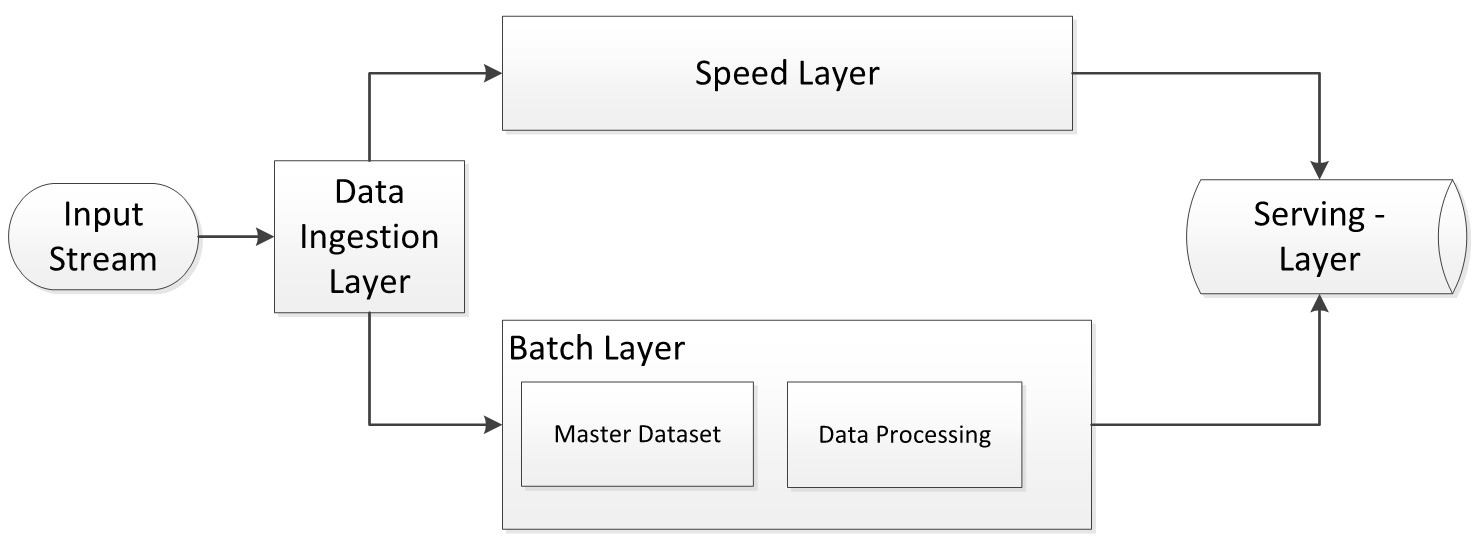
\includegraphics[width=10cm]{berle_lambda-architektur_3.jpg}
	\caption[Scheme of $\lambda$ architecture]{Scheme of $\lambda$ architecture\cite{jaxkappa}}
	\label{fig:KafkaArchitecture}
\end{figure}

\paragraph{Kappa Architectur}
This approach, designed by Confluent co-founder and CEO Jay Kreps, dispenses with batch processing and therefore only requires
\textit{Ingestion-}, \textit{Speed-} and \textit{Serving-Layer}.
This saves the development and operation of two separate layers and the time-consuming mixing of batch data with live data in the \textit{Serving-Layer}.
A prerequisite, however, is that the \textit{Ingestion-Layer} does not only pass through data volatilely,
but rather holds the raw data persistently in the \textit{Master-Dataset} as a \textit{Buffer} in order to make the raw data available again in case of a new,
not yet precalculated request or change in the \textit{Speed-Layer}.
To ensure a correct replay of the messages, the buffer is based on a canonical log, in which only messages can be added unchanged, but already saved messages can no
longer be changed or moved in their order.
This approach was named after the Greek $\kappa$ in order to illustrate both proximity and demarcation to the $\lambda$ architecture.
\cite{Kappa} \cite{Kappa2}

\begin{figure}[h]
	\centering
	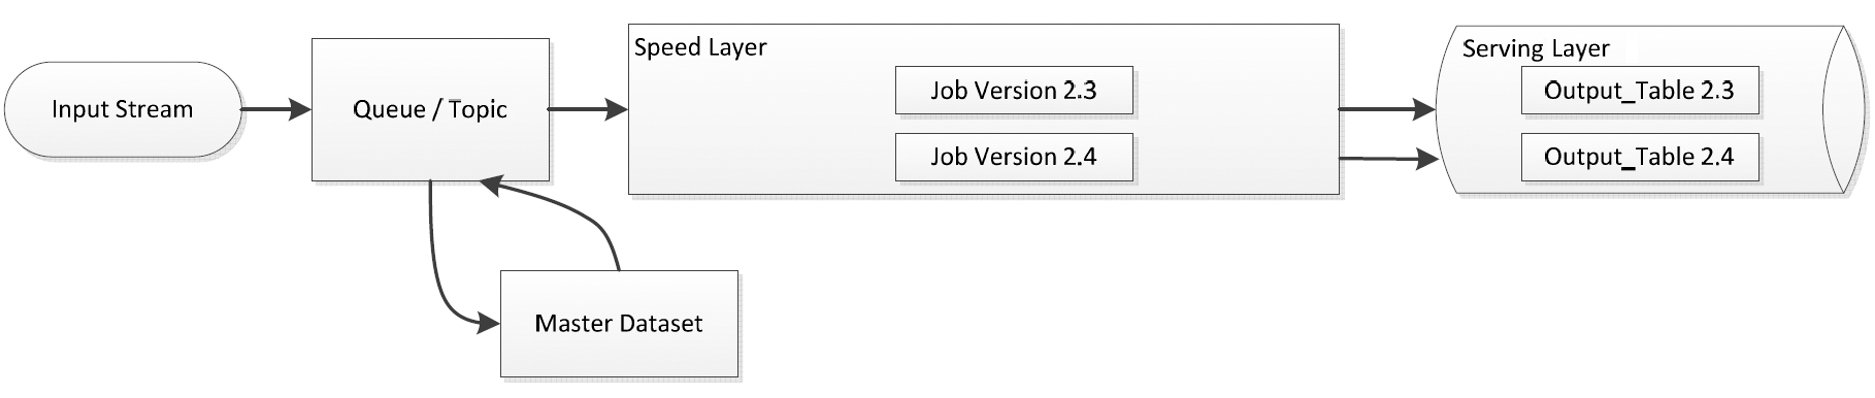
\includegraphics[width=10cm]{berle_lambda-architektur_4.jpg}
	\caption[Scheme of $\kappa$ Architectur]{Scheme of $\kappa$ Architectur\cite{jaxkappa}}
	\label{fig:KappaArchitecture}
\end{figure}

Both the Kappa and the Lamba architecture cover our requirements.
Via the input stream, any number of data sources can be accessed, in the
data ingestion layer, all collected data is stored, and then the data is processed and can be persisted in the serving layer.
The analysis part can now be executed on the serving layer.
The separation into different layers also fulfils our third requirement.

% TODO: kann das so stehen bleiben?
As explained in chapter \fullref{subsubsec:sources} our biggest data source is the Fusion \ac{API} of Yelp and
the Search \ac{API} of ImmobilienScout24.
Due to the fact that Yelp data - with the exception of the Business ID - may not be stored for more than 24 hours,\cite{YelpFaq}
the amount of data collected is manageable.

Due to the manageable amount of data that should be available to us in the end and the limited time period to complete this project,
we consciously forgo a batch layer and therefore also the Lambda architecture
in order not to unnecessarily increase the complexity of our architecture but also to reduce the processing time of data at the same time.
So we decided for a simplified version of the Kappa architecture.

In step 1 we collect the data from different data sources and write them unchanged into \gds{}
The second step consists of transporting the data into the \pg{} database from where it can be analyzed later on.
The transport included not only the simple moving of the data from the source to the target database but also the conversion of the data
into a format that has been adapted to the relational database.
Conversion, in this case, does not only mean to add additional attributes to enrich the subsequent analysis and visualization in a more meaningful way,
but also sorting out not used attributes.
The last step, the analysis of the data, was done depending on the scenario either with the Bi- and Software Analysis Software Tableau or with a Python Script and the libraries \code{pandas} and \code{matplotlib}.
\newline
The following picture shows our previously described variant of the Kappa architecture.

%TODO: picture

\subsubsection{Technical Setup}
\label{subsubsec:setup}
The Kappa architecture was realized in the programming language Python (version 3.6).
The following Python libraries were additionally installed:
\begin{itemize}
  \item \code{google-cloud-datastore}
  \item \code{sqlalchemy}
  \item \code{psycopg2}
  \item \code{requests}
  \item \code{requests\_oauthlib}
\end{itemize}
Furthermore for connecting the Yelp Fusion \ac{API} we used the python implementation of the Yelp Fusion client on GitHub\footnote{\url{https://github.com/Yelp/yelp-fusion}}
We extended this python module by our own requirements and wishes.
\newline
For the \textit{Data Cleaning} part we also wrote our own python scripts as well as some \ac{SQL} statements which we directly executed on the \pg{}.

\subsubsection{The Factory Pattern}
\label{subsubsec:factory}
As explained in \fullref{subsubsec:sources} we have different data sources from which the required data must be retrieved.
For this reason it is extremely important that our program is written in such a way that new data sources can be connected at any time.
This was realized by a combination of dynamic programming and a simple \textit{Factory Pattern}\footnote{\url{https://en.wikipedia.org/wiki/Factory_method_pattern}}.
By using the factory pattern we can abstract from the implementation logic and quickly and easily connect new data sources to the existing logic without changing anything in the underlying process.

The part of the program that is responsible for collecting and storing the data in \gds{}, is called \textbf{collector}
and that part that is responsible for transporting and mapping the raw data into \pg{} is called \textbf{transporter}
There are two modules that realize the factory pattern for both collector and transporter:

\begin{itemize}
  \item \code{factory.py}
  \item \code{creator.py}
  \item \code{collector.py}
  \item \code{transporter.py}
\end{itemize}

The module \code{factory.py} contains both the class \code{AbstractFactory}, which is an abstract variant of a concrete factory, and the class
\code{EverythingFactory} which inherits from the \code{AbstractFactory} and instantiates concrete classes of \code{collector.py} and \code{transporter.py}.
with help of the \code{creator.py} module.
This auxiliary class in this module consists of several static methods which create and return an instance of a \textit{collector}/\textit{transporter} instance.

\subsubsection{Data Ingestion}
\label{subsubsec:ingestion}
As descriped in\cite{ingestion} \textit{Data Ingestion} is the process of obtaining and importing data for immediate use or storage in a database.
In our usecase we are collecting data from various data sources, thus we need different implementation approaches on each kind of datasource.
\newline
Across all \code{collectors} data were collected from a total of five different types of data sources:
\begin{itemize}
  \item \ac{JSON}
  \item \ac{API}
  \item \ac{PDF}
  \item \ac{CSV}
  \item Web
\end{itemize}
A part that should not be underestimated is the resulting quality of the data.
While \ac{API}, \ac{CSV} and \ac{JSON} files consist of very structured data and reading them does not require much effort,
data from a \ac{PDF} file or homepage are unstructured and require a higher implementation effort and possibly an additional
\textit{Data Cleaning} step is required before using them in the analysis part to get the results that are truly reflecting the reality.
% For the implementation of \textit{Data Ingestion} the \code{collector.py} module was developed.
% Within this module is the base class for the flow logic of the concrete \textit{collectors}.
% Due to the inhomogeneity of the data sources and the associated different logic per \textit{collector}, the \code{Collector} class only contains the logic
% to store a newly created entity in the \gds{} and other auxiliary methods.
% That means that it is not possible to implement the flow logic in the base class, but be implemented to a large extent in each subclasses.
%
% To realize the \textbf{collector} and its subclasses the Python library \code{google-cloud-datastore} is used.
% The library \code{google-cloud-datastore} is a client with which it is possible to perform all known \ac{CRUD} operations for the \gds{}.

\subsubsection{Data Storage}
\label{subsubsec:storage}
In order for the data to be available for analysis and visualization, it must be read from the \gds{} and imported into the \pg{} database.
Before the data in the \pg{} can be personalized, it must be mapped to the respective table format.

This process is called \textit{Data Storage} and the Python module \code{transporter.py} was developed especially for this purpose.
In contrast to the implementation of the \code{collector} module, a large part of the \textit{Data Storage} logic is in the base class.
Only the logic for transforming the \gds{} entity to a \pg{} database table must be implemented as soon as a new
data source is to be connected.

In summary, the following steps had to be taken to develop a new \textit{transporter}:
\begin{itemize}
  \item Create a new \pg{} table with \code{sqlalchemy}
  \item  Create a new \code{<example>\_transporter.py} file that inherits from the base class.
  \item Implementation of the \code{map()} Methdode in which the \gds{} entity is received and one or more \code{sqlalchemy} object(s) are created and returned.
\end{itemize}

\subsection{Data Cleaning}
\label{subsec:cleaning}
The quality of data can be described in many dimensions like \eg{} the trustworthiness of the data source, the consistency of the data,
or their accuracy as well as their topicality. % Quelle aus PDF
Just with very unstructured data, as in our case the collected dishes from the web page speisekarte.de, the cleaning of the data is
inevitable to get a good and accurate analysis result.
However, even with supposedly good data sources such as \acp{API}, there may be errors in the data.
such as \eg{} the mixing of different languages or the lack of information.
Differences in data quality can also occur in the process of data collection.
\newline
This paragraph explains the measures taken in this project to clean up the data collected.
\paragraph{Review Count Cleaning}
In the \pg{} database the review\_count of some restaurants was assigned the value \code{NULL}.
If a new comparison with the \ylp{} \ac{API} did not result in a change of the review count,
this \code{NULL} value was replaced by the number 0.
\paragraph{Address Cleaning}
The \ac{API} of \ylp{} is designed so that an HTTP code 403 or 404 will be transmitted if no address to a restaurant
can be found.
With a python script the \ylp{} \ac{API} was addressed again to find the restaurant's address.
If still no city or postcode was found for this restaurant, this restaurant was deleted for reasons of simplicity,
since a restaurant without a postcode or city has no use for the subsequent analysis.
\paragraph{Price Range Cleaning}
In the price\_range attribute there were occasional occuring \code{NULL} values which possibly could be filled when addressing the \ylp{} \ac{API} a second time.
If this was not the case, the \code{NULL} values were filled with the mode of the price\_range from the current city.
\paragraph{City Cleaning}
Despite the fact that the \code{city} attribute of a restaurant always came from Yelp it came to a mixture of the German and English language,
so we translated the english names in its german counterparts manually.
Furthermore, the German city ''Frankfurt am Main'' was available in different spellings.
However, this could be fixed with a simple \ac{SQL} statement.
\paragraph{Buying Power Cleaning}
The data source found for acquiring the buying\_power for various german cities unfortunately contained not the buying\_power for all german cities.
We solved this isssue by replacing, the missing buying\_power with the average buying\_power in Germany in order to be able to carry out at least a rough analysis.
\paragraph{Average Purchase Price Cleaning}
Also with the average purchase price of a restaurant per m\textsuperscript{2} the original data source did not include all cities of Germany and therefore
some \code{NULL} values remained in the database.
These have been replaced with the Germany-wide average.
\paragraph{Menu Item Cleaning}
Although most of the cleaning took place after the persistence of the data in the database, the various dishes on a menu had to be
cleaned before it was written to the database.
By scraping these data directly from the web, it often happened that they were not only semantically wrong, but also containing only
special characters or an empty string.
Especially these entries without any informational content had to be removed before they were stored in the database.
This was done with several algorithms from the area of the \textit{Text Preprocessing}\footnote{Please refer to \fullref{subsec:review} to learn more about \textit{Text Preprocessing}}


\subsection{Data Cleaning}
\label{subsec:cleaning}
The quality of data can be described in many dimensions like \eg{} the trustworthiness of the data source, the consistency of the data,
or their accuracy as well as their topicality. % Quelle aus PDF
Just with very unstructured data, as in our case the collected dishes from the web page speisekarte.de, the cleaning of the data is
inevitable to get a good and accurate analysis result.
However, even with supposedly good data sources such as \acp{API}, there may be errors in the data.
such as \eg{} the mixing of different languages or the lack of information.
Differences in data quality can also occur in the process of data collection.
\newline
This paragraph explains the measures taken in this project to clean up the data collected.
\paragraph{Review Count Cleaning}
In the \pg{} database the review\_count of some restaurants was assigned the value \code{NULL}.
If a new comparison with the \ylp{} \ac{API} did not result in a change of the review count,
this \code{NULL} value was replaced by the number 0.
\paragraph{Address Cleaning}
The \ac{API} of \ylp{} is designed so that an HTTP code 403 or 404 will be transmitted if no address to a restaurant
can be found.
With a python script the \ylp{} \ac{API} was addressed again to find the restaurant's address.
If still no city or postcode was found for this restaurant, this restaurant was deleted for reasons of simplicity,
since a restaurant without a postcode or city has no use for the subsequent analysis.
\paragraph{Price Range Cleaning}
In the price\_range attribute there were occasional occuring \code{NULL} values which possibly could be filled when addressing the \ylp{} \ac{API} a second time.
If this was not the case, the \code{NULL} values were filled with the mode of the price\_range from the current city.
\paragraph{City Cleaning}
Despite the fact that the \code{city} attribute of a restaurant always came from Yelp it came to a mixture of the German and English language,
so we translated the english names in its german counterparts manually.
Furthermore, the German city ''Frankfurt am Main'' was available in different spellings.
However, this could be fixed with a simple \ac{SQL} statement.
\paragraph{Buying Power Cleaning}
The data source found for acquiring the buying\_power for various german cities unfortunately contained not the buying\_power for all german cities.
We solved this isssue by replacing, the missing buying\_power with the average buying\_power in Germany in order to be able to carry out at least a rough analysis.
\paragraph{Average Purchase Price Cleaning}
Also with the average purchase price of a restaurant per m\textsuperscript{2} the original data source did not include all cities of Germany and therefore
some \code{NULL} values remained in the database.
These have been replaced with the Germany-wide average.
\paragraph{Menu Item Cleaning}
Although most of the cleaning took place after the persistence of the data in the database, the various dishes on a menu had to be
cleaned before it was written to the database.
By scraping these data directly from the web, it often happened that they were not only semantically wrong, but also containing only
special characters or an empty string.
Especially these entries without any informational content had to be removed before they were stored in the database.
This was done with several algorithms from the area of the \textit{Text Preprocessing}\footnote{Please refer to \fullref{subsec:review} to learn more about \textit{Text Preprocessing}}


\section{Results}
\label{sec:results}

In this chapter, the results of data analysis are described through different experiments followed by an evaluation of each result and descriptive visualizations.

\subsection{Analysis}
\label{subsec:analysis}

\subsection{Monetary Analysis}
\label{subsec:moneten}
The target, mentioned in \fullref{subsec:usecase}, is to generate a turnover of 40000 euros per month. The available Budget
 is 750000 euros high. In order to generate this turnover a calculation with various parameters such as seat turnover,
 opening days, consumption and area of the guest section are required. To analyze the minimum number of seats for the
 restaurant is calculated as follows:
\begin{center}
\begin{equation}
\begin{aligned}
	min.number_{seats} = \frac{turnover.restaurant_{month}}{turnover.seat_{day} \times average.consumption_{guest} \times opening_{days}} \\
	= \frac{40000 euros}{1.5 \times 20 euros \times 26} \\
	= 51.28
\end{aligned}
\label{eq:number_seats_benchmark}
\end{equation}
\end{center}

With having the rounded minimum number of seats the calculation of the total floor space is the next step. This parameter is
 necessary for a specific query of the ImmobilienScout24 Search API \cite{ImmoScout} as well as the number of seats,
 which can be applied as range of values. The lower threshold is 52 seats and the upper threshold is 65 seats. The upper
 threshold is an increase of 25 percent. This interval can be used to calculate the required total floor area using the
 following formula:

\begin{equation}
\begin{aligned}
	total.floor.area_{min} = floorspace_{guest} \times seats_{min} \times \frac{100}{40} \\
	total.floor.area_{max} = floorspace_{guest} \times seats_{max} \times \frac{100}{40} \\
\end{aligned}
\label{eq:total_floor_space}
\end{equation}

where $floorspace_{guest}$ is the average floor space for a System-Service-Restaurant per guest \cite{FlaecheGast} and the
 percentage of the guest area is 40 percent mentioned in \cite{FlaecheGastronomie}.

 In order to apply the financing analysis, the Geo-ID of the top 10 cities is queried using the Geo \ac{API} of
 ImmobilienScout24. With this specific ID the real estate object can be queried via the Search \ac{API} and the
 defined parameters $min.number_{seats}$, $total.floor.area_{min}$, $total.floor.area_{max}$, the realestate specific
 parameter \textit{gastronomy} and gastronomytype \textit{reastaurant}.


 % link to ImmobilienScout24 Search API \cite{ImmoScout}
 % \cite{FlaecheGastronomie}, \cite{BenchmarkGastronomie}, \cite{FlaecheGast}


\subsection{Review Analysis}
\label{subsec:review}
As mentioned in \fullref{sec:introduction} it is not only the goal to propose one or more cities for the opening of a restaurant,
but also to give recommendations for qualitative characteristics of a restaurant.
\newline
For this purpose, the available reviews of a city are analyzed with the help of \ac{NLP}.
\ac{NLP} is the computer-based attempt to support any text with the help of a set of technologies and linguistic knowledge.\cite{Liddy01}
The goal of \ac{NLP} is to achieve a human-like processing of language.\cite{Liddy01}
The frequency of a certain word within the reviews - and thus also the importance of the word - can be expressed by \ac{TFIDF}.
This \ac{KPI} consists of a total of two calculations.
First the \ac{TF} is calculated.
This indicates how often a single word appears within a given document.
Mathematically this means:
\newline
\begin{equation}
  tf\textsubscript{i,j} = \frac{n\textsubscript{i,j}}{\sum_{k} n\textsubscript{i,j}}
	\label{eq:tf}
\end{equation}
Since in the pure term-frequency the totality of documents is disregarded, there is the \ac{IDF} measure.
The \ac{IDF} measure indicates how often a single word occurs within the corpus.\footnote{The totality of all documents}
It is given by the equation below.
\newline
\begin{equation}
  idf(w) = \log \frac{N}{df\textsubscript{t}}
	\label{eq:tf}
\end{equation}
Where df\textsubscript{t} is the number of documents containing the term t and N is the total number of documents in the corpus.
The factor of these two figures then forms the \ac{TFIDF} measure.\cite{droid18}
\newline
For our purposes not every single word of an yelp review is of importance.
To filter words with a low information content from an existing text, there are several methods from the area of \textit{Text Preprocessing}.
The following methods were used to improve the information density of restaurant reviews in order to calculate a meaningful \ac{TFIDF}.
\paragraph{Tokenization}
Tokenization is the process to divide a coherent sentence into single pieces, called tokens.
Beside the subdivision into single pieces, the so called stopwords and the punctuation is removed.
After Tokenization is executed on this example sentence:
\newline
\textitbf{\code{Yes, the 5 stars are deserved: here you can drink and buy the best coffee in Bochum (and maybe in the Ruhr area?).}}
\newline
only the following list of words/tokens will remain:
\newline
\textitbf{\code{['yes', '5', 'stars', 'deserved', 'drink', 'buy', 'best', 'coffee', 'bochum', 'maybe', 'ruhr', 'area']}}
\newline
The sentence structure and the grammatical correctness of the sentence are lost, but the words with a high expressiveness remain.
\paragraph{Stemming}
In linguistic morphology and information retrieval, stemming is the process for reducing inflected (or sometimes derived) words to their stem.\cite{TextMiner14}
As a result, the number of words to be analyzed is reduced and the frequency of a word is increased by reducing it to the trunk.
The following figure illustrates this fact:
\bild{stemming.png}{Stemming example}{stemming}{own representation}{0.75}
\paragraph{\acs{POS} Tagging}
\ac{POS} Tagging is another important topic in the area of \ac{NLP}.
With Tagging, words in a document are getting marked with a tag.
This tag describes the individual components of a document with their respective types \eg{} nouns, adjectives, verbs, separators, numbers, currencies and so on.
With this it is possible to filter out the types that are insignificant for the analysis, such as numbers or currencies, thus further reducing the number of words and
to increase the meaning of the remaining words.
\newline
By evaluating the most frequently used words, values can be found out on which characteristics the restaurant visitors attach the most importance.
In addition, grouping ratings into very good (5 stars) and very bad (1 star) gives the possibility to give recommendations for different restaurant characteristics which will increase the likelihood of very good ratings
and minimizes the risk of very poor ratings.
\newline
\fullref{app:review} shows words with the highest \ac{TFIDF}, which are occurring in 5-star reviews in Bochum.

\subsection{Menu Item Analysis}
\label{subsec:menu}
Neben der Frage in welcher Stadt man ein Restaurant betreiben soll oder ob man es am besten mietet oder kauft,
ist die Frage nach der Speisekarte eines der essentiellsten Themen bei der Eröffnung eines Restaurants.
\newline
Durch die gesammelten Daten der Speisekarten konnten Informationen über die angebotenen Gerichte der Restaurants in einer
Stadt in Erfahrung gebracht werden sowie die bereits vorhandenen Restaurantkategorien und die jeweils favorisierten
Gerichte eines Restaurants.
Außerdem konnten in der Datenquelle die angebotenen Services gesammelt und nach deren Häufigkeit analysiert werden.
\newline
% \newline
% \begin{minipage}[b]{0.4\textwidth}
% \begin{tabular}{llr}
\toprule
{} &                                               item &  count \\
\midrule
0   &                                          rumpsteak &      7 \\
1   &                                       gemischt eis &      4 \\
2   &                                          grilltell &      4 \\
3   &                                           tiramisu &      4 \\
4   &                                  mouss au chocolat &      4 \\
5   &                                mongo´s asia brunch &      3 \\
6   &                 mouss au chocolat birn vanillesauc &      2 \\
7   &               limonenjoghurtmouss erdbeersauc sahn &      2 \\
8   &                                              lyche &      2 \\
9   &                                  norweg lachsfilet &      2 \\
10  &                                    formaggio misto &      2 \\
11  &                                   pizza margherita &      2 \\
12  &                                     wien schnitzel &      2 \\
13  &                                           taxitell &      2 \\
14  &                                      jag schnitzel &      2 \\
15  &                                         cheeseburg &      2 \\
16  &                                              pizza &      2 \\
17  &                                            cassata &      2 \\
18  &                                     gyros uberback &      2 \\
19  &                                       crème fraîch &      2 \\
20  &                                            lammhax &      2 \\
21  &                                               menu &      2 \\
22  &                                 schnitzel wien art &      2 \\
23  &                                   gambas al ajillo &      2 \\
24  &                                           grunkohl &      2 \\
25  &                                         raubertell &      1 \\
26  &                            klein schweineschnitzel &      1 \\
27  &                               hahnchengeschnetzelt &      1 \\
28  &                                              kunef &      1 \\
29  &                                           dana sac &      1 \\
30  &                             anatoli fruhstuck tell &      1 \\
31  &                               party famili packung &      1 \\
32  &                                          namisushi &      1 \\
33  &                                         bandosushi &      1 \\
34  &                                bb doubl beef“ burg &      1 \\
35  &                              gegrillt grun spargel &      1 \\
36  &                                  tbon steak irland &      1 \\
37  &                                          sushi 4 4 &      1 \\
38  &                                     tropical desir &      1 \\
39  &                                    black sesam ice &      1 \\
40  &                                      fetakas tomat &      1 \\
41  &                                             hawaii &      1 \\
42  &                                          thunfisch &      1 \\
43  &              4 knusprig geback hahnchenbruststreif &      1 \\
44  &                                       italian burg &      1 \\
45  &                                        fajita wrap &      1 \\
46  &    lachsfilet gemusebett orangenbuttersauc krokett &      1 \\
47  &                                         royal bull &      1 \\
48  &                         red bull scaviray prosecco &      1 \\
49  &                                      veuv clicquot &      1 \\
50  &                 “caffè zentral” fruhstuck 2 person &      1 \\
51  &                                           bel paes &      1 \\
52  &                                               dolc &      1 \\
53  &                                              banan &      1 \\
54  &                                        spezialdays &      1 \\
55  &                                      postr dessert &      1 \\
56  &                              para niños kindertell &      1 \\
57  &                                          minestron &      1 \\
58  &                                       pizza funghi &      1 \\
59  &                             pizza quattro stagioni &      1 \\
60  &               hofsted schnitzel gefullt schink kas &      1 \\
61  &                                       kartoffeleck &      1 \\
62  &                                    folienkartoffel &      1 \\
63  &                                 holland kuttermatj &      1 \\
64  &                      antipasto misto della vetrina &      1 \\
65  &                                 dessert della casa &      1 \\
66  &                                       gambas salat &      1 \\
67  &                                          lust meer &      1 \\
68  &                     chick chees monst mix 2 person &      1 \\
69  &                                   hausgemacht kuch &      1 \\
70  &                    weinempfehl portugies weissherb &      1 \\
71  &                         pochiert crem tahitivanill &      1 \\
72  &                          braciol di bufalo al ragu &      1 \\
73  &                               spezzatino di bufalo &      1 \\
74  &                            fettin pizzaiola capres &      1 \\
75  &                            susskartoffel dipp wahl &      1 \\
76  &                          ofenkartoffel heringsstip &      1 \\
77  &  biet taglich 2 supp eintopf vegetar vegan supp... &      1 \\
78  &                                   salat „italiano“ &      1 \\
79  &                                     salat „espana“ &      1 \\
80  &                                     salat „cesare“ &      1 \\
81  &                                     sambus 3 stuck &      1 \\
82  &          masa beirut vorspeis hauptgericht dessert &      1 \\
83  &                          masa maroush hauptgericht &      1 \\
84  &                                     panang curry p &      1 \\
85  &                                 flamed tandoori ft &      1 \\
86  &                                     mongo´s bbq mb &      1 \\
87  &                                   salat „lendchen“ &      1 \\
88  &                                    klein chefsalat &      1 \\
89  &                     schollenfilet „finkenward art“ &      1 \\
90  &                                  insalata di pollo &      1 \\
91  &                                    antipasto misto &      1 \\
92  &                               combinazion di mamma &      1 \\
93  &                                          mild matj &      1 \\
94  &                                      andechs pfann &      1 \\
95  &                         geschnetzelt schweinefilet &      1 \\
96  &                                  pizza capricciosa &      1 \\
97  &                                    pizza carpaccio &      1 \\
98  &                                 spaghetti bolognes &      1 \\
99  &      cola fanta sprit cola light 1l flasch mitnehm &      1 \\
100 &                         lambrusco rosso bianco 07l &      1 \\
101 &                                           bier 05l &      1 \\
102 &                       knusprig ent verschied gemus &      1 \\
103 &                       knusprig ent rot curry gemus &      1 \\
104 &                    knusprig ent susssau sauc gemus &      1 \\
105 &                                         tbon steak &      1 \\
106 &                                     el gauchoplatt &      1 \\
107 &                                   pfefferhuftsteak &      1 \\
108 &                           gross gemischt salattell &      1 \\
109 &                                  schweineschnitzel &      1 \\
110 &                                         vanilleeis &      1 \\
111 &                          pizza rucola e pomodorini &      1 \\
112 &                                          gamberoni &      1 \\
113 &                                            churros &      1 \\
114 &                                 quesadillas capres &      1 \\
115 &                                       club burrito &      1 \\
116 &                                champignonschnitzel &      1 \\
117 &                                          lammsteak &      1 \\
118 &                                            bento 1 &      1 \\
119 &                                   karaag nudelsupp &      1 \\
120 &                                     gem sushi tell &      1 \\
121 &                                        malai kofta &      1 \\
122 &                                       jaffna curry &      1 \\
123 &       butterzart huhnerbrust plus keul nuss batura &      1 \\
124 &                                         thainudeln &      1 \\
125 &                             klein frisch salattell &      1 \\
126 &                                 frisch gartensalat &      1 \\
127 &                                             browni &      1 \\
128 &                                       stoned prawn &      1 \\
129 &                              the real beef rib eye &      1 \\
130 &                          schnitzeltasch querenburg &      1 \\
131 &                             schnitzeltasch hofsted &      1 \\
132 &                                         innenstadt &      1 \\
133 &                                  chipiron rellenos &      1 \\
134 &                                 boqueron al vinagr &      1 \\
135 &                                  ciruelas en bacón &      1 \\
136 &                                     wasabi special &      1 \\
137 &                                     japan reiskuch &      1 \\
138 &                                       schwarz tell &      1 \\
139 &                                          fresh fit &      1 \\
140 &                                       salat saison &      1 \\
141 &                                 hahnchenburstfilet &      1 \\
142 &                                saganaki me sousámi &      1 \\
143 &                                            taramas &      1 \\
144 &                                           riganato &      1 \\
145 &                                         chili sauc &      1 \\
146 &                                       erdnuss sauc &      1 \\
147 &                                     sussesauersauc &      1 \\
148 &                                         jagerpfann &      1 \\
149 &                                    ratsherrenpfann &      1 \\
150 &                                        kasslernack &      1 \\
151 &                                        gemuseplatt &      1 \\
152 &                           gebrat ent a la szechuan &      1 \\
153 &                        rindfleisch gebrat zwiebeln &      1 \\
154 &                               gansekeul vorbestell &      1 \\
155 &                                        gamba pfann &      1 \\
156 &                                         mediterran &      1 \\
157 &                                         currywurst &      1 \\
158 &                                         putensteak &      1 \\
159 &                                     8 hahnchenteil &      1 \\
160 &                                          zing burg &      1 \\
161 &                                         filet burg &      1 \\
162 &                                          fischtell &      1 \\
163 &                                     garnel paniert &      1 \\
164 &                                    calamaris pfann &      1 \\
165 &                                         filetsteak &      1 \\
166 &                                      epigrammplatt &      1 \\
167 &                            seniorentell wahl salat &      1 \\
168 &       gemischt eis heiss amarenakirsch vanillesahn &      1 \\
169 &                       geback apfelring vanillesoss &      1 \\
170 &                           klein schnitzel apfelmus &      1 \\
171 &                           72 feuerspiess flambiert &      1 \\
172 &                                   404 trikala tell &      1 \\
173 &                                     132 filetsteak &      1 \\
174 &                                         acadi burg &      1 \\
175 &                                           tzatziki &      1 \\
176 &                                              aioli &      1 \\
177 &                                         putenfilet &      1 \\
178 &                                         herm platt &      1 \\
179 &                                          jalapeños &      1 \\
180 &                                   the awesom duffl &      1 \\
181 &                             brooklyn byt cheesecak &      1 \\
182 &                                  87 rotbarschfilet &      1 \\
183 &                              82 chines hummerkrabb &      1 \\
184 &                              k8 peking ent pro per &      1 \\
185 &                                              gyros &      1 \\
186 &                                      nikolausplatt &      1 \\
187 &                             lammcarré krauterkrust &      1 \\
188 &                             milchkalbsleb pet farm &      1 \\
189 &                               schnitzel hollandais &      1 \\
190 &                                 holstein schnitzel &      1 \\
191 &                                 rumpsteak art haus &      1 \\
192 &                                      pfefferspiess &      1 \\
193 &                                       vegetar tell &      1 \\
194 &      gebrat poulardenbrust tranch ratatouillegemus &      1 \\
195 &                             schnitzel holstein art &      1 \\
196 &                    kalbsleb berlin art butt gebrat &      1 \\
197 &                  filet bif de lomo zart stuck rind &      1 \\
198 &                                        zanderfilet &      1 \\
199 &                                    zwiebelrostbrat &      1 \\
200 &                                        classic set &      1 \\
201 &                                          futo maki &      1 \\
202 &                                          raup roll &      1 \\
203 &                rucola parmesan gerostet pinienkern &      1 \\
204 &                           warm vorspeisenvariation &      1 \\
205 &                   mouss au chocolat gluhweinkirsch &      1 \\
206 &                spaghetti shrimps gemus tomatensauc &      1 \\
207 &                           spaghetti schafskas oliv &      1 \\
208 &                    spaghetti pesto kl tomatensalat &      1 \\
209 &             eis schokoladensauc amarettosirup beer &      1 \\
210 &                                           tag tort &      1 \\
211 &                                               lach &      1 \\
212 &                                        bayer crème &      1 \\
213 &                           panna cotta pinha colada &      1 \\
214 &                       lemonchocolat cheesecak glas &      1 \\
215 &                                               saft &      1 \\
216 &                                              milch &      1 \\
217 &                                             zitron &      1 \\
218 &                                 roastbeefschnittch &      1 \\
219 &                             schnitzel onkel martin &      1 \\
220 &                                     jagerschnitzel &      1 \\
221 &                                    insalata rimini &      1 \\
222 &                                 insalata capriccio &      1 \\
223 &                                     parma e rucola &      1 \\
224 &                                        weiss mouss &      1 \\
225 &                                     cheesecak tart &      1 \\
226 &                                          bunt beet &      1 \\
227 &                                schweineruckensteak &      1 \\
228 &                          knusprig gebrat bauernent &      1 \\
229 &                             schweinefiletmedaillon &      1 \\
230 &                                        mauricetell &      1 \\
231 &                  auswahl international rohmilchkas &      1 \\
232 &                                           manchego &      1 \\
233 &                      hausgemacht eissort pro kugel &      1 \\
234 &                                     candy bar shak &      1 \\
235 &                             burg burg bun serviert &      1 \\
236 &                                              micro &      1 \\
237 &                                       apfelstrudel &      1 \\
238 &                                      steaksandwich &      1 \\
239 &                                               burg &      1 \\
240 &                                    wienerschnitzel &      1 \\
241 &                                          sauerbrat &      1 \\
242 &                    franz ferdinand kaiserschnitzel &      1 \\
243 &                                            mousaka &      1 \\
244 &                                            bifteki &      1 \\
245 &                                 portion spanferkel &      1 \\
246 &                           ice cream paletas berlin &      1 \\
247 &                                  kokos panna cotta &      1 \\
248 &                                vietnames coffe pie &      1 \\
249 &                            filetspitz waldpilzrahm &      1 \\
250 &                                          lammkarre &      1 \\
251 &                                       rinderroulad &      1 \\
252 &                                          riesenrad &      1 \\
253 &                           rumpsteak bratkartoffeln &      1 \\
254 &                                            gut ute &      1 \\
255 &                              lammfilet al pep verd &      1 \\
256 &                              rinderfilet grill xxl &      1 \\
257 &                                rumpsteak grill xxl &      1 \\
258 &                                       1 margherita &      1 \\
259 &                                   pizzablech mista &      1 \\
260 &                           102 insalata capricciosa &      1 \\
261 &                                        panna cotta &      1 \\
262 &                          tortellini alla romanella &      1 \\
263 &                               gamberoni fradiavolo &      1 \\
264 &                             gamberoni alla griglia &      1 \\
265 &                        echt donninghaus currywurst &      1 \\
266 &                                  frikadell spezial &      1 \\
267 &                                ritterburghaussalat &      1 \\
268 &                                      geback ananas &      1 \\
269 &                                       geback banan &      1 \\
270 &                                     kugel eis wahl &      1 \\
271 &                                 hausgemacht lasagn &      1 \\
272 &                                 insalata contadina &      1 \\
273 &                               rucolasalat parmesan &      1 \\
274 &                        schnitzelvariation chef art &      1 \\
275 &                                   kolpinghauspfann &      1 \\
276 &                                  paris zwiebelsupp &      1 \\
277 &                                           95 manti &      1 \\
278 &                                  71 yogurtlu adana &      1 \\
279 &                                      38 et corbasi &      1 \\
280 &                                              astic &      1 \\
281 &                                     insalata mista &      1 \\
282 &                                    antipasti misti &      1 \\
283 &                                       lasagneblech &      1 \\
284 &                              pizzablech margherita &      1 \\
285 &                                          angebot 4 &      1 \\
286 &            klein schnitzel wien art rostkartoffeln &      1 \\
287 &                                       schnorritell &      1 \\
288 &                                lammruck zwiebelmus &      1 \\
289 &                             rindfleisch szchuanart &      1 \\
290 &                                           reiswein &      1 \\
291 &                                       pflanmenwein &      1 \\
292 &                                           dondurma &      1 \\
293 &                                      meyv salatasi &      1 \\
294 &                                    arkadas tatlisi &      1 \\
295 &                      ganz holt gan beilag 4 person &      1 \\
296 &  neuling steak schmorzwiebeln rostkartoffeln salat &      1 \\
297 &                     krauterknoblauchsuppch crouton &      1 \\
298 &                                         jhardareis &      1 \\
299 &                                        mango mouss &      1 \\
300 &                                        mango kulfi &      1 \\
301 &                                            special &      1 \\
302 &                                           bolognes &      1 \\
303 &                                        pizza mista &      1 \\
304 &                                        pizza salam &      1 \\
305 &                               hausgemacht tiramisu &      1 \\
306 &                                tortellini al forno &      1 \\
307 &                                 tagliatell nostran &      1 \\
308 &                                insalata com bochum &      1 \\
309 &                                  gnocchi al capres &      1 \\
310 &                              gnocchi ai 4 formaggi &      1 \\
311 &                                       mykonos tell &      1 \\
312 &                                     akropolis tell &      1 \\
313 &                                        babykalamar &      1 \\
314 &                                    gyros “artemis” &      1 \\
315 &                                          gyrostell &      1 \\
316 &                       tortelloni al pistaccio verd &      1 \\
317 &                             parmigiana di melanzan &      1 \\
318 &                                               penn &      1 \\
319 &                                   gemischt eisbech &      1 \\
320 &                                frisch nordseekrabb &      1 \\
321 &                               pfefferrahmschnitzel &      1 \\
322 &                                     marathon platt &      1 \\
323 &                                   fruhstucksbuffet &      1 \\
324 &             hawaiitoast schink ananas kas uberback &      1 \\
325 &        thunfischtoast schink zwiebeln kas uberback &      1 \\
326 &                                           kasetell &      1 \\
327 &                               hausgemacht tiramisù &      1 \\
328 &     3gangeuberraschungsmenu wahlweis fisch fleisch &      1 \\
329 &  kartoffellauchroulad brickteigmantel krautersa... &      1 \\
330 &                                      raffaellobech &      1 \\
331 &                                 meeresfruchtepasta &      1 \\
332 &                                          leberkas´ &      1 \\
333 &                                    biet vorbestell &      1 \\
334 &                        mettwurstpfann „haus spitz“ &      1 \\
335 &                                          pfannkuch &      1 \\
336 &                         gegrillt maishahnchenbrust &      1 \\
337 &                         gegrillt schweinemedaillon &      1 \\
338 &                                gegrillt lachsfilet &      1 \\
339 &                                    hawaiischnitzel &      1 \\
340 &                    klein rumpsteak pomm frit salat &      1 \\
341 &                 schnitzel wien art pomm frit gemus &      1 \\
342 &  original wien kalbsschnitzel bratkartoffeln kn... &      1 \\
343 &  sauerbrat ochsenbrust apfelrotkraut kartoffelnock &      1 \\
344 &  gebrat salbeilammfilet gemus provenc rucolakar... &      1 \\
345 &                                  mooh phad noa mai &      1 \\
346 &                                     mooh phad kink &      1 \\
347 &                              mooh phad bai gra pao &      1 \\
348 &       frisch datteln buttersaucerresauc vanilleeis &      1 \\
349 &                          charolaisfilet barolosauc &      1 \\
350 &                                gemusetell waldhaus &      1 \\
351 &                                               leck &      1 \\
352 &                                  chorizo a la miel &      1 \\
353 &                                aceitunas mezcladas &      1 \\
354 &                                   champinon ajillo &      1 \\
355 &                         137 spaghetti aglio e olio &      1 \\
356 &                           52 pennetomatensahnesauc &      1 \\
357 &                                       86 sauerrahm &      1 \\
358 &                           vanillequark himbeersauc &      1 \\
359 &                                           orektika &      1 \\
360 &                                    statt pomm reis &      1 \\
361 &                                    penelopepfannch &      1 \\
362 &                                 sousukakia spezial &      1 \\
363 &                                      juni – august &      1 \\
364 &                                          april mai &      1 \\
365 &                                            septemb &      1 \\
366 &                                  dessert trattoria &      1 \\
367 &                                            casatta &      1 \\
368 &                                        fischstabch &      1 \\
369 &                                 hahnchenbrustfilet &      1 \\
370 &                                    klein schnitzel &      1 \\
371 &                                       gourmet tell &      1 \\
372 &                                           polapola &      1 \\
373 &                    reisauflauf aromatisiert pflaum &      1 \\
374 &  filet wel kartoffelkrust sahnig schwarzwurzelg... &      1 \\
375 &                                   pizza prosciutto &      1 \\
376 &                                            tartufo &      1 \\
377 &                                 schwarz tagliatell &      1 \\
378 &                                         tagliatell &      1 \\
379 &                                       caesar salad &      1 \\
380 &  lachsforellenfiletmit stielmusrhabarbergemus e... &      1 \\
381 &        spaghettini tomat knoblauch rucola parmesan &      1 \\
382 &                            spaghetti alla bolognes &      1 \\
383 &                                 carpaccio di manzo &      1 \\
384 &                              mozzarella di buffola &      1 \\
385 &                                        gesund tell &      1 \\
386 &                                             obazda &      1 \\
387 &                                    espressopudding &      1 \\
388 &                              gewurzt couscoussalat &      1 \\
389 &                                          welsfilet &      1 \\
390 &                          tapas variadas de pescado &      1 \\
391 &                                champiñon al ajillo &      1 \\
392 &                                          eis heiss &      1 \\
393 &                                    melitzanosalata &      1 \\
394 &                                holzfallerschnitzel &      1 \\
395 &                                       versch belag &      1 \\
396 &                                             funghi &      1 \\
397 &                                   tomat mozzarella &      1 \\
398 &                                 gegrillt gansebrat &      1 \\
399 &                schweinefiletmedaillon iber schwein &      1 \\
400 &                             gamberoni alia griglia &      1 \\
401 &                                        combinazion &      1 \\
402 &                                      pizza tiziana &      1 \\
403 &                               schwein iber schwein &      1 \\
404 &                            medaillon schweinefilet &      1 \\
405 &                                     gemischt salat &      1 \\
406 &                                    gross salattell &      1 \\
407 &                                         kegl toast &      1 \\
408 &                                           eiskaffe &      1 \\
409 &                                       pfannengyros &      1 \\
410 &                            insalata di tonno gross &      1 \\
411 &                            pizza buongustaia klein &      1 \\
412 &                               pizza broccoli klein &      1 \\
413 &                                  schultenhof pfann &      1 \\
414 &                                    seezungenrollch &      1 \\
415 &                            doppelt portion fleisch &      1 \\
416 &                                   chili chees burg &      1 \\
417 &                                         veggi burg &      1 \\
418 &                      gold stabchenspezial 2 person &      1 \\
419 &                            sichuanspezial 2 person &      1 \\
420 &                           shanghaispezial 2 person &      1 \\
421 &                                          schnitzel &      1 \\
422 &                                         damentoast &      1 \\
423 &                                 doppelt currywurst &      1 \\
424 &          geback ent mandeln bambusspross chamignon &      1 \\
425 &  babipangang fein geschnitt – geback schweinefl... &      1 \\
426 &                                   ya kai ngau chap &      1 \\
427 &                      maccheroni gyros kas uberback &      1 \\
428 &                  maccaroni tortellini kas uberback &      1 \\
429 &                       maccheroni verd kas uberback &      1 \\
430 &                             rigatoni alla giovanni &      1 \\
431 &                                     piccata romana &      1 \\
432 &                              fettina alla bolognes &      1 \\
433 &                                           sis tell &      1 \\
434 &                                         donertasch &      1 \\
435 &                                        hirtensalat &      1 \\
436 &                                          steaktell &      1 \\
437 &                            gyros uberback komplett &      1 \\
438 &                                       barbarenburg &      1 \\
439 &                                          elfenburg &      1 \\
440 &                                   elsass flammkuch &      1 \\
441 &                                             yanmei &      1 \\
442 &                                       bananensplit &      1 \\
443 &                            shrimps verschied gemus &      1 \\
444 &  ausflug trop huhnerbrust bambus morcheln china... &      1 \\
445 &          neugier huhn huhnerbrust chin pilz bambus &      1 \\
446 &                                       spaghettieis &      1 \\
447 &                                           kiddybox &      1 \\
448 &                                         tagliolini &      1 \\
449 &                                            gnocchi &      1 \\
450 &                                    gebrat kalbsleb &      1 \\
451 &                                   zwiebelschnitzel &      1 \\
452 &                                       teufelssteak &      1 \\
453 &                                      12 jagerpfann &      1 \\
454 &                                             specki &      1 \\
455 &                                           ruhrpott &      1 \\
456 &                                  tagliatell salmon &      1 \\
457 &                                         schaschlik &      1 \\
458 &                                         molos tell &      1 \\
459 &                       saltimbocca wolfsbarschfilet &      1 \\
460 &                              dessert tris la scala &      1 \\
461 &           dorad ganz krauterbutt salat beilag wahl &      1 \\
462 &                 burgunderbrat rotkohl kartoffeltal &      1 \\
463 &  cordon bleu schweinefilet rahmwirsing bratkart... &      1 \\
464 &                                  schweinemedaillon &      1 \\
465 &                                 westfal herrencrem &      1 \\
466 &                                   seezung gegrillt &      1 \\
467 &                               gemischt desserttell &      1 \\
468 &                                  sutlac mittelsuss &      1 \\
469 &                            spanisch caramelpudding &      1 \\
470 &                               blaubartz kaptensdin &      1 \\
471 &                                    pollitocalimero &      1 \\
472 &                                            stifado &      1 \\
473 &                          arnaki frikass me marouli &      1 \\
474 &                         giouvetsi arni me chilopit &      1 \\
475 &                gambas speckmantel rosa pfeffersauc &      1 \\
476 &                      gebrat doradenfilet krauterol &      1 \\
477 &        filet weiss wel tomat mozzarella gratiniert &      1 \\
478 &                                   zigeun schnitzel &      1 \\
479 &                                        beyti kebap &      1 \\
480 &                                       imam bayildi &      1 \\
481 &                                       karis izgara &      1 \\
482 &                           plato de pescado variado &      1 \\
483 &                             backpflaum speckmantel &      1 \\
484 &                                     massala gambas &      1 \\
485 &                            massala mixed huhn rind &      1 \\
486 &                        massala vegetar saisongemus &      1 \\
487 &                                           tres doc &      1 \\
488 &                                      tod schokolad &      1 \\
489 &                                         pudim flan &      1 \\
490 &                                          pomm frit &      1 \\
491 &                                  gebrat reisnudeln &      1 \\
492 &                                      gebrat nudeln &      1 \\
493 &                                   gross eisportion &      1 \\
494 &                                 92 krabbencocktail &      1 \\
495 &                                       crème brûlée &      1 \\
496 &                              gemischt eis 3 kugeln &      1 \\
497 &                               warm apfelbirnentart &      1 \\
498 &                       hausgemacht blueberry muffin &      1 \\
499 &                                    orang dreierlei &      1 \\
500 &                   pizza hawaii spezial tomatensauc &      1 \\
501 &                            pizza texas tomatensauc &      1 \\
502 &                                      pizza gourmet &      1 \\
503 &                              paelha a moda de casa &      1 \\
504 &                                prato misto de peix &      1 \\
505 &                                      gambas picant &      1 \\
\bottomrule
\end{tabular}

% \end{minipage}
% \begin{minipage}[b]{0.2\textwidth}
% \begin{tabular}{llr}
\toprule
{} &                                               item &  count \\
\midrule
0    &                                              pizza &    696 \\
1    &                                          schnitzel &    302 \\
2    &                                              gyros &    148 \\
3    &                                              curry &     87 \\
4    &                                               lach &     67 \\
5    &                                      gebrat nudeln &     62 \\
6    &                                        gebrat reis &     55 \\
7    &                                            baguett &     54 \\
8    &                                        rinderfilet &     54 \\
9    &                                             garnel &     49 \\
10   &                                    schweinefleisch &     49 \\
11   &                                          carpaccio &     47 \\
12   &                                             hawaii &     44 \\
13   &                                              steak &     42 \\
14   &                                          rumpsteak &     39 \\
15   &                                              krabb &     38 \\
16   &                                          thunfisch &     37 \\
17   &                                        rindfleisch &     37 \\
18   &                                              aioli &     36 \\
19   &                                      huhnerfleisch &     35 \\
20   &                                       pizza funghi &     34 \\
21   &                                     bratkartoffeln &     34 \\
22   &                                         filetsteak &     33 \\
23   &                                               huhn &     32 \\
24   &                                         putensteak &     32 \\
25   &                                               tell &     31 \\
26   &                                   pizza margherita &     31 \\
27   &                                         currywurst &     31 \\
28   &                                         prosciutto &     31 \\
29   &                                       pizza salami &     29 \\
30   &                                     jagerschnitzel &     29 \\
31   &                                             calzon &     29 \\
32   &                                          kartoffel &     28 \\
33   &                                        pizza tonno &     28 \\
34   &                                          ziegenkas &     28 \\
35   &                                 hahnchenbrustfilet &     27 \\
36   &                                          pomm frit &     26 \\
37   &                                        gulaschsupp &     25 \\
38   &                                             salami &     25 \\
39   &                                     gemischt salat &     25 \\
40   &                                             nachos &     25 \\
41   &                                            spezial &     25 \\
42   &                                             gebrat &     24 \\
43   &                                      fruhlingsroll &     24 \\
44   &                                         bruschetta &     24 \\
45   &                                             capres &     24 \\
46   &                                       lammkotelett &     24 \\
47   &                                 spaghetti bolognes &     24 \\
48   &                                           wien art &     24 \\
49   &                                           bolognes &     24 \\
50   &                                            krokett &     23 \\
51   &                                       gemischt eis &     23 \\
52   &                                             galett &     23 \\
53   &                                            bifteki &     23 \\
54   &                                        bauernsalat &     23 \\
55   &                                              kebap &     22 \\
56   &                                           uberback &     22 \\
57   &                                              speck &     22 \\
58   &                                       chick nugget &     21 \\
59   &                                           saganaki &     21 \\
60   &                                         huhnersupp &     20 \\
61   &                                               feta &     20 \\
62   &                                              banan &     20 \\
63   &                                              klein &     20 \\
64   &                                      frutti di mar &     20 \\
65   &                                              gemus &     20 \\
66   &                                              unagi &     19 \\
67   &                                        tomatensupp &     19 \\
68   &                                          vegetaria &     19 \\
69   &                                             geback &     19 \\
70   &                                spaghetti carbonara &     19 \\
71   &                                           broccoli &     19 \\
72   &                                            sashimi &     18 \\
73   &                                        panna cotta &     18 \\
74   &                                     insalata mista &     18 \\
75   &                                        hausgemacht &     18 \\
76   &                                              salat &     18 \\
77   &                                         entenbrust &     18 \\
78   &                                               lamm &     18 \\
79   &                                            diavolo &     18 \\
80   &                                              sushi &     17 \\
81   &                                              bacon &     17 \\
82   &                                               tofu &     17 \\
83   &                                              mango &     17 \\
84   &                                             napoli &     17 \\
85   &                                            scampis &     17 \\
86   &                                          grilltell &     17 \\
87   &                                   quattro stagioni &     16 \\
88   &                                            spinaci &     16 \\
89   &                                        cordon bleu &     16 \\
90   &                                          cevapcici &     16 \\
91   &                                          flammkuch &     16 \\
92   &                                             nigiri &     15 \\
93   &                                                kas &     15 \\
94   &                                  mouss au chocolat &     15 \\
95   &                                    vitello tonnato &     15 \\
96   &                                              pasta &     15 \\
97   &                                        hummerkrabb &     15 \\
98   &                                              tapas &     15 \\
99   &                                            risotto &     15 \\
100  &                                           calamari &     15 \\
101  &                                         mozzarella &     15 \\
102  &                                        lammfleisch &     15 \\
103  &                                         gamberetti &     15 \\
104  &                                           gegrillt &     14 \\
105  &                                         champignon &     14 \\
106  &                                          spaghetti &     14 \\
107  &                                               wien &     14 \\
108  &                                franzos zwiebelsupp &     14 \\
109  &                                             schink &     14 \\
110  &                                           knusprig &     14 \\
111  &                                              gross &     14 \\
112  &                                  schweinemedaillon &     14 \\
113  &                                       crème fraîch &     14 \\
114  &                                             temaki &     13 \\
115  &                                                sak &     13 \\
116  &                                             spinat &     13 \\
117  &                                          bratwurst &     13 \\
118  &                                          frikadell &     13 \\
119  &                                   spaghetti napoli &     13 \\
120  &                                   zwiebelschnitzel &     13 \\
121  &                                              tonno &     13 \\
122  &                                           tiramisu &     13 \\
123  &                                  zigeunerschnitzel &     13 \\
124  &                                      schweinesteak &     13 \\
125  &                                               koft &     12 \\
126  &                                               pita &     12 \\
127  &                                            joghurt &     12 \\
128  &                                         gemusesupp &     12 \\
129  &                                          antipasti &     12 \\
130  &                                   quattro formaggi &     12 \\
131  &                                tortellini al forno &     12 \\
132  &                                             funghi &     12 \\
133  &                                        pizzabrotch &     12 \\
134  &                                         gorgonzola &     12 \\
135  &                                               rind &     12 \\
136  &                                             waffel &     12 \\
137  &                                             frisch &     11 \\
138  &                                        hausgebeizt &     11 \\
139  &                                             maguro &     11 \\
140  &                                           teriyaki &     11 \\
141  &                                          pfannkuch &     11 \\
142  &                                    lasagn al forno &     11 \\
143  &                                          nudelsupp &     11 \\
144  &                                             lasagn &     11 \\
145  &                                         margherita &     11 \\
146  &                                             forell &     11 \\
147  &                                            falafel &     11 \\
148  &                                          huftsteak &     11 \\
149  &                                            biryani &     11 \\
150  &                                            chorizo &     11 \\
151  &                                              chick &     11 \\
152  &                                          blutwurst &     10 \\
153  &                                         glasnudeln &     10 \\
154  &                                             salmon &     10 \\
155  &                                          roastbeef &     10 \\
156  &                               klein gemischt salat &     10 \\
157  &                                           zwiebeln &     10 \\
158  &                                              parma &     10 \\
159  &                                                sat &     10 \\
160  &                                            toscana &     10 \\
161  &                                              pollo &     10 \\
162  &                                             masala &     10 \\
163  &                                         dolmadakia &     10 \\
164  &                                             zaziki &     10 \\
165  &                                         metaxasauc &     10 \\
166  &                                              mista &     10 \\
167  &                                   pfefferschnitzel &     10 \\
168  &                       gemischt salat frisch spross &     10 \\
169  &                                             fajita &      9 \\
170  &                                         cheeseburg &      9 \\
171  &                                    kartoffelgratin &      9 \\
172  &                                               sauc &      9 \\
173  &                                        nasi goreng &      9 \\
174  &                                          minestron &      9 \\
175  &                               insalata capricciosa &      9 \\
176  &                             schweinefiletmedaillon &      9 \\
177  &                                               brot &      9 \\
178  &                                               matj &      9 \\
179  &                                             italia &      9 \\
180  &                                        gurkensalat &      9 \\
181  &                                           tortilla &      9 \\
182  &                                            tintenf &      9 \\
183  &                                            paniert &      9 \\
184  &                                          lammfilet &      9 \\
185  &                                           vindaloo &      9 \\
186  &                            spaghetti frutti di mar &      9 \\
187  &                                      schweinefilet &      9 \\
188  &                                   geback camembert &      9 \\
189  &                                             scharf &      9 \\
190  &                                             nudeln &      9 \\
191  &                                               reis &      9 \\
192  &                                      geback ananas &      9 \\
193  &                                       ent knusprig &      9 \\
194  &                                           leberkas &      8 \\
195  &                                            vegetar &      8 \\
196  &                                           kizartma &      8 \\
197  &                                                ebi &      8 \\
198  &                                                rot &      8 \\
199  &                                         stramm max &      8 \\
200  &                                         griechisch &      8 \\
201  &                                           remoulad &      8 \\
202  &                                              grill &      8 \\
203  &                                     kalbsschnitzel &      8 \\
204  &                                            wurfeln &      8 \\
205  &                                  pizza capricciosa &      8 \\
206  &                                        zwiebelsupp &      8 \\
207  &                                  putengeschnetzelt &      8 \\
208  &                                          fischsupp &      8 \\
209  &                                     kartoffelsalat &      8 \\
210  &                                        saltimbocca &      8 \\
211  &                                          schafskas &      8 \\
212  &                                                  6 &      8 \\
213  &                                    weinbergschneck &      8 \\
214  &                                           tandoori &      8 \\
215  &                                        capricciosa &      8 \\
216  &                                         hollandais &      8 \\
217  &                                          carbonara &      8 \\
218  &                                           maiskolb &      8 \\
219  &                                       caesar salad &      8 \\
220  &                                      zigeunerwurst &      8 \\
221  &                                       meeresfrucht &      8 \\
222  &                                       knusprig ent &      8 \\
223  &                                            cipolla &      8 \\
224  &                                          sauerbrat &      8 \\
225  &                                            krustch &      8 \\
226  &                                         vanilleeis &      7 \\
227  &                                                ika &      7 \\
228  &                                            tom yam &      7 \\
229  &                                             kimchi &      7 \\
230  &                                       toast hawaii &      7 \\
231  &                                  warm apfelstrudel &      7 \\
232  &                                                  “ &      7 \\
233  &                                      knoblauchbrot &      7 \\
234  &                                   tomat mozzarella &      7 \\
235  &                                               supp &      7 \\
236  &                                                ent &      7 \\
237  &                                    folienkartoffel &      7 \\
238  &                                        zanderfilet &      7 \\
239  &                                            paesana &      7 \\
240  &                                            paprika &      7 \\
241  &                                              dorad &      7 \\
242  &                                            omelett &      7 \\
243  &                                              melon &      7 \\
244  &                                 spaghetti al forno &      7 \\
245  &                                           gemischt &      7 \\
246  &                                           original &      7 \\
247  &                                       buffalo wing &      7 \\
248  &                                   pfefferrumpsteak &      7 \\
249  &                                            ketchup &      7 \\
250  &                                            schwein &      7 \\
251  &                                         krautsalat &      7 \\
252  &                                        pljeskavica &      7 \\
253  &                                         jagerwurst &      7 \\
254  &                                             scampi &      7 \\
255  &                                             metaxa &      7 \\
256  &                                            portion &      7 \\
257  &                                   tomatencremesupp &      7 \\
258  &                                       kas uberback &      7 \\
259  &                                                 ei &      7 \\
260  &                                      pizza cipolla &      7 \\
261  &                              knusprig gerostet ent &      7 \\
262  &                                       avocado maki &      6 \\
263  &                                    california maki &      6 \\
264  &                                       baked potato &      6 \\
265  &                                           insalata &      6 \\
266  &                                         ratatouill &      6 \\
267  &                                             ananas &      6 \\
268  &                                    insalata italia &      6 \\
269  &                                         cannelloni &      6 \\
270  &                                          spiegelei &      6 \\
271  &                                 champignonrahmsauc &      6 \\
272  &                                               kalb &      6 \\
273  &                                         chick wing &      6 \\
274  &                                   wildkrautersalat &      6 \\
275  &                                  blattsalat saison &      6 \\
276  &                                              tomat &      6 \\
277  &                                     rotbarschfilet &      6 \\
278  &                                       mongo´s asia &      6 \\
279  &                                              satay &      6 \\
280  &                                         lachsfilet &      6 \\
281  &                                             fritti &      6 \\
282  &                                    spaghetti tonno &      6 \\
283  &                                       tomatensalat &      6 \\
284  &                                     thunfischsalat &      6 \\
285  &                                              filet &      6 \\
286  &                                        krauterbutt &      6 \\
287  &                                          fischtell &      6 \\
288  &                                             mutton &      6 \\
289  &                                               menu &      6 \\
290  &                                          mayonnais &      6 \\
291  &                                             browni &      6 \\
292  &                                   gambas al ajillo &      6 \\
293  &                                               penn &      6 \\
294  &                                         schaschlik &      6 \\
295  &                                         bohnensupp &      6 \\
296  &  frisch deutsch biospargel neu drilling holland... &      6 \\
297  &                                          medaillon &      6 \\
298  &                                           peperoni &      6 \\
299  &                                            wan tan &      6 \\
300  &                                         fischfilet &      6 \\
301  &                                           taxitell &      6 \\
302  &                                       zwiebelwurst &      6 \\
303  &                                             romana &      6 \\
304  &                                insalata della casa &      6 \\
305  &                                                  „ &      6 \\
306  &                                             brotch &      6 \\
307  &                                                eis &      6 \\
308  &                                        alla romana &      6 \\
309  &                                          boscaiola &      6 \\
310  &                                          bento box &      6 \\
311  &                                      hahnchenbrust &      6 \\
312  &                               tagliatell al salmon &      6 \\
313  &                                     pizza marinara &      6 \\
314  &                                     hauseig rezept &      6 \\
315  &                                  geback fischfilet &      6 \\
316  &                                   ent kross geback &      6 \\
317  &                                           spar rib &      5 \\
318  &                                       karis izgara &      5 \\
319  &                                              beyti &      5 \\
320  &                                         california &      5 \\
321  &                                             tamago &      5 \\
322  &                                              inari &      5 \\
323  &                                               tako &      5 \\
324  &                                              ikura &      5 \\
325  &                                               tbon &      5 \\
326  &                                               mini &      5 \\
327  &                                                wok &      5 \\
328  &                                            avocado &      5 \\
329  &                                            hamburg &      5 \\
330  &                                        parmaschink &      5 \\
331  &                                               soja &      5 \\
332  &                                haifischflossensupp &      5 \\
333  &                                           eierreis &      5 \\
334  &                                              apfel &      5 \\
335  &                             gamberoni alla griglia &      5 \\
336  &                                          gamberoni &      5 \\
337  &                                      schollenfilet &      5 \\
338  &                                        blattspinat &      5 \\
339  &                                  zuppa di pomodoro &      5 \\
340  &                                          valentino &      5 \\
341  &                                        pfifferling &      5 \\
342  &                                             sardin &      5 \\
343  &                                      beilagensalat &      5 \\
344  &                                           2 person &      5 \\
345  &                               gross gemischt salat &      5 \\
346  &                            spaghetti alla bolognes &      5 \\
347  &                                            tartufo &      5 \\
348  &                                    holzfallersteak &      5 \\
349  &                                              sucuk &      5 \\
350  &                                    kartoffelscheib &      5 \\
351  &                                            gnocchi &      5 \\
352  &                                tortellini bolognes &      5 \\
353  &                                tortellini broccoli &      5 \\
354  &                                    verschied gemus &      5 \\
355  &                                            seezung &      5 \\
356  &                                  schweineschnitzel &      5 \\
357  &                                    zwiebelrostbrat &      5 \\
358  &                                         chees burg &      5 \\
359  &                                           sandwich &      5 \\
360  &                                         lachssteak &      5 \\
361  &                                champignonschnitzel &      5 \\
362  &                                         butterreis &      5 \\
363  &                                         goma wakam &      5 \\
364  &                                             samosa &      5 \\
365  &                                              murgh &      5 \\
366  &                               gebrat huhnerfleisch &      5 \\
367  &                                         tafelspitz &      5 \\
368  &                                    boqueron fritos &      5 \\
369  &                                             edamam &      5 \\
370  &                                  hahnchenschnitzel &      5 \\
371  &                                       salat saison &      5 \\
372  &                                            taramas &      5 \\
373  &                                             gunkan &      5 \\
374  &                                                jag &      5 \\
375  &                                             zigeun &      5 \\
376  &                                         „wien art“ &      5 \\
377  &                                    krabbencocktail &      5 \\
378  &                                     putenschnitzel &      5 \\
379  &                                           moussaka &      5 \\
380  &                                          currysauc &      5 \\
381  &                                             suzuki &      5 \\
382  &                                        bami goreng &      5 \\
383  &                                         peking ent &      5 \\
384  &                                    ent heiss platt &      5 \\
385  &                                               shak &      5 \\
386  &                                              orang &      5 \\
387  &                                            spargel &      5 \\
388  &                                          croissant &      5 \\
389  &                                               sahn &      5 \\
390  &                                       rinderroulad &      5 \\
391  &                                   spaghetti vongol &      5 \\
392  &                                           lahmacun &      5 \\
393  &                                          maultasch &      5 \\
394  &                                  gebrat reisnudeln &      5 \\
395  &                                     kangurufleisch &      5 \\
396  &                                          feldsalat &      5 \\
397  &                                            special &      5 \\
398  &                                        combinazion &      5 \\
399  &                                maccheroni al forno &      5 \\
400  &                                gefullt pizzabrotch &      5 \\
401  &                                               roma &      5 \\
402  &                                           chtipiti &      5 \\
403  &                                             riesig &      5 \\
404  &                                          chinakohl &      5 \\
405  &                           kross geback huhnerfilet &      5 \\
406  &                               gebrat schweinefilet &      5 \\
407  &                       pizzabaguett tomatensauc kas &      5 \\
408  &                                         kasespatzl &      4 \\
409  &                                       imam bayildi &      4 \\
410  &                                          tavuk sis &      4 \\
411  &                                             amaebi &      4 \\
412  &                                              chees &      4 \\
413  &                                           maki mix &      4 \\
414  &                                                mix &      4 \\
415  &                                        best friend &      4 \\
416  &                                              gyoza &      4 \\
417  &                                                don &      4 \\
418  &                                              hotat &      4 \\
419  &                                        tamago maki &      4 \\
420  &                                              chili &      4 \\
421  &                                       pizzaschneck &      4 \\
422  &                                          chefsalat &      4 \\
423  &                                       eisschokolad &      4 \\
424  &                                            mandeln &      4 \\
425  &                                               wild &      4 \\
426  &                                            gebeizt &      4 \\
427  &                                 rosmarinkartoffeln &      4 \\
428  &                                 rindfleisch gebrat &      4 \\
429  &                                           chopsuey &      4 \\
430  &                                              lyche &      4 \\
431  &                                insalata dello chef &      4 \\
432  &                                              hawai &      4 \\
433  &                                 gemischt salattell &      4 \\
434  &                                       wattenscheid &      4 \\
435  &                                    gross salattell &      4 \\
436  &                                      seelachsfilet &      4 \\
437  &                                             ruhrei &      4 \\
438  &                                           di manzo &      4 \\
439  &                                 insalata contadina &      4 \\
440  &                              tortellini alla panna &      4 \\
441  &                                salmon alla griglia &      4 \\
442  &                                            burrito &      4 \\
443  &                                                  2 &      4 \\
444  &                                               200g &      4 \\
445  &                                          schokolad &      4 \\
446  &                                        hirtensalat &      4 \\
447  &                                            6 stuck &      4 \\
448  &                                           1 person &      4 \\
449  &                                           thai red &      4 \\
450  &                                  insalata di tonno &      4 \\
451  &                                           tiramisú &      4 \\
452  &                             spaghetti aglio e olio &      4 \\
453  &                                              capri &      4 \\
454  &                                tagliatell bolognes &      4 \\
455  &                                   pfefferhuftsteak &      4 \\
456  &                                            fetakas &      4 \\
457  &                                 gnocchi gorgonzola &      4 \\
458  &                                         napoletana &      4 \\
459  &                                          lammkarre &      4 \\
460  &                                          steaktell &      4 \\
461  &                                     champignonkopf &      4 \\
462  &                                              korma &      4 \\
463  &                                       crème brûlée &      4 \\
464  &                                          beef burg &      4 \\
465  &                                               pomm &      4 \\
466  &                                       klassik burg &      4 \\
467  &                                      homfstyl wrap &      4 \\
468  &                                               maki &      4 \\
469  &                                    ura cabbag maki &      4 \\
470  &                                             gambas &      4 \\
471  &                               rumpsteak madagaskar &      4 \\
472  &                                           raznjici &      4 \\
473  &                                      pfefferlendch &      4 \\
474  &                         schweineschnitzel wien art &      4 \\
475  &                                            florida &      4 \\
476  &                                          grun bohn &      4 \\
477  &                                        feinschmeck &      4 \\
478  &                                        chili chick &      4 \\
479  &                                           tzatziki &      4 \\
480  &                                      oliv peperoni &      4 \\
481  &                                          skordalia &      4 \\
482  &                                           florinis &      4 \\
483  &                                         grill tell &      4 \\
484  &                                         kritharaki &      4 \\
485  &                                            calamar &      4 \\
486  &                                     seezungenfilet &      4 \\
487  &                                         fischplatt &      4 \\
488  &                                        pfeffersauc &      4 \\
489  &                                     champignonsauc &      4 \\
490  &                                       portion reis &      4 \\
491  &                                                 26 &      4 \\
492  &                                                 27 &      4 \\
493  &                                                 36 &      4 \\
494  &                                              platt &      4 \\
495  &                                          jagersauc &      4 \\
496  &                                    hawaiischnitzel &      4 \\
497  &                                          tagessupp &      4 \\
498  &                                  gross sommersalat &      4 \\
499  &                                           kalbsleb &      4 \\
500  &                                     rostkartoffeln &      4 \\
501  &                                             hahnch &      4 \\
502  &                                         tagliatell &      4 \\
503  &                                             kirsch &      4 \\
504  &                                              erdbe &      4 \\
505  &                                  prosciutto funghi &      4 \\
506  &                             portion stangenspargel &      4 \\
507  &                                            hot dog &      4 \\
508  &                                       zigeunersauc &      4 \\
509  &                                          kugel eis &      4 \\
510  &                                    putenbrustfilet &      4 \\
511  &                                          contadina &      4 \\
512  &                                             pikant &      4 \\
513  &                                        wantan supp &      4 \\
514  &                                             panhas &      4 \\
515  &                                        chick curry &      4 \\
516  &                                     pizza peperoni &      4 \\
517  &                              tortellini gorgonzola &      4 \\
518  &                                             milano &      4 \\
519  &                                             rostis &      4 \\
520  &                                           souvlaki &      4 \\
521  &                                      selbstgemacht &      4 \\
522  &                                              garid &      4 \\
523  &                                               220g &      4 \\
524  &                                              extra &      4 \\
525  &                                               popp &      4 \\
526  &                                 gebrat huhnerfilet &      4 \\
527  &                                             elsass &      4 \\
528  &                                       angebot nr 1 &      4 \\
529  &                                      gambas picant &      4 \\
530  &                                          lauchsupp &      3 \\
531  &                                        gemusepfann &      3 \\
532  &                                              humus &      3 \\
533  &                                       yaprak sarma &      3 \\
534  &                                              cacik &      3 \\
535  &                                              karis &      3 \\
536  &                                           dana sis &      3 \\
537  &                                           kuzu sis &      3 \\
538  &                                          pangasius &      3 \\
539  &                                           yakitori &      3 \\
540  &                                               saba &      3 \\
541  &                                  death by chocolat &      3 \\
542  &                                            tempura &      3 \\
543  &                                               gung &      3 \\
544  &                                               tuna &      3 \\
545  &                                           sak maki &      3 \\
546  &                                         kappa maki &      3 \\
547  &                                           ebi maki &      3 \\
548  &                                        sweet chili &      3 \\
549  &                                              mochi &      3 \\
550  &                                                veg &      3 \\
551  &                                               burg &      3 \\
552  &                                           eiskaffe &      3 \\
553  &                                              fanta &      3 \\
554  &                      scavi ray veneto pinot grigio &      3 \\
555  &                             scavi ray cabernet doc &      3 \\
556  &                                 englisch fruhstuck &      3 \\
557  &                                       frisch kraut &      3 \\
558  &                                              natur &      3 \\
559  &                                  gebrat champignon &      3 \\
560  &                                              maron &      3 \\
561  &                                 huhnerfleischsalat &      3 \\
562  &                                              fisch &      3 \\
563  &                                         fuung eier &      3 \\
564  &                                           vorspeis &      3 \\
565  &                               insalata di pomodoro &      3 \\
566  &                                  spaghetti diavolo &      3 \\
567  &                                prosciutto e funghi &      3 \\
568  &                                          e cipolla &      3 \\
569  &                                      bauernomelett &      3 \\
570  &                                            stiepel &      3 \\
571  &                                         bandnudeln &      3 \\
572  &                                       riesengarnel &      3 \\
573  &                                lumach alla diavola &      3 \\
574  &                                 insalata di rucola &      3 \\
575  &                               spaghetti della casa &      3 \\
576  &                               bistecca al pep verd &      3 \\
577  &                               filetto alla griglia &      3 \\
578  &                                             potato &      3 \\
579  &                                        klein salat &      3 \\
580  &                                  tortellini napoli &      3 \\
581  &                                       classic burg &      3 \\
582  &                                              pfeff &      3 \\
583  &                                            mexican &      3 \\
584  &                                            3 stuck &      3 \\
585  &                                            o filet &      3 \\
586  &                                     chili con carn &      3 \\
587  &                                     putenmedaillon &      3 \\
588  &                          schweineschnitzel paniert &      3 \\
589  &                                mongo´s asia brunch &      3 \\
590  &                                  frisch champignon &      3 \\
591  &                                 paris pfeffersteak &      3 \\
592  &                                    rumpsteak grill &      3 \\
593  &                                     schweinelendch &      3 \\
594  &                                             verdur &      3 \\
595  &                                        pasta mista &      3 \\
596  &                                       alla diavolo &      3 \\
597  &                                             pirata &      3 \\
598  &                                          primavera &      3 \\
599  &                                           fantasia &      3 \\
600  &                                      hahnchenfilet &      3 \\
601  &                                              bomba &      3 \\
602  &                                               rahm &      3 \\
603  &                                  tagliatell napoli &      3 \\
604  &                                   gnocchi bolognes &      3 \\
605  &                                   tortellini panna &      3 \\
606  &                                        erdnusssauc &      3 \\
607  &                                schweineruckensteak &      3 \\
608  &                                        gross salat &      3 \\
609  &                                 argentin rumpsteak &      3 \\
610  &                                         mediterran &      3 \\
611  &                                         erbsensupp &      3 \\
612  &                                          variation &      3 \\
613  &                                               warm &      3 \\
614  &                                          surf turf &      3 \\
615  &                                               lady &      3 \\
616  &                                         stroganoff &      3 \\
617  &                                         salatplatt &      3 \\
618  &                                       prinzessbohn &      3 \\
619  &                                       rostzwiebeln &      3 \\
620  &                                          miso supp &      3 \\
621  &                                                gem &      3 \\
622  &                                           hokkigai &      3 \\
623  &                                       chick madras &      3 \\
624  &                                         palak pane &      3 \\
625  &                                   mozzarella stick &      3 \\
626  &                                         sour cream &      3 \\
627  &                                           jalapeño &      3 \\
628  &                                                bbq &      3 \\
629  &                                          farm burg &      3 \\
630  &                                             turkey &      3 \\
631  &                                           mushroom &      3 \\
632  &                                             pancak &      3 \\
633  &                                        appl pancak &      3 \\
634  &                                   blueberry pancak &      3 \\
635  &                                     queso manchego &      3 \\
636  &                                     patatas bravas &      3 \\
637  &                                         albóndigas &      3 \\
638  &                                            klassik &      3 \\
639  &                                              twist &      3 \\
640  &                                           riganato &      3 \\
641  &                                          futo maki &      3 \\
642  &                                          ebi kushi &      3 \\
643  &                                         geback eis &      3 \\
644  &                                      sashimi salat &      3 \\
645  &                          tomatensupp huhnerfleisch &      3 \\
646  &                                           kroepoek &      3 \\
647  &                                  portion pomm frit &      3 \\
648  &                                       holstein art &      3 \\
649  &                                         gemusetell &      3 \\
650  &                                        herrentoast &      3 \\
651  &                                         damentoast &      3 \\
652  &                                          halb halb &      3 \\
653  &                                      lammhuftsteak &      3 \\
654  &                                          muckalica &      3 \\
655  &                                  mexikan feuertopf &      3 \\
656  &                                       mullerin art &      3 \\
657  &                                                 61 &      3 \\
658  &                                              texas &      3 \\
659  &                                            shrimps &      3 \\
660  &                                           tiganaki &      3 \\
661  &                                       bernaisesauc &      3 \\
662  &                                            stifado &      3 \\
663  &                                         chilichees &      3 \\
664  &                                                  4 &      3 \\
665  &                                                 16 &      3 \\
666  &                                                 18 &      3 \\
667  &                                                 20 &      3 \\
668  &                                                 21 &      3 \\
669  &                                                 25 &      3 \\
670  &                                                 29 &      3 \\
671  &                                                 30 &      3 \\
672  &                                                 35 &      3 \\
673  &                                                 37 &      3 \\
674  &                                              eiern &      3 \\
675  &                                               humm &      3 \\
676  &                                      rahmschnitzel &      3 \\
677  &                                    insalata hawaii &      3 \\
678  &                                gemischt blattsalat &      3 \\
679  &                                  maishahnchenbrust &      3 \\
680  &                                        rosa gebrat &      3 \\
681  &                                        bohnensalat &      3 \\
682  &                                       pomm spezial &      3 \\
683  &                                                  5 &      3 \\
684  &                                     fleischkrokett &      3 \\
685  &                                          rotkappch &      3 \\
686  &                                     schmorzwiebeln &      3 \\
687  &                  filet bif de lomo zart stuck rind &      3 \\
688  &                                   paprikaschnitzel &      3 \\
689  &                            geschnetzelt zurich art &      3 \\
690  &                                           art haus &      3 \\
691  &                                           new styl &      3 \\
692  &                                               roll &      3 \\
693  &                                               tart &      3 \\
694  &                                           maracuja &      3 \\
695  &                                               sulz &      3 \\
696  &                                       el grecotell &      3 \\
697  &                                      souvlaki tell &      3 \\
698  &                                    metaxaschnitzel &      3 \\
699  &                                       portion oliv &      3 \\
700  &                                        chickenburg &      3 \\
701  &                                    sauc hollandais &      3 \\
702  &                                         grillplatt &      3 \\
703  &                                               oliv &      3 \\
704  &                                               wing &      3 \\
705  &                                      ofenkartoffel &      3 \\
706  &                                        vesperknauz &      3 \\
707  &                                      rindsbouillon &      3 \\
708  &                                   salat mediterran &      3 \\
709  &                                                 12 &      3 \\
710  &                                                 15 &      3 \\
711  &                                            gallina &      3 \\
712  &                                                 39 &      3 \\
713  &                                         della casa &      3 \\
714  &                                   zuppa di cipolla &      3 \\
715  &                                      cozz al forno &      3 \\
716  &                             cocktail di gamberetti &      3 \\
717  &                                   insalata puglies &      3 \\
718  &                          spaghetti alla matriciana &      3 \\
719  &                                  rigatoni al forno &      3 \\
720  &                                   scaloppa milanes &      3 \\
721  &                                      insalata verd &      3 \\
722  &                                  insalata cetrioli &      3 \\
723  &                                          romantica &      3 \\
724  &                                             rucola &      3 \\
725  &                         beleg wahl preis pro zutat &      3 \\
726  &                            champignonrahmschnitzel &      3 \\
727  &                                            ravioli &      3 \\
728  &                                      schink salami &      3 \\
729  &                                      tris di pasta &      3 \\
730  &                                    sauc hollondais &      3 \\
731  &                                          knoblauch &      3 \\
732  &                                       lasagneblech &      3 \\
733  &                                          angebot 1 &      3 \\
734  &                                       heiss kirsch &      3 \\
735  &                                        huhnerbrust &      3 \\
736  &                                             chines &      3 \\
737  &                               fleischklosschensupp &      3 \\
738  &                                      geback wantan &      3 \\
739  &                                         ent bambus &      3 \\
740  &                                               chai &      3 \\
741  &                                       mantar dolma &      3 \\
742  &                                          pomm reis &      3 \\
743  &                                             shorba &      3 \\
744  &                                                neu &      3 \\
745  &                                        special neu &      3 \\
746  &                                      spaghetti neu &      3 \\
747  &                             alessandro vegetar neu &      3 \\
748  &                             alessandro special neu &      3 \\
749  &                            good fellas vegetar neu &      3 \\
750  &                            good fellas special neu &      3 \\
751  &                                         balanc neu &      3 \\
752  &                                       zusatz belag &      3 \\
753  &                               insalata di pomodori &      3 \\
754  &                           insalata grand con tonno &      3 \\
755  &                                           pescator &      3 \\
756  &                                   spaghetti funghi &      3 \\
757  &                                  tagliatell salmon &      3 \\
758  &                               hausgemacht tiramisu &      3 \\
759  &                          rigatoni quattro formaggi &      3 \\
760  &                                            rustica &      3 \\
761  &                               insalata di cetrioli &      3 \\
762  &                                          involtini &      3 \\
763  &                                           carciofi &      3 \\
764  &                                            kalamar &      3 \\
765  &                                           leb rind &      3 \\
766  &                                         filet tell &      3 \\
767  &                                     salzkartoffeln &      3 \\
768  &                                      oktopus salat &      3 \\
769  &                                          filettell &      3 \\
770  &                                         gratiniert &      3 \\
771  &                                    rinderkraftbruh &      3 \\
772  &                                          lottental &      3 \\
773  &                                       schupfnudeln &      3 \\
774  &                               argentin rinderfilet &      3 \\
775  &                                    dorrtomatencrem &      3 \\
776  &                                     calamar fritos &      3 \\
777  &                                           melitzan &      3 \\
778  &                                            fournou &      3 \\
779  &                                           orektika &      3 \\
780  &                                   klein griechisch &      3 \\
781  &                                          souvlakia &      3 \\
782  &                                        feuerspiess &      3 \\
783  &                                                hax &      3 \\
784  &                                          dick bohn &      3 \\
785  &                                             souvla &      3 \\
786  &                                       extra scharf &      3 \\
787  &                        maccheroni quattro formaggi &      3 \\
788  &                                  gnocchi primavera &      3 \\
789  &                           gnocchi quattro formaggi &      3 \\
790  &                                 canneloni al forno &      3 \\
791  &                                    insalata salmon &      3 \\
792  &                                         himmel erd &      3 \\
793  &                                     salatvariation &      3 \\
794  &                            schweinefilet medaillon &      3 \\
795  &                                   rinderfiletspitz &      3 \\
796  &                                      6 pizzabrotch &      3 \\
797  &                                  lumach della casa &      3 \\
798  &                                          mar monti &      3 \\
799  &                                            3 steak &      3 \\
800  &                                   tomatemozzarella &      3 \\
801  &                                       acht kostbar &      3 \\
802  &                                           gong bao &      3 \\
803  &                                      gebrat gambas &      3 \\
804  &                                          teigtasch &      3 \\
805  &                                       koe yuk chap &      3 \\
806  &                                             mumbai &      3 \\
807  &                                         chick saag &      3 \\
808  &                                         linsensupp &      3 \\
809  &                 knusprig geback hahnchenbrustfilet &      3 \\
810  &                                        sauc gebrat &      3 \\
811  &                                     cerizli tarama &      3 \\
812  &                                ensalada del ttempo &      3 \\
813  &                                 ensalada de menina &      3 \\
814  &                                        patatas con &      3 \\
815  &                                        crazy salad &      3 \\
816  &                                               300g &      3 \\
817  &                                   gefullt minipita &      3 \\
818  &                               schmetterlingsnudeln &      3 \\
819  &                                             deftig &      2 \\
820  &                                         wurstsalat &      2 \\
821  &                                  bierkutschersteak &      2 \\
822  &                            original wien schnitzel &      2 \\
823  &                                 gebrat zanderfilet &      2 \\
824  &                                         raubertell &      2 \\
825  &                               hahnchengeschnetzelt &      2 \\
826  &                                             omlett &      2 \\
827  &                                          antep ezm &      2 \\
828  &                                              manti &      2 \\
829  &                                   salat mozzarella &      2 \\
830  &                                           karniyar &      2 \\
831  &                                            kasarli &      2 \\
832  &                                          ali nazik &      2 \\
833  &                                         adana tell &      2 \\
834  &                                         karid tava &      2 \\
835  &                                              kunef &      2 \\
836  &                                                tai &      2 \\
837  &                                            hamachi &      2 \\
838  &                                               kani &      2 \\
839  &                                               appl &      2 \\
840  &                                             crumbl &      2 \\
841  &                                              basic &      2 \\
842  &                                           standard &      2 \\
843  &                                            sak mix &      2 \\
844  &                                         maguro mix &      2 \\
845  &                                            sakedon &      2 \\
846  &                           vietnames salmon delight &      2 \\
847  &                                          lost monk &      2 \\
848  &                                       tako tempura &      2 \\
849  &                                          miso soup &      2 \\
850  &                                               yaki &      2 \\
851  &                                            premium &      2 \\
852  &                                            ama ebi &      2 \\
853  &                                             ibodai &      2 \\
854  &                                       spicy salmon &      2 \\
855  &                                  spicy tuna tartar &      2 \\
856  &                                   sak avocado maki &      2 \\
857  &                                     sak kappa maki &      2 \\
858  &                                       paprika maki &      2 \\
859  &                                       oshinko maki &      2 \\
860  &                                  spicy salmon maki &      2 \\
861  &                                    spicy tuna maki &      2 \\
862  &                                   best friend roll &      2 \\
863  &                                    spicy tuna roll &      2 \\
864  &                              popeye´s favorit roll &      2 \\
865  &                                 fried special roll &      2 \\
866  &                                                ice &      2 \\
867  &                                           italiana &      2 \\
868  &                                              vital &      2 \\
869  &                                              grand &      2 \\
870  &                                        chick crisp &      2 \\
871  &                                               wrap &      2 \\
872  &                                       e prosciutto &      2 \\
873  &                                       italian burg &      2 \\
874  &                                            italien &      2 \\
875  &                                        amarenabech &      2 \\
876  &                                        erdbeerbech &      2 \\
877  &                                          milchshak &      2 \\
878  &                         tomatensupp olivenciabatta &      2 \\
879  &     curryrahmsupp schweinefiletspitz bananenscheib &      2 \\
880  &                                        brot alioli &      2 \\
881  &                                kartoffeleck alioli &      2 \\
882  &                      gross gemischt salat uberback &      2 \\
883  &               limonenjoghurtmouss erdbeersauc sahn &      2 \\
884  &                                   birn vanillesauc &      2 \\
885  &                                     brinkhoff no 1 &      2 \\
886  &                                           radeberg &      2 \\
887  &                                                jev &      2 \\
888  &                               schofferhof hefeweiz &      2 \\
889  &                                        schloss alt &      2 \\
890  &                                  radl alst krefeld &      2 \\
891  &                        coca cola zero konturflasch &      2 \\
892  &                                              sprit &      2 \\
893  &                                 gerolstein gourmet &      2 \\
894  &                                gerolstein naturell &      2 \\
895  &                                              kaffe &      2 \\
896  &                                         cappuccino &      2 \\
897  &                                         milchkaffe &      2 \\
898  &                                     latt macchiato &      2 \\
899  &                                       chivas regal &      2 \\
900  &                        jack daniel old no7 america &      2 \\
901  &                                          cointreau &      2 \\
902  &                                 tanqueray sterling &      2 \\
903  &                                  bacardi light dry &      2 \\
904  &                                         jagermeist &      2 \\
905  &                           alpha nobl premium vodka &      2 \\
906  &                                       smirnoff red &      2 \\
907  &                                deinhard medium dry &      2 \\
908  &                                 scavi ray prosecco &      2 \\
909  &                        lanson champagn black label &      2 \\
910  &                          lanson champagn ros label &      2 \\
911  &                                  vollwertfruhstuck &      2 \\
912  &                                           formaggi &      2 \\
913  &                                      gross portion &      2 \\
914  &                                              smack &      2 \\
915  &                         french toast american styl &      2 \\
916  &                                   sahnemeerrettich &      2 \\
917  &                                       gambas grill &      2 \\
918  &                              gemischt crostinitell &      2 \\
919  &                             vegetar vorspeisentell &      2 \\
920  &  insalata caffè zentral mozzarella speckmantel ... &      2 \\
921  &                                     penn arrabiata &      2 \\
922  &                                           rosmarin &      2 \\
923  &                                            schwarz &      2 \\
924  &                             schweinefleisch scheib &      2 \\
925  &                                      ent chop suey &      2 \\
926  &                              geschmort rindfleisch &      2 \\
927  &                                       wan tan supp &      2 \\
928  &                                        a la peking &      2 \\
929  &                                             beilag &      2 \\
930  &                           schweinefleisch chopsuey &      2 \\
931  &                               rindfleisch chopsuey &      2 \\
932  &                                            poulard &      2 \\
933  &                                        lupo di mar &      2 \\
934  &                          spaghetti alla puttanesca &      2 \\
935  &                           spaghetti alla carbonara &      2 \\
936  &                                   spaghetti italia &      2 \\
937  &                               tortellini primavera &      2 \\
938  &                                           hausbrot &      2 \\
939  &                         geschnetzelt schweinefilet &      2 \\
940  &                                          salattell &      2 \\
941  &                                               butt &      2 \\
942  &                                               hamm &      2 \\
943  &                                         innenstadt &      2 \\
944  &                                            weitmar &      2 \\
945  &                                          langendre &      2 \\
946  &                                        tomatensoss &      2 \\
947  &                                        altenbochum &      2 \\
948  &                                              gerth &      2 \\
949  &                                               harp &      2 \\
950  &                                        pfeffersoss &      2 \\
951  &                                             hordel &      2 \\
952  &                                              riemk &      2 \\
953  &                                          ehrenfeld &      2 \\
954  &                                       kartoffeleck &      2 \\
955  &                                              rosti &      2 \\
956  &                                          friesisch &      2 \\
957  &                                  norweg lachsfilet &      2 \\
958  &                                       gemusegratin &      2 \\
959  &                                      kabeljaufilet &      2 \\
960  &                                            verdura &      2 \\
961  &                                    tonno e cipolla &      2 \\
962  &                 spaghetti aglio olio e peperoncino &      2 \\
963  &                         spaghetti ai frutti di mar &      2 \\
964  &                                       alla milanes &      2 \\
965  &                                   ai frutti di mar &      2 \\
966  &                              bistecca alla griglia &      2 \\
967  &                                 filetto ai porcini &      2 \\
968  &                                    formaggio misto &      2 \\
969  &                                   griechisch salat &      2 \\
970  &                              tortellini della casa &      2 \\
971  &                                         chili burg &      2 \\
972  &                                         texas burg &      2 \\
973  &                                   chili chees burg &      2 \\
974  &                                      pomm rotweiss &      2 \\
975  &                                        brotch butt &      2 \\
976  &                                              musli &      2 \\
977  &                                       portion sahn &      2 \\
978  &                     weinempfehl cabernet souvignon &      2 \\
979  &                                        nackensteak &      2 \\
980  &                                   bistecca paesana &      2 \\
981  &                                 bistecca contadina &      2 \\
982  &                                      serranoschink &      2 \\
983  &                  jack´s creek black angus australi &      2 \\
984  &                                        bruno bruni &      2 \\
985  &                                 pikant madrasgemus &      2 \\
986  &                                            vegangf &      2 \\
987  &        wunsch streif label roug freilandhahnch 550 &      2 \\
988  &                                hausgemacht gnocchi &      2 \\
989  &                                    feld raukesalat &      2 \\
990  &                         livingroom variation brett &      2 \\
991  &                                      susskartoffel &      2 \\
992  &                                   mozzarella tomat &      2 \\
993  &                                            provenc &      2 \\
994  &                                               foli &      2 \\
995  &                                         bunt salat &      2 \\
996  &                                             hommos &      2 \\
997  &                                           tabouleh &      2 \\
998  &                                             kibbeh &      2 \\
999  &                               mongo´s salat saison &      2 \\
1000 &                         mongo´s salat 3 satéspiess &      2 \\
1001 &                                  mongo´s soup bowl &      2 \\
1002 &                                      gemusekrokett &      2 \\
1003 &                                      gemusetempura &      2 \\
1004 &                             frittiert koriandereck &      2 \\
1005 &                               hahnchenananasspiess &      2 \\
1006 &                                         thai veggi &      2 \\
1007 &                                          thai beef &      2 \\
1008 &                                          thai fish &      2 \\
1009 &  himbeerzitronengrascrèm brûlée hausgemacht him... &      2 \\
1010 &                                  gebrat vanilleeis &      2 \\
1011 &                                    mild gerauchert &      2 \\
1012 &                                   fischermann tell &      2 \\
1013 &                                       „california“ &      2 \\
1014 &                                         „wien art” &      2 \\
1015 &                                       „zigeun art“ &      2 \\
1016 &             spaghetti aop aglio olio e peperoncino &      2 \\
1017 &                                penn all’ arrabiata &      2 \\
1018 &                                      penn al forno &      2 \\
1019 &                   caramell con prosciutto di parma &      2 \\
1020 &   tris di carn alla griglia dreierlei fleischplatt &      2 \\
1021 &     tris di pesc alla griglia dreierlei fischplatt &      2 \\
1022 &                                           classico &      2 \\
1023 &                                       schweinebrat &      2 \\
1024 &                          1 paar munchn weisswurstl &      2 \\
1025 &                          munch leberkas abgebraunt &      2 \\
1026 &                                        schweinshax &      2 \\
1027 &                                           rubezahl &      2 \\
1028 &                                      wien rostbrat &      2 \\
1029 &                                          angusrind &      2 \\
1030 &                                           mullerin &      2 \\
1031 &                                  penn allarrabiata &      2 \\
1032 &                                       mediterranea &      2 \\
1033 &                                             firenz &      2 \\
1034 &                                             silvia &      2 \\
1035 &                                   kartoffelauflauf &      2 \\
1036 &                                tagliatell broccoli &      2 \\
1037 &                                      spinatauflauf &      2 \\
1038 &                                tagliatell al forno &      2 \\
1039 &                        tortellini quattro formaggi &      2 \\
1040 &                                 tortellini spinaci &      2 \\
1041 &                                         weit belag &      2 \\
1042 &                               thai palac hor doevr &      2 \\
1043 &                                          frittiert &      2 \\
1044 &                                      susssaur sauc &      2 \\
1045 &                                        tom yam gai &      2 \\
1046 &                                            gai pad &      2 \\
1047 &                                        rotweinsauc &      2 \\
1048 &                            champignon bambusspross &      2 \\
1049 &                              knusprig hahnch gemus &      2 \\
1050 &                                           entrecot &      2 \\
1051 &                                             norweg &      2 \\
1052 &                                     garnelenspiess &      2 \\
1053 &                                     seeteufelfilet &      2 \\
1054 &                                               zand &      2 \\
1055 &                                   grun pfeffersauc &      2 \\
1056 &                                      wirsingroulad &      2 \\
1057 &                                               minz &      2 \\
1058 &                                           ciabatta &      2 \\
1059 &                                    insalata rucola &      2 \\
1060 &                                        vegetariana &      2 \\
1061 &                                      pizza diavola &      2 \\
1062 &                                     pizza calabres &      2 \\
1063 &                                         extra dips &      2 \\
1064 &                                               carn &      2 \\
1065 &                                              doubl &      2 \\
1066 &                                    hamburg classic &      2 \\
1067 &                                      pfefferspiess &      2 \\
1068 &                                          hacksteak &      2 \\
1069 &                                           brokkoli &      2 \\
1070 &                                       mexikan bohn &      2 \\
1071 &                                  portion schafskas &      2 \\
1072 &                                        palatschink &      2 \\
1073 &                                               vegi &      2 \\
1074 &                                            bento 5 &      2 \\
1075 &                                   hausgemacht brot &      2 \\
1076 &                                             pakora &      2 \\
1077 &                                              bhuna &      2 \\
1078 &                                             jaffna &      2 \\
1079 &                                               mahi &      2 \\
1080 &                                           kashmiri &      2 \\
1081 &                                        zwei person &      2 \\
1082 &                                 chick tikka masala &      2 \\
1083 &                                               chef &      2 \\
1084 &                                          mariniert &      2 \\
1085 &                                       garlic bread &      2 \\
1086 &                                 chili chees nugget &      2 \\
1087 &                                               beef &      2 \\
1088 &                                      fetakas extra &      2 \\
1089 &                                  fleisch put extra &      2 \\
1090 &                                 fleisch rind extra &      2 \\
1091 &                                            sideord &      2 \\
1092 &                                 chees burg xl 180g &      2 \\
1093 &                                chees burg xxl 360g &      2 \\
1094 &                                            xl 180g &      2 \\
1095 &                                           xxl 360g &      2 \\
1096 &                                              kids´ &      2 \\
1097 &                              westfal kartoffelsupp &      2 \\
1098 &                                      schwabenpfann &      2 \\
1099 &                                     patatas fritas &      2 \\
1100 &                                   ragu de verduras &      2 \\
1101 &                                           espanola &      2 \\
1102 &                                pimientos de padrón &      2 \\
1103 &                                  ciruelas en bacón &      2 \\
1104 &                                      jamón serrano &      2 \\
1105 &                                             pincho &      2 \\
1106 &                                calamar a la romana &      2 \\
1107 &                                gambas a la plancha &      2 \\
1108 &                                     ensalada mixta &      2 \\
1109 &                                       vegetar tell &      2 \\
1110 &                                hahnchenbruststreif &      2 \\
1111 &                                           guacamol &      2 \\
1112 &                                               wedg &      2 \\
1113 &                                           kanikama &      2 \\
1114 &                                          hotategai &      2 \\
1115 &                                          sak aburi &      2 \\
1116 &                                       maguro aburi &      2 \\
1117 &                                      tobikko black &      2 \\
1118 &                                        tobikko red &      2 \\
1119 &                                         tekka maki &      2 \\
1120 &                               ahiru no karaag maki &      2 \\
1121 &                                   ebi tempura maki &      2 \\
1122 &                                 insideout sak roll &      2 \\
1123 &                                          insideout &      2 \\
1124 &                                 red cabbag chumaki &      2 \\
1125 &                                         spicy tuna &      2 \\
1126 &                                              yasai &      2 \\
1127 &                                               lili &      2 \\
1128 &                             insideout avocado roll &      2 \\
1129 &                                       seafood soup &      2 \\
1130 &                                         ramu kushi &      2 \\
1131 &                                             tomato &      2 \\
1132 &                                              kushi &      2 \\
1133 &                                               crab &      2 \\
1134 &                                         ebi korokk &      2 \\
1135 &                                        ebi tempura &      2 \\
1136 &                                          kohitsuji &      2 \\
1137 &                                        gyu hirenku &      2 \\
1138 &                                              hiram &      2 \\
1139 &                                       eryngii yaki &      2 \\
1140 &                                       grun tee eis &      2 \\
1141 &                                       rot bohn eis &      2 \\
1142 &                                  schwarz sesam eis &      2 \\
1143 &                                            furutsu &      2 \\
1144 &                                      spicy sak don &      2 \\
1145 &                                      asuparabeecon &      2 \\
1146 &                                        yaki mussel &      2 \\
1147 &                                           ebi yaki &      2 \\
1148 &                                             bonsai &      2 \\
1149 &                                    chocolad eclair &      2 \\
1150 &                                         mini rolly &      2 \\
1151 &                                           baumkuch &      2 \\
1152 &                                     tori no karaag &      2 \\
1153 &                                    kyuri tsukemono &      2 \\
1154 &                                         yaki meshi &      2 \\
1155 &                                          yaki soba &      2 \\
1156 &                                              gohan &      2 \\
1157 &                                        kasslernack &      2 \\
1158 &                                       geschnetzelt &      2 \\
1159 &                                champignonrumpsteak &      2 \\
1160 &                                         jagerpfann &      2 \\
1161 &                                      shrimps salat &      2 \\
1162 &                                 nasigoreng spezial &      2 \\
1163 &                        rindfleisch gebrat zwiebeln &      2 \\
1164 &                                        acht schatz &      2 \\
1165 &                                       gebrat nudel &      2 \\
1166 &                                  penn al arrabiata &      2 \\
1167 &                                      coup danemark &      2 \\
1168 &                                             grecco &      2 \\
1169 &                                      schink ananas &      2 \\
1170 &                                              ungar &      2 \\
1171 &                                           serbisch &      2 \\
1172 &                                      toast hiltrop &      2 \\
1173 &                                     zigeunerspiess &      2 \\
1174 &                                    argentin spiess &      2 \\
1175 &                                      rauberfleisch &      2 \\
1176 &                               vjesalica montenegro &      2 \\
1177 &                               schweinefilet mozart &      2 \\
1178 &                                          filettopf &      2 \\
1179 &                                  uberraschungstell &      2 \\
1180 &                                          balkanleb &      2 \\
1181 &                                        schwarzwald &      2 \\
1182 &                              putenschnitzel hawaii &      2 \\
1183 &                                  gefullt rumpsteak &      2 \\
1184 &                                          florentin &      2 \\
1185 &                                     knoblauchsteak &      2 \\
1186 &                          schweineruckensteak orlow &      2 \\
1187 &                                        zigeunerleb &      2 \\
1188 &                                putenfilet hirt art &      2 \\
1189 &                                       oriental feu &      2 \\
1190 &                                      gourmandplatt &      2 \\
1191 &                                         steakplatt &      2 \\
1192 &                                      epigrammplatt &      2 \\
1193 &                                    zigeuenerspiess &      2 \\
1194 &                            seniorentell wahl salat &      2 \\
1195 &                                                 50 &      2 \\
1196 &                                                 55 &      2 \\
1197 &                                                140 &      2 \\
1198 &                                                141 &      2 \\
1199 &                                                 60 &      2 \\
1200 &                                                155 &      2 \\
1201 &                                                135 &      2 \\
1202 &                                               west &      2 \\
1203 &                                               whit &      2 \\
1204 &                                caribbean chick lov &      2 \\
1205 &                                            indiana &      2 \\
1206 &                                        mississippi &      2 \\
1207 &                                      greek special &      2 \\
1208 &                                       new favourit &      2 \\
1209 &                                               farm &      2 \\
1210 &                                     curryschnitzel &      2 \\
1211 &                                           calzon 1 &      2 \\
1212 &                                              nizza &      2 \\
1213 &                                                ath &      2 \\
1214 &                                   big apfelstrudel &      2 \\
1215 &                                  broccoli al forno &      2 \\
1216 &                                               mama &      2 \\
1217 &                               tortellini carbonara &      2 \\
1218 &                                       gruen nudeln &      2 \\
1219 &                                             tarama &      2 \\
1220 &                                              midia &      2 \\
1221 &                                             gigant &      2 \\
1222 &                                         plaka tell &      2 \\
1223 &                                      skiathos tell &      2 \\
1224 &                                       mykonos tell &      2 \\
1225 &                             gegrillt schweinefilet &      2 \\
1226 &                                            suvlaki &      2 \\
1227 &                                                leb &      2 \\
1228 &                                   folienkartoffeln &      2 \\
1229 &                                      galaktoburiko &      2 \\
1230 &                                              halva &      2 \\
1231 &                                        pulled pork &      2 \\
1232 &                                       pulled chick &      2 \\
1233 &                                           parmesan &      2 \\
1234 &                                 bourbon vanilleeis &      2 \\
1235 &                                                  7 &      2 \\
1236 &                                                  8 &      2 \\
1237 &                                                 11 &      2 \\
1238 &                                                 22 &      2 \\
1239 &                                                 24 &      2 \\
1240 &                                                 28 &      2 \\
1241 &                                     spezial scharf &      2 \\
1242 &                       schweineruckensteak ca 200 g &      2 \\
1243 &                                     schaschliksauc &      2 \\
1244 &                                     insalata tonno &      2 \\
1245 &                                pfifferlingrahmsupp &      2 \\
1246 &                                        juni august &      2 \\
1247 &                                          reissalat &      2 \\
1248 &                                           holstein &      2 \\
1249 &                                     jakobsmuscheln &      2 \\
1250 &                                 champignonrahmsoss &      2 \\
1251 &                                              paris &      2 \\
1252 &                                        speckbohnch &      2 \\
1253 &                     bif de quadril best rinderkeul &      2 \\
1254 &  rumpsteak bif angosto herzhaft stuck rinderruc... &      2 \\
1255 &  ribeyesteak bif ancho franzos nenn entrecot fe... &      2 \\
1256 &                                     pangasiusfilet &      2 \\
1257 &                                       sauc bernais &      2 \\
1258 &                                              ajvar &      2 \\
1259 &                                            horenso &      2 \\
1260 &                                     heiss olivenol &      2 \\
1261 &                                      knusphuhnerfl &      2 \\
1262 &                              bibimbab traditionell &      2 \\
1263 &                                            bulgogi &      2 \\
1264 &                                        alaska roll &      2 \\
1265 &                                           red bull &      2 \\
1266 &                                      jakobsmuschel &      2 \\
1267 &                                            kim chi &      2 \\
1268 &                                     broccoligratin &      2 \\
1269 &                               gebrat hahnchenbrust &      2 \\
1270 &                                     extra brotkorb &      2 \\
1271 &                                               glas &      2 \\
1272 &                                            erdnuss &      2 \\
1273 &                                             pringl &      2 \\
1274 &                                           pfirsich &      2 \\
1275 &                                               kiba &      2 \\
1276 &                                               wass &      2 \\
1277 &                                          coca cola &      2 \\
1278 &                                         bitt lemon &      2 \\
1279 &                                           ging ale &      2 \\
1280 &                                           espresso &      2 \\
1281 &                                           jim beam &      2 \\
1282 &                                        johnny walk &      2 \\
1283 &                                              himbe &      2 \\
1284 &                                               saft &      2 \\
1285 &                                      roastbeeftell &      2 \\
1286 &                     rheinhess grau burgund classic &      2 \\
1287 &                         rheingau riesling kabinett &      2 \\
1288 &                       rheinhess chardonnay classic &      2 \\
1289 &                          spatburgund blanc de noir &      2 \\
1290 &                       ros weingut max mull i frank &      2 \\
1291 &                             rheinhess dornfeld qba &      2 \\
1292 &                             pfalz dornfeld classic &      2 \\
1293 &                                        orangensaft &      2 \\
1294 &                                 rumpsteak hofmeist &      2 \\
1295 &                                        sahnehering &      2 \\
1296 &                                        schweiz art &      2 \\
1297 &                                      tonno cipolla &      2 \\
1298 &                                            diavola &      2 \\
1299 &                                            franzos &      2 \\
1300 &                                        munsterland &      2 \\
1301 &                                          cheesecak &      2 \\
1302 &                           uberback sauc hollandais &      2 \\
1303 &                                      pitta gerollt &      2 \\
1304 &                                         putensalat &      2 \\
1305 &                                        metaxawurst &      2 \\
1306 &                                      portion klein &      2 \\
1307 &                                         tell klein &      2 \\
1308 &                                           leb tell &      2 \\
1309 &                                      knoblauchpure &      2 \\
1310 &                                      straight wing &      2 \\
1311 &                                  chili chick chees &      2 \\
1312 &                                         onion ring &      2 \\
1313 &                                          rock slid &      2 \\
1314 &                                              wurst &      2 \\
1315 &                                           komplett &      2 \\
1316 &                                              honig &      2 \\
1317 &                                        frucht bech &      2 \\
1318 &                                       apfelstrudel &      2 \\
1319 &                                          apfelkuch &      2 \\
1320 &                                         hauptspeis &      2 \\
1321 &                                   spezialitat haus &      2 \\
1322 &                                wien kaiserschmarrn &      2 \\
1323 &                                              giros &      2 \\
1324 &                                            suflaki &      2 \\
1325 &                                          ouzoplatt &      2 \\
1326 &                                        spezialtell &      2 \\
1327 &                                       apollonplatt &      2 \\
1328 &                                          chefplatt &      2 \\
1329 &                                           lammkeul &      2 \\
1330 &                                            mousaka &      2 \\
1331 &                                          tuna roll &      2 \\
1332 &                                             allgau &      2 \\
1333 &                                           ruhrpott &      2 \\
1334 &                                          ziegenpet &      2 \\
1335 &                                        piratentell &      2 \\
1336 &                                      schlemmertell &      2 \\
1337 &                                       1 margherita &      2 \\
1338 &                                                  3 &      2 \\
1339 &                                         carciofini &      2 \\
1340 &                                                 10 &      2 \\
1341 &                                                 14 &      2 \\
1342 &                                    quattro stagion &      2 \\
1343 &                                                 17 &      2 \\
1344 &                                                 19 &      2 \\
1345 &                                          pavarotti &      2 \\
1346 &                                                 31 &      2 \\
1347 &                                                 32 &      2 \\
1348 &                                                 33 &      2 \\
1349 &                                                 34 &      2 \\
1350 &                                                 38 &      2 \\
1351 &                                                 41 &      2 \\
1352 &                                                 42 &      2 \\
1353 &                           52 maccheroni alla panna &      2 \\
1354 &                                        extrabeilag &      2 \\
1355 &                                         dello chef &      2 \\
1356 &                                            bologna &      2 \\
1357 &                                                 90 &      2 \\
1358 &                                                 91 &      2 \\
1359 &                                                 92 &      2 \\
1360 &                                   tortellini brodo &      2 \\
1361 &                            prosciutto di parma con &      2 \\
1362 &                                    insalata di mar &      2 \\
1363 &                                             vongol &      2 \\
1364 &                              spaghetti mar e monti &      2 \\
1365 &                                cannelloni al forno &      2 \\
1366 &                                bistecca della casa &      2 \\
1367 &                                  filetto ai funghi &      2 \\
1368 &                                filetto al pep verd &      2 \\
1369 &                                        mixed grill &      2 \\
1370 &                                  scaloppa bolognes &      2 \\
1371 &                              fegato alla veneziana &      2 \\
1372 &                                  insalata pomodori &      2 \\
1373 &                                  insalata italiana &      2 \\
1374 &                                  insalata al tonno &      2 \\
1375 &                                         capriciosa &      2 \\
1376 &                                rigatoni gorgonzola &      2 \\
1377 &                                 scaloppa ai funghi &      2 \\
1378 &                                       alla griglia &      2 \\
1379 &                                              veggi &      2 \\
1380 &                                     niku beef udon &      2 \\
1381 &                                     chick yakitori &      2 \\
1382 &                                        tom kha gai &      2 \\
1383 &                                             menu 1 &      2 \\
1384 &                                              salam &      2 \\
1385 &                                 hausgemacht lasagn &      2 \\
1386 &                                                120 &      2 \\
1387 &                                            baklava &      2 \\
1388 &                                         orecchiett &      2 \\
1389 &                                        krabbensauc &      2 \\
1390 &                                           10 stuck &      2 \\
1391 &                                   cola fanta sprit &      2 \\
1392 &                                           muscheln &      2 \\
1393 &                                          angebot 2 &      2 \\
1394 &                                   serviettenknodel &      2 \\
1395 &                         ruhrei schink zwiebeln 3 5 &      2 \\
1396 &                                          kalamaris &      2 \\
1397 &                                         bamigoreng &      2 \\
1398 &                                       ent chopsoey &      2 \\
1399 &                                 paniert fischfilet &      2 \\
1400 &                                               bier &      2 \\
1401 &                                       pflanmenwein &      2 \\
1402 &                                   arkadas sogukmez &      2 \\
1403 &                                      sigara boregi &      2 \\
1404 &                           arkadas karis mezetabagi &      2 \\
1405 &                                       kuzu pirzola &      2 \\
1406 &                                            arkadas &      2 \\
1407 &                                             spatzl &      2 \\
1408 &                                            wirsing &      2 \\
1409 &                                          rosenkohl &      2 \\
1410 &                                          gansebrat &      2 \\
1411 &                                            neuling &      2 \\
1412 &                                  westfal schnitzel &      2 \\
1413 &                                             jhinga &      2 \\
1414 &                                               lamb &      2 \\
1415 &                                        chick korma &      2 \\
1416 &                                               naan &      2 \\
1417 &                                              pesto &      2 \\
1418 &                                           pomodori &      2 \\
1419 &                                           cetrioli &      2 \\
1420 &                                          formaggio &      2 \\
1421 &                              coca cola fanta sprit &      2 \\
1422 &                             insalata frutti di mar &      2 \\
1423 &                                 parmaschinkenplatt &      2 \\
1424 &                                         parmigiana &      2 \\
1425 &                                  insalata tacchino &      2 \\
1426 &                                               toni &      2 \\
1427 &                                     gnocchi napoli &      2 \\
1428 &                                  gnocchi carbonara &      2 \\
1429 &                              tagliatell della casa &      2 \\
1430 &                                            parma e &      2 \\
1431 &                                   pomodori capresi &      2 \\
1432 &                                    vorspeis vitrin &      2 \\
1433 &                                  spaghetti bologna &      2 \\
1434 &                                 rigatoni primavera &      2 \\
1435 &                                 rigatoni boscaiola &      2 \\
1436 &                               rigatoni pasticciati &      2 \\
1437 &                                 tortellini bianchi &      2 \\
1438 &                              tortellini pulcinella &      2 \\
1439 &                           tortellini ingarbugliati &      2 \\
1440 &                                tagliatell al pesto &      2 \\
1441 &                                 tagliatell nostran &      2 \\
1442 &                                  gnocchi gratinati &      2 \\
1443 &                                gnocchi della mamma &      2 \\
1444 &                                gnocchi al basilico &      2 \\
1445 &                    lasagn al forno familienportion &      2 \\
1446 &                tortellini al forno familienportion &      2 \\
1447 &                maccheroni al forno familienportion &      2 \\
1448 &                              piatto misto al forno &      2 \\
1449 &              piatto misto al forno familienportion &      2 \\
1450 &                                   gnocchi al forno &      2 \\
1451 &                                         valdostana &      2 \\
1452 &                                         san daniel &      2 \\
1453 &                   spaghetti aglio olio peperoncino &      2 \\
1454 &                                            cassata &      2 \\
1455 &                                        babykalamar &      2 \\
1456 &                                            zuzukia &      2 \\
1457 &                             portion gemischt salat &      2 \\
1458 &                             kraut gurkensalat sahn &      2 \\
1459 &                                      tell komplett &      2 \\
1460 &                                              tasch &      2 \\
1461 &                                       souvlakitell &      2 \\
1462 &                                    kinderschnitzel &      2 \\
1463 &                                        fischstabch &      2 \\
1464 &                                 antipasto italiano &      2 \\
1465 &                             parmigiana di melanzan &      2 \\
1466 &                                            barbari &      2 \\
1467 &                               costolett di agnello &      2 \\
1468 &                               pfefferrahmschnitzel &      2 \\
1469 &                              rumpsteak krauterbutt &      2 \\
1470 &                                           aubergin &      2 \\
1471 &                                       odysseustell &      2 \\
1472 &                                    lammfilet grill &      2 \\
1473 &                                       frisch fisch &      2 \\
1474 &                                   fruhstucksbuffet &      2 \\
1475 &                                               pisa &      2 \\
1476 &                                           kasetell &      2 \\
1477 &                                           tiramisù &      2 \\
1478 &                                          klassisch &      2 \\
1479 &                    gebrat hahnchenbrust kurbiskern &      2 \\
1480 &    getruffelt bandnudeln tomatenragout thymianbutt &      2 \\
1481 &                                        meist manny &      2 \\
1482 &                                             yakari &      2 \\
1483 &                                           2 kugeln &      2 \\
1484 &                                         elsass art &      2 \\
1485 &                                          sauerrahm &      2 \\
1486 &                                      backkartoffel &      2 \\
1487 &                                           kasekuch &      2 \\
1488 &                                gebrat riesengarnel &      2 \\
1489 &                                      original wien &      2 \\
1490 &                                           waldhaus &      2 \\
1491 &                      hausgemacht preiselbeerspatzl &      2 \\
1492 &                                          satarasch &      2 \\
1493 &                                                 62 &      2 \\
1494 &                                                mes &      2 \\
1495 &                                       kolokithakia &      2 \\
1496 &                                            tigania &      2 \\
1497 &                                            lammhax &      2 \\
1498 &                                       leberpfannch &      2 \\
1499 &                                      athinapfannch &      2 \\
1500 &                                    penelopepfannch &      2 \\
1501 &                                             nugget &      2 \\
1502 &                                knoblauchkartoffeln &      2 \\
1503 &                                  ketchup mayonnais &      2 \\
1504 &                                    statt pomm reis &      2 \\
1505 &                                        schweineleb &      2 \\
1506 &                                     agamemnon tell &      2 \\
1507 &                                      odysseus tell &      2 \\
1508 &                                     patroklos tell &      2 \\
1509 &                                        mythos tell &      2 \\
1510 &                                       hausgebeitzt &      2 \\
1511 &                                           dienstag &      2 \\
1512 &                                           ortolana &      2 \\
1513 &                                     rumpsteak 220g &      2 \\
1514 &                                          balkankas &      2 \\
1515 &                                   prosciuttosalami &      2 \\
1516 &                                               verd &      2 \\
1517 &                                          phantasia &      2 \\
1518 &                                           bellamia &      2 \\
1519 &                                       grand italia &      2 \\
1520 &                                   della gorgonzola &      2 \\
1521 &                                               amor &      2 \\
1522 &                                           desidero &      2 \\
1523 &                                           don tell &      2 \\
1524 &                                       hawaiigratin &      2 \\
1525 &                                spaghetti di napoli &      2 \\
1526 &                               spaghetti del fattor &      2 \\
1527 &                                tortellini cardinal &      2 \\
1528 &                        tagliatell quattro formaggi &      2 \\
1529 &                              mozzarellacheesestick &      2 \\
1530 &                              scaloppa al cacciator &      2 \\
1531 &                                 schlemmerschnitzel &      2 \\
1532 &                                insalata di pomodor &      2 \\
1533 &                               insalata mista grand &      2 \\
1534 &                                  insalata marianna &      2 \\
1535 &                                insalata capriciosa &      2 \\
1536 &                                            wurstch &      2 \\
1537 &                              ofenkartoffel salatch &      2 \\
1538 &                                         veggieburg &      2 \\
1539 &                              gefullt hahnchenbrust &      2 \\
1540 &                                              vegan &      2 \\
1541 &                                   konigsberg klops &      2 \\
1542 &                                   filetto ai ferri &      2 \\
1543 &                                        kaisersalat &      2 \\
1544 &              simmental fleckvieh premium selection &      2 \\
1545 &                                     kaiserschmarrn &      2 \\
1546 &                                         albondigas &      2 \\
1547 &                                           variadas &      2 \\
1548 &                                    papas arrugadas &      2 \\
1549 &                                    melitzanosalata &      2 \\
1550 &                                         kefalotiri &      2 \\
1551 &                                            manouri &      2 \\
1552 &                                         choriatiki &      2 \\
1553 &                                          pantzaria &      2 \\
1554 &                                           politiki &      2 \\
1555 &                                     gigand fournou &      2 \\
1556 &                                      patat fournou &      2 \\
1557 &                                      patat tiganit &      2 \\
1558 &                                   ochtapodi skaras &      2 \\
1559 &                                  ochtapodi krasato &      2 \\
1560 &                                      garid skordat &      2 \\
1561 &                                   gavros tiganitos &      2 \\
1562 &                                      knoblauchsauc &      2 \\
1563 &                                          eis heiss &      2 \\
1564 &                                           holzfall &      2 \\
1565 &                                               enzo &      2 \\
1566 &                                maccheroni bolognes &      2 \\
1567 &                                         blumenkohl &      2 \\
1568 &                                       apfelrotkohl &      2 \\
1569 &                                          salsiccia &      2 \\
1570 &                                 maccheroni spinaci &      2 \\
1571 &                              tagliatell gorgonzola &      2 \\
1572 &                                     warm schafskas &      2 \\
1573 &                                      kartoffelsupp &      2 \\
1574 &                                           grunkohl &      2 \\
1575 &                                        opa schnipp &      2 \\
1576 &                                      knoblauchsupp &      2 \\
1577 &                                             regina &      2 \\
1578 &                               1 halb ofenfr brotch &      2 \\
1579 &                               original donninghaus &      2 \\
1580 &                                       spaghettieis &      2 \\
1581 &                                  frisch schlagsahn &      2 \\
1582 &                                       krabbensalat &      2 \\
1583 &                               spaghetti gamberetti &      2 \\
1584 &                                krustenbrat schwein &      2 \\
1585 &                                 buffalo chick wing &      2 \\
1586 &                                         chick burg &      2 \\
1587 &                                        hawaii burg &      2 \\
1588 &                                         gu lao rou &      2 \\
1589 &                                          kantonent &      2 \\
1590 &                                       gebrat tomat &      2 \\
1591 &                                    gebrat chopsuey &      2 \\
1592 &                            gebrat sojabohnenspross &      2 \\
1593 &                              toufu zweifach gebrat &      2 \\
1594 &                                    gemischt frucht &      2 \\
1595 &                                  sahneheringsfilet &      2 \\
1596 &                                      rotkohl kloss &      2 \\
1597 &                                           junemann &      2 \\
1598 &                        pomm frit ketchup mayonnais &      2 \\
1599 &                                     spezial chines &      2 \\
1600 &                      schweinefleisch huhnerfleisch &      2 \\
1601 &                                          ciao ciao &      2 \\
1602 &                       spargel kas uberback schwein &      2 \\
1603 &                                    extra pomm frit &      2 \\
1604 &                          6 pizzabrotch krauterbutt &      2 \\
1605 &                                  extra krauterbutt &      2 \\
1606 &                         spaghetti quattro formaggi &      2 \\
1607 &                                          siciliana &      2 \\
1608 &                                             franco &      2 \\
1609 &                                         donertasch &      2 \\
1610 &                                       gebrat gemus &      2 \\
1611 &                                           morcheln &      2 \\
1612 &                                       krabbenchips &      2 \\
1613 &                                 reistafel 2 person &      2 \\
1614 &                                  tipan hummerkrabb &      2 \\
1615 &                             huhnerfleisch knusprig &      2 \\
1616 &                               geback gemischt obst &      2 \\
1617 &                              schweinefleisch gemus &      2 \\
1618 &                           knusprig schweinefleisch &      2 \\
1619 &                      rindfleisch frisch champignon &      2 \\
1620 &                  nudeln gebrat huhnerfleisch gemus &      2 \\
1621 &              eierreis gebrat schweinefleisch gemus &      2 \\
1622 &                    nudeln gebrat rindfleisch gemus &      2 \\
1623 &                            angebot nr 4 pizzablech &      2 \\
1624 &                            angebot nr 7 pizzablech &      2 \\
1625 &                                   gebrat spaghetti &      2 \\
1626 &                                       spinatgratin &      2 \\
1627 &                                             gratin &      2 \\
1628 &                                 buffalochickenwing &      2 \\
1629 &                                         pommesfrit &      2 \\
1630 &                                               kind &      2 \\
1631 &                                    vorspeisenplatt &      2 \\
1632 &                                               flad &      2 \\
1633 &                                antipasto trattoria &      2 \\
1634 &                                          karis mez &      2 \\
1635 &                                           patlican &      2 \\
1636 &                                             izgara &      2 \\
1637 &                                            pan con &      2 \\
1638 &                                          geschmolz &      2 \\
1639 &                                  sardinhas em alho &      2 \\
1640 &                                   espetada de carn &      2 \\
1641 &                                      sanddornsalat &      2 \\
1642 &                                       salada mista &      2 \\
1643 &                                         artischock &      2 \\
1644 &                                         portobello &      2 \\
1645 &                                          minisalat &      2 \\
1646 &                                     brot drei sort &      2 \\
1647 &                                    wild kartoffeln &      2 \\
1648 &                                   kanar kartoffeln &      2 \\
1649 &                                 boqueron al ajillo &      2 \\
1650 &                                      queso y jamon &      2 \\
1651 &                                             hummus &      2 \\
1652 &                           plato de pescado variado &      2 \\
1653 &                          pescada mixta con patatas &      2 \\
1654 &                               chipiron con patatas &      2 \\
1655 &                                   serrano y salmon &      2 \\
1656 &                                           zarzuela &      2 \\
1657 &                                  cataplana de carn &      2 \\
1658 &                               gemischt fleischtell &      2 \\
1659 &                                              pudim &      2 \\
1660 &                                                tod &      2 \\
1661 &                                           tres doc &      2 \\
1662 &                                               flan &      2 \\
1663 &                                   rumpsteak gorzow &      2 \\
1664 &                                        herbstsalat &      2 \\
1665 &                                    maurisch spieãÿ &      2 \\
1666 &                                        erdnusssoss &      2 \\
1667 &                           ent ananas susssaur soss &      2 \\
1668 &                               rindfleisch zwiebeln &      2 \\
1669 &                    schweinefleisch bambus morcheln &      2 \\
1670 &                                           3 kugeln &      2 \\
1671 &                             tranch kalbstafelspitz &      2 \\
1672 &                        schweinefiletspeckmedaillon &      2 \\
1673 &                                   tomatencrémesupp &      1 \\
1674 &                                     beckportesalat &      1 \\
1675 &                                      brauhaussalat &      1 \\
1676 &                                       madchensalat &      1 \\
1677 &                                         bubensalat &      1 \\
1678 &                                         klein bunt &      1 \\
1679 &                   kartoffelwaffel wildkrautersalat &      1 \\
1680 &                              brauhausbratwurstburg &      1 \\
1681 &                                      gemuseplatzch &      1 \\
1682 &                               bratkartoffelpfannch &      1 \\
1683 &                                             crèmig &      1 \\
1684 &                                   kartoffelplatzch &      1 \\
1685 &                            spatzlewaldpilzpfannnch &      1 \\
1686 &                                   braumeistersteak &      1 \\
1687 &                                    rietkotterpfann &      1 \\
1688 &                                          malzerent &      1 \\
1689 &                                    brauerinnentell &      1 \\
1690 &                                     bochum bierhax &      1 \\
1691 &                                         trebertell &      1 \\
1692 &                                  omas heringsstipp &      1 \\
1693 &                                            seelach &      1 \\
1694 &                               warm schokoladenkuch &      1 \\
1695 &                                           nussbech &      1 \\
1696 &                                       geflugeldipp &      1 \\
1697 &                            klein schweineschnitzel &      1 \\
1698 &                                          kell paca &      1 \\
1699 &                                  iskemb pansensupp &      1 \\
1700 &                                mercimek linsensupp &      1 \\
1701 &                             anatoli fruhstuck tell &      1 \\
1702 &                                            haydari &      1 \\
1703 &                                            saksuka &      1 \\
1704 &                                       havuc tarama &      1 \\
1705 &                                      pancar ezmesi &      1 \\
1706 &                                            kanarya &      1 \\
1707 &                                            begendi &      1 \\
1708 &                                    ispanak kavurma &      1 \\
1709 &                                       beyaz peynir &      1 \\
1710 &                                             yogurt &      1 \\
1711 &                  karib mez gemischt vorspeisentell &      1 \\
1712 &          karib mez gemischt vorspeiestell 2 person &      1 \\
1713 &                              sigara boregi 4 stuck &      1 \\
1714 &                             pastirma sarma 4 stuck &      1 \\
1715 &                                 pastirmali sundurm &      1 \\
1716 &                                 peynir pan vegetar &      1 \\
1717 &                              patat kizartmasi pomm &      1 \\
1718 &                            pilav reis weizenjgrutz &      1 \\
1719 &                          coban salatasi hirt salat &      1 \\
1720 &                                         ezm salata &      1 \\
1721 &                       karis salata gemischtersalat &      1 \\
1722 &                   tonbalikli salata thunfischsalat &      1 \\
1723 &                tavuk salatasi hahnchenfleischsalat &      1 \\
1724 &                       karid salatasi garnelensalat &      1 \\
1725 &                           yumurtali salata eisalat &      1 \\
1726 &                                     salat marmaris &      1 \\
1727 &                                     anatolia salat &      1 \\
1728 &                                         karis sebz &      1 \\
1729 &                                   peynirli sundurm &      1 \\
1730 &                                   kasarli patlican &      1 \\
1731 &                                    kasarli ispanak &      1 \\
1732 &                                    kasarli saksuka &      1 \\
1733 &                             peynirli munturr dolmu &      1 \\
1734 &                                              guvec &      1 \\
1735 &                                            sebzeli &      1 \\
1736 &                                          tavuk bud &      1 \\
1737 &                                              islim &      1 \\
1738 &                                           mantarli &      1 \\
1739 &                                           anavarza &      1 \\
1740 &                                    anatolia tandir &      1 \\
1741 &                                   anatolia spezial &      1 \\
1742 &                                        tavuk gogsu &      1 \\
1743 &                                        sebzeli sot &      1 \\
1744 &                                 mantarli tavuk sot &      1 \\
1745 &                                  mantarli kuzu sot &      1 \\
1746 &                                    anatolia supriz &      1 \\
1747 &                           anatolia supriz 2 person &      1 \\
1748 &                           anatolia supriz 4 person &      1 \\
1749 &                                              kanat &      1 \\
1750 &                                     iskend adanali &      1 \\
1751 &                                   iskend dana etli &      1 \\
1752 &                                  iskend tavuk etli &      1 \\
1753 &                                               dana &      1 \\
1754 &                                            pirzola &      1 \\
1755 &                            anatolia platt 2 person &      1 \\
1756 &                            anatolia platt 4 person &      1 \\
1757 &                                        sebzeli sac &      1 \\
1758 &                                          tavuk sac &      1 \\
1759 &                                           kuzu sac &      1 \\
1760 &                                           dana sac &      1 \\
1761 &                                         hamsi tava &      1 \\
1762 &                                        karid guvec &      1 \\
1763 &                                     cupra art haus &      1 \\
1764 &                                    levrek art haus &      1 \\
1765 &                                            alabahk &      1 \\
1766 &                                       balli yogurt &      1 \\
1767 &                                     dondurma kuguk &      1 \\
1768 &                                     dondurma buyuk &      1 \\
1769 &                                  sutlak milch reis &      1 \\
1770 &                                      gunun tatlisi &      1 \\
1771 &                                             takosu &      1 \\
1772 &                                              ebisu &      1 \\
1773 &                                              mixsu &      1 \\
1774 &                                          kappamaki &      1 \\
1775 &                                        oshinkomaki &      1 \\
1776 &                                         papikamaki &      1 \\
1777 &                                      hourensoumaki &      1 \\
1778 &                                           sakemaki &      1 \\
1779 &                                          tekkamaki &      1 \\
1780 &                                         tamagomaki &      1 \\
1781 &                                         kampyomaki &      1 \\
1782 &                                       shiitakemaki &      1 \\
1783 &                                     californiaamki &      1 \\
1784 &                                       yakitorimaki &      1 \\
1785 &                                  californiamakiura &      1 \\
1786 &                                          discomaki &      1 \\
1787 &                                           futomaki &      1 \\
1788 &                                             surimi &      1 \\
1789 &                                             aradai &      1 \\
1790 &                                             hotato &      1 \\
1791 &                                           king ebi &      1 \\
1792 &                                              anago &      1 \\
1793 &                                                uni &      1 \\
1794 &                                             akagai &      1 \\
1795 &                                              shako &      1 \\
1796 &                                        mittagsmenu &      1 \\
1797 &                                              bando &      1 \\
1798 &                                               nami &      1 \\
1799 &                               party famili packung &      1 \\
1800 &                                bb doubl beef“ burg &      1 \\
1801 &                                     carnality burg &      1 \\
1802 &                                        gringo burg &      1 \\
1803 &                                    homemad classic &      1 \\
1804 &                                      homemad chees &      1 \\
1805 &                                            homemad &      1 \\
1806 &                                         the hot bb &      1 \\
1807 &                                            the bbq &      1 \\
1808 &                                the south east burg &      1 \\
1809 &                                        caesar burg &      1 \\
1810 &                                 the giant mushroom &      1 \\
1811 &                                   the italian styl &      1 \\
1812 &                         homemad dry aged rumpsteak &      1 \\
1813 &                             homemad dry aged filet &      1 \\
1814 &                                              flank &      1 \\
1815 &                                           australi &      1 \\
1816 &                                             irland &      1 \\
1817 &                                         tritip usa &      1 \\
1818 &                                    tomahawk irland &      1 \\
1819 &                                        bb col slaw &      1 \\
1820 &                                       pfannengemus &      1 \\
1821 &                              gegrillt grun spargel &      1 \\
1822 &                                     kartoffeltwist &      1 \\
1823 &                                  susskartoffelpomm &      1 \\
1824 &                                         breit pomm &      1 \\
1825 &                                   bb beilagensalat &      1 \\
1826 &                                      bb burgersauc &      1 \\
1827 &                                   bb tomateketchup &      1 \\
1828 &                                   bb thaimayonnais &      1 \\
1829 &                                           bb salsa &      1 \\
1830 &                                         bb bbqsauc &      1 \\
1831 &                              bb knoblauchmayonnais &      1 \\
1832 &                                     bb krauterbutt &      1 \\
1833 &                                 bb caesarmayonnais &      1 \\
1834 &                                       bb mayonnais &      1 \\
1835 &                                 new york cheesecak &      1 \\
1836 &                                homemad kid classic &      1 \\
1837 &                                  chick kid classic &      1 \\
1838 &                                     chick vegetabl &      1 \\
1839 &                                   maki mix spezial &      1 \\
1840 &                                    my favorit roll &      1 \\
1841 &                                           moriawas &      1 \\
1842 &                                        mix spezial &      1 \\
1843 &                                  yakitori quartett &      1 \\
1844 &                                nudel fishball soup &      1 \\
1845 &                                        saté spiess &      1 \\
1846 &                                        tori karaag &      1 \\
1847 &                              fried california roll &      1 \\
1848 &                                fingerfood rotation &      1 \\
1849 &                                   new styl tempura &      1 \\
1850 &                       best friend mixed fingerfood &      1 \\
1851 &                                       salmon aburi &      1 \\
1852 &                                         tuna aburi &      1 \\
1853 &                                         sakan soup &      1 \\
1854 &                                          thai supp &      1 \\
1855 &                                       canh chua vn &      1 \\
1856 &                                               talé &      1 \\
1857 &                                              sakan &      1 \\
1858 &                                               soup &      1 \\
1859 &                                              salad &      1 \\
1860 &                                       cucumb salad &      1 \\
1861 &                                        wakam salad &      1 \\
1862 &                                popey favorit salad &      1 \\
1863 &                                       yam pla muik &      1 \\
1864 &                                    koh samui salad &      1 \\
1865 &                                  spicy chick salad &      1 \\
1866 &                                    king thai salad &      1 \\
1867 &                                      special salad &      1 \\
1868 &                              okinawa seafood salad &      1 \\
1869 &                                  best friend salad &      1 \\
1870 &                                        virgin monk &      1 \\
1871 &                                         ibodai don &      1 \\
1872 &                                          magurodon &      1 \\
1873 &                                             tendon &      1 \\
1874 &                                      ebitempuradon &      1 \\
1875 &                                  yakitori wildstyl &      1 \\
1876 &                                    best friend ent &      1 \\
1877 &                                  best friend platt &      1 \\
1878 &                                       yakiscallion &      1 \\
1879 &                                           yakipepp &      1 \\
1880 &                                        yakivegimix &      1 \\
1881 &                                         yakishitak &      1 \\
1882 &                                           yakipork &      1 \\
1883 &                                       yakifishball &      1 \\
1884 &                                           yakiskin &      1 \\
1885 &                                           yakibeef &      1 \\
1886 &                                            yakiebi &      1 \\
1887 &                                          yakisepia &      1 \\
1888 &                                          red chick &      1 \\
1889 &                                      fishball soup &      1 \\
1890 &                                      hackball soup &      1 \\
1891 &                                        chilli beef &      1 \\
1892 &                                     rising tempura &      1 \\
1893 &                                        crispy duck &      1 \\
1894 &                                     vegetarian mix &      1 \\
1895 &                                              delux &      1 \\
1896 &                                            favorit &      1 \\
1897 &                                           imperial &      1 \\
1898 &                                                4 2 &      1 \\
1899 &                                                4 4 &      1 \\
1900 &                                        family menu &      1 \\
1901 &                                         salmontuna &      1 \\
1902 &                                             spring &      1 \\
1903 &                                               summ &      1 \\
1904 &                                        izumidaitai &      1 \\
1905 &                                             tobiko &      1 \\
1906 &                                      wasabi tobiko &      1 \\
1907 &                                             kanibo &      1 \\
1908 &                                            asupara &      1 \\
1909 &                                           kinusaya &      1 \\
1910 &                                          spicy ebi &      1 \\
1911 &                                             shitak &      1 \\
1912 &                                          teka maki &      1 \\
1913 &                                        ibodai maki &      1 \\
1914 &                                       asupara maki &      1 \\
1915 &                                        kampyo maki &      1 \\
1916 &                                        shitak maki &      1 \\
1917 &                                        ninjin maki &      1 \\
1918 &                                     spicy ebi maki &      1 \\
1919 &                                         inari maki &      1 \\
1920 &                                   sunny california &      1 \\
1921 &                                             philly &      1 \\
1922 &                                            butterf &      1 \\
1923 &                              hot spicy salmon roll &      1 \\
1924 &                                     spicy ebi roll &      1 \\
1925 &                                   spicy chick roll &      1 \\
1926 &                                  littl buddha roll &      1 \\
1927 &                                  green island roll &      1 \\
1928 &                                          summ roll &      1 \\
1929 &                                        tamago roll &      1 \\
1930 &                                       tempura roll &      1 \\
1931 &                              mr miyagis pizzasushi &      1 \\
1932 &                                    yellow submarin &      1 \\
1933 &                                       tsunami roll &      1 \\
1934 &                                             tazuna &      1 \\
1935 &                                        europa roll &      1 \\
1936 &                                        dragon roll &      1 \\
1937 &                                 spicy crunchy roll &      1 \\
1938 &                               bermuda dreieck roll &      1 \\
1939 &                                         tsuna roll &      1 \\
1940 &                                    schal warm reis &      1 \\
1941 &                                    schal sushireis &      1 \\
1942 &                                 extra portion ingw &      1 \\
1943 &                                        spezialsoss &      1 \\
1944 &                                        spicy chick &      1 \\
1945 &                                               saté &      1 \\
1946 &                                   japanes moon cak &      1 \\
1947 &                                      green tea ice &      1 \\
1948 &                                    black sesam ice &      1 \\
1949 &                                     tropical desir &      1 \\
1950 &                                    klein fruhstuck &      1 \\
1951 &                                     suss fruhstuck &      1 \\
1952 &                                      sektfruhstuck &      1 \\
1953 &                                      kasefruhstuck &      1 \\
1954 &                                     wurstfruhstuck &      1 \\
1955 &                                  citycaf fruhstuck &      1 \\
1956 &                                  ruhrei toast butt &      1 \\
1957 &                           ruhrei schink toast butt &      1 \\
1958 &                           camembert pfirsich toast &      1 \\
1959 &                 blaubeerpfannkuch vanillesauc sahn &      1 \\
1960 &                                          apfelzimt &      1 \\
1961 &                                   vanillesauc sahn &      1 \\
1962 &                                       hinterschink &      1 \\
1963 &                                          kas tomat &      1 \\
1964 &                                 american breakfast &      1 \\
1965 &                                          hemingway &      1 \\
1966 &                                fruhstuck „express“ &      1 \\
1967 &                                       petit déjeun &      1 \\
1968 &                                        zwei ruhrei &      1 \\
1969 &                                          „klassik“ &      1 \\
1970 &                                             „kase“ &      1 \\
1971 &                                         „schinken“ &      1 \\
1972 &                                    tomatensupp veg &      1 \\
1973 &                                           kasesupp &      1 \\
1974 &                                      american pita &      1 \\
1975 &                                    fitnesstell veg &      1 \\
1976 &                                   gemuselasagn veg &      1 \\
1977 &                    5 frisch geback pizzabrotch veg &      1 \\
1978 &                       4 geback mozzarellastick veg &      1 \\
1979 &              4 knusprig geback hahnchenbruststreif &      1 \\
1980 &               klein portion geback tintenfischring &      1 \\
1981 &                             sweet potato fries veg &      1 \\
1982 &                                      pom fritz veg &      1 \\
1983 &                                          cajun veg &      1 \\
1984 &                                           the deal &      1 \\
1985 &                                        zusatz dips &      1 \\
1986 &                                      caesar’s wrap &      1 \\
1987 &                                          club wrap &      1 \\
1988 &                                      american wrap &      1 \\
1989 &                                   italian wrap veg &      1 \\
1990 &                                          tuna wrap &      1 \\
1991 &                                      pizzabrot veg &      1 \\
1992 &                                    vegetariana veg &      1 \\
1993 &                                              crudo &      1 \\
1994 &                                                big &      1 \\
1995 &                      for big friend für 28 person &      1 \\
1996 &                                       kombiangebot &      1 \\
1997 &                                    klein salat veg &      1 \\
1998 &                                        salat nizza &      1 \\
1999 &                               salat vegetarian veg &      1 \\
2000 &                                      salat livorno &      1 \\
2001 &                                        chick salad &      1 \\
2002 &                                 veggi burg vegetar &      1 \\
2003 &                         kartoffelburg brotlos burg &      1 \\
2004 &                                  chili burg pikant &      1 \\
2005 &                                mexican burg pikant &      1 \\
2006 &                                        doubl chees &      1 \\
2007 &                                          polloburg &      1 \\
2008 &                                          baconburg &      1 \\
2009 &                                       supp vegetar &      1 \\
2010 &                                        skinny burg &      1 \\
2011 &                         sweet n sour fries vegetar &      1 \\
2012 &                                          gold roll &      1 \\
2013 &                                          salat hel &      1 \\
2014 &                                  chick chees rosti &      1 \\
2015 &                          weintipp schneid ursprung &      1 \\
2016 &                                          thaicurry &      1 \\
2017 &                                         original „ &      1 \\
2018 &                                         extrawurst &      1 \\
2019 &                                            danisch &      1 \\
2020 &                                            mexikan &      1 \\
2021 &                                             nystyl &      1 \\
2022 &                                  berlin currywurst &      1 \\
2023 &                                        spezialbech &      1 \\
2024 &                                    schokoladenbech &      1 \\
2025 &                                        browniebech &      1 \\
2026 &                                       baileys bech &      1 \\
2027 &                                            kid cup &      1 \\
2028 &                                            smoothi &      1 \\
2029 &                                           eiskugel &      1 \\
2030 &                       oliv peperoni schafskas brot &      1 \\
2031 &  feld blattsalat gegrillt huhnerbruststreif sen... &      1 \\
2032 &                             fischstabch salat pomm &      1 \\
2033 &                                         salat pomm &      1 \\
2034 &                         kasetortellini tomatensauc &      1 \\
2035 &  gegrillt schafskas kartoffelplatzch pfirsichbu... &      1 \\
2036 &            heidelbeersauc kartoffeltal klein salat &      1 \\
2037 &                      oriental gemusepfann gerostet &      1 \\
2038 &                                  rosin basmatireis &      1 \\
2039 &  schweineruckensteak apfel backpflaum rotweinsa... &      1 \\
2040 &  schweinefiletmedaillon mozzarellakrust champig... &      1 \\
2041 &  lammhuftsteak gemusebett basilikumsauc kartoff... &      1 \\
2042 &      putenspiess chilihonigsauc salat kartoffeleck &      1 \\
2043 &  gegrillt thunfischsteak tomatenlauchragout sal... &      1 \\
2044 &            lachsfilet gemusebett orangenbuttersauc &      1 \\
2045 &                                               beck &      1 \\
2046 &                          beck gold green lemon ice &      1 \\
2047 &                                               mill &      1 \\
2048 &                             schofferhof grapefruit &      1 \\
2049 &                                            grolsch &      1 \\
2050 &                                         desperados &      1 \\
2051 &                                             mixery &      1 \\
2052 &                                        salitos ice &      1 \\
2053 &                                   beck alkoholfrei &      1 \\
2054 &                                          vita malz &      1 \\
2055 &                             coca cola konturflasch &      1 \\
2056 &                       coca cola light konturflasch &      1 \\
2057 &              schwepp bitt lemon ging ale tonic wat &      1 \\
2058 &                                niehoffvaihing saft &      1 \\
2059 &                                   saftschorl klein &      1 \\
2060 &                                   saftschorl gross &      1 \\
2061 &                             orangina orangina roug &      1 \\
2062 &                         red bull red bull sugarfre &      1 \\
2063 &                                      aloha lemonad &      1 \\
2064 &                         snappl ice tea lemon peach &      1 \\
2065 &                                            madness &      1 \\
2066 &                                   espresso einfach &      1 \\
2067 &                                   espresso doppelt &      1 \\
2068 &              espresso de caffeinato entkoffeiniert &      1 \\
2069 &                 kaffe de caffeinato entkoffeiniert &      1 \\
2070 &                                cortado lech y lech &      1 \\
2071 &                           flavoured latt macchiato &      1 \\
2072 &                                     trinkschokolad &      1 \\
2073 &                          sandeman sherry drey seco &      1 \\
2074 &                          sandeman sherry rich gold &      1 \\
2075 &             glenfiddich special reserva schottland &      1 \\
2076 &                                     turkey america &      1 \\
2077 &                                   mak mark america &      1 \\
2078 &                       canadian club classic canada &      1 \\
2079 &                               laphroaig schottland &      1 \\
2080 &                                   laphroaig irland &      1 \\
2081 &                         ardmor highland schottland &      1 \\
2082 &                                     greenor irland &      1 \\
2083 &                           ballantin fin schottland &      1 \\
2084 &                                   jim beam america &      1 \\
2085 &                           the glenlivet schottland &      1 \\
2086 &                         brandy de jerez 103 osborn &      1 \\
2087 &                    vecchia romagna riserva 10 anni &      1 \\
2088 &                gran duqu dalba solera gran reserva &      1 \\
2089 &                                        hennessy vs &      1 \\
2090 &             martell old fin cognac vsop medaillion &      1 \\
2091 &            remy martin vs grand cru petit champagn &      1 \\
2092 &                      frattina grappa di chardonnay &      1 \\
2093 &          sensea grappa chardonnay prosecco moscato &      1 \\
2094 &                                sierra tequila silv &      1 \\
2095 &                                sierra tequila gold &      1 \\
2096 &                                 amaretto disaronno &      1 \\
2097 &                                            baileys &      1 \\
2098 &                                   sambuca molinari &      1 \\
2099 &                                      south comfort &      1 \\
2100 &                                           licor 43 &      1 \\
2101 &                                         gordon gin &      1 \\
2102 &                                     bombay sapphir &      1 \\
2103 &                                            beefeat &      1 \\
2104 &                finsbury platinum 47 london dry gin &      1 \\
2105 &                                         alpha nobl &      1 \\
2106 &                                absolut level vodka &      1 \\
2107 &                                        absolut 100 &      1 \\
2108 &                                  wyborowa exclusiv &      1 \\
2109 &                                            skyy 90 &      1 \\
2110 &                     russian standard imperia vodka &      1 \\
2111 &                                       bacardi gold &      1 \\
2112 &                                       bacardi razz &      1 \\
2113 &                                 havana club 3 anos &      1 \\
2114 &                                 havana club 7 anos &      1 \\
2115 &                   havana club gran reserva 15 anos &      1 \\
2116 &                                         absinth 51 &      1 \\
2117 &                martini bianco doro rosso extra dry &      1 \\
2118 &                                          pastis 51 &      1 \\
2119 &                                             pernod &      1 \\
2120 &                                             averna &      1 \\
2121 &                                          ramazotti &      1 \\
2122 &                                             aperol &      1 \\
2123 &                                            campari &      1 \\
2124 &                          verdunnt cola saft zusatz &      1 \\
2125 &                                  verdunnt red bull &      1 \\
2126 &                                         weinschorl &      1 \\
2127 &                               asti cinzano spumant &      1 \\
2128 &                             scavi ray prosecco eis &      1 \\
2129 &                                       moet chandon &      1 \\
2130 &                                       dom perignon &      1 \\
2131 &                                      veuv clicquot &      1 \\
2132 &                         red bull scaviray prosecco &      1 \\
2133 &                                         royal bull &      1 \\
2134 &                                               dolc &      1 \\
2135 &                                        mezzo mezzo &      1 \\
2136 &                                  holland fruhstuck &      1 \\
2137 &                                             tipico &      1 \\
2138 &                                      zusatz sausag &      1 \\
2139 &                          “caffè zentral” fruhstuck &      1 \\
2140 &                 “caffè zentral” fruhstuck 2 person &      1 \\
2141 &                            verwohn 2 glas prosecco &      1 \\
2142 &            muslimisch “caff zentral” klein portion &      1 \\
2143 &                                              rosin &      1 \\
2144 &                                  getrocknet pflaum &      1 \\
2145 &                                         getrocknet &      1 \\
2146 &                                 getrocknet aprikos &      1 \\
2147 &                                          haselnuss &      1 \\
2148 &                                         kurbiskern &      1 \\
2149 &                                       bananenchips &      1 \\
2150 &                                               feig &      1 \\
2151 &                             frisch obstsalat klein &      1 \\
2152 &                             frisch obstsalat gross &      1 \\
2153 &                                       frucht klein &      1 \\
2154 &                                       frucht gross &      1 \\
2155 &                                 quark frucht klein &      1 \\
2156 &                                 quark frucht gross &      1 \\
2157 &                                           cornflak &      1 \\
2158 &                                             frosti &      1 \\
2159 &                              portion frisch frucht &      1 \\
2160 &                                             chocos &      1 \\
2161 &                                       frisch lauch &      1 \\
2162 &                                         kas schink &      1 \\
2163 &                                    sizilian ruhrei &      1 \\
2164 &                         tomat oliv paprika thymian &      1 \\
2165 &              toskan ruhrei schink tomat mozzarella &      1 \\
2166 &    mallorquin spiegelei lauch mohr erbs sobrassada &      1 \\
2167 &                                       egg benedict &      1 \\
2168 &    klein portion tomat mozzarella frisch basilikum &      1 \\
2169 &                                           bel paes &      1 \\
2170 &                                              gouda &      1 \\
2171 &                                     gekocht schink &      1 \\
2172 &                            gekocht schink bel paes &      1 \\
2173 &                             portion mariniert oliv &      1 \\
2174 &                                portion hausgemacht &      1 \\
2175 &                           tomatenwurfeln knoblauch &      1 \\
2176 &                        tre sals – drei pikant dips &      1 \\
2177 &                         mozzarella tomat basilikum &      1 \\
2178 &                                      dreierlei kas &      1 \\
2179 &                        gegrillt hahnchenbrustfilet &      1 \\
2180 &                                        lachstranch &      1 \\
2181 &                       hahnchenstreif honigsenfsauc &      1 \\
2182 &                         blattspinat gorgonzolasauc &      1 \\
2183 &                                rucola dillsenfsauc &      1 \\
2184 &                                         kaperncrèm &      1 \\
2185 &                                    rucola parmasan &      1 \\
2186 &                       affetato – italien abendbrot &      1 \\
2187 &                        antipastivariation 1 person &      1 \\
2188 &                        antipastivariation 2 person &      1 \\
2189 &   fruchtig tomatensupp mozzarellawurfeln basilikum &      1 \\
2190 &                            wirsingrahmsupp crouton &      1 \\
2191 &                             lauchsupp lachswurfeln &      1 \\
2192 &                             mozzarella speckmantel &      1 \\
2193 &                      gegrillt hahnchenbrustwurfeln &      1 \\
2194 &                                  lachstranch grill &      1 \\
2195 &                                     gamba 1 person &      1 \\
2196 &                                     gamba 2 person &      1 \\
2197 &            rucolasalat walnussol gehobelt parmesan &      1 \\
2198 &                                       salatbouquet &      1 \\
2199 &                                        geflugelleb &      1 \\
2200 &  salat genoves kartoffeln grun bohn pinienkern ... &      1 \\
2201 &                                         panzanella &      1 \\
2202 &                              rucolasalat walnussol &      1 \\
2203 &                                       parmesanspan &      1 \\
2204 &                  champignonspaghetti weissweinrahm &      1 \\
2205 &                             penn arrabiata vegetar &      1 \\
2206 &      spaghetti blattspinat parmaschink knoblauchol &      1 \\
2207 &                                    sardisch frisch &      1 \\
2208 &     penn hahnchenbrustwurfeln bunt gemus sahnesauc &      1 \\
2209 &      linguin lachsstreif gemusestift weissweinsahn &      1 \\
2210 &                      asia exot gemus hahnchenfilet &      1 \\
2211 &                                 rucola knoblauchol &      1 \\
2212 &                     tagliatell schweinefiletstreif &      1 \\
2213 &                             gemusestift pernodrahm &      1 \\
2214 &  gnocchi fruchtig tomatensauc mozzarellawurfeln... &      1 \\
2215 &              gnocchi geflugelleb apfelcalvadossauc &      1 \\
2216 &          lachsfilet krautersauc spinat basmatireis &      1 \\
2217 &                                 pfann gemusestreif &      1 \\
2218 &             zanderfilet senfrahm broccoli drilling &      1 \\
2219 &                gross mediterran fischtell 1 person &      1 \\
2220 &                gross mediterran fischtell 2 person &      1 \\
2221 &     hahnchenfilet marsalasauc kaiserschot drilling &      1 \\
2222 &  schweinefiletmedaillon speckmantel cognacrahm ... &      1 \\
2223 &                         saisongemus rostkartoffeln &      1 \\
2224 &              rumsteak krauterbutt speckbohn gratin &      1 \\
2225 &                          frisch erdbe karamellsauc &      1 \\
2226 &                                          zweierlei &      1 \\
2227 &      original italien tiramisu erdbeerkaramellsauc &      1 \\
2228 &                                  mouss himbeersauc &      1 \\
2229 &                  italien kaseauswahl frisch frucht &      1 \\
2230 &                                  eierreis chopsuey &      1 \\
2231 &                                    gebrat fischfil &      1 \\
2232 &                                          chop suey &      1 \\
2233 &                                huhnerbrust wurfeln &      1 \\
2234 &                            gemus chop suey vegetar &      1 \\
2235 &                         zwiebeln champignon scharf &      1 \\
2236 &                       china chop suey shanghai art &      1 \\
2237 &                                          senfgemus &      1 \\
2238 &                                           eiersupp &      1 \\
2239 &                                    huhnerbouillion &      1 \\
2240 &                             pikant leicht sau supp &      1 \\
2241 &                             hor doeuvr a la peking &      1 \\
2242 &                                     geback wan tan &      1 \\
2243 &                                   pikant kohlsalat &      1 \\
2244 &                                 hummerkrabbensalat &      1 \\
2245 &                                            kroepok &      1 \\
2246 &                              4 klein fruhlingsroll &      1 \\
2247 &                                  eiereis chop suey &      1 \\
2248 &                                      fisch wurfeln &      1 \\
2249 &                            geschmort fisch susssau &      1 \\
2250 &                               geback fisch susssau &      1 \\
2251 &                               hummerkrabb chopsuey &      1 \\
2252 &                               ojabohnenkeim gebrat &      1 \\
2253 &                                    gemus chop suey &      1 \\
2254 &                                 eking ent 3 person &      1 \\
2255 &                                      geschmort ent &      1 \\
2256 &                                         ent gebrat &      1 \\
2257 &                               huhnerfleisch streif &      1 \\
2258 &                                         sopas supp &      1 \\
2259 &                                    ensaladas salat &      1 \\
2260 &                                           entradas &      1 \\
2261 &                               pescado fischgericht &      1 \\
2262 &                               vegetarianos vegetar &      1 \\
2263 &                                carn fleischgericht &      1 \\
2264 &                                           escalopa &      1 \\
2265 &                              para niños kindertell &      1 \\
2266 &                                      postr dessert &      1 \\
2267 &                                        spezialdays &      1 \\
2268 &                                      della vetrina &      1 \\
2269 &                                          san marco &      1 \\
2270 &                                 insalata san marco &      1 \\
2271 &                                     insalata sarda &      1 \\
2272 &                             insalata con gamberoni &      1 \\
2273 &                      insalata con salmon grigliato &      1 \\
2274 &                    valeriana con fegatini di pollo &      1 \\
2275 &                    il nostro prosciutto san daniel &      1 \\
2276 &                                 tagliatell filetto &      1 \\
2277 &             tagliolini al burro saltati alla forma &      1 \\
2278 &                        filetto d´agnello san marco &      1 \\
2279 &           filetti mignon alla crema di porcini con &      1 \\
2280 &                                           al burro &      1 \\
2281 &                                  paillard di manzo &      1 \\
2282 &                   fegato di vitello alla veneziana &      1 \\
2283 &                       filetto d´orata al cartoccio &      1 \\
2284 &                                              orata &      1 \\
2285 &               spaghetti aglio e olio e peperoncino &      1 \\
2286 &                            spaghetti con gamberoni &      1 \\
2287 &                               linguin all´ortolana &      1 \\
2288 &                                   liguin al salmon &      1 \\
2289 &                                   penn amatriciana &      1 \\
2290 &                                      gnocchi sardi &      1 \\
2291 &                              rigatoni alla massaia &      1 \\
2292 &                              tagliolini san daniel &      1 \\
2293 &                       rigatoni ai quattro formaggi &      1 \\
2294 &                                   fusilli al tonno &      1 \\
2295 &                              gnocchi al gorgonzola &      1 \\
2296 &                                   pecorino e tonno &      1 \\
2297 &                                           completa &      1 \\
2298 &                               spinaci e gorgonzola &      1 \\
2299 &                                   spinaci e salmon &      1 \\
2300 &                                   feuertopf scharf &      1 \\
2301 &                 deftig kartoffelsupp wien hausbrot &      1 \\
2302 &                 tomatensupp gin sahnehaub hausbrot &      1 \\
2303 &                                 weisswein uberback &      1 \\
2304 &                                        bauernpfann &      1 \\
2305 &                                     „riesenspiess“ &      1 \\
2306 &                                            zwiebel &      1 \\
2307 &                                     amazonas pfeff &      1 \\
2308 &                        cognacpfeffersauc pomm frit &      1 \\
2309 &      rumpsteak classic krauterbutt folienkartoffel &      1 \\
2310 &              salattell gegrillt putenstreif ananas &      1 \\
2311 &                       salattell gekocht schink kas &      1 \\
2312 &       salattell butt geschwenkt champignon thymian &      1 \\
2313 &  salattell gegrillt balsamico abgeloscht roastb... &      1 \\
2314 &                                   salattell gebrat &      1 \\
2315 &                         nemo tell fischstabch pomm &      1 \\
2316 &      spong bob tell zwergenschnitzel pomm rotweiss &      1 \\
2317 &            donald duck tell bandnudeln tomatensauc &      1 \\
2318 &                        blaubeerpfannkuch puderzuck &      1 \\
2319 &                 warm apfelstrudel vanillesauc zimt &      1 \\
2320 &     warm schokoladenkuch hausgeback vanillespiegel &      1 \\
2321 &      heiss lieb vanilleeis heiss kirsch schlagsahn &      1 \\
2322 &                                 lowensenf hausbrot &      1 \\
2323 &       schmalzbrot 2 scheib hausbrot griebenschmalz &      1 \\
2324 &  kasebrot 2 scheib hausbrot uppig belegt hollan... &      1 \\
2325 &                                stammhaustell leb u &      1 \\
2326 &                                         bauernsulz &      1 \\
2327 &          schinkenbrot 2 scheib hausbrot gerauchert &      1 \\
2328 &                    geback camembert birn preiselbe &      1 \\
2329 &  hausgemacht rosti raucherlach hausgemacht senf... &      1 \\
2330 &                          folienkartoffel sauerrahm &      1 \\
2331 &  folienkartoffel gegrillt putenbruststreif saue... &      1 \\
2332 &                               zwiebeln 2 spiegelei &      1 \\
2333 &                               zwiebeln rosa gebrat &      1 \\
2334 &                                         sauc tatar &      1 \\
2335 &      zwiebeln hausmach schweinskopfsulz sauc tatar &      1 \\
2336 &  weiss bandnudeln gegrillt putenbruststreif cha... &      1 \\
2337 &                               sepianudeln gegrillt &      1 \\
2338 &                               fruchtig tomatensauc &      1 \\
2339 &                                  gorgonzola nudeln &      1 \\
2340 &                  broccoli sauc hollandais uberback &      1 \\
2341 &                         gebrat champignon zwiebeln &      1 \\
2342 &                       spiegelei geschmort zwiebeln &      1 \\
2343 &                                            hofsted &      1 \\
2344 &                                 gefullt schink kas &      1 \\
2345 &                 camembert soss hollandais uberback &      1 \\
2346 &                                     gorgonzolasoss &      1 \\
2347 &                                       zigeunersoss &      1 \\
2348 &                                  schink ananas kas &      1 \\
2349 &                                         wiemelhaus &      1 \\
2350 &            pikant sahnesauc peperoni paprika uerbs &      1 \\
2351 &                                           dahlhaus &      1 \\
2352 &                          frisch tomat kas uberback &      1 \\
2353 &                                          echt wien &      1 \\
2354 &                                               tass &      1 \\
2355 &                                             terrin &      1 \\
2356 &                                    tintenfischring &      1 \\
2357 &                                     geback paniert &      1 \\
2358 &                                     edelfischplatt &      1 \\
2359 &                                  ganz kutterscholl &      1 \\
2360 &                        seelachsfilet florentin art &      1 \\
2361 &                                         fischcurry &      1 \\
2362 &                                       krabbenpfann &      1 \\
2363 &                             atlantikseezungenfilet &      1 \\
2364 &                          paniert schweineschnitzel &      1 \\
2365 &                      pomm frit salzkartoffeln reis &      1 \\
2366 &              portion gemus tagesangebot hollandais &      1 \\
2367 &                                    goldbarschfilet &      1 \\
2368 &                                gemischt fischplatt &      1 \\
2369 &                                        fischspiess &      1 \\
2370 &                                     fischfrikadell &      1 \\
2371 &                               eingelegt brathering &      1 \\
2372 &                                 grun hering gebrat &      1 \\
2373 &                                 holland kuttermatj &      1 \\
2374 &                          heringsfilet hausfrau art &      1 \\
2375 &                      antipasto misto della vetrina &      1 \\
2376 &                             scampi alla napoletana &      1 \\
2377 &                                provolon ai porcini &      1 \\
2378 &                                          e fagioli &      1 \\
2379 &                                     insalata gallo &      1 \\
2380 &                         prosciutto funghi e salami &      1 \\
2381 &                                         santa cruz &      1 \\
2382 &                                  calzon zugeklappt &      1 \\
2383 &                          rucola parma e parmigiano &      1 \\
2384 &                           penn ai quattro formaggi &      1 \\
2385 &                                        penn angela &      1 \\
2386 &                                   penn al tacchino &      1 \\
2387 &                             tagliatell mar e monti &      1 \\
2388 &                           paglia e fieno al salmon &      1 \\
2389 &                               tagliatell capriccio &      1 \\
2390 &                                ravioli noci ed uva &      1 \\
2391 &                                   ravioli reggiana &      1 \\
2392 &                                 tortellini stefano &      1 \\
2393 &                                lasagna pasticciata &      1 \\
2394 &                                 gnocchi sorrentina &      1 \\
2395 &                                         ai porcini &      1 \\
2396 &                              gamberoni alla pernod &      1 \\
2397 &                          salmon al prosecco ed erb &      1 \\
2398 &                              bistecca alla paesana &      1 \\
2399 &                        filetto ai fischi e marsala &      1 \\
2400 &                                      piccata gallo &      1 \\
2401 &                                       della romana &      1 \\
2402 &                               involtini ai procini &      1 \\
2403 &                             cotoletto alla griglia &      1 \\
2404 &                         cotoletto erb e pomodorini &      1 \\
2405 &                                filetti ai galletti &      1 \\
2406 &                               filetti al balsamico &      1 \\
2407 &                               tiramisu alkoholfrei &      1 \\
2408 &                                            zabaion &      1 \\
2409 &                                 dessert della casa &      1 \\
2410 &                                          pizzabrot &      1 \\
2411 &                               pizzabrot mozzarella &      1 \\
2412 &                                         potato mix &      1 \\
2413 &                                            dip mix &      1 \\
2414 &                                         cheesy mix &      1 \\
2415 &                                              stick &      1 \\
2416 &                                          chick mix &      1 \\
2417 &                                          twist mix &      1 \\
2418 &                                           tapa mix &      1 \\
2419 &                     chick chees monst mix 2 person &      1 \\
2420 &                            tapa monst mix 2 person &      1 \\
2421 &             sweet chili kas barbecuesauc sauerrahm &      1 \\
2422 &                                       mayo ketchup &      1 \\
2423 &                                          lust meer &      1 \\
2424 &                                      mexican salad &      1 \\
2425 &                                   putenbrust salat &      1 \\
2426 &                                       gambas salat &      1 \\
2427 &                                  spaghetti spezial &      1 \\
2428 &                                          con queso &      1 \\
2429 &                                 classic chick burg &      1 \\
2430 &                                 grilled chick burg &      1 \\
2431 &                                        gambas burg &      1 \\
2432 &                                          west burg &      1 \\
2433 &                                  crispy chick burg &      1 \\
2434 &                                              thuna &      1 \\
2435 &                                     champignonrahm &      1 \\
2436 &                                          appl wedg &      1 \\
2437 &                                  franzos fruhstuck &      1 \\
2438 &                                  deutsch fruhstuck &      1 \\
2439 &                                  italien fruhstuck &      1 \\
2440 &                        geniesserfruhstuck 2 person &      1 \\
2441 &                                    bauernfruhstuck &      1 \\
2442 &                    ruhrei frisch kraut brotch butt &      1 \\
2443 &                      ruhrei kas schink brotch butt &      1 \\
2444 &  ruhrei frisch wiesenchampignon zwiebeln kas kr... &      1 \\
2445 &                                 ruhrei hausgebeizt &      1 \\
2446 &                                     vegetar ruhrei &      1 \\
2447 &                                  mediterran ruhrei &      1 \\
2448 &                                     italien ruhrei &      1 \\
2449 &                                    spanisch ruhrei &      1 \\
2450 &                               mallorquin spiegelei &      1 \\
2451 &                                  omelett kraut kas &      1 \\
2452 &                                musli frisch frucht &      1 \\
2453 &                                      frisch frucht &      1 \\
2454 &                                quark frisch frucht &      1 \\
2455 &                        obstsalat frisch zubereitet &      1 \\
2456 &                  mozzarella tomat frisch basilikum &      1 \\
2457 &                                       senfdillsauc &      1 \\
2458 &                                     cocktail toast &      1 \\
2459 &                                 kas gekocht schink &      1 \\
2460 &                             tomatemozzarella pesto &      1 \\
2461 &             gegrillt hahnchenbrust salat frischkas &      1 \\
2462 &                                  grun schwarz oliv &      1 \\
2463 &                                             ofenfr &      1 \\
2464 &               tomatenwurfel knoblauch parmesanspan &      1 \\
2465 &                                           crostini &      1 \\
2466 &                     tomat mozzarella pesto 4 stuck &      1 \\
2467 &         crostini gebrat hahnchenbrustfilet 3 stuck &      1 \\
2468 &                                  crostini gegrillt &      1 \\
2469 &                            crostini gambas 3 stuck &      1 \\
2470 &                                hahnchenbrust grill &      1 \\
2471 &                            gemischt vorspeisentell &      1 \\
2472 &                      tomatensupp mozzarellawurfeln &      1 \\
2473 &                                         rahmsuppch &      1 \\
2474 &                         weinempfehl blanc pescador &      1 \\
2475 &                            schwarz lachstortellini &      1 \\
2476 &                                          dreierlei &      1 \\
2477 &                                          fang 2012 &      1 \\
2478 &                       weinempfehl merlot weissherb &      1 \\
2479 &                               wurzig lammbratwurst &      1 \\
2480 &                         hallisch eichelmastschwein &      1 \\
2481 &                             weinempfehl chardonnay &      1 \\
2482 &                                               zart &      1 \\
2483 &                               weinempfehl riesling &      1 \\
2484 &                         pochiert crem tahitivanill &      1 \\
2485 &                    weinempfehl portugies weissherb &      1 \\
2486 &                                   hausgemacht kuch &      1 \\
2487 &                                     bigbuffaloburg &      1 \\
2488 &                            dolomiti bigbuffaloburg &      1 \\
2489 &                              napoli bigbuffaloburg &      1 \\
2490 &                              bufala bigbuffaloburg &      1 \\
2491 &                               pataton al rosmarino &      1 \\
2492 &                                         la fettina &      1 \\
2493 &                               grigliata lappizzata &      1 \\
2494 &                           grigliata americana mild &      1 \\
2495 &                         grigliata americana scharf &      1 \\
2496 &                               grigliata che sacicc &      1 \\
2497 &                            grigliata nonna assunta &      1 \\
2498 &                                grigliata bufalotto &      1 \\
2499 &                              grigliata don armando &      1 \\
2500 &                                  grigliata bufalon &      1 \\
2501 &                                   fettin pizzaiola &      1 \\
2502 &                               spezzatino di bufalo &      1 \\
2503 &                          braciol di bufalo al ragu &      1 \\
2504 &                      hausgemacht mangalitza salami &      1 \\
2505 &                               ziegenfrischkasecrem &      1 \\
2506 &                                   pankomehl gebrat &      1 \\
2507 &                          belugalinsensalat koriand &      1 \\
2508 &                                          wasabieis &      1 \\
2509 &                               kalbfleischpflanzerl &      1 \\
2510 &                                parmigiano reggiano &      1 \\
2511 &                             sautiert jacobsmuschel &      1 \\
2512 &                               gross grun oliv kern &      1 \\
2513 &                                    kartoffelmantel &      1 \\
2514 &                                piementos de padron &      1 \\
2515 &                                     calmari fritti &      1 \\
2516 &                                       lachssashimi &      1 \\
2517 &                              cremesuppch grun erbs &      1 \\
2518 &               gerollt brandenburg buffelmozzarella &      1 \\
2519 &  beef tatar handgeschnitt jack’s creek black angus &      1 \\
2520 &                                           kingfish &      1 \\
2521 &                                  handgeklopft tuna &      1 \\
2522 &                                                sup &      1 \\
2523 &                                           qualitiy &      1 \\
2524 &                 presa iberico bellota schwein 250g &      1 \\
2525 &               australian wagyu striploin ms 78300g &      1 \\
2526 &                                     dry aged ribey &      1 \\
2527 &                                     dry aged filet &      1 \\
2528 &                          hanging tend metzgerstuck &      1 \\
2529 &                                     beilag sauc ab &      1 \\
2530 &                   eintopf maart jans bioangus rind &      1 \\
2531 &                           filet rotbarsch wildfang &      1 \\
2532 &                             klassisch paniert kalb &      1 \\
2533 &                                            xxlries &      1 \\
2534 &                                            2 stuck &      1 \\
2535 &                                             breton &      1 \\
2536 &                                  geschmort urtomat &      1 \\
2537 &          livingroom clubsandwich us beef short rib &      1 \\
2538 &                    livingroom clubsandwich vegetar &      1 \\
2539 &                    secreto iberico bellota schwein &      1 \\
2540 &                                          kingprawn &      1 \\
2541 &                                             bereit &      1 \\
2542 &           bruno bruni wunsch glutenfrei maisnudeln &      1 \\
2543 &              artischock fregola sarda minz vegetar &      1 \\
2544 &   bunt blattsalat gebrat streif hahnchenbrustfilet &      1 \\
2545 &                              classic cesar’s salad &      1 \\
2546 &                                 cesar’s salad wrap &      1 \\
2547 &                            livingroom crème brûlée &      1 \\
2548 &                             mouss valrhona guanaja &      1 \\
2549 &                          3erlei hausgemacht sorbet &      1 \\
2550 &                                       ny cheesecak &      1 \\
2551 &                              crèmesuppch steinbutt &      1 \\
2552 &  hahnchenbrustfilet zertifiziert label roug pey... &      1 \\
2553 &                                      cesar‘s salad &      1 \\
2554 &                                  cesar‘s saladwrap &      1 \\
2555 &                                     bruno bruni ab &      1 \\
2556 &                                         livingroom &      1 \\
2557 &                                     kotelett fjord &      1 \\
2558 &                           livingroom –rumpsteak ab &      1 \\
2559 &                                beilag sauc wahl ab &      1 \\
2560 &  salat normal besteh blattsalatnudeln mix beid ... &      1 \\
2561 &  salat gross besteh blattsalatnudeln mix beid s... &      1 \\
2562 &                            ofenkartoffel dipp wahl &      1 \\
2563 &                          ofenkartoffel heringsstip &      1 \\
2564 &                                          dipp wahl &      1 \\
2565 &  biet taglich 2 supp eintopf vegetar vegan supp... &      1 \\
2566 &                                       mandrafrench &      1 \\
2567 &                                    mandra standard &      1 \\
2568 &                                      mandra fromag &      1 \\
2569 &                                          mandramix &      1 \\
2570 &                                     mandraitaliano &      1 \\
2571 &                                       mandrapaysan &      1 \\
2572 &                                    mandra englisch &      1 \\
2573 &                                          mandramax &      1 \\
2574 &                                     portion ruhrei &      1 \\
2575 &                                         schink kas &      1 \\
2576 &                                    hirtenkas tomat &      1 \\
2577 &                                          crep doux &      1 \\
2578 &                                       crep berceus &      1 \\
2579 &                                        crep fififl &      1 \\
2580 &                                           crep cel &      1 \\
2581 &                                       crep einfant &      1 \\
2582 &                                         crep menth &      1 \\
2583 &                                      crep gigolett &      1 \\
2584 &                                     crep demoisell &      1 \\
2585 &                                        crep mignon &      1 \\
2586 &                                         crep encor &      1 \\
2587 &                                        crep belott &      1 \\
2588 &                   naschendreierlei crepesvariation &      1 \\
2589 &                                             fromag &      1 \\
2590 &                                     ceuf et fromag &      1 \\
2591 &                                   jambon et fromag &      1 \\
2592 &                                   salami et fromag &      1 \\
2593 &                                            complet &      1 \\
2594 &                                              marin &      1 \\
2595 &                                            ambianc &      1 \\
2596 &                                              daphn &      1 \\
2597 &                                            toulous &      1 \\
2598 &                                           italienn &      1 \\
2599 &                                     galatt prestig &      1 \\
2600 &                                             paysan &      1 \\
2601 &                                            isabell &      1 \\
2602 &                                           gourmand &      1 \\
2603 &                                         valencienn &      1 \\
2604 &                                               renn &      1 \\
2605 &                                              cheyr &      1 \\
2606 &                                              premi &      1 \\
2607 &                                         renaissanc &      1 \\
2608 &                                             esprit &      1 \\
2609 &                                              gitan &      1 \\
2610 &                           wunsch hackfleischgalett &      1 \\
2611 &                              portion oliv peperoni &      1 \\
2612 &                                 knoblauchmayonnais &      1 \\
2613 &                    datteln speckmantel hausgemacht &      1 \\
2614 &                                    portion calamar &      1 \\
2615 &                                     hirtenkasecrem &      1 \\
2616 &                                  portion hirtenkas &      1 \\
2617 &                                      kaselauchsupp &      1 \\
2618 &                                  kas schink salami &      1 \\
2619 &                                schink kas uberback &      1 \\
2620 &                                salami kas uberback &      1 \\
2621 &                         schink ananas kas uberback &      1 \\
2622 &                              zwiebeln kas uberback &      1 \\
2623 &                                 hirtenkas zwiebeln &      1 \\
2624 &                 gebrat put brustfilet kas uberback &      1 \\
2625 &                                         og baguett &      1 \\
2626 &                                               zwei &      1 \\
2627 &                                              halft &      1 \\
2628 &                        wunsch put schnitzelgericht &      1 \\
2629 &                               gemischterbunt salat &      1 \\
2630 &                                    salat „nicoise“ &      1 \\
2631 &                                 salat „mandragora“ &      1 \\
2632 &                                       bermudasalat &      1 \\
2633 &                                     salat „la mer“ &      1 \\
2634 &                                salat „pomm jaques“ &      1 \\
2635 &                                     salat „cesare“ &      1 \\
2636 &                                     salat „espana“ &      1 \\
2637 &                                   salat „italiano“ &      1 \\
2638 &                                    baba ghannousch &      1 \\
2639 &                                        warek einab &      1 \\
2640 &                                    labneh bil thom &      1 \\
2641 &                                                taj &      1 \\
2642 &                                           fatousch &      1 \\
2643 &                             fatousch gross portion &      1 \\
2644 &                                     sambus 3 stuck &      1 \\
2645 &                                      rekak 3 stuck &      1 \\
2646 &                                        hahnchenleb &      1 \\
2647 &                                 libanes linsensupp &      1 \\
2648 &                                 artischock bi lahm &      1 \\
2649 &                                              bamya &      1 \\
2650 &                                             basela &      1 \\
2651 &                     hahnchenbrustfilet indisch art &      1 \\
2652 &                                lammfilet paris art &      1 \\
2653 &                                              schal &      1 \\
2654 &                                       maroush tell &      1 \\
2655 &                          fischplatt ab zwei person &      1 \\
2656 &         masa maroush vorspeis hauptgericht dessert &      1 \\
2657 &                      masa maroush vorspeis dessert &      1 \\
2658 &                          masa maroush hauptgericht &      1 \\
2659 &          masa beirut vorspeis hauptgericht dessert &      1 \\
2660 &                                      wahl dressing &      1 \\
2661 &                                     mongo´s bbq mb &      1 \\
2662 &                                              malay &      1 \\
2663 &                                                  t &      1 \\
2664 &                                 chili knoblauch ch &      1 \\
2665 &                                    oriental sour o &      1 \\
2666 &                                             flamed &      1 \\
2667 &                                                 ft &      1 \\
2668 &                                        maracuja mm &      1 \\
2669 &                                             panang &      1 \\
2670 &                                                  p &      1 \\
2671 &                                   mongo´s ocean mo &      1 \\
2672 &                              jahreszeitenmarinad x &      1 \\
2673 &                                      mongo´s total &      1 \\
2674 &                                mongo´s total veggi &      1 \\
2675 &                        mongo´s total schul student &      1 \\
2676 &                                             geht´s &      1 \\
2677 &                               kinderpreis 0 6 jahr &      1 \\
2678 &                                        kinderpreis &      1 \\
2679 &                          dessertvariation 2 person &      1 \\
2680 &                                      dessert monat &      1 \\
2681 &                                      himbeersorbet &      1 \\
2682 &                             hausgemacht eis sorbet &      1 \\
2683 &                                             insekt &      1 \\
2684 &  mongo´s dessertvariation dessertvariation 2 pe... &      1 \\
2685 &                              mongo´s dessert monat &      1 \\
2686 &                             himbeersorbet je kugel &      1 \\
2687 &                    hausgemacht eis sorbet je kugel &      1 \\
2688 &                                        drei pralin &      1 \\
2689 &                        „lord nelson“ 3 matjesfilet &      1 \\
2690 &                      sylt tell étagèr nordseekrabb &      1 \\
2691 &                      hausgemacht broccolicremesupp &      1 \\
2692 &                       hausgemacht tomatencremesupp &      1 \\
2693 &                   klein beilagensalat rahmdressing &      1 \\
2694 &                        gross frisch gemischt salat &      1 \\
2695 &                      putenbruststreif frisch salat &      1 \\
2696 &                          chef salat gemischt salat &      1 \\
2697 &                        2 steak lendch frisch salat &      1 \\
2698 &           neptunplatt frisch fischfilet bunt salat &      1 \\
2699 &                        heringsstipp „hausfrau art“ &      1 \\
2700 &                              krustch „mutt wittig” &      1 \\
2701 &                     schollenfilet „finkenward art“ &      1 \\
2702 &              zanderfilet honigsenfsauc blattspinat &      1 \\
2703 &                   schwarzwurzelcherrytomatengratin &      1 \\
2704 &                       zwei blumenkohlkas medaillon &      1 \\
2705 &                        putenschnitzel „teufel art“ &      1 \\
2706 &                           putenbrust „indisch art“ &      1 \\
2707 &                           frisch krauterchampignon &      1 \\
2708 &                                           entrecôt &      1 \\
2709 &                             steaktell rind schwein &      1 \\
2710 &           beliebt klassik „mutt wittig hauspfanne“ &      1 \\
2711 &                           „mutt wittig hauspfanne“ &      1 \\
2712 &                                    „forsterin art“ &      1 \\
2713 &                                      „westfal art“ &      1 \\
2714 &                                       „allgau art“ &      1 \\
2715 &                                      „cordon bleu“ &      1 \\
2716 &                                       salat „pute“ &      1 \\
2717 &                                        „chefsalat“ &      1 \\
2718 &                                    klein chefsalat &      1 \\
2719 &                                   salat „lendchen“ &      1 \\
2720 &                                     salat „neptun“ &      1 \\
2721 &                 heringsstipp apfelzwiebelsahnesauc &      1 \\
2722 &                   omelett frisch krauterchampignon &      1 \\
2723 &                              „lord nelson“ gefullt &      1 \\
2724 &                              krustch „mutt wittig“ &      1 \\
2725 &                      zwei blumenkohl–kasemedaillon &      1 \\
2726 &                                 spaghetti di mamma &      1 \\
2727 &                                 spaghetti al pesto &      1 \\
2728 &                  spaghetti alla carbonara original &      1 \\
2729 &                  spaghetti con rucola e mozzarella &      1 \\
2730 &                             spaghetti ai gamberoni &      1 \\
2731 &                                      penn al tonno &      1 \\
2732 &                                 penn al gorgonzola &      1 \\
2733 &                                      penn di mamma &      1 \\
2734 &                penn con gamberoni e asparagi verdi &      1 \\
2735 &                                 fettuccin di mamma &      1 \\
2736 &                     fettuccin con quattro formaggi &      1 \\
2737 &                       fettuccin con tonno e rucola &      1 \\
2738 &              fettuccin ner con verdura e gamberoni &      1 \\
2739 &                                taglierini di mamma &      1 \\
2740 &                        taglierini ai frutti di mar &      1 \\
2741 &                               taglierini al salmon &      1 \\
2742 &            taglierini ai porcini e fettin di manzo &      1 \\
2743 &                                lasagn tradizionali &      1 \\
2744 &                   cannelloni con spinaci e ricotta &      1 \\
2745 &                        lasagn con salmon e spinaci &      1 \\
2746 &                              tortelloni ai porcini &      1 \\
2747 &                                    porzion di oliv &      1 \\
2748 &                                 antipasto di mamma &      1 \\
2749 &                                        pan e burro &      1 \\
2750 &                              e prosciutto di parma &      1 \\
2751 &                               piatto di prosciutto &      1 \\
2752 &                                    antipasto misto &      1 \\
2753 &                        antipasto misto vegetariano &      1 \\
2754 &                          insalata ai frutti di mar &      1 \\
2755 &                                 insalata primavera &      1 \\
2756 &                              insalata ai gamberoni &      1 \\
2757 &                                  insalata di pollo &      1 \\
2758 &                                  insalata di mamma &      1 \\
2759 &                                haehnchenbrustfilet &      1 \\
2760 &                                     thunfischfilet &      1 \\
2761 &                                     torta di mamma &      1 \\
2762 &                                 crema di mascarpon &      1 \\
2763 &                               combinazion di mamma &      1 \\
2764 &                                            salat 1 &      1 \\
2765 &                                            salat 2 &      1 \\
2766 &                                            salat 3 &      1 \\
2767 &                                            salat 4 &      1 \\
2768 &                                            salat 5 &      1 \\
2769 &                                            salat 6 &      1 \\
2770 &                                            salat 7 &      1 \\
2771 &                                    braumeistertell &      1 \\
2772 &                           gerauchert forellenfilet &      1 \\
2773 &                                portion gartnerradi &      1 \\
2774 &               portion gartnerradi schnittlauchbrot &      1 \\
2775 &                               klein bunt salattell &      1 \\
2776 &                        gross bunt salatschussel ei &      1 \\
2777 &                                   gross salatplatt &      1 \\
2778 &                                  salattell indisch &      1 \\
2779 &                 bayrisch salattell viktualienmarkt &      1 \\
2780 &                                   zwei hausgemacht &      1 \\
2781 &                               schweineleb gerostet &      1 \\
2782 &                                      ochsenfleisch &      1 \\
2783 &                                         schwammerl &      1 \\
2784 &                                    wellfleisch sud &      1 \\
2785 &                                                art &      1 \\
2786 &                                 gerauchert wammerl &      1 \\
2787 &                               munchn tellerfleisch &      1 \\
2788 &                                 bayrisch filettopf &      1 \\
2789 &                                        leberknodel &      1 \\
2790 &                                       semmelknodel &      1 \\
2791 &                                        wildschwein &      1 \\
2792 &                             paulan hausmetzgertell &      1 \\
2793 &                    6 stuck nurnberg rostbratwurstl &      1 \\
2794 &               2 stuck kalbsleberwurstel abgebraunt &      1 \\
2795 &                      2 heiss regenbsurg sauerkraut &      1 \\
2796 &                                            eisbein &      1 \\
2797 &                                    bayer traufsupp &      1 \\
2798 &                    munch kartoffelsupp hausgemacht &      1 \\
2799 &                             gebratennt krautersupp &      1 \\
2800 &                              bayer leberknodelsupp &      1 \\
2801 &                             backofenfr laugenbrezn &      1 \\
2802 &                           hausgemacht reibedatschi &      1 \\
2803 &                                    omelett bau art &      1 \\
2804 &                                    speckspfannkuch &      1 \\
2805 &                       schweinefiletmedaillon grill &      1 \\
2806 &                                   allgau kasspatzl &      1 \\
2807 &                                              dinos &      1 \\
2808 &                                            pumuckl &      1 \\
2809 &                                          moby dick &      1 \\
2810 &                    portion schwarzwald rauchschink &      1 \\
2811 &                       portion munchn leberkas kalt &      1 \\
2812 &                                           bayrisch &      1 \\
2813 &                                    paulan brotzeit &      1 \\
2814 &                          bayrisch schweinskopfsulz &      1 \\
2815 &                                               kalt &      1 \\
2816 &                                schwarzwald gekocht &      1 \\
2817 &                                 schweiz wurstsalat &      1 \\
2818 &                                            obatzda &      1 \\
2819 &                      250g frisch bayrisch leberkas &      1 \\
2820 &                                     toast aloisius &      1 \\
2821 &                                     pustaschnitzel &      1 \\
2822 &                                   paulan grilltell &      1 \\
2823 &                                    zart putenbrust &      1 \\
2824 &                        pfeffersteak vond rindslend &      1 \\
2825 &                                             saftig &      1 \\
2826 &                                      andechs pfann &      1 \\
2827 &                                               blau &      1 \\
2828 &                                     seelach geback &      1 \\
2829 &                            hausgemacht heringsstip &      1 \\
2830 &                                               mild &      1 \\
2831 &                                 wien kaiserschmarr &      1 \\
2832 &                      3 stuck apfelkucherl zimtzuck &      1 \\
2833 &           3 stuck apfelkucherl zimtzuck vanilleeis &      1 \\
2834 &           hausgemacht rahmapfelstrudel vanillesoss &      1 \\
2835 &                             vanilleeis heiss himbe &      1 \\
2836 &                                     gefullt blaube &      1 \\
2837 &                                        penn amalfi &      1 \\
2838 &                            tagliatell alla paesana &      1 \\
2839 &                                 spaghetti al porto &      1 \\
2840 &                                gnocchi bianco verd &      1 \\
2841 &                                   gnocchi costiera &      1 \\
2842 &                              pappardell ai porcini &      1 \\
2843 &                                      penn ortolana &      1 \\
2844 &                          tortellini alla campagnes &      1 \\
2845 &                                rigatoni santa croc &      1 \\
2846 &                                             amalfi &      1 \\
2847 &                                             cavali &      1 \\
2848 &                                            luigina &      1 \\
2849 &                                          la storia &      1 \\
2850 &                       familienpizzablech 52 x 35cm &      1 \\
2851 &                                     blech 5 person &      1 \\
2852 &                                      menu 2 person &      1 \\
2853 &                                        famili menu &      1 \\
2854 &                                          angebot c &      1 \\
2855 &                                          angebot a &      1 \\
2856 &                    famili angebot feiern 15 person &      1 \\
2857 &                                          sicillana &      1 \\
2858 &                                             salion &      1 \\
2859 &                                            mafiosi &      1 \\
2860 &                                      tonno spezial &      1 \\
2861 &                                     spinat spezial &      1 \\
2862 &                                     tonno e funghi &      1 \\
2863 &                                         mont palma &      1 \\
2864 &                                             michel &      1 \\
2865 &                                               bari &      1 \\
2866 &                                            antonio &      1 \\
2867 &                                             lilina &      1 \\
2868 &                                            vanessa &      1 \\
2869 &                                          gabriella &      1 \\
2870 &                                             ischla &      1 \\
2871 &                                          valentina &      1 \\
2872 &                                           isabella &      1 \\
2873 &                                         solid gold &      1 \\
2874 &                                            holland &      1 \\
2875 &                                      alla bolognes &      1 \\
2876 &                                         sicilliana &      1 \\
2877 &                                   maccaroni napoli &      1 \\
2878 &                                 maccaroni bolognes &      1 \\
2879 &                                    maccaroni tonno &      1 \\
2880 &                                    maccaroni panna &      1 \\
2881 &                                  maccaroni mecsili &      1 \\
2882 &                                   maccaroni feurig &      1 \\
2883 &                                   tagliatell panna &      1 \\
2884 &                                   tagliatell tonno &      1 \\
2885 &                                  tagliatell angelo &      1 \\
2886 &                              tagliatell dello chef &      1 \\
2887 &                                    broccoliauflauf &      1 \\
2888 &                                   gemus mixauflauf &      1 \\
2889 &                             gnocchi alla sorentina &      1 \\
2890 &                                    gnocchi al esto &      1 \\
2891 &                                  gnocchi del bosca &      1 \\
2892 &                                   gnocchi alo chef &      1 \\
2893 &                                 maccaroni al forno &      1 \\
2894 &                                        nudeln wahl &      1 \\
2895 &                         broccoli e sinaci al forno &      1 \\
2896 &                                  spaghetti paesana &      1 \\
2897 &                               spaghetti gambaretti &      1 \\
2898 &                            spaghetti frutti de mar &      1 \\
2899 &                           spaghetti alla sorentina &      1 \\
2900 &                                tortellini carrozza &      1 \\
2901 &                                        riminisalat &      1 \\
2902 &                                        mexicosalat &      1 \\
2903 &                                       salat rucola &      1 \\
2904 &                                       bodybuilding &      1 \\
2905 &                                        bella salat &      1 \\
2906 &                                    wahlweis belegt &      1 \\
2907 &                                         kasebrotch &      1 \\
2908 &                                  kas schink brotch &      1 \\
2909 &                                         kas brotch &      1 \\
2910 &                                  krauterbutt extra &      1 \\
2911 &                                   reis tomatensoss &      1 \\
2912 &                                 reis bolognes soss &      1 \\
2913 &                reis meeresfrucht tomatensoss salat &      1 \\
2914 &                                        reis gebrat &      1 \\
2915 &                               reis hahnchenfleisch &      1 \\
2916 &                              cola fanta sprit 033l &      1 \\
2917 &                          mineralwass mezzomix 033l &      1 \\
2918 &                                      vitamalz 033l &      1 \\
2919 &                                           bier 05l &      1 \\
2920 &                         lambrusco rosso bianco 07l &      1 \\
2921 &      cola fanta sprit cola light 1l flasch mitnehm &      1 \\
2922 &          geback thailand fruhlingsroll pikant sauc &      1 \\
2923 &                                    thailand gewurz &      1 \\
2924 &                                         kaseballch &      1 \\
2925 &                                        fischballch &      1 \\
2926 &                                       tom khai gai &      1 \\
2927 &                                      tom khai gung &      1 \\
2928 &                                              talay &      1 \\
2929 &                         glasnudelsupp thailand art &      1 \\
2930 &                                       thailand art &      1 \\
2931 &                              gai gratiam prik thai &      1 \\
2932 &                                        med mamuang &      1 \\
2933 &                               gaeng kiauw waan gai &      1 \\
2934 &                                    gaeng daeng gai &      1 \\
2935 &                                             grapau &      1 \\
2936 &                                      gai phad king &      1 \\
2937 &                             nuea gratiam prik thai &      1 \\
2938 &                                   nuea phad grapau &      1 \\
2939 &                               gaeng kiau waan nuea &      1 \\
2940 &                                       panaeng nuea &      1 \\
2941 &                                   nuea pad nam hoi &      1 \\
2942 &                                    gaeng phed nuea &      1 \\
2943 &                                         thai palac &      1 \\
2944 &                                      rot chilisauc &      1 \\
2945 &                                  champignon ananas &      1 \\
2946 &                                     sussesaur sauc &      1 \\
2947 &                                      thai aubergin &      1 \\
2948 &                                               grun &      1 \\
2949 &                                    chili basilikum &      1 \\
2950 &                    gebrat hahnch bambus sojaspross &      1 \\
2951 &                           kokosmilch huhnerfleisch &      1 \\
2952 &                      huhnerfleisch chili basilikum &      1 \\
2953 &                                 huhnerfleisch grun &      1 \\
2954 &                                knusprig fisch grun &      1 \\
2955 &                             knusprig ent chilisauc &      1 \\
2956 &                    knusprig ent susssau sauc gemus &      1 \\
2957 &                                   knusprig ent rot &      1 \\
2958 &                       knusprig ent verschied gemus &      1 \\
2959 &                                     massaman curry &      1 \\
2960 &                                        el toroburg &      1 \\
2961 &                                     el gauchoplatt &      1 \\
2962 &                            salattell iputenfleisch &      1 \\
2963 &                           putenschnitzel „wien art &      1 \\
2964 &                                        putenlendch &      1 \\
2965 &                             putenschnitzel „hawaii &      1 \\
2966 &                                     „nach art haus &      1 \\
2967 &                              geschmort kalbsbackch &      1 \\
2968 &                saftig schweinelendch meauxsenfsauc &      1 \\
2969 &             victoriabarschfilet thailand currysauc &      1 \\
2970 &                                       lachsschnitt &      1 \\
2971 &                           gross gemischt salattell &      1 \\
2972 &                                      krustchentell &      1 \\
2973 &                               glaciert kasslerbrat &      1 \\
2974 &             klein schweineruckensteak holzfall art &      1 \\
2975 &                                        tortellinis &      1 \\
2976 &                                       gemuseragout &      1 \\
2977 &                            kurbiscremesupp crouton &      1 \\
2978 &                            kraftig huhnersuppch ei &      1 \\
2979 &                                 klein currywurstch &      1 \\
2980 &                                         gerauchert &      1 \\
2981 &                          gebrat hahnchenbrustfilet &      1 \\
2982 &                                  crema al pomodoro &      1 \\
2983 &                                           crema al &      1 \\
2984 &                                  focaccia rosmarin &      1 \\
2985 &                                  focaccia pomodoro &      1 \\
2986 &                                  schwarz grun oliv &      1 \\
2987 &                                       warm fetakas &      1 \\
2988 &                                verdur alla griglia &      1 \\
2989 &                                    extra korb brot &      1 \\
2990 &                                    insalata farina &      1 \\
2991 &                                     insalata cesar &      1 \\
2992 &                                   insalata frances &      1 \\
2993 &                                     insalata nizza &      1 \\
2994 &                                     insalata greca &      1 \\
2995 &                           aglio olio e peperoncino &      1 \\
2996 &                                         arrabbiata &      1 \\
2997 &                                           pomodoro &      1 \\
2998 &                                             giallo &      1 \\
2999 &                                     pollo e funghi &      1 \\
3000 &                                          tartufata &      1 \\
3001 &                                 pollo e pomodorini &      1 \\
3002 &                                               polo &      1 \\
3003 &                    gameroni aglio olio peperoncino &      1 \\
3004 &                                   lasagna classica &      1 \\
3005 &                                  gnocchi tartufata &      1 \\
3006 &                                   gnocchi pomodoro &      1 \\
3007 &                                     gnocchi salvio &      1 \\
3008 &                                rucola e pomodorini &      1 \\
3009 &                                   salmon e spinaci &      1 \\
3010 &                                   profiterol scuro &      1 \\
3011 &                               chips zwei dips wahl &      1 \\
3012 &                                    chips dips zwei &      1 \\
3013 &                                          bbq chick &      1 \\
3014 &                                           gold gat &      1 \\
3015 &                                             laredo &      1 \\
3016 &                                             tacoma &      1 \\
3017 &                             knusprig zwiebelnugget &      1 \\
3018 &                                       jalapeno bit &      1 \\
3019 &                              chipotlechick flautas &      1 \\
3020 &                                       barfoodsampl &      1 \\
3021 &            spass korb ab 2 person preis pro person &      1 \\
3022 &                                     plato mejicano &      1 \\
3023 &  2 knusprig maistortillaschal kas uberback serv... &      1 \\
3024 &           bbq combo tow ab 4 person pro person 13€ &      1 \\
3025 &    sausalitos combo tow ab 4 person pro person 13€ &      1 \\
3026 &                                            bbqheav &      1 \\
3027 &                                            de casa &      1 \\
3028 &                                      lemon coconut &      1 \\
3029 &                                 quesadillas sonora &      1 \\
3030 &                               quesadillas original &      1 \\
3031 &                                        quesadillas &      1 \\
3032 &                                quesadillas gordito &      1 \\
3033 &                              sausalitos surf salat &      1 \\
3034 &                                 sunris chick salat &      1 \\
3035 &                                           sabta fe &      1 \\
3036 &                                      vegetar salat &      1 \\
3037 &                                 caesar salat natur &      1 \\
3038 &                caesar salat gegrillt hahnchenbrust &      1 \\
3039 &                                       caesar salat &      1 \\
3040 &                        caesar salat garnelenspiess &      1 \\
3041 &                                 smokehous bbq burg &      1 \\
3042 &                                grand italiano burg &      1 \\
3043 &                           argentin rinderhuftsteak &      1 \\
3044 &                                  bistec con chilli &      1 \\
3045 &                                             poppey &      1 \\
3046 &                                               club &      1 \\
3047 &                                  philadelphia beef &      1 \\
3048 &                                      truthahn club &      1 \\
3049 &                                   zartlich verfuhr &      1 \\
3050 &                                            churros &      1 \\
3051 &                                           cocktail &      1 \\
3052 &                                      forellenfilet &      1 \\
3053 &                                     luftgetrocknet &      1 \\
3054 &                                          camembert &      1 \\
3055 &                                ruchtig tomatensupp &      1 \\
3056 &                                              ribey &      1 \\
3057 &                                          lammsteak &      1 \\
3058 &                                             dallas &      1 \\
3059 &                                           miniburg &      1 \\
3060 &                                         mechadobif &      1 \\
3061 &                                        cerolo lomo &      1 \\
3062 &                                schweinenackensteak &      1 \\
3063 &                                      elranchoplatt &      1 \\
3064 &                                     wassererd tell &      1 \\
3065 &                                     riesenentrecot &      1 \\
3066 &                                   pfann alt bochum &      1 \\
3067 &                                mexiko pfefferpfann &      1 \\
3068 &                              elrancho salat buffet &      1 \\
3069 &                                      schopskasalat &      1 \\
3070 &                                     brotkartoffeln &      1 \\
3071 &                              gratiniert kartoffeln &      1 \\
3072 &                                portion holland kas &      1 \\
3073 &                                           birn hel &      1 \\
3074 &                                     yaasai harumak &      1 \\
3075 &                                           minivegi &      1 \\
3076 &                                                ume &      1 \\
3077 &                                               sumo &      1 \\
3078 &                                            makiset &      1 \\
3079 &                                            vegisak &      1 \\
3080 &                                         sak maguro &      1 \\
3081 &                                                tak &      1 \\
3082 &                                              matsu &      1 \\
3083 &                                   amebi california &      1 \\
3084 &                                         inari miso &      1 \\
3085 &                                           ebi miso &      1 \\
3086 &                                             karaag &      1 \\
3087 &                                            sak don &      1 \\
3088 &                                       sanshoku don &      1 \\
3089 &                                          tekka don &      1 \\
3090 &                                          moriawasa &      1 \\
3091 &                                      magurosashimi &      1 \\
3092 &                                            bento 1 &      1 \\
3093 &                                            bento 2 &      1 \\
3094 &                                            bento 3 &      1 \\
3095 &                                            bento 4 &      1 \\
3096 &                                            bento 6 &      1 \\
3097 &                                rot linsensupp sahn &      1 \\
3098 &                                indisch tomatensupp &      1 \\
3099 &                          knusprig kichererbsenbrot &      1 \\
3100 &          frisch kartoffeln kichererbsenteig geback &      1 \\
3101 &                                  frisch blumenkohl &      1 \\
3102 &                                    frisch aubergin &      1 \\
3103 &                     hahnch kichererbsenteig geback &      1 \\
3104 &            black tig riesengarnel kichererbsenteig &      1 \\
3105 &                              krabbencocktail salat &      1 \\
3106 &                   vegetar vorspeisenplatt 2 person &      1 \\
3107 &                 huhnerfleischcurry gemus sahnesauc &      1 \\
3108 &                               champignon erbs nuss &      1 \\
3109 &                                          sahnesauc &      1 \\
3110 &                   zwiebeln tomat paprika sahnesauc &      1 \\
3111 &                    champignon nuss ananas kashmiri &      1 \\
3112 &                                    spinatsahnesauc &      1 \\
3113 &                                        sauc scharf &      1 \\
3114 &       butterzart huhnerbrust plus keul nuss batura &      1 \\
3115 &                                             makhan &      1 \\
3116 &                                        palak gosht &      1 \\
3117 &                                        shahi sabzi &      1 \\
3118 &                                        shahi gosht &      1 \\
3119 &                                        gosht mirch &      1 \\
3120 &                                       gosht khumbi &      1 \\
3121 &                                        rind madras &      1 \\
3122 &                                             beigan &      1 \\
3123 &                                       mutton sabzi &      1 \\
3124 &                                              sendi &      1 \\
3125 &                                              shahi &      1 \\
3126 &                                        mutton saag &      1 \\
3127 &                                         gosht chol &      1 \\
3128 &                                      bakar moghlai &      1 \\
3129 &                                 badami gosht thali &      1 \\
3130 &                               mutton dopiaza thali &      1 \\
3131 &                                      mutton madras &      1 \\
3132 &                                        ganga thali &      1 \\
3133 &                                       jamuna thali &      1 \\
3134 &                 taj mahal sabzi thali vegetar menu &      1 \\
3135 &                                      spezial thali &      1 \\
3136 &                                        balti murgh &      1 \\
3137 &                                       balti mutton &      1 \\
3138 &                                     tandoori chick &      1 \\
3139 &                                        shahi thali &      1 \\
3140 &                                             adassi &      1 \\
3141 &                                         chol thali &      1 \\
3142 &                                     alu pane thali &      1 \\
3143 &                                     sabzi kashmiri &      1 \\
3144 &                                alu gobhi dal thali &      1 \\
3145 &                                       bhindi thali &      1 \\
3146 &                                        sabzi pulao &      1 \\
3147 &                                   beigan dal thali &      1 \\
3148 &                                      makhani thali &      1 \\
3149 &                                       beigan thali &      1 \\
3150 &                                      bermuda thali &      1 \\
3151 &                                        malai kofta &      1 \\
3152 &                                         mahi bhuna &      1 \\
3153 &                                         shahi mahi &      1 \\
3154 &                                        mahi madras &      1 \\
3155 &                                      mahi kashmiri &      1 \\
3156 &                                         mithi mahi &      1 \\
3157 &                              spezial garnelencurry &      1 \\
3158 &                        vegetar rot linsensupp sahn &      1 \\
3159 &               gemischt salat hausdressing essig ol &      1 \\
3160 &                                         anda polot &      1 \\
3161 &                                            hobubat &      1 \\
3162 &                                      muglly spinat &      1 \\
3163 &                                           mili dal &      1 \\
3164 &                                        murgh polot &      1 \\
3165 &                                         murgh saag &      1 \\
3166 &                                         mutton alu &      1 \\
3167 &                                         kima matar &      1 \\
3168 &                                             keseri &      1 \\
3169 &                                   bombay grilltell &      1 \\
3170 &                               maharadsha grilltell &      1 \\
3171 &                                  kashmir grilltell &      1 \\
3172 &                                new dehli grilltell &      1 \\
3173 &                                       mutton tikka &      1 \\
3174 &                                 strauchtomatensupp &      1 \\
3175 &              cocktail cherrytomat mozzarellakugeln &      1 \\
3176 &                                knackig gartensalat &      1 \\
3177 &                                 frisch gartensalat &      1 \\
3178 &                             klein frisch salattell &      1 \\
3179 &                                         thainudeln &      1 \\
3180 &                         250 g rumpsteak angus rind &      1 \\
3181 &                                          kalbsruck &      1 \\
3182 &                          zart rumpsteak strindberg &      1 \\
3183 &                                        tauffenbach &      1 \\
3184 &                    kalbsruckensteak lavasteingrill &      1 \\
3185 &                       zart medaillon schweinefilet &      1 \\
3186 &                 400 g ochsenkotlett lavasteingrill &      1 \\
3187 &                               hauchdunn mandelcrêp &      1 \\
3188 &                                        tomato soup &      1 \\
3189 &                                 garlic chees bread &      1 \\
3190 &                                      hot meat ball &      1 \\
3191 &                                  crispy onion ring &      1 \\
3192 &                                 red hot chili popp &      1 \\
3193 &                                  crispy chick fing &      1 \\
3194 &                  asia cigar thai chikn china chikn &      1 \\
3195 &                             chick strip spicy styl &      1 \\
3196 &                            chick strip indian styl &      1 \\
3197 &                                      start appetiz &      1 \\
3198 &                                        fries extra &      1 \\
3199 &                                            n salsa &      1 \\
3200 &                                  ’n’ cheddar chees &      1 \\
3201 &                                       ’n’ tuna dip &      1 \\
3202 &                                    ’n’ avocado dip &      1 \\
3203 &                                             suprem &      1 \\
3204 &                                         small wing &      1 \\
3205 &                                        medium wing &      1 \\
3206 &                                          larg wing &      1 \\
3207 &                                              fries &      1 \\
3208 &                                        potato dish &      1 \\
3209 &                                 potato dish suprem &      1 \\
3210 &                                           vegetabl &      1 \\
3211 &                              spinach turkey potato &      1 \\
3212 &                                           caesar’s &      1 \\
3213 &                              caesar’s ocean potato &      1 \\
3214 &                                             caesar &      1 \\
3215 &                             caesar’s turkey potato &      1 \\
3216 &                                               xtra &      1 \\
3217 &                                          vegi wrap &      1 \\
3218 &                                        caesar wrap &      1 \\
3219 &                           honey mustard chick wrap &      1 \\
3220 &                                   sweet chick wrap &      1 \\
3221 &                                knoblauchkraut butt &      1 \\
3222 &                                    maffiamayonnais &      1 \\
3223 &                                        garlic sauc &      1 \\
3224 &                                     hot chili sauc &      1 \\
3225 &                                          salsa dip &      1 \\
3226 &                                             chilis &      1 \\
3227 &                                     sweetchilisauc &      1 \\
3228 &                                            bbqsauc &      1 \\
3229 &                                  cheddar chees dip &      1 \\
3230 &                                        avocado dip &      1 \\
3231 &                                       red pepp jam &      1 \\
3232 &                                  honey mustard dip &      1 \\
3233 &                             caesar’s salad classic &      1 \\
3234 &                                 caesar’s salad bbq &      1 \\
3235 &                               caesar’s salad ocean &      1 \\
3236 &                                        mixed salad &      1 \\
3237 &                                  mushroom mountain &      1 \\
3238 &                                      turkey’s grav &      1 \\
3239 &                                     tunafish basin &      1 \\
3240 &                            bubba gump shrimp salad &      1 \\
3241 &                                     rancher’s best &      1 \\
3242 &                                        extrawunsch &      1 \\
3243 &                                 turkey’s best grav &      1 \\
3244 &                                          hip shoot &      1 \\
3245 &                                   prim of the land &      1 \\
3246 &                              the real beef rib eye &      1 \\
3247 &          the challeng 400 g the stonegrill™rib eye &      1 \\
3248 &                                    simply the best &      1 \\
3249 &                                       stoned prawn &      1 \\
3250 &                                      reef ‘n’ beef &      1 \\
3251 &                                      surf ‘n’ turf &      1 \\
3252 &                 stonegrill try out 2 person erhalt &      1 \\
3253 &                               classic burg xl 180g &      1 \\
3254 &                              classic burg xxl 360g &      1 \\
3255 &                            xtra chees burg xl 180g &      1 \\
3256 &                           xtra chees burg xxl 360g &      1 \\
3257 &                                 chili burg xl 180g &      1 \\
3258 &                                chili burg xxl 360g &      1 \\
3259 &                                   egg burg xl 180g &      1 \\
3260 &                                  egg burg xxl 360g &      1 \\
3261 &                                 greek burg xl 180g &      1 \\
3262 &                                greek burg xxl 360g &      1 \\
3263 &                        the threesixty burg xl 180g &      1 \\
3264 &                       the threesixty burg xxl 360g &      1 \\
3265 &                       ultimativ burgerherausforder &      1 \\
3266 &                         giant duplex burg xxl 360g &      1 \\
3267 &                        giant duplex burg xxxl 540g &      1 \\
3268 &                                          chick ’n’ &      1 \\
3269 &                                 honey mustard burg &      1 \\
3270 &                                        turkey burg &      1 \\
3271 &                             turkey xtra chees burg &      1 \\
3272 &                                 spinach ’n’ garlic &      1 \\
3273 &                                            italian &      1 \\
3274 &                                             capric &      1 \\
3275 &                                              sport &      1 \\
3276 &                                       devil’s best &      1 \\
3277 &                                   pizzabelag extra &      1 \\
3278 &                                          kas extra &      1 \\
3279 &                                   classic spar rib &      1 \\
3280 &                                          honey rib &      1 \\
3281 &                                          spicy rib &      1 \\
3282 &                           nachord portion spar rib &      1 \\
3283 &                                   blueberry muffin &      1 \\
3284 &                                    chocolat muffin &      1 \\
3285 &                                 new york chees cak &      1 \\
3286 &                                 kids’ burg classic &      1 \\
3287 &                                   kids’ burg chees &      1 \\
3288 &                                         chick fing &      1 \\
3289 &                                  kids´ potato dish &      1 \\
3290 &                                      chocolat fudg &      1 \\
3291 &                                        cooki dough &      1 \\
3292 &                                  caramel chew chew &      1 \\
3293 &                               strawberry cheesecak &      1 \\
3294 &  hausgemacht tomatensupp crem fraich knoblauchc... &      1 \\
3295 &                               spiegelei rahmspinat &      1 \\
3296 &                   folienkartoffel krautersauerrahm &      1 \\
3297 &                folienkartoffel spinat kas uberback &      1 \\
3298 &  folienkartoffel krautersauerrahm gebrat putenb... &      1 \\
3299 &   folienkartoffel schweinfiletspitz champignonrahm &      1 \\
3300 &                              warm knoblauchbaguett &      1 \\
3301 &                                   kartoffeleck dip &      1 \\
3302 &        rumpsteak gebrat champignon pomm frit salat &      1 \\
3303 &              rumpsteak strindberg zwiebelsenfkrust &      1 \\
3304 &                        krauterbutt pomm frit salat &      1 \\
3305 &                                        surf n turf &      1 \\
3306 &                           pfefferrahmsauc brokkoli &      1 \\
3307 &                               geback schollenfilet &      1 \\
3308 &   gebrat lachsfilet blattspinat rosmarinkartoffeln &      1 \\
3309 &                                putenzucchinispiess &      1 \\
3310 &                             ullrich gourmet spiess &      1 \\
3311 &                                               lind &      1 \\
3312 &                             schnitzeltasch hofsted &      1 \\
3313 &                          schnitzeltasch querenburg &      1 \\
3314 &                                     pan con alioli &      1 \\
3315 &                                pan con tres salsas &      1 \\
3316 &                                   aceitunas mixtas &      1 \\
3317 &                                 patatas con alioli &      1 \\
3318 &                                       de espinacas &      1 \\
3319 &                                        escalivadas &      1 \\
3320 &                                 pimientos rollenos &      1 \\
3321 &                 queso gratinado con tomillo y miel &      1 \\
3322 &                                        queso frito &      1 \\
3323 &                                 jalapenos rellenos &      1 \\
3324 &                                        de verduras &      1 \\
3325 &  chuleta de cordero en salsa de romero y vino t... &      1 \\
3326 &                                           pinchito &      1 \\
3327 &                                        pavo picant &      1 \\
3328 &                                   de pollo y queso &      1 \\
3329 &                            cordero en salsa de caf &      1 \\
3330 &                                  pavo con salsa de &      1 \\
3331 &                                    volatería frita &      1 \\
3332 &            medallón de cerdo con salsa de ron miel &      1 \\
3333 &                                higadillos al jerez &      1 \\
3334 &                                 boqueron al vinagr &      1 \\
3335 &                               sardina a la plancha &      1 \\
3336 &                              chipiron a la plancha &      1 \\
3337 &                                  chipiron rellenos &      1 \\
3338 &                                 pulpo a la gallega &      1 \\
3339 &                            pez espada a la plancha &      1 \\
3340 &                         rellena de atun y pimiento &      1 \\
3341 &                                           muslitos &      1 \\
3342 &                               merluza a la plancha &      1 \\
3343 &                                           empanada &      1 \\
3344 &                                     sopa de tomata &      1 \\
3345 &                                  sopa de la abuela &      1 \\
3346 &                     sopa de mejillon a la catalana &      1 \\
3347 &               ensalada de tomat con queso marinado &      1 \\
3348 &                             ensalada con champinon &      1 \\
3349 &                       ensalada con pechuga de pavo &      1 \\
3350 &                          ensalada mixta con gambas &      1 \\
3351 &                                            pechuga &      1 \\
3352 &                                  medallon de cerdo &      1 \\
3353 &  chuletas de cordero en salsa de romero y vino ... &      1 \\
3354 &          plato de pescados pulpo gambas pez espada &      1 \\
3355 &                                              gomaa &      1 \\
3356 &                                           wakamesu &      1 \\
3357 &                                             kanisu &      1 \\
3358 &                                   yakitori 2 stuck &      1 \\
3359 &                                     gyouza 6 stuck &      1 \\
3360 &                            yakitoridon reisgericht &      1 \\
3361 &                              syogayaki reisgericht &      1 \\
3362 &                                    don reisgericht &      1 \\
3363 &                           kitsun udon nugelgericht &      1 \\
3364 &                             kani udon nugelgericht &      1 \\
3365 &                          tempura udon nugelgericht &      1 \\
3366 &                             shio soba nudelgericht &      1 \\
3367 &                             mori soba nudelgericht &      1 \\
3368 &                      dong soba nudelgericht scharf &      1 \\
3369 &                                      gemus tempura &      1 \\
3370 &                                      fisch tempura &      1 \\
3371 &                                    tempura 6 stuck &      1 \\
3372 &                                         maguroshak &      1 \\
3373 &                                         wasabi set &      1 \\
3374 &                                     wasabi special &      1 \\
3375 &                                    wasabi original &      1 \\
3376 &                                     wasabi rainbow &      1 \\
3377 &                                           makitell &      1 \\
3378 &                                          grun tell &      1 \\
3379 &                                          lila tell &      1 \\
3380 &                                           rot tell &      1 \\
3381 &                                         orang tell &      1 \\
3382 &                                       schwarz tell &      1 \\
3383 &                                              japan &      1 \\
3384 &                                           reiskuch &      1 \\
3385 &                                      homestu chips &      1 \\
3386 &                                           gerostet &      1 \\
3387 &                                         tomo bread &      1 \\
3388 &                                              sampl &      1 \\
3389 &                                         four chees &      1 \\
3390 &                                         a la salsa &      1 \\
3391 &                                         veggi soup &      1 \\
3392 &                                       tomato cream &      1 \\
3393 &                                         chick soup &      1 \\
3394 &                               gross offenkartoffel &      1 \\
3395 &                               spinat kartoffelcrem &      1 \\
3396 &                                       kalbsfleisch &      1 \\
3397 &                                    gegrillt gambas &      1 \\
3398 &                                        grill combo &      1 \\
3399 &                                              salsa &      1 \\
3400 &                                           kasesauc &      1 \\
3401 &                                          honigsenf &      1 \\
3402 &                                        salatbeilag &      1 \\
3403 &                                    grillkartoffeln &      1 \\
3404 &                                 hahnchenburstfilet &      1 \\
3405 &                                          chees cak &      1 \\
3406 &                                      chocolat styl &      1 \\
3407 &                                       homestyl cak &      1 \\
3408 &                                    chick valentina &      1 \\
3409 &                           american chees styl burg &      1 \\
3410 &                                      new styl burg &      1 \\
3411 &                        doubl beef tripl chees burg &      1 \\
3412 &                                        rucola sala &      1 \\
3413 &                                   chick ceas salad &      1 \\
3414 &                                          fresh fit &      1 \\
3415 &                                         vfggi wrap &      1 \\
3416 &                                   chick fruit wrap &      1 \\
3417 &                             m1 saláta „porto káli“ &      1 \\
3418 &                                 m2 penn me spanáki &      1 \\
3419 &                                  m3 píta „yee ros“ &      1 \\
3420 &                                   m4 filéto „nike“ &      1 \\
3421 &                            m5 kotópoulo „lemonáto“ &      1 \\
3422 &                                         me sousámi &      1 \\
3423 &                                  rolákia melitsána &      1 \\
3424 &                                    oktapódi skáras &      1 \\
3425 &                                       peskandrítsa &      1 \\
3426 &                                          souvlákia &      1 \\
3427 &                                         sokolatína &      1 \\
3428 &                                              mutsu &      1 \\
3429 &                                              tsuna &      1 \\
3430 &                                         redmassago &      1 \\
3431 &                                       greenmassago &      1 \\
3432 &                                        kanpyo maki &      1 \\
3433 &                                       schinko maki &      1 \\
3434 &                                          kani maki &      1 \\
3435 &                                         mutsu maki &      1 \\
3436 &                                         tsuna maki &      1 \\
3437 &                                   fresh chees roll &      1 \\
3438 &                                   ebi avocado maki &      1 \\
3439 &                                          kawa maki &      1 \\
3440 &                                                red &      1 \\
3441 &                                              green &      1 \\
3442 &                                   tori karaag maki &      1 \\
3443 &                                  tempura futo maki &      1 \\
3444 &                                      ura futo maki &      1 \\
3445 &                                        ebi avocado &      1 \\
3446 &                                        sak avocado &      1 \\
3447 &                                          spicy sak &      1 \\
3448 &                                     sak chees roll &      1 \\
3449 &                                           harumaki &      1 \\
3450 &                                    mini springroll &      1 \\
3451 &                                        gyoza furai &      1 \\
3452 &                                        ika tempura &      1 \\
3453 &                                          goma teba &      1 \\
3454 &                                       tori tempura &      1 \\
3455 &                                        crispy fish &      1 \\
3456 &                                    ahiru no karaag &      1 \\
3457 &                                      tempura yasai &      1 \\
3458 &                                       yasai korokk &      1 \\
3459 &                                          tako yaki &      1 \\
3460 &                                      chikuwa kushi &      1 \\
3461 &                                          yaki tori &      1 \\
3462 &                                          ika kushi &      1 \\
3463 &                                           yaki ika &      1 \\
3464 &                                           sak yaki &      1 \\
3465 &                                      izumidai yaki &      1 \\
3466 &                                      butaniku yaki &      1 \\
3467 &                                         ebi tomato &      1 \\
3468 &                                          tori yaki &      1 \\
3469 &                                            tori no &      1 \\
3470 &                                         yaki yasai &      1 \\
3471 &                                          panko ebi &      1 \\
3472 &                                           tonkatsu &      1 \\
3473 &                                       no morawiasa &      1 \\
3474 &                                    hotategai kushi &      1 \\
3475 &                                        sak sashimi &      1 \\
3476 &                                      edamam hijiki &      1 \\
3477 &                                          yasai men &      1 \\
3478 &                                       frisch salat &      1 \\
3479 &                                          erdbe eis &      1 \\
3480 &                                         vanill eis &      1 \\
3481 &                                      schokolad eis &      1 \\
3482 &                               sussesauerscharfsauc &      1 \\
3483 &                                     sussesauersauc &      1 \\
3484 &                                       erdnuss sauc &      1 \\
3485 &                                         chili sauc &      1 \\
3486 &                                     altstadtspiess &      1 \\
3487 &                                       provenc tell &      1 \\
3488 &                                    pfefferkorntell &      1 \\
3489 &                                      campignontell &      1 \\
3490 &                                  rumpsteak provenc &      1 \\
3491 &                                  altstadtrumpsteak &      1 \\
3492 &                                    schinkeneisbein &      1 \\
3493 &                                           grillhax &      1 \\
3494 &                                    ratsherrenpfann &      1 \\
3495 &                                          entensupp &      1 \\
3496 &                                peking gulasch supp &      1 \\
3497 &                                       wan tau supp &      1 \\
3498 &                                peking supp wan tau &      1 \\
3499 &                                               a la &      1 \\
3500 &                                      pansit goreng &      1 \\
3501 &                               6 mini fruhlingsroll &      1 \\
3502 &                                bami goreng spezial &      1 \\
3503 &                         auswahl statt gekocht reis &      1 \\
3504 &                           schweinefleisch szechuan &      1 \\
3505 &                    schweinefleisch gebrat zwiebeln &      1 \\
3506 &                             geback schweinefleisch &      1 \\
3507 &                             schweinefleisch patpoi &      1 \\
3508 &                             schweinefleisch kungpo &      1 \\
3509 &                        schweinefleisch mi morcheln &      1 \\
3510 &                               rindfleisch szechuan &      1 \\
3511 &                                 rindfleisch patpoi &      1 \\
3512 &                                 rindfleisch kungpo &      1 \\
3513 &                             huhnerfleisch szechuan &      1 \\
3514 &                               huhnerfleisch kungpo &      1 \\
3515 &                paniert huhnerfleisch a la szechuan &      1 \\
3516 &                              paniert huhnerfleisch &      1 \\
3517 &                  paniert huhnerfleisch a la canton &      1 \\
3518 &                  paniert huhnerfleisch a la malaya &      1 \\
3519 &                             gebrat ent a la kungpo &      1 \\
3520 &                           gebrat ent a la szechuan &      1 \\
3521 &                             gebrat ent a la canton &      1 \\
3522 &                             gebrat ent a la malaya &      1 \\
3523 &                               gebrat ent a la hong &      1 \\
3524 &                              gebrat ent a la siuja &      1 \\
3525 &                                          sam platt &      1 \\
3526 &                                     kungpo spezial &      1 \\
3527 &                                   szechuan spezial &      1 \\
3528 &                                spezial chowsamsing &      1 \\
3529 &                                    szechuan schatz &      1 \\
3530 &                                      patpoi schatz &      1 \\
3531 &              huhnerleb huhnerfleisch a la szechuan &      1 \\
3532 &                                          huhnerleb &      1 \\
3533 &                               huhnerleb spez gemus &      1 \\
3534 &                                        gemuseplatt &      1 \\
3535 &                                        chines obst &      1 \\
3536 &                              gansebrust vorbestell &      1 \\
3537 &                                         vorbestell &      1 \\
3538 &                                  argentin entrecot &      1 \\
3539 &                                              pfann &      1 \\
3540 &                                          gansekeul &      1 \\
3541 &                                mozzarella pomodoro &      1 \\
3542 &                                       fitness tell &      1 \\
3543 &                                     top spin salat &      1 \\
3544 &                                   cent court salat &      1 \\
3545 &                                 sommersalat gambas &      1 \\
3546 &                                          „jag art“ &      1 \\
3547 &                                        donninghaus &      1 \\
3548 &                                        gamba pfann &      1 \\
3549 &                                 klassik elsass art &      1 \\
3550 &                             klassik elsass art kas &      1 \\
3551 &                                      hahnch crossi &      1 \\
3552 &                                    mozarella stick &      1 \\
3553 &                               souffl al cioccolato &      1 \\
3554 &                               eisbech fruchtetraum &      1 \\
3555 &                            schweiz schokoladenbech &      1 \\
3556 &                                  mayo ketchup soss &      1 \\
3557 &                                            surpris &      1 \\
3558 &                                             nicois &      1 \\
3559 &                                             de lux &      1 \\
3560 &                                  gebrat putenbrust &      1 \\
3561 &                                         hamburg xl &      1 \\
3562 &                                              limon &      1 \\
3563 &                                 rumpsteak zwiebeln &      1 \\
3564 &                                 rumpsteak champion &      1 \\
3565 &                               pfeffersteak filetto &      1 \\
3566 &                                     1 hahnchenteil &      1 \\
3567 &                                     2 hahnchenteil &      1 \\
3568 &                                     3 hahnchenteil &      1 \\
3569 &                                         3 hot wing &      1 \\
3570 &                                         6 hot wing &      1 \\
3571 &                                         9 hot wing &      1 \\
3572 &                        filetstreif 3 crispys 1 dip &      1 \\
3573 &                        filetstreif 6 crispys 2 dip &      1 \\
3574 &                        filetstreif 9 crispys 3 dip &      1 \\
3575 &                                  6 filet bit 1 dip &      1 \\
3576 &                                  9 filet bit 2 dip &      1 \\
3577 &                                 15 filet bit 3 dip &      1 \\
3578 &                                               boss &      1 \\
3579 &                                         filet burg &      1 \\
3580 &                                          zing burg &      1 \\
3581 &                                  kfc gourmet chick &      1 \\
3582 &                          grilled kfc gourmet chick &      1 \\
3583 &                                       doubl crunch &      1 \\
3584 &                                        yummy twist &      1 \\
3585 &                                     8 hahnchenteil &      1 \\
3586 &                                    12 hahnchenteil &      1 \\
3587 &                                    15 hahnchenteil &      1 \\
3588 &                                    21 hahnchenteil &      1 \\
3589 &                                        24 hot wing &      1 \\
3590 &                                        36 hot wing &      1 \\
3591 &                                        45 hot wing &      1 \\
3592 &                                        63 hot wing &      1 \\
3593 &                                    kfc salad filet &      1 \\
3594 &                                grilled chick salad &      1 \\
3595 &                                    filet bit salad &      1 \\
3596 &                                    coleslaw mittel &      1 \\
3597 &                                     coleslaw gross &      1 \\
3598 &                                    pomm frit klein &      1 \\
3599 &                                      kartoffelpure &      1 \\
3600 &                                               halb &      1 \\
3601 &                                               ganz &      1 \\
3602 &                                     pomm frit sauc &      1 \\
3603 &                                               dips &      1 \\
3604 &                                              gravy &      1 \\
3605 &                                     salat dressing &      1 \\
3606 &                                   hot chocolat cak &      1 \\
3607 &                                      sonderangebot &      1 \\
3608 &                                      menuvorschlag &      1 \\
3609 &                            original argentin steak &      1 \\
3610 &                                     bif de cuadril &      1 \\
3611 &                                             bif de &      1 \\
3612 &                                        bif de lomo &      1 \\
3613 &                                     spiess hubbert &      1 \\
3614 &                             schweineiendch hiltrop &      1 \\
3615 &                            schweineiendch jagerart &      1 \\
3616 &                                champignunschnitzel &      1 \\
3617 &                                              tirol &      1 \\
3618 &                                  mexico feuersteak &      1 \\
3619 &                                 knoblauchhuftsteak &      1 \\
3620 &                                  kalbsteak hubbert &      1 \\
3621 &                               rumpsteak gorgonzola &      1 \\
3622 &                          kalbsteak feinschmeck art &      1 \\
3623 &                                      csikos tokany &      1 \\
3624 &                            zurich rahmgeschnetzelt &      1 \\
3625 &                                        argentinato &      1 \\
3626 &                          schweinemedaillon schweiz &      1 \\
3627 &                                hahnchenbrust pfeff &      1 \\
3628 &                              hahnchenbrust schweiz &      1 \\
3629 &                                    calamaris pfann &      1 \\
3630 &                      schweinemedaillon schweiz art &      1 \\
3631 &                             schweinelendch hiltrop &      1 \\
3632 &                                      csikòs tokány &      1 \\
3633 &                             zurch rahmgeschnetzelt &      1 \\
3634 &                                      argentinatopf &      1 \\
3635 &                            kinderschnitzel 12 jahr &      1 \\
3636 &                            schweinelendch jagerart &      1 \\
3637 &                            tomatensupp sherry sahn &      1 \\
3638 &                              tatarenstull vorspeis &      1 \\
3639 &         gemischt salat gebrat poulardenbrust klein &      1 \\
3640 &        gemischt salat gebrat poulardenbrust normal &      1 \\
3641 &            rostis lachsrollch matjesfilet vorspeis &      1 \\
3642 &          sylt matjessalat rosmarinkartoffeln klein &      1 \\
3643 &         sylt matjessalat rosmarinkartoffeln normal &      1 \\
3644 &                           schweinesteak mannertreu &      1 \\
3645 &                  gespickt poulardenbrust basilikum &      1 \\
3646 &                                  kastanienschnippo &      1 \\
3647 &  schweineschnitzel wien art geschmort paprikast... &      1 \\
3648 &  schweineschnitzel wien art zigeun champignonra... &      1 \\
3649 &                                        soss scharf &      1 \\
3650 &                                             sambal &      1 \\
3651 &                                   spargelcremesupp &      1 \\
3652 &                                         osterpfann &      1 \\
3653 &                                mariniert lammlachs &      1 \\
3654 &                                     hausgerauchert &      1 \\
3655 &                                         warm rauch &      1 \\
3656 &                               frisch schollenfilet &      1 \\
3657 &                                           apfelmus &      1 \\
3658 &                       geback apfelring vanillesoss &      1 \\
3659 &                    heiss amarenakirsch vanillesahn &      1 \\
3660 &                          51 schweinefiletmedaillon &      1 \\
3661 &                                       52 lammfilet &      1 \\
3662 &                                   53 schweinesteak &      1 \\
3663 &                                 54 leb dionysosart &      1 \\
3664 &                      medaillon à la crem de cassis &      1 \\
3665 &      56 schweinefiletmedaillon à la crem de cassis &      1 \\
3666 &                                        58 tiganaki &      1 \\
3667 &                                    59 ess ath gern &      1 \\
3668 &                                         62 suflaki &      1 \\
3669 &                                          63 suzuki &      1 \\
3670 &                                                 64 &      1 \\
3671 &                                                 65 &      1 \\
3672 &                             66 schweineruckensteak &      1 \\
3673 &                                                 67 &      1 \\
3674 &                                               dian &      1 \\
3675 &                                   68 schweinefilet &      1 \\
3676 &                                   69 alexandertell &      1 \\
3677 &                                           70 suvla &      1 \\
3678 &                                       71 lammsteak &      1 \\
3679 &                           72 feuerspiess flambiert &      1 \\
3680 &                                             73 leb &      1 \\
3681 &                                         74 suflaki &      1 \\
3682 &                                         80 lammhax &      1 \\
3683 &                                         81 lammhax &      1 \\
3684 &                                         82 lammhax &      1 \\
3685 &                                         83 lammhax &      1 \\
3686 &                                      84 rinfleisch &      1 \\
3687 &                                     85 rindfleisch &      1 \\
3688 &                                     86 rindfleisch &      1 \\
3689 &                                     87 rindfleisch &      1 \\
3690 &                                                162 &      1 \\
3691 &                                   90 schweinefilet &      1 \\
3692 &                               91 schweineschnitzel &      1 \\
3693 &                                  92 suzuki spezial &      1 \\
3694 &                                   93 schweinefilet &      1 \\
3695 &                                   94 schweinesteak &      1 \\
3696 &                                      95 putenbrust &      1 \\
3697 &                                           150 kind &      1 \\
3698 &                                           152 kind &      1 \\
3699 &                        153 kinderzuzuki mettrollch &      1 \\
3700 &                    154 kindersuflaki fleischspiess &      1 \\
3701 &                                       157 rigatoni &      1 \\
3702 &                                       158 rigatoni &      1 \\
3703 &                                159 rigatoni napoli &      1 \\
3704 &                               100 thessalonikitell &      1 \\
3705 &                                     101 bauerntell &      1 \\
3706 &                                    102 olympiatell &      1 \\
3707 &                                      102a arnitell &      1 \\
3708 &                                                103 &      1 \\
3709 &                                   104 katerinitell &      1 \\
3710 &                                      105 filettell &      1 \\
3711 &                                       106 ouzotell &      1 \\
3712 &                                    107 syrtakitell &      1 \\
3713 &                                    108 spezialtell &      1 \\
3714 &                          109 gourmettell flambiert &      1 \\
3715 &                                    110 artemistell &      1 \\
3716 &                                    111 apolloplatt &      1 \\
3717 &                                 112 akrokpoliplatt &      1 \\
3718 &                                360 folienkartoffel &      1 \\
3719 &                        361 uberback sahnekartoffel &      1 \\
3720 &                                      362 pomm frit &      1 \\
3721 &                                                363 &      1 \\
3722 &                                           364 reis &      1 \\
3723 &                                                373 &      1 \\
3724 &                                   365 rostzwiebeln &      1 \\
3725 &                                    366 krauterbutt &      1 \\
3726 &                                                367 &      1 \\
3727 &                                 368 champignonsauc &      1 \\
3728 &                                    369 pfeffersauc &      1 \\
3729 &                                  370 saucebearnais &      1 \\
3730 &                                       371 ajvasauc &      1 \\
3731 &                                      120 rumpsteak &      1 \\
3732 &                                       121 rostbrat &      1 \\
3733 &                               122 rumpsteak hawaii &      1 \\
3734 &                          123 rumpsteak franzos art &      1 \\
3735 &                          124 rumpsteak feinschmeck &      1 \\
3736 &                             125 rumpsteak piperato &      1 \\
3737 &                            130 rumpsteak manitaria &      1 \\
3738 &                               131 floridarumpsteak &      1 \\
3739 &                                                132 &      1 \\
3740 &                                     133 champignon &      1 \\
3741 &                                          134 pfeff &      1 \\
3742 &                                       schweizerart &      1 \\
3743 &                                       160 lammkeul &      1 \\
3744 &                                      161 lammkeuel &      1 \\
3745 &                         163 lammsteak akropolisart &      1 \\
3746 &                                                164 &      1 \\
3747 &                                          juweziart &      1 \\
3748 &                                         165 juwezi &      1 \\
3749 &                          166 lammfilet feinschmeck &      1 \\
3750 &                                      167 lammfilet &      1 \\
3751 &                  168 lammfilet a la crem de cassis &      1 \\
3752 &                                       401 ath tell &      1 \\
3753 &                                    402 cordon bleu &      1 \\
3754 &                                                403 &      1 \\
3755 &                                   404 trikala tell &      1 \\
3756 &                                        405 mousaka &      1 \\
3757 &                                   406 leb dionysos &      1 \\
3758 &                                        407 omelett &      1 \\
3759 &                                        408 suflaki &      1 \\
3760 &                                                409 &      1 \\
3761 &                                            410 leb &      1 \\
3762 &                                   411 pfeffersteak &      1 \\
3763 &                                                412 &      1 \\
3764 &                                            381 tig &      1 \\
3765 &                                                382 &      1 \\
3766 &                                     royal 400600gr &      1 \\
3767 &                                 383 rotbarschfilet &      1 \\
3768 &                                                384 &      1 \\
3769 &                                      385 rumpsteak &      1 \\
3770 &                         386 schweinefiletmedaillon &      1 \\
3771 &                                         387 scampi &      1 \\
3772 &                                  388 gourmetspiess &      1 \\
3773 &                              389 zigeunerschnitzel &      1 \\
3774 &                           390 galopoula a la greec &      1 \\
3775 &                                      391 grilltell &      1 \\
3776 &                     392 champignon vorspeis beilag &      1 \\
3777 &                                         chilichick &      1 \\
3778 &                                         pomm fries &      1 \\
3779 &                                mini fruehlingsroll &      1 \\
3780 &                                       coconutchick &      1 \\
3781 &                                          onionring &      1 \\
3782 &                                            orginal &      1 \\
3783 &                               blackened burg spicy &      1 \\
3784 &                                         acadi burg &      1 \\
3785 &                                     bbqchickenburg &      1 \\
3786 &                                  crispychickenburg &      1 \\
3787 &                                         doubleburg &      1 \\
3788 &                                         onion burg &      1 \\
3789 &                              huehnerbruststreifeni &      1 \\
3790 &                                       rahmchnitzel &      1 \\
3791 &                                  schink hollandais &      1 \\
3792 &                                      holsteinerart &      1 \\
3793 &                                    salami peperoni &      1 \\
3794 &                                          tuna remo &      1 \\
3795 &                                             mexico &      1 \\
3796 &                                           grandios &      1 \\
3797 &                                    vier jahreszeit &      1 \\
3798 &                                           calzon 2 &      1 \\
3799 &                                 calzone3 teigtasch &      1 \\
3800 &                                      meeresfruecht &      1 \\
3801 &                                       haehnerbrust &      1 \\
3802 &                                           canadian &      1 \\
3803 &                                              dello &      1 \\
3804 &                                            farnagh &      1 \\
3805 &                                                boj &      1 \\
3806 &                                    familienangebot &      1 \\
3807 &                                    taglich angebot &      1 \\
3808 &                                              blech &      1 \\
3809 &                                        nuggetsmenu &      1 \\
3810 &                             8 knackig pizzabroetch &      1 \\
3811 &                             8 knackig kaes broetch &      1 \\
3812 &                          8 knackig schinkenbroetch &      1 \\
3813 &                            8 knackig salamibroetch &      1 \\
3814 &                             8 knackig sucukbroetch &      1 \\
3815 &                             8 knackig gyrosbroetch &      1 \\
3816 &                         8 knackig thunfischbroetch &      1 \\
3817 &                             8 knackig hawaiibrotch &      1 \\
3818 &                            8 knackig spinatbroetch &      1 \\
3819 &                               8 knackig mixbroetch &      1 \\
3820 &                           8 knackig chickenbroetch &      1 \\
3821 &                                     spinat special &      1 \\
3822 &                                           new york &      1 \\
3823 &                                             avesta &      1 \\
3824 &                           gebrat reis gemuesepfann &      1 \\
3825 &                         gebrat reis huehnerfleisch &      1 \\
3826 &                           gebrat reis knusprig ent &      1 \\
3827 &                                gebrat reis shrimps &      1 \\
3828 &                                       gemuesepfann &      1 \\
3829 &                                     huehnerfleisch &      1 \\
3830 &                                        twowaysampl &      1 \\
3831 &                                      threewaysampl &      1 \\
3832 &                                    wing for friend &      1 \\
3833 &                               gross thunfischsalat &      1 \\
3834 &                             gross capricciosasalat &      1 \\
3835 &                                  gross mexikosalat &      1 \\
3836 &                                     gross agpsalat &      1 \\
3837 &                              gross mozzarellasalat &      1 \\
3838 &                        gross mozzarellastickssalat &      1 \\
3839 &                            groãÿ spicychickensalat &      1 \\
3840 &                                         farm salat &      1 \\
3841 &                                   spinaci al forno &      1 \\
3842 &                                          ueberback &      1 \\
3843 &                                   spaghetti remano &      1 \\
3844 &                                  tortelliniauflauf &      1 \\
3845 &                                        agps nudeln &      1 \\
3846 &                                    haehnchengratin &      1 \\
3847 &                                     nudeln spezial &      1 \\
3848 &                                       nudeln tonno &      1 \\
3849 &                                               mayo &      1 \\
3850 &                                     suesssauersauc &      1 \\
3851 &                                   chilisauc scharf &      1 \\
3852 &                                       redsalsasauc &      1 \\
3853 &                                       barbecuesauc &      1 \\
3854 &                                          sour crem &      1 \\
3855 &                                             florin &      1 \\
3856 &                                            melizan &      1 \\
3857 &                                             kawuri &      1 \\
3858 &                                  peperoni gegrillt &      1 \\
3859 &                                   zucchini platzch &      1 \\
3860 &                                         grun salat &      1 \\
3861 &                             klein griechisch salat &      1 \\
3862 &                                        athos salat &      1 \\
3863 &                                      marathon tell &      1 \\
3864 &                                          alex tell &      1 \\
3865 &                                       spezial tell &      1 \\
3866 &                                          dorf tell &      1 \\
3867 &                                       olympos tell &      1 \\
3868 &                                        kampas tell &      1 \\
3869 &                                       mateous tell &      1 \\
3870 &                                      skopelos tell &      1 \\
3871 &                                     gottinath tell &      1 \\
3872 &                                grosseralexand tell &      1 \\
3873 &                                         samos tell &      1 \\
3874 &                                        apolon tell &      1 \\
3875 &                                         elena tell &      1 \\
3876 &                                      manolito tell &      1 \\
3877 &                                         athos tell &      1 \\
3878 &                                         tiganaki 1 &      1 \\
3879 &                                         tiganaki 3 &      1 \\
3880 &                                         tiganaki 4 &      1 \\
3881 &                                         tiganaki 5 &      1 \\
3882 &                                         tiganaki 6 &      1 \\
3883 &                                         tiganaki 7 &      1 \\
3884 &                                 gegrillt lammfilet &      1 \\
3885 &                                schweinefiletspiess &      1 \\
3886 &                                    suzuki uberback &      1 \\
3887 &                                         kalt platt &      1 \\
3888 &                                   schweinekotelett &      1 \\
3889 &                                       bauernspiess &      1 \\
3890 &                                         metaxatell &      1 \\
3891 &                                         paros tell &      1 \\
3892 &                               griechisch schafskas &      1 \\
3893 &                                 kopanisti kasecrem &      1 \\
3894 &                                 schafskas uberback &      1 \\
3895 &                                     aphrodit platt &      1 \\
3896 &                                       delphi platt &      1 \\
3897 &                                         herm platt &      1 \\
3898 &                                         putenfilet &      1 \\
3899 &                                     scampi suvlaki &      1 \\
3900 &                               calamaresscampiplatt &      1 \\
3901 &                                         insel tell &      1 \\
3902 &                                     santorini tell &      1 \\
3903 &                                             musaka &      1 \\
3904 &                                           pastizio &      1 \\
3905 &                                             zuzuki &      1 \\
3906 &                                    pita fladenbrot &      1 \\
3907 &                                             halvas &      1 \\
3908 &                                          the chees &      1 \\
3909 &                                      the big chees &      1 \\
3910 &                                    the tripl chees &      1 \\
3911 &                                           the jack &      1 \\
3912 &                                       the big jack &      1 \\
3913 &                            the new york chilichees &      1 \\
3914 &                                 the sweet pornstar &      1 \\
3915 &                                   the heart attack &      1 \\
3916 &                                 the son of a bitch &      1 \\
3917 &                                          the rebel &      1 \\
3918 &                           the hell kitch veggicado &      1 \\
3919 &                                 the sorry victoria &      1 \\
3920 &                                the sexy chippendal &      1 \\
3921 &                                   the mad mariachi &      1 \\
3922 &                                          the monst &      1 \\
3923 &                                          beefpatty &      1 \\
3924 &                                        gemusepatty &      1 \\
3925 &                                         chesterkas &      1 \\
3926 &                                           emmental &      1 \\
3927 &                                      honigzwiebeln &      1 \\
3928 &                                          jalapeños &      1 \\
3929 &                                          bas fries &      1 \\
3930 &                                 sweet potato fries &      1 \\
3931 &                                 juicy lucy’s fries &      1 \\
3932 &                                   not french fries &      1 \\
3933 &                                   chilichees fries &      1 \\
3934 &                                     johnny’s fries &      1 \\
3935 &                                       june’s fries &      1 \\
3936 &                                            truffel &      1 \\
3937 &                                  jack daniel’s bbq &      1 \\
3938 &                                       ketchup mayo &      1 \\
3939 &                                       fitness rock &      1 \\
3940 &                                        french kiss &      1 \\
3941 &                                        horny roost &      1 \\
3942 &                                        beach boy’s &      1 \\
3943 &                                       bas coleslaw &      1 \\
3944 &                                        honigzitron &      1 \\
3945 &                                      balsamicoagav &      1 \\
3946 &                                     parmesanlimett &      1 \\
3947 &                                           essig ol &      1 \\
3948 &                              the ice ice baby burg &      1 \\
3949 &                                                hot &      1 \\
3950 &                             brooklyn byt cheesecak &      1 \\
3951 &                                   the awesom duffl &      1 \\
3952 &                                                 m1 &      1 \\
3953 &                                                 m2 &      1 \\
3954 &                                 m3 schweinefleisch &      1 \\
3955 &                                 m4 schweinefleisch &      1 \\
3956 &                       m5 chop suey schweinefleisch &      1 \\
3957 &                         m6 chop suey huhnerfleisch &      1 \\
3958 &                                   m7 huhnerfleisch &      1 \\
3959 &             m8 hahnchenfilet knusprig susssau sauc &      1 \\
3960 &                            m9 rindfleisch zwiebeln &      1 \\
3961 &                             m10 knusprig ent gemus &      1 \\
3962 &                                       1 pekingsupp &      1 \\
3963 &                              3 haifischflossensupp &      1 \\
3964 &                                      5 tomatensupp &      1 \\
3965 &                                          creamsupp &      1 \\
3966 &                         9 gluck haus supp 2 person &      1 \\
3967 &                             10 gluck haus vorspeis &      1 \\
3968 &                                             13 geb &      1 \\
3969 &                                  14 gemischt salat &      1 \\
3970 &                                     15 huhnersalat &      1 \\
3971 &                                    17 tomatensalat &      1 \\
3972 &                          19 sate ajam huhnerspiess &      1 \\
3973 &                              23 gluck haus spezial &      1 \\
3974 &                              31 gluck haus spezial &      1 \\
3975 &                              32 spezial reisnudeln &      1 \\
3976 &                              33 spezial reisnudeln &      1 \\
3977 &                             34 huhnerbrust paniert &      1 \\
3978 &                       41 chop suey schweinefleisch &      1 \\
3979 &                                 42 schweinefleisch &      1 \\
3980 &                                 43 schweinefleisch &      1 \\
3981 &                                 44 schweinefleisch &      1 \\
3982 &                                 45 schweinefleisch &      1 \\
3983 &                          46 kun po schweinefleisch &      1 \\
3984 &                                 47 schweinefleisch &      1 \\
3985 &                                 48 schweinefleisch &      1 \\
3986 &                         49 szechuanschweinefleisch &      1 \\
3987 &                                        51 chopsuey &      1 \\
3988 &                                     52 rindfleisch &      1 \\
3989 &                                     53 rindfleisch &      1 \\
3990 &                                     54 rindfleisch &      1 \\
3991 &                                     55 rindfleisch &      1 \\
3992 &                              56 kun po rindfleisch &      1 \\
3993 &                                     57 rindfleisch &      1 \\
3994 &                            58 rindfleisch zwiebeln &      1 \\
3995 &                  59 gluck haus spezial rindfleisch &      1 \\
3996 &                           61 chop suey huhnerbrust &      1 \\
3997 &                                     62 huhnerbrust &      1 \\
3998 &                                     63 huhnerbrust &      1 \\
3999 &                                     64 huhnerbrust &      1 \\
4000 &                          65 knusprig geback hahnch &      1 \\
4001 &                              66 kun po huhnerbrust &      1 \\
4002 &                                     67 huhnerbrust &      1 \\
4003 &                             68 huhnerbrust paniert &      1 \\
4004 &                                     69 huhnerbrust &      1 \\
4005 &                                    71 knusprig ent &      1 \\
4006 &                                    72 knusprig ent &      1 \\
4007 &                      73 knusprig ent à la malaysia &      1 \\
4008 &                                    74 knusprig ent &      1 \\
4009 &                                    75 knusprig ent &      1 \\
4010 &                                    76 knusprig ent &      1 \\
4011 &                                    77 knusprig ent &      1 \\
4012 &                                    78 knusprig ent &      1 \\
4013 &                                  79 gluck haus ent &      1 \\
4014 &                                       81 chop suey &      1 \\
4015 &                              82 chines hummerkrabb &      1 \\
4016 &                              83 chines hummerkrabb &      1 \\
4017 &                                        84 konpo ha &      1 \\
4018 &                              85 chines hummerkrabb &      1 \\
4019 &                                  86 rotbarschfilet &      1 \\
4020 &                                  87 rotbarschfilet &      1 \\
4021 &                                  88 rotbarschfilet &      1 \\
4022 &                                      89 fischfilet &      1 \\
4023 &            91 buddhist spezialgericht versch gemus &      1 \\
4024 &                              92 gebrat chines pilz &      1 \\
4025 &                         93 gebrat sojabohnenspross &      1 \\
4026 &              94 knusprig geback gemus susssau sauc &      1 \\
4027 &                                      95 lachsfilet &      1 \\
4028 &                                       96 rumpsteak &      1 \\
4029 &                                  97 putenschnitzel &      1 \\
4030 &                                                 98 &      1 \\
4031 &                                          99 ma poh &      1 \\
4032 &                                                100 &      1 \\
4033 &                                     101 statt reis &      1 \\
4034 &                                     102 statt reis &      1 \\
4035 &                                      103 pomm frit &      1 \\
4036 &                                           104 sauc &      1 \\
4037 &                           105 portion nudeln extra &      1 \\
4038 &                             106 portion reis extra &      1 \\
4039 &                                         201 geback &      1 \\
4040 &                                         202 geback &      1 \\
4041 &                                  203 geback ananas &      1 \\
4042 &                                   204 geback apfel &      1 \\
4043 &                                         205 geback &      1 \\
4044 &                                   206 chines lyche &      1 \\
4045 &                                           h1 fisch &      1 \\
4046 &                                      h2 gluck haus &      1 \\
4047 &                        h3 sitscheu schweinefleisch &      1 \\
4048 &                             h4 he jiou rindfleisch &      1 \\
4049 &                                      h5 kanton ent &      1 \\
4050 &                                  h6 gluck haus ent &      1 \\
4051 &                                     h7 acht schatz &      1 \\
4052 &                                       h8 yuxian ha &      1 \\
4053 &                                     h9 samsi platt &      1 \\
4054 &                                          h10 tomat &      1 \\
4055 &                                      b1 pekingsupp &      1 \\
4056 &                                      b2 pekingsupp &      1 \\
4057 &                                      b3 pekingsupp &      1 \\
4058 &                                      b4 pekingsupp &      1 \\
4059 &                                      b5 pekingsupp &      1 \\
4060 &                                      b6 pekingsupp &      1 \\
4061 &                                      b7 pekingsupp &      1 \\
4062 &                                      b8 pekingsupp &      1 \\
4063 &                                   s1 chow sam sien &      1 \\
4064 &                                     s2 yu xian yuk &      1 \\
4065 &                               s3 pat po lat cheung &      1 \\
4066 &                                   s4 hong kong kai &      1 \\
4067 &                                 s5 schweinefleisch &      1 \\
4068 &                                      s6 sin po kai &      1 \\
4069 &                              s7 gebrat rindfleisch &      1 \\
4070 &                     s8 geback chines spezialnudeln &      1 \\
4071 &                                       s9 fu mei ha &      1 \\
4072 &                                 s10 gluck haus ent &      1 \\
4073 &                                 s11 gluck haus ent &      1 \\
4074 &                                    s12 gung na nau &      1 \\
4075 &                            s13 ngau yuk sei lan fa &      1 \\
4076 &                                  k1 gluck haus ent &      1 \\
4077 &                                      k2 chin ka fu &      1 \\
4078 &                                   k3 happy meeting &      1 \\
4079 &                                          k4 ya gai &      1 \\
4080 &                             k5 lucky marriag 2 per &      1 \\
4081 &                                   k6 dinn 4 person &      1 \\
4082 &                                   k7 dinn 6 person &      1 \\
4083 &                                                 k8 &      1 \\
4084 &                                            pro per &      1 \\
4085 &                                      nikolausplatt &      1 \\
4086 &                                         spiesstell &      1 \\
4087 &                                    spiesstell kind &      1 \\
4088 &                                        jagerspiess &      1 \\
4089 &                             12 hahnch frisch grill &      1 \\
4090 &                              putenleb rostzwiebeln &      1 \\
4091 &                            putenschnitzel wien art &      1 \\
4092 &                                jagerputenschnitzel &      1 \\
4093 &                             zigeunerputenschnitzel &      1 \\
4094 &                                 rahmputenschnitzel &      1 \\
4095 &                               putenschnitzelhawaii &      1 \\
4096 &                             schweinefilet ca 200 g &      1 \\
4097 &                                            loempia &      1 \\
4098 &                                           6 brotch &      1 \\
4099 &                                   7 hahnchennugget &      1 \\
4100 &                                      salatmayonais &      1 \\
4101 &                        zigeunerschnitzel pomm frit &      1 \\
4102 &                            rahmschnitzel pomm frit &      1 \\
4103 &                                       divers salat &      1 \\
4104 &                                        salattelelr &      1 \\
4105 &                                         salat sahn &      1 \\
4106 &                                 5 kartoffelkrokett &      1 \\
4107 &                                   1 fleischkrokett &      1 \\
4108 &                                           tsatsiki &      1 \\
4109 &                                          gamgretti &      1 \\
4110 &                                         garciofini &      1 \\
4111 &                                           nikolaus &      1 \\
4112 &                                    lasagn uberback &      1 \\
4113 &                                tortellini uberback &      1 \\
4114 &                              tortellini alla parma &      1 \\
4115 &                                  rigatoni bolognes &      1 \\
4116 &                                 spaghetti uberback &      1 \\
4117 &                                   insalat marinara &      1 \\
4118 &                                          abendmenu &      1 \\
4119 &                                              1 neu &      1 \\
4120 &                                     „hausfrau art“ &      1 \\
4121 &                            matjesplatt ab 2 person &      1 \\
4122 &                                           dillrahm &      1 \\
4123 &                  shrimpscocktail geeist charentais &      1 \\
4124 &                   rosa scheib milchkalbstafelspitz &      1 \\
4125 &                                         getruffelt &      1 \\
4126 &                                      tomatenessenz &      1 \\
4127 &                          donnerstag „schnitzeltag“ &      1 \\
4128 &                                        grillbuffet &      1 \\
4129 &                              bunt salat vinaigrett &      1 \\
4130 &                                        salat tomat &      1 \\
4131 &                                         “tagliata” &      1 \\
4132 &                         zanderfilet kartoffelkrust &      1 \\
4133 &                                  filet fjordforell &      1 \\
4134 &                                           kabeljau &      1 \\
4135 &                             milchkalbsleb pet farm &      1 \\
4136 &                         filet thuring durocschwein &      1 \\
4137 &                             lammcarré krauterkrust &      1 \\
4138 &                                      „jagerspiess“ &      1 \\
4139 &                                     auberginenboot &      1 \\
4140 &                     linguini nudeln basilikumpesto &      1 \\
4141 &                      frisch pfifferling à la crème &      1 \\
4142 &                                  „espresso deluxe“ &      1 \\
4143 &                          erdbeercocktail „romanow“ &      1 \\
4144 &                             gegrillt wild pfirsich &      1 \\
4145 &                    dessertvariation „beckmannshof“ &      1 \\
4146 &                                       rohkostsalat &      1 \\
4147 &                                         nudelsalat &      1 \\
4148 &                                            tzaziki &      1 \\
4149 &                                               kurt &      1 \\
4150 &                     schweinesteak krauterbutt pomm &      1 \\
4151 &                               jagersteak pomm frit &      1 \\
4152 &                            zigeunersteak pomm frit &      1 \\
4153 &                    schweinesteak spezial pomm frit &      1 \\
4154 &                                 monsignor gegrillt &      1 \\
4155 &                               schweiz art gegrillt &      1 \\
4156 &                        schweinefilet diplomatenart &      1 \\
4157 &                              schweinefilet spezial &      1 \\
4158 &                            schweinefilet mozartart &      1 \\
4159 &                                     filet tournedo &      1 \\
4160 &                               putenschnitzel dijon &      1 \\
4161 &                    putengeschnetzelt topf serviert &      1 \\
4162 &                               putenschnitzel natur &      1 \\
4163 &                           putenchampignonschnitzel &      1 \\
4164 &                                   putencordon bleu &      1 \\
4165 &                              putenmedaillon sybill &      1 \\
4166 &                                     geflugelspiess &      1 \\
4167 &                                         mickeymaus &      1 \\
4168 &                                        donald duck &      1 \\
4169 &                                       juniorspiess &      1 \\
4170 &                                 gemischt kaseplatt &      1 \\
4171 &                                     exquisitspiess &      1 \\
4172 &                                     leb berlin art &      1 \\
4173 &                                     leb balkan art &      1 \\
4174 &                                             kaukas &      1 \\
4175 &                                   saftig hacksteak &      1 \\
4176 &                                     montenegrotell &      1 \\
4177 &                                 rumpsteak art haus &      1 \\
4178 &                                 tell international &      1 \\
4179 &                        rumpsteak frisch champignon &      1 \\
4180 &                                 rumpsteak hirt art &      1 \\
4181 &                                     lustig bosniak &      1 \\
4182 &                              rumpsteak schweiz art &      1 \\
4183 &                                 rumpsteak rustikal &      1 \\
4184 &                                rumpsteak provencal &      1 \\
4185 &                                rumpsteak forsterin &      1 \\
4186 &                                        pikant supp &      1 \\
4187 &                                             suppch &      1 \\
4188 &                                           gazpacho &      1 \\
4189 &             original italien buffelmilchmozzarella &      1 \\
4190 &                 riesengarnel prosecco sud gedampft &      1 \\
4191 &                                         frisch rot &      1 \\
4192 &                              tagliatell filetspitz &      1 \\
4193 &                            tagliatell meeresfrucht &      1 \\
4194 &                               poulardenbruststreif &      1 \\
4195 &                                tagliatell gegrillt &      1 \\
4196 &                                    pfefferrahmsoss &      1 \\
4197 &                                pikant zigeunersoss &      1 \\
4198 &                                      toast krustch &      1 \\
4199 &      gebrat poulardenbrust tranch ratatouillegemus &      1 \\
4200 &                             berlin art butt gebrat &      1 \\
4201 &                medaillon schweinefilet speckmantel &      1 \\
4202 &             medaillon schweinefilet champignonrahm &      1 \\
4203 &          schweinefilettasch gefullt geschmort pilz &      1 \\
4204 &           gemischt filetspitz fein sauc champignon &      1 \\
4205 &                            black angus rosa gebrat &      1 \\
4206 &                     klassik „rumpsteak strindberg“ &      1 \\
4207 &                               rumpsteak angus rind &      1 \\
4208 &                         chateau briand irisch ochs &      1 \\
4209 &                              seeteufel speckmantel &      1 \\
4210 &                            pfann gebrat lachsfilet &      1 \\
4211 &                                     hahnchennugget &      1 \\
4212 &                                schweineschnitzelch &      1 \\
4213 &                    „fein pfifferlingcremesuppchen“ &      1 \\
4214 &                                  „bunt blattsalat“ &      1 \\
4215 &                             „pfifferling a la crem &      1 \\
4216 &                                   „bunt tagliatell &      1 \\
4217 &                       „ruhrei toast pfifferlingen“ &      1 \\
4218 &                „schweinefilettasch stuck gebraten“ &      1 \\
4219 &         „rumpsteak forsterin pfifferling a la crem &      1 \\
4220 &                    forsterin pfifferling a la crem &      1 \\
4221 &                                           espaniol &      1 \\
4222 &                                 camembertkas toast &      1 \\
4223 &                                   cocktail florida &      1 \\
4224 &                             gross salat putenbrust &      1 \\
4225 &                          gross salat hahnchenbrust &      1 \\
4226 &                              tomatensalat zwiebeln &      1 \\
4227 &                                    pro person tell &      1 \\
4228 &                                       pfefferfilet &      1 \\
4229 &                                    champignonfilet &      1 \\
4230 &                                            sataras &      1 \\
4231 &                              rumpsteak cordon roug &      1 \\
4232 &                           schweinefilet champignon &      1 \\
4233 &                           schweinemedaillon bombay &      1 \\
4234 &                     schweineruckensteak champignon &      1 \\
4235 &                                     gourmet spiess &      1 \\
4236 &                                   el dorado spiess &      1 \\
4237 &                                 pfefferruckensteak &      1 \\
4238 &                                             atlant &      1 \\
4239 &                                   medaillon tivoli &      1 \\
4240 &                                filettell el dorado &      1 \\
4241 &                                        sudseetraum &      1 \\
4242 &                           schweinemedaillon hawaii &      1 \\
4243 &                                     el dorado burg &      1 \\
4244 &                                           mexicana &      1 \\
4245 &                                 medaillon don juan &      1 \\
4246 &                                 zart hahnchenbrust &      1 \\
4247 &                                  putenpfeffersteak &      1 \\
4248 &                                      pfeffertopfch &      1 \\
4249 &                            franzos schlemmertopfch &      1 \\
4250 &                                         fangfrisch &      1 \\
4251 &                                  frisch lachssteak &      1 \\
4252 &                                      chateaubriand &      1 \\
4253 &                                    el dorado platt &      1 \\
4254 &                                          wienerart &      1 \\
4255 &                                               150g &      1 \\
4256 &                                portion blattspinat &      1 \\
4257 &                                  gerostet zwiebeln &      1 \\
4258 &                                  portion maisgemus &      1 \\
4259 &                                portion krauterbutt &      1 \\
4260 &                                       knoblauch ol &      1 \\
4261 &                                              gyosa &      1 \\
4262 &                                            5 stuck &      1 \\
4263 &                                               dsun &      1 \\
4264 &                                        wakam salat &      1 \\
4265 &                                 mix heiss olivenol &      1 \\
4266 &                                               miso &      1 \\
4267 &                                         wakam supp &      1 \\
4268 &                           chilli chick heiss platt &      1 \\
4269 &                                    chick terriyaki &      1 \\
4270 &                            butabulgogi heiss platt &      1 \\
4271 &                                        heiss platt &      1 \\
4272 &                              terriyaki heiss platt &      1 \\
4273 &                                    california roll &      1 \\
4274 &                                          tsunaroll &      1 \\
4275 &                                          ebit roll &      1 \\
4276 &                                    spicy shak roll &      1 \\
4277 &                                        shaket roll &      1 \\
4278 &                                          raup roll &      1 \\
4279 &                                  philadelphia roll &      1 \\
4280 &                                     king salm roll &      1 \\
4281 &                                       rainbow roll &      1 \\
4282 &                                  green dragon roll &      1 \\
4283 &                                    red dragon roll &      1 \\
4284 &                                  black dragon roll &      1 \\
4285 &                                           bibimbap &      1 \\
4286 &                                           fat roll &      1 \\
4287 &                              chilly chick fat roll &      1 \\
4288 &                                   tempura fat roll &      1 \\
4289 &                                               skin &      1 \\
4290 &                                          spid roll &      1 \\
4291 &                                fat california roll &      1 \\
4292 &                                         ebi garnel &      1 \\
4293 &                                      tai meerbrass &      1 \\
4294 &                               tako gekocht oktopus &      1 \\
4295 &                      hokigai brandungsvenusmuschel &      1 \\
4296 &                                 tamogo eieromelett &      1 \\
4297 &                                    inari tofutasch &      1 \\
4298 &                           ama ebi susswassergarnel &      1 \\
4299 &                                                aal &      1 \\
4300 &                  new styl roll frittiert futo maki &      1 \\
4301 &                                     jeweil 1 stuck &      1 \\
4302 &                                            oshinko &      1 \\
4303 &                                              kappa &      1 \\
4304 &                                             pimang &      1 \\
4305 &                                            ninjing &      1 \\
4306 &                                              tongo &      1 \\
4307 &                                             kanpyo &      1 \\
4308 &                                              tekka &      1 \\
4309 &                                          gurk maki &      1 \\
4310 &                                            hokigai &      1 \\
4311 &                                             tamogo &      1 \\
4312 &                                         itschi set &      1 \\
4313 &                                             ni set &      1 \\
4314 &                                            san set &      1 \\
4315 &                                         maki party &      1 \\
4316 &                                          basic set &      1 \\
4317 &                                        classic set &      1 \\
4318 &                                   spezial 1 person &      1 \\
4319 &                              gard spezial 2 person &      1 \\
4320 &                             vigang menu 1 2 person &      1 \\
4321 &                             vigang menu 2 2 person &      1 \\
4322 &                             vigang menu 3 2 person &      1 \\
4323 &                  vigang uberraschungsmenu 2 person &      1 \\
4324 &                                fitness leicht kost &      1 \\
4325 &                              chick terriyaki bento &      1 \\
4326 &                                 knusprig ent bento &      1 \\
4327 &                               lachsterriyaki bento &      1 \\
4328 &                       knusprig huhnerfleisch bento &      1 \\
4329 &                                            kim bab &      1 \\
4330 &                                             subaru &      1 \\
4331 &                                             nissan &      1 \\
4332 &                                              mazda &      1 \\
4333 &                                              honda &      1 \\
4334 &                                             toyota &      1 \\
4335 &                                 knoblauchcremesupp &      1 \\
4336 &                                          provenzal &      1 \\
4337 &            blatterteigtart spitzkohl schweinefilet &      1 \\
4338 &                              entenleberterrin birn &      1 \\
4339 &                      bunt salat balsamico olivenol &      1 \\
4340 &                rucola parmesan gerostet pinienkern &      1 \\
4341 &                              blattsalat gratiniert &      1 \\
4342 &                             paprikatomatedip chili &      1 \\
4343 &                                  sesam kreuzkummel &      1 \\
4344 &                     quarkschafskasedip frisch minz &      1 \\
4345 &                                avokadodip zwiebeln &      1 \\
4346 &                               kraut eingelegt oliv &      1 \\
4347 &                                dipvariation person &      1 \\
4348 &          blatterteigrollch schafskas kraut gefullt &      1 \\
4349 &                         geback schafskas preiselbe &      1 \\
4350 &                                datteln speckmantel &      1 \\
4351 &                    knoblauchwurst sherry weisswein &      1 \\
4352 &                         auberginenscheib kasekrust &      1 \\
4353 &                           warm vorspeisenvariation &      1 \\
4354 &                                         kichererbs &      1 \\
4355 &                       aubergin bulgurgemus gefullt &      1 \\
4356 &                                       hirschragout &      1 \\
4357 &                       keul franzos freilandent bio &      1 \\
4358 &                  lammschulterbrat irisch weidelamm &      1 \\
4359 &                                   irisch weideochs &      1 \\
4360 &                                 penn all arrabiata &      1 \\
4361 &              truffeltortelloni schwarz truffelrahm &      1 \\
4362 &                         hausgemacht walnussgnocchi &      1 \\
4363 &                    frisch grun linguin walnussrahm &      1 \\
4364 &                         spekulatiuseis rotweinbirn &      1 \\
4365 &                                     gluhweinkirsch &      1 \\
4366 &                                         griesskuch &      1 \\
4367 &                                          honigkuch &      1 \\
4368 &                                i franzos fruhstuck &      1 \\
4369 &                             ii klein kasefruhstuck &      1 \\
4370 &                           iii klein wurstfruhstuck &      1 \\
4371 &                                 iv mittl fruhstuck &      1 \\
4372 &                                  v gross fruhstuck &      1 \\
4373 &                               vi vegetar fruhstuck &      1 \\
4374 &                             vii geniesserfruhstuck &      1 \\
4375 &                                  broccolicremesupp &      1 \\
4376 &                                   tomatenlauchsupp &      1 \\
4377 &                              tomatencremesupp sahn &      1 \\
4378 &                              »klein gemischt salat &      1 \\
4379 &                                    »vollwertsalat« &      1 \\
4380 &                                                  » &      1 \\
4381 &                                                  « &      1 \\
4382 &                                       »schafskase« &      1 \\
4383 &                                 »ferdinandspezial« &      1 \\
4384 &                          gemusereispfann – vegetar &      1 \\
4385 &                           gemusereispfann – hahnch &      1 \\
4386 &                          gemusereispfann – shrimps &      1 \\
4387 &                                        kokoshahnch &      1 \\
4388 &                                      pfann vegetar &      1 \\
4389 &                                        »camembert« &      1 \\
4390 &                                           »hawaii« &      1 \\
4391 &                                         »goteborg« &      1 \\
4392 &                                        »ferdinand« &      1 \\
4393 &                                 gemusegratin sesam &      1 \\
4394 &                                      kartoffelaufl &      1 \\
4395 &                                  blumenkohlauflauf &      1 \\
4396 &                    spaghetti pesto kl tomatensalat &      1 \\
4397 &                           spaghetti schafskas oliv &      1 \\
4398 &                spaghetti shrimps gemus tomatensauc &      1 \\
4399 &                              hackfleischtortellini &      1 \\
4400 &                                           tag tort &      1 \\
4401 &             eis schokoladensauc amarettosirup beer &      1 \\
4402 &                                 paprikaorangensupp &      1 \\
4403 &                                     gurkensenfsupp &      1 \\
4404 &                                       tom yum supp &      1 \\
4405 &                                         drei x dip &      1 \\
4406 &                                        zickig butt &      1 \\
4407 &                                 avokadohahnchendip &      1 \\
4408 &                                       ingwerhahnch &      1 \\
4409 &                                         hackballch &      1 \\
4410 &                                 anchoviquarkballch &      1 \\
4411 &                                         blattsalat &      1 \\
4412 &                                         romersalat &      1 \\
4413 &                                        chiligarnel &      1 \\
4414 &                               weisskohlmohrensalat &      1 \\
4415 &                               schnibbelbohnensalat &      1 \\
4416 &                                   tomatenbrotsalat &      1 \\
4417 &                                  artischockensalat &      1 \\
4418 &                              riesengnocchi ruccula &      1 \\
4419 &                                      kaninchentopf &      1 \\
4420 &                                 schokoladenplatzch &      1 \\
4421 &                                  drei x mouss glas &      1 \\
4422 &                               rosmarinhonigparfait &      1 \\
4423 &                       lemonchocolat cheesecak glas &      1 \\
4424 &                                       pinha colada &      1 \\
4425 &                                        bayer crème &      1 \\
4426 &                                     pikant erdnuss &      1 \\
4427 &                                        chips m kas &      1 \\
4428 &                                      sup extra nut &      1 \\
4429 &                                        plant punch &      1 \\
4430 &                                    tequilla sunris &      1 \\
4431 &                                      tequilla sour &      1 \\
4432 &                                         numero uno &      1 \\
4433 &                                        scotch sour &      1 \\
4434 &                                          screwdriv &      1 \\
4435 &                                        wodka julep &      1 \\
4436 &                                    palast cocktail &      1 \\
4437 &                                            ipanema &      1 \\
4438 &                                          caribbean &      1 \\
4439 &                                      peach tea cup &      1 \\
4440 &                                       kirschenkuss &      1 \\
4441 &                                       coconut kiss &      1 \\
4442 &                                         lucky driv &      1 \\
4443 &                                           mosquito &      1 \\
4444 &                                        granatapfel &      1 \\
4445 &                                         grun apfel &      1 \\
4446 &                                        schwarz tee &      1 \\
4447 &                                            apfelte &      1 \\
4448 &                                      pfefferminzte &      1 \\
4449 &                                         zitronente &      1 \\
4450 &                                          fruchtete &      1 \\
4451 &                                         kamillente &      1 \\
4452 &                                       multivitamin &      1 \\
4453 &                                         still wass &      1 \\
4454 &                                    coca cola light &      1 \\
4455 &                                              spezi &      1 \\
4456 &                                     eiste pfirsich &      1 \\
4457 &                                       eiste zitron &      1 \\
4458 &                                      latt macciato &      1 \\
4459 &                                          moccacino &      1 \\
4460 &                                        cafeau lait &      1 \\
4461 &                                              kakao &      1 \\
4462 &                                             vanill &      1 \\
4463 &                                            schocko &      1 \\
4464 &                                     wodka red bull &      1 \\
4465 &                                         wodka cola &      1 \\
4466 &                                    whisky red bull &      1 \\
4467 &                                        whisky cola &      1 \\
4468 &                                       smirnoff ice &      1 \\
4469 &                                            d apfel &      1 \\
4470 &                                         honigmelon &      1 \\
4471 &                                              multi &      1 \\
4472 &                                              traub &      1 \\
4473 &                                              lemon &      1 \\
4474 &                                        wassermelon &      1 \\
4475 &                                         traubeminz &      1 \\
4476 &                                          lemonminz &      1 \\
4477 &                                         orangeminz &      1 \\
4478 &                                        pina colada &      1 \\
4479 &                                             zitron &      1 \\
4480 &                                              milch &      1 \\
4481 &                                 roastbeefschnittch &      1 \\
4482 &                               2 roastbeefschnittch &      1 \\
4483 &                                gross roastbeeftell &      1 \\
4484 &                                    bad lemberg qba &      1 \\
4485 &                                ahr spatburgund qba &      1 \\
4486 &                                           fieg pil &      1 \\
4487 &                                        fieg leicht &      1 \\
4488 &                                           fieg alt &      1 \\
4489 &                                            krefeld &      1 \\
4490 &                                         alsterwass &      1 \\
4491 &                                     tut gut malzbi &      1 \\
4492 &                                          fieg frei &      1 \\
4493 &                                           weizenbi &      1 \\
4494 &                                appolinaris classic &      1 \\
4495 &                              appolinaris selection &      1 \\
4496 &                                          apfelsaft &      1 \\
4497 &                                          tonic wat &      1 \\
4498 &                                            piccolo &      1 \\
4499 &                                           frexenet &      1 \\
4500 &                                 furst v metternich &      1 \\
4501 &                                           jul mumm &      1 \\
4502 &                                         tass kaffe &      1 \\
4503 &                                           glas tee &      1 \\
4504 &                                          cappucino &      1 \\
4505 &                                      glas gluhwein &      1 \\
4506 &                                          glas grog &      1 \\
4507 &                                          eierlikor &      1 \\
4508 &                                           amaretto &      1 \\
4509 &                                         kern trock &      1 \\
4510 &                                       cot rhon rot &      1 \\
4511 &                                             dimpel &      1 \\
4512 &                                             talisk &      1 \\
4513 &                                          laphroaig &      1 \\
4514 &                                       asbach uralt &      1 \\
4515 &                                   remy martin vspo &      1 \\
4516 &                                     furst bismarck &      1 \\
4517 &                                            uerding &      1 \\
4518 &                                         eversbusch &      1 \\
4519 &                                           blutwurz &      1 \\
4520 &                                              genev &      1 \\
4521 &                                            ouzo 12 &      1 \\
4522 &                                               klar &      1 \\
4523 &                                              obstl &      1 \\
4524 &                                       maltes kreuz &      1 \\
4525 &                                          underberg &      1 \\
4526 &                                             urwurz &      1 \\
4527 &                                   jubilaumsaquavit &      1 \\
4528 &                                       fernetbranca &      1 \\
4529 &                                       linieaquavit &      1 \\
4530 &                                    prosecco grappa &      1 \\
4531 &                                            william &      1 \\
4532 &                                           mirabell &      1 \\
4533 &                              rumpsteak grand maitr &      1 \\
4534 &                               rumpsteak champignon &      1 \\
4535 &                             rumpsteak onkel martin &      1 \\
4536 &                                rumpsteak metzg art &      1 \\
4537 &                                   filet champignon &      1 \\
4538 &                                     filet hofmeist &      1 \\
4539 &                                 filet onkel martin &      1 \\
4540 &                                  brokkolicremesupp &      1 \\
4541 &                           klein gemischt salattell &      1 \\
4542 &                             salattell onkel martin &      1 \\
4543 &                                    salat ehrenfeld &      1 \\
4544 &                                salatschussel nizza &      1 \\
4545 &                                 2 tomatenschnittch &      1 \\
4546 &                          schinkenschnittch gekocht &      1 \\
4547 &                               portion fleischwurst &      1 \\
4548 &                        portion fleischwurst gebrat &      1 \\
4549 &                         2 spiegelei rostkartoffeln &      1 \\
4550 &                                     2 currywurstch &      1 \\
4551 &                                         brathering &      1 \\
4552 &                                  pils biergoulasch &      1 \\
4553 &                                      jagergoulasch &      1 \\
4554 &                                             bombay &      1 \\
4555 &                                      ratsherrn art &      1 \\
4556 &                                       onkel martin &      1 \\
4557 &                                 insalata capriccio &      1 \\
4558 &                                    insalata rimini &      1 \\
4559 &                               lasagn alla bolognes &      1 \\
4560 &                      tortellini prosciutto e panna &      1 \\
4561 &                                  penn alla diavola &      1 \\
4562 &                                            capperi &      1 \\
4563 &                                     parma e rucola &      1 \\
4564 &                                            sardell &      1 \\
4565 &                                 barlauch cremesupp &      1 \\
4566 &                                      spargelessenz &      1 \\
4567 &                         gratiniert ziegenfrischkas &      1 \\
4568 &                                        gemusechips &      1 \\
4569 &                                     geback spargel &      1 \\
4570 &                                           saisonal &      1 \\
4571 &                                          portugies &      1 \\
4572 &                                       spargelsalat &      1 \\
4573 &                                    kalbstafelspitz &      1 \\
4574 &                                       doradenfilet &      1 \\
4575 &                                          bunt beet &      1 \\
4576 &                                        weiss mouss &      1 \\
4577 &                             mariniert spargelsalat &      1 \\
4578 &                                  tatar raucherlach &      1 \\
4579 &                                 spargelcremesuppch &      1 \\
4580 &                            spargelcremesuppch sahn &      1 \\
4581 &  portion stangenspargel schweineschnitzel wien art &      1 \\
4582 &                                     krustch vitrin &      1 \\
4583 &  schweineschnitzel pfefferrahmsoss kartoffelros... &      1 \\
4584 &                           schweineschnitzel hawaii &      1 \\
4585 &  schweineschnitzel champignonrahmsoss kartoffel... &      1 \\
4586 &  schweineschnitzel caf de paris soss pomm frit ... &      1 \\
4587 &                          gross gemischt blattsalat &      1 \\
4588 &                                    rindercarpaccio &      1 \\
4589 &  3 gambas 812 gebrat susssaurerchilisoss salat ... &      1 \\
4590 &                                     vitello tonato &      1 \\
4591 &                          knusprig gebrat bauernent &      1 \\
4592 &  gebrat putenstreif pikant paprikarahmsoss butt... &      1 \\
4593 &  filetspitz champignonrahmsoss fein bandnudeln ... &      1 \\
4594 &                                        mauricetell &      1 \\
4595 &                                     portion zaziki &      1 \\
4596 &                                   fetakas uberback &      1 \\
4597 &                           fetakas special uberback &      1 \\
4598 &                                     vorspeis platt &      1 \\
4599 &                                   portion peperoni &      1 \\
4600 &                                        salat klein &      1 \\
4601 &                             salat klein weiss sauc &      1 \\
4602 &                                             mittel &      1 \\
4603 &                                           dressing &      1 \\
4604 &                                        salat tonno &      1 \\
4605 &                                  salat capricciosa &      1 \\
4606 &                                        salat giorg &      1 \\
4607 &                                         salat chef &      1 \\
4608 &                                        kreta salat &      1 \\
4609 &                                          maissalat &      1 \\
4610 &                                  tomatengurk salat &      1 \\
4611 &                                         kidneybohn &      1 \\
4612 &                                              barop &      1 \\
4613 &                                  curryfleischwurst &      1 \\
4614 &                                  jagerfleischwurst &      1 \\
4615 &                               zigeunerfleischwurst &      1 \\
4616 &                                          gyrosburg &      1 \\
4617 &                       griechisch hackfleischballch &      1 \\
4618 &                              calamar zitron beilag &      1 \\
4619 &                                        pfefferrahm &      1 \\
4620 &                                          holzstein &      1 \\
4621 &                                              forst &      1 \\
4622 &                                          pittabrot &      1 \\
4623 &                                          pitta off &      1 \\
4624 &                           pitta griechisch art off &      1 \\
4625 &                                          tell 200g &      1 \\
4626 &                                       gefullt 200g &      1 \\
4627 &                                  special tell 350g &      1 \\
4628 &                                           zeustell &      1 \\
4629 &                         schlemm tell 4 fleischsort &      1 \\
4630 &                                        baropertell &      1 \\
4631 &                                         sorbastell &      1 \\
4632 &                           metaxaschnitzel uberback &      1 \\
4633 &                                           el greco &      1 \\
4634 &                         hahnchenschnitzel uberback &      1 \\
4635 &                               uberback tomatensauc &      1 \\
4636 &                                ala italia uberback &      1 \\
4637 &                                   3 steak uberback &      1 \\
4638 &                                2 souvlaki uberback &      1 \\
4639 &                                   gefullt uberback &      1 \\
4640 &                                     pitta uberback &      1 \\
4641 &                                   pomm tasch pitta &      1 \\
4642 &                                    pomm frit gross &      1 \\
4643 &                                    american potato &      1 \\
4644 &                                   kartoffelkrokett &      1 \\
4645 &                                     salatmayonnais &      1 \\
4646 &                                      schlag zaziki &      1 \\
4647 &                                           rahmsauc &      1 \\
4648 &                                        hellasplatt &      1 \\
4649 &                                    artemis spezial &      1 \\
4650 &                                      barop spezial &      1 \\
4651 &                                  eingelegt zwiebel &      1 \\
4652 &                               backpflaum speckmant &      1 \\
4653 &                                            gefullt &      1 \\
4654 &                              oliv getrocknet tomat &      1 \\
4655 &             uberback hackballch tomatenthymiansauc &      1 \\
4656 &                             hausgemacht anti pasti &      1 \\
4657 &                              tomat kraut knoblauch &      1 \\
4658 &                                  salsa de pimiento &      1 \\
4659 &                                          mojo verd &      1 \\
4660 &                               knoblauchpfeffercrèm &      1 \\
4661 &                                         salsa wahl &      1 \\
4662 &                            speckmantel klein salat &      1 \\
4663 &                                   senfsauc ruccola &      1 \\
4664 &                                       gratin edelf &      1 \\
4665 &      ruccolasalat gebrat gambas knoblauch rostbrot &      1 \\
4666 &                                  tortilla española &      1 \\
4667 &                                    rinderfilettopf &      1 \\
4668 &             paprika kirschtomat rosmarinkartoffeln &      1 \\
4669 &                     geschmort lammhax paprikagemus &      1 \\
4670 &            kross gebrat kabeljaufilet muschelgemus &      1 \\
4671 &                                       safranschaum &      1 \\
4672 &  gegrillt schwertfischfilet zitronenkapernsauc ... &      1 \\
4673 &                               passionsfruchtsorbet &      1 \\
4674 &           warm spanisch mandeltort zitronenrahmeis &      1 \\
4675 &                      hausgemacht eissort pro kugel &      1 \\
4676 &                                     crema catalana &      1 \\
4677 &                                           manchego &      1 \\
4678 &                  auswahl international rohmilchkas &      1 \\
4679 &                                            buffalo &      1 \\
4680 &                                           bbq wing &      1 \\
4681 &                                        wasabi wing &      1 \\
4682 &                                 erdnuss chili wing &      1 \\
4683 &                                        chick chees &      1 \\
4684 &                                              asian &      1 \\
4685 &                                       peanut punch &      1 \\
4686 &                                    goat chees burg &      1 \\
4687 &                                    burg alternativ &      1 \\
4688 &                             burg burg bun serviert &      1 \\
4689 &                                            redneck &      1 \\
4690 &                                           sombrero &      1 \\
4691 &                                         truffl pig &      1 \\
4692 &                                               slid &      1 \\
4693 &                                     slid variation &      1 \\
4694 &                                        your upgrad &      1 \\
4695 &                                        extra patty &      1 \\
4696 &                                         spic it up &      1 \\
4697 &                                       uberback kas &      1 \\
4698 &                                     uberback chili &      1 \\
4699 &                                        2 filet pik &      1 \\
4700 &                             steakhous french fries &      1 \\
4701 &                                       sweet potato &      1 \\
4702 &                                        chees fries &      1 \\
4703 &                                  chili chees fries &      1 \\
4704 &                                           coleslaw &      1 \\
4705 &                                           salatmix &      1 \\
4706 &                                     hamburg packag &      1 \\
4707 &                                             packag &      1 \\
4708 &                                        wing packag &      1 \\
4709 &                                     homemad nougat &      1 \\
4710 &                               3 scoops of icecream &      1 \\
4711 &                                      straight shak &      1 \\
4712 &                                     candy bar shak &      1 \\
4713 &                            choco chip kahlúa cream &      1 \\
4714 &                                 loaded with kahlúa &      1 \\
4715 &                                      red lips lady &      1 \\
4716 &                         loaded with smirnoff vodka &      1 \\
4717 &                              add shot to your shak &      1 \\
4718 &                                              micro &      1 \\
4719 &                                               suss &      1 \\
4720 &                                              partn &      1 \\
4721 &                             extra preis je portion &      1 \\
4722 &                                          schnittch &      1 \\
4723 &                                       kornerbrotch &      1 \\
4724 &                                         fladenbrot &      1 \\
4725 &                                                dip &      1 \\
4726 &                                            nutella &      1 \\
4727 &                                           marmelad &      1 \\
4728 &                                              quark &      1 \\
4729 &                                        erdnussbutt &      1 \\
4730 &                                              becel &      1 \\
4731 &                                         leberwurst &      1 \\
4732 &                                     obstsalat glas &      1 \\
4733 &                                    obstsalat schal &      1 \\
4734 &                                      musli classic &      1 \\
4735 &                                        musli fresh &      1 \\
4736 &                                      musli spezial &      1 \\
4737 &                                           dip flip &      1 \\
4738 &                                         dips klein &      1 \\
4739 &                                         dips gross &      1 \\
4740 &                                   fladenbrot klein &      1 \\
4741 &                                   fladenbrot gross &      1 \\
4742 &                                             somosa &      1 \\
4743 &                                        portion eis &      1 \\
4744 &                                               bech &      1 \\
4745 &                                       banana split &      1 \\
4746 &                                          gelb bech &      1 \\
4747 &                                           coco nut &      1 \\
4748 &                                             mr tom &      1 \\
4749 &                                           saftshak &      1 \\
4750 &                               vanilleespresso shak &      1 \\
4751 &                      frisch orangensaftvanill shak &      1 \\
4752 &                                         iced coffe &      1 \\
4753 &                                          mauro cup &      1 \\
4754 &                                             eiscaf &      1 \\
4755 &                                    grillag eistort &      1 \\
4756 &                                  hausgemacht chips &      1 \\
4757 &                                   paprikachilisupp &      1 \\
4758 &                                       clubsandwich &      1 \\
4759 &                                      steaksandwich &      1 \\
4760 &                               haferl rindsbouillon &      1 \\
4761 &                                          steakhuft &      1 \\
4762 &                                      reiberdatschi &      1 \\
4763 &                                      stuck gedeckt &      1 \\
4764 &                                          sussspeis &      1 \\
4765 &                                tafelspitzcarpaccio &      1 \\
4766 &                        beef tatar tirol farsenrind &      1 \\
4767 &                             ziegenfrischkasetortch &      1 \\
4768 &                        franz ferdinand vesperbrett &      1 \\
4769 &                                       bergkasesupp &      1 \\
4770 &                    franz ferdinand kaiserschnitzel &      1 \\
4771 &                                    wienerschnitzel &      1 \\
4772 &                                              fjord &      1 \\
4773 &                                          ausgelost &      1 \\
4774 &                                     tirol kasspatz &      1 \\
4775 &                               original cordon bleu &      1 \\
4776 &                                 wien fiakergulasch &      1 \\
4777 &                                     kaspressknodel &      1 \\
4778 &                                          backhendl &      1 \\
4779 &                            beruhmt wien sachertort &      1 \\
4780 &                                 hausgemacht sorbet &      1 \\
4781 &                                  eismarillenknodel &      1 \\
4782 &                              3 sort osterreich kas &      1 \\
4783 &                                    somm 2017menu 1 &      1 \\
4784 &                                    somm 2017menu 2 &      1 \\
4785 &                                    herb 2017menu 1 &      1 \\
4786 &                                    herb 2017menu 2 &      1 \\
4787 &                               klein wien menu 2017 &      1 \\
4788 &                               franz ferdinand denk &      1 \\
4789 &                                           kotelett &      1 \\
4790 &                                      filet schwein &      1 \\
4791 &                                        kavallatell &      1 \\
4792 &                                         girosplatt &      1 \\
4793 &                                         bauerntell &      1 \\
4794 &                                    alexandrosplatt &      1 \\
4795 &                                        hermesplatt &      1 \\
4796 &                                      pyriklisplatt &      1 \\
4797 &                                        sorbasplatt &      1 \\
4798 &                                       olympiaplatt &      1 \\
4799 &                                      dionysosplatt &      1 \\
4800 &                                     akropolisplatt &      1 \\
4801 &                                       mikonosplatt &      1 \\
4802 &                                        rhodosplatt &      1 \\
4803 &                                 portion spanferkel &      1 \\
4804 &                                          kalamaria &      1 \\
4805 &                                           barbunia &      1 \\
4806 &                                           zaganaki &      1 \\
4807 &                                               obst &      1 \\
4808 &                                             halwas &      1 \\
4809 &                              fruhlingsroll 6 stuck &      1 \\
4810 &                                  kushi katsu stick &      1 \\
4811 &                                               asia &      1 \\
4812 &                                         tom ka gai &      1 \\
4813 &                                    riverboat noodl &      1 \\
4814 &                                         herb salad &      1 \\
4815 &                                       crispy salad &      1 \\
4816 &                                               thai &      1 \\
4817 &                                  mekong spicy beef &      1 \\
4818 &                                    knusprig huhnch &      1 \\
4819 &                                            barbecu &      1 \\
4820 &                                         veggi roll &      1 \\
4821 &                                    californication &      1 \\
4822 &                                     pacific crunch &      1 \\
4823 &                                            vulcano &      1 \\
4824 &                                  doubl salmon roll &      1 \\
4825 &                                       phoenix roll &      1 \\
4826 &                                           mi korat &      1 \\
4827 &                                        drunk noodl &      1 \\
4828 &                                   udon chick sesam &      1 \\
4829 &                                        tom ka beef &      1 \\
4830 &                                asian pacific noodl &      1 \\
4831 &                                          sausalito &      1 \\
4832 &                                              noodl &      1 \\
4833 &                                           pad thai &      1 \\
4834 &                                          fried ric &      1 \\
4835 &                                                ric &      1 \\
4836 &                                        fruity thai &      1 \\
4837 &                                        gang panang &      1 \\
4838 &                                        green jungl &      1 \\
4839 &                                   goy cashew chick &      1 \\
4840 &                                        venic beach &      1 \\
4841 &                                  malibu sweet sour &      1 \\
4842 &                                     chocolat trifl &      1 \\
4843 &                                          lim dream &      1 \\
4844 &                                vietnames coffe pie &      1 \\
4845 &                                              kokos &      1 \\
4846 &                           ice cream paletas berlin &      1 \\
4847 &                             geback tintenfischring &      1 \\
4848 &                             verschied nudel spiess &      1 \\
4849 &                                  waldpilzcrèmesupp &      1 \\
4850 &                                        gemusesalat &      1 \\
4851 &                                             quinoa &      1 \\
4852 &                             knoblauch tomat rucola &      1 \\
4853 &                             lachswurfeln sahnesauc &      1 \\
4854 &                            filetspitz waldpilzrahm &      1 \\
4855 &                                   allgau rumpsteak &      1 \\
4856 &                            mariniert hahnchenbrust &      1 \\
4857 &                                  2 beilag inklusiv &      1 \\
4858 &                              eisbech „heiss liebe“ &      1 \\
4859 &                                       tagesdessert &      1 \\
4860 &                     verschied sort deutsch edelkas &      1 \\
4861 &                                       3 metthappch &      1 \\
4862 &                                         stortebeck &      1 \\
4863 &                                  spaghetti palermo &      1 \\
4864 &                                 bratkartoffelpfann &      1 \\
4865 &                                          riesenrad &      1 \\
4866 &                                              melba &      1 \\
4867 &                                       forstergluck &      1 \\
4868 &                                    tomat mozarella &      1 \\
4869 &                                       salat berlin &      1 \\
4870 &                                     salat new york &      1 \\
4871 &                                           poor boy &      1 \\
4872 &                                         austerpilz &      1 \\
4873 &                                         rollipolli &      1 \\
4874 &                                            hulahub &      1 \\
4875 &                                          witw bolt &      1 \\
4876 &                                    stadtparkspiess &      1 \\
4877 &                                        scharf otto &      1 \\
4878 &                                            gut ute &      1 \\
4879 &                                       danisch bech &      1 \\
4880 &                                          kalt herz &      1 \\
4881 &                                     lachscarpaccio &      1 \\
4882 &                                       rehcarpaccio &      1 \\
4883 &                                        alla camelo &      1 \\
4884 &                                          christian &      1 \\
4885 &                              penn rinderfiletspitz &      1 \\
4886 &                    spaghetti con salmon e pep verd &      1 \\
4887 &                                 tortelloni ripieni &      1 \\
4888 &                          steinbeisserfilet carmelo &      1 \\
4889 &                                gambas alla paisana &      1 \\
4890 &                              lammfilet al pep verd &      1 \\
4891 &                                  lammkotelet grill &      1 \\
4892 &                                rumpsteak grill xxl &      1 \\
4893 &                                          grill xxl &      1 \\
4894 &                                                  9 &      1 \\
4895 &                                             rosina &      1 \\
4896 &                                                 13 &      1 \\
4897 &                                             marina &      1 \\
4898 &                                  calzon dello chef &      1 \\
4899 &                                 22 calzon calabres &      1 \\
4900 &                                   23 calzon trulli &      1 \\
4901 &                                  24 calzon bologna &      1 \\
4902 &                                               fior &      1 \\
4903 &                                               phil &      1 \\
4904 &                                        della mamma &      1 \\
4905 &                               28 calzoni vegetaria &      1 \\
4906 &                                                32a &      1 \\
4907 &                                            la luna &      1 \\
4908 &                                            fiorino &      1 \\
4909 &                                          pizzateig &      1 \\
4910 &                                              gallo &      1 \\
4911 &                                 contadinapizzateig &      1 \\
4912 &                                             trulli &      1 \\
4913 &                                         extrabelag &      1 \\
4914 &                                40 spaghetti napoli &      1 \\
4915 &                               43 spaghetti milanes &      1 \\
4916 &                         44 spaghetti frutti de mar &      1 \\
4917 &                              45 spaghetti al tonno &      1 \\
4918 &                             46 spaghetti arlechino &      1 \\
4919 &                           47 maccheroni fiordaliso &      1 \\
4920 &                           48 maccheroni della chef &      1 \\
4921 &                            49 maccheroni vegetaria &      1 \\
4922 &                               50 maccheroni napoli &      1 \\
4923 &                             51 maccheroni bolognes &      1 \\
4924 &                             53 maccheroni pescator &      1 \\
4925 &                                      54 maccheroni &      1 \\
4926 &                               55 tagliatell oceano &      1 \\
4927 &                             56 tagliatell al tonno &      1 \\
4928 &                   57 tagliatell pesta chi ti vegna &      1 \\
4929 &                            58 tagliatell alla elli &      1 \\
4930 &                               59 tagliatell trulli &      1 \\
4931 &                            60 tagliatell del nonna &      1 \\
4932 &                         61 tagliatell buon gusteio &      1 \\
4933 &                             62 tagliatell mar mont &      1 \\
4934 &                             63 tortellini bolognes &      1 \\
4935 &                           64 tortellini della casa &      1 \\
4936 &                           65 tortellini alla panna &      1 \\
4937 &                             66 tortellini eleonora &      1 \\
4938 &                         67 tortellini la gionconda &      1 \\
4939 &                          68 tortellini mar è monti &      1 \\
4940 &                         69 tortellini all italiano &      1 \\
4941 &                           70 tortellini gorgonzola &      1 \\
4942 &                              151 tortellini stacia &      1 \\
4943 &                           152 tortellini primavera &      1 \\
4944 &                         153 tortellini alla trulli &      1 \\
4945 &                                           150 tris &      1 \\
4946 &                                      drei nudelart &      1 \\
4947 &                                 71 lasagn bolognes &      1 \\
4948 &                                 72 verdur al forno &      1 \\
4949 &                             73 cannelloni bolognes &      1 \\
4950 &                           74 cannelloni della chef &      1 \\
4951 &                      112 filetto di petto di pollo &      1 \\
4952 &             113 filetto di petto di pollo rustical &      1 \\
4953 &           114 filetto di petto di pollo gorgonzola &      1 \\
4954 &               115 filetto di petto di pollo funghi &      1 \\
4955 &             116 filetto di petto di pollo broccoli &      1 \\
4956 &                  117 filetto di petto di pollo pep &      1 \\
4957 &          118 filetto di petto di pollo al pomodoro &      1 \\
4958 &                                  99 tropical salat &      1 \\
4959 &                                 100 gemischt salat &      1 \\
4960 &                                 101 insalata tonno &      1 \\
4961 &                           102 insalata capricciosa &      1 \\
4962 &                                  103 italien salat &      1 \\
4963 &                                      104 chefsalat &      1 \\
4964 &                                  105 giovannisalat &      1 \\
4965 &                            106 insalata campagnola &      1 \\
4966 &                         107 insalata frutti di mar &      1 \\
4967 &                            109 insalata della casa &      1 \\
4968 &                                110 insalata trulli &      1 \\
4969 &                                       111 insalata &      1 \\
4970 &                                           ciociara &      1 \\
4971 &                                             6 halb &      1 \\
4972 &                                   pizzablech mista &      1 \\
4973 &                                  pizzablech salami &      1 \\
4974 &                              pizzablech formschink &      1 \\
4975 &                                   pizzablech tonno &      1 \\
4976 &                               pizzablech vegetaria &      1 \\
4977 &                            75 medaglion vino rosso &      1 \\
4978 &                            76 medaglion arrabbiata &      1 \\
4979 &                             77 medaglion alla elli &      1 \\
4980 &                              78 scaloppa veneciana &      1 \\
4981 &                                 79 scaloppa hawaii &      1 \\
4982 &                             80 scaloppa alla panna &      1 \\
4983 &                            81 scaloppa vino bianco &      1 \\
4984 &                                                 83 &      1 \\
4985 &                               84 bistecca rustical &      1 \\
4986 &                            85 bistecca alla romana &      1 \\
4987 &                                                 86 &      1 \\
4988 &                                                 87 &      1 \\
4989 &                                                 88 &      1 \\
4990 &                                                 89 &      1 \\
4991 &                                          alla fior &      1 \\
4992 &                                          alla lori &      1 \\
4993 &                                                 93 &      1 \\
4994 &                                                 94 &      1 \\
4995 &                                 gorgonzola spinaci &      1 \\
4996 &                            zupppa di stracciatella &      1 \\
4997 &                                lumach bourguignonn &      1 \\
4998 &                         lumach della casa 12 stuck &      1 \\
4999 &                       lumach alla diavolo 12 stuck &      1 \\
5000 &                              mozzarella all italia &      1 \\
5001 &                                prosciutto di parma &      1 \\
5002 &                               antipasto del buffet &      1 \\
5003 &                               insalata di cetriolo &      1 \\
5004 &                                insalata pastorella &      1 \\
5005 &                                  insalata taormina &      1 \\
5006 &                                  omelett ai funghi &      1 \\
5007 &                              omelett al prosciutto &      1 \\
5008 &                               omelett al formaggio &      1 \\
5009 &                                omelett con spinaci &      1 \\
5010 &                                       alla cipolla &      1 \\
5011 &                                            al ragu &      1 \\
5012 &                                           al tonno &      1 \\
5013 &                                              miami &      1 \\
5014 &                                          al salmon &      1 \\
5015 &                                         4 stagioni &      1 \\
5016 &                                   al frutti di mar &      1 \\
5017 &                          spaghetti alla napotitana &      1 \\
5018 &                                  spaghetti al ragu &      1 \\
5019 &                                 spaghetti al tonno &      1 \\
5020 &                         spaghetti al frutti di mar &      1 \\
5021 &                             spaghetti al cartoccio &      1 \\
5022 &                                   rigatoni al ragu &      1 \\
5023 &                              rigatoni alla genoves &      1 \\
5024 &                             rigatoni al gorgonzola &      1 \\
5025 &                            rigatoni alla boscaiola &      1 \\
5026 &                                 tagliatell al ragu &      1 \\
5027 &                           tagliatell al gorgonzola &      1 \\
5028 &                         tagliatell alla bongustaia &      1 \\
5029 &                                 tortellini al ragu &      1 \\
5030 &                                 tortellini pascana &      1 \\
5031 &                         tortellini alla matriciana &      1 \\
5032 &                                agnolotti ai funghi &      1 \\
5033 &                             agnolotti alla paesana &      1 \\
5034 &                             agnolotti alla genoves &      1 \\
5035 &                                        con spinaci &      1 \\
5036 &                                          ai funghi &      1 \\
5037 &                                      ai 4 formaggi &      1 \\
5038 &                              bistecca alla cipolla &      1 \\
5039 &                            bistecca alla pizzaiola &      1 \\
5040 &                             filetto alla boscaiola &      1 \\
5041 &                                   scaloppin madera &      1 \\
5042 &                              scaloppin alla salvia &      1 \\
5043 &                             piccata al vino bianco &      1 \\
5044 &                             scaloppin alla carmelo &      1 \\
5045 &                             fettina alla boscaiola &      1 \\
5046 &                                fettina alla risaia &      1 \\
5047 &                                fegato alla griglia &      1 \\
5048 &                           sogliola alla parmigiana &      1 \\
5049 &                      sogliola ai funghi champignon &      1 \\
5050 &                             sogliola al vino pinet &      1 \\
5051 &                                   fritto misto mar &      1 \\
5052 &                                  salmon dello chef &      1 \\
5053 &                                scampi alla griglia &      1 \\
5054 &                              scampi alla provenzal &      1 \\
5055 &                                scampi alla paesana &      1 \\
5056 &                                        parmiggiano &      1 \\
5057 &                                         all italia &      1 \\
5058 &                              antipasto vegetariano &      1 \\
5059 &                                          di bovino &      1 \\
5060 &                          stracciatella alla romana &      1 \\
5061 &                                  zuppa di pomodori &      1 \\
5062 &                                             griech &      1 \\
5063 &                                     insalata d oca &      1 \\
5064 &                                 insalata romanella &      1 \\
5065 &                                             bacina &      1 \\
5066 &                                           giovanni &      1 \\
5067 &                                            gaetano &      1 \\
5068 &                                          gambretti &      1 \\
5069 &                                                mar &      1 \\
5070 &                                   lasagn vegetaria &      1 \\
5071 &                         lasagn al salmon e spinaci &      1 \\
5072 &                                          pasticcio &      1 \\
5073 &                                 cannelloni ripieni &      1 \\
5074 &                              spaghetti ai broccoli &      1 \\
5075 &                              spaghetti amatriciana &      1 \\
5076 &                                 spaghetti marinara &      1 \\
5077 &                               tortiglioni al pesto &      1 \\
5078 &                             rigatoni all´arrabiata &      1 \\
5079 &                          rigatoni quattro fromaggi &      1 \\
5080 &                                  fettuccini serena &      1 \\
5081 &                               fettucini gamberetti &      1 \\
5082 &                          tortellini alla romanella &      1 \\
5083 &                               involtini di vitello &      1 \\
5084 &                            salto bocca alla romana &      1 \\
5085 &                                filetto mardagascar &      1 \\
5086 &                                  filetto al barolo &      1 \\
5087 &                               gamberoni fradiavolo &      1 \\
5088 &                                   spargelschnitzel &      1 \\
5089 &                              zigeunerrahmschnitzel &      1 \\
5090 &                                 hahnch gordon blue &      1 \\
5091 &                           rumpsteak ca 200g anfrag &      1 \\
5092 &                                ritterburgfrikadell &      1 \\
5093 &                                   echt donninghaus &      1 \\
5094 &                                   champignon toast &      1 \\
5095 &                                ritterburghaussalat &      1 \\
5096 &                                           sak tell &      1 \\
5097 &                                             sakura &      1 \\
5098 &                                  miso supp spezial &      1 \\
5099 &                                               kung &      1 \\
5100 &                                     saisonal salat &      1 \\
5101 &                                         tori salat &      1 \\
5102 &                                          sak salat &      1 \\
5103 &                                     minispringroll &      1 \\
5104 &                                          teba yaki &      1 \\
5105 &                                            hotegai &      1 \\
5106 &                                             krupuk &      1 \\
5107 &                                             wantan &      1 \\
5108 &                                     sakura special &      1 \\
5109 &                                           yakiniku &      1 \\
5110 &                                           kalamari &      1 \\
5111 &                                    geb zanderfilet &      1 \\
5112 &                                               udon &      1 \\
5113 &                                   tempura gemischt &      1 \\
5114 &                                                  1 &      1 \\
5115 &                                        fastenspeis &      1 \\
5116 &                                         extra soss &      1 \\
5117 &                                       shiitak maki &      1 \\
5118 &                                        surimi maki &      1 \\
5119 &                                        ibobai maki &      1 \\
5120 &                                   salmon skin maki &      1 \\
5121 &                                          tori roll &      1 \\
5122 &                                   ebi tempura roll &      1 \\
5123 &                                           sak roll &      1 \\
5124 &                                        maguro roll &      1 \\
5125 &                                       avocado roll &      1 \\
5126 &                                             menu 3 &      1 \\
5127 &                                             menu 4 &      1 \\
5128 &                                sakura rainbow roll &      1 \\
5129 &                                              bento &      1 \\
5130 &                                          obstsalat &      1 \\
5131 &                                            japanes &      1 \\
5132 &                              japanes cream daifuku &      1 \\
5133 &                            dessertvariation sakura &      1 \\
5134 &                                   eis bananensplit &      1 \\
5135 &                                    eis fruchtebech &      1 \\
5136 &                                     eis lycheebech &      1 \\
5137 &                                     kugel eis wahl &      1 \\
5138 &                             zitronengras kokossupp &      1 \\
5139 &                                     kerbelrahmsupp &      1 \\
5140 &                                  rahmsupp schalott &      1 \\
5141 &                 extra couvert brot butt nachservic &      1 \\
5142 &                        gegrillt lachsforellenfilet &      1 \\
5143 &                         bbq broschett riesengarnel &      1 \\
5144 &                        schweinefilet schalottenjus &      1 \\
5145 &                            rosa gebrat rotweinsauc &      1 \\
5146 &                                 honigbalsamicosauc &      1 \\
5147 &                                            rib eye &      1 \\
5148 &                                              400 g &      1 \\
5149 &                                           lammruck &      1 \\
5150 &                                         tagliarini &      1 \\
5151 &                                            salat s &      1 \\
5152 &                                            salat m &      1 \\
5153 &                                           salat xl &      1 \\
5154 &                     nougatparfait baumkuchenmantel &      1 \\
5155 &                                        papayasalat &      1 \\
5156 &                                franzos kaseauswahl &      1 \\
5157 &                                           focaccia &      1 \\
5158 &                                            allegra &      1 \\
5159 &                             calabres leicht pikant &      1 \\
5160 &                                               sima &      1 \\
5161 &                               rucolasalat parmesan &      1 \\
5162 &                                     insalata pollo &      1 \\
5163 &                           matjesfilet nordisch art &      1 \\
5164 &                               hausg tafelspitzsulz &      1 \\
5165 &                         ofenkartoffel nordmann art &      1 \\
5166 &                     pfannenfr eingelegt brathering &      1 \\
5167 &                               gemusepfann art haus &      1 \\
5168 &                                          nudeltell &      1 \\
5169 &                                        bayerntoast &      1 \\
5170 &                                       floridatoast &      1 \\
5171 &                                    schweinekrustch &      1 \\
5172 &                                          pastatell &      1 \\
5173 &                                          forsterin &      1 \\
5174 &                                          pusta art &      1 \\
5175 &                        schnitzelvariation chef art &      1 \\
5176 &                          keitum gebrat dorschfilet &      1 \\
5177 &                                     victoriabarsch &      1 \\
5178 &                          knusprig gebrat medaillon &      1 \\
5179 &                           victoriabarsch welsfilet &      1 \\
5180 &                                          pilzpfann &      1 \\
5181 &                                   kolpinghauspfann &      1 \\
5182 &                                 indisch currypfann &      1 \\
5183 &                                       husarenpfann &      1 \\
5184 &                                           gart art &      1 \\
5185 &                                         bern rosti &      1 \\
5186 &                  schweineruckensteak braumeist art &      1 \\
5187 &                             rumpsteak caf de paris &      1 \\
5188 &                              rumsteak hofmeist art &      1 \\
5189 &                                  fitnesstell hansi &      1 \\
5190 &                                salattell land meer &      1 \\
5191 &                                  salattell spezial &      1 \\
5192 &                                     pomm rot weiss &      1 \\
5193 &                               kindertell kat karlo &      1 \\
5194 &                                  kindertell batman &      1 \\
5195 &                      schweinefiletmedaillon daynis &      1 \\
5196 &                           klein rumpsteak dagobert &      1 \\
5197 &                             gem happentell spezial &      1 \\
5198 &                                           metthapp &      1 \\
5199 &                       paris pfeffersteak ca 200 gr &      1 \\
5200 &                       rumpsteak barbados ca 300 gr &      1 \\
5201 &              pikant filetspiess art haus ca 350 gr &      1 \\
5202 &                    steaktell geniess art ca 550 gr &      1 \\
5203 &                                    kolpinghausbech &      1 \\
5204 &                                    heiss rumkirsch &      1 \\
5205 &                                          1 haydari &      1 \\
5206 &                                       2 antep enzm &      1 \\
5207 &                                        3 babaganus &      1 \\
5208 &                                          4 saksuka &      1 \\
5209 &                                            5 humus &      1 \\
5210 &                                     6 havuc tarama &      1 \\
5211 &                                        7 tavuk mez &      1 \\
5212 &                                    8 pancar ezmesi &      1 \\
5213 &                                          9 kanarya &      1 \\
5214 &                                         10 begendi &      1 \\
5215 &                                 11 ispanak kavurma &      1 \\
5216 &                                    12 yaprak sarma &      1 \\
5217 &                                    13 beyaz peynir &      1 \\
5218 &                                           14 cacik &      1 \\
5219 &                                          15 yogurt &      1 \\
5220 &                                          16 zeytin &      1 \\
5221 &                                 17 ordov karis mez &      1 \\
5222 &                                          20 findik &      1 \\
5223 &                           21 sigara boregi 4 stuck &      1 \\
5224 &                                           22 karis &      1 \\
5225 &                          23 pastirma sarma 4 stuck &      1 \\
5226 &                              24 pastrimali sundurm &      1 \\
5227 &                                      25 peynir pan &      1 \\
5228 &                           27 peynirli mantar dolma &      1 \\
5229 &                      30 coban salatasi hirtensalat &      1 \\
5230 &                                    31 kasik salata &      1 \\
5231 &                                    32 karis salata &      1 \\
5232 &                               34 tonbalikli salata &      1 \\
5233 &                                  35 tavuk salatasi &      1 \\
5234 &                                37 mercimek corbasi &      1 \\
5235 &                                      38 et corbasi &      1 \\
5236 &                                   39 gunun corbasi &      1 \\
5237 &                                      40 sebz guvec &      1 \\
5238 &                                       41 sebz tava &      1 \\
5239 &                                42 peynirli sundurm &      1 \\
5240 &                            43 kasarli patlicantava &      1 \\
5241 &                              44 kasarli kabak tava &      1 \\
5242 &                            45 kasarli ispanak tava &      1 \\
5243 &                                           49 guvec &      1 \\
5244 &                                           50 turlu &      1 \\
5245 &                                         51 sebzeli &      1 \\
5246 &                                        52 karniyar &      1 \\
5247 &                                    56 kuzu pirzola &      1 \\
5248 &                                          57 tandir &      1 \\
5249 &                                            58 zeus &      1 \\
5250 &                                     59 incik sarma &      1 \\
5251 &                                        60 anavarza &      1 \\
5252 &                                           61 islim &      1 \\
5253 &                                       62 ali nazik &      1 \\
5254 &                               63 mantarli kuzu sot &      1 \\
5255 &                                        64 dana sis &      1 \\
5256 &                                       65 dana tava &      1 \\
5257 &                                 66 peynirli tandir &      1 \\
5258 &                                            67 asur &      1 \\
5259 &                                        68 mantarli &      1 \\
5260 &                                   69 karsik izgara &      1 \\
5261 &                                           70 adana &      1 \\
5262 &                                  71 yogurtlu adana &      1 \\
5263 &                                            72 urfa &      1 \\
5264 &                                                 73 &      1 \\
5265 &                                          74 anatol &      1 \\
5266 &                                        75 cukurova &      1 \\
5267 &                                          76 iskend &      1 \\
5268 &                                            77 cing &      1 \\
5269 &                                           78 kagit &      1 \\
5270 &                                          79 izgara &      1 \\
5271 &                                         80 karsali &      1 \\
5272 &                                         81 tandura &      1 \\
5273 &                                        85 kuzu sac &      1 \\
5274 &                                   86 dana sac kalb &      1 \\
5275 &                                   87 hindi sac put &      1 \\
5276 &                                       88 tavuk sis &      1 \\
5277 &                              90 mantarli tavuk sot &      1 \\
5278 &                                     91 hindi sarma &      1 \\
5279 &                                       92 hindi sis &      1 \\
5280 &                                      93 hindi tava &      1 \\
5281 &                                                 95 &      1 \\
5282 &                                 96 tandura surpriz &      1 \\
5283 &                          97 tandura platt 2 person &      1 \\
5284 &                          98 tandura platt 4 person &      1 \\
5285 &                                    99 berf spezial &      1 \\
5286 &                                                102 &      1 \\
5287 &                                      103 tavuk sis &      1 \\
5288 &                                  104 iskend junior &      1 \\
5289 &                                          105 cupra &      1 \\
5290 &                                         106 levrek &      1 \\
5291 &                                         107 alabal &      1 \\
5292 &                                          108 somon &      1 \\
5293 &                                    111 kardi guvec &      1 \\
5294 &                                   113 kalamar tava &      1 \\
5295 &                                  116 bulgur pilavi &      1 \\
5296 &                                  117 pirinc pilavi &      1 \\
5297 &                               118 patat kizartmasi &      1 \\
5298 &                                  121 balli yoghurt &      1 \\
5299 &                                 122 dondurma kucuk &      1 \\
5300 &                                 123 dondurma buyuk &      1 \\
5301 &                                  124 gunun tatlisi &      1 \\
5302 &                                              misti &      1 \\
5303 &                                   brodetto di pesc &      1 \\
5304 &                                           capesant &      1 \\
5305 &                        insalata al vecchio torchio &      1 \\
5306 &                                   insalata tiroles &      1 \\
5307 &                                 ravioli fatti casa &      1 \\
5308 &                                     linguin vongol &      1 \\
5309 &                                           paccheri &      1 \\
5310 &                                           fregnacc &      1 \\
5311 &                                         bastoncini &      1 \\
5312 &                                              astic &      1 \\
5313 &                                 orata alla griglia &      1 \\
5314 &                               agnello al cartoccio &      1 \\
5315 &                                            iberico &      1 \\
5316 &                      kotoletta di vitello ai ferri &      1 \\
5317 &                                       extra beilag &      1 \\
5318 &                                 delizia allarancia &      1 \\
5319 &                   zabaion con gelato alla vaniglia &      1 \\
5320 &                               schafskas mozzarella &      1 \\
5321 &                                   schafskas spinat &      1 \\
5322 &                            pizzabrotch krautercrem &      1 \\
5323 &                                           2 funghi &      1 \\
5324 &                                           3 salami &      1 \\
5325 &                                       4 prosciutto &      1 \\
5326 &                                          5 cipolla &      1 \\
5327 &                                         6 fabrizio &      1 \\
5328 &                                             7 enzo &      1 \\
5329 &                                          8 toscana &      1 \\
5330 &                                         9 broccoli &      1 \\
5331 &                                          10 italia &      1 \\
5332 &                                         11 vulkano &      1 \\
5333 &                                       12 formaggio &      1 \\
5334 &                                          13 napoli &      1 \\
5335 &                                         14 alfredo &      1 \\
5336 &                                           valentin &      1 \\
5337 &                                        16 verdemar &      1 \\
5338 &                                        17 bolognes &      1 \\
5339 &                                           18 tonno &      1 \\
5340 &                                         19 spinaci &      1 \\
5341 &                                          20 hawaii &      1 \\
5342 &                                         21 diavolo &      1 \\
5343 &                                         22 sicilia &      1 \\
5344 &                                          23 calzon &      1 \\
5345 &                                   24 frutti di mar &      1 \\
5346 &                                           25 bravo &      1 \\
5347 &                                26 quattro stagioni &      1 \\
5348 &                                       28 vegetaria &      1 \\
5349 &                                        29 allerlei &      1 \\
5350 &                                           30 naxos &      1 \\
5351 &                                          31 gambas &      1 \\
5352 &                                         32 maestra &      1 \\
5353 &                                          33 calzon &      1 \\
5354 &                               34 funghi prosciutto &      1 \\
5355 &                                         35 inferno &      1 \\
5356 &                                         37 rustica &      1 \\
5357 &                                          38 papino &      1 \\
5358 &                                        40 original &      1 \\
5359 &                                     41 gorgonzolla &      1 \\
5360 &                                        42 fantasia &      1 \\
5361 &                                           43 pepon &      1 \\
5362 &                                        44a carcivi &      1 \\
5363 &                                       45 montanara &      1 \\
5364 &                                          46a parma &      1 \\
5365 &                                           47 mimmo &      1 \\
5366 &                                        50 bolognes &      1 \\
5367 &                                          51 napoli &      1 \\
5368 &                                       52 carbonara &      1 \\
5369 &                                           53 tonno &      1 \\
5370 &                                         54 paolina &      1 \\
5371 &                                  55 all arrabbiata &      1 \\
5372 &                                            56 nino &      1 \\
5373 &                                           57 bravo &      1 \\
5374 &                                      58 matriciana &      1 \\
5375 &                                   59 frutti di mar &      1 \\
5376 &                                          60 gambas &      1 \\
5377 &                                      65 4 formaggi &      1 \\
5378 &                                         66 diavolo &      1 \\
5379 &                                           67 luana &      1 \\
5380 &                                          68 italia &      1 \\
5381 &                                           69 bravo &      1 \\
5382 &                                      70 alla panna &      1 \\
5383 &                                          71 maison &      1 \\
5384 &                                          72 italia &      1 \\
5385 &                                        73 bolognes &      1 \\
5386 &                                         74 diavolo &      1 \\
5387 &                                      78 4 formaggi &      1 \\
5388 &                                       79 carbonara &      1 \\
5389 &                                                 80 &      1 \\
5390 &                                          81 italia &      1 \\
5391 &                                         82 diavolo &      1 \\
5392 &                                          83 salomo &      1 \\
5393 &                                           84 bravo &      1 \\
5394 &             85 gnocchi schink champignon sahnesauc &      1 \\
5395 &             86 gnocchi broccoli schink tomatensauc &      1 \\
5396 &          87 gnocchi spinat schink tomatensahnesauc &      1 \\
5397 &                           88 gnocchi vier kasesort &      1 \\
5398 &                         89 gnocchi alla sorrentina &      1 \\
5399 &                                90 gnocchi al pesto &      1 \\
5400 &                                91 gnocchi bolognes &      1 \\
5401 &                               92 gnocchi del bosca &      1 \\
5402 &                               93 gnocchi allo chef &      1 \\
5403 &                                          95 lasagn &      1 \\
5404 &                               96 rigatoni al forno &      1 \\
5405 &                                                 97 &      1 \\
5406 &                         98 tortellini all broccoli &      1 \\
5407 &                              99 rigatoni all maria &      1 \\
5408 &                             100 rigatoni gratinata &      1 \\
5409 &                                   101 nudelauflauf &      1 \\
5410 &                                      102 canneloni &      1 \\
5411 &                                         103 lasagn &      1 \\
5412 &                                                105 &      1 \\
5413 &                                                106 &      1 \\
5414 &                                                107 &      1 \\
5415 &                                                108 &      1 \\
5416 &                                                109 &      1 \\
5417 &                                               109a &      1 \\
5418 &                                        110 tzaziki &      1 \\
5419 &                                       115 wien art &      1 \\
5420 &                                                116 &      1 \\
5421 &                              117 zigeunerschnitzel &      1 \\
5422 &                               118 zwiebelschnitzel &      1 \\
5423 &                                         119 funghi &      1 \\
5424 &                                                121 &      1 \\
5425 &                                                122 &      1 \\
5426 &                                       123 bolognes &      1 \\
5427 &                                         124 spinat &      1 \\
5428 &                                         125 hawaii &      1 \\
5429 &                                       126 broccoli &      1 \\
5430 &                                        127 spargel &      1 \\
5431 &                                        128 diavolo &      1 \\
5432 &                                                129 &      1 \\
5433 &                                                130 &      1 \\
5434 &                                                131 &      1 \\
5435 &                              136 zigeunerschnitzel &      1 \\
5436 &                               137 zwiebelschnitzel &      1 \\
5437 &                                         138 funghi &      1 \\
5438 &                                                139 &      1 \\
5439 &                                 verschied kasesort &      1 \\
5440 &                                       142 bolognes &      1 \\
5441 &                                         143 spinat &      1 \\
5442 &                                         144 hawaii &      1 \\
5443 &                                       145 broccoli &      1 \\
5444 &                                        146 spargel &      1 \\
5445 &                                        147 diavolo &      1 \\
5446 &                                                148 &      1 \\
5447 &                                                149 &      1 \\
5448 &                                                150 &      1 \\
5449 &                                                156 &      1 \\
5450 &                                                160 &      1 \\
5451 &                     161 fischfilet 2 stuck paniert &      1 \\
5452 &                     162 fischfilet 2 stuck paniert &      1 \\
5453 &                    163b fischfilet 2 stuck paniert &      1 \\
5454 &                                           165 eier &      1 \\
5455 &                                     166 champignon &      1 \\
5456 &                                         167 spinat &      1 \\
5457 &                                       168 bolognes &      1 \\
5458 &                                         169 schink &      1 \\
5459 &                                         170 salami &      1 \\
5460 &                                  171 schink ananas &      1 \\
5461 &                                                172 &      1 \\
5462 &                                  173 schink salami &      1 \\
5463 &                                                174 &      1 \\
5464 &                                                175 &      1 \\
5465 &                           176 schafskas mozzarella &      1 \\
5466 &                                                177 &      1 \\
5467 &                                   178 putenfleisch &      1 \\
5468 &                               179 tomat mozzarella &      1 \\
5469 &                                        179a schink &      1 \\
5470 &                                180 broccoliauflauf &      1 \\
5471 &                                  181 gemuseauflauf &      1 \\
5472 &                                       182 al forno &      1 \\
5473 &                           183 drei verschied gemus &      1 \\
5474 &                                       184 di polio &      1 \\
5475 &                           185 putenbroccoliauflauf &      1 \\
5476 &                                186 verschied gemus &      1 \\
5477 &                        187 kartoffelauflauf scharf &      1 \\
5478 &                                  190 insalata verd &      1 \\
5479 &                              191 insalata cetrioli &      1 \\
5480 &                              192 insalata pomodori &      1 \\
5481 &                                 193 insalata mista &      1 \\
5482 &                              194 insalata al tonno &      1 \\
5483 &                           195 insalata capcriciosa &      1 \\
5484 &                                 196 insalata bravo &      1 \\
5485 &                                      197 salattell &      1 \\
5486 &                                   198 insalata put &      1 \\
5487 &                                199 insalata italia &      1 \\
5488 &                                200 insalata funghi &      1 \\
5489 &                                       205 tiramisu &      1 \\
5490 &                                             malzbi &      1 \\
5491 &                                            alt pil &      1 \\
5492 &                ital wein weiss rot trock halbtrock &      1 \\
5493 &  salami zwiebeln spinat champignon eier sardell... &      1 \\
5494 &                kas schafskas mozzarella gorgonzola &      1 \\
5495 &                                         putenbrust &      1 \\
5496 &                                   blech margherita &      1 \\
5497 &                                      blech 3 belag &      1 \\
5498 &                  blech verschied belag auss gambas &      1 \\
5499 &                                         nudelblech &      1 \\
5500 &                                           tirmaisu &      1 \\
5501 &                                          angebot 3 &      1 \\
5502 &                                          angebot 4 &      1 \\
5503 &                                klassisch fruhstuck &      1 \\
5504 &                               klein suss fruhstuck &      1 \\
5505 &                                             danach &      1 \\
5506 &                     drei kugeln eis verschied sort &      1 \\
5507 &                    spekulatiusparfait heiss pflaum &      1 \\
5508 &                                            waffeln &      1 \\
5509 &                                 amerikan fruhstuck &      1 \\
5510 &                        riesenchampignon ragout fin &      1 \\
5511 &                                 krauterpesto tomat &      1 \\
5512 &                gefullt pfirsichhalft feigenkompott &      1 \\
5513 &                        hausgemacht rosti sauerrahm &      1 \\
5514 &                                      pilz rahmsauc &      1 \\
5515 &                          ofenkartoffel krauterbutt &      1 \\
5516 &                            ofenkartoffel sauerrahm &      1 \\
5517 &                  ofenkartoffel hahnchenbruststreif &      1 \\
5518 &                              salat gebrat waldpilz &      1 \\
5519 &                      salat saison putenbruststreif &      1 \\
5520 &                                          nutella 3 &      1 \\
5521 &                                               zuck &      1 \\
5522 &                                         ahornsirup &      1 \\
5523 &                                        frisch obst &      1 \\
5524 &                                                3 5 &      1 \\
5525 &                                     apfelpfannkuch &      1 \\
5526 &                                ruhrei frisch kraut &      1 \\
5527 &                                       ruhrei natur &      1 \\
5528 &                             blumenkohlbroccolicrèm &      1 \\
5529 &                               barlauchcrem crouton &      1 \\
5530 &                                       wildconsommé &      1 \\
5531 &                        schweinefilet wirsingmantel &      1 \\
5532 &                     schweinefilet backpflaumensauc &      1 \\
5533 &                             putenkrustch spiegelei &      1 \\
5534 &                                gefullt putentoulad &      1 \\
5535 &                           rumpsteak schmorzwiebeln &      1 \\
5536 &                                lammruck zwiebelmus &      1 \\
5537 &                                       schnorritell &      1 \\
5538 &                            wien art rostkartoffeln &      1 \\
5539 &                                         chowsansin &      1 \\
5540 &                                        patpolatche &      1 \\
5541 &                             rindfleisch szchuanart &      1 \\
5542 &                                           sukiyaki &      1 \\
5543 &                            huhnerbrust szechuanart &      1 \\
5544 &                       doppelt geback huhnerfleisch &      1 \\
5545 &                     doppelt geback schweinefleisch &      1 \\
5546 &                                  pekinggulaschsupp &      1 \\
5547 &                                     eierblumensupp &      1 \\
5548 &                                               spez &      1 \\
5549 &                       gemischt salat huhnerfleisch &      1 \\
5550 &                               sojabohnenkeimesalat &      1 \\
5551 &                                       samsin salat &      1 \\
5552 &                                         nasigoreng &      1 \\
5553 &                        gebr nudeln schweinefleisch &      1 \\
5554 &                            gebr nudeln rindfleisch &      1 \\
5555 &                            gebr nudeln hummerkrabb &      1 \\
5556 &                                     ent sauergemus &      1 \\
5557 &                                     ent koonpo art &      1 \\
5558 &                                 gebrat rindfleisch &      1 \\
5559 &                             rindfleisch koonpo art &      1 \\
5560 &                            paniert schweinefleisch &      1 \\
5561 &                         schweinefleisch koonpo art &      1 \\
5562 &                           huhnerfleisch koonpo art &      1 \\
5563 &                                paniert huhnerbrust &      1 \\
5564 &                              gebrat sojabohnenkeim &      1 \\
5565 &                         gebrat divers chines gemus &      1 \\
5566 &                                      gebrat bambus &      1 \\
5567 &                                            louhong &      1 \\
5568 &                                paniert hummerkrabb &      1 \\
5569 &                              hummerkrabb pekingart &      1 \\
5570 &                             hummerkrabb koonpo art &      1 \\
5571 &                          kangurufleisch koonpo art &      1 \\
5572 &                                         gluckskeks &      1 \\
5573 &                                       geback apfel &      1 \\
5574 &                                       erdnuss soss &      1 \\
5575 &                                        peking soss &      1 \\
5576 &                                               soss &      1 \\
5577 &                                        koonpo soss &      1 \\
5578 &                                       susssau soss &      1 \\
5579 &                                     knoblauch soss &      1 \\
5580 &                              cola fanta sprit wass &      1 \\
5581 &                              weisswein rotwein ros &      1 \\
5582 &                                         china bier &      1 \\
5583 &                                           reiswein &      1 \\
5584 &                                   mercimek corbasi &      1 \\
5585 &                                      domat corbaso &      1 \\
5586 &                                       gunluk corba &      1 \\
5587 &             gemischt salat gegrillt hahnchenstreif &      1 \\
5588 &                 gemischt salat gegrillt lachsfilet &      1 \\
5589 &                        gemischt salat meeresfrucht &      1 \\
5590 &                                  hauseig chefsalat &      1 \\
5591 &                                 patlican sogurmesi &      1 \\
5592 &                                        ispanak ezm &      1 \\
5593 &                                           pasa mez &      1 \\
5594 &                                   enginar salatasi &      1 \\
5595 &                                        kizartmalar &      1 \\
5596 &                                               mucv &      1 \\
5597 &                                        kalamar pan &      1 \\
5598 &                                     firinda peynir &      1 \\
5599 &                       gemuseauflauf gouda uberback &      1 \\
5600 &                            gemusepfann joghurtsauc &      1 \\
5601 &            gefullt champignon weisskas tomatensauc &      1 \\
5602 &                                   champignon pfann &      1 \\
5603 &                                        imambayildi &      1 \\
5604 &                                         adanakebap &      1 \\
5605 &                                           yogurtlu &      1 \\
5606 &                                          tuvuk sis &      1 \\
5607 &                                         kuzu filet &      1 \\
5608 &                                     fistikli filet &      1 \\
5609 &                                       tuvuk bonfil &      1 \\
5610 &                                              sarma &      1 \\
5611 &                            soslu pirzola lammkarre &      1 \\
5612 &                                   soslu kuzu filet &      1 \\
5613 &               filet mignon pilz worcestersahnesauc &      1 \\
5614 &    pfeffersteak frisch pfeff pfifferling sahnesauc &      1 \\
5615 &                                              diana &      1 \\
5616 &                               pilz metaxasahnesauc &      1 \\
5617 &                            buttersteak krauterbutt &      1 \\
5618 &                    paprika scharf tomatensahnesauc &      1 \\
5619 &                                        soslu tavuk &      1 \\
5620 &                                      arkadas pfann &      1 \\
5621 &                                 arkadas pfann kalb &      1 \\
5622 &                               arkadas pfann hahnch &      1 \\
5623 &                                       anatol pfann &      1 \\
5624 &                                         kuzu guvec &      1 \\
5625 &                                      firinda incik &      1 \\
5626 &                                        balik guvec &      1 \\
5627 &                                      kalamar dolma &      1 \\
5628 &                            seeteufel sahnedillsauc &      1 \\
5629 &                                 pfann lorblattbutt &      1 \\
5630 &           viktoriabarschfilet spezialsauc chefkoch &      1 \\
5631 &                                       pfann gebrat &      1 \\
5632 &                           pfann gebrat spezialsauc &      1 \\
5633 &                         arkadas karis balik tabagi &      1 \\
5634 &                           hahnchenspiess pomm reis &      1 \\
5635 &                                          kazandibi &      1 \\
5636 &                                        meyv tabagi &      1 \\
5637 &                                    arkadas tatlisi &      1 \\
5638 &                                      meyv salatasi &      1 \\
5639 &                                           dondurma &      1 \\
5640 &                         knoblauchbrot krauterquark &      1 \\
5641 &                               schafskas anti pasti &      1 \\
5642 &                               gegrillt hummerkrabb &      1 \\
5643 &             jacobsmuschel vanilleorangenbuttersauc &      1 \\
5644 &                                  kap thunfischsauc &      1 \\
5645 &                  mediterran salatschussel 2 person &      1 \\
5646 &                                             etagér &      1 \\
5647 &                            lauchsuppch lachsstreif &      1 \\
5648 &                             tomatenbasilikumsuppch &      1 \\
5649 &                     krauterknoblauchsuppch crouton &      1 \\
5650 &                                    salat „spezial“ &      1 \\
5651 &                                   salat „fruchtig“ &      1 \\
5652 &                                    salat „neuling“ &      1 \\
5653 &                                       „fischsalat“ &      1 \\
5654 &                                      „vegetarisch“ &      1 \\
5655 &                                    gemuse“ vegetar &      1 \\
5656 &                               „lachsforellenrosti“ &      1 \\
5657 &                                     „ofenkartoffel &      1 \\
5658 &                           krabbensuppch cognacsahn &      1 \\
5659 &      lachsforellenfilet krabbensauc rostkartoffeln &      1 \\
5660 &               rigatoninudeln scampi sauc arrabiata &      1 \\
5661 &                          zanderfilet weissweinsauc &      1 \\
5662 &                                   steckrubenragout &      1 \\
5663 &                                   toskan fischtell &      1 \\
5664 &                                       rosmarinsauc &      1 \\
5665 &                                hasenfilet pilzrahm &      1 \\
5666 &  hirschruckenmedaillon kirschpfeffersauc geschm... &      1 \\
5667 &                      hirschsauerbrat rotkohl kloss &      1 \\
5668 &                      wildgulasch pilz spatzl salat &      1 \\
5669 &                        rehnussch spatburgundersauc &      1 \\
5670 &                                    wildschweinbrat &      1 \\
5671 &                         vinaigrett gebrat ganseleb &      1 \\
5672 &                                  traditionell holt &      1 \\
5673 &                                          gansemenu &      1 \\
5674 &                                          ganz holt &      1 \\
5675 &                                    beilag 4 person &      1 \\
5676 &                                                gan &      1 \\
5677 &  rahmgeschnetzelt „zurich art“ champignon spatz... &      1 \\
5678 &                                     rustikal pfann &      1 \\
5679 &                                     toskan verfuhr &      1 \\
5680 &                                      endiviensalat &      1 \\
5681 &                schmorzwiebeln rostkartoffeln salat &      1 \\
5682 &  pfefferlendch schweinelendch pfefferrahmsauc g... &      1 \\
5683 &  angusrind 150g sauc bernais bohnenbundch rostk... &      1 \\
5684 &  angusrind 200g sauc bernais bohnenbundch rostk... &      1 \\
5685 &  angusrind 300g sauc bernais bohnenbundch rostk... &      1 \\
5686 &                  filettell medaillon schweinefilet &      1 \\
5687 &  usrumpsteak 300g sauc bernais ofenkartoffel salat &      1 \\
5688 &  usrumpsteak 400g sauc bernais ofenkartoffel salat &      1 \\
5689 &                      omas reibekuch klein vorspeis &      1 \\
5690 &          omas reibekuch klein vorspeis lachstartar &      1 \\
5691 &                                     steckrubensupp &      1 \\
5692 &                                tafelspitzbruh drin &      1 \\
5693 &                                       stuckenbrock &      1 \\
5694 &                             geschmort ochsenbackch &      1 \\
5695 &                hausmach eisbeinsulz rostkartoffeln &      1 \\
5696 &                  schwert brathering rostkartoffeln &      1 \\
5697 &                                            hatting &      1 \\
5698 &                     spiegelei rostkartoffeln salat &      1 \\
5699 &                                  westfal dick bohn &      1 \\
5700 &                                 mumbai onion bhaji &      1 \\
5701 &                                      sabzi pekoras &      1 \\
5702 &                                      chick pekoras &      1 \\
5703 &                                       pane pekoras &      1 \\
5704 &                                          alu gobhi &      1 \\
5705 &                                          dal makni &      1 \\
5706 &                                             bhindi &      1 \\
5707 &                                          mix sabji &      1 \\
5708 &                                        karahi pane &      1 \\
5709 &                                         bombay alu &      1 \\
5710 &                                         shahi pane &      1 \\
5711 &                                      channa masala &      1 \\
5712 &                                               daal &      1 \\
5713 &                                         tamatar ka &      1 \\
5714 &                                          dal salat &      1 \\
5715 &                                     imle salattell &      1 \\
5716 &                                           murgh ki &      1 \\
5717 &                                           gosht ki &      1 \\
5718 &                                           sabzi ki &      1 \\
5719 &                                        gosht palak &      1 \\
5720 &                                        bhuna gosht &      1 \\
5721 &                                       lamb khyberi &      1 \\
5722 &                                        lamb madras &      1 \\
5723 &                                       lamb nilgiri &      1 \\
5724 &                                      chick makhani &      1 \\
5725 &                                        palak chick &      1 \\
5726 &                                        murgh tikka &      1 \\
5727 &                                  tikka malai kebab &      1 \\
5728 &                                         lamb tikka &      1 \\
5729 &                                       imle mixtell &      1 \\
5730 &                                            bhatura &      1 \\
5731 &                                           parantha &      1 \\
5732 &                                        garlic naan &      1 \\
5733 &                                           pappadam &      1 \\
5734 &                                               roti &      1 \\
5735 &                                              raita &      1 \\
5736 &                                        pista kulfi &      1 \\
5737 &                                              kulfi &      1 \\
5738 &                                              mouss &      1 \\
5739 &                                         jhardareis &      1 \\
5740 &                                      party angebot &      1 \\
5741 &                                  schink champignon &      1 \\
5742 &                       nudelblech wahl je nudelsort &      1 \\
5743 &                                       aglio e olio &      1 \\
5744 &                                         alla panna &      1 \\
5745 &                                 pizzabrotch normal &      1 \\
5746 &                                   sauc krautercrem &      1 \\
5747 &                                         haagendazs &      1 \\
5748 &                                        apfelschorl &      1 \\
5749 &                         san pellegrino mineralwass &      1 \\
5750 &                                          lambrusco &      1 \\
5751 &                                            chianti &      1 \\
5752 &                                                ros &      1 \\
5753 &                                          weisswein &      1 \\
5754 &                  gemischt vorspeisenplatt 1 person &      1 \\
5755 &                  gemischt vorspeisenplatt 2 person &      1 \\
5756 &                funghi al forno uberback champignon &      1 \\
5757 &                                         peperonata &      1 \\
5758 &                              fagottini di melanzan &      1 \\
5759 &                              zucchini al formaggio &      1 \\
5760 &                      carciofi con piselli al forno &      1 \\
5761 &                              insalata di fagiolini &      1 \\
5762 &                               insalata di broccoli &      1 \\
5763 &                          insalata piccola di tonno &      1 \\
5764 &                                   insalata spezial &      1 \\
5765 &                                      insalata dant &      1 \\
5766 &                                      insalata toni &      1 \\
5767 &                             insalata chef 1 person &      1 \\
5768 &                             insalata chef 2 person &      1 \\
5769 &                                     insalata maria &      1 \\
5770 &                                 salam e prosciutto &      1 \\
5771 &                                            e salam &      1 \\
5772 &                                         e carciofi &      1 \\
5773 &                                            liguria &      1 \\
5774 &                                            riviera &      1 \\
5775 &                                        cappriciosa &      1 \\
5776 &                                          montanara &      1 \\
5777 &                                       gnocchi chef &      1 \\
5778 &                                       penn bologna &      1 \\
5779 &                                          penn chef &      1 \\
5780 &                                    penn della casa &      1 \\
5781 &                                    tagliatell chef &      1 \\
5782 &                          tagliatell alla pizzaiola &      1 \\
5783 &                                    tortellini chef &      1 \\
5784 &                          tortellini alla pizzaiola &      1 \\
5785 &                                   antipasto di mar &      1 \\
5786 &                                        omlett wahl &      1 \\
5787 &                             insalata di gamberetti &      1 \\
5788 &                             pomodori com e paestum &      1 \\
5789 &                                lumach alla diavolo &      1 \\
5790 &                           rigatoni alla arrabbiata &      1 \\
5791 &                              tagliatell gallinacci &      1 \\
5792 &                cannelloni al forno familienportion &      1 \\
5793 &                                     lasagn spinaci &      1 \\
5794 &                     lasagn spinaci familienportion &      1 \\
5795 &                                 cannelloni spinaci &      1 \\
5796 &                 cannelloni spinaci familienportion &      1 \\
5797 &                   gnocchi al forno familienportion &      1 \\
5798 &                 gnocchi gorgonzola familienportion &      1 \\
5799 &                 spaghetti al forno familienportion &      1 \\
5800 &                                spaghetti con tonno &      1 \\
5801 &                spaghetti con tonno familienportion &      1 \\
5802 &                               spaghetti puttanesca &      1 \\
5803 &               spaghetti puttanesca familienportion &      1 \\
5804 &                               spaghetti sorrentina &      1 \\
5805 &               spaghetti sorrentina familienportion &      1 \\
5806 &                               tortellini ebolitani &      1 \\
5807 &               tortellini ebolitani familienportion &      1 \\
5808 &                            tortellini con broccoli &      1 \\
5809 &            tortellini con broccoli familienportion &      1 \\
5810 &                                rigatoni amalfitani &      1 \\
5811 &                rigatoni amalfitani familienportion &      1 \\
5812 &                                  rigatoni agropoli &      1 \\
5813 &                  rigatoni agropoli familienportion &      1 \\
5814 &                                   rigatoni delorto &      1 \\
5815 &                   rigatoni delorto familienportion &      1 \\
5816 &                                      rigatoni miei &      1 \\
5817 &                      rigatoni miei familienportion &      1 \\
5818 &                             tagliatell del capraio &      1 \\
5819 &             tagliatell del capraio familienportion &      1 \\
5820 &                                     paglia e fieno &      1 \\
5821 &                     paglia e fieno familienportion &      1 \\
5822 &                                     diavolo teufel &      1 \\
5823 &                                            3 gusti &      1 \\
5824 &                                           delicata &      1 \\
5825 &                                   prosciuttofunghi &      1 \\
5826 &                                          o sol mio &      1 \\
5827 &                                            girarol &      1 \\
5828 &                                            vulkano &      1 \\
5829 &                                            paestum &      1 \\
5830 &                                            pastaro &      1 \\
5831 &                                          litoranea &      1 \\
5832 &                                           tricolor &      1 \\
5833 &                                               lido &      1 \\
5834 &                                  insalata tricolor &      1 \\
5835 &                                insalata carolincia &      1 \\
5836 &                                   insalata primosa &      1 \\
5837 &                                  insalata normanna &      1 \\
5838 &                                   insalata bavaria &      1 \\
5839 &                                insalata pulcinella &      1 \\
5840 &                                insalata com bochum &      1 \\
5841 &                                   insalata paesana &      1 \\
5842 &                                scaloppin ai funghi &      1 \\
5843 &                             scaloppin alla marsala &      1 \\
5844 &                                  scaloppin al vino &      1 \\
5845 &                                scaloppin pizzaiola &      1 \\
5846 &                                   scaloppin al pep &      1 \\
5847 &                               scaloppin gorgonzola &      1 \\
5848 &                               scaloppin della casa &      1 \\
5849 &                                  scaloppin paestum &      1 \\
5850 &                                   scaloppin hawaii &      1 \\
5851 &                                      insalat mista &      1 \\
5852 &                                   insalata liguria &      1 \\
5853 &                              insalata rucola pollo &      1 \\
5854 &                                portion pizzabrotch &      1 \\
5855 &                                 antipasta italiana &      1 \\
5856 &                          insalata di frutti di mar &      1 \\
5857 &                              mozzarella e pomodori &      1 \\
5858 &                                   lumach contadina &      1 \\
5859 &                                            sartano &      1 \\
5860 &                                       bella italia &      1 \\
5861 &                                  qzuattro formaggi &      1 \\
5862 &                               rucola e parmiggiano &      1 \\
5863 &                               spaghetti napoletana &      1 \\
5864 &                            spaghetti ai frutti mar &      1 \\
5865 &                           tagliatell ai 4 formaggi &      1 \\
5866 &                            tagliatell ai gamberoni &      1 \\
5867 &                                rigatoni dello chef &      1 \\
5868 &                                      rigatoni alla &      1 \\
5869 &                                  rigatoni al tonno &      1 \\
5870 &                             combinazion della casa &      1 \\
5871 &                              gnocchi ai 4 formaggi &      1 \\
5872 &                                         gnocchi al &      1 \\
5873 &                                         klein hung &      1 \\
5874 &                                           dolmakia &      1 \\
5875 &                                  aubergin zucchini &      1 \\
5876 &                                    griech peperoni &      1 \\
5877 &                                   paprika florinis &      1 \\
5878 &                                  champion uberback &      1 \\
5879 &                                     oktopus frisch &      1 \\
5880 &                                      vorspeis tell &      1 \\
5881 &                                       pikilia tell &      1 \\
5882 &                                   juwezaki spezial &      1 \\
5883 &                                           souflaki &      1 \\
5884 &                                       artemis tell &      1 \\
5885 &                                     akropolis tell &      1 \\
5886 &                                        herkul tell &      1 \\
5887 &                                        achill tell &      1 \\
5888 &                                           bau tell &      1 \\
5889 &                                         parga tell &      1 \\
5890 &                                           ath tell &      1 \\
5891 &                                         korfu tell &      1 \\
5892 &                                       apollon tell &      1 \\
5893 &                                   spezialgrilltell &      1 \\
5894 &                                 fischplatt artemis &      1 \\
5895 &                                 filet tell spezial &      1 \\
5896 &                                     curryfrikadell &      1 \\
5897 &                           kartoffelkrokett 6 stuck &      1 \\
5898 &                                            8 stuck &      1 \\
5899 &                                        hamburg xxl &      1 \\
5900 &                             fleischkrokett 2 stuck &      1 \\
5901 &                                    hamburg spezial &      1 \\
5902 &                                hamburg spezial xxl &      1 \\
5903 &                                           burg xxl &      1 \\
5904 &                   salatmayonnais ketchup currysauc &      1 \\
5905 &                 jagersauc zigeunersauc fleischsauc &      1 \\
5906 &  pfeffersauc sauc hollandais champignonsahnesau... &      1 \\
5907 &                                     zaziki portion &      1 \\
5908 &                                      zaziki schlag &      1 \\
5909 &                                      fetaschafskas &      1 \\
5910 &                                      peperoni oliv &      1 \\
5911 &                 peperoni gegrillt knoblauchol brot &      1 \\
5912 &                                  capricciosa salat &      1 \\
5913 &                                  mediterrano salat &      1 \\
5914 &                                broccoli alla forno &      1 \\
5915 &                                         “wien art” &      1 \\
5916 &                           champignonsahneschnitzel &      1 \\
5917 &                                 mailanderschnitzel &      1 \\
5918 &                       sauc hollandais kas uberback &      1 \\
5919 &                       hahnchenschnitzel “wien art” &      1 \\
5920 &                                      protion gross &      1 \\
5921 &                                    klein pomm reis &      1 \\
5922 &                                pita off fladenbrot &      1 \\
5923 &                            pita gerollt fladenbrot &      1 \\
5924 &                                          “artemis” &      1 \\
5925 &                                            schlemm &      1 \\
5926 &                                       souzoukitell &      1 \\
5927 &                                        souzoukakia &      1 \\
5928 &                                  steaktell spezial &      1 \\
5929 &                                          korfutell &      1 \\
5930 &                                          ermistell &      1 \\
5931 &                                        souniontell &      1 \\
5932 &                                         zorbastell &      1 \\
5933 &                                        mykonostell &      1 \\
5934 &                                      santorinitell &      1 \\
5935 &                                3 filet krauterbutt &      1 \\
5936 &                                             altath &      1 \\
5937 &                                       filetosorbas &      1 \\
5938 &                      hahnchenbrustfilet “wien art” &      1 \\
5939 &                                        mailand art &      1 \\
5940 &                    “altpiraus” champignonsahnesauc &      1 \\
5941 &                                        metaxaplatt &      1 \\
5942 &                                        bauernplatt &      1 \\
5943 &                                          zeusplatt &      1 \\
5944 &                                         stekiplatt &      1 \\
5945 &                                           salvator &      1 \\
5946 &                                              lavin &      1 \\
5947 &                                           napolion &      1 \\
5948 &                                     vesuvio scharf &      1 \\
5949 &                                            inferno &      1 \\
5950 &                            pizzabrotch krauterbutt &      1 \\
5951 &                                         royal rost &      1 \\
5952 &                                    gambas imperial &      1 \\
5953 &                             zanderfilet tagliatell &      1 \\
5954 &                             salmon alla provincial &      1 \\
5955 &                      warm apfelstrudel vanillesauc &      1 \\
5956 &                                  torta della nonna &      1 \\
5957 &                                         schokobech &      1 \\
5958 &                                         fruchtbech &      1 \\
5959 &                          erdbeerbech saisonbedingt &      1 \\
5960 &                                        krokantbech &      1 \\
5961 &                             crostini wiesental art &      1 \\
5962 &                                  strauchtomat supp &      1 \\
5963 &                                 kartoffelcrem supp &      1 \\
5964 &                                    salat wiesental &      1 \\
5965 &                                    americano salat &      1 \\
5966 &                                        greek salat &      1 \\
5967 &                              penn alla vegetariana &      1 \\
5968 &                                  farfall al salmon &      1 \\
5969 &                                 fettuccin taormina &      1 \\
5970 &                           spaghetti alla siciliana &      1 \\
5971 &                       tortelloni al pistaccio verd &      1 \\
5972 &                                  gerostet putenleb &      1 \\
5973 &                                        wiesenpfann &      1 \\
5974 &                                          wiesental &      1 \\
5975 &                                 rumpsteak classico &      1 \\
5976 &                           rumpsteak strindberg art &      1 \\
5977 &                                  rumpsteak mexican &      1 \\
5978 &                                           argentin &      1 \\
5979 &                        knoblauch geschmort shrimps &      1 \\
5980 &                                    „nudeln milano“ &      1 \\
5981 &                                     fein mariniert &      1 \\
5982 &                       tomatencremesupp sahnehaubch &      1 \\
5983 &                       toast „hawaii“ salatgarnitur &      1 \\
5984 &           schinkenchampignonomelett rostkartoffeln &      1 \\
5985 &                     „thunfischtoast“ salatgarnitur &      1 \\
5986 &                                 „stortebeck salat“ &      1 \\
5987 &                             gemischt beilagensalat &      1 \\
5988 &                                     amerikan salat &      1 \\
5989 &                         kraftig champignonrahmsauc &      1 \\
5990 &                             feurig paprikarahmsauc &      1 \\
5991 &                                  broccolischnitzel &      1 \\
5992 &                                 geschmort zwiebeln &      1 \\
5993 &                                        „land meer“ &      1 \\
5994 &                               rustikal filetspiess &      1 \\
5995 &                               grilltell „alt post“ &      1 \\
5996 &                                    „florentin art“ &      1 \\
5997 &                                      huhnerbrustch &      1 \\
5998 &                                 „ratsherrenteller“ &      1 \\
5999 &                            putenschnitzel „hawaii“ &      1 \\
6000 &                        rumpsteak cognacpfeffersauc &      1 \\
6001 &                                rumpsteak „jag art” &      1 \\
6002 &                                  cognacpfeffersauc &      1 \\
6003 &                   schweinefilet champignonrahmsauc &      1 \\
6004 &                           schweinefilet rahmspinat &      1 \\
6005 &                                      „konigsfilet“ &      1 \\
6006 &                                       „damentoast“ &      1 \\
6007 &                                    westfal krustch &      1 \\
6008 &                                  lachsfilet „oslo“ &      1 \\
6009 &                                 lachsfilet „busum“ &      1 \\
6010 &                                frisch nordseekrabb &      1 \\
6011 &                         matjesfilet „hausfrau art“ &      1 \\
6012 &                                 zwei schollenfilet &      1 \\
6013 &                                   gemischt eisbech &      1 \\
6014 &                              gemischt eisbech sahn &      1 \\
6015 &                       vanilleeis heiss kirsch sahn &      1 \\
6016 &                                    „coup danemark“ &      1 \\
6017 &                                      „birn helene“ &      1 \\
6018 &                                   drei fischstabch &      1 \\
6019 &                                       pomm ketchup &      1 \\
6020 &             kinderschnitzel erbs mohr pomm ketchup &      1 \\
6021 &                  kindereisbech bunt streuseln sahn &      1 \\
6022 &                             folienkartoffel tausch &      1 \\
6023 &                                       mes 1 person &      1 \\
6024 &                                       mes 2 person &      1 \\
6025 &                            kas spezial „alt piraus &      1 \\
6026 &                                              alici &      1 \\
6027 &                                    dolmadakia kalt &      1 \\
6028 &                                        dolmad warm &      1 \\
6029 &                                    kalamaria salat &      1 \\
6030 &                                            oktopus &      1 \\
6031 &                                       zyprisch kas &      1 \\
6032 &                                          bau salat &      1 \\
6033 &                                 scampispiess salat &      1 \\
6034 &                                          hel salat &      1 \\
6035 &                                          pikadikos &      1 \\
6036 &                                   souvlaki spezial &      1 \\
6037 &                                       olimpos tell &      1 \\
6038 &                              putenbrustfilet grill &      1 \\
6039 &                                            „fouli“ &      1 \\
6040 &                                          suzukakia &      1 \\
6041 &                                           rind leb &      1 \\
6042 &                                            mixtell &      1 \\
6043 &                                       jannis platt &      1 \\
6044 &                                      spezial platt &      1 \\
6045 &                                          rinderleb &      1 \\
6046 &                                     marathon platt &      1 \\
6047 &                                     el greco platt &      1 \\
6048 &                                       piraus platt &      1 \\
6049 &                           schweinemedaillon metaxa &      1 \\
6050 &                                       teufelspiess &      1 \\
6051 &                                 pfann cosmopolitan &      1 \\
6052 &                                  lammpfann „paros“ &      1 \\
6053 &                                      babykalamaris &      1 \\
6054 &                                        tell herkul &      1 \\
6055 &                             souvlakispiess archill &      1 \\
6056 &                                  suzukakia apollon &      1 \\
6057 &                                       poseidontell &      1 \\
6058 &                                             herakl &      1 \\
6059 &                                        flying herm &      1 \\
6060 &                                       hamburg pomm &      1 \\
6061 &                                   chickenwing pomm &      1 \\
6062 &         pfeff sauc sauc bernais pikant sauc metaxa &      1 \\
6063 &                           folienkartoffel tzatziki &      1 \\
6064 &                         gigantesdick bohn aubergin &      1 \\
6065 &                                    fruchtaufstrich &      1 \\
6066 &                           gouda frischwurst salami &      1 \\
6067 &                              camembert schimmelkas &      1 \\
6068 &                         schwarzwald gekocht schink &      1 \\
6069 &                        zwiebelmett frisch zwiebeln &      1 \\
6070 &                       aufpreis 1 ganz kornerbrotch &      1 \\
6071 &                                  linsensupp einlag &      1 \\
6072 &                                             einlag &      1 \\
6073 &                                         kaseschink &      1 \\
6074 &                                 kaseschinkenbrotch &      1 \\
6075 &                            1 portion ruhrei brotch &      1 \\
6076 &                  camemberttoast uberback preiselbe &      1 \\
6077 &                    tomatenmozzarellatoast uberback &      1 \\
6078 &                 toast schink zwiebeln kas uberback &      1 \\
6079 &             hawaiitoast schink ananas kas uberback &      1 \\
6080 &                 vanill erdbe walnuss stracciatella &      1 \\
6081 &                                 toskan tomatencrèm &      1 \\
6082 &                 classica 2 gerostet landbrotscheib &      1 \\
6083 &                                        6 black tig &      1 \\
6084 &            misto fabbrica schloss horst– verschied &      1 \\
6085 &                                         7 kostlich &      1 \\
6086 &                                   insalata piccola &      1 \\
6087 &                                        rucolasalat &      1 \\
6088 &                                          brotsalat &      1 \\
6089 &                                  regina margherita &      1 \\
6090 &                                            treviso &      1 \\
6091 &                                          viareggio &      1 \\
6092 &                                           taormina &      1 \\
6093 &                                             torino &      1 \\
6094 &                                              aosta &      1 \\
6095 &                                               alba &      1 \\
6096 &                                            messina &      1 \\
6097 &                                    calzon brindisi &      1 \\
6098 &                                             tirolo &      1 \\
6099 &                                            catania &      1 \\
6100 &                                            venezia &      1 \\
6101 &                                        porto cervo &      1 \\
6102 &                                             verona &      1 \\
6103 &                                          basilikum &      1 \\
6104 &                                      bolognesesauc &      1 \\
6105 &                                        3 black tig &      1 \\
6106 &                    tagliolini con filetto di manzo &      1 \\
6107 &                     ravioli con ripieno di porcini &      1 \\
6108 &                              ravioli con crostacei &      1 \\
6109 &             ravioli con bietola e ricotta al forno &      1 \\
6110 &                            lasagn alla mama renata &      1 \\
6111 &                     spaghetti agliooliopeperoncini &      1 \\
6112 &                           spaghetti alla ischitana &      1 \\
6113 &                          gnocchi alla mediterranea &      1 \\
6114 &                                       toskan gemus &      1 \\
6115 &                                    gnocci al garda &      1 \\
6116 &                                              exras &      1 \\
6117 &                                  affogato al caffè &      1 \\
6118 &                                  bourbonvanilleeis &      1 \\
6119 &                        spargelcremesupp eig einlag &      1 \\
6120 &                                     neu kartoffeln &      1 \\
6121 &                  schweinefilet gebrat grun spargel &      1 \\
6122 &                                hahnchenbrust sesam &      1 \\
6123 &                                      spargelragout &      1 \\
6124 &                                     spargeleiscrem &      1 \\
6125 &        3gangeuberraschungsmenu sonntag ab 1800 uhr &      1 \\
6126 &                                                tag &      1 \\
6127 &  rumpsteak black angus ca 200 g montag ab 1800 uhr &      1 \\
6128 &                                  apfelkarottensupp &      1 \\
6129 &  gebrat gambas aprikos himbe honig wildkrauters... &      1 \\
6130 &                                     shrimps frucht &      1 \\
6131 &                         tomat basilikum mozzarella &      1 \\
6132 &  lauchroulad brickteigmantel krautersalat kurbi... &      1 \\
6133 &     3gangeuberraschungsmenu wahlweis fisch fleisch &      1 \\
6134 &                                      surf and turf &      1 \\
6135 &  kalbsruck sautiert spitzkohl kartoffelknusp tr... &      1 \\
6136 &  schweinefilet ganz gegart sautiert traub karto... &      1 \\
6137 &  gebrat hahnchenbrust romadoritomatenragout lin... &      1 \\
6138 &                             filet irisch weideochs &      1 \\
6139 &                        hausgemacht sorbetvariation &      1 \\
6140 &                erdbeertiramisu kandiert kurbiskern &      1 \\
6141 &                                        bubbleeiste &      1 \\
6142 &                               klassisch jung lauch &      1 \\
6143 &                      tomat paprika parmesan rucola &      1 \\
6144 &                                    oliv feigensenf &      1 \\
6145 &                    tomat mozzarella basilikumpesto &      1 \\
6146 &                     apfelkarottensupp orangenfilet &      1 \\
6147 &                   tomatensupp basilikumhonigschaum &      1 \\
6148 &     gemischt blattsalat tomat basilikum mozzarella &      1 \\
6149 &                 gemischt blattsalat shrimps frucht &      1 \\
6150 &                                weizentortilla wrap &      1 \\
6151 &        gambas aprikos honig himbe wildkrautersalat &      1 \\
6152 &  fleischspiess gebrat champignon krauterbutt we... &      1 \\
6153 &                                            lauwarm &      1 \\
6154 &                                 spanferkelrollbrat &      1 \\
6155 &                  krauterpure spitzkohl portweinjus &      1 \\
6156 &                              rumpsteak black angus &      1 \\
6157 &                    wagyu burg kob rind sesambrotch &      1 \\
6158 &                         1 kugel eis verschied sort &      1 \\
6159 &                                verschied kuch wahl &      1 \\
6160 &                                      forsthausbech &      1 \\
6161 &                                      raffaellobech &      1 \\
6162 &                                       knoblauchdip &      1 \\
6163 &                                     eingelegt oliv &      1 \\
6164 &  oveneys vorspeisenplatt eingelegt gemus schafs... &      1 \\
6165 &                                 klein frisch salat &      1 \\
6166 &                        gross gemischt salat saison &      1 \\
6167 &   gross gemischt salat saison mariniert champignon &      1 \\
6168 &  gross gemischt salat saison gebrat hahnchenbru... &      1 \\
6169 &                                vegetar gemusequich &      1 \\
6170 &                         gebrat hahnchenbruststreif &      1 \\
6171 &                                      quich lorrain &      1 \\
6172 &                                 meeresfruchtepasta &      1 \\
6173 &                                          leberkas´ &      1 \\
6174 &                    champignonrahmschnitzel paniert &      1 \\
6175 &                     tomatensuppch raub hotzenplotz &      1 \\
6176 &                               drei klein schweinch &      1 \\
6177 &                                      chickennugget &      1 \\
6178 &                                       kalif storch &      1 \\
6179 &                                               tort &      1 \\
6180 &                                          puderzuck &      1 \\
6181 &                               kostlich sauerkirsch &      1 \\
6182 &                                        frisch sahn &      1 \\
6183 &                                           eis sahn &      1 \\
6184 &                                           rotweiss &      1 \\
6185 &                                        kaffeetafel &      1 \\
6186 &                                 tagessuppch saison &      1 \\
6187 &                                  bunt salattell je &      1 \\
6188 &                                    stiepel krustch &      1 \\
6189 &                                  hackfleischknodel &      1 \\
6190 &                                         schwein je &      1 \\
6191 &                        mettwurstpfann „haus spitz“ &      1 \\
6192 &                                    biet vorbestell &      1 \\
6193 &                                       rahmsupp rot &      1 \\
6194 &                                   pfifferlingsrahm &      1 \\
6195 &                                           sautiert &      1 \\
6196 &                     busum nordseekrabb schwarzbrot &      1 \\
6197 &                                pfifferlingsrisotto &      1 \\
6198 &                                     bunt salattell &      1 \\
6199 &                           weiss schokoladenparfait &      1 \\
6200 &                            erdbeerquarkpalatschink &      1 \\
6201 &                salzburg kaiserschmarrn ab 2 person &      1 \\
6202 &                      feurig spaghettini aglio olio &      1 \\
6203 &                                        geflugelwok &      1 \\
6204 &                                gegrillt lachsfilet &      1 \\
6205 &                         gegrillt schweinemedaillon &      1 \\
6206 &                         gegrillt maishahnchenbrust &      1 \\
6207 &                             scampispiess provencal &      1 \\
6208 &                                        speckmantel &      1 \\
6209 &                          fruchtig tomatencremesupp &      1 \\
6210 &            salattell putenbruststreif hausdressing &      1 \\
6211 &                                frisch salat saison &      1 \\
6212 &               schweinefilet jagersauc kas uberback &      1 \\
6213 &                                              150 g &      1 \\
6214 &                           tomat mozzarell uberback &      1 \\
6215 &                  filettopf butterreis salat pikant &      1 \\
6216 &                    grilltell verschied fleischsort &      1 \\
6217 &                                        klostertell &      1 \\
6218 &                                hacksteak a la chef &      1 \\
6219 &                              bearnais kas uberback &      1 \\
6220 &                          jagersauc pomm frit salat &      1 \\
6221 &      zwiebelschnitzel kas uberback pomm frit salat &      1 \\
6222 &                         paprikaschnitzel pomm frit &      1 \\
6223 &                                             argent &      1 \\
6224 &                                              200 g &      1 \\
6225 &                             argent rumpsteak 200 g &      1 \\
6226 &   kabeljaufilet honigsenfsauc salzkartoffeln salat &      1 \\
6227 &                                  hummerkrabb grill &      1 \\
6228 &                           wien art pomm frit gemus &      1 \\
6229 &                    klein rumpsteak pomm frit salat &      1 \\
6230 &  knackig blattsalat vollkorncrouton waldhonigba... &      1 \\
6231 &  gegrillt datteln parmaschinkenmantel gehobelt ... &      1 \\
6232 &                          it lavendelhon gratiniert &      1 \\
6233 &             zwergorang wildkrautersalat pinienkern &      1 \\
6234 &                                karamelisiert orang &      1 \\
6235 &               rind crème fraîch melonenchilikugeln &      1 \\
6236 &                                            chicoré &      1 \\
6237 &                    rahmsupp strauchtomat pestohaub &      1 \\
6238 &  italien kartoffelsupp getrocknet tomat edelsalami &      1 \\
6239 &  gehobelt parmesan knusprig gebrat streif landh... &      1 \\
6240 &                                        gartensalat &      1 \\
6241 &  fein bandnudeln rahm parmaschink kirschtomat g... &      1 \\
6242 &          bunt rigatoni gebrat streif hahnchenbrust &      1 \\
6243 &                                              lauch &      1 \\
6244 &                                     speckpfannkuch &      1 \\
6245 &                                   mediterran gemus &      1 \\
6246 &                                          steinpilz &      1 \\
6247 &      gebrat kabeljaufilet schmorgurk fein currynot &      1 \\
6248 &                                              stamp &      1 \\
6249 &            duett edelf scampi sudland tomatengemus &      1 \\
6250 &               flusszand haut gebrat glasiert traub &      1 \\
6251 &                        balsamicogemus strozzapreti &      1 \\
6252 &                                               lins &      1 \\
6253 &  maishahnchenbrust wasabikrust asiagemus basmat... &      1 \\
6254 &  medaillon bergisch schweinefilet edelpilzsauc ... &      1 \\
6255 &  wildfiletspitz steinpilzrahm rosenkohlkopfch mohn &      1 \\
6256 &                                 knackig blattsalat &      1 \\
6257 &  us choic beef estragonsenfschaum schmorpilz sc... &      1 \\
6258 &  gebrat salbeilammfilet gemus provenc rucolakar... &      1 \\
6259 &                                  ochsenbrust apfel &      1 \\
6260 &                                      kartoffelnock &      1 \\
6261 &                                           rotkraut &      1 \\
6262 &                                    ladys cut 160 g &      1 \\
6263 &                                gentleman cut 220 g &      1 \\
6264 &                                            ca650 g &      1 \\
6265 &   edelgrillspiess schweinefilet hahnchenbrustfilet &      1 \\
6266 &                       rumpsteak argentin weideochs &      1 \\
6267 &                          heiss himbe bourbonvanill &      1 \\
6268 &                               frucht vanilleschaum &      1 \\
6269 &                           crème brûlée frisch beer &      1 \\
6270 &    dessertvariation – auswahl uns pâtisseri frucht &      1 \\
6271 &                  franzos morbierkas mandarinensenf &      1 \\
6272 &                            pattakan thai hor doeuv &      1 \\
6273 &                                        singl platt &      1 \\
6274 &                                 ruam nuea mooh gai &      1 \\
6275 &                                                gai &      1 \\
6276 &                                               mooh &      1 \\
6277 &                                       poh pia toad &      1 \\
6278 &                                           giew tod &      1 \\
6279 &                                       toad mun gai &      1 \\
6280 &                                   gai hor bai toey &      1 \\
6281 &                                             ta lae &      1 \\
6282 &                                       tom kha gung &      1 \\
6283 &                               gaeng jued woon seen &      1 \\
6284 &                                 gaeng jued tan hoo &      1 \\
6285 &                                    gaeng jued phak &      1 \\
6286 &                                       gau lau nuea &      1 \\
6287 &                                           yam mooh &      1 \\
6288 &                                      yam woon seen &      1 \\
6289 &                                           yam gung &      1 \\
6290 &                                        yam pla myk &      1 \\
6291 &                                         yam ta lea &      1 \\
6292 &                                         salad phak &      1 \\
6293 &                                           yam haed &      1 \\
6294 &                                           laab gai &      1 \\
6295 &                                           laab ped &      1 \\
6296 &                          gaeng kua mooh sab pa rod &      1 \\
6297 &                               mooh phad prik gaeng &      1 \\
6298 &                              gaeng kheuw wahn mooh &      1 \\
6299 &                                mooh phad phak ruam &      1 \\
6300 &                               mooh phad preuw wahn &      1 \\
6301 &                             mooh gra team prik tai &      1 \\
6302 &                              mooh phad bai gra pao &      1 \\
6303 &                                     mooh phad kink &      1 \\
6304 &                                  mooh phad noa mai &      1 \\
6305 &                           tomatensupp frisch tomat &      1 \\
6306 &                                           pilzsupp &      1 \\
6307 &                                     salat waldhaus &      1 \\
6308 &                          salatkomposition gegrillt &      1 \\
6309 &                                  gebrat pilz kraut &      1 \\
6310 &                                 pilzpfann waldhaus &      1 \\
6311 &                          spaghetti frisch peperoni &      1 \\
6312 &                                         hummersoss &      1 \\
6313 &                                  bandnudeln frisch &      1 \\
6314 &  tortellini rinderfiletstreif frisch gemus sais... &      1 \\
6315 &                                gemusetell waldhaus &      1 \\
6316 &                             tortellini krautersauc &      1 \\
6317 &                 spaghetti frisch gemus tomatensauc &      1 \\
6318 &                                         hummersauc &      1 \\
6319 &               pochiert fillet seeteufel safransauc &      1 \\
6320 &  ausgelost hummerkrabb grill geschmort paprika ... &      1 \\
6321 &                      gemus hausgemacht tomatensauc &      1 \\
6322 &                      lammruck thymianjus grun bohn &      1 \\
6323 &                                         cassissauc &      1 \\
6324 &          fischtell waldhaus 3 verschied fischfilet &      1 \\
6325 &                          charolaisfilet barolosauc &      1 \\
6326 &                                 lammpfann waldhaus &      1 \\
6327 &                                       bouillabaiss &      1 \\
6328 &                                             safran &      1 \\
6329 &                                        basmatireis &      1 \\
6330 &                                          brot butt &      1 \\
6331 &       frisch datteln buttersaucerresauc vanilleeis &      1 \\
6332 &                frisch frucht saison vanill nusseis &      1 \\
6333 &                          gottlich tell ab 2 person &      1 \\
6334 &                                      waldhaus tell &      1 \\
6335 &                                       dipvariation &      1 \\
6336 &                                  rosmarinmayonnais &      1 \\
6337 &                                          grun oliv &      1 \\
6338 &                    gekrautert griechisch schafskas &      1 \\
6339 &                                     naschwerkplatt &      1 \\
6340 &                                   zusatz korb leck &      1 \\
6341 &                             stramm geht gleich max &      1 \\
6342 &                                       bayer michel &      1 \\
6343 &                                   vegetar michaela &      1 \\
6344 &                                      rosenkohlsupp &      1 \\
6345 &                                   schaumsupp maron &      1 \\
6346 &                              pastinakencremesuppch &      1 \\
6347 &                                 perlgraupenrisotto &      1 \\
6348 &                                  maultasch gefullt &      1 \\
6349 &                               herrgottsbscheisserl &      1 \\
6350 &                              pastinak maronenmouss &      1 \\
6351 &                                      hirschgulasch &      1 \\
6352 &                                       maronenmouss &      1 \\
6353 &                            franzos schokoladentart &      1 \\
6354 &                                   3 kugel eis wahl &      1 \\
6355 &                                    schwarzwaldbech &      1 \\
6356 &                       portion kas 50g mag schliess &      1 \\
6357 &                      duo wildblum dorfkas gereicht &      1 \\
6358 &    edelkasetell clementinensenfsauc edl feigensenf &      1 \\
6359 &                              klein salatexpedition &      1 \\
6360 &                           heisshung grunzeug gross &      1 \\
6361 &                 salat mitnicht dah – beilagensalat &      1 \\
6362 &                                  empfehl 34 person &      1 \\
6363 &                                mariniert grun oliv &      1 \\
6364 &                       gekrautert schafsrohmilchkas &      1 \\
6365 &                       susssaur hahnchenbruststreif &      1 \\
6366 &                       crème fraîch verschied gemus &      1 \\
6367 &                                    zimtcrèm fraîch &      1 \\
6368 &                                               leck &      1 \\
6369 &                                aceitunas mezcladas &      1 \\
6370 &                                 aceitunas rellenas &      1 \\
6371 &                                 aceitunas alinadas &      1 \\
6372 &                                    boqueron vinagr &      1 \\
6373 &               pimientos de piquillo a la navarrica &      1 \\
6374 &                                      jamón ibérico &      1 \\
6375 &                                        de pamplona &      1 \\
6376 &                    surtido de embutidos y manchego &      1 \\
6377 &                                    chipiron fritos &      1 \\
6378 &                                   chipiron plancha &      1 \\
6379 &                                 sepia a la plancha &      1 \\
6380 &                                      gambas ajillo &      1 \\
6381 &                                    mejillon ajillo &      1 \\
6382 &                                 mejillon con mojos &      1 \\
6383 &                                    sardinas asadas &      1 \\
6384 &                              salmonet a la plancha &      1 \\
6385 &                                  mejillon marinera &      1 \\
6386 &                                             moruno &      1 \\
6387 &                        pinchito de pavo y pimiento &      1 \\
6388 &                               montadito de ternera &      1 \\
6389 &                                  montadito de pavo &      1 \\
6390 &                                      pavo al jerez &      1 \\
6391 &                                      carn en salsa &      1 \\
6392 &                                          escalopin &      1 \\
6393 &                                 escalopin de pollo &      1 \\
6394 &                            escalopin de ternera px &      1 \\
6395 &                                    pollo a lo pobr &      1 \\
6396 &                                     lomo al ajillo &      1 \\
6397 &                                lomo a la cardelena &      1 \\
6398 &                                          a la miel &      1 \\
6399 &                                pimientos jalapenos &      1 \\
6400 &                                   champinon ajillo &      1 \\
6401 &                                  43 schweinelendch &      1 \\
6402 &                          44 hahnchenbrust gegrillt &      1 \\
6403 &                                    45 vegetar tell &      1 \\
6404 &                                          50 samson &      1 \\
6405 &                                         51 pumuckl &      1 \\
6406 &                           52 pennetomatensahnesauc &      1 \\
6407 &                                 136 penn arrabiata &      1 \\
6408 &                         137 spaghetti aglio e olio &      1 \\
6409 &                               138 spaghetti gambas &      1 \\
6410 &                                91 pfefferrumpsteak &      1 \\
6411 &                                           prinzess &      1 \\
6412 &                             94 kalbsteak dalmatino &      1 \\
6413 &                                                101 &      1 \\
6414 &                                   102 lammkotelett &      1 \\
6415 &                                 107 lustig bosniak &      1 \\
6416 &                            108 medaillon weideochs &      1 \\
6417 &                                  109 schweinefilet &      1 \\
6418 &                                  110 schweinefilet &      1 \\
6419 &                                  111 hahnchenbrust &      1 \\
6420 &                                117 pfann dalmatino &      1 \\
6421 &                         118 hahnchenbrust oriental &      1 \\
6422 &                                    119 cordon bleu &      1 \\
6423 &                                           120 wien &      1 \\
6424 &                                     121 champignon &      1 \\
6425 &                              122 zigeunerschnitzel &      1 \\
6426 &                                                123 &      1 \\
6427 &                               129 gambas dalmatino &      1 \\
6428 &                           130 zanderfilet gegrillt &      1 \\
6429 &                                      131 calamaris &      1 \\
6430 &                                                300 &      1 \\
6431 &                                       301 raznjici &      1 \\
6432 &                                      302 halb halb &      1 \\
6433 &                                        303 gefullt &      1 \\
6434 &                              304 grilltell spezial &      1 \\
6435 &                                   305 mexikospiess &      1 \\
6436 &                                                306 &      1 \\
6437 &                                 307 balkanputenleb &      1 \\
6438 &                                      308 muckalica &      1 \\
6439 &                                                309 &      1 \\
6440 &                                       310 2 person &      1 \\
6441 &                                       311 3 person &      1 \\
6442 &                                       312 4 person &      1 \\
6443 &                                       313 2 person &      1 \\
6444 &                                       314 3 person &      1 \\
6445 &                                       315 4 person &      1 \\
6446 &                                       57 rumpsteak &      1 \\
6447 &                                       58 rumpsteak &      1 \\
6448 &                                                 59 &      1 \\
6449 &                                       67 pomm frit &      1 \\
6450 &                                                 68 &      1 \\
6451 &                                                 69 &      1 \\
6452 &                              70 rosmarinkartoffeln &      1 \\
6453 &                                  71 salzkartoffeln &      1 \\
6454 &                                        72 brokkoli &      1 \\
6455 &                                  73 champignonkopf &      1 \\
6456 &                                    74 rostzwiebeln &      1 \\
6457 &                                    75 beilag salat &      1 \\
6458 &                                76 bohn speckmantel &      1 \\
6459 &                                 81 pommerysenfsauc &      1 \\
6460 &                                 82 pfefferrahmsauc &      1 \\
6461 &                              83 champignonrahmsauc &      1 \\
6462 &                                         84 bernais &      1 \\
6463 &                                     85 krauterbutt &      1 \\
6464 &                                       86 sauerrahm &      1 \\
6465 &          mohrencremesupp apfelspalt gerostet sesam &      1 \\
6466 &                           kartoffeleck pikant sauc &      1 \\
6467 &                            oliv peperoni schafskas &      1 \\
6468 &                           auberginenmus fladenbrot &      1 \\
6469 &                             tomat mozzarella pesto &      1 \\
6470 &          klein gemischt salat mariniert mozzarella &      1 \\
6471 &         gemischt salat gebrat champignon schafskas &      1 \\
6472 &                                    feld blattsalat &      1 \\
6473 &  schafskasestuckch mandelteig tomatenbasilikumr... &      1 \\
6474 &                                 uberback schafskas &      1 \\
6475 &                              camembert sesammantel &      1 \\
6476 &                 aubergin tomat mozzarella uberback &      1 \\
6477 &     geschnetzelt huhnerbrustfilet gemus bandnudeln &      1 \\
6478 &           schweinefiletmedaillon spinat gorgonzola &      1 \\
6479 &               lammhuftsteak champignonrosmarinsauc &      1 \\
6480 &                          gegrillt huhnerbrustfilet &      1 \\
6481 &           putenmedaillon bananencurrysauc duftreis &      1 \\
6482 &                            gegrillt thunfischsteak &      1 \\
6483 &                              lachsfilet gemusebett &      1 \\
6484 &                                   fischpfann gemus &      1 \\
6485 &                           vanillequark himbeersauc &      1 \\
6486 &                                        hühnersupp &      1 \\
6487 &                                         papoutsaki &      1 \\
6488 &                                  gegrillt peperoni &      1 \\
6489 &                                  manitaria jemista &      1 \\
6490 &                                      frisch spinat &      1 \\
6491 &                                  champignonomelett &      1 \\
6492 &                                    schinkenomelett &      1 \\
6493 &                                 kasepaprikaomelett &      1 \\
6494 &                                        mythossalat &      1 \\
6495 &                                      hahnchensalat &      1 \\
6496 &                                soutzoukakiaspezial &      1 \\
6497 &                                          überback &      1 \\
6498 &                                             sikoti &      1 \\
6499 &                                         kreta tell &      1 \\
6500 &                                         minoastell &      1 \\
6501 &                                           diastell &      1 \\
6502 &                                         mythostell &      1 \\
6503 &                                      agamemnontell &      1 \\
6504 &                                       menelaostell &      1 \\
6505 &                                        gadarastell &      1 \\
6506 &                                        priamostell &      1 \\
6507 &                                      patroklostell &      1 \\
6508 &                                          paristell &      1 \\
6509 &                                      aphroditetell &      1 \\
6510 &                                         homerplatt &      1 \\
6511 &                                   iphigeniapfannch &      1 \\
6512 &                                     herodotpfannch &      1 \\
6513 &                                    riganatopfannch &      1 \\
6514 &                                           „hawaii“ &      1 \\
6515 &                                            spelunk &      1 \\
6516 &                                             glossa &      1 \\
6517 &                                      garnelenpfann &      1 \\
6518 &                                       soutzoukakia &      1 \\
6519 &                                      sauc bearnais &      1 \\
6520 &                                         statt sauc &      1 \\
6521 &                                 statt normal salat &      1 \\
6522 &                                             tramas &      1 \\
6523 &                                    auberginensalat &      1 \\
6524 &                                            ktipiti &      1 \\
6525 &                                       mythos salat &      1 \\
6526 &                                     sousoukia tell &      1 \\
6527 &                                           mix tell &      1 \\
6528 &                                       gadaras tell &      1 \\
6529 &                                 lammkotelett grill &      1 \\
6530 &                                     hahnchenspiess &      1 \\
6531 &                                        m kritharki &      1 \\
6532 &                                 sousukakia spezial &      1 \\
6533 &                                 geback stangenbrot &      1 \\
6534 &                                   st jacobsmuschel &      1 \\
6535 &                           pikant champignonpfannch &      1 \\
6536 &                                          „florenz“ &      1 \\
6537 &                                     knoblauchtomat &      1 \\
6538 &                                         „winz art“ &      1 \\
6539 &                               schneck „elsass art“ &      1 \\
6540 &                                          kraftbruh &      1 \\
6541 &                                  geflugelkraftbruh &      1 \\
6542 &                                steinpilzrahmsuppch &      1 \\
6543 &                                       „provencale“ &      1 \\
6544 &                                       „parisienne“ &      1 \\
6545 &                          geflugelpfann „forsterin“ &      1 \\
6546 &                                pikant filetpfannch &      1 \\
6547 &                                 florentinerpfannch &      1 \\
6548 &                            lammpfann „andalusisch“ &      1 \\
6549 &                           duroc naturschweinesteak &      1 \\
6550 &                                duroc pfefferlendch &      1 \\
6551 &                         drei geback kartoffeltasch &      1 \\
6552 &                                            trilogi &      1 \\
6553 &                                        sommersalat &      1 \\
6554 &                                          stromboli &      1 \\
6555 &                                 gemusegratin rosti &      1 \\
6556 &                       zwei gegrillt garnelenspiess &      1 \\
6557 &                                          april mai &      1 \\
6558 &                                      juni – august &      1 \\
6559 &                                            septemb &      1 \\
6560 &                                     oktob – januar &      1 \\
6561 &                                          weihnacht &      1 \\
6562 &                                               silv &      1 \\
6563 &                                di manzo con rucola &      1 \\
6564 &                                    piatto tricolor &      1 \\
6565 &                         crostini alla romana 4 stk &      1 \\
6566 &                              lumach diavola 12 stk &      1 \\
6567 &                                              4 stk &      1 \\
6568 &                                      zuppa di pesc &      1 \\
6569 &                              zuppa di funghi misti &      1 \\
6570 &                                     zuppa di zucca &      1 \\
6571 &                                  crema di asparagi &      1 \\
6572 &                                 insalata siciliana &      1 \\
6573 &         insalata di rucola con porcini e parmigano &      1 \\
6574 &                               insalata di tacchino &      1 \\
6575 &                                 insalata di salmon &      1 \\
6576 &                                  insalata modo mio &      1 \\
6577 &                           pappardell con chinghial &      1 \\
6578 &                                panzerotti alla rub &      1 \\
6579 &                        spaghetti con frutti di mar &      1 \\
6580 &                                     penn piemontes &      1 \\
6581 &               spaghetti all´aglio e olio con sampi &      1 \\
6582 &                                        rosticciata &      1 \\
6583 &                                 pollo alla diavola &      1 \\
6584 &                                 bistecca trattoria &      1 \\
6585 &                         filetto di maial al gratin &      1 \\
6586 &                             involtini alla genoves &      1 \\
6587 &                                           ossobuco &      1 \\
6588 &                                 scampi al pep verd &      1 \\
6589 &                       filetto di sogliola al limon &      1 \\
6590 &                                  piatto pesc misto &      1 \\
6591 &                lucioperca con prosecco e pep rosso &      1 \\
6592 &                               sepia al vino bianco &      1 \\
6593 &                                salmon alla verdura &      1 \\
6594 &                     crespell con ricotta e spinaci &      1 \\
6595 &                                     pasta al forno &      1 \\
6596 &                                   con funghi misti &      1 \\
6597 &                                           con pesc &      1 \\
6598 &                                melanzan e pomodoro &      1 \\
6599 &                                         campagnola &      1 \\
6600 &                                                rub &      1 \\
6601 &                                          trattoria &      1 \\
6602 &                                       crem caramel &      1 \\
6603 &                                            casatta &      1 \\
6604 &                                  dessert trattoria &      1 \\
6605 &                                  meeresfruchtsalat &      1 \\
6606 &                                               mess &      1 \\
6607 &                        oktopus grill olzitron sauc &      1 \\
6608 &                                            spanaki &      1 \\
6609 &                                        skordopsomo &      1 \\
6610 &                                   spezial 2 person &      1 \\
6611 &                                     francois salat &      1 \\
6612 &                                        troja salat &      1 \\
6613 &                                     gemischt gemus &      1 \\
6614 &                          portion mayonnais ketchup &      1 \\
6615 &                                         pfeff sauc &      1 \\
6616 &                                    champignon sauc &      1 \\
6617 &                                        metaxa sauc &      1 \\
6618 &                                    hollandais sauc &      1 \\
6619 &                                       bernais sauc &      1 \\
6620 &                                            pfannch &      1 \\
6621 &                                        pikant sauc &      1 \\
6622 &                                 souzukakia spezial &      1 \\
6623 &                          schweinesteak krauterbutt &      1 \\
6624 &                       schweinesteak champignonsauc &      1 \\
6625 &                          schweinesteak pfeffersauc &      1 \\
6626 &                                      menelaos tell &      1 \\
6627 &                                         paris tell &      1 \\
6628 &                                       priamos tell &      1 \\
6629 &                                        hektor tell &      1 \\
6630 &                                    telemachos tell &      1 \\
6631 &                       lammfilet grill sauc bernais &      1 \\
6632 &                                                hex &      1 \\
6633 &                       hex grun bohn gemischt salat &      1 \\
6634 &                       hex dick bohn gemischt salat &      1 \\
6635 &                                         feu spiess &      1 \\
6636 &             schweinemedaillon paprikastreif spiess &      1 \\
6637 &  gefullt schweinefilet blattspinat fetakas sauc... &      1 \\
6638 &  gefullt schweinefilet schink fetakas senf pika... &      1 \\
6639 &                      schweinefiletmedaillon ananas &      1 \\
6640 &                         rumpsteak 220g krauterbutt &      1 \\
6641 &                      rumpsteak 220g champignonsauc &      1 \\
6642 &                         rumpsteak 220g pfeffersauc &      1 \\
6643 &                        rumpsteak 220g sauc bernais &      1 \\
6644 &                                       apolon platt &      1 \\
6645 &                                          hom platt &      1 \\
6646 &                                       achill platt &      1 \\
6647 &                                         souzukakia &      1 \\
6648 &                                    ifigeniapfannch &      1 \\
6649 &                                   kassandrapfannch &      1 \\
6650 &                                    herodotspfannch &      1 \\
6651 &                gebrat calamar pfann olzitronensauc &      1 \\
6652 &                seezungenfilet pfann olzitronensauc &      1 \\
6653 &              lachsfilet pfann weissweinkrabbensauc &      1 \\
6654 &                              mediterran mediterran &      1 \\
6655 &                                   scampi al ajillo &      1 \\
6656 &                              salatplatt „veronice“ &      1 \\
6657 &                                 salatplatt „adria“ &      1 \\
6658 &                                  salattell „cigos“ &      1 \\
6659 &                                 „sopska“ salattell &      1 \\
6660 &                                   lachsfilet grill &      1 \\
6661 &                                         veggi tell &      1 \\
6662 &                                           rot beet &      1 \\
6663 &                                         djuvecreis &      1 \\
6664 &                                           maiskorn &      1 \\
6665 &                                        mayoketchup &      1 \\
6666 &                              argentin pfefferfilet &      1 \\
6667 &                                        cordon roug &      1 \\
6668 &                           rumpsteak „treu deutsch“ &      1 \\
6669 &                                steakplatt 2 person &      1 \\
6670 &                                           polapola &      1 \\
6671 &                                  hacksteak spezial &      1 \\
6672 &                                   pfeffermedaillon &      1 \\
6673 &                                       gegrillt leb &      1 \\
6674 &                                           gourmet“ &      1 \\
6675 &                                            „natur“ &      1 \\
6676 &                                          „rebecca“ &      1 \\
6677 &                                 mexicopfefferpfann &      1 \\
6678 &                                 zurch geschnetzelt &      1 \\
6679 &                                     „mickey mouse“ &      1 \\
6680 &                                          mini burg &      1 \\
6681 &                                           kais art &      1 \\
6682 &                                 naturrahmschnitzel &      1 \\
6683 &                                       gourmet tell &      1 \\
6684 &                                         stuck kuch &      1 \\
6685 &                                         stuck tort &      1 \\
6686 &                                       smarti party &      1 \\
6687 &                                vanilleeis – kirsch &      1 \\
6688 &                                 vanilleeis – himbe &      1 \\
6689 &                                          nussknack &      1 \\
6690 &                               palatschink – kirsch &      1 \\
6691 &                           palatschink – schokosauc &      1 \\
6692 &                                    warm schokokuch &      1 \\
6693 &                                    honignuss traum &      1 \\
6694 &                            selleriesupp zimtschaum &      1 \\
6695 &                raucherlach kas crêpeteig salatbett &      1 \\
6696 &             grun tagliatell radicchiosauc parmesan &      1 \\
6697 &                   sauerkrautgulasch krauterschmand &      1 \\
6698 &                                       apfelkompott &      1 \\
6699 &                gansebrust bratapfel orangenrotkohl &      1 \\
6700 &                                              kloss &      1 \\
6701 &                 hirschkalbsmedaillon waldpilz sauc &      1 \\
6702 &                                     u gebrat kloss &      1 \\
6703 &  filet wel kartoffelkrust sahnig schwarzwurzelg... &      1 \\
6704 &                                rheinisch sauerbrat &      1 \\
6705 &                    reisauflauf aromatisiert pflaum &      1 \\
6706 &                                             beppon &      1 \\
6707 &                                               aloa &      1 \\
6708 &                                           prscator &      1 \\
6709 &                                         calzon don &      1 \\
6710 &                                            salamon &      1 \\
6711 &                                          bellisimo &      1 \\
6712 &                              6 gefullt pizzabrotch &      1 \\
6713 &                                          don tasch &      1 \\
6714 &                                        don cipolla &      1 \\
6715 &                                         don funghi &      1 \\
6716 &                                       don brokkoli &      1 \\
6717 &                                       iskend kebab &      1 \\
6718 &                                     brokkoligratin &      1 \\
6719 &                              brokkolischink gratin &      1 \\
6720 &                                    rigatoni gratin &      1 \\
6721 &                                  blumenkohl gratin &      1 \\
6722 &                            kartoffelauflauf gratin &      1 \\
6723 &                    kartoffelauflauf spezial gratin &      1 \\
6724 &                                 rigatoni alla rica &      1 \\
6725 &                              rigatoni alla zingara &      1 \\
6726 &                                tortellini petronia &      1 \\
6727 &                              tortellini dello chef &      1 \\
6728 &                             tortellini alla franco &      1 \\
6729 &                                  tagliatell beppon &      1 \\
6730 &                            tortellini bella italia &      1 \\
6731 &                             tortellini mar di mont &      1 \\
6732 &                                 maccheroni diavolo &      1 \\
6733 &                             maccheroni alla samana &      1 \\
6734 &                            maccheroni presto pesto &      1 \\
6735 &                               tagliatell pastrella &      1 \\
6736 &                                  tagliatell maison &      1 \\
6737 &                             tagliatell al arabiata &      1 \\
6738 &                               tagliatell romantica &      1 \\
6739 &                                     gnocchi bianco &      1 \\
6740 &                                   gnocchi al pesto &      1 \\
6741 &                                     lasagn spezial &      1 \\
6742 &                               sccaloppa al zingara &      1 \\
6743 &                                    scaloppa hawaii &      1 \\
6744 &                                  scaloppa broccoli &      1 \\
6745 &                                   scaloppa cipolla &      1 \\
6746 &                              scaloppa alla spargel &      1 \\
6747 &                                    scaloppa napoli &      1 \\
6748 &                                scaloppa gorgonzola &      1 \\
6749 &                                 scaloppa al peppon &      1 \\
6750 &                          scaloppa quattro formaggi &      1 \\
6751 &                                    scaloppa mexica &      1 \\
6752 &                               scaloppa alla romana &      1 \\
6753 &                               scaloppa al pep verd &      1 \\
6754 &                                 scaloppa al franco &      1 \\
6755 &                                   scaloppa toscana &      1 \\
6756 &                                          paris art &      1 \\
6757 &                                  gamberoni griglia &      1 \\
6758 &                               gamberoni della casa &      1 \\
6759 &                               gamberoni provincial &      1 \\
6760 &                                   beppon fischtell &      1 \\
6761 &                                       hahnchenkeul &      1 \\
6762 &                                       grillspezial &      1 \\
6763 &                                    insalata beppon &      1 \\
6764 &                                 insalata romantica &      1 \\
6765 &                                    insalata napoli &      1 \\
6766 &                              insalata bella beppon &      1 \\
6767 &                                    insalata scampi &      1 \\
6768 &                                  fitness fruhstuck &      1 \\
6769 &                               frankreich fruhstuck &      1 \\
6770 &                                    delux fruhstuck &      1 \\
6771 &                                         gekocht ei &      1 \\
6772 &                                           nurnberg &      1 \\
6773 &                             gouda hinterschink gek &      1 \\
6774 &                                              qstyl &      1 \\
6775 &                                      knusprig brot &      1 \\
6776 &                                      medivariation &      1 \\
6777 &                                        salat salsa &      1 \\
6778 &                                        potato wedg &      1 \\
6779 &                                                  q &      1 \\
6780 &                                            chick q &      1 \\
6781 &                                     qostlich salat &      1 \\
6782 &                        qs hahnch schweineschnitzel &      1 \\
6783 &                                                q´s &      1 \\
6784 &                          kross speckwurfeln rucola &      1 \\
6785 &                          rauchlach rucola parmesan &      1 \\
6786 &                                         bbq´s best &      1 \\
6787 &                                         querenburg &      1 \\
6788 &                                          auss pott &      1 \\
6789 &                                    q´s greek salad &      1 \\
6790 &                                   california dream &      1 \\
6791 &                                        il giardino &      1 \\
6792 &                                   veggie´s delight &      1 \\
6793 &                                      tomatensupp 1 &      1 \\
6794 &                                vegan tomatensupp 2 &      1 \\
6795 &                            kross rindfleischstreif &      1 \\
6796 &                                schweinefiletstreif &      1 \\
6797 &                                            delight &      1 \\
6798 &                                      new york styl &      1 \\
6799 &                                          farm styl &      1 \\
6800 &                                     caribbean styl &      1 \\
6801 &                                              rigat &      1 \\
6802 &                                 schwarz tagliatell &      1 \\
6803 &                                    spaghetti veggi &      1 \\
6804 &                                  qs schokokuchlein &      1 \\
6805 &                                      qs apfelkrapf &      1 \\
6806 &                                      qs sweet lady &      1 \\
6807 &                                               qnut &      1 \\
6808 &                                qs frisch obstsalat &      1 \\
6809 &                                      qs cold orang &      1 \\
6810 &                    schweineruckensteak olivenkrust &      1 \\
6811 &                                     hahnchenstreif &      1 \\
6812 &                                  geflugelbratwurst &      1 \\
6813 &                                    zwei rindswurst &      1 \\
6814 &                 drei merguez nordafrikan lammwurst &      1 \\
6815 &                     duett schokolad vanillepudding &      1 \\
6816 &                                      krischkompott &      1 \\
6817 &                  schweineschnitzel ungar pomm frit &      1 \\
6818 &                                       barlauchsauc &      1 \\
6819 &      tortellini klassisch schinkenstreif sahnesauc &      1 \\
6820 &                                       vegan hawaii &      1 \\
6821 &                               funghi fr champignon &      1 \\
6822 &                           piccanti chili peperonis &      1 \\
6823 &  bunt salat dressing wahl topping red snapp bie... &      1 \\
6824 &                                 bunterrohkostsalat &      1 \\
6825 &                                  griechischersalat &      1 \\
6826 &                            pilzragout spatzl salat &      1 \\
6827 &                                          milchreis &      1 \\
6828 &  manchegokas schinkenmantel sesamchilihon salat... &      1 \\
6829 &      zwiebelmarmelad knoblauchbaguett salatbouquet &      1 \\
6830 &                limett suppemit sesamhahnchenstreif &      1 \\
6831 &         pastinakencremesuppemit raucherlach kerbel &      1 \\
6832 &  gross gemischt salat balsamico honig vinaigret... &      1 \\
6833 &          manchegokas schinkenmantel honigchilisauc &      1 \\
6834 &                            lachsfilet zitronenbutt &      1 \\
6835 &  wirsingrollch veganmit amaranth susskartoffelp... &      1 \\
6836 &        spaghettini tomat knoblauch rucola parmesan &      1 \\
6837 &                                    durocschweinmit &      1 \\
6838 &                                      zwiebelragout &      1 \\
6839 &                         rumpsteak 200g krauterbutt &      1 \\
6840 &  lachsforellenfiletmit stielmusrhabarbergemus e... &      1 \\
6841 &                     parmesanschnitzel schweineruck &      1 \\
6842 &       pumpernickelsauc apfelrotkohl kartoffelkloss &      1 \\
6843 &  feuerpfann schweinefiletgeschnetzelt paprika c... &      1 \\
6844 &                                 kalbschnitzel warm &      1 \\
6845 &                               gurk salat preiselbe &      1 \\
6846 &        kalbmit rot bet salat petersilienkartoffeln &      1 \\
6847 &  lachsfilet kartoffelmantel rahmspinat honigsen... &      1 \\
6848 &      schweineschnitzel wien art pomm beilagensalat &      1 \\
6849 &  wahlweis champignon pfefferrahmsauc gebrat zwi... &      1 \\
6850 &                       cordon bleu kalb rahmwirsing &      1 \\
6851 &                           mangosalat himbeersorbet &      1 \\
6852 &  halbfluss schokoladenkuch °frisch ofen warm wa... &      1 \\
6853 &                                   prosciutto parma &      1 \\
6854 &                              mozzarella di buffola &      1 \\
6855 &                    insalata di finocchio ai pinoli &      1 \\
6856 &                               radicchio gorgonzola &      1 \\
6857 &                                  crema di pomodoro &      1 \\
6858 &                   spaghetti al pomodoro e basilico &      1 \\
6859 &                             rigatoni al´ assassina &      1 \\
6860 &                                medaglioni pep rosa &      1 \\
6861 &                                    paiard ai ferri &      1 \\
6862 &                               filetto alla pommery &      1 \\
6863 &                                   filetto pep verd &      1 \\
6864 &                             gamberoni alla diavola &      1 \\
6865 &                            gamberoni alla gervasio &      1 \\
6866 &                                    formaggi person &      1 \\
6867 &                               formaggi zwei person &      1 \\
6868 &                                          tirami su &      1 \\
6869 &                                   mouss au chocola &      1 \\
6870 &                                          zabaglion &      1 \\
6871 &                                             obazda &      1 \\
6872 &                                     westfal schink &      1 \\
6873 &                          tatar simmental fleckvieh &      1 \\
6874 &                                              tatar &      1 \\
6875 &                                    garnelenpfannch &      1 \\
6876 &                                   bouillion eiffel &      1 \\
6877 &                                         eifel fars &      1 \\
6878 &                                         schwabisch &      1 \\
6879 &                                        gesund tell &      1 \\
6880 &                                         allgau art &      1 \\
6881 &                                     wirtshausbrett &      1 \\
6882 &                                nurnberg rostwurstl &      1 \\
6883 &                        original vinzenzmurr munchn &      1 \\
6884 &                                        krustenbrat &      1 \\
6885 &                        wirtshausgulasch bochum art &      1 \\
6886 &                                              ½ ent &      1 \\
6887 &                          heritag angus beef canada &      1 \\
6888 &                     australian angus pastoral beef &      1 \\
6889 &                                           rostital &      1 \\
6890 &                                         grillgemus &      1 \\
6891 &                                      cremig spinat &      1 \\
6892 &                        zwiebeln gerostet geschmort &      1 \\
6893 &                           original wienerschnitzel &      1 \\
6894 &                                             munchn &      1 \\
6895 &                                     vanilleeis mal &      1 \\
6896 &           kaiserschmarrn zubereitungszeit 2030 min &      1 \\
6897 &                                          senf brot &      1 \\
6898 &                     rostkartoffeln spiegelei salat &      1 \\
6899 &                         folienkartoffel matjessauc &      1 \\
6900 &                                   spinattortellini &      1 \\
6901 &                                          bockwurst &      1 \\
6902 &                                       wachtelbrust &      1 \\
6903 &                                     orangengebeizt &      1 \\
6904 &                                   kalbsleberstreif &      1 \\
6905 &     koriandergrun waldhon mariniert flugentenbrust &      1 \\
6906 &                                 rot beeteapfelsupp &      1 \\
6907 &                                       schwertfisch &      1 \\
6908 &                                 barbarieentenbrust &      1 \\
6909 &                                          welsfilet &      1 \\
6910 &                                            gewurzt &      1 \\
6911 &                                    espressopudding &      1 \\
6912 &                                      couscoussalat &      1 \\
6913 &                                          mojo brot &      1 \\
6914 &                                            patatas &      1 \\
6915 &                                       patatas mojo &      1 \\
6916 &                                  con salsa canaria &      1 \\
6917 &                                      higo en bacón &      1 \\
6918 &                                 boqueron en vinagr &      1 \\
6919 &                         gambas en salsa de azafrán &      1 \\
6920 &                                   pinchos de sepia &      1 \\
6921 &                                            de atún &      1 \\
6922 &                                    muslitos de mar &      1 \\
6923 &                                            serrano &      1 \\
6924 &                                     en vino blanco &      1 \\
6925 &                                  serranitos fritos &      1 \\
6926 &                                    pinchos morunos &      1 \\
6927 &                              cordero al vino tinto &      1 \\
6928 &              higado en salsa de manzana y calvados &      1 \\
6929 &                                    alitas de pollo &      1 \\
6930 &                            pollo en salsa de jerez &      1 \\
6931 &                                 aceitunas variadas &      1 \\
6932 &                              pimientillos rellenos &      1 \\
6933 &                                 pimientos rellenos &      1 \\
6934 &                                pimientos de padron &      1 \\
6935 &                                champiñon al ajillo &      1 \\
6936 &                            espinacas a la catalana &      1 \\
6937 &                               alcachofas en vinagr &      1 \\
6938 &                                    tomat desecados &      1 \\
6939 &                            queso de oveja en adobo &      1 \\
6940 &                                variadas de pescado &      1 \\
6941 &                                     variadas grand &      1 \\
6942 &                                        empanadilla &      1 \\
6943 &                                           tiganiti &      1 \\
6944 &                                       halloumi kas &      1 \\
6945 &                                            marouli &      1 \\
6946 &                                  rollakia melitzan &      1 \\
6947 &                                   melitzan tiganit &      1 \\
6948 &                              kolokithakia skordata &      1 \\
6949 &                                    kolokithokefted &      1 \\
6950 &                                             piperi &      1 \\
6951 &                                 dolmadakia jalanzi &      1 \\
6952 &                                  manitaria gemista &      1 \\
6953 &                                        tiropitakia &      1 \\
6954 &                                 spanakotiropitakia &      1 \\
6955 &                                pastitzada me tiria &      1 \\
6956 &                                           mousakas &      1 \\
6957 &                                   giouwetsaki arni &      1 \\
6958 &                                    tigania chirini &      1 \\
6959 &                                          sikotaria &      1 \\
6960 &                                kefedakia smirneika &      1 \\
6961 &                                      3 souzoukakia &      1 \\
6962 &                               3 souvlakia chiroina &      1 \\
6963 &                                 kalamaria tiganita &      1 \\
6964 &                                   galeos skordalia &      1 \\
6965 &                                           paidakia &      1 \\
6966 &                                 rumpsteak argentin &      1 \\
6967 &               putenbrustfilet best put zart saftig &      1 \\
6968 &                                        grilltell 1 &      1 \\
6969 &                                        grilltell 2 &      1 \\
6970 &                                    pfefferrahmsauc &      1 \\
6971 &                                 paprikasauc pikant &      1 \\
6972 &                                             cognac &      1 \\
6973 &                                            haloumi &      1 \\
6974 &                                           gidotiri &      1 \\
6975 &                                           graviera &      1 \\
6976 &                                 kaseplatt 1 person &      1 \\
6977 &                                trigona panoramatos &      1 \\
6978 &                                  schokoladensouffl &      1 \\
6979 &                                   giaourti me meli &      1 \\
6980 &                                        korinostell &      1 \\
6981 &                                          parostell &      1 \\
6982 &                                        olympiatell &      1 \\
6983 &                                        pegasostell &      1 \\
6984 &                                           fabrizio &      1 \\
6985 &                                               haus &      1 \\
6986 &                                     vulkano scharf &      1 \\
6987 &                                            alfredo &      1 \\
6988 &                                        neapolitana &      1 \\
6989 &                                                mia &      1 \\
6990 &                                     diavolo scharf &      1 \\
6991 &                                            sicilia &      1 \\
6992 &                                               mimo &      1 \\
6993 &                                            la roma &      1 \\
6994 &                                           verdemar &      1 \\
6995 &                                              pavia &      1 \\
6996 &                                             papino &      1 \\
6997 &                              1 portion pizzabrotch &      1 \\
6998 &                           spaghetti all´arrabbiata &      1 \\
6999 &                    spaghetti agliooliopeperonicini &      1 \\
7000 &                                  spaghetti tommaso &      1 \\
7001 &                                     spaghetti nino &      1 \\
7002 &                                   spaghetti palina &      1 \\
7003 &                              spaghetti 4 formaggio &      1 \\
7004 &                               spaghetti matriciana &      1 \\
7005 &                                     spaghetti pisa &      1 \\
7006 &                               tortellini ala panna &      1 \\
7007 &                                tortellini calabria &      1 \\
7008 &                          maccheroni all´arrabbiata &      1 \\
7009 &                                    maccheroni luna &      1 \\
7010 &                                       nudelauflauf &      1 \\
7011 &                                     3 versch gemus &      1 \\
7012 &                                      verdura mista &      1 \\
7013 &                                   piato mozzarella &      1 \\
7014 &                                    insalata funghi &      1 \\
7015 &                                      insalata pisa &      1 \\
7016 &                                 schafskas zwiebeln &      1 \\
7017 &                              pizzablech margherita &      1 \\
7018 &                                       versch belag &      1 \\
7019 &   roastbeeftell sc tatar sauergemus rostkartoffeln &      1 \\
7020 &  spaghetti basilikumtomatencrem gemusestreif ge... &      1 \\
7021 &   gebrat ganseleb balsamikojus pfannengemus nudeln &      1 \\
7022 &      kartoffeldressing warm mainiert buttercrouton &      1 \\
7023 &                     wildconsommmé sherry maultasch &      1 \\
7024 &   kurbiscremesupp hokaidokurbis kernol raucherlach &      1 \\
7025 &               salzwiesenlammruck barolothymiansauc &      1 \\
7026 &                                       bohnenbundch &      1 \\
7027 &                                             hirsch &      1 \\
7028 &                                 rotweinsauc kirsch &      1 \\
7029 &  hirschruckensteak steinpilzsauc crem fraich ge... &      1 \\
7030 &    wildschweinruckenmedaillon krauterwacholderrahm &      1 \\
7031 &                schweinefiletmedaillon iber schwein &      1 \\
7032 &                                     kartoffelkloss &      1 \\
7033 &  gebrat zanderfilet krauterseitling rieslingsau... &      1 \\
7034 &         filet stpetersf butt gebrat flusskrebssauc &      1 \\
7035 &                                pochiert lachsfilet &      1 \\
7036 &                                     bunt fischtell &      1 \\
7037 &                                      geback frucht &      1 \\
7038 &                                        6 bruscetta &      1 \\
7039 &                                   lumachebourgogna &      1 \\
7040 &                               lumach dello diavolo &      1 \\
7041 &                                          „reggiano &      1 \\
7042 &                                 antipasto al forno &      1 \\
7043 &                                       cozz al forn &      1 \\
7044 &                                   zuppa di pomodor &      1 \\
7045 &                                       zuppa romana &      1 \\
7046 &                      insalata pomodoro con cipolla &      1 \\
7047 &                            insalata di capricciosa &      1 \\
7048 &                                      insalata chef &      1 \\
7049 &                                insalata donna rosa &      1 \\
7050 &                                 insalata mista put &      1 \\
7051 &                  ei knoblauch peperoni krauterbutt &      1 \\
7052 &              kas parmesan schink salami champignon &      1 \\
7053 &                          put pro gamba parmaschink &      1 \\
7054 &                                    quattro formagi &      1 \\
7055 &                   quattro stagioni vier jahreszeit &      1 \\
7056 &                                              palma &      1 \\
7057 &                                              kappy &      1 \\
7058 &                                            tiziana &      1 \\
7059 &                                          weltmeist &      1 \\
7060 &                                         alla marco &      1 \\
7061 &                            spaghetti alia marinara &      1 \\
7062 &                               spaghetti matrigiano &      1 \\
7063 &                              spaghetti cosa nostra &      1 \\
7064 &                                 maccheroni rustica &      1 \\
7065 &                              maccheroni gorgonzola &      1 \\
7066 &                                 maccheroni corleon &      1 \\
7067 &                            maccheroni alia diavolo &      1 \\
7068 &                                  maccheroni „chef“ &      1 \\
7069 &                                  maccheroni golosi &      1 \\
7070 &                                 maccheroni paesana &      1 \\
7071 &                                   tortellini palma &      1 \\
7072 &                              tortellini alia panna &      1 \\
7073 &                                 tortellini tiziana &      1 \\
7074 &                             tagliatell don luciano &      1 \\
7075 &                               tagliatell del cuoco &      1 \\
7076 &                                tagliatell tacchino &      1 \\
7077 &                              tagliatell ai porcini &      1 \\
7078 &                 tagliatell panna prosciutto funghi &      1 \\
7079 &                                       alia spinaci &      1 \\
7080 &                                     hawaischnitzel &      1 \\
7081 &                                       alia diavolo &      1 \\
7082 &                                          celentano &      1 \\
7083 &                              bistecca alia griglia &      1 \\
7084 &                                 bistecca ai funghi &      1 \\
7085 &                              bistecca alia cipolla &      1 \\
7086 &                              bistecca alia diavolo &      1 \\
7087 &                                bistecca ai porcini &      1 \\
7088 &                             gamberoni alia griglia &      1 \\
7089 &                              gamberoni al pep verd &      1 \\
7090 &                                    gamberoni palma &      1 \\
7091 &                             salmon alia provincial &      1 \\
7092 &                                  salmon alla panna &      1 \\
7093 &                       taglich hausgemacht tiramisu &      1 \\
7094 &                                     mascarpon crem &      1 \\
7095 &                           gambas stratlingshofbutt &      1 \\
7096 &                                              wagyu &      1 \\
7097 &                       vorspeisenvariation 2 person &      1 \\
7098 &                          kurbissuppch muskatkurbis &      1 \\
7099 &                                 gezupft blattsalat &      1 \\
7100 &                            salattell stratlingshof &      1 \\
7101 &                                   scharf mienudeln &      1 \\
7102 &                                        kaseauswahl &      1 \\
7103 &                            medaillon schweinefilet &      1 \\
7104 &                     gressingham ent pflaumencashew &      1 \\
7105 &                                       schweineruck &      1 \\
7106 &                                       blutwursttal &      1 \\
7107 &                                            chutney &      1 \\
7108 &                                       tagesf grill &      1 \\
7109 &                                   rind irisch tbon &      1 \\
7110 &                                               600g &      1 \\
7111 &                               schwein iber schwein &      1 \\
7112 &                               argentin black angus &      1 \\
7113 &                tobleronemouss aufschokobaileyssauc &      1 \\
7114 &                               ananas karamelisiert &      1 \\
7115 &                          karamelisiert vanillecrem &      1 \\
7116 &        zusatz biet divers eissort bitt frag servic &      1 \\
7117 &                                              penny &      1 \\
7118 &                                           tant els &      1 \\
7119 &                                           oma hild &      1 \\
7120 &                                           paulinch &      1 \\
7121 &                                    schafskasesalat &      1 \\
7122 &                                        francescana &      1 \\
7123 &                                   pizza champignon &      1 \\
7124 &                              spaghetti tomatensauc &      1 \\
7125 &                                    spaghetti aglio &      1 \\
7126 &                                 spaghetti cabonara &      1 \\
7127 &                                     spaghetti chef &      1 \\
7128 &                                  canneloni riepini &      1 \\
7129 &                                         tortellini &      1 \\
7130 &                                           englisch &      1 \\
7131 &                                       energiequell &      1 \\
7132 &                                          prickelnd &      1 \\
7133 &                                 sonnenaufgang palm &      1 \\
7134 &                               2 halb ofenfr brotch &      1 \\
7135 &                                           1 ofenfr &      1 \\
7136 &                                     spiegel ruhrei &      1 \\
7137 &                     gross fruhstucksbuffet samstag &      1 \\
7138 &                               gross brunch sonntag &      1 \\
7139 &                                   broccolicremsupp &      1 \\
7140 &                                          vitalbrot &      1 \\
7141 &                                          bruscetta &      1 \\
7142 &                              hausgebeizt fjordlach &      1 \\
7143 &                            klein parmaschinkentell &      1 \\
7144 &                                    bunt gemusetell &      1 \\
7145 &                                   frisch camembert &      1 \\
7146 &                               spaghetti mediterran &      1 \\
7147 &                                   spaghetti rucola &      1 \\
7148 &                                 „homemade“ hamburg &      1 \\
7149 &                                          kaseplatt &      1 \\
7150 &                                         zigeun art &      1 \\
7151 &                       putengeschnetzelt palmengart &      1 \\
7152 &                               steaktell palmengart &      1 \\
7153 &                                fischtell mediteran &      1 \\
7154 &                            gern servi frisch gemus &      1 \\
7155 &                        gern servi hausgemacht sauc &      1 \\
7156 &             mayonnais tomatenketchup gewurzketchup &      1 \\
7157 &                                        lachsnudeln &      1 \\
7158 &                                       rucola parma &      1 \\
7159 &                                           schnippo &      1 \\
7160 &                                              pirat &      1 \\
7161 &                                       penn sindbad &      1 \\
7162 &                                           eiszwerg &      1 \\
7163 &                                          eisindian &      1 \\
7164 &                                              lisas &      1 \\
7165 &                                               omas &      1 \\
7166 &                                        meistertort &      1 \\
7167 &                                         marmorkuch &      1 \\
7168 &                                           obstkuch &      1 \\
7169 &                              geback champignonkopf &      1 \\
7170 &                             tomatenmozzarellasalat &      1 \\
7171 &                                       scampispiess &      1 \\
7172 &                                 hausgebeizt graved &      1 \\
7173 &                                       kraut nudeln &      1 \\
7174 &                               nudeln florentin art &      1 \\
7175 &                                      gemusegratine &      1 \\
7176 &             backkartoffelhalft blattspinat gefullt &      1 \\
7177 &                   hausgemacht erdbe orangenparfait &      1 \\
7178 &                           hausgemacht apfelstrudel &      1 \\
7179 &                                         apfelkuchl &      1 \\
7180 &                                          rot grutz &      1 \\
7181 &                                         kegl toast &      1 \\
7182 &                                          dam toast &      1 \\
7183 &                                    camembert toast &      1 \\
7184 &                               amsterdam kutterbrot &      1 \\
7185 &                                   toast constantin &      1 \\
7186 &                                      barbara toast &      1 \\
7187 &                                      mailand toast &      1 \\
7188 &                           champignon rahmschnitzel &      1 \\
7189 &                                         kalbsfilet &      1 \\
7190 &                                            dubarry &      1 \\
7191 &                          schweinefilet blattspinat &      1 \\
7192 &                             uberback schweinefilet &      1 \\
7193 &                             filetspiess madagaskar &      1 \\
7194 &                                            diabolo &      1 \\
7195 &                              basilikumtomatenkrust &      1 \\
7196 &                                 exot geflugelpfann &      1 \\
7197 &                         rumpsteak carolinenengluck &      1 \\
7198 &                            rumpsteak lustig gesell &      1 \\
7199 &                               rumpsteak strindberg &      1 \\
7200 &                                    kalbsfiletsteak &      1 \\
7201 &                                       pfannengyros &      1 \\
7202 &                                      vod salattell &      1 \\
7203 &                                    salattell nizza &      1 \\
7204 &                                    grumm salattell &      1 \\
7205 &                                      salatcup goek &      1 \\
7206 &                                      gourmet salat &      1 \\
7207 &               gemischt blattsalat kalbsfiletstreif &      1 \\
7208 &                                  schweiz salattell &      1 \\
7209 &                                    rindfleischsupp &      1 \\
7210 &                                       heringsstipp &      1 \\
7211 &                                        matjesfilet &      1 \\
7212 &                                 gebrat grun hering &      1 \\
7213 &                             seelachsfilet senfsauc &      1 \\
7214 &                   viktoriabarschfilet krauterkrust &      1 \\
7215 &                              welsfilet rahmwirsing &      1 \\
7216 &                             fischpfann seemann art &      1 \\
7217 &                                  gebrat lachssteak &      1 \\
7218 &                                            westfal &      1 \\
7219 &                                schweinesteak gluck &      1 \\
7220 &                                        grumbecktal &      1 \\
7221 &                                          grumm art &      1 \\
7222 &                                         gebrat rot &      1 \\
7223 &                                    pfefferpotthast &      1 \\
7224 &                                       walnuss bech &      1 \\
7225 &                                       coup denmark &      1 \\
7226 &                                     eierlikor bech &      1 \\
7227 &                                             di mar &      1 \\
7228 &                                  lumach alla panna &      1 \\
7229 &                                    lumach borgogna &      1 \\
7230 &                            rigatoni alla arrabiata &      1 \\
7231 &                                rigatoni ai spinaci &      1 \\
7232 &                             tagliatell pfifferling &      1 \\
7233 &                              tagliatell francescan &      1 \\
7234 &                 canneloni al forno familienportion &      1 \\
7235 &                                       napoli klein &      1 \\
7236 &                                       napoli gross &      1 \\
7237 &                                      napoli riesig &      1 \\
7238 &                                      capresi klein &      1 \\
7239 &                                      capresi gross &      1 \\
7240 &                                     capresi riesig &      1 \\
7241 &                                      diavolo klein &      1 \\
7242 &                                      diavolo gross &      1 \\
7243 &                                     diavolo riesig &      1 \\
7244 &                                   prosciutto klein &      1 \\
7245 &                                   prosciutto gross &      1 \\
7246 &                                  prosciutto riesig &      1 \\
7247 &                                      3 gusti klein &      1 \\
7248 &                                      3 gusti gross &      1 \\
7249 &                                     3 gusti riesig &      1 \\
7250 &                                     delicata klein &      1 \\
7251 &                                     delicata gross &      1 \\
7252 &                                    delicata riesig &      1 \\
7253 &                               calzon gefullt klein &      1 \\
7254 &                               calzon gefullt gross &      1 \\
7255 &                                       salami klein &      1 \\
7256 &                                       salami gross &      1 \\
7257 &                                      salami riesig &      1 \\
7258 &                             quattro stagioni klein &      1 \\
7259 &                             quattro stagioni gross &      1 \\
7260 &                            quattro stagioni riesig &      1 \\
7261 &                            prosciutto funghi klein &      1 \\
7262 &                            prosciutto funghi gross &      1 \\
7263 &                           prosciutto funghi riesig &      1 \\
7264 &                                      rustica klein &      1 \\
7265 &                                      rustica gross &      1 \\
7266 &                                     rustica riesig &      1 \\
7267 &                                    boscaiola klein &      1 \\
7268 &                                    boscaiola gross &      1 \\
7269 &                                   boscaiola riesig &      1 \\
7270 &                                frutti di mar klein &      1 \\
7271 &                                frutti di mar gross &      1 \\
7272 &                               frutti di mar riesig &      1 \\
7273 &                                    o sol mio klein &      1 \\
7274 &                                    o sol mio gross &      1 \\
7275 &                                   o sol mio riesig &      1 \\
7276 &                                      girasol klein &      1 \\
7277 &                                      girasol gross &      1 \\
7278 &                                     girasol riesig &      1 \\
7279 &                                      spinaci klein &      1 \\
7280 &                                      spinaci gross &      1 \\
7281 &                                     spinaci riesig &      1 \\
7282 &                                       hawaii klein &      1 \\
7283 &                                       hawaii gross &      1 \\
7284 &                                      hawaii riesig &      1 \\
7285 &                                   il pastaro klein &      1 \\
7286 &                                   il pastaro gross &      1 \\
7287 &                                  il pastaro riesig &      1 \\
7288 &                                        parma klein &      1 \\
7289 &                                        parma gross &      1 \\
7290 &                                       parma riesig &      1 \\
7291 &                                     broccoli klein &      1 \\
7292 &                                     broccoli gross &      1 \\
7293 &                                    broccoli riesig &      1 \\
7294 &                                  buongustaia klein &      1 \\
7295 &                                  buongustaia gross &      1 \\
7296 &                                 buongustaia riesig &      1 \\
7297 &                                insalata verd gross &      1 \\
7298 &                         insalata di cetrioli gross &      1 \\
7299 &                         insalata di pomodori gross &      1 \\
7300 &                               insalata mista klein &      1 \\
7301 &                               insalata mista gross &      1 \\
7302 &                            insalata tricolor gross &      1 \\
7303 &                          insalata carolincia klein &      1 \\
7304 &                          insalata carolincia gross &      1 \\
7305 &                             insalata primosa klein &      1 \\
7306 &                             insalata primosa gross &      1 \\
7307 &                            insalata di tonno klein &      1 \\
7308 &                            insalata di tonno gross &      1 \\
7309 &                           insalata tonno e cipolla &      1 \\
7310 &                                  pasato di verdura &      1 \\
7311 &                             hausgemacht cannelloni &      1 \\
7312 &                                          margerita &      1 \\
7313 &                                            student &      1 \\
7314 &                                               gogo &      1 \\
7315 &                                        4 staggioni &      1 \\
7316 &                                           marinara &      1 \\
7317 &                                          tricolori &      1 \\
7318 &                                   filetto di maial &      1 \\
7319 &                                   bistecca milanes &      1 \\
7320 &                                  schultenhof pfann &      1 \\
7321 &                                   filetto di manzo &      1 \\
7322 &                                  filetto di luccio &      1 \\
7323 &                                          symphonia &      1 \\
7324 &                                       gelato misto &      1 \\
7325 &                             gelato misto con panna &      1 \\
7326 &                                 geflugelbrustfilet &      1 \\
7327 &                                       salamimilano &      1 \\
7328 &                             mariniert paprikaschot &      1 \\
7329 &                                 mariniert aubergin &      1 \\
7330 &                          parmaschink melonenscheib &      1 \\
7331 &                           tacchino alla salsa verd &      1 \\
7332 &                               gebrat scampisspiess &      1 \\
7333 &                      meeresfruchtesalat pulposalat &      1 \\
7334 &                              mariniert gemus grill &      1 \\
7335 &                                     zucchinirollch &      1 \\
7336 &                                     lachscremesupp &      1 \\
7337 &                                 kartoffelcremesupp &      1 \\
7338 &                                 lasagn – klassisch &      1 \\
7339 &                                       gemuselasagn &      1 \\
7340 &                                  farfall tricolori &      1 \\
7341 &                                            farfall &      1 \\
7342 &                                  penn al´arrabiata &      1 \\
7343 &                              trofi ai funghi misti &      1 \\
7344 &                                insalata sanremasca &      1 \\
7345 &                                           osobucco &      1 \\
7346 &                             saltimboca alla romana &      1 \\
7347 &                                      rinderbrasato &      1 \\
7348 &                            schweineruckenmedaillon &      1 \\
7349 &                                  geschmort lammhax &      1 \\
7350 &               gegrillt hahnchenflugel hahnchenkeul &      1 \\
7351 &                                    salmon al forno &      1 \\
7352 &                                    seezungenrollch &      1 \\
7353 &                                    gedunstet gemus &      1 \\
7354 &                                     mascarponecrem &      1 \\
7355 &                                  buffetvorschlag 1 &      1 \\
7356 &                                  buffetvorschlag 2 &      1 \\
7357 &                                      coconut chick &      1 \\
7358 &                                              greco &      1 \\
7359 &                                           col slaw &      1 \\
7360 &                                        curly fries &      1 \\
7361 &                                     country potato &      1 \\
7362 &                               country potato chees &      1 \\
7363 &                                              chips &      1 \\
7364 &                                 coconut chick fing &      1 \\
7365 &                                           bo40tell &      1 \\
7366 &                                       schokoriegel &      1 \\
7367 &                                            jag art &      1 \\
7368 &                                       bo40 spezial &      1 \\
7369 &                                            salamit &      1 \\
7370 &                                                put &      1 \\
7371 &                                 original bo40 burg &      1 \\
7372 &                                  jam dean bbq burg &      1 \\
7373 &                                       rout 66 burg &      1 \\
7374 &                                    new orlean burg &      1 \\
7375 &                                    xxl crispy burg &      1 \\
7376 &                                      burn out burg &      1 \\
7377 &                                         veggi burg &      1 \\
7378 &                            doppelt portion fleisch &      1 \\
7379 &                             pekingsupp sauerscharf &      1 \\
7380 &                               schweinegeschnetzelt &      1 \\
7381 &                           schweinefilet sichuanart &      1 \\
7382 &                            schweinefilet chop suey &      1 \\
7383 &                                         sichuanart &      1 \\
7384 &                              huhnerfilet chop suey &      1 \\
7385 &                                        huhnerfilet &      1 \\
7386 &                                        ent susssau &      1 \\
7387 &                                              toufu &      1 \\
7388 &                             huhnerfleisch chopsuey &      1 \\
7389 &                      gebrat huhnerfilet sichuanart &      1 \\
7390 &                        ent kross geback sichuanart &      1 \\
7391 &                              pekingsupp sau scharf &      1 \\
7392 &                                         tomat supp &      1 \\
7393 &                                           maissupp &      1 \\
7394 &                                 huhnerfleisch supp &      1 \\
7395 &                                         gemus supp &      1 \\
7396 &                             fisch supp sauerscharf &      1 \\
7397 &                                         wantansupp &      1 \\
7398 &                                      wantan geback &      1 \\
7399 &                                   miniroll vegetar &      1 \\
7400 &                               kroepoek krabbenchip &      1 \\
7401 &                            indones kroepoek scharf &      1 \\
7402 &                                             bao zi &      1 \\
7403 &                                           shao mai &      1 \\
7404 &                                      vorspeisetell &      1 \\
7405 &                         vorspeisetell geback gross &      1 \\
7406 &                                       chines salat &      1 \\
7407 &                                  sojasprossensalat &      1 \\
7408 &                        geback fischfilet chop suey &      1 \\
7409 &                       geback fischfilet sichuanart &      1 \\
7410 &                                  gebrat sichuanart &      1 \\
7411 &                                       chines gross &      1 \\
7412 &                                geback chines gross &      1 \\
7413 &                   gerostet fischfilet shanghaisoss &      1 \\
7414 &                           gedunstet seezungenfilet &      1 \\
7415 &                            toufu sichuanart scharf &      1 \\
7416 &                       kross gebrat kartoffelstreif &      1 \\
7417 &                               dreierlei leckerbiss &      1 \\
7418 &                        funffarb huhnergeschnetzelt &      1 \\
7419 &                                       kross geback &      1 \\
7420 &                         rotbarsch eichhornchenform &      1 \\
7421 &                        gebrat schweinegeschnetzelt &      1 \\
7422 &                                        ma po toufu &      1 \\
7423 &                                            gekocht &      1 \\
7424 &                                grossgarnelenspiess &      1 \\
7425 &                                   duftend aubergin &      1 \\
7426 &                        paniert broccoli blumenkohl &      1 \\
7427 &                                gebrat eisbergsalat &      1 \\
7428 &                      geback huhnerfilet mandelteig &      1 \\
7429 &                                 geback spezialitat &      1 \\
7430 &                           24 std vorbestell erford &      1 \\
7431 &                                 huhnerfilet gebrat &      1 \\
7432 &                               geback schweinekloss &      1 \\
7433 &                                acht kostbar scharf &      1 \\
7434 &                        dreierlei leckerbiss scharf &      1 \\
7435 &                 funffarb huhnerfleischgeschnetzelt &      1 \\
7436 &                                      gebrat scharf &      1 \\
7437 &                                  geback ent scharf &      1 \\
7438 &                         geback chines riesengarnel &      1 \\
7439 &                                   sichuanfeuertopf &      1 \\
7440 &                                              fondu &      1 \\
7441 &                   schweinefilet gong baoart scharf &      1 \\
7442 &                    schweinefilet sichuahart scharf &      1 \\
7443 &                      schweinefilet zweifach geback &      1 \\
7444 &                                      babi panggang &      1 \\
7445 &                             gebrat schweinefleisch &      1 \\
7446 &                                            susssau &      1 \\
7447 &                                        sichuan art &      1 \\
7448 &                                    speziell gebrat &      1 \\
7449 &                            kanton spezial 1 person &      1 \\
7450 &                           shanghaispezial 2 person &      1 \\
7451 &                            sichuanspezial 2 person &      1 \\
7452 &                      gold stabchenspezial 2 person &      1 \\
7453 &                                            wok art &      1 \\
7454 &                                    klein salattell &      1 \\
7455 &                gross salattell hahnchenbruststreif &      1 \\
7456 &                                            doppelt &      1 \\
7457 &                                        3 spiegelei &      1 \\
7458 &                                    speckpfannekuch &      1 \\
7459 &                         damentoast seniorenportion &      1 \\
7460 &                      hahnchenbrustfilet sour cream &      1 \\
7461 &                   hahnchenbrustfilet florentin art &      1 \\
7462 &                   vorbestell 2 person 2 x halb ent &      1 \\
7463 &                 schweinefiletmedaillon speckmantel &      1 \\
7464 &  schweinefiletmedaillon speckmantel seniorenpor... &      1 \\
7465 &                      rotkohl kloss seniorenportion &      1 \\
7466 &                             schollenfilet mullerin &      1 \\
7467 &             schollenfilet mullerin seniorenportion &      1 \\
7468 &              frisch strullbach wicked ruhr baumull &      1 \\
7469 &                                        butt gebrat &      1 \\
7470 &                                         mannertreu &      1 \\
7471 &                         mannertreu seniorenportion &      1 \\
7472 &               pfefferrahmschnitzel seniorenportion &      1 \\
7473 &                           wien art seniorenportion &      1 \\
7474 &                 champignonrahmsauc seniorenportion &      1 \\
7475 &                                ananas kas uberback &      1 \\
7476 &                ananas kas uberback seniorenportion &      1 \\
7477 &                   zwiebelschnitzel seniorenportion &      1 \\
7478 &                   paprikaschnitzel paprikarahmsauc &      1 \\
7479 &   paprikaschnitzel paprikarahmsauc seniorenportion &      1 \\
7480 &                                    seniorenportion &      1 \\
7481 &                                  pfalz cordon bleu &      1 \\
7482 &                            krustch seniorenportion &      1 \\
7483 &                                westfal cordon bleu &      1 \\
7484 &                                 schweinch bab tell &      1 \\
7485 &                                   donald duck tell &      1 \\
7486 &                    supp schweinegehackt nudeltasch &      1 \\
7487 &                         maiskornsupp huhnerfleisch &      1 \\
7488 &                            creamsupp huhnerfleisch &      1 \\
7489 &                                              krebs &      1 \\
7490 &                              fischfilet champignon &      1 \\
7491 &           pekingsupp sauerscharf supp entenfleisch &      1 \\
7492 &                                    gemusesalat mix &      1 \\
7493 &                         atjar salat chin sauerkohl &      1 \\
7494 &                           tintenfischring uberback &      1 \\
7495 &                             geback wantan knusprig &      1 \\
7496 &                                          – leompia &      1 \\
7497 &                  huhnerfleisch bambusspross schink &      1 \\
7498 &                                         – kroepoek &      1 \\
7499 &  sate ajam 2 stuck huhnerfleisch spiess erdnuss... &      1 \\
7500 &                        kok 8 stuck knusprig geback &      1 \\
7501 &                              8 stuck susssaur sauc &      1 \\
7502 &                                    gebrat sojabohn &      1 \\
7503 &                                        krabbenbrot &      1 \\
7504 &                                       klein nasi – &      1 \\
7505 &                                       klein bami – &      1 \\
7506 &                paniert pomm frit ketchup mayonnais &      1 \\
7507 &                           fischschnitzel pomm frit &      1 \\
7508 &         schweinefleisch susssau uberback pomm frit &      1 \\
7509 &                           huhnerfilet susssau reis &      1 \\
7510 &                                                  – &      1 \\
7511 &                                   chin hummerkrabb &      1 \\
7512 &                         schink eiern huhnerfleisch &      1 \\
7513 &                spezial reisnudeln chin hummerkrabb &      1 \\
7514 &         koonpo schweinefleisch gewurzt scharf sauc &      1 \\
7515 &  schweinefleisch chin hoisinsauc scharf szechua... &      1 \\
7516 &    chopchoy tjoe – schweinefleisch verschied gemus &      1 \\
7517 &          schweinefleisch susssau knusprig uberback &      1 \\
7518 &  babipangang fein geschnitt – geback schweinefl... &      1 \\
7519 &                  rindfleisch gebrat ananas susssau &      1 \\
7520 &  rindfleisch gebrat koonpoart gewurzt scharf sa... &      1 \\
7521 &  rindfleisch gebrat spezial chines hoisinsauc s... &      1 \\
7522 &  rindfleisch gebrat schwarzbohn parika knoblauc... &      1 \\
7523 &             rindfleisch chin morcheln bambusspross &      1 \\
7524 &    chopchoy ngau – rindfleisch gebrat versch gemus &      1 \\
7525 &          koonpoart huhnerbrust scharf gewurzt sauc &      1 \\
7526 &  huhnerbrust spezial chines hoisinsauc wasserka... &      1 \\
7527 &             huhnerbrust paprika schwarzbohn scharf &      1 \\
7528 &         chopchoy kai – huhnerbrust verschied gemus &      1 \\
7529 &                   huhnerbrust susssaur sauc ananas &      1 \\
7530 &  huhnerbrust knusprig paniert orangensauc erdnu... &      1 \\
7531 &               hahnch knusprig ananas susssaur sauc &      1 \\
7532 &                              hahnch knusprig gemus &      1 \\
7533 &                                         geback ent &      1 \\
7534 &                             bambusspross chamignon &      1 \\
7535 &  knusprig geback ent spezial „oriental gard “ c... &      1 \\
7536 &                                                sau &      1 \\
7537 &  knusprig geback ent susssaur sauc ajtargemus l... &      1 \\
7538 &                          geback ent susssau ananas &      1 \\
7539 &                             geback ent orangensauc &      1 \\
7540 &  knusprig geback gross chin hummerkrabb 6 stuck... &      1 \\
7541 &             chines hummerkrabb chop choy div gemus &      1 \\
7542 &                                 chines hummerkrabb &      1 \\
7543 &            chines hummerkrabb ananas susssaur sauc &      1 \\
7544 &  koonpoha – gebrat chines hummerkrabb gewurzt s... &      1 \\
7545 &  chiu ha – gebrat chines hummerkrabb schwarzboh... &      1 \\
7546 &                geback rotbarschfilet susssaur sauc &      1 \\
7547 &                              geback rotbarschfilet &      1 \\
7548 &                                          bohn mohr &      1 \\
7549 &                              gebrat div chin gemus &      1 \\
7550 &                                           lou hong &      1 \\
7551 &                             – fastenspeis buddhist &      1 \\
7552 &                                 vegetar nasi gemus &      1 \\
7553 &                                 vegetar bami gemus &      1 \\
7554 &                     „hottopf“ chin taufu div gemus &      1 \\
7555 &  tong ku pak choi saison chin gemus chin champi... &      1 \\
7556 &  knusprig ent verschied gemus champignon schwei... &      1 \\
7557 &  knusprig ent verschied gemus champignon rindfl... &      1 \\
7558 &                                   ya kai ngau chap &      1 \\
7559 &                                    diavolo spezial &      1 \\
7560 &                               spaghetti gross 28cm &      1 \\
7561 &                                        extrascharf &      1 \\
7562 &                                        don camillo &      1 \\
7563 &                                          contadino &      1 \\
7564 &                                       sucuk scharf &      1 \\
7565 &                                             oceano &      1 \\
7566 &                                           manischa &      1 \\
7567 &                                             peppon &      1 \\
7568 &                                               denv &      1 \\
7569 &                                               miss &      1 \\
7570 &                                               enta &      1 \\
7571 &                                       chick calzon &      1 \\
7572 &                                            tornado &      1 \\
7573 &                                              panco &      1 \\
7574 &                                               mais &      1 \\
7575 &                                       italia gross &      1 \\
7576 &                                       gonzal gross &      1 \\
7577 &                                 bandito gross 28cm &      1 \\
7578 &                               salat pomodori klein &      1 \\
7579 &                              mozzarellasalat gross &      1 \\
7580 &                               salat cetrioli klein &      1 \\
7581 &                               gemischt salat gross &      1 \\
7582 &                                 salat italia klein &      1 \\
7583 &                                 salat italia gross &      1 \\
7584 &                            salat capricciosa klein &      1 \\
7585 &                            salat capricciosa gross &      1 \\
7586 &                                 tandorisalat gross &      1 \\
7587 &                                   salat alla ricca &      1 \\
7588 &                                     salat mexicana &      1 \\
7589 &                                     baquett salami &      1 \\
7590 &                                 baquett mozzarella &      1 \\
7591 &                          vegetabl biriyani vegetar &      1 \\
7592 &                                palak panne vegetar &      1 \\
7593 &                               mix vegetabl vegetar &      1 \\
7594 &                                chol bhatur vegetar &      1 \\
7595 &                                         dal makhni &      1 \\
7596 &                                        chick royal &      1 \\
7597 &                        funghi kas uberback schwein &      1 \\
7598 &                         funghi kas uberback hahnch &      1 \\
7599 &                      broccoli kas uberback schwein &      1 \\
7600 &                       broccoli kas uberback hahnch &      1 \\
7601 &                        spargel kas uberback hahnch &      1 \\
7602 &                        hawaii kas uberback schwein &      1 \\
7603 &                         hawaii kas uberback hahnch &      1 \\
7604 &                      bolognes kas uberback schwein &      1 \\
7605 &                       bolognes kas uberback hahnch &      1 \\
7606 &                     ciao ciao kas uberback schwein &      1 \\
7607 &                      ciao ciao kas uberback hahnch &      1 \\
7608 &                   paniert schweineschitzel paniert &      1 \\
7609 &                 paniert hahnchenbrustfilet paniert &      1 \\
7610 &                          zigeunerschnitzel schwein &      1 \\
7611 &                           zigeunerschnitzel hahnch &      1 \\
7612 &                              rahmschnitzel schwein &      1 \\
7613 &                               rahmschnitzel hahnch &      1 \\
7614 &                               holstein art schwein &      1 \\
7615 &                                holstein art hahnch &      1 \\
7616 &                                   pep verd schwein &      1 \\
7617 &                                    pep verd hahnch &      1 \\
7618 &                                    pomm frit salat &      1 \\
7619 &                            champignon kas uberback &      1 \\
7620 &                                mexican burg scharf &      1 \\
7621 &                                            bbqburg &      1 \\
7622 &                                6 pizzabrotch aoili &      1 \\
7623 &                          6 pizzabrotch kas gefullt &      1 \\
7624 &                   6 pizzabrotch salami kas gefullt &      1 \\
7625 &                   6 pizzabrotch schink kas gefullt &      1 \\
7626 &                                        kas gefullt &      1 \\
7627 &              6 pizzabrotch spinathirtenkas gefullt &      1 \\
7628 &                    6 pizzabrotch sucuk kas gefullt &      1 \\
7629 &                       broccoliauflauf kas uberback &      1 \\
7630 &                         spinatauflauf kas uberback &      1 \\
7631 &                      gemusemixauflauf kas uberback &      1 \\
7632 &                                       6 onion ring &      1 \\
7633 &                6 mozzarellastick paniert frittiert &      1 \\
7634 &                            6 jalapeno popp gefullt &      1 \\
7635 &                   6 mozzarella chees stick paniert &      1 \\
7636 &                        6 crispy chick fing paniert &      1 \\
7637 &                                  international mix &      1 \\
7638 &                                   extra fladenbrot &      1 \\
7639 &                                         extra reis &      1 \\
7640 &                               spaghetti aglio olio &      1 \\
7641 &                                spaghetti san mario &      1 \\
7642 &                                  spaghetti spinaci &      1 \\
7643 &                               spaghetti alla panna &      1 \\
7644 &                                   spaghetti bochum &      1 \\
7645 &                                spaghetti al salmon &      1 \\
7646 &                                 spaghetti ciaociao &      1 \\
7647 &                                    spaghetti pollo &      1 \\
7648 &                                spaghetti primavera &      1 \\
7649 &                                 spaghetti broccoli &      1 \\
7650 &                                 spaghetti kentucky &      1 \\
7651 &                              maccheroni aglio olio &      1 \\
7652 &                                  maccheroni napoli &      1 \\
7653 &                               maccheroni carbonara &      1 \\
7654 &                               maccheroni san mario &      1 \\
7655 &                           maccheroni frutti di mar &      1 \\
7656 &                              maccheroni gamberetti &      1 \\
7657 &                              maccheroni alla tonno &      1 \\
7658 &                              maccheroni alla panna &      1 \\
7659 &                                  maccheroni bochum &      1 \\
7660 &                               maccheroni al salmon &      1 \\
7661 &                               maccheroni ciao ciao &      1 \\
7662 &                                   maccheroni pollo &      1 \\
7663 &                               maccheroni primavera &      1 \\
7664 &                                maccheroni broccoli &      1 \\
7665 &                                maccheroni kentucky &      1 \\
7666 &                              tortellini aglio olio &      1 \\
7667 &                               tortellini san mario &      1 \\
7668 &                           tortellini frutti di mar &      1 \\
7669 &                              tortellini gamberetti &      1 \\
7670 &                              tortellini alla tonno &      1 \\
7671 &                                  tortellini bochum &      1 \\
7672 &                               tortellini al salmon &      1 \\
7673 &                               tortellini ciao ciao &      1 \\
7674 &                                   tortellini pollo &      1 \\
7675 &                                tortellini kentucky &      1 \\
7676 &                              tagliatell aglio olio &      1 \\
7677 &                               tagliatell carbonara &      1 \\
7678 &                               tagliatell san mario &      1 \\
7679 &                                 tagliatell spinaci &      1 \\
7680 &                           tagliatell frutti di mar &      1 \\
7681 &                              tagliatell gambaretti &      1 \\
7682 &                              tagliatell alla tonno &      1 \\
7683 &                               tagliatell alla pana &      1 \\
7684 &                                  tagliatell bochum &      1 \\
7685 &                                tagliatell ciaociao &      1 \\
7686 &                                   tagliatell pollo &      1 \\
7687 &                               tagliatell primavera &      1 \\
7688 &                                tagliatell kentucky &      1 \\
7689 &                                 gnocchi aglio olio &      1 \\
7690 &                                  gnocchi san mario &      1 \\
7691 &                                    gnocchi spinaci &      1 \\
7692 &                              gnocchi frutti di mar &      1 \\
7693 &                                 gnocchi gambaretti &      1 \\
7694 &                                 gnocchi alla tonno &      1 \\
7695 &                                  gnocchi alla pana &      1 \\
7696 &                                     gnocchi bochum &      1 \\
7697 &                                  gnocchi al salmon &      1 \\
7698 &                                   gnocchi ciaociao &      1 \\
7699 &                                       gnocchi polo &      1 \\
7700 &                                   gnocchi broccoli &      1 \\
7701 &                                   gnocchi kentucky &      1 \\
7702 &                        lasagn mexico wunsch scharf &      1 \\
7703 &                           lasagn al forno uberback &      1 \\
7704 &                       vegetarialasagn kas uberback &      1 \\
7705 &                         lasagn spinat kas uberback &      1 \\
7706 &                    maccaroni al forno kas uberback &      1 \\
7707 &                   tortellini al forno kas uberback &      1 \\
7708 &                                              nikki &      1 \\
7709 &                       tortellini verd kas uberback &      1 \\
7710 &                    tortellini spinaci kas uberback &      1 \\
7711 &                       maccheroni verd kas uberback &      1 \\
7712 &                  maccaroni tortellini kas uberback &      1 \\
7713 &                                         maccheroni &      1 \\
7714 &                                              dalba &      1 \\
7715 &                                          seeteufel &      1 \\
7716 &                               antipasto della casa &      1 \\
7717 &                                 lumach bourguinonn &      1 \\
7718 &                                   lumach piccatill &      1 \\
7719 &                                   zuppa di verdura &      1 \\
7720 &                                  zuppa alla romana &      1 \\
7721 &                                  zuppa do pomodoro &      1 \\
7722 &                   filetti di sogliola gran sucesso &      1 \\
7723 &                       filetti di sogliola marinara &      1 \\
7724 &                     filetti di sogliola a modo mio &      1 \\
7725 &                   filetti di sogliola alla mugnaia &      1 \\
7726 &                                      salmon hawaii &      1 \\
7727 &                                       fritto misto &      1 \\
7728 &                                    alla provencial &      1 \\
7729 &                                    grigliata mista &      1 \\
7730 &                            gamberoni ai ferri 4 st &      1 \\
7731 &                             gamberoni paesana 4 st &      1 \\
7732 &                     gamberoni alla provencial 4 st &      1 \\
7733 &                             gamberoni lanfora 4 st &      1 \\
7734 &                                  bistecca ai ferri &      1 \\
7735 &                            bistecca alla cacciator &      1 \\
7736 &                             filetto alla celentano &      1 \\
7737 &                                 filetto della casa &      1 \\
7738 &                                  filetto boscaiola &      1 \\
7739 &                                    filetto lanfora &      1 \\
7740 &                                     carn al barolo &      1 \\
7741 &                                  grigliata di carn &      1 \\
7742 &                               fettina alla milanes &      1 \\
7743 &                              fettina alla bolognes &      1 \\
7744 &                                   pailard ai ferri &      1 \\
7745 &                             scaloppin alla zingara &      1 \\
7746 &                                   piccata al limon &      1 \\
7747 &                                 piccata a modo mio &      1 \\
7748 &                               scaloppin al marsala &      1 \\
7749 &                                     piccata romana &      1 \\
7750 &                                fettina al pep verd &      1 \\
7751 &                             rigatoni alla giovanni &      1 \\
7752 &                                 tortellini lanfora &      1 \\
7753 &                               tortellini sofia lor &      1 \\
7754 &                          tortellini alla contadina &      1 \\
7755 &                                    rigatoni cerami &      1 \\
7756 &                                        palermitana &      1 \\
7757 &                                            paprica &      1 \\
7758 &                                             ciccio &      1 \\
7759 &                                    spinaci e aglio &      1 \\
7760 &                                            gamberi &      1 \\
7761 &                                            peppino &      1 \\
7762 &                                             anfora &      1 \\
7763 &                                              tutto &      1 \\
7764 &                                          pinocchio &      1 \\
7765 &                                                007 &      1 \\
7766 &                                     gnocchi verdur &      1 \\
7767 &                        bistecca ai funghi di bosco &      1 \\
7768 &                                taglierin del baron &      1 \\
7769 &                             insalata alla vincenzo &      1 \\
7770 &                        antipasto alla mediterranea &      1 \\
7771 &                                        penn navali &      1 \\
7772 &                                      penn nasitana &      1 \\
7773 &                                   filetti di maial &      1 \\
7774 &                            spaghetti alla chitarra &      1 \\
7775 &                                    ravioli lanfora &      1 \\
7776 &                              spaghetti alla seppia &      1 \\
7777 &                              penn alla palermitana &      1 \\
7778 &                              spaghetti ai crostaci &      1 \\
7779 &                                  insalata pomodoro &      1 \\
7780 &                                   insalata lanfora &      1 \\
7781 &                                  cassata siciliana &      1 \\
7782 &                                      coppa lanfora &      1 \\
7783 &                            zabaglion alla vaniglia &      1 \\
7784 &                                             bianco &      1 \\
7785 &                           pannacotta ai tre colori &      1 \\
7786 &                                             pomdon &      1 \\
7787 &                                          donertell &      1 \\
7788 &                                           sis tell &      1 \\
7789 &                                             sigara &      1 \\
7790 &                                              borek &      1 \\
7791 &                                                pid &      1 \\
7792 &                                 chili cheesenugget &      1 \\
7793 &                                         bamischeib &      1 \\
7794 &                                           kid menu &      1 \\
7795 &                                         hollondais &      1 \\
7796 &                            hahnchenschnitzel natur &      1 \\
7797 &                            spargel hawaiischnitzel &      1 \\
7798 &                   spargel hawaiischnitzel uberback &      1 \\
7799 &                                    original griech &      1 \\
7800 &                                  uberback komplett &      1 \\
7801 &                                         salattasch &      1 \\
7802 &                               mittl gemischt salat &      1 \\
7803 &                                    salattell gross &      1 \\
7804 &                                             montag &      1 \\
7805 &                                           mittwoch &      1 \\
7806 &                                         donnerstag &      1 \\
7807 &                                       laugenbrezel &      1 \\
7808 &                                      14 fladenbrot &      1 \\
7809 &                                         honig butt &      1 \\
7810 &                schmalz vegetar schmalz krauterbutt &      1 \\
7811 &                                          hirtendip &      1 \\
7812 &                                 spiegelei graubrot &      1 \\
7813 &                                          elfenburg &      1 \\
7814 &                                         heldenburg &      1 \\
7815 &                                       barbarenburg &      1 \\
7816 &                                       amazonenburg &      1 \\
7817 &                     curryketchup ketchup mayonnais &      1 \\
7818 &                                     senf suss senf &      1 \\
7819 &                         barbecuesauc kartoffelcrem &      1 \\
7820 &                            chines sauerscharf supp &      1 \\
7821 &                                        kungfu supp &      1 \\
7822 &                           chines minifruhlingsroll &      1 \\
7823 &                                    knusprig geback &      1 \\
7824 &                                       huhnerspiess &      1 \\
7825 &                               verschied gemusesort &      1 \\
7826 &                                  gebrat sojaspross &      1 \\
7827 &                                             yanmei &      1 \\
7828 &                                   sauerscharf supp &      1 \\
7829 &                                         buddhasupp &      1 \\
7830 &                                fleischkloschensupp &      1 \\
7831 &                                   supp rindfleisch &      1 \\
7832 &                                 gungfu supp scharf &      1 \\
7833 &                             gut supp huhnerfleisch &      1 \\
7834 &          spezialsupp hummerkrabb spargel chin pilz &      1 \\
7835 &                               geback susssaur soss &      1 \\
7836 &                                  minifruhlingsroll &      1 \\
7837 &                 hummerkrabb geback sussscharf sauc &      1 \\
7838 &                        è huhnerfleisch erdnussbutt &      1 \\
7839 &                              gemischt chines salat &      1 \\
7840 &                                        sansi salat &      1 \\
7841 &                               schink huhnerfleisch &      1 \\
7842 &                              r1 reistafel 1 person &      1 \\
7843 &                              r2 reistafel 1 person &      1 \\
7844 &                              r3 reistafel 1 person &      1 \\
7845 &                             familiengluck 2 person &      1 \\
7846 &                          youan yang platt 2 person &      1 \\
7847 &                                 reistafel 3 person &      1 \\
7848 &                                 reistafel 4 person &      1 \\
7849 &                                 reistafel 5 person &      1 \\
7850 &                                 reistafel 6 person &      1 \\
7851 &                              sha cha huhnerfleisch &      1 \\
7852 &                                sha cha rindfleisch &      1 \\
7853 &                         sha cha versch fleischsort &      1 \\
7854 &                                 sha cha fischfilet &      1 \\
7855 &                                sha cha hummerkrabb &      1 \\
7856 &                         tipan wuxiang ent knusprig &      1 \\
7857 &                              tipan ent shanghaiart &      1 \\
7858 &                        tipan verschied fleischsort &      1 \\
7859 &                                              tipan &      1 \\
7860 &                                         sojaspross &      1 \\
7861 &                                          tipan gut &      1 \\
7862 &                  schweinefleisch huhnerfleisch ent &      1 \\
7863 &                                 hummerkrabb gebrat &      1 \\
7864 &                                              sansi &      1 \\
7865 &                               hochzeit mandarinent &      1 \\
7866 &                              schatz palast gungbao &      1 \\
7867 &                                 gungfu hummerkrabb &      1 \\
7868 &                                         gungfu ent &      1 \\
7869 &                     original pekingent ab 4 person &      1 \\
7870 &                           huhnerfleisch champignon &      1 \\
7871 &                        nudeln gebrat huhnerfleisch &      1 \\
7872 &                     schweinefleisch geback susssau &      1 \\
7873 &                                              lohan &      1 \\
7874 &                                   gebrat chin pilz &      1 \\
7875 &                                gungbao hummerkrabb &      1 \\
7876 &                                 bamigoreng spezial &      1 \\
7877 &                                 sansein reisnudeln &      1 \\
7878 &                            gungbao schweinefleisch &      1 \\
7879 &                         sukijaki japan spezialitat &      1 \\
7880 &                                gungbao rindfleisch &      1 \\
7881 &                        gungbao huhnerfleisch gemus &      1 \\
7882 &                               huhnerfleisch geback &      1 \\
7883 &                               gungbao entenfleisch &      1 \\
7884 &                            ent knusprig kanton art &      1 \\
7885 &                               spezial ent 2 person &      1 \\
7886 &                                       chines lyche &      1 \\
7887 &                                   chines obstsalat &      1 \\
7888 &                                       bananensplit &      1 \\
7889 &                                   s1 kombi gericht &      1 \\
7890 &                                   s2 kombi gericht &      1 \\
7891 &                          s3 kombi gericht 2 person &      1 \\
7892 &                          s4 kombi gericht 2 person &      1 \\
7893 &                                         s5 schwarz &      1 \\
7894 &                                        s6 8 schatz &      1 \\
7895 &                                        s7 sam sien &      1 \\
7896 &                               s8 pagod spezialitat &      1 \\
7897 &                                     s9 feu schwein &      1 \\
7898 &                                       s10 feu rind &      1 \\
7899 &                                        s11 feu ent &      1 \\
7900 &                                  s12 feu seit meer &      1 \\
7901 &                                    s13 scharf lady &      1 \\
7902 &                                       s14 sam sien &      1 \\
7903 &                                        s15 schlank &      1 \\
7904 &                                       s16 ent land &      1 \\
7905 &                        a glucklich famili 2 person &      1 \\
7906 &                   b knusprig ent art haus 2 person &      1 \\
7907 &                                 kais menu 2 person &      1 \\
7908 &                                pagod menu 2 person &      1 \\
7909 &                        sau scharf supp peking supp &      1 \\
7910 &       eierblumensupp huhnerfleisch verschied gemus &      1 \\
7911 &        sam sien supp shrimps huhnerfleisch spargel &      1 \\
7912 &                            schweinefleisch 5 stuck &      1 \\
7913 &                     chin morchelsupp huhnerfleisch &      1 \\
7914 &                                   krebsfleischsupp &      1 \\
7915 &                                               chin &      1 \\
7916 &         mini fruhlingsroll „susssau sauce„ 5 stuck &      1 \\
7917 &                                           jiao zhi &      1 \\
7918 &                                     wunsch vegetar &      1 \\
7919 &  sate huhnerbrustspiess erdnuss sauc wunsch sch... &      1 \\
7920 &                                           curryeck &      1 \\
7921 &  xie jiao fischfleisch paniert krabbensch susss... &      1 \\
7922 &                               krupuk shrimps chips &      1 \\
7923 &                             suss saur sauc 8 stuck &      1 \\
7924 &                gemischt salat hausgemacht dressing &      1 \\
7925 &                             sojabohnenspross salat &      1 \\
7926 &                        tomatensalat zwiebeln gemus &      1 \\
7927 &                                huhnerfleisch salat &      1 \\
7928 &        sam sien salat shrimps huhnerfleisch schink &      1 \\
7929 &               pikant salat á la haus leicht scharf &      1 \\
7930 &  spezialtell mini fruhlingsroll sate curryeck x... &      1 \\
7931 &                                           8 schatz &      1 \\
7932 &                                                sam &      1 \\
7933 &                                        suss famili &      1 \\
7934 &                                  sam sien art haus &      1 \\
7935 &                                  pagod spezialitat &      1 \\
7936 &                                           yuanyang &      1 \\
7937 &                   feld huhnerbrust verschied gemus &      1 \\
7938 &                                              braun &      1 \\
7939 &       knusprig hahnch sojaspross bambus braun sauc &      1 \\
7940 &               land knusprig hahnch verschied gemus &      1 \\
7941 &                                               gelb &      1 \\
7942 &                                  huhnerbrust gemus &      1 \\
7943 &                                            neugier &      1 \\
7944 &                       huhnerbrust chin pilz bambus &      1 \\
7945 &                                           verliebt &      1 \\
7946 &      huhnerbrust susssau sauc gebrat ananas bambus &      1 \\
7947 &                                          glucklich &      1 \\
7948 &     paniert huhnerbrust susssau sauc ananas bambus &      1 \\
7949 &           ausflug trop huhnerbrust bambus morcheln &      1 \\
7950 &                feld huhnerbrust spargel champignon &      1 \\
7951 &                               huhnerbrust art haus &      1 \\
7952 &        schwein land schweinfleisch verschied gemus &      1 \\
7953 &  schlank schwein schweinefleisch sojabohnenspro... &      1 \\
7954 &  schweinefleisch weisskohl morcheln bambus knob... &      1 \\
7955 &  schweinefleisch paprika bambus morcheln knobla... &      1 \\
7956 &  neugier schwein schweinefleisch chin pilz bamb... &      1 \\
7957 &  feu schwein schweinefleisch verschied gemus kn... &      1 \\
7958 &  glucksschwein paniert schweinefleisch susssau ... &      1 \\
7959 &              schweinefleisch bambusspross morcheln &      1 \\
7960 &          schweinefleisch spargel frisch champignon &      1 \\
7961 &                    schweinefleisch zwiebeln bambus &      1 \\
7962 &       gelb schwein schweinefleisch zwiebeln bambus &      1 \\
7963 &              rind land rindfleisch verschied gemus &      1 \\
7964 &   schlank rind rindfleisch sojabohnenspross gebrat &      1 \\
7965 &  wild stier rindfleisch weisskohl morcheln bamb... &      1 \\
7966 &                                          gelb rind &      1 \\
7967 &                        rindfleisch verschied gemus &      1 \\
7968 &            neugi rind rindfleisch chin pilz bambus &      1 \\
7969 &  feu rind rindfleisch verschied gemus knoblauch... &      1 \\
7970 &                rindfleisch bambusspross champignon &      1 \\
7971 &         sukiyaki rindfleisch bambusspross morcheln &      1 \\
7972 &                        rindfleisch zwiebeln bambus &      1 \\
7973 &                                        ab 4 person &      1 \\
7974 &     ent wies knusprig ent gebrat nudeln braun sauc &      1 \\
7975 &  braun ent knusprig ent sojaspross bambus braun... &      1 \\
7976 &              ent land knusprig ent verschied gemus &      1 \\
7977 &  ent cashewkern knusprig ent spargel frisch cha... &      1 \\
7978 &  neugier ent knusprig ent sojaspross chin pilz ... &      1 \\
7979 &  feu ent knusprig ent sojaspross gemus sauc scharf &      1 \\
7980 &  ent gluck knusprig ent susssau sauc ananas bam... &      1 \\
7981 &  ent feld knusprig ent sojaspross spargel champ... &      1 \\
7982 &  ent fluss knusprig ent sojaspross spargel cham... &      1 \\
7983 &                                       gut ent haus &      1 \\
7984 &          fruhling meer hummerkrabb verschied gemus &      1 \\
7985 &         suss lady paniert hummerkrabb susssau sauc &      1 \\
7986 &                                      feu seit meer &      1 \\
7987 &              hummerkrabb spargel frisch champignon &      1 \\
7988 &                 hummerkrabb chin pilz bambusspross &      1 \\
7989 &  scharf lady hummerkrabb verschied gemus knobla... &      1 \\
7990 &                                  hummerkrabb gemus &      1 \\
7991 &                                schal saftig gebrat &      1 \\
7992 &                                           sam sien &      1 \\
7993 &                                              maipo &      1 \\
7994 &                                           jia chan &      1 \\
7995 &                            shrimps verschied gemus &      1 \\
7996 &                     shrimps gemus knoblauch scharf &      1 \\
7997 &                                      shrimps gemus &      1 \\
7998 &                         fischfilet verschied gemus &      1 \\
7999 &                  fischfilet chin pilz bambusspross &      1 \\
8000 &                  fischfilet gemus knoblauch scharf &      1 \\
8001 &                     fischfilet geback susssau sauc &      1 \\
8002 &  schillernd regenborg fisch fein geschnitt gemu... &      1 \\
8003 &                                   fischfilet gemus &      1 \\
8004 &  gold ring paniert tintenfischring susssau sauc... &      1 \\
8005 &                      gebrat gemus knoblauch scharf &      1 \\
8006 &  nudeln gebrat sam sien gemus huhnerfleisch sch... &      1 \\
8007 &            schweinefleisch bambusspross champignon &      1 \\
8008 &   schweinefleisch huhnerfleisch spargel champignon &      1 \\
8009 &                     weisheit ost gebrat sojaspross &      1 \\
8010 &                         gemus gart verschied gemus &      1 \\
8011 &                         morcheln sojaspross bambus &      1 \\
8012 &                geheimnis schonheit verschied gemus &      1 \\
8013 &                eierreis gebrat huhnerfleisch gemus &      1 \\
8014 &                  eierreis gebrat rindfleisch gemus &      1 \\
8015 &                       shrimps schink huhnerfleisch &      1 \\
8016 &                       eierreis gebrat schink gemus &      1 \\
8017 &                      eierreis gebrat shrimps gemus &      1 \\
8018 &                  eierreis gebrat hummerkrabb gemus &      1 \\
8019 &                nudeln gebrat schweinefleisch gemus &      1 \\
8020 &          nudeln gebrat verschied fleischsort gemus &      1 \\
8021 &   bambi goreng nudeln shrimps schink huhnerfleisch &      1 \\
8022 &                         nudeln gebrat schink gemus &      1 \\
8023 &                        nudeln gebrat shrimps gemus &      1 \\
8024 &                    nudeln gebrat hummerkrabb gemus &      1 \\
8025 &      reisnudeln huhnerfleisch shrimps schink gemus &      1 \\
8026 &   art haus verschied fleischsort shrimps chin pilz &      1 \\
8027 &                                 geback banan honig &      1 \\
8028 &                       geback banan honig flambiert &      1 \\
8029 &                                 geback apfel honig &      1 \\
8030 &                                geback ananas honig &      1 \\
8031 &                         geback gemischt obst honig &      1 \\
8032 &                                       lycheefrucht &      1 \\
8033 &                                  gebrat reis gemus &      1 \\
8034 &                              gebrat eierreis gemus &      1 \\
8035 &                                  sauc susssau sauc &      1 \\
8036 &                   sauc erdnuss sauc braun sauc usw &      1 \\
8037 &                                      indisch abend &      1 \\
8038 &                                angebot nr 1 nudeln &      1 \\
8039 &                                       angebot nr 5 &      1 \\
8040 &                                angebot nr 5 nudeln &      1 \\
8041 &                                          romanella &      1 \\
8042 &                                    quattrostagioni &      1 \\
8043 &                                        mediterrana &      1 \\
8044 &                                    calzon mallorca &      1 \\
8045 &                                            felicia &      1 \\
8046 &                                               sino &      1 \\
8047 &                                            hontrop &      1 \\
8048 &                                             bochum &      1 \\
8049 &                                      sucuk spezial &      1 \\
8050 &                                       alla spargel &      1 \\
8051 &                                             mexica &      1 \\
8052 &                                        al pep verd &      1 \\
8053 &                                        alla franco &      1 \\
8054 &                                   funghi e cipolla &      1 \\
8055 &                                              delhi &      1 \\
8056 &                              scaloppina marco polo &      1 \\
8057 &                           scaloppina al gorgonzola &      1 \\
8058 &                                   rahmgeschnetzelt &      1 \\
8059 &                               scaloppina al funghi &      1 \\
8060 &                                  scaloppina hawaii &      1 \\
8061 &                                    insalata milano &      1 \\
8062 &                                insalata mozzarella &      1 \\
8063 &                                       insalata due &      1 \\
8064 &                                     insalata rocco &      1 \\
8065 &                                     insalata karib &      1 \\
8066 &                                        wrap lilano &      1 \\
8067 &                                         wrap tonno &      1 \\
8068 &                                 tagliatella salmon &      1 \\
8069 &                                 tagliatella milano &      1 \\
8070 &                              tagliatell 4 formaggi &      1 \\
8071 &                                   spaghetti milano &      1 \\
8072 &                                    rigatoni milano &      1 \\
8073 &                                     rigatoni delhi &      1 \\
8074 &                              rigatoni mari e monti &      1 \\
8075 &                                   rigatoni diavolo &      1 \\
8076 &                              rigatoni alla zinagra &      1 \\
8077 &                                  tortellini milano &      1 \\
8078 &                             tortellini mar e monti &      1 \\
8079 &                             tortellini al broccoli &      1 \\
8080 &                                     gnocchi milano &      1 \\
8081 &                                     gnocchi salmon &      1 \\
8082 &                                      lasagn milano &      1 \\
8083 &                                       scampigratin &      1 \\
8084 &                                     zucchinigratin &      1 \\
8085 &                                   blumenkohlgratin &      1 \\
8086 &                                     rigatonigratin &      1 \\
8087 &                                           di pollo &      1 \\
8088 &                                               bati &      1 \\
8089 &                                        lamm masala &      1 \\
8090 &                                     chick bengalor &      1 \\
8091 &                                         chick bati &      1 \\
8092 &                                         chick pane &      1 \\
8093 &                                      chick birgani &      1 \\
8094 &                                        naan garlic &      1 \\
8095 &                                        mix vegetar &      1 \\
8096 &                                               chol &      1 \\
8097 &                                        dal mukhani &      1 \\
8098 &                                          matt pane &      1 \\
8099 &                                             rajmah &      1 \\
8100 &                                          gyrostell &      1 \\
8101 &                                    chick filetburg &      1 \\
8102 &                                           kiddybox &      1 \\
8103 &                              zitronengrascurrysupp &      1 \\
8104 &                                        skrei filet &      1 \\
8105 &                                        créme brulé &      1 \\
8106 &                           getruffelt kartoffelsupp &      1 \\
8107 &                                         tagliolini &      1 \\
8108 &                              ochsenroastbeef angus &      1 \\
8109 &                                   buffelmozzarella &      1 \\
8110 &                                       teufelssteak &      1 \\
8111 &                                             mexiko &      1 \\
8112 &                            schweinefilet forsterin &      1 \\
8113 &                                 wunderbau haustopf &      1 \\
8114 &                                         filetpfann &      1 \\
8115 &                         12 zigeunerschnitzel salat &      1 \\
8116 &                           12 hawaiischnitzel salat &      1 \\
8117 &                          12 pfefferschnitzel salat &      1 \\
8118 &                                waidmannsheil salat &      1 \\
8119 &                                        12 haustopf &      1 \\
8120 &                                      12 jagerpfann &      1 \\
8121 &                         12 schweinefilet forsterin &      1 \\
8122 &                              ruhrei rostkartoffeln &      1 \\
8123 &                           spiegelei rostkartoffeln &      1 \\
8124 &                           zigeunerwurst pommesfrit &      1 \\
8125 &                                          froschkon &      1 \\
8126 &                                       schneewittch &      1 \\
8127 &                                           à la may &      1 \\
8128 &                                       rauberspiess &      1 \\
8129 &                                        filetspiess &      1 \\
8130 &                                      waidmannsheil &      1 \\
8131 &                                     sahneschnitzel &      1 \\
8132 &                                      oriental tell &      1 \\
8133 &                                    bauernschnitzel &      1 \\
8134 &                                         cordonbleu &      1 \\
8135 &                                   krustch art haus &      1 \\
8136 &                                        toast ungar &      1 \\
8137 &                                       toast lilofe &      1 \\
8138 &                                        toast sudse &      1 \\
8139 &                                     toast jagerart &      1 \\
8140 &                                    diplomatentoast &      1 \\
8141 &                                  ochsenschwanzsupp &      1 \\
8142 &                                              toast &      1 \\
8143 &                             echt raucherlach toast &      1 \\
8144 &                           scampispiess toast salat &      1 \\
8145 &                                      salatschussel &      1 \\
8146 &                        gross salatplatt kas schink &      1 \\
8147 &                                               bunt &      1 \\
8148 &                                         lachsknoll &      1 \\
8149 &                                       schweinskopp &      1 \\
8150 &                                          ladytoast &      1 \\
8151 &                                          camenbert &      1 \\
8152 &                                spinatricottaknodel &      1 \\
8153 &                                             specki &      1 \\
8154 &                                           waldmann &      1 \\
8155 &                                       kolpingpfann &      1 \\
8156 &                                     bauernschaufel &      1 \\
8157 &                                      grubenschmaus &      1 \\
8158 &                                      schweiz pfann &      1 \\
8159 &                                              waldi &      1 \\
8160 &                                        senior wien &      1 \\
8161 &                                       schaufeltell &      1 \\
8162 &                                 tagliatell „aglio“ &      1 \\
8163 &                                      tagliatell ai &      1 \\
8164 &                                  wien apfelstrudel &      1 \\
8165 &                                      kaiserschmarr &      1 \\
8166 &                                      apfelkuchlein &      1 \\
8167 &                                           lavakuch &      1 \\
8168 &                                     marillenknodel &      1 \\
8169 &                                    fetakas spezial &      1 \\
8170 &                                     gebrat paprika &      1 \\
8171 &                                  kartoffeln gebrat &      1 \\
8172 &                               grill platt 2 person &      1 \\
8173 &                                molos tell 2 person &      1 \\
8174 &                                       hontrop tell &      1 \\
8175 &                                         molos tell &      1 \\
8176 &                                          taxi tell &      1 \\
8177 &                                  lammkotelett tell &      1 \\
8178 &                                    pfannch gericht &      1 \\
8179 &                                           mexikana &      1 \\
8180 &                               hollandaiseschnitzel &      1 \\
8181 &                                 bearnaiseschnitzel &      1 \\
8182 &                           gemischt salattell gross &      1 \\
8183 &                                        metaxa tell &      1 \\
8184 &                                          pita brot &      1 \\
8185 &                                       spezial pita &      1 \\
8186 &                                      souvlaki pita &      1 \\
8187 &                                       vegetar pita &      1 \\
8188 &                                    12 hahnch grill &      1 \\
8189 &                                               bami &      1 \\
8190 &                                      schnitzelburg &      1 \\
8191 &                         grun spargel gegrillt birn &      1 \\
8192 &                                   wolfsbarschfilet &      1 \\
8193 &                               zanderfilet caponata &      1 \\
8194 &                                  doradefilet grill &      1 \\
8195 &                                      lammhax gemus &      1 \\
8196 &                                      perlhuhnbrust &      1 \\
8197 &                                arg rumpsteak grill &      1 \\
8198 &                                           crespell &      1 \\
8199 &                           melanzan alla parmigiana &      1 \\
8200 &                                       crema aurora &      1 \\
8201 &                                klein salat berechn &      1 \\
8202 &                                  crespell vegetari &      1 \\
8203 &                                          agnolotti &      1 \\
8204 &                                         tortelloni &      1 \\
8205 &                              margherita napoletana &      1 \\
8206 &                              dessert tris la scala &      1 \\
8207 &  geback lachsballch limett pfeff mayonnais sala... &      1 \\
8208 &  manchegokas schinkenmantel sesam chili honig s... &      1 \\
8209 &                         kartoffelcremesupp kruse´s &      1 \\
8210 &                             kurbiscremesupp kernol &      1 \\
8211 &                                          mettwurst &      1 \\
8212 &     gemischt salat balsamico honig joghurtdressing &      1 \\
8213 &                                           wahlweis &      1 \\
8214 &  spaghettini vegan gebrat pilz spinat knoblauch... &      1 \\
8215 &                                  gemusefritt salat &      1 \\
8216 &                                wien art pomm salat &      1 \\
8217 &                 burgunderbrat rotkohl kartoffeltal &      1 \\
8218 &                          hahnchenbrust linsengemus &      1 \\
8219 &              cordon bleu schweinefilet rahmwirsing &      1 \\
8220 &  lind pfann geflugel schwein rind zwiebelrotwei... &      1 \\
8221 &                                 kalbsschitzel warm &      1 \\
8222 &                              gurkensalat preiselbe &      1 \\
8223 &                        rumpsteak krauterbutt gemus &      1 \\
8224 &  lachsforellenfilet weissweinsauc krauterrisott... &      1 \\
8225 &                 ganz krauterbutt salat beilag wahl &      1 \\
8226 &                                        rahmwirsing &      1 \\
8227 &                               fleischkas spiegelei &      1 \\
8228 &                              dunkl landhausbaguett &      1 \\
8229 &                            gerostet baguettescheib &      1 \\
8230 &                                      landhaussalat &      1 \\
8231 &                                    himbeerdressing &      1 \\
8232 &      zitronnenbutt gebrat welsfilet ofenkartoffeln &      1 \\
8233 &                                     poulardenbrust &      1 \\
8234 &                                      argentin ochs &      1 \\
8235 &            wint blattsalat preiselbe apfeldressing &      1 \\
8236 &                                     gummibarenband &      1 \\
8237 &                                               maus &      1 \\
8238 &                                    benjamin blumch &      1 \\
8239 &                                             scheib &      1 \\
8240 &                                       pumpernickel &      1 \\
8241 &                                 westfal herrencrem &      1 \\
8242 &                                        menu 5 gang &      1 \\
8243 &                                        menu 6 gang &      1 \\
8244 &                                  menu fisch 7 gang &      1 \\
8245 &                                       koy salatasi &      1 \\
8246 &                                       sef salatasi &      1 \\
8247 &                                     çoban salatasi &      1 \\
8248 &                                       karis salata &      1 \\
8249 &                                      çesm salatasi &      1 \\
8250 &                                       karid salata &      1 \\
8251 &                           mez – menu i ab 2 person &      1 \\
8252 &                          mez – menu ii ab 2 person &      1 \\
8253 &                                   haydari jogurtlu &      1 \\
8254 &                                       antep ezmesi &      1 \\
8255 &                                     kabak taramasi &      1 \\
8256 &                                  patlican taramasi &      1 \\
8257 &                                      humus tahiuli &      1 \\
8258 &                                      peynir ezmesi &      1 \\
8259 &                                         taz fasuly &      1 \\
8260 &                                     patlican soslu &      1 \\
8261 &                                         midy dolma &      1 \\
8262 &                                      cigerli yahni &      1 \\
8263 &                                               midj &      1 \\
8264 &                                     pegnir firinda &      1 \\
8265 &                                             pegnir &      1 \\
8266 &                                       sebz corbasi &      1 \\
8267 &                                  mercikmek corbasi &      1 \\
8268 &                                lachsfilet gegrillt &      1 \\
8269 &                       victoriabarschfilet gegrillt &      1 \\
8270 &                                        wolfsbarsch &      1 \\
8271 &                                           heilbutt &      1 \\
8272 &                           firinda patlicanli guveç &      1 \\
8273 &                           firinda pastirmali guveç &      1 \\
8274 &                            firanda bahcivan kebabi &      1 \\
8275 &                               firanda guveçt piliç &      1 \\
8276 &                                 firinda dana guveç &      1 \\
8277 &                                        karid guveç &      1 \\
8278 &                      riesengarnelenspiess gegrillt &      1 \\
8279 &                                           tava don &      1 \\
8280 &                                        tava sotesi &      1 \\
8281 &                                      caban kavurma &      1 \\
8282 &                                      tavuk kavurma &      1 \\
8283 &                            pastirmali tovuk sotesi &      1 \\
8284 &                                       coban sotesi &      1 \\
8285 &                                       dana kavurma &      1 \\
8286 &                                       tavuk izgara &      1 \\
8287 &                                          sis kebab &      1 \\
8288 &                                        adana kebab &      1 \\
8289 &                            karis yogurtlu tava don &      1 \\
8290 &                                urfa kebab yogurtlu &      1 \\
8291 &                                     bahcivan kebab &      1 \\
8292 &                                         avci kebab &      1 \\
8293 &                                          sid kebab &      1 \\
8294 &                                        didim kebab &      1 \\
8295 &                                        antep kebab &      1 \\
8296 &                                        dana bonfil &      1 \\
8297 &                                 meyhan soslu kebab &      1 \\
8298 &                                           istanbul &      1 \\
8299 &                                             guveçt &      1 \\
8300 &                                      sebzeli guveç &      1 \\
8301 &                   turlu karnibahar vegetar auflauf &      1 \\
8302 &                                         sackavurma &      1 \\
8303 &                                        sid kavurma &      1 \\
8304 &                                            kum sis &      1 \\
8305 &                               knoblauchjoghurtsauc &      1 \\
8306 &                                  tomatengemusesauc &      1 \\
8307 &                                        ceylan gozu &      1 \\
8308 &                                            kadeyif &      1 \\
8309 &                                  sutlac mittelsuss &      1 \\
8310 &                               gemischt desserttell &      1 \\
8311 &                         maurisch tomatenspinatsupp &      1 \\
8312 &                                  ensalada sonttago &      1 \\
8313 &                                ensalada alcachofas &      1 \\
8314 &                                 porto de la marina &      1 \\
8315 &                                   ensalada variada &      1 \\
8316 &                                       platoespanol &      1 \\
8317 &                                 plato de la mancha &      1 \\
8318 &                                plato de bairo alto &      1 \\
8319 &                               plato a la madrilena &      1 \\
8320 &                                            variado &      1 \\
8321 &                                     brot dreierlei &      1 \\
8322 &                                        pan con ajo &      1 \\
8323 &                                     pan com queijo &      1 \\
8324 &                                  patatas del campo &      1 \\
8325 &                                patatas al pimenton &      1 \\
8326 &           mariniert oliv getrocknet tomat kapernbe &      1 \\
8327 &                               champignon al ajillo &      1 \\
8328 &                                          tapa maur &      1 \\
8329 &                                            espanol &      1 \\
8330 &                             zucchinicrem schafskas &      1 \\
8331 &                                   datil en panceta &      1 \\
8332 &                   pimientos de piquillos con queso &      1 \\
8333 &                         mariniert artischockenherz &      1 \\
8334 &                                         gambas con &      1 \\
8335 &                                       tapa del mar &      1 \\
8336 &         chilitomatensauc mojopicon kreuzkummelsauc &      1 \\
8337 &                                   filet de pescado &      1 \\
8338 &                       gemischt fischfilet al forno &      1 \\
8339 &                                 peik al chilindron &      1 \\
8340 &                                    sardinhasfritas &      1 \\
8341 &                                      plato del mar &      1 \\
8342 &                               espetada de pescador &      1 \\
8343 &                               pescado a la campera &      1 \\
8344 &                                   orangenchilisauc &      1 \\
8345 &                                       a la gallega &      1 \\
8346 &                                          fischtopf &      1 \\
8347 &                                frango do portimano &      1 \\
8348 &                                 pollo a la naranja &      1 \\
8349 &                                  pinchitos morunos &      1 \\
8350 &                                    parilla de carn &      1 \\
8351 &                         carn de pollo al piri piri &      1 \\
8352 &                                  pollo de pascador &      1 \\
8353 &                                    pollitocalimero &      1 \\
8354 &                               blaubartz kaptensdin &      1 \\
8355 &                            spanisch caramelpudding &      1 \\
8356 &                                             chorta &      1 \\
8357 &                                        tsitsiristi &      1 \\
8358 &                                 sto alouminocharto &      1 \\
8359 &                                         manourikas &      1 \\
8360 &                                 halloumikas skaras &      1 \\
8361 &                                      kefalotirikas &      1 \\
8362 &                                          roumelino &      1 \\
8363 &                                    fava sandorinis &      1 \\
8364 &                                dolmadakia jalantzi &      1 \\
8365 &                              kolokithakia tiganita &      1 \\
8366 &                             kolokithokefted kritis &      1 \\
8367 &                                      spanakokefted &      1 \\
8368 &                                rollakia melitzanas &      1 \\
8369 &                                 melitzana kapakoti &      1 \\
8370 &                               kalamarakia tiganita &      1 \\
8371 &                                  kalamaria gemista &      1 \\
8372 &                               bakaliaros skordalia &      1 \\
8373 &                                          barbounia &      1 \\
8374 &                                     midia tiganita &      1 \\
8375 &                                          pastizada &      1 \\
8376 &                         giouvetsi arni me chilopit &      1 \\
8377 &                          arnaki frikass me marouli &      1 \\
8378 &              tomatencremesupp basilikum mozzarella &      1 \\
8379 &                                             karott &      1 \\
8380 &             gerostet brot knoblauch tomatenwurfeln &      1 \\
8381 &                               rind rucola parmesan &      1 \\
8382 &                                   lachsfilet salat &      1 \\
8383 &                  gemischt salat hahnchenbrust pilz &      1 \\
8384 &                         gemischt salat gambas pilz &      1 \\
8385 &  schafskas blatterteig zwiebelmarmelad rotweinr... &      1 \\
8386 &             spaghetti knoblauch pepperoni olivenol &      1 \\
8387 &  bandnudeln filetspitz gemusestreif tomatisiert... &      1 \\
8388 &                     penn gambas zucchini currysauc &      1 \\
8389 &                 gnocchi blattspinat gorgonzolasauc &      1 \\
8390 &              linguin rucola pikant salami olivenol &      1 \\
8391 &                   gebrat hahnchenbrust paprikasauc &      1 \\
8392 &                   salbei parmaschink weissweinsauc &      1 \\
8393 &                  rumpsteak grill glaciert zwiebeln &      1 \\
8394 &                                        surf´n´turf &      1 \\
8395 &                                   gambas krauterol &      1 \\
8396 &              schweinefilet speckmantel gebrat pilz &      1 \\
8397 &                 lachssteak krauterkrust kapernsauc &      1 \\
8398 &        filet weiss wel tomat mozzarella gratiniert &      1 \\
8399 &                      gebrat doradenfilet krauterol &      1 \\
8400 &                gambas speckmantel rosa pfeffersauc &      1 \\
8401 &                                    leberknodelsupp &      1 \\
8402 &                               leck spargelcremsupp &      1 \\
8403 &                              zunftig kartoffelsupp &      1 \\
8404 &                                    weisswurst bruh &      1 \\
8405 &    zart rindercarpaccio balsamicotruffelvinaigrett &      1 \\
8406 &                                   konigludwigsalat &      1 \\
8407 &                                    bogis haussalat &      1 \\
8408 &                                   bayer wurstsalat &      1 \\
8409 &                                        ofenfr brez &      1 \\
8410 &                                      warm hausbrot &      1 \\
8411 &                                       vesperbrettl &      1 \\
8412 &                                         extra brot &      1 \\
8413 &                                  wirtshausplatterl &      1 \\
8414 &                                              bayer &      1 \\
8415 &                                  gulasch tirol art &      1 \\
8416 &                     bandnudeln schweinefiletstreif &      1 \\
8417 &                           bandnudeln gebrat gambas &      1 \\
8418 &                                    chick don tasch &      1 \\
8419 &                                         pomm tasch &      1 \\
8420 &                                        sucuk tasch &      1 \\
8421 &                                          durum don &      1 \\
8422 &                                            pommdon &      1 \\
8423 &                                        salat tasch &      1 \\
8424 &                                        chick salat &      1 \\
8425 &                               misirli karis salata &      1 \\
8426 &                                     coban salatasi &      1 \\
8427 &                                         cappadocia &      1 \\
8428 &                                             iskend &      1 \\
8429 &                                             inegol &      1 \\
8430 &                                              adana &      1 \\
8431 &                                                sis &      1 \\
8432 &                                        bib dolmasi &      1 \\
8433 &                                ketchup – mayonnais &      1 \\
8434 &                                         junior don &      1 \\
8435 &                                    junior don tell &      1 \\
8436 &                                            cacikli &      1 \\
8437 &                                            donerli &      1 \\
8438 &                                     chick don tell &      1 \\
8439 &                                          chick sis &      1 \\
8440 &                                     chick kulbasti &      1 \\
8441 &                                       chick bonfil &      1 \\
8442 &                                         sparmenu 1 &      1 \\
8443 &                                         sparmenu 2 &      1 \\
8444 &                                         sparmenu 3 &      1 \\
8445 &                                    spinatcremesupp &      1 \\
8446 &                                    sopa alentejana &      1 \\
8447 &                                    sopa de marisco &      1 \\
8448 &                                  ensalada espanola &      1 \\
8449 &                           aprikosenschafskasesalat &      1 \\
8450 &                     backpflaumenschinkenspecksalat &      1 \\
8451 &                                      pan con queso &      1 \\
8452 &                                        pao tostado &      1 \\
8453 &                                oliv kapernbe tomat &      1 \\
8454 &                                 gegrillt schafskas &      1 \\
8455 &                             backpflaum speckmantel &      1 \\
8456 &                        aprikosenschafskasespiessch &      1 \\
8457 &                     artischockenherz schinkenspeck &      1 \\
8458 &                                  chipiron en jerez &      1 \\
8459 &                                             assado &      1 \\
8460 &                                    maurisch spiess &      1 \\
8461 &                                       prato do mar &      1 \\
8462 &                                           la moura &      1 \\
8463 &                                     prato do campo &      1 \\
8464 &                               gratiniert ofengemus &      1 \\
8465 &                                     maurisch gemus &      1 \\
8466 &                                  cataplana de peix &      1 \\
8467 &                                espetada de marisco &      1 \\
8468 &                                           meersalz &      1 \\
8469 &                                    calamar assados &      1 \\
8470 &                                     peix e damasco &      1 \\
8471 &                                     maurisch spiss &      1 \\
8472 &                                    marokkan huhnch &      1 \\
8473 &                                    potugies huhnch &      1 \\
8474 &                                    aprikosenhuhnch &      1 \\
8475 &                                   espedada de carn &      1 \\
8476 &                             carn de porco recheado &      1 \\
8477 &                                     aprikos vanill &      1 \\
8478 &                          gerostet knoblauchbaguett &      1 \\
8479 &                              gebrat gambas 6 stuck &      1 \\
8480 &                                feuergambas 6 stuck &      1 \\
8481 &                                       knoblauchnan &      1 \\
8482 &                                         zwiebelnan &      1 \\
8483 &                                                nan &      1 \\
8484 &                                              keema &      1 \\
8485 &                                        zwiebelring &      1 \\
8486 &                                   auberginenscheib &      1 \\
8487 &                                      paprikascheib &      1 \\
8488 &                                     zucchinischeib &      1 \\
8489 &                                          okraschot &      1 \\
8490 &                          balti vegetar saisongemus &      1 \\
8491 &                                     balti maishuhn &      1 \\
8492 &                                  balti rindfleisch &      1 \\
8493 &                                balti milchlammkeul &      1 \\
8494 &                                              balti &      1 \\
8495 &                   balti mixed maishuhn rindfleisch &      1 \\
8496 &                                 balti riesengambas &      1 \\
8497 &                        massala vegetar saisongemus &      1 \\
8498 &                                   massala maishuhn &      1 \\
8499 &                                massala rindfleisch &      1 \\
8500 &                              massala milchlammkeul &      1 \\
8501 &                                      massala mixed &      1 \\
8502 &                                            massala &      1 \\
8503 &                                     massala gambas &      1 \\
8504 &                                    tanndoori chick &      1 \\
8505 &                                  rumpsteak sailkot &      1 \\
8506 &                                  rumpsteak sialkot &      1 \\
8507 &                    tomatensupp schafskas basilikum &      1 \\
8508 &                                            brot ei &      1 \\
8509 &                                           spanisch &      1 \\
8510 &                                 meeresfrã¼cht brot &      1 \\
8511 &                              ziegenkã¤seapfelsalat &      1 \\
8512 &                          aprikosenschafskã¤sesalat &      1 \\
8513 &                                         backpflaum &      1 \\
8514 &                                               sala &      1 \\
8515 &                                   crazy salad solo &      1 \\
8516 &                                   amanida catalana &      1 \\
8517 &                                      plato variado &      1 \\
8518 &                                       plato moruno &      1 \\
8519 &                            pan con queso y cebolla &      1 \\
8520 &                 pão tostado com crema de azeitonas &      1 \\
8521 &  mariniert grã¼ne schwarz oliv kapernbe getrock... &      1 \\
8522 &                                gegrillt schafskã¤s &      1 \\
8523 &                               geschmolz ziegenkã¤s &      1 \\
8524 &              frittiert aprikos schafskã¤s spieãÿch &      1 \\
8525 &                         frittiert artischockenherz &      1 \\
8526 &                                 salmonet al ajillo &      1 \\
8527 &                                       lulas picant &      1 \\
8528 &                              chipiron a la riojana &      1 \\
8529 &                 frittiert backpflaum schinkenspeck &      1 \\
8530 &                             dipps dressing portion &      1 \\
8531 &                                  cebola com queijo &      1 \\
8532 &                                  spinat – gratin &      1 \\
8533 &                                             gemã¼s &      1 \\
8534 &             cataplana de peix port nationalgericht &      1 \\
8535 &                                espedada de marisco &      1 \\
8536 &                                       rot meerbarb &      1 \\
8537 &                              calamar y concha verd &      1 \\
8538 &                             rotbarsch rot zwiebeln &      1 \\
8539 &                          peix piri piri con ananas &      1 \\
8540 &                                 marokkan hã¼hnchen &      1 \\
8541 &                                portugies hã¼hnchen &      1 \\
8542 &                             chili ananas hã¼hnchen &      1 \\
8543 &                          hã¤hnchenbrust schafskã¤s &      1 \\
8544 &                                     carn y cebolla &      1 \\
8545 &                                     doppelt lottch &      1 \\
8546 &                                        klein prinz &      1 \\
8547 &                                          apfel eis &      1 \\
8548 &                     miniroll 6 stuck susssaur soss &      1 \\
8549 &                                       entenfleisch &      1 \\
8550 &                                        peking supp &      1 \\
8551 &                              currysupp rindfleisch &      1 \\
8552 &                       entenfleischsupp bambus mohr &      1 \\
8553 &                            sojabohnensprossensalat &      1 \\
8554 &                        ent chop suey susssaur soss &      1 \\
8555 &                                      ent 8 kostbar &      1 \\
8556 &                            huhnerfleisch chop suey &      1 \\
8557 &                                      leicht scharf &      1 \\
8558 &            huhnerfleisch gong bao knoblauch scharf &      1 \\
8559 &            huhnerbrustfilet knusprig susssaur soss &      1 \\
8560 &                              rindfleisch chop suey &      1 \\
8561 &                          schweinefleisch chop suey &      1 \\
8562 &          schweinefleisch gong bao knoblauch scharf &      1 \\
8563 &                       rotbarschfilet susssaur soss &      1 \\
8564 &                               rotbarschfilet gemus &      1 \\
8565 &                    huhnerfleischspiess erdnusssoss &      1 \\
8566 &                             gebrat verschied gemus &      1 \\
8567 &                                    gebrat sojakeim &      1 \\
8568 &              rindfleisch chop suey verschied gemus &      1 \\
8569 &                               rindfleisch gong bao &      1 \\
8570 &                      rindfleisch sezuan art scharf &      1 \\
8571 &                     rindfleisch spargel champignon &      1 \\
8572 &                     rindfleisch bambus chines pilz &      1 \\
8573 &                   rindfleisch shanghai art susssau &      1 \\
8574 &             rindfleisch paprika mohr leicht scharf &      1 \\
8575 &                                          suki jaki &      1 \\
8576 &          schweinefleisch chop suey verschied gemus &      1 \\
8577 &                            schweinefleisch susssau &      1 \\
8578 &                 schweinefleisch spargel champignon &      1 \\
8579 &                  schweinefleisch sezuan art scharf &      1 \\
8580 &                     schweinefleisch paprika bambus &      1 \\
8581 &     schweinefleisch gong bao knoblauch nuss scharf &      1 \\
8582 &              zweimal gebrat schweinefleisch scharf &      1 \\
8583 &            huhnerfleisch chop suey verschied gemus &      1 \\
8584 &                 huhnerfleisch shanghai art susssau &      1 \\
8585 &                huhnerfleisch paprika bambus scharf &      1 \\
8586 &                    huhnerfleisch sezuan art scharf &      1 \\
8587 &                  paniert huhnerbrust susssaur soss &      1 \\
8588 &                                huhnerfleischspiess &      1 \\
8589 &                            huhnerfleisch 8 kostbar &      1 \\
8590 &                             geb huhnerbrust ananas &      1 \\
8591 &                              ent gemus pikant soss &      1 \\
8592 &                                       malaysia art &      1 \\
8593 &                         ent sojaspross erdnusssoss &      1 \\
8594 &                                        hoisin soss &      1 \\
8595 &                 ent gong bao nuss knoblauch scharf &      1 \\
8596 &                                      susssaur soss &      1 \\
8597 &                        ent 8 kostbar leicht scharf &      1 \\
8598 &               shanghai ent knoblauch susssaur soss &      1 \\
8599 &                       ent chines pilz bambusspross &      1 \\
8600 &                         nudeln huhnerfleisch gemus &      1 \\
8601 &                       nudeln schweinefleisch gemus &      1 \\
8602 &                           nudeln rindfleisch gemus &      1 \\
8603 &                spezial huhn schwein krabbenfleisch &      1 \\
8604 &                       nudeln verschied flesichsort &      1 \\
8605 &                             nudeln verschied gemus &      1 \\
8606 &                                wang spezial nudeln &      1 \\
8607 &                                huhnerfleisch gemus &      1 \\
8608 &                                  rindfleisch gemus &      1 \\
8609 &                           reis 3 fleischsort gemus &      1 \\
8610 &                         wang spezial reis ent soss &      1 \\
8611 &                     reisnudeln huhnerfleisch gemus &      1 \\
8612 &             reisnudeln verschied fleischsort gemus &      1 \\
8613 &                                         reisnudeln &      1 \\
8614 &                             chop suey frisch gemus &      1 \\
8615 &                              sojabohnenspross mohr &      1 \\
8616 &                            chines pilz bambus mohr &      1 \\
8617 &                                    bambus morcheln &      1 \\
8618 &                       gegrillt ent gemus soss reis &      1 \\
8619 &   paniert huhnerbrustfilet susssaur soss pomm frit &      1 \\
8620 &                  huhnerfleisch champignon miniroll &      1 \\
8621 &                                                  a &      1 \\
8622 &                                 b tomatencremesupp &      1 \\
8623 &                                            c ungar &      1 \\
8624 &                                                  d &      1 \\
8625 &                                   1 gemischt salat &      1 \\
8626 &                                   2 gemischt salat &      1 \\
8627 &                                 118 gemischt salat &      1 \\
8628 &                                          3 sicilia &      1 \\
8629 &                                       4 capriciosa &      1 \\
8630 &                                          5 vesuvio &      1 \\
8631 &                                   6 salattell haus &      1 \\
8632 &                                        7 dorfsalat &      1 \\
8633 &                            8 insalat frutti di mar &      1 \\
8634 &                                 9 insalata venezia &      1 \\
8635 &                        100 pizzabrotch krauterbutt &      1 \\
8636 &                            101 uberback champignon &      1 \\
8637 &                                  102 vorspeis haus &      1 \\
8638 &                          119 mozzarella all italia &      1 \\
8639 &                                 103 omelett schink &      1 \\
8640 &                                   104 omelett pilz &      1 \\
8641 &                                       105 bruscett &      1 \\
8642 &                         110 gemuseauflauf uberback &      1 \\
8643 &                                     113 bandnudeln &      1 \\
8644 &                        106 klein portion spaghetti &      1 \\
8645 &                                          107 klein &      1 \\
8646 &                                          „wien art &      1 \\
8647 &                                                 23 &      1 \\
8648 &                               inferno extra scharf &      1 \\
8649 &                                             veneta &      1 \\
8650 &                                      bochum scharf &      1 \\
8651 &                                                 40 &      1 \\
8652 &                                  dorfpizza sicilia &      1 \\
8653 &                                            roberto &      1 \\
8654 &                                                 43 &      1 \\
8655 &                                                 44 &      1 \\
8656 &                                                 45 &      1 \\
8657 &                                                 46 &      1 \\
8658 &                                             illona &      1 \\
8659 &                                60 spaghetti napoli &      1 \\
8660 &                         63 spaghetti franco scharf &      1 \\
8661 &                              64 spaghetti al tonno &      1 \\
8662 &                            65 spaghetti puttanesca &      1 \\
8663 &                            66 spaghetti matriciana &      1 \\
8664 &                         67 spaghetti frutti di mar &      1 \\
8665 &                            68 spaghetti gamberetti &      1 \\
8666 &                               69 maccheroni napoli &      1 \\
8667 &                             70 maccheroni bolognes &      1 \\
8668 &                          71 maccheroni alla romana &      1 \\
8669 &                              72 maccheroni diavolo &      1 \\
8670 &                        73 maccheroni ai 4 formaggi &      1 \\
8671 &                           74 tortellini alla panna &      1 \\
8672 &                            75 tortellini alla casa &      1 \\
8673 &                          76 tortellini alla romana &      1 \\
8674 &                            77 tortellini primavera &      1 \\
8675 &                           78 tortellini gorgonzola &      1 \\
8676 &                               51 zigeunerschnitzel &      1 \\
8677 &                                                 52 &      1 \\
8678 &                          53 scaloppina alla franco &      1 \\
8679 &                      54 scaloppina alla valdostana &      1 \\
8680 &                             55 scaloppina bolognes &      1 \\
8681 &                       56 scaloppina al vino bianco &      1 \\
8682 &                            57 scaloppina al funghi &      1 \\
8683 &                          58 scaloppina alla hawaii &      1 \\
8684 &                                   gericht 50 51 52 &      1 \\
8685 &                            80 maccheroni gratinati &      1 \\
8686 &                                        81 al forno &      1 \\
8687 &                                                 82 &      1 \\
8688 &                                        83 al forno &      1 \\
8689 &                                        84 al forno &      1 \\
8690 &                              85 spaghetti al forno &      1 \\
8691 &                                     alla pizzaiolo &      1 \\
8692 &                                 92 krabbencocktail &      1 \\
8693 &                                   gross eisportion &      1 \\
8694 &                                       portion brot &      1 \\
8695 &                                     vorspeisentell &      1 \\
8696 &                                   klein lammspiess &      1 \\
8697 &                                   putenbrustspiess &      1 \\
8698 &                                     fetakas backof &      1 \\
8699 &                                  bahnhofsfrikadell &      1 \\
8700 &                  kartoffelsupp gerostet kurbiskern &      1 \\
8701 &                          tomatensupp provenzal art &      1 \\
8702 &  rohrennudeln pikantentomatensauc ruccola parmesan &      1 \\
8703 &  fritiert turkisch blatterteig fetakas gefullt ... &      1 \\
8704 &       reispfann verschied gemusesort kokoscurryauc &      1 \\
8705 &       mediterran gemuseauflauf kartoffeln parmesan &      1 \\
8706 &       spinatauflauf krauterbechamel kartoffelspalt &      1 \\
8707 &                     fein gemus saison bechamelsauc &      1 \\
8708 &  kasetortellini champignon broccoli leicht krau... &      1 \\
8709 &                                         putengyros &      1 \\
8710 &                                  bahnhofsgrilltell &      1 \\
8711 &                          frittiert tintenfischring &      1 \\
8712 &                                          rostitell &      1 \\
8713 &                                  bahnhofsfischtell &      1 \\
8714 &                           rucola blattsalat geback &      1 \\
8715 &                               salat griechisch art &      1 \\
8716 &                  feld blattsalat huhnerbruststreif &      1 \\
8717 &                                      salat florida &      1 \\
8718 &          gemischt salat gebrat schweinefiletstreif &      1 \\
8719 &                                  maritim salattell &      1 \\
8720 &                                 fein lammcarpaccio &      1 \\
8721 &                              tranch rosa kalbsruck &      1 \\
8722 &                          4 stuck gambas kopf schal &      1 \\
8723 &                                  gebrat entenfilet &      1 \\
8724 &                                rahmsuppch steckrub &      1 \\
8725 &                                    sauerampfercrem &      1 \\
8726 &                         klar vegetar tomatenessenz &      1 \\
8727 &      gross fitness salattell pfefferrumpsteak 250g &      1 \\
8728 &                          krauterknoblauchsauerrahm &      1 \\
8729 &                mexikan fruchtigscharf tomatensalsa &      1 \\
8730 &                                     chilicheesedip &      1 \\
8731 &                                       aubergin dip &      1 \\
8732 &                      hausgemacht dipvariation oliv &      1 \\
8733 &                                 scheib lachsroulad &      1 \\
8734 &                              spaghetti truffelsahn &      1 \\
8735 &                                    rigatoni verdur &      1 \\
8736 &                                         pappardell &      1 \\
8737 &                      gegrillt skrei winterkabeljau &      1 \\
8738 &                             spinatkartoffelauflauf &      1 \\
8739 &                                      kaninchenkeul &      1 \\
8740 &                       lammruck macadamiachilikrust &      1 \\
8741 &                          gegrillt biohahnchenbrust &      1 \\
8742 &                                    beerensoss minz &      1 \\
8743 &                           henrich dessertvariation &      1 \\
8744 &                                    orang dreierlei &      1 \\
8745 &                       hausgemacht blueberry muffin &      1 \\
8746 &                               warm apfelbirnentart &      1 \\
8747 &                                             wunsch &      1 \\
8748 &                                     schinkensalami &      1 \\
8749 &                                 schinkenchampignon &      1 \\
8750 &                                               plus &      1 \\
8751 &                                              haiti &      1 \\
8752 &                                           bombay 1 &      1 \\
8753 &                                           bombay 2 &      1 \\
8754 &                                             europa &      1 \\
8755 &                                     vierjahreszeit &      1 \\
8756 &                                              marco &      1 \\
8757 &                                               ravi &      1 \\
8758 &                                             neptun &      1 \\
8759 &                                               raja &      1 \\
8760 &                                             neapel &      1 \\
8761 &                                             chef 1 &      1 \\
8762 &                                             chef 2 &      1 \\
8763 &                                             emilia &      1 \\
8764 &                          spaghetticalzonecarbonara &      1 \\
8765 &                                           lissabon &      1 \\
8766 &                                               nico &      1 \\
8767 &                                              samsi &      1 \\
8768 &                                              shubi &      1 \\
8769 &                                            rakitha &      1 \\
8770 &                                                rag &      1 \\
8771 &                                           karibian &      1 \\
8772 &                                             rhodos &      1 \\
8773 &                                             aloa 1 &      1 \\
8774 &                                             aloa 2 &      1 \\
8775 &                                 turkey tomatensauc &      1 \\
8776 &                              chili con carn scharf &      1 \\
8777 &                                                mag &      1 \\
8778 &                                         florentina &      1 \\
8779 &                                               eden &      1 \\
8780 &                                             merano &      1 \\
8781 &                                      pirata scharf &      1 \\
8782 &                                            sol mio &      1 \\
8783 &                               canadian tomatensauc &      1 \\
8784 &                                   west tomatensauc &      1 \\
8785 &                                     mexican scharf &      1 \\
8786 &                        american scharf tomatensauc &      1 \\
8787 &                                     diabolo scharf &      1 \\
8788 &                                          dolc vita &      1 \\
8789 &                                            gourmet &      1 \\
8790 &                                  texas tomatensauc &      1 \\
8791 &                         hawaii spezial tomatensauc &      1 \\
8792 &                  gebrat schweineschnitzel wahlweis &      1 \\
8793 &                                      estepada peru &      1 \\
8794 &                                           estepada &      1 \\
8795 &                                          aceitunas &      1 \\
8796 &             pimientos del piquillo con queso frico &      1 \\
8797 &                                 champinon rellenos &      1 \\
8798 &                                    datil en tocino &      1 \\
8799 &                                      jamon serrano &      1 \\
8800 &                                     asas de frango &      1 \\
8801 &                                        prato misto &      1 \\
8802 &                    frango de piripiri no chorrasco &      1 \\
8803 &                                             frango &      1 \\
8804 &                                 bif cmolho madeira &      1 \\
8805 &                                         bif cmolho &      1 \\
8806 &                                    filet de salmao &      1 \\
8807 &               tubarao cmolho de madeira ou pimenta &      1 \\
8808 &                         espetada de lulas ccanerao &      1 \\
8809 &                                          gambas al &      1 \\
8810 &                                prato misto de peix &      1 \\
8811 &                              paelha a moda de casa &      1 \\
8812 &                       tomatenschaumsupp vegetarian &      1 \\
8813 &                                   klar pfeffersupp &      1 \\
8814 &                                  frisch blattsalat &      1 \\
8815 &                         frisch salat cocktailtomat &      1 \\
8816 &                        olivenol angebrat biodinkel &      1 \\
8817 &                  biodinkelkorn frisch zwiebellauch &      1 \\
8818 &                                eschmort champignon &      1 \\
8819 &                               cherrytomat gnocchis &      1 \\
8820 &                                        3 reibekuch &      1 \\
8821 &                              italien tomatenbrot – &      1 \\
8822 &                                            toskana &      1 \\
8823 &                         schweinemedaillon uberback &      1 \\
8824 &                       schweinemedaillon champignon &      1 \\
8825 &                               schwarzbiermedaillon &      1 \\
8826 &                                         grillpfann &      1 \\
8827 &                             lammroastbeef uberback &      1 \\
8828 &                       lammroastbeefspiess rosmarin &      1 \\
8829 &                                      lammroastbeef &      1 \\
8830 &                                               mutt &      1 \\
8831 &                                rinderschmorgulasch &      1 \\
8832 &                                            schweiz &      1 \\
8833 &                                         – uberback &      1 \\
8834 &                                      jagend zigeun &      1 \\
8835 &                                   blutwurstgrostel &      1 \\
8836 &                                              torst &      1 \\
8837 &                                  ardenn bauernsulz &      1 \\
8838 &                               zanderfilet mullerin &      1 \\
8839 &                          gebrat zanderfilet spinat &      1 \\
8840 &                         heringsfilet hausfrauenart &      1 \\
8841 &                           hahnchenbrustfilet tomat &      1 \\
8842 &               hahnchenbrustfilet uberback broccoli &      1 \\
8843 &                                 hahnchenstreif bbq &      1 \\
8844 &                                         bratensauc &      1 \\
8845 &                                     zwiebelschmand &      1 \\
8846 &                                     remouladensauc &      1 \\
8847 &                              hausgemacht mayonnais &      1 \\
8848 &                                           rostieck &      1 \\
8849 &                              wedg geb kartoffeleck &      1 \\
8850 &                                          speckbohn &      1 \\
8851 &                                champignon zwiebeln &      1 \\
\bottomrule
\end{tabular}

% \end{minipage}


\section{Discussion}
\label{sec:discussion}
The aim of the paper was to recommend in which cities in Germany a new restaurant of a certain kind can be opened and to consider the financial constraints. To achieve this, we first collected the restaurant data of Yelp into the \ac{GCP}. Further we enriched more data sources like population density, buying power and rent prices and integrated them to the existing data. The used data sources are real-time data such as ImmobilienScout24 as well as historical data such as Yelp. After that the data was cleansed and standardized for analysis. The original idea was to use the revenue as a dependent variable for a regression analysis. However, no revenue data for Germany's restaurants could be found publicly available on the Internet. Instead, we have used the rating as an indicator for a successful restaurant business and as a dependent variable. This approach turned out to be unsuitable as the regression model and its variables were not reliable. Even the second approach with a decision tree did not provide significant results for the analysis. Therefore we have used other parameters to develop a \ac{KPI} to obtain the potential of possible cities. With this \ac{KPI} a top 10 list could be identified. Within these top 10 most of the cities are in the federal state of Nordrhein-Westfalen led by Bochum. Afterwards we analyzed the potential cities for underrepresented restaurant categories. For this purpose, the number of restaurants per city was compared with all restaurants in Germany. 
It could be determined that a traditional German restaurant or a café could be considered as a possible restaurant category in Bochum. Another underrepresented category is \textit{Thai}. This coincides with the analysis of the categories in Bochum, where \textit{Thai} is represented on place 17 of altogether 20 categories and only with two restaurants.\footnote{\fullref{app:category}} Thus this category would also be at least a good choice. If one compares this now with \fullref{app:items} one notices that on place 5 and 6 the dishes \textit{fried noodles} and \textit{fried rice} stand with respectively 63 and 55 occurrences. On the one hand these are dishes that can be directly connected with Thai cuisine, but it is also noticeable that there are only two Thai restaurants but such a high number of \textit{fried noodles} and \textit{fried rice}.
This discovery can be interpreted that although there are restaurants offering these dishes, only a few of them actually originate from Thai cuisine. As a result, one can recommend that if a Thai restaurant is opened, these two dishes should appear within the menu.
As you can see from \fullref{app:fav_items} the favorite dish in Bochum is the \textit{rumpsteak} with a total count of 7. On place two is the \textit{mixed ice cream} with 4 occurrences. From these Top 10 one can read that the people in Bochum attach great importance to different kinds of desserts. That means if a Thai restaurant should be opened, it can be recommended to offer a larger dessert menu, because desserts are especially popular in Bochum.
In order to achieve the required revenue from the use case, a formula was developed using a benchmark of Germany's catering industry. Subsequently, a search was carried out via the ImmobilienScout24 \ac{API} for commercial buildings for sale and rent that checks their affordability.
With the text analysis we examined the individual user reviews from Yelp and determined and aggregated certain words of it. The frequency of the words was used to identify which characteristics customers considered to be most important.
As the menu can be also an important indicator of success we analyzed the menus of restaurants in Bochum. It turned out that rumpsteak is the most popular item of customers. \newline
On the basis of various publicly accessible data, we have given a recommendation for investors in which city in Germany it is advisable to start a restaurant business of a certain kind. We have also considered the financial constraints of the use case and offer suggestions for possible commercial buildings.

%future work
Obviously, there are many different ways to improve the obtained results and to extend this paper. First of all, the analysis of the restaurant data refers exclusively to the Yelp platform. In order to validate this data it would be useful to collect further data from other sources such as Google or Facebook. The same applies to the determination of commercial buildings and the rent index which refer solely to ImmobilienScout24. \newline
Moreover the potential formula could be improved by using further independent variables. In addition to the population data, tourism data of the individual cities in Germany could also be included to obtain more representative results for the ratio between people and restaurants. In terms of the population and the tourists a data acquisition could also be carried out. This could be done through surveys of residents and tourists to receive further and more precise results for the potential formula. For the latter, only positive and independent variables were considered in this paper. However, also the influence of negative factors such as data from crime statistics could be relevant. \newline
When selecting the individual restaurant categories, the influence of ethnic groups could also be significant because of certain neighborhoods where many people with a migration background live. Data from the platform of Google Trends could also be used for a specific restaurant category or food to identify current trends at an early stage. With this it's possible to create or change an appropriate menu. \newline
The review analysis could be enhanced by analyzing the uploaded images on Yelp. With the usage of certain criteria for photo qualities it would be possible to prove and extend the significance of the existing user reviews. The financial analysis could also be improved by using current data of the wages and salaries of Germany‘s population.




%Another information from \fullref{subsubsec:potential} is that one of the underrepresented categories is \textit{Thai}.
%This coincides with the analysis of the categories in Bochum, where \textit{Thai} is represented on place 17 of altogether 20 categories and only with two restaurants.\footnote{\fullref{app:category}}
%Thus this category would be at least a first selection.

Another underrepresented category from \fullref{subsubsec:potential} is \textit{Thai}. This coincides with the analysis of the categories in Bochum, where \textit{Thai} is represented on place 17 of altogether 20 categories and only with two restaurants.\footnote{\fullref{app:category}} Thus this category would also be at least a good choice. If one compares this now with \fullref{app:items} one notices that on place 5 and 6 the dishes \textit{fried noodles} and \textit{fried rice} stand with respectively 63 and 55 occurrences. On the one hand these are dishes that can be directly connected with Thai cuisine, but it is also noticeable that there are only two Thai restaurants but such a high number of \textit{fried noodles} and \textit{fried rice}.
This discovery can be interpreted that although there are restaurants offering these dishes, only a few of them actually originate from Thai cuisine. As a result, one can recommend that if a Thai restaurant is opened, these two dishes should appear within the menu.
As you can see from \fullref{app:fav_items} the favorite dish in Bochum is the \textit{rumpsteak} with a total count of 7. On place two is the \textit{mixed ice cream} with 4 occurrences. From these Top 10 one can read that the people in Bochum attach great importance to different kinds of desserts. That means if a Thai restaurant should be opened, it can be recommended to offer a larger dessert menu, because desserts are especially popular in Bochum.

% ------------------------------------------------------------------

\label{lastpage}

% Neue Seite
\cleardoublepage
\phantomsection

% Backmatter mit normalem Zeilenabstand setzen
%\backmatter
%\singlespacing

% Römische Ziffern für die "Back-Matter", fortlaufend mit frontmatter
%\pagenumbering{roman}
%\setcounter{page}{\value{frontmatterpage}}

% Abkürzungsverzeichnis
%\begin{acronym}
  \acro{JSON}{JavaScript Object Notation}
  \acro{CSV}{Comma-separated values}
  \acro{API}{Application Programming Interface}
  \acro{SODA}{Socrata Open Data}
  \acro{SQL}{Structured Query Language}
  \acro{DDL}{Data Definition Language}
  \acro{NoSQL}{Not Only \acl{SQL}}
  \acro{OLAP}{Online Analytical Processing}
  \acro{OLTP}{Online Transaction Processing}
  \acro{SDK}{Software Development Kit}
  \acro{GCP}{Google Cloud Platform}
  \acro{CRUD}{Create, Read, Update, Delete}
  \acro{PDF}{Portable Document Format}
  \acro{NLP}{Natural Language Processing}
  \acro{TFIDF}{Term Frequency Inverse Document Frequency}
  \acro{IDF}{Inverse Document Frequency}
  \acro{TF}{Term Frequency}
  \acro{KPI}{Key Performance Indicator}
  \acro{POS}{Part of Speech}
  \acro{HTML}{Hypertext Markup Language}
\end{acronym}


% Acknowledgement
%\begin{acknowledgements}
%If you'd like to thank anyone, place your comments here
%and remove the percent signs.
%\end{acknowledgements}

% Quellenverzeichnis erzeugen
\bibliographystyle{splncs04}
\bibliography{config/literatur}   % BibTeX-Datei mit Literaturquellen einbinden

% Appendix Chapter
\begin{appendices}
\renewcommand{\thesection}{\appendixname~\Alph{section}}
% TODO same design as julians
\section{City Analysis}
\label{app:cityanalysis}
\bildWOCite{ctree.png}{Unbiased Conditional Inference Tree of Yelp restaurant data}{ctree}{}{}

\begin{table}[!htbp] \centering
	\caption{Underrepresented food categories}
	\label{tab:foodcats}
	\begin{tabular}{@{\extracolsep{5pt}} ccccc}
		\\[-1.8ex]\hline
		\hline \\[-1.8ex]
		city & cat & counter & share & residuals \\
		\hline \\[-1.8ex]
		Bochum & Bakeries & $1$ & $0.002$ & $$-$2.241$ \\
		Bochum & Cafes & $42$ & $0.065$ & $$-$2.100$ \\
		Bochum & Coffee \& Tea & $5$ & $0.008$ & $$-$2.230$ \\
		Bochum & German & $66$ & $0.102$ & $$-$2.696$ \\
		Bochum & Restaurants & $12$ & $0.018$ & $$-$3.572$ \\
		Bochum & Thai & $1$ & $0.002$ & $$-$2.016$ \\
		Essen & Bakeries & $3$ & $0.003$ & $$-$2.589$ \\
		Essen & Bavarian & $1$ & $0.001$ & $$-$2.347$ \\
		Essen & Cafes & $69$ & $0.060$ & $$-$3.164$ \\
		Essen & Coffee \& Tea & $8$ & $0.007$ & $$-$3.083$ \\
		Essen & German & $134$ & $0.116$ & $$-$2.023$ \\
		Essen & Hotels & $2$ & $0.002$ & $$-$3.454$ \\
		Essen & Ice Cream \& Frozen Yogurt & $3$ & $0.003$ & $$-$2.178$ \\
		Essen & Restaurants & $24$ & $0.021$ & $$-$4.287$ \\
		Dortmund & Cafes & $56$ & $0.053$ & $$-$3.742$ \\
		Dortmund & Coffee \& Tea & $6$ & $0.006$ & $$-$3.229$ \\
		Dortmund & German & $91$ & $0.087$ & $$-$4.516$ \\
		Dortmund & Hotels & $5$ & $0.005$ & $$-$2.458$ \\
		Dortmund & Patisserie/Cake Shop & $1$ & $0.001$ & $$-$2.002$ \\
		Dortmund & Restaurants & $34$ & $0.032$ & $$-$2.400$ \\
		Dortmund & Swabian & $1$ & $0.001$ & $$-$2.083$ \\
		Dortmund & Thai & $3$ & $0.003$ & $$-$2.074$ \\
		Dortmund & Wine Bars & $2$ & $0.002$ & $$-$2.125$ \\
		Kiel & Beer Garden & $2$ & $0.004$ & $$-$2.623$ \\
		Kiel & German & $52$ & $0.093$ & $$-$3.095$ \\
		Kiel & Italian & $33$ & $0.059$ & $$-$3.107$ \\
		Kiel & Mediterranean & $1$ & $0.002$ & $$-$2.655$ \\
		Magdeburg & Italian & $24$ & $0.060$ & $$-$2.729$ \\
		Magdeburg & Pizza & $13$ & $0.032$ & $$-$2.517$ \\
		Dresden & Fast Food & $27$ & $0.025$ & $$-$3.183$ \\
		Dresden & Food & $1$ & $0.001$ & $$-$2.221$ \\
		Dresden & Italian & $66$ & $0.061$ & $$-$3.833$ \\
		Dresden & Pizza & $45$ & $0.042$ & $$-$2.509$ \\
		Dresden & Restaurants & $29$ & $0.027$ & $$-$3.231$ \\
		Hürth & Cafes & $4$ & $0.033$ & $$-$2.469$ \\
		Hürth & German & $8$ & $0.067$ & $$-$2.738$ \\
		Bielefeld & German & $71$ & $0.109$ & $$-$2.239$ \\
		Bielefeld & Italian & $45$ & $0.069$ & $$-$2.528$ \\
		Bielefeld & Restaurants & $16$ & $0.025$ & $$-$2.900$ \\
		Rostock & Italian & $24$ & $0.053$ & $$-$3.255$ \\
		Rostock & Pizza & $10$ & $0.022$ & $$-$3.474$ \\
		Rostock & Turkish & $1$ & $0.002$ & $$-$2.120$ \\
		\hline \\[-1.8ex]
	\end{tabular}
\end{table}

\section{Categories in Bochum}
\label{app:category}
\begin{tabular}{llr}
\\[-1.8ex]\hline
\hline \\[-1.8ex]
{} &              item &  count \\
\midrule
1  &            german &     36 \\
2  &           italian &     25 \\
3  &     international &     16 \\
4  &             greek &     13 \\
5  &             asian &     12 \\
6  &          pizzaria &     10 \\
7  &     mediterranean &      8 \\
8  &           spanish &      7 \\
9  &          regional &      5 \\
10 &             sushi &      5 \\
11 &        steakhouse &      5 \\
12 &              café &      5 \\
13 &            burger &      5 \\
14 &           turkish &      4 \\
15 &           chinese &      3 \\
16 &            french &      3 \\
17 &          american &      3 \\
18 &              thai &      2 \\
19 &           mexican &      2 \\
20 &       westphalian &      2 \\
\bottomrule
\end{tabular}

\section{Favourite Menu Items in Bochum}
\label{app:fav_items}
\begin{tabular}{llr}
\toprule
{} &                                               item &  count \\
\midrule
0   &                                          rumpsteak &      7 \\
1   &                                       gemischt eis &      4 \\
2   &                                          grilltell &      4 \\
3   &                                           tiramisu &      4 \\
4   &                                  mouss au chocolat &      4 \\
5   &                                mongo´s asia brunch &      3 \\
6   &                 mouss au chocolat birn vanillesauc &      2 \\
7   &               limonenjoghurtmouss erdbeersauc sahn &      2 \\
8   &                                              lyche &      2 \\
9   &                                  norweg lachsfilet &      2 \\
10  &                                    formaggio misto &      2 \\
11  &                                   pizza margherita &      2 \\
12  &                                     wien schnitzel &      2 \\
13  &                                           taxitell &      2 \\
14  &                                      jag schnitzel &      2 \\
15  &                                         cheeseburg &      2 \\
16  &                                              pizza &      2 \\
17  &                                            cassata &      2 \\
18  &                                     gyros uberback &      2 \\
19  &                                       crème fraîch &      2 \\
20  &                                            lammhax &      2 \\
21  &                                               menu &      2 \\
22  &                                 schnitzel wien art &      2 \\
23  &                                   gambas al ajillo &      2 \\
24  &                                           grunkohl &      2 \\
25  &                                         raubertell &      1 \\
26  &                            klein schweineschnitzel &      1 \\
27  &                               hahnchengeschnetzelt &      1 \\
28  &                                              kunef &      1 \\
29  &                                           dana sac &      1 \\
30  &                             anatoli fruhstuck tell &      1 \\
31  &                               party famili packung &      1 \\
32  &                                          namisushi &      1 \\
33  &                                         bandosushi &      1 \\
34  &                                bb doubl beef“ burg &      1 \\
35  &                              gegrillt grun spargel &      1 \\
36  &                                  tbon steak irland &      1 \\
37  &                                          sushi 4 4 &      1 \\
38  &                                     tropical desir &      1 \\
39  &                                    black sesam ice &      1 \\
40  &                                      fetakas tomat &      1 \\
41  &                                             hawaii &      1 \\
42  &                                          thunfisch &      1 \\
43  &              4 knusprig geback hahnchenbruststreif &      1 \\
44  &                                       italian burg &      1 \\
45  &                                        fajita wrap &      1 \\
46  &    lachsfilet gemusebett orangenbuttersauc krokett &      1 \\
47  &                                         royal bull &      1 \\
48  &                         red bull scaviray prosecco &      1 \\
49  &                                      veuv clicquot &      1 \\
50  &                 “caffè zentral” fruhstuck 2 person &      1 \\
51  &                                           bel paes &      1 \\
52  &                                               dolc &      1 \\
53  &                                              banan &      1 \\
54  &                                        spezialdays &      1 \\
55  &                                      postr dessert &      1 \\
56  &                              para niños kindertell &      1 \\
57  &                                          minestron &      1 \\
58  &                                       pizza funghi &      1 \\
59  &                             pizza quattro stagioni &      1 \\
60  &               hofsted schnitzel gefullt schink kas &      1 \\
61  &                                       kartoffeleck &      1 \\
62  &                                    folienkartoffel &      1 \\
63  &                                 holland kuttermatj &      1 \\
64  &                      antipasto misto della vetrina &      1 \\
65  &                                 dessert della casa &      1 \\
66  &                                       gambas salat &      1 \\
67  &                                          lust meer &      1 \\
68  &                     chick chees monst mix 2 person &      1 \\
69  &                                   hausgemacht kuch &      1 \\
70  &                    weinempfehl portugies weissherb &      1 \\
71  &                         pochiert crem tahitivanill &      1 \\
72  &                          braciol di bufalo al ragu &      1 \\
73  &                               spezzatino di bufalo &      1 \\
74  &                            fettin pizzaiola capres &      1 \\
75  &                            susskartoffel dipp wahl &      1 \\
76  &                          ofenkartoffel heringsstip &      1 \\
77  &  biet taglich 2 supp eintopf vegetar vegan supp... &      1 \\
78  &                                   salat „italiano“ &      1 \\
79  &                                     salat „espana“ &      1 \\
80  &                                     salat „cesare“ &      1 \\
81  &                                     sambus 3 stuck &      1 \\
82  &          masa beirut vorspeis hauptgericht dessert &      1 \\
83  &                          masa maroush hauptgericht &      1 \\
84  &                                     panang curry p &      1 \\
85  &                                 flamed tandoori ft &      1 \\
86  &                                     mongo´s bbq mb &      1 \\
87  &                                   salat „lendchen“ &      1 \\
88  &                                    klein chefsalat &      1 \\
89  &                     schollenfilet „finkenward art“ &      1 \\
90  &                                  insalata di pollo &      1 \\
91  &                                    antipasto misto &      1 \\
92  &                               combinazion di mamma &      1 \\
93  &                                          mild matj &      1 \\
94  &                                      andechs pfann &      1 \\
95  &                         geschnetzelt schweinefilet &      1 \\
96  &                                  pizza capricciosa &      1 \\
97  &                                    pizza carpaccio &      1 \\
98  &                                 spaghetti bolognes &      1 \\
99  &      cola fanta sprit cola light 1l flasch mitnehm &      1 \\
100 &                         lambrusco rosso bianco 07l &      1 \\
101 &                                           bier 05l &      1 \\
102 &                       knusprig ent verschied gemus &      1 \\
103 &                       knusprig ent rot curry gemus &      1 \\
104 &                    knusprig ent susssau sauc gemus &      1 \\
105 &                                         tbon steak &      1 \\
106 &                                     el gauchoplatt &      1 \\
107 &                                   pfefferhuftsteak &      1 \\
108 &                           gross gemischt salattell &      1 \\
109 &                                  schweineschnitzel &      1 \\
110 &                                         vanilleeis &      1 \\
111 &                          pizza rucola e pomodorini &      1 \\
112 &                                          gamberoni &      1 \\
113 &                                            churros &      1 \\
114 &                                 quesadillas capres &      1 \\
115 &                                       club burrito &      1 \\
116 &                                champignonschnitzel &      1 \\
117 &                                          lammsteak &      1 \\
118 &                                            bento 1 &      1 \\
119 &                                   karaag nudelsupp &      1 \\
120 &                                     gem sushi tell &      1 \\
121 &                                        malai kofta &      1 \\
122 &                                       jaffna curry &      1 \\
123 &       butterzart huhnerbrust plus keul nuss batura &      1 \\
124 &                                         thainudeln &      1 \\
125 &                             klein frisch salattell &      1 \\
126 &                                 frisch gartensalat &      1 \\
127 &                                             browni &      1 \\
128 &                                       stoned prawn &      1 \\
129 &                              the real beef rib eye &      1 \\
130 &                          schnitzeltasch querenburg &      1 \\
131 &                             schnitzeltasch hofsted &      1 \\
132 &                                         innenstadt &      1 \\
133 &                                  chipiron rellenos &      1 \\
134 &                                 boqueron al vinagr &      1 \\
135 &                                  ciruelas en bacón &      1 \\
136 &                                     wasabi special &      1 \\
137 &                                     japan reiskuch &      1 \\
138 &                                       schwarz tell &      1 \\
139 &                                          fresh fit &      1 \\
140 &                                       salat saison &      1 \\
141 &                                 hahnchenburstfilet &      1 \\
142 &                                saganaki me sousámi &      1 \\
143 &                                            taramas &      1 \\
144 &                                           riganato &      1 \\
145 &                                         chili sauc &      1 \\
146 &                                       erdnuss sauc &      1 \\
147 &                                     sussesauersauc &      1 \\
148 &                                         jagerpfann &      1 \\
149 &                                    ratsherrenpfann &      1 \\
150 &                                        kasslernack &      1 \\
151 &                                        gemuseplatt &      1 \\
152 &                           gebrat ent a la szechuan &      1 \\
153 &                        rindfleisch gebrat zwiebeln &      1 \\
154 &                               gansekeul vorbestell &      1 \\
155 &                                        gamba pfann &      1 \\
156 &                                         mediterran &      1 \\
157 &                                         currywurst &      1 \\
158 &                                         putensteak &      1 \\
159 &                                     8 hahnchenteil &      1 \\
160 &                                          zing burg &      1 \\
161 &                                         filet burg &      1 \\
162 &                                          fischtell &      1 \\
163 &                                     garnel paniert &      1 \\
164 &                                    calamaris pfann &      1 \\
165 &                                         filetsteak &      1 \\
166 &                                      epigrammplatt &      1 \\
167 &                            seniorentell wahl salat &      1 \\
168 &       gemischt eis heiss amarenakirsch vanillesahn &      1 \\
169 &                       geback apfelring vanillesoss &      1 \\
170 &                           klein schnitzel apfelmus &      1 \\
171 &                           72 feuerspiess flambiert &      1 \\
172 &                                   404 trikala tell &      1 \\
173 &                                     132 filetsteak &      1 \\
174 &                                         acadi burg &      1 \\
175 &                                           tzatziki &      1 \\
176 &                                              aioli &      1 \\
177 &                                         putenfilet &      1 \\
178 &                                         herm platt &      1 \\
179 &                                          jalapeños &      1 \\
180 &                                   the awesom duffl &      1 \\
181 &                             brooklyn byt cheesecak &      1 \\
182 &                                  87 rotbarschfilet &      1 \\
183 &                              82 chines hummerkrabb &      1 \\
184 &                              k8 peking ent pro per &      1 \\
185 &                                              gyros &      1 \\
186 &                                      nikolausplatt &      1 \\
187 &                             lammcarré krauterkrust &      1 \\
188 &                             milchkalbsleb pet farm &      1 \\
189 &                               schnitzel hollandais &      1 \\
190 &                                 holstein schnitzel &      1 \\
191 &                                 rumpsteak art haus &      1 \\
192 &                                      pfefferspiess &      1 \\
193 &                                       vegetar tell &      1 \\
194 &      gebrat poulardenbrust tranch ratatouillegemus &      1 \\
195 &                             schnitzel holstein art &      1 \\
196 &                    kalbsleb berlin art butt gebrat &      1 \\
197 &                  filet bif de lomo zart stuck rind &      1 \\
198 &                                        zanderfilet &      1 \\
199 &                                    zwiebelrostbrat &      1 \\
200 &                                        classic set &      1 \\
201 &                                          futo maki &      1 \\
202 &                                          raup roll &      1 \\
203 &                rucola parmesan gerostet pinienkern &      1 \\
204 &                           warm vorspeisenvariation &      1 \\
205 &                   mouss au chocolat gluhweinkirsch &      1 \\
206 &                spaghetti shrimps gemus tomatensauc &      1 \\
207 &                           spaghetti schafskas oliv &      1 \\
208 &                    spaghetti pesto kl tomatensalat &      1 \\
209 &             eis schokoladensauc amarettosirup beer &      1 \\
210 &                                           tag tort &      1 \\
211 &                                               lach &      1 \\
212 &                                        bayer crème &      1 \\
213 &                           panna cotta pinha colada &      1 \\
214 &                       lemonchocolat cheesecak glas &      1 \\
215 &                                               saft &      1 \\
216 &                                              milch &      1 \\
217 &                                             zitron &      1 \\
218 &                                 roastbeefschnittch &      1 \\
219 &                             schnitzel onkel martin &      1 \\
220 &                                     jagerschnitzel &      1 \\
221 &                                    insalata rimini &      1 \\
222 &                                 insalata capriccio &      1 \\
223 &                                     parma e rucola &      1 \\
224 &                                        weiss mouss &      1 \\
225 &                                     cheesecak tart &      1 \\
226 &                                          bunt beet &      1 \\
227 &                                schweineruckensteak &      1 \\
228 &                          knusprig gebrat bauernent &      1 \\
229 &                             schweinefiletmedaillon &      1 \\
230 &                                        mauricetell &      1 \\
231 &                  auswahl international rohmilchkas &      1 \\
232 &                                           manchego &      1 \\
233 &                      hausgemacht eissort pro kugel &      1 \\
234 &                                     candy bar shak &      1 \\
235 &                             burg burg bun serviert &      1 \\
236 &                                              micro &      1 \\
237 &                                       apfelstrudel &      1 \\
238 &                                      steaksandwich &      1 \\
239 &                                               burg &      1 \\
240 &                                    wienerschnitzel &      1 \\
241 &                                          sauerbrat &      1 \\
242 &                    franz ferdinand kaiserschnitzel &      1 \\
243 &                                            mousaka &      1 \\
244 &                                            bifteki &      1 \\
245 &                                 portion spanferkel &      1 \\
246 &                           ice cream paletas berlin &      1 \\
247 &                                  kokos panna cotta &      1 \\
248 &                                vietnames coffe pie &      1 \\
249 &                            filetspitz waldpilzrahm &      1 \\
250 &                                          lammkarre &      1 \\
251 &                                       rinderroulad &      1 \\
252 &                                          riesenrad &      1 \\
253 &                           rumpsteak bratkartoffeln &      1 \\
254 &                                            gut ute &      1 \\
255 &                              lammfilet al pep verd &      1 \\
256 &                              rinderfilet grill xxl &      1 \\
257 &                                rumpsteak grill xxl &      1 \\
258 &                                       1 margherita &      1 \\
259 &                                   pizzablech mista &      1 \\
260 &                           102 insalata capricciosa &      1 \\
261 &                                        panna cotta &      1 \\
262 &                          tortellini alla romanella &      1 \\
263 &                               gamberoni fradiavolo &      1 \\
264 &                             gamberoni alla griglia &      1 \\
265 &                        echt donninghaus currywurst &      1 \\
266 &                                  frikadell spezial &      1 \\
267 &                                ritterburghaussalat &      1 \\
268 &                                      geback ananas &      1 \\
269 &                                       geback banan &      1 \\
270 &                                     kugel eis wahl &      1 \\
271 &                                 hausgemacht lasagn &      1 \\
272 &                                 insalata contadina &      1 \\
273 &                               rucolasalat parmesan &      1 \\
274 &                        schnitzelvariation chef art &      1 \\
275 &                                   kolpinghauspfann &      1 \\
276 &                                  paris zwiebelsupp &      1 \\
277 &                                           95 manti &      1 \\
278 &                                  71 yogurtlu adana &      1 \\
279 &                                      38 et corbasi &      1 \\
280 &                                              astic &      1 \\
281 &                                     insalata mista &      1 \\
282 &                                    antipasti misti &      1 \\
283 &                                       lasagneblech &      1 \\
284 &                              pizzablech margherita &      1 \\
285 &                                          angebot 4 &      1 \\
286 &            klein schnitzel wien art rostkartoffeln &      1 \\
287 &                                       schnorritell &      1 \\
288 &                                lammruck zwiebelmus &      1 \\
289 &                             rindfleisch szchuanart &      1 \\
290 &                                           reiswein &      1 \\
291 &                                       pflanmenwein &      1 \\
292 &                                           dondurma &      1 \\
293 &                                      meyv salatasi &      1 \\
294 &                                    arkadas tatlisi &      1 \\
295 &                      ganz holt gan beilag 4 person &      1 \\
296 &  neuling steak schmorzwiebeln rostkartoffeln salat &      1 \\
297 &                     krauterknoblauchsuppch crouton &      1 \\
298 &                                         jhardareis &      1 \\
299 &                                        mango mouss &      1 \\
300 &                                        mango kulfi &      1 \\
301 &                                            special &      1 \\
302 &                                           bolognes &      1 \\
303 &                                        pizza mista &      1 \\
304 &                                        pizza salam &      1 \\
305 &                               hausgemacht tiramisu &      1 \\
306 &                                tortellini al forno &      1 \\
307 &                                 tagliatell nostran &      1 \\
308 &                                insalata com bochum &      1 \\
309 &                                  gnocchi al capres &      1 \\
310 &                              gnocchi ai 4 formaggi &      1 \\
311 &                                       mykonos tell &      1 \\
312 &                                     akropolis tell &      1 \\
313 &                                        babykalamar &      1 \\
314 &                                    gyros “artemis” &      1 \\
315 &                                          gyrostell &      1 \\
316 &                       tortelloni al pistaccio verd &      1 \\
317 &                             parmigiana di melanzan &      1 \\
318 &                                               penn &      1 \\
319 &                                   gemischt eisbech &      1 \\
320 &                                frisch nordseekrabb &      1 \\
321 &                               pfefferrahmschnitzel &      1 \\
322 &                                     marathon platt &      1 \\
323 &                                   fruhstucksbuffet &      1 \\
324 &             hawaiitoast schink ananas kas uberback &      1 \\
325 &        thunfischtoast schink zwiebeln kas uberback &      1 \\
326 &                                           kasetell &      1 \\
327 &                               hausgemacht tiramisù &      1 \\
328 &     3gangeuberraschungsmenu wahlweis fisch fleisch &      1 \\
329 &  kartoffellauchroulad brickteigmantel krautersa... &      1 \\
330 &                                      raffaellobech &      1 \\
331 &                                 meeresfruchtepasta &      1 \\
332 &                                          leberkas´ &      1 \\
333 &                                    biet vorbestell &      1 \\
334 &                        mettwurstpfann „haus spitz“ &      1 \\
335 &                                          pfannkuch &      1 \\
336 &                         gegrillt maishahnchenbrust &      1 \\
337 &                         gegrillt schweinemedaillon &      1 \\
338 &                                gegrillt lachsfilet &      1 \\
339 &                                    hawaiischnitzel &      1 \\
340 &                    klein rumpsteak pomm frit salat &      1 \\
341 &                 schnitzel wien art pomm frit gemus &      1 \\
342 &  original wien kalbsschnitzel bratkartoffeln kn... &      1 \\
343 &  sauerbrat ochsenbrust apfelrotkraut kartoffelnock &      1 \\
344 &  gebrat salbeilammfilet gemus provenc rucolakar... &      1 \\
345 &                                  mooh phad noa mai &      1 \\
346 &                                     mooh phad kink &      1 \\
347 &                              mooh phad bai gra pao &      1 \\
348 &       frisch datteln buttersaucerresauc vanilleeis &      1 \\
349 &                          charolaisfilet barolosauc &      1 \\
350 &                                gemusetell waldhaus &      1 \\
351 &                                               leck &      1 \\
352 &                                  chorizo a la miel &      1 \\
353 &                                aceitunas mezcladas &      1 \\
354 &                                   champinon ajillo &      1 \\
355 &                         137 spaghetti aglio e olio &      1 \\
356 &                           52 pennetomatensahnesauc &      1 \\
357 &                                       86 sauerrahm &      1 \\
358 &                           vanillequark himbeersauc &      1 \\
359 &                                           orektika &      1 \\
360 &                                    statt pomm reis &      1 \\
361 &                                    penelopepfannch &      1 \\
362 &                                 sousukakia spezial &      1 \\
363 &                                      juni – august &      1 \\
364 &                                          april mai &      1 \\
365 &                                            septemb &      1 \\
366 &                                  dessert trattoria &      1 \\
367 &                                            casatta &      1 \\
368 &                                        fischstabch &      1 \\
369 &                                 hahnchenbrustfilet &      1 \\
370 &                                    klein schnitzel &      1 \\
371 &                                       gourmet tell &      1 \\
372 &                                           polapola &      1 \\
373 &                    reisauflauf aromatisiert pflaum &      1 \\
374 &  filet wel kartoffelkrust sahnig schwarzwurzelg... &      1 \\
375 &                                   pizza prosciutto &      1 \\
376 &                                            tartufo &      1 \\
377 &                                 schwarz tagliatell &      1 \\
378 &                                         tagliatell &      1 \\
379 &                                       caesar salad &      1 \\
380 &  lachsforellenfiletmit stielmusrhabarbergemus e... &      1 \\
381 &        spaghettini tomat knoblauch rucola parmesan &      1 \\
382 &                            spaghetti alla bolognes &      1 \\
383 &                                 carpaccio di manzo &      1 \\
384 &                              mozzarella di buffola &      1 \\
385 &                                        gesund tell &      1 \\
386 &                                             obazda &      1 \\
387 &                                    espressopudding &      1 \\
388 &                              gewurzt couscoussalat &      1 \\
389 &                                          welsfilet &      1 \\
390 &                          tapas variadas de pescado &      1 \\
391 &                                champiñon al ajillo &      1 \\
392 &                                          eis heiss &      1 \\
393 &                                    melitzanosalata &      1 \\
394 &                                holzfallerschnitzel &      1 \\
395 &                                       versch belag &      1 \\
396 &                                             funghi &      1 \\
397 &                                   tomat mozzarella &      1 \\
398 &                                 gegrillt gansebrat &      1 \\
399 &                schweinefiletmedaillon iber schwein &      1 \\
400 &                             gamberoni alia griglia &      1 \\
401 &                                        combinazion &      1 \\
402 &                                      pizza tiziana &      1 \\
403 &                               schwein iber schwein &      1 \\
404 &                            medaillon schweinefilet &      1 \\
405 &                                     gemischt salat &      1 \\
406 &                                    gross salattell &      1 \\
407 &                                         kegl toast &      1 \\
408 &                                           eiskaffe &      1 \\
409 &                                       pfannengyros &      1 \\
410 &                            insalata di tonno gross &      1 \\
411 &                            pizza buongustaia klein &      1 \\
412 &                               pizza broccoli klein &      1 \\
413 &                                  schultenhof pfann &      1 \\
414 &                                    seezungenrollch &      1 \\
415 &                            doppelt portion fleisch &      1 \\
416 &                                   chili chees burg &      1 \\
417 &                                         veggi burg &      1 \\
418 &                      gold stabchenspezial 2 person &      1 \\
419 &                            sichuanspezial 2 person &      1 \\
420 &                           shanghaispezial 2 person &      1 \\
421 &                                          schnitzel &      1 \\
422 &                                         damentoast &      1 \\
423 &                                 doppelt currywurst &      1 \\
424 &          geback ent mandeln bambusspross chamignon &      1 \\
425 &  babipangang fein geschnitt – geback schweinefl... &      1 \\
426 &                                   ya kai ngau chap &      1 \\
427 &                      maccheroni gyros kas uberback &      1 \\
428 &                  maccaroni tortellini kas uberback &      1 \\
429 &                       maccheroni verd kas uberback &      1 \\
430 &                             rigatoni alla giovanni &      1 \\
431 &                                     piccata romana &      1 \\
432 &                              fettina alla bolognes &      1 \\
433 &                                           sis tell &      1 \\
434 &                                         donertasch &      1 \\
435 &                                        hirtensalat &      1 \\
436 &                                          steaktell &      1 \\
437 &                            gyros uberback komplett &      1 \\
438 &                                       barbarenburg &      1 \\
439 &                                          elfenburg &      1 \\
440 &                                   elsass flammkuch &      1 \\
441 &                                             yanmei &      1 \\
442 &                                       bananensplit &      1 \\
443 &                            shrimps verschied gemus &      1 \\
444 &  ausflug trop huhnerbrust bambus morcheln china... &      1 \\
445 &          neugier huhn huhnerbrust chin pilz bambus &      1 \\
446 &                                       spaghettieis &      1 \\
447 &                                           kiddybox &      1 \\
448 &                                         tagliolini &      1 \\
449 &                                            gnocchi &      1 \\
450 &                                    gebrat kalbsleb &      1 \\
451 &                                   zwiebelschnitzel &      1 \\
452 &                                       teufelssteak &      1 \\
453 &                                      12 jagerpfann &      1 \\
454 &                                             specki &      1 \\
455 &                                           ruhrpott &      1 \\
456 &                                  tagliatell salmon &      1 \\
457 &                                         schaschlik &      1 \\
458 &                                         molos tell &      1 \\
459 &                       saltimbocca wolfsbarschfilet &      1 \\
460 &                              dessert tris la scala &      1 \\
461 &           dorad ganz krauterbutt salat beilag wahl &      1 \\
462 &                 burgunderbrat rotkohl kartoffeltal &      1 \\
463 &  cordon bleu schweinefilet rahmwirsing bratkart... &      1 \\
464 &                                  schweinemedaillon &      1 \\
465 &                                 westfal herrencrem &      1 \\
466 &                                   seezung gegrillt &      1 \\
467 &                               gemischt desserttell &      1 \\
468 &                                  sutlac mittelsuss &      1 \\
469 &                            spanisch caramelpudding &      1 \\
470 &                               blaubartz kaptensdin &      1 \\
471 &                                    pollitocalimero &      1 \\
472 &                                            stifado &      1 \\
473 &                          arnaki frikass me marouli &      1 \\
474 &                         giouvetsi arni me chilopit &      1 \\
475 &                gambas speckmantel rosa pfeffersauc &      1 \\
476 &                      gebrat doradenfilet krauterol &      1 \\
477 &        filet weiss wel tomat mozzarella gratiniert &      1 \\
478 &                                   zigeun schnitzel &      1 \\
479 &                                        beyti kebap &      1 \\
480 &                                       imam bayildi &      1 \\
481 &                                       karis izgara &      1 \\
482 &                           plato de pescado variado &      1 \\
483 &                             backpflaum speckmantel &      1 \\
484 &                                     massala gambas &      1 \\
485 &                            massala mixed huhn rind &      1 \\
486 &                        massala vegetar saisongemus &      1 \\
487 &                                           tres doc &      1 \\
488 &                                      tod schokolad &      1 \\
489 &                                         pudim flan &      1 \\
490 &                                          pomm frit &      1 \\
491 &                                  gebrat reisnudeln &      1 \\
492 &                                      gebrat nudeln &      1 \\
493 &                                   gross eisportion &      1 \\
494 &                                 92 krabbencocktail &      1 \\
495 &                                       crème brûlée &      1 \\
496 &                              gemischt eis 3 kugeln &      1 \\
497 &                               warm apfelbirnentart &      1 \\
498 &                       hausgemacht blueberry muffin &      1 \\
499 &                                    orang dreierlei &      1 \\
500 &                   pizza hawaii spezial tomatensauc &      1 \\
501 &                            pizza texas tomatensauc &      1 \\
502 &                                      pizza gourmet &      1 \\
503 &                              paelha a moda de casa &      1 \\
504 &                                prato misto de peix &      1 \\
505 &                                      gambas picant &      1 \\
\bottomrule
\end{tabular}

\section{Top 10 Menu Items in Bochum}
\label{app:items}
\begin{tabular}{llr}
\toprule
{} &                                               item &  count \\
\midrule
0    &                                              pizza &    696 \\
1    &                                          schnitzel &    302 \\
2    &                                              gyros &    148 \\
3    &                                              curry &     87 \\
4    &                                               lach &     67 \\
5    &                                      gebrat nudeln &     62 \\
6    &                                        gebrat reis &     55 \\
7    &                                            baguett &     54 \\
8    &                                        rinderfilet &     54 \\
9    &                                             garnel &     49 \\
10   &                                    schweinefleisch &     49 \\
11   &                                          carpaccio &     47 \\
12   &                                             hawaii &     44 \\
13   &                                              steak &     42 \\
14   &                                          rumpsteak &     39 \\
15   &                                              krabb &     38 \\
16   &                                          thunfisch &     37 \\
17   &                                        rindfleisch &     37 \\
18   &                                              aioli &     36 \\
19   &                                      huhnerfleisch &     35 \\
20   &                                       pizza funghi &     34 \\
21   &                                     bratkartoffeln &     34 \\
22   &                                         filetsteak &     33 \\
23   &                                               huhn &     32 \\
24   &                                         putensteak &     32 \\
25   &                                               tell &     31 \\
26   &                                   pizza margherita &     31 \\
27   &                                         currywurst &     31 \\
28   &                                         prosciutto &     31 \\
29   &                                       pizza salami &     29 \\
30   &                                     jagerschnitzel &     29 \\
31   &                                             calzon &     29 \\
32   &                                          kartoffel &     28 \\
33   &                                        pizza tonno &     28 \\
34   &                                          ziegenkas &     28 \\
35   &                                 hahnchenbrustfilet &     27 \\
36   &                                          pomm frit &     26 \\
37   &                                        gulaschsupp &     25 \\
38   &                                             salami &     25 \\
39   &                                     gemischt salat &     25 \\
40   &                                             nachos &     25 \\
41   &                                            spezial &     25 \\
42   &                                             gebrat &     24 \\
43   &                                      fruhlingsroll &     24 \\
44   &                                         bruschetta &     24 \\
45   &                                             capres &     24 \\
46   &                                       lammkotelett &     24 \\
47   &                                 spaghetti bolognes &     24 \\
48   &                                           wien art &     24 \\
49   &                                           bolognes &     24 \\
50   &                                            krokett &     23 \\
51   &                                       gemischt eis &     23 \\
52   &                                             galett &     23 \\
53   &                                            bifteki &     23 \\
54   &                                        bauernsalat &     23 \\
55   &                                              kebap &     22 \\
56   &                                           uberback &     22 \\
57   &                                              speck &     22 \\
58   &                                       chick nugget &     21 \\
59   &                                           saganaki &     21 \\
60   &                                         huhnersupp &     20 \\
61   &                                               feta &     20 \\
62   &                                              banan &     20 \\
63   &                                              klein &     20 \\
64   &                                      frutti di mar &     20 \\
65   &                                              gemus &     20 \\
66   &                                              unagi &     19 \\
67   &                                        tomatensupp &     19 \\
68   &                                          vegetaria &     19 \\
69   &                                             geback &     19 \\
70   &                                spaghetti carbonara &     19 \\
71   &                                           broccoli &     19 \\
72   &                                            sashimi &     18 \\
73   &                                        panna cotta &     18 \\
74   &                                     insalata mista &     18 \\
75   &                                        hausgemacht &     18 \\
76   &                                              salat &     18 \\
77   &                                         entenbrust &     18 \\
78   &                                               lamm &     18 \\
79   &                                            diavolo &     18 \\
80   &                                              sushi &     17 \\
81   &                                              bacon &     17 \\
82   &                                               tofu &     17 \\
83   &                                              mango &     17 \\
84   &                                             napoli &     17 \\
85   &                                            scampis &     17 \\
86   &                                          grilltell &     17 \\
87   &                                   quattro stagioni &     16 \\
88   &                                            spinaci &     16 \\
89   &                                        cordon bleu &     16 \\
90   &                                          cevapcici &     16 \\
91   &                                          flammkuch &     16 \\
92   &                                             nigiri &     15 \\
93   &                                                kas &     15 \\
94   &                                  mouss au chocolat &     15 \\
95   &                                    vitello tonnato &     15 \\
96   &                                              pasta &     15 \\
97   &                                        hummerkrabb &     15 \\
98   &                                              tapas &     15 \\
99   &                                            risotto &     15 \\
100  &                                           calamari &     15 \\
101  &                                         mozzarella &     15 \\
102  &                                        lammfleisch &     15 \\
103  &                                         gamberetti &     15 \\
104  &                                           gegrillt &     14 \\
105  &                                         champignon &     14 \\
106  &                                          spaghetti &     14 \\
107  &                                               wien &     14 \\
108  &                                franzos zwiebelsupp &     14 \\
109  &                                             schink &     14 \\
110  &                                           knusprig &     14 \\
111  &                                              gross &     14 \\
112  &                                  schweinemedaillon &     14 \\
113  &                                       crème fraîch &     14 \\
114  &                                             temaki &     13 \\
115  &                                                sak &     13 \\
116  &                                             spinat &     13 \\
117  &                                          bratwurst &     13 \\
118  &                                          frikadell &     13 \\
119  &                                   spaghetti napoli &     13 \\
120  &                                   zwiebelschnitzel &     13 \\
121  &                                              tonno &     13 \\
122  &                                           tiramisu &     13 \\
123  &                                  zigeunerschnitzel &     13 \\
124  &                                      schweinesteak &     13 \\
125  &                                               koft &     12 \\
126  &                                               pita &     12 \\
127  &                                            joghurt &     12 \\
128  &                                         gemusesupp &     12 \\
129  &                                          antipasti &     12 \\
130  &                                   quattro formaggi &     12 \\
131  &                                tortellini al forno &     12 \\
132  &                                             funghi &     12 \\
133  &                                        pizzabrotch &     12 \\
134  &                                         gorgonzola &     12 \\
135  &                                               rind &     12 \\
136  &                                             waffel &     12 \\
137  &                                             frisch &     11 \\
138  &                                        hausgebeizt &     11 \\
139  &                                             maguro &     11 \\
140  &                                           teriyaki &     11 \\
141  &                                          pfannkuch &     11 \\
142  &                                    lasagn al forno &     11 \\
143  &                                          nudelsupp &     11 \\
144  &                                             lasagn &     11 \\
145  &                                         margherita &     11 \\
146  &                                             forell &     11 \\
147  &                                            falafel &     11 \\
148  &                                          huftsteak &     11 \\
149  &                                            biryani &     11 \\
150  &                                            chorizo &     11 \\
151  &                                              chick &     11 \\
152  &                                          blutwurst &     10 \\
153  &                                         glasnudeln &     10 \\
154  &                                             salmon &     10 \\
155  &                                          roastbeef &     10 \\
156  &                               klein gemischt salat &     10 \\
157  &                                           zwiebeln &     10 \\
158  &                                              parma &     10 \\
159  &                                                sat &     10 \\
160  &                                            toscana &     10 \\
161  &                                              pollo &     10 \\
162  &                                             masala &     10 \\
163  &                                         dolmadakia &     10 \\
164  &                                             zaziki &     10 \\
165  &                                         metaxasauc &     10 \\
166  &                                              mista &     10 \\
167  &                                   pfefferschnitzel &     10 \\
168  &                       gemischt salat frisch spross &     10 \\
169  &                                             fajita &      9 \\
170  &                                         cheeseburg &      9 \\
171  &                                    kartoffelgratin &      9 \\
172  &                                               sauc &      9 \\
173  &                                        nasi goreng &      9 \\
174  &                                          minestron &      9 \\
175  &                               insalata capricciosa &      9 \\
176  &                             schweinefiletmedaillon &      9 \\
177  &                                               brot &      9 \\
178  &                                               matj &      9 \\
179  &                                             italia &      9 \\
180  &                                        gurkensalat &      9 \\
181  &                                           tortilla &      9 \\
182  &                                            tintenf &      9 \\
183  &                                            paniert &      9 \\
184  &                                          lammfilet &      9 \\
185  &                                           vindaloo &      9 \\
186  &                            spaghetti frutti di mar &      9 \\
187  &                                      schweinefilet &      9 \\
188  &                                   geback camembert &      9 \\
189  &                                             scharf &      9 \\
190  &                                             nudeln &      9 \\
191  &                                               reis &      9 \\
192  &                                      geback ananas &      9 \\
193  &                                       ent knusprig &      9 \\
194  &                                           leberkas &      8 \\
195  &                                            vegetar &      8 \\
196  &                                           kizartma &      8 \\
197  &                                                ebi &      8 \\
198  &                                                rot &      8 \\
199  &                                         stramm max &      8 \\
200  &                                         griechisch &      8 \\
201  &                                           remoulad &      8 \\
202  &                                              grill &      8 \\
203  &                                     kalbsschnitzel &      8 \\
204  &                                            wurfeln &      8 \\
205  &                                  pizza capricciosa &      8 \\
206  &                                        zwiebelsupp &      8 \\
207  &                                  putengeschnetzelt &      8 \\
208  &                                          fischsupp &      8 \\
209  &                                     kartoffelsalat &      8 \\
210  &                                        saltimbocca &      8 \\
211  &                                          schafskas &      8 \\
212  &                                                  6 &      8 \\
213  &                                    weinbergschneck &      8 \\
214  &                                           tandoori &      8 \\
215  &                                        capricciosa &      8 \\
216  &                                         hollandais &      8 \\
217  &                                          carbonara &      8 \\
218  &                                           maiskolb &      8 \\
219  &                                       caesar salad &      8 \\
220  &                                      zigeunerwurst &      8 \\
221  &                                       meeresfrucht &      8 \\
222  &                                       knusprig ent &      8 \\
223  &                                            cipolla &      8 \\
224  &                                          sauerbrat &      8 \\
225  &                                            krustch &      8 \\
226  &                                         vanilleeis &      7 \\
227  &                                                ika &      7 \\
228  &                                            tom yam &      7 \\
229  &                                             kimchi &      7 \\
230  &                                       toast hawaii &      7 \\
231  &                                  warm apfelstrudel &      7 \\
232  &                                                  “ &      7 \\
233  &                                      knoblauchbrot &      7 \\
234  &                                   tomat mozzarella &      7 \\
235  &                                               supp &      7 \\
236  &                                                ent &      7 \\
237  &                                    folienkartoffel &      7 \\
238  &                                        zanderfilet &      7 \\
239  &                                            paesana &      7 \\
240  &                                            paprika &      7 \\
241  &                                              dorad &      7 \\
242  &                                            omelett &      7 \\
243  &                                              melon &      7 \\
244  &                                 spaghetti al forno &      7 \\
245  &                                           gemischt &      7 \\
246  &                                           original &      7 \\
247  &                                       buffalo wing &      7 \\
248  &                                   pfefferrumpsteak &      7 \\
249  &                                            ketchup &      7 \\
250  &                                            schwein &      7 \\
251  &                                         krautsalat &      7 \\
252  &                                        pljeskavica &      7 \\
253  &                                         jagerwurst &      7 \\
254  &                                             scampi &      7 \\
255  &                                             metaxa &      7 \\
256  &                                            portion &      7 \\
257  &                                   tomatencremesupp &      7 \\
258  &                                       kas uberback &      7 \\
259  &                                                 ei &      7 \\
260  &                                      pizza cipolla &      7 \\
261  &                              knusprig gerostet ent &      7 \\
262  &                                       avocado maki &      6 \\
263  &                                    california maki &      6 \\
264  &                                       baked potato &      6 \\
265  &                                           insalata &      6 \\
266  &                                         ratatouill &      6 \\
267  &                                             ananas &      6 \\
268  &                                    insalata italia &      6 \\
269  &                                         cannelloni &      6 \\
270  &                                          spiegelei &      6 \\
271  &                                 champignonrahmsauc &      6 \\
272  &                                               kalb &      6 \\
273  &                                         chick wing &      6 \\
274  &                                   wildkrautersalat &      6 \\
275  &                                  blattsalat saison &      6 \\
276  &                                              tomat &      6 \\
277  &                                     rotbarschfilet &      6 \\
278  &                                       mongo´s asia &      6 \\
279  &                                              satay &      6 \\
280  &                                         lachsfilet &      6 \\
281  &                                             fritti &      6 \\
282  &                                    spaghetti tonno &      6 \\
283  &                                       tomatensalat &      6 \\
284  &                                     thunfischsalat &      6 \\
285  &                                              filet &      6 \\
286  &                                        krauterbutt &      6 \\
287  &                                          fischtell &      6 \\
288  &                                             mutton &      6 \\
289  &                                               menu &      6 \\
290  &                                          mayonnais &      6 \\
291  &                                             browni &      6 \\
292  &                                   gambas al ajillo &      6 \\
293  &                                               penn &      6 \\
294  &                                         schaschlik &      6 \\
295  &                                         bohnensupp &      6 \\
296  &  frisch deutsch biospargel neu drilling holland... &      6 \\
297  &                                          medaillon &      6 \\
298  &                                           peperoni &      6 \\
299  &                                            wan tan &      6 \\
300  &                                         fischfilet &      6 \\
301  &                                           taxitell &      6 \\
302  &                                       zwiebelwurst &      6 \\
303  &                                             romana &      6 \\
304  &                                insalata della casa &      6 \\
305  &                                                  „ &      6 \\
306  &                                             brotch &      6 \\
307  &                                                eis &      6 \\
308  &                                        alla romana &      6 \\
309  &                                          boscaiola &      6 \\
310  &                                          bento box &      6 \\
311  &                                      hahnchenbrust &      6 \\
312  &                               tagliatell al salmon &      6 \\
313  &                                     pizza marinara &      6 \\
314  &                                     hauseig rezept &      6 \\
315  &                                  geback fischfilet &      6 \\
316  &                                   ent kross geback &      6 \\
317  &                                           spar rib &      5 \\
318  &                                       karis izgara &      5 \\
319  &                                              beyti &      5 \\
320  &                                         california &      5 \\
321  &                                             tamago &      5 \\
322  &                                              inari &      5 \\
323  &                                               tako &      5 \\
324  &                                              ikura &      5 \\
325  &                                               tbon &      5 \\
326  &                                               mini &      5 \\
327  &                                                wok &      5 \\
328  &                                            avocado &      5 \\
329  &                                            hamburg &      5 \\
330  &                                        parmaschink &      5 \\
331  &                                               soja &      5 \\
332  &                                haifischflossensupp &      5 \\
333  &                                           eierreis &      5 \\
334  &                                              apfel &      5 \\
335  &                             gamberoni alla griglia &      5 \\
336  &                                          gamberoni &      5 \\
337  &                                      schollenfilet &      5 \\
338  &                                        blattspinat &      5 \\
339  &                                  zuppa di pomodoro &      5 \\
340  &                                          valentino &      5 \\
341  &                                        pfifferling &      5 \\
342  &                                             sardin &      5 \\
343  &                                      beilagensalat &      5 \\
344  &                                           2 person &      5 \\
345  &                               gross gemischt salat &      5 \\
346  &                            spaghetti alla bolognes &      5 \\
347  &                                            tartufo &      5 \\
348  &                                    holzfallersteak &      5 \\
349  &                                              sucuk &      5 \\
350  &                                    kartoffelscheib &      5 \\
351  &                                            gnocchi &      5 \\
352  &                                tortellini bolognes &      5 \\
353  &                                tortellini broccoli &      5 \\
354  &                                    verschied gemus &      5 \\
355  &                                            seezung &      5 \\
356  &                                  schweineschnitzel &      5 \\
357  &                                    zwiebelrostbrat &      5 \\
358  &                                         chees burg &      5 \\
359  &                                           sandwich &      5 \\
360  &                                         lachssteak &      5 \\
361  &                                champignonschnitzel &      5 \\
362  &                                         butterreis &      5 \\
363  &                                         goma wakam &      5 \\
364  &                                             samosa &      5 \\
365  &                                              murgh &      5 \\
366  &                               gebrat huhnerfleisch &      5 \\
367  &                                         tafelspitz &      5 \\
368  &                                    boqueron fritos &      5 \\
369  &                                             edamam &      5 \\
370  &                                  hahnchenschnitzel &      5 \\
371  &                                       salat saison &      5 \\
372  &                                            taramas &      5 \\
373  &                                             gunkan &      5 \\
374  &                                                jag &      5 \\
375  &                                             zigeun &      5 \\
376  &                                         „wien art“ &      5 \\
377  &                                    krabbencocktail &      5 \\
378  &                                     putenschnitzel &      5 \\
379  &                                           moussaka &      5 \\
380  &                                          currysauc &      5 \\
381  &                                             suzuki &      5 \\
382  &                                        bami goreng &      5 \\
383  &                                         peking ent &      5 \\
384  &                                    ent heiss platt &      5 \\
385  &                                               shak &      5 \\
386  &                                              orang &      5 \\
387  &                                            spargel &      5 \\
388  &                                          croissant &      5 \\
389  &                                               sahn &      5 \\
390  &                                       rinderroulad &      5 \\
391  &                                   spaghetti vongol &      5 \\
392  &                                           lahmacun &      5 \\
393  &                                          maultasch &      5 \\
394  &                                  gebrat reisnudeln &      5 \\
395  &                                     kangurufleisch &      5 \\
396  &                                          feldsalat &      5 \\
397  &                                            special &      5 \\
398  &                                        combinazion &      5 \\
399  &                                maccheroni al forno &      5 \\
400  &                                gefullt pizzabrotch &      5 \\
401  &                                               roma &      5 \\
402  &                                           chtipiti &      5 \\
403  &                                             riesig &      5 \\
404  &                                          chinakohl &      5 \\
405  &                           kross geback huhnerfilet &      5 \\
406  &                               gebrat schweinefilet &      5 \\
407  &                       pizzabaguett tomatensauc kas &      5 \\
408  &                                         kasespatzl &      4 \\
409  &                                       imam bayildi &      4 \\
410  &                                          tavuk sis &      4 \\
411  &                                             amaebi &      4 \\
412  &                                              chees &      4 \\
413  &                                           maki mix &      4 \\
414  &                                                mix &      4 \\
415  &                                        best friend &      4 \\
416  &                                              gyoza &      4 \\
417  &                                                don &      4 \\
418  &                                              hotat &      4 \\
419  &                                        tamago maki &      4 \\
420  &                                              chili &      4 \\
421  &                                       pizzaschneck &      4 \\
422  &                                          chefsalat &      4 \\
423  &                                       eisschokolad &      4 \\
424  &                                            mandeln &      4 \\
425  &                                               wild &      4 \\
426  &                                            gebeizt &      4 \\
427  &                                 rosmarinkartoffeln &      4 \\
428  &                                 rindfleisch gebrat &      4 \\
429  &                                           chopsuey &      4 \\
430  &                                              lyche &      4 \\
431  &                                insalata dello chef &      4 \\
432  &                                              hawai &      4 \\
433  &                                 gemischt salattell &      4 \\
434  &                                       wattenscheid &      4 \\
435  &                                    gross salattell &      4 \\
436  &                                      seelachsfilet &      4 \\
437  &                                             ruhrei &      4 \\
438  &                                           di manzo &      4 \\
439  &                                 insalata contadina &      4 \\
440  &                              tortellini alla panna &      4 \\
441  &                                salmon alla griglia &      4 \\
442  &                                            burrito &      4 \\
443  &                                                  2 &      4 \\
444  &                                               200g &      4 \\
445  &                                          schokolad &      4 \\
446  &                                        hirtensalat &      4 \\
447  &                                            6 stuck &      4 \\
448  &                                           1 person &      4 \\
449  &                                           thai red &      4 \\
450  &                                  insalata di tonno &      4 \\
451  &                                           tiramisú &      4 \\
452  &                             spaghetti aglio e olio &      4 \\
453  &                                              capri &      4 \\
454  &                                tagliatell bolognes &      4 \\
455  &                                   pfefferhuftsteak &      4 \\
456  &                                            fetakas &      4 \\
457  &                                 gnocchi gorgonzola &      4 \\
458  &                                         napoletana &      4 \\
459  &                                          lammkarre &      4 \\
460  &                                          steaktell &      4 \\
461  &                                     champignonkopf &      4 \\
462  &                                              korma &      4 \\
463  &                                       crème brûlée &      4 \\
464  &                                          beef burg &      4 \\
465  &                                               pomm &      4 \\
466  &                                       klassik burg &      4 \\
467  &                                      homfstyl wrap &      4 \\
468  &                                               maki &      4 \\
469  &                                    ura cabbag maki &      4 \\
470  &                                             gambas &      4 \\
471  &                               rumpsteak madagaskar &      4 \\
472  &                                           raznjici &      4 \\
473  &                                      pfefferlendch &      4 \\
474  &                         schweineschnitzel wien art &      4 \\
475  &                                            florida &      4 \\
476  &                                          grun bohn &      4 \\
477  &                                        feinschmeck &      4 \\
478  &                                        chili chick &      4 \\
479  &                                           tzatziki &      4 \\
480  &                                      oliv peperoni &      4 \\
481  &                                          skordalia &      4 \\
482  &                                           florinis &      4 \\
483  &                                         grill tell &      4 \\
484  &                                         kritharaki &      4 \\
485  &                                            calamar &      4 \\
486  &                                     seezungenfilet &      4 \\
487  &                                         fischplatt &      4 \\
488  &                                        pfeffersauc &      4 \\
489  &                                     champignonsauc &      4 \\
490  &                                       portion reis &      4 \\
491  &                                                 26 &      4 \\
492  &                                                 27 &      4 \\
493  &                                                 36 &      4 \\
494  &                                              platt &      4 \\
495  &                                          jagersauc &      4 \\
496  &                                    hawaiischnitzel &      4 \\
497  &                                          tagessupp &      4 \\
498  &                                  gross sommersalat &      4 \\
499  &                                           kalbsleb &      4 \\
500  &                                     rostkartoffeln &      4 \\
501  &                                             hahnch &      4 \\
502  &                                         tagliatell &      4 \\
503  &                                             kirsch &      4 \\
504  &                                              erdbe &      4 \\
505  &                                  prosciutto funghi &      4 \\
506  &                             portion stangenspargel &      4 \\
507  &                                            hot dog &      4 \\
508  &                                       zigeunersauc &      4 \\
509  &                                          kugel eis &      4 \\
510  &                                    putenbrustfilet &      4 \\
511  &                                          contadina &      4 \\
512  &                                             pikant &      4 \\
513  &                                        wantan supp &      4 \\
514  &                                             panhas &      4 \\
515  &                                        chick curry &      4 \\
516  &                                     pizza peperoni &      4 \\
517  &                              tortellini gorgonzola &      4 \\
518  &                                             milano &      4 \\
519  &                                             rostis &      4 \\
520  &                                           souvlaki &      4 \\
521  &                                      selbstgemacht &      4 \\
522  &                                              garid &      4 \\
523  &                                               220g &      4 \\
524  &                                              extra &      4 \\
525  &                                               popp &      4 \\
526  &                                 gebrat huhnerfilet &      4 \\
527  &                                             elsass &      4 \\
528  &                                       angebot nr 1 &      4 \\
529  &                                      gambas picant &      4 \\
530  &                                          lauchsupp &      3 \\
531  &                                        gemusepfann &      3 \\
532  &                                              humus &      3 \\
533  &                                       yaprak sarma &      3 \\
534  &                                              cacik &      3 \\
535  &                                              karis &      3 \\
536  &                                           dana sis &      3 \\
537  &                                           kuzu sis &      3 \\
538  &                                          pangasius &      3 \\
539  &                                           yakitori &      3 \\
540  &                                               saba &      3 \\
541  &                                  death by chocolat &      3 \\
542  &                                            tempura &      3 \\
543  &                                               gung &      3 \\
544  &                                               tuna &      3 \\
545  &                                           sak maki &      3 \\
546  &                                         kappa maki &      3 \\
547  &                                           ebi maki &      3 \\
548  &                                        sweet chili &      3 \\
549  &                                              mochi &      3 \\
550  &                                                veg &      3 \\
551  &                                               burg &      3 \\
552  &                                           eiskaffe &      3 \\
553  &                                              fanta &      3 \\
554  &                      scavi ray veneto pinot grigio &      3 \\
555  &                             scavi ray cabernet doc &      3 \\
556  &                                 englisch fruhstuck &      3 \\
557  &                                       frisch kraut &      3 \\
558  &                                              natur &      3 \\
559  &                                  gebrat champignon &      3 \\
560  &                                              maron &      3 \\
561  &                                 huhnerfleischsalat &      3 \\
562  &                                              fisch &      3 \\
563  &                                         fuung eier &      3 \\
564  &                                           vorspeis &      3 \\
565  &                               insalata di pomodoro &      3 \\
566  &                                  spaghetti diavolo &      3 \\
567  &                                prosciutto e funghi &      3 \\
568  &                                          e cipolla &      3 \\
569  &                                      bauernomelett &      3 \\
570  &                                            stiepel &      3 \\
571  &                                         bandnudeln &      3 \\
572  &                                       riesengarnel &      3 \\
573  &                                lumach alla diavola &      3 \\
574  &                                 insalata di rucola &      3 \\
575  &                               spaghetti della casa &      3 \\
576  &                               bistecca al pep verd &      3 \\
577  &                               filetto alla griglia &      3 \\
578  &                                             potato &      3 \\
579  &                                        klein salat &      3 \\
580  &                                  tortellini napoli &      3 \\
581  &                                       classic burg &      3 \\
582  &                                              pfeff &      3 \\
583  &                                            mexican &      3 \\
584  &                                            3 stuck &      3 \\
585  &                                            o filet &      3 \\
586  &                                     chili con carn &      3 \\
587  &                                     putenmedaillon &      3 \\
588  &                          schweineschnitzel paniert &      3 \\
589  &                                mongo´s asia brunch &      3 \\
590  &                                  frisch champignon &      3 \\
591  &                                 paris pfeffersteak &      3 \\
592  &                                    rumpsteak grill &      3 \\
593  &                                     schweinelendch &      3 \\
594  &                                             verdur &      3 \\
595  &                                        pasta mista &      3 \\
596  &                                       alla diavolo &      3 \\
597  &                                             pirata &      3 \\
598  &                                          primavera &      3 \\
599  &                                           fantasia &      3 \\
600  &                                      hahnchenfilet &      3 \\
601  &                                              bomba &      3 \\
602  &                                               rahm &      3 \\
603  &                                  tagliatell napoli &      3 \\
604  &                                   gnocchi bolognes &      3 \\
605  &                                   tortellini panna &      3 \\
606  &                                        erdnusssauc &      3 \\
607  &                                schweineruckensteak &      3 \\
608  &                                        gross salat &      3 \\
609  &                                 argentin rumpsteak &      3 \\
610  &                                         mediterran &      3 \\
611  &                                         erbsensupp &      3 \\
612  &                                          variation &      3 \\
613  &                                               warm &      3 \\
614  &                                          surf turf &      3 \\
615  &                                               lady &      3 \\
616  &                                         stroganoff &      3 \\
617  &                                         salatplatt &      3 \\
618  &                                       prinzessbohn &      3 \\
619  &                                       rostzwiebeln &      3 \\
620  &                                          miso supp &      3 \\
621  &                                                gem &      3 \\
622  &                                           hokkigai &      3 \\
623  &                                       chick madras &      3 \\
624  &                                         palak pane &      3 \\
625  &                                   mozzarella stick &      3 \\
626  &                                         sour cream &      3 \\
627  &                                           jalapeño &      3 \\
628  &                                                bbq &      3 \\
629  &                                          farm burg &      3 \\
630  &                                             turkey &      3 \\
631  &                                           mushroom &      3 \\
632  &                                             pancak &      3 \\
633  &                                        appl pancak &      3 \\
634  &                                   blueberry pancak &      3 \\
635  &                                     queso manchego &      3 \\
636  &                                     patatas bravas &      3 \\
637  &                                         albóndigas &      3 \\
638  &                                            klassik &      3 \\
639  &                                              twist &      3 \\
640  &                                           riganato &      3 \\
641  &                                          futo maki &      3 \\
642  &                                          ebi kushi &      3 \\
643  &                                         geback eis &      3 \\
644  &                                      sashimi salat &      3 \\
645  &                          tomatensupp huhnerfleisch &      3 \\
646  &                                           kroepoek &      3 \\
647  &                                  portion pomm frit &      3 \\
648  &                                       holstein art &      3 \\
649  &                                         gemusetell &      3 \\
650  &                                        herrentoast &      3 \\
651  &                                         damentoast &      3 \\
652  &                                          halb halb &      3 \\
653  &                                      lammhuftsteak &      3 \\
654  &                                          muckalica &      3 \\
655  &                                  mexikan feuertopf &      3 \\
656  &                                       mullerin art &      3 \\
657  &                                                 61 &      3 \\
658  &                                              texas &      3 \\
659  &                                            shrimps &      3 \\
660  &                                           tiganaki &      3 \\
661  &                                       bernaisesauc &      3 \\
662  &                                            stifado &      3 \\
663  &                                         chilichees &      3 \\
664  &                                                  4 &      3 \\
665  &                                                 16 &      3 \\
666  &                                                 18 &      3 \\
667  &                                                 20 &      3 \\
668  &                                                 21 &      3 \\
669  &                                                 25 &      3 \\
670  &                                                 29 &      3 \\
671  &                                                 30 &      3 \\
672  &                                                 35 &      3 \\
673  &                                                 37 &      3 \\
674  &                                              eiern &      3 \\
675  &                                               humm &      3 \\
676  &                                      rahmschnitzel &      3 \\
677  &                                    insalata hawaii &      3 \\
678  &                                gemischt blattsalat &      3 \\
679  &                                  maishahnchenbrust &      3 \\
680  &                                        rosa gebrat &      3 \\
681  &                                        bohnensalat &      3 \\
682  &                                       pomm spezial &      3 \\
683  &                                                  5 &      3 \\
684  &                                     fleischkrokett &      3 \\
685  &                                          rotkappch &      3 \\
686  &                                     schmorzwiebeln &      3 \\
687  &                  filet bif de lomo zart stuck rind &      3 \\
688  &                                   paprikaschnitzel &      3 \\
689  &                            geschnetzelt zurich art &      3 \\
690  &                                           art haus &      3 \\
691  &                                           new styl &      3 \\
692  &                                               roll &      3 \\
693  &                                               tart &      3 \\
694  &                                           maracuja &      3 \\
695  &                                               sulz &      3 \\
696  &                                       el grecotell &      3 \\
697  &                                      souvlaki tell &      3 \\
698  &                                    metaxaschnitzel &      3 \\
699  &                                       portion oliv &      3 \\
700  &                                        chickenburg &      3 \\
701  &                                    sauc hollandais &      3 \\
702  &                                         grillplatt &      3 \\
703  &                                               oliv &      3 \\
704  &                                               wing &      3 \\
705  &                                      ofenkartoffel &      3 \\
706  &                                        vesperknauz &      3 \\
707  &                                      rindsbouillon &      3 \\
708  &                                   salat mediterran &      3 \\
709  &                                                 12 &      3 \\
710  &                                                 15 &      3 \\
711  &                                            gallina &      3 \\
712  &                                                 39 &      3 \\
713  &                                         della casa &      3 \\
714  &                                   zuppa di cipolla &      3 \\
715  &                                      cozz al forno &      3 \\
716  &                             cocktail di gamberetti &      3 \\
717  &                                   insalata puglies &      3 \\
718  &                          spaghetti alla matriciana &      3 \\
719  &                                  rigatoni al forno &      3 \\
720  &                                   scaloppa milanes &      3 \\
721  &                                      insalata verd &      3 \\
722  &                                  insalata cetrioli &      3 \\
723  &                                          romantica &      3 \\
724  &                                             rucola &      3 \\
725  &                         beleg wahl preis pro zutat &      3 \\
726  &                            champignonrahmschnitzel &      3 \\
727  &                                            ravioli &      3 \\
728  &                                      schink salami &      3 \\
729  &                                      tris di pasta &      3 \\
730  &                                    sauc hollondais &      3 \\
731  &                                          knoblauch &      3 \\
732  &                                       lasagneblech &      3 \\
733  &                                          angebot 1 &      3 \\
734  &                                       heiss kirsch &      3 \\
735  &                                        huhnerbrust &      3 \\
736  &                                             chines &      3 \\
737  &                               fleischklosschensupp &      3 \\
738  &                                      geback wantan &      3 \\
739  &                                         ent bambus &      3 \\
740  &                                               chai &      3 \\
741  &                                       mantar dolma &      3 \\
742  &                                          pomm reis &      3 \\
743  &                                             shorba &      3 \\
744  &                                                neu &      3 \\
745  &                                        special neu &      3 \\
746  &                                      spaghetti neu &      3 \\
747  &                             alessandro vegetar neu &      3 \\
748  &                             alessandro special neu &      3 \\
749  &                            good fellas vegetar neu &      3 \\
750  &                            good fellas special neu &      3 \\
751  &                                         balanc neu &      3 \\
752  &                                       zusatz belag &      3 \\
753  &                               insalata di pomodori &      3 \\
754  &                           insalata grand con tonno &      3 \\
755  &                                           pescator &      3 \\
756  &                                   spaghetti funghi &      3 \\
757  &                                  tagliatell salmon &      3 \\
758  &                               hausgemacht tiramisu &      3 \\
759  &                          rigatoni quattro formaggi &      3 \\
760  &                                            rustica &      3 \\
761  &                               insalata di cetrioli &      3 \\
762  &                                          involtini &      3 \\
763  &                                           carciofi &      3 \\
764  &                                            kalamar &      3 \\
765  &                                           leb rind &      3 \\
766  &                                         filet tell &      3 \\
767  &                                     salzkartoffeln &      3 \\
768  &                                      oktopus salat &      3 \\
769  &                                          filettell &      3 \\
770  &                                         gratiniert &      3 \\
771  &                                    rinderkraftbruh &      3 \\
772  &                                          lottental &      3 \\
773  &                                       schupfnudeln &      3 \\
774  &                               argentin rinderfilet &      3 \\
775  &                                    dorrtomatencrem &      3 \\
776  &                                     calamar fritos &      3 \\
777  &                                           melitzan &      3 \\
778  &                                            fournou &      3 \\
779  &                                           orektika &      3 \\
780  &                                   klein griechisch &      3 \\
781  &                                          souvlakia &      3 \\
782  &                                        feuerspiess &      3 \\
783  &                                                hax &      3 \\
784  &                                          dick bohn &      3 \\
785  &                                             souvla &      3 \\
786  &                                       extra scharf &      3 \\
787  &                        maccheroni quattro formaggi &      3 \\
788  &                                  gnocchi primavera &      3 \\
789  &                           gnocchi quattro formaggi &      3 \\
790  &                                 canneloni al forno &      3 \\
791  &                                    insalata salmon &      3 \\
792  &                                         himmel erd &      3 \\
793  &                                     salatvariation &      3 \\
794  &                            schweinefilet medaillon &      3 \\
795  &                                   rinderfiletspitz &      3 \\
796  &                                      6 pizzabrotch &      3 \\
797  &                                  lumach della casa &      3 \\
798  &                                          mar monti &      3 \\
799  &                                            3 steak &      3 \\
800  &                                   tomatemozzarella &      3 \\
801  &                                       acht kostbar &      3 \\
802  &                                           gong bao &      3 \\
803  &                                      gebrat gambas &      3 \\
804  &                                          teigtasch &      3 \\
805  &                                       koe yuk chap &      3 \\
806  &                                             mumbai &      3 \\
807  &                                         chick saag &      3 \\
808  &                                         linsensupp &      3 \\
809  &                 knusprig geback hahnchenbrustfilet &      3 \\
810  &                                        sauc gebrat &      3 \\
811  &                                     cerizli tarama &      3 \\
812  &                                ensalada del ttempo &      3 \\
813  &                                 ensalada de menina &      3 \\
814  &                                        patatas con &      3 \\
815  &                                        crazy salad &      3 \\
816  &                                               300g &      3 \\
817  &                                   gefullt minipita &      3 \\
818  &                               schmetterlingsnudeln &      3 \\
819  &                                             deftig &      2 \\
820  &                                         wurstsalat &      2 \\
821  &                                  bierkutschersteak &      2 \\
822  &                            original wien schnitzel &      2 \\
823  &                                 gebrat zanderfilet &      2 \\
824  &                                         raubertell &      2 \\
825  &                               hahnchengeschnetzelt &      2 \\
826  &                                             omlett &      2 \\
827  &                                          antep ezm &      2 \\
828  &                                              manti &      2 \\
829  &                                   salat mozzarella &      2 \\
830  &                                           karniyar &      2 \\
831  &                                            kasarli &      2 \\
832  &                                          ali nazik &      2 \\
833  &                                         adana tell &      2 \\
834  &                                         karid tava &      2 \\
835  &                                              kunef &      2 \\
836  &                                                tai &      2 \\
837  &                                            hamachi &      2 \\
838  &                                               kani &      2 \\
839  &                                               appl &      2 \\
840  &                                             crumbl &      2 \\
841  &                                              basic &      2 \\
842  &                                           standard &      2 \\
843  &                                            sak mix &      2 \\
844  &                                         maguro mix &      2 \\
845  &                                            sakedon &      2 \\
846  &                           vietnames salmon delight &      2 \\
847  &                                          lost monk &      2 \\
848  &                                       tako tempura &      2 \\
849  &                                          miso soup &      2 \\
850  &                                               yaki &      2 \\
851  &                                            premium &      2 \\
852  &                                            ama ebi &      2 \\
853  &                                             ibodai &      2 \\
854  &                                       spicy salmon &      2 \\
855  &                                  spicy tuna tartar &      2 \\
856  &                                   sak avocado maki &      2 \\
857  &                                     sak kappa maki &      2 \\
858  &                                       paprika maki &      2 \\
859  &                                       oshinko maki &      2 \\
860  &                                  spicy salmon maki &      2 \\
861  &                                    spicy tuna maki &      2 \\
862  &                                   best friend roll &      2 \\
863  &                                    spicy tuna roll &      2 \\
864  &                              popeye´s favorit roll &      2 \\
865  &                                 fried special roll &      2 \\
866  &                                                ice &      2 \\
867  &                                           italiana &      2 \\
868  &                                              vital &      2 \\
869  &                                              grand &      2 \\
870  &                                        chick crisp &      2 \\
871  &                                               wrap &      2 \\
872  &                                       e prosciutto &      2 \\
873  &                                       italian burg &      2 \\
874  &                                            italien &      2 \\
875  &                                        amarenabech &      2 \\
876  &                                        erdbeerbech &      2 \\
877  &                                          milchshak &      2 \\
878  &                         tomatensupp olivenciabatta &      2 \\
879  &     curryrahmsupp schweinefiletspitz bananenscheib &      2 \\
880  &                                        brot alioli &      2 \\
881  &                                kartoffeleck alioli &      2 \\
882  &                      gross gemischt salat uberback &      2 \\
883  &               limonenjoghurtmouss erdbeersauc sahn &      2 \\
884  &                                   birn vanillesauc &      2 \\
885  &                                     brinkhoff no 1 &      2 \\
886  &                                           radeberg &      2 \\
887  &                                                jev &      2 \\
888  &                               schofferhof hefeweiz &      2 \\
889  &                                        schloss alt &      2 \\
890  &                                  radl alst krefeld &      2 \\
891  &                        coca cola zero konturflasch &      2 \\
892  &                                              sprit &      2 \\
893  &                                 gerolstein gourmet &      2 \\
894  &                                gerolstein naturell &      2 \\
895  &                                              kaffe &      2 \\
896  &                                         cappuccino &      2 \\
897  &                                         milchkaffe &      2 \\
898  &                                     latt macchiato &      2 \\
899  &                                       chivas regal &      2 \\
900  &                        jack daniel old no7 america &      2 \\
901  &                                          cointreau &      2 \\
902  &                                 tanqueray sterling &      2 \\
903  &                                  bacardi light dry &      2 \\
904  &                                         jagermeist &      2 \\
905  &                           alpha nobl premium vodka &      2 \\
906  &                                       smirnoff red &      2 \\
907  &                                deinhard medium dry &      2 \\
908  &                                 scavi ray prosecco &      2 \\
909  &                        lanson champagn black label &      2 \\
910  &                          lanson champagn ros label &      2 \\
911  &                                  vollwertfruhstuck &      2 \\
912  &                                           formaggi &      2 \\
913  &                                      gross portion &      2 \\
914  &                                              smack &      2 \\
915  &                         french toast american styl &      2 \\
916  &                                   sahnemeerrettich &      2 \\
917  &                                       gambas grill &      2 \\
918  &                              gemischt crostinitell &      2 \\
919  &                             vegetar vorspeisentell &      2 \\
920  &  insalata caffè zentral mozzarella speckmantel ... &      2 \\
921  &                                     penn arrabiata &      2 \\
922  &                                           rosmarin &      2 \\
923  &                                            schwarz &      2 \\
924  &                             schweinefleisch scheib &      2 \\
925  &                                      ent chop suey &      2 \\
926  &                              geschmort rindfleisch &      2 \\
927  &                                       wan tan supp &      2 \\
928  &                                        a la peking &      2 \\
929  &                                             beilag &      2 \\
930  &                           schweinefleisch chopsuey &      2 \\
931  &                               rindfleisch chopsuey &      2 \\
932  &                                            poulard &      2 \\
933  &                                        lupo di mar &      2 \\
934  &                          spaghetti alla puttanesca &      2 \\
935  &                           spaghetti alla carbonara &      2 \\
936  &                                   spaghetti italia &      2 \\
937  &                               tortellini primavera &      2 \\
938  &                                           hausbrot &      2 \\
939  &                         geschnetzelt schweinefilet &      2 \\
940  &                                          salattell &      2 \\
941  &                                               butt &      2 \\
942  &                                               hamm &      2 \\
943  &                                         innenstadt &      2 \\
944  &                                            weitmar &      2 \\
945  &                                          langendre &      2 \\
946  &                                        tomatensoss &      2 \\
947  &                                        altenbochum &      2 \\
948  &                                              gerth &      2 \\
949  &                                               harp &      2 \\
950  &                                        pfeffersoss &      2 \\
951  &                                             hordel &      2 \\
952  &                                              riemk &      2 \\
953  &                                          ehrenfeld &      2 \\
954  &                                       kartoffeleck &      2 \\
955  &                                              rosti &      2 \\
956  &                                          friesisch &      2 \\
957  &                                  norweg lachsfilet &      2 \\
958  &                                       gemusegratin &      2 \\
959  &                                      kabeljaufilet &      2 \\
960  &                                            verdura &      2 \\
961  &                                    tonno e cipolla &      2 \\
962  &                 spaghetti aglio olio e peperoncino &      2 \\
963  &                         spaghetti ai frutti di mar &      2 \\
964  &                                       alla milanes &      2 \\
965  &                                   ai frutti di mar &      2 \\
966  &                              bistecca alla griglia &      2 \\
967  &                                 filetto ai porcini &      2 \\
968  &                                    formaggio misto &      2 \\
969  &                                   griechisch salat &      2 \\
970  &                              tortellini della casa &      2 \\
971  &                                         chili burg &      2 \\
972  &                                         texas burg &      2 \\
973  &                                   chili chees burg &      2 \\
974  &                                      pomm rotweiss &      2 \\
975  &                                        brotch butt &      2 \\
976  &                                              musli &      2 \\
977  &                                       portion sahn &      2 \\
978  &                     weinempfehl cabernet souvignon &      2 \\
979  &                                        nackensteak &      2 \\
980  &                                   bistecca paesana &      2 \\
981  &                                 bistecca contadina &      2 \\
982  &                                      serranoschink &      2 \\
983  &                  jack´s creek black angus australi &      2 \\
984  &                                        bruno bruni &      2 \\
985  &                                 pikant madrasgemus &      2 \\
986  &                                            vegangf &      2 \\
987  &        wunsch streif label roug freilandhahnch 550 &      2 \\
988  &                                hausgemacht gnocchi &      2 \\
989  &                                    feld raukesalat &      2 \\
990  &                         livingroom variation brett &      2 \\
991  &                                      susskartoffel &      2 \\
992  &                                   mozzarella tomat &      2 \\
993  &                                            provenc &      2 \\
994  &                                               foli &      2 \\
995  &                                         bunt salat &      2 \\
996  &                                             hommos &      2 \\
997  &                                           tabouleh &      2 \\
998  &                                             kibbeh &      2 \\
999  &                               mongo´s salat saison &      2 \\
1000 &                         mongo´s salat 3 satéspiess &      2 \\
1001 &                                  mongo´s soup bowl &      2 \\
1002 &                                      gemusekrokett &      2 \\
1003 &                                      gemusetempura &      2 \\
1004 &                             frittiert koriandereck &      2 \\
1005 &                               hahnchenananasspiess &      2 \\
1006 &                                         thai veggi &      2 \\
1007 &                                          thai beef &      2 \\
1008 &                                          thai fish &      2 \\
1009 &  himbeerzitronengrascrèm brûlée hausgemacht him... &      2 \\
1010 &                                  gebrat vanilleeis &      2 \\
1011 &                                    mild gerauchert &      2 \\
1012 &                                   fischermann tell &      2 \\
1013 &                                       „california“ &      2 \\
1014 &                                         „wien art” &      2 \\
1015 &                                       „zigeun art“ &      2 \\
1016 &             spaghetti aop aglio olio e peperoncino &      2 \\
1017 &                                penn all’ arrabiata &      2 \\
1018 &                                      penn al forno &      2 \\
1019 &                   caramell con prosciutto di parma &      2 \\
1020 &   tris di carn alla griglia dreierlei fleischplatt &      2 \\
1021 &     tris di pesc alla griglia dreierlei fischplatt &      2 \\
1022 &                                           classico &      2 \\
1023 &                                       schweinebrat &      2 \\
1024 &                          1 paar munchn weisswurstl &      2 \\
1025 &                          munch leberkas abgebraunt &      2 \\
1026 &                                        schweinshax &      2 \\
1027 &                                           rubezahl &      2 \\
1028 &                                      wien rostbrat &      2 \\
1029 &                                          angusrind &      2 \\
1030 &                                           mullerin &      2 \\
1031 &                                  penn allarrabiata &      2 \\
1032 &                                       mediterranea &      2 \\
1033 &                                             firenz &      2 \\
1034 &                                             silvia &      2 \\
1035 &                                   kartoffelauflauf &      2 \\
1036 &                                tagliatell broccoli &      2 \\
1037 &                                      spinatauflauf &      2 \\
1038 &                                tagliatell al forno &      2 \\
1039 &                        tortellini quattro formaggi &      2 \\
1040 &                                 tortellini spinaci &      2 \\
1041 &                                         weit belag &      2 \\
1042 &                               thai palac hor doevr &      2 \\
1043 &                                          frittiert &      2 \\
1044 &                                      susssaur sauc &      2 \\
1045 &                                        tom yam gai &      2 \\
1046 &                                            gai pad &      2 \\
1047 &                                        rotweinsauc &      2 \\
1048 &                            champignon bambusspross &      2 \\
1049 &                              knusprig hahnch gemus &      2 \\
1050 &                                           entrecot &      2 \\
1051 &                                             norweg &      2 \\
1052 &                                     garnelenspiess &      2 \\
1053 &                                     seeteufelfilet &      2 \\
1054 &                                               zand &      2 \\
1055 &                                   grun pfeffersauc &      2 \\
1056 &                                      wirsingroulad &      2 \\
1057 &                                               minz &      2 \\
1058 &                                           ciabatta &      2 \\
1059 &                                    insalata rucola &      2 \\
1060 &                                        vegetariana &      2 \\
1061 &                                      pizza diavola &      2 \\
1062 &                                     pizza calabres &      2 \\
1063 &                                         extra dips &      2 \\
1064 &                                               carn &      2 \\
1065 &                                              doubl &      2 \\
1066 &                                    hamburg classic &      2 \\
1067 &                                      pfefferspiess &      2 \\
1068 &                                          hacksteak &      2 \\
1069 &                                           brokkoli &      2 \\
1070 &                                       mexikan bohn &      2 \\
1071 &                                  portion schafskas &      2 \\
1072 &                                        palatschink &      2 \\
1073 &                                               vegi &      2 \\
1074 &                                            bento 5 &      2 \\
1075 &                                   hausgemacht brot &      2 \\
1076 &                                             pakora &      2 \\
1077 &                                              bhuna &      2 \\
1078 &                                             jaffna &      2 \\
1079 &                                               mahi &      2 \\
1080 &                                           kashmiri &      2 \\
1081 &                                        zwei person &      2 \\
1082 &                                 chick tikka masala &      2 \\
1083 &                                               chef &      2 \\
1084 &                                          mariniert &      2 \\
1085 &                                       garlic bread &      2 \\
1086 &                                 chili chees nugget &      2 \\
1087 &                                               beef &      2 \\
1088 &                                      fetakas extra &      2 \\
1089 &                                  fleisch put extra &      2 \\
1090 &                                 fleisch rind extra &      2 \\
1091 &                                            sideord &      2 \\
1092 &                                 chees burg xl 180g &      2 \\
1093 &                                chees burg xxl 360g &      2 \\
1094 &                                            xl 180g &      2 \\
1095 &                                           xxl 360g &      2 \\
1096 &                                              kids´ &      2 \\
1097 &                              westfal kartoffelsupp &      2 \\
1098 &                                      schwabenpfann &      2 \\
1099 &                                     patatas fritas &      2 \\
1100 &                                   ragu de verduras &      2 \\
1101 &                                           espanola &      2 \\
1102 &                                pimientos de padrón &      2 \\
1103 &                                  ciruelas en bacón &      2 \\
1104 &                                      jamón serrano &      2 \\
1105 &                                             pincho &      2 \\
1106 &                                calamar a la romana &      2 \\
1107 &                                gambas a la plancha &      2 \\
1108 &                                     ensalada mixta &      2 \\
1109 &                                       vegetar tell &      2 \\
1110 &                                hahnchenbruststreif &      2 \\
1111 &                                           guacamol &      2 \\
1112 &                                               wedg &      2 \\
1113 &                                           kanikama &      2 \\
1114 &                                          hotategai &      2 \\
1115 &                                          sak aburi &      2 \\
1116 &                                       maguro aburi &      2 \\
1117 &                                      tobikko black &      2 \\
1118 &                                        tobikko red &      2 \\
1119 &                                         tekka maki &      2 \\
1120 &                               ahiru no karaag maki &      2 \\
1121 &                                   ebi tempura maki &      2 \\
1122 &                                 insideout sak roll &      2 \\
1123 &                                          insideout &      2 \\
1124 &                                 red cabbag chumaki &      2 \\
1125 &                                         spicy tuna &      2 \\
1126 &                                              yasai &      2 \\
1127 &                                               lili &      2 \\
1128 &                             insideout avocado roll &      2 \\
1129 &                                       seafood soup &      2 \\
1130 &                                         ramu kushi &      2 \\
1131 &                                             tomato &      2 \\
1132 &                                              kushi &      2 \\
1133 &                                               crab &      2 \\
1134 &                                         ebi korokk &      2 \\
1135 &                                        ebi tempura &      2 \\
1136 &                                          kohitsuji &      2 \\
1137 &                                        gyu hirenku &      2 \\
1138 &                                              hiram &      2 \\
1139 &                                       eryngii yaki &      2 \\
1140 &                                       grun tee eis &      2 \\
1141 &                                       rot bohn eis &      2 \\
1142 &                                  schwarz sesam eis &      2 \\
1143 &                                            furutsu &      2 \\
1144 &                                      spicy sak don &      2 \\
1145 &                                      asuparabeecon &      2 \\
1146 &                                        yaki mussel &      2 \\
1147 &                                           ebi yaki &      2 \\
1148 &                                             bonsai &      2 \\
1149 &                                    chocolad eclair &      2 \\
1150 &                                         mini rolly &      2 \\
1151 &                                           baumkuch &      2 \\
1152 &                                     tori no karaag &      2 \\
1153 &                                    kyuri tsukemono &      2 \\
1154 &                                         yaki meshi &      2 \\
1155 &                                          yaki soba &      2 \\
1156 &                                              gohan &      2 \\
1157 &                                        kasslernack &      2 \\
1158 &                                       geschnetzelt &      2 \\
1159 &                                champignonrumpsteak &      2 \\
1160 &                                         jagerpfann &      2 \\
1161 &                                      shrimps salat &      2 \\
1162 &                                 nasigoreng spezial &      2 \\
1163 &                        rindfleisch gebrat zwiebeln &      2 \\
1164 &                                        acht schatz &      2 \\
1165 &                                       gebrat nudel &      2 \\
1166 &                                  penn al arrabiata &      2 \\
1167 &                                      coup danemark &      2 \\
1168 &                                             grecco &      2 \\
1169 &                                      schink ananas &      2 \\
1170 &                                              ungar &      2 \\
1171 &                                           serbisch &      2 \\
1172 &                                      toast hiltrop &      2 \\
1173 &                                     zigeunerspiess &      2 \\
1174 &                                    argentin spiess &      2 \\
1175 &                                      rauberfleisch &      2 \\
1176 &                               vjesalica montenegro &      2 \\
1177 &                               schweinefilet mozart &      2 \\
1178 &                                          filettopf &      2 \\
1179 &                                  uberraschungstell &      2 \\
1180 &                                          balkanleb &      2 \\
1181 &                                        schwarzwald &      2 \\
1182 &                              putenschnitzel hawaii &      2 \\
1183 &                                  gefullt rumpsteak &      2 \\
1184 &                                          florentin &      2 \\
1185 &                                     knoblauchsteak &      2 \\
1186 &                          schweineruckensteak orlow &      2 \\
1187 &                                        zigeunerleb &      2 \\
1188 &                                putenfilet hirt art &      2 \\
1189 &                                       oriental feu &      2 \\
1190 &                                      gourmandplatt &      2 \\
1191 &                                         steakplatt &      2 \\
1192 &                                      epigrammplatt &      2 \\
1193 &                                    zigeuenerspiess &      2 \\
1194 &                            seniorentell wahl salat &      2 \\
1195 &                                                 50 &      2 \\
1196 &                                                 55 &      2 \\
1197 &                                                140 &      2 \\
1198 &                                                141 &      2 \\
1199 &                                                 60 &      2 \\
1200 &                                                155 &      2 \\
1201 &                                                135 &      2 \\
1202 &                                               west &      2 \\
1203 &                                               whit &      2 \\
1204 &                                caribbean chick lov &      2 \\
1205 &                                            indiana &      2 \\
1206 &                                        mississippi &      2 \\
1207 &                                      greek special &      2 \\
1208 &                                       new favourit &      2 \\
1209 &                                               farm &      2 \\
1210 &                                     curryschnitzel &      2 \\
1211 &                                           calzon 1 &      2 \\
1212 &                                              nizza &      2 \\
1213 &                                                ath &      2 \\
1214 &                                   big apfelstrudel &      2 \\
1215 &                                  broccoli al forno &      2 \\
1216 &                                               mama &      2 \\
1217 &                               tortellini carbonara &      2 \\
1218 &                                       gruen nudeln &      2 \\
1219 &                                             tarama &      2 \\
1220 &                                              midia &      2 \\
1221 &                                             gigant &      2 \\
1222 &                                         plaka tell &      2 \\
1223 &                                      skiathos tell &      2 \\
1224 &                                       mykonos tell &      2 \\
1225 &                             gegrillt schweinefilet &      2 \\
1226 &                                            suvlaki &      2 \\
1227 &                                                leb &      2 \\
1228 &                                   folienkartoffeln &      2 \\
1229 &                                      galaktoburiko &      2 \\
1230 &                                              halva &      2 \\
1231 &                                        pulled pork &      2 \\
1232 &                                       pulled chick &      2 \\
1233 &                                           parmesan &      2 \\
1234 &                                 bourbon vanilleeis &      2 \\
1235 &                                                  7 &      2 \\
1236 &                                                  8 &      2 \\
1237 &                                                 11 &      2 \\
1238 &                                                 22 &      2 \\
1239 &                                                 24 &      2 \\
1240 &                                                 28 &      2 \\
1241 &                                     spezial scharf &      2 \\
1242 &                       schweineruckensteak ca 200 g &      2 \\
1243 &                                     schaschliksauc &      2 \\
1244 &                                     insalata tonno &      2 \\
1245 &                                pfifferlingrahmsupp &      2 \\
1246 &                                        juni august &      2 \\
1247 &                                          reissalat &      2 \\
1248 &                                           holstein &      2 \\
1249 &                                     jakobsmuscheln &      2 \\
1250 &                                 champignonrahmsoss &      2 \\
1251 &                                              paris &      2 \\
1252 &                                        speckbohnch &      2 \\
1253 &                     bif de quadril best rinderkeul &      2 \\
1254 &  rumpsteak bif angosto herzhaft stuck rinderruc... &      2 \\
1255 &  ribeyesteak bif ancho franzos nenn entrecot fe... &      2 \\
1256 &                                     pangasiusfilet &      2 \\
1257 &                                       sauc bernais &      2 \\
1258 &                                              ajvar &      2 \\
1259 &                                            horenso &      2 \\
1260 &                                     heiss olivenol &      2 \\
1261 &                                      knusphuhnerfl &      2 \\
1262 &                              bibimbab traditionell &      2 \\
1263 &                                            bulgogi &      2 \\
1264 &                                        alaska roll &      2 \\
1265 &                                           red bull &      2 \\
1266 &                                      jakobsmuschel &      2 \\
1267 &                                            kim chi &      2 \\
1268 &                                     broccoligratin &      2 \\
1269 &                               gebrat hahnchenbrust &      2 \\
1270 &                                     extra brotkorb &      2 \\
1271 &                                               glas &      2 \\
1272 &                                            erdnuss &      2 \\
1273 &                                             pringl &      2 \\
1274 &                                           pfirsich &      2 \\
1275 &                                               kiba &      2 \\
1276 &                                               wass &      2 \\
1277 &                                          coca cola &      2 \\
1278 &                                         bitt lemon &      2 \\
1279 &                                           ging ale &      2 \\
1280 &                                           espresso &      2 \\
1281 &                                           jim beam &      2 \\
1282 &                                        johnny walk &      2 \\
1283 &                                              himbe &      2 \\
1284 &                                               saft &      2 \\
1285 &                                      roastbeeftell &      2 \\
1286 &                     rheinhess grau burgund classic &      2 \\
1287 &                         rheingau riesling kabinett &      2 \\
1288 &                       rheinhess chardonnay classic &      2 \\
1289 &                          spatburgund blanc de noir &      2 \\
1290 &                       ros weingut max mull i frank &      2 \\
1291 &                             rheinhess dornfeld qba &      2 \\
1292 &                             pfalz dornfeld classic &      2 \\
1293 &                                        orangensaft &      2 \\
1294 &                                 rumpsteak hofmeist &      2 \\
1295 &                                        sahnehering &      2 \\
1296 &                                        schweiz art &      2 \\
1297 &                                      tonno cipolla &      2 \\
1298 &                                            diavola &      2 \\
1299 &                                            franzos &      2 \\
1300 &                                        munsterland &      2 \\
1301 &                                          cheesecak &      2 \\
1302 &                           uberback sauc hollandais &      2 \\
1303 &                                      pitta gerollt &      2 \\
1304 &                                         putensalat &      2 \\
1305 &                                        metaxawurst &      2 \\
1306 &                                      portion klein &      2 \\
1307 &                                         tell klein &      2 \\
1308 &                                           leb tell &      2 \\
1309 &                                      knoblauchpure &      2 \\
1310 &                                      straight wing &      2 \\
1311 &                                  chili chick chees &      2 \\
1312 &                                         onion ring &      2 \\
1313 &                                          rock slid &      2 \\
1314 &                                              wurst &      2 \\
1315 &                                           komplett &      2 \\
1316 &                                              honig &      2 \\
1317 &                                        frucht bech &      2 \\
1318 &                                       apfelstrudel &      2 \\
1319 &                                          apfelkuch &      2 \\
1320 &                                         hauptspeis &      2 \\
1321 &                                   spezialitat haus &      2 \\
1322 &                                wien kaiserschmarrn &      2 \\
1323 &                                              giros &      2 \\
1324 &                                            suflaki &      2 \\
1325 &                                          ouzoplatt &      2 \\
1326 &                                        spezialtell &      2 \\
1327 &                                       apollonplatt &      2 \\
1328 &                                          chefplatt &      2 \\
1329 &                                           lammkeul &      2 \\
1330 &                                            mousaka &      2 \\
1331 &                                          tuna roll &      2 \\
1332 &                                             allgau &      2 \\
1333 &                                           ruhrpott &      2 \\
1334 &                                          ziegenpet &      2 \\
1335 &                                        piratentell &      2 \\
1336 &                                      schlemmertell &      2 \\
1337 &                                       1 margherita &      2 \\
1338 &                                                  3 &      2 \\
1339 &                                         carciofini &      2 \\
1340 &                                                 10 &      2 \\
1341 &                                                 14 &      2 \\
1342 &                                    quattro stagion &      2 \\
1343 &                                                 17 &      2 \\
1344 &                                                 19 &      2 \\
1345 &                                          pavarotti &      2 \\
1346 &                                                 31 &      2 \\
1347 &                                                 32 &      2 \\
1348 &                                                 33 &      2 \\
1349 &                                                 34 &      2 \\
1350 &                                                 38 &      2 \\
1351 &                                                 41 &      2 \\
1352 &                                                 42 &      2 \\
1353 &                           52 maccheroni alla panna &      2 \\
1354 &                                        extrabeilag &      2 \\
1355 &                                         dello chef &      2 \\
1356 &                                            bologna &      2 \\
1357 &                                                 90 &      2 \\
1358 &                                                 91 &      2 \\
1359 &                                                 92 &      2 \\
1360 &                                   tortellini brodo &      2 \\
1361 &                            prosciutto di parma con &      2 \\
1362 &                                    insalata di mar &      2 \\
1363 &                                             vongol &      2 \\
1364 &                              spaghetti mar e monti &      2 \\
1365 &                                cannelloni al forno &      2 \\
1366 &                                bistecca della casa &      2 \\
1367 &                                  filetto ai funghi &      2 \\
1368 &                                filetto al pep verd &      2 \\
1369 &                                        mixed grill &      2 \\
1370 &                                  scaloppa bolognes &      2 \\
1371 &                              fegato alla veneziana &      2 \\
1372 &                                  insalata pomodori &      2 \\
1373 &                                  insalata italiana &      2 \\
1374 &                                  insalata al tonno &      2 \\
1375 &                                         capriciosa &      2 \\
1376 &                                rigatoni gorgonzola &      2 \\
1377 &                                 scaloppa ai funghi &      2 \\
1378 &                                       alla griglia &      2 \\
1379 &                                              veggi &      2 \\
1380 &                                     niku beef udon &      2 \\
1381 &                                     chick yakitori &      2 \\
1382 &                                        tom kha gai &      2 \\
1383 &                                             menu 1 &      2 \\
1384 &                                              salam &      2 \\
1385 &                                 hausgemacht lasagn &      2 \\
1386 &                                                120 &      2 \\
1387 &                                            baklava &      2 \\
1388 &                                         orecchiett &      2 \\
1389 &                                        krabbensauc &      2 \\
1390 &                                           10 stuck &      2 \\
1391 &                                   cola fanta sprit &      2 \\
1392 &                                           muscheln &      2 \\
1393 &                                          angebot 2 &      2 \\
1394 &                                   serviettenknodel &      2 \\
1395 &                         ruhrei schink zwiebeln 3 5 &      2 \\
1396 &                                          kalamaris &      2 \\
1397 &                                         bamigoreng &      2 \\
1398 &                                       ent chopsoey &      2 \\
1399 &                                 paniert fischfilet &      2 \\
1400 &                                               bier &      2 \\
1401 &                                       pflanmenwein &      2 \\
1402 &                                   arkadas sogukmez &      2 \\
1403 &                                      sigara boregi &      2 \\
1404 &                           arkadas karis mezetabagi &      2 \\
1405 &                                       kuzu pirzola &      2 \\
1406 &                                            arkadas &      2 \\
1407 &                                             spatzl &      2 \\
1408 &                                            wirsing &      2 \\
1409 &                                          rosenkohl &      2 \\
1410 &                                          gansebrat &      2 \\
1411 &                                            neuling &      2 \\
1412 &                                  westfal schnitzel &      2 \\
1413 &                                             jhinga &      2 \\
1414 &                                               lamb &      2 \\
1415 &                                        chick korma &      2 \\
1416 &                                               naan &      2 \\
1417 &                                              pesto &      2 \\
1418 &                                           pomodori &      2 \\
1419 &                                           cetrioli &      2 \\
1420 &                                          formaggio &      2 \\
1421 &                              coca cola fanta sprit &      2 \\
1422 &                             insalata frutti di mar &      2 \\
1423 &                                 parmaschinkenplatt &      2 \\
1424 &                                         parmigiana &      2 \\
1425 &                                  insalata tacchino &      2 \\
1426 &                                               toni &      2 \\
1427 &                                     gnocchi napoli &      2 \\
1428 &                                  gnocchi carbonara &      2 \\
1429 &                              tagliatell della casa &      2 \\
1430 &                                            parma e &      2 \\
1431 &                                   pomodori capresi &      2 \\
1432 &                                    vorspeis vitrin &      2 \\
1433 &                                  spaghetti bologna &      2 \\
1434 &                                 rigatoni primavera &      2 \\
1435 &                                 rigatoni boscaiola &      2 \\
1436 &                               rigatoni pasticciati &      2 \\
1437 &                                 tortellini bianchi &      2 \\
1438 &                              tortellini pulcinella &      2 \\
1439 &                           tortellini ingarbugliati &      2 \\
1440 &                                tagliatell al pesto &      2 \\
1441 &                                 tagliatell nostran &      2 \\
1442 &                                  gnocchi gratinati &      2 \\
1443 &                                gnocchi della mamma &      2 \\
1444 &                                gnocchi al basilico &      2 \\
1445 &                    lasagn al forno familienportion &      2 \\
1446 &                tortellini al forno familienportion &      2 \\
1447 &                maccheroni al forno familienportion &      2 \\
1448 &                              piatto misto al forno &      2 \\
1449 &              piatto misto al forno familienportion &      2 \\
1450 &                                   gnocchi al forno &      2 \\
1451 &                                         valdostana &      2 \\
1452 &                                         san daniel &      2 \\
1453 &                   spaghetti aglio olio peperoncino &      2 \\
1454 &                                            cassata &      2 \\
1455 &                                        babykalamar &      2 \\
1456 &                                            zuzukia &      2 \\
1457 &                             portion gemischt salat &      2 \\
1458 &                             kraut gurkensalat sahn &      2 \\
1459 &                                      tell komplett &      2 \\
1460 &                                              tasch &      2 \\
1461 &                                       souvlakitell &      2 \\
1462 &                                    kinderschnitzel &      2 \\
1463 &                                        fischstabch &      2 \\
1464 &                                 antipasto italiano &      2 \\
1465 &                             parmigiana di melanzan &      2 \\
1466 &                                            barbari &      2 \\
1467 &                               costolett di agnello &      2 \\
1468 &                               pfefferrahmschnitzel &      2 \\
1469 &                              rumpsteak krauterbutt &      2 \\
1470 &                                           aubergin &      2 \\
1471 &                                       odysseustell &      2 \\
1472 &                                    lammfilet grill &      2 \\
1473 &                                       frisch fisch &      2 \\
1474 &                                   fruhstucksbuffet &      2 \\
1475 &                                               pisa &      2 \\
1476 &                                           kasetell &      2 \\
1477 &                                           tiramisù &      2 \\
1478 &                                          klassisch &      2 \\
1479 &                    gebrat hahnchenbrust kurbiskern &      2 \\
1480 &    getruffelt bandnudeln tomatenragout thymianbutt &      2 \\
1481 &                                        meist manny &      2 \\
1482 &                                             yakari &      2 \\
1483 &                                           2 kugeln &      2 \\
1484 &                                         elsass art &      2 \\
1485 &                                          sauerrahm &      2 \\
1486 &                                      backkartoffel &      2 \\
1487 &                                           kasekuch &      2 \\
1488 &                                gebrat riesengarnel &      2 \\
1489 &                                      original wien &      2 \\
1490 &                                           waldhaus &      2 \\
1491 &                      hausgemacht preiselbeerspatzl &      2 \\
1492 &                                          satarasch &      2 \\
1493 &                                                 62 &      2 \\
1494 &                                                mes &      2 \\
1495 &                                       kolokithakia &      2 \\
1496 &                                            tigania &      2 \\
1497 &                                            lammhax &      2 \\
1498 &                                       leberpfannch &      2 \\
1499 &                                      athinapfannch &      2 \\
1500 &                                    penelopepfannch &      2 \\
1501 &                                             nugget &      2 \\
1502 &                                knoblauchkartoffeln &      2 \\
1503 &                                  ketchup mayonnais &      2 \\
1504 &                                    statt pomm reis &      2 \\
1505 &                                        schweineleb &      2 \\
1506 &                                     agamemnon tell &      2 \\
1507 &                                      odysseus tell &      2 \\
1508 &                                     patroklos tell &      2 \\
1509 &                                        mythos tell &      2 \\
1510 &                                       hausgebeitzt &      2 \\
1511 &                                           dienstag &      2 \\
1512 &                                           ortolana &      2 \\
1513 &                                     rumpsteak 220g &      2 \\
1514 &                                          balkankas &      2 \\
1515 &                                   prosciuttosalami &      2 \\
1516 &                                               verd &      2 \\
1517 &                                          phantasia &      2 \\
1518 &                                           bellamia &      2 \\
1519 &                                       grand italia &      2 \\
1520 &                                   della gorgonzola &      2 \\
1521 &                                               amor &      2 \\
1522 &                                           desidero &      2 \\
1523 &                                           don tell &      2 \\
1524 &                                       hawaiigratin &      2 \\
1525 &                                spaghetti di napoli &      2 \\
1526 &                               spaghetti del fattor &      2 \\
1527 &                                tortellini cardinal &      2 \\
1528 &                        tagliatell quattro formaggi &      2 \\
1529 &                              mozzarellacheesestick &      2 \\
1530 &                              scaloppa al cacciator &      2 \\
1531 &                                 schlemmerschnitzel &      2 \\
1532 &                                insalata di pomodor &      2 \\
1533 &                               insalata mista grand &      2 \\
1534 &                                  insalata marianna &      2 \\
1535 &                                insalata capriciosa &      2 \\
1536 &                                            wurstch &      2 \\
1537 &                              ofenkartoffel salatch &      2 \\
1538 &                                         veggieburg &      2 \\
1539 &                              gefullt hahnchenbrust &      2 \\
1540 &                                              vegan &      2 \\
1541 &                                   konigsberg klops &      2 \\
1542 &                                   filetto ai ferri &      2 \\
1543 &                                        kaisersalat &      2 \\
1544 &              simmental fleckvieh premium selection &      2 \\
1545 &                                     kaiserschmarrn &      2 \\
1546 &                                         albondigas &      2 \\
1547 &                                           variadas &      2 \\
1548 &                                    papas arrugadas &      2 \\
1549 &                                    melitzanosalata &      2 \\
1550 &                                         kefalotiri &      2 \\
1551 &                                            manouri &      2 \\
1552 &                                         choriatiki &      2 \\
1553 &                                          pantzaria &      2 \\
1554 &                                           politiki &      2 \\
1555 &                                     gigand fournou &      2 \\
1556 &                                      patat fournou &      2 \\
1557 &                                      patat tiganit &      2 \\
1558 &                                   ochtapodi skaras &      2 \\
1559 &                                  ochtapodi krasato &      2 \\
1560 &                                      garid skordat &      2 \\
1561 &                                   gavros tiganitos &      2 \\
1562 &                                      knoblauchsauc &      2 \\
1563 &                                          eis heiss &      2 \\
1564 &                                           holzfall &      2 \\
1565 &                                               enzo &      2 \\
1566 &                                maccheroni bolognes &      2 \\
1567 &                                         blumenkohl &      2 \\
1568 &                                       apfelrotkohl &      2 \\
1569 &                                          salsiccia &      2 \\
1570 &                                 maccheroni spinaci &      2 \\
1571 &                              tagliatell gorgonzola &      2 \\
1572 &                                     warm schafskas &      2 \\
1573 &                                      kartoffelsupp &      2 \\
1574 &                                           grunkohl &      2 \\
1575 &                                        opa schnipp &      2 \\
1576 &                                      knoblauchsupp &      2 \\
1577 &                                             regina &      2 \\
1578 &                               1 halb ofenfr brotch &      2 \\
1579 &                               original donninghaus &      2 \\
1580 &                                       spaghettieis &      2 \\
1581 &                                  frisch schlagsahn &      2 \\
1582 &                                       krabbensalat &      2 \\
1583 &                               spaghetti gamberetti &      2 \\
1584 &                                krustenbrat schwein &      2 \\
1585 &                                 buffalo chick wing &      2 \\
1586 &                                         chick burg &      2 \\
1587 &                                        hawaii burg &      2 \\
1588 &                                         gu lao rou &      2 \\
1589 &                                          kantonent &      2 \\
1590 &                                       gebrat tomat &      2 \\
1591 &                                    gebrat chopsuey &      2 \\
1592 &                            gebrat sojabohnenspross &      2 \\
1593 &                              toufu zweifach gebrat &      2 \\
1594 &                                    gemischt frucht &      2 \\
1595 &                                  sahneheringsfilet &      2 \\
1596 &                                      rotkohl kloss &      2 \\
1597 &                                           junemann &      2 \\
1598 &                        pomm frit ketchup mayonnais &      2 \\
1599 &                                     spezial chines &      2 \\
1600 &                      schweinefleisch huhnerfleisch &      2 \\
1601 &                                          ciao ciao &      2 \\
1602 &                       spargel kas uberback schwein &      2 \\
1603 &                                    extra pomm frit &      2 \\
1604 &                          6 pizzabrotch krauterbutt &      2 \\
1605 &                                  extra krauterbutt &      2 \\
1606 &                         spaghetti quattro formaggi &      2 \\
1607 &                                          siciliana &      2 \\
1608 &                                             franco &      2 \\
1609 &                                         donertasch &      2 \\
1610 &                                       gebrat gemus &      2 \\
1611 &                                           morcheln &      2 \\
1612 &                                       krabbenchips &      2 \\
1613 &                                 reistafel 2 person &      2 \\
1614 &                                  tipan hummerkrabb &      2 \\
1615 &                             huhnerfleisch knusprig &      2 \\
1616 &                               geback gemischt obst &      2 \\
1617 &                              schweinefleisch gemus &      2 \\
1618 &                           knusprig schweinefleisch &      2 \\
1619 &                      rindfleisch frisch champignon &      2 \\
1620 &                  nudeln gebrat huhnerfleisch gemus &      2 \\
1621 &              eierreis gebrat schweinefleisch gemus &      2 \\
1622 &                    nudeln gebrat rindfleisch gemus &      2 \\
1623 &                            angebot nr 4 pizzablech &      2 \\
1624 &                            angebot nr 7 pizzablech &      2 \\
1625 &                                   gebrat spaghetti &      2 \\
1626 &                                       spinatgratin &      2 \\
1627 &                                             gratin &      2 \\
1628 &                                 buffalochickenwing &      2 \\
1629 &                                         pommesfrit &      2 \\
1630 &                                               kind &      2 \\
1631 &                                    vorspeisenplatt &      2 \\
1632 &                                               flad &      2 \\
1633 &                                antipasto trattoria &      2 \\
1634 &                                          karis mez &      2 \\
1635 &                                           patlican &      2 \\
1636 &                                             izgara &      2 \\
1637 &                                            pan con &      2 \\
1638 &                                          geschmolz &      2 \\
1639 &                                  sardinhas em alho &      2 \\
1640 &                                   espetada de carn &      2 \\
1641 &                                      sanddornsalat &      2 \\
1642 &                                       salada mista &      2 \\
1643 &                                         artischock &      2 \\
1644 &                                         portobello &      2 \\
1645 &                                          minisalat &      2 \\
1646 &                                     brot drei sort &      2 \\
1647 &                                    wild kartoffeln &      2 \\
1648 &                                   kanar kartoffeln &      2 \\
1649 &                                 boqueron al ajillo &      2 \\
1650 &                                      queso y jamon &      2 \\
1651 &                                             hummus &      2 \\
1652 &                           plato de pescado variado &      2 \\
1653 &                          pescada mixta con patatas &      2 \\
1654 &                               chipiron con patatas &      2 \\
1655 &                                   serrano y salmon &      2 \\
1656 &                                           zarzuela &      2 \\
1657 &                                  cataplana de carn &      2 \\
1658 &                               gemischt fleischtell &      2 \\
1659 &                                              pudim &      2 \\
1660 &                                                tod &      2 \\
1661 &                                           tres doc &      2 \\
1662 &                                               flan &      2 \\
1663 &                                   rumpsteak gorzow &      2 \\
1664 &                                        herbstsalat &      2 \\
1665 &                                    maurisch spieãÿ &      2 \\
1666 &                                        erdnusssoss &      2 \\
1667 &                           ent ananas susssaur soss &      2 \\
1668 &                               rindfleisch zwiebeln &      2 \\
1669 &                    schweinefleisch bambus morcheln &      2 \\
1670 &                                           3 kugeln &      2 \\
1671 &                             tranch kalbstafelspitz &      2 \\
1672 &                        schweinefiletspeckmedaillon &      2 \\
1673 &                                   tomatencrémesupp &      1 \\
1674 &                                     beckportesalat &      1 \\
1675 &                                      brauhaussalat &      1 \\
1676 &                                       madchensalat &      1 \\
1677 &                                         bubensalat &      1 \\
1678 &                                         klein bunt &      1 \\
1679 &                   kartoffelwaffel wildkrautersalat &      1 \\
1680 &                              brauhausbratwurstburg &      1 \\
1681 &                                      gemuseplatzch &      1 \\
1682 &                               bratkartoffelpfannch &      1 \\
1683 &                                             crèmig &      1 \\
1684 &                                   kartoffelplatzch &      1 \\
1685 &                            spatzlewaldpilzpfannnch &      1 \\
1686 &                                   braumeistersteak &      1 \\
1687 &                                    rietkotterpfann &      1 \\
1688 &                                          malzerent &      1 \\
1689 &                                    brauerinnentell &      1 \\
1690 &                                     bochum bierhax &      1 \\
1691 &                                         trebertell &      1 \\
1692 &                                  omas heringsstipp &      1 \\
1693 &                                            seelach &      1 \\
1694 &                               warm schokoladenkuch &      1 \\
1695 &                                           nussbech &      1 \\
1696 &                                       geflugeldipp &      1 \\
1697 &                            klein schweineschnitzel &      1 \\
1698 &                                          kell paca &      1 \\
1699 &                                  iskemb pansensupp &      1 \\
1700 &                                mercimek linsensupp &      1 \\
1701 &                             anatoli fruhstuck tell &      1 \\
1702 &                                            haydari &      1 \\
1703 &                                            saksuka &      1 \\
1704 &                                       havuc tarama &      1 \\
1705 &                                      pancar ezmesi &      1 \\
1706 &                                            kanarya &      1 \\
1707 &                                            begendi &      1 \\
1708 &                                    ispanak kavurma &      1 \\
1709 &                                       beyaz peynir &      1 \\
1710 &                                             yogurt &      1 \\
1711 &                  karib mez gemischt vorspeisentell &      1 \\
1712 &          karib mez gemischt vorspeiestell 2 person &      1 \\
1713 &                              sigara boregi 4 stuck &      1 \\
1714 &                             pastirma sarma 4 stuck &      1 \\
1715 &                                 pastirmali sundurm &      1 \\
1716 &                                 peynir pan vegetar &      1 \\
1717 &                              patat kizartmasi pomm &      1 \\
1718 &                            pilav reis weizenjgrutz &      1 \\
1719 &                          coban salatasi hirt salat &      1 \\
1720 &                                         ezm salata &      1 \\
1721 &                       karis salata gemischtersalat &      1 \\
1722 &                   tonbalikli salata thunfischsalat &      1 \\
1723 &                tavuk salatasi hahnchenfleischsalat &      1 \\
1724 &                       karid salatasi garnelensalat &      1 \\
1725 &                           yumurtali salata eisalat &      1 \\
1726 &                                     salat marmaris &      1 \\
1727 &                                     anatolia salat &      1 \\
1728 &                                         karis sebz &      1 \\
1729 &                                   peynirli sundurm &      1 \\
1730 &                                   kasarli patlican &      1 \\
1731 &                                    kasarli ispanak &      1 \\
1732 &                                    kasarli saksuka &      1 \\
1733 &                             peynirli munturr dolmu &      1 \\
1734 &                                              guvec &      1 \\
1735 &                                            sebzeli &      1 \\
1736 &                                          tavuk bud &      1 \\
1737 &                                              islim &      1 \\
1738 &                                           mantarli &      1 \\
1739 &                                           anavarza &      1 \\
1740 &                                    anatolia tandir &      1 \\
1741 &                                   anatolia spezial &      1 \\
1742 &                                        tavuk gogsu &      1 \\
1743 &                                        sebzeli sot &      1 \\
1744 &                                 mantarli tavuk sot &      1 \\
1745 &                                  mantarli kuzu sot &      1 \\
1746 &                                    anatolia supriz &      1 \\
1747 &                           anatolia supriz 2 person &      1 \\
1748 &                           anatolia supriz 4 person &      1 \\
1749 &                                              kanat &      1 \\
1750 &                                     iskend adanali &      1 \\
1751 &                                   iskend dana etli &      1 \\
1752 &                                  iskend tavuk etli &      1 \\
1753 &                                               dana &      1 \\
1754 &                                            pirzola &      1 \\
1755 &                            anatolia platt 2 person &      1 \\
1756 &                            anatolia platt 4 person &      1 \\
1757 &                                        sebzeli sac &      1 \\
1758 &                                          tavuk sac &      1 \\
1759 &                                           kuzu sac &      1 \\
1760 &                                           dana sac &      1 \\
1761 &                                         hamsi tava &      1 \\
1762 &                                        karid guvec &      1 \\
1763 &                                     cupra art haus &      1 \\
1764 &                                    levrek art haus &      1 \\
1765 &                                            alabahk &      1 \\
1766 &                                       balli yogurt &      1 \\
1767 &                                     dondurma kuguk &      1 \\
1768 &                                     dondurma buyuk &      1 \\
1769 &                                  sutlak milch reis &      1 \\
1770 &                                      gunun tatlisi &      1 \\
1771 &                                             takosu &      1 \\
1772 &                                              ebisu &      1 \\
1773 &                                              mixsu &      1 \\
1774 &                                          kappamaki &      1 \\
1775 &                                        oshinkomaki &      1 \\
1776 &                                         papikamaki &      1 \\
1777 &                                      hourensoumaki &      1 \\
1778 &                                           sakemaki &      1 \\
1779 &                                          tekkamaki &      1 \\
1780 &                                         tamagomaki &      1 \\
1781 &                                         kampyomaki &      1 \\
1782 &                                       shiitakemaki &      1 \\
1783 &                                     californiaamki &      1 \\
1784 &                                       yakitorimaki &      1 \\
1785 &                                  californiamakiura &      1 \\
1786 &                                          discomaki &      1 \\
1787 &                                           futomaki &      1 \\
1788 &                                             surimi &      1 \\
1789 &                                             aradai &      1 \\
1790 &                                             hotato &      1 \\
1791 &                                           king ebi &      1 \\
1792 &                                              anago &      1 \\
1793 &                                                uni &      1 \\
1794 &                                             akagai &      1 \\
1795 &                                              shako &      1 \\
1796 &                                        mittagsmenu &      1 \\
1797 &                                              bando &      1 \\
1798 &                                               nami &      1 \\
1799 &                               party famili packung &      1 \\
1800 &                                bb doubl beef“ burg &      1 \\
1801 &                                     carnality burg &      1 \\
1802 &                                        gringo burg &      1 \\
1803 &                                    homemad classic &      1 \\
1804 &                                      homemad chees &      1 \\
1805 &                                            homemad &      1 \\
1806 &                                         the hot bb &      1 \\
1807 &                                            the bbq &      1 \\
1808 &                                the south east burg &      1 \\
1809 &                                        caesar burg &      1 \\
1810 &                                 the giant mushroom &      1 \\
1811 &                                   the italian styl &      1 \\
1812 &                         homemad dry aged rumpsteak &      1 \\
1813 &                             homemad dry aged filet &      1 \\
1814 &                                              flank &      1 \\
1815 &                                           australi &      1 \\
1816 &                                             irland &      1 \\
1817 &                                         tritip usa &      1 \\
1818 &                                    tomahawk irland &      1 \\
1819 &                                        bb col slaw &      1 \\
1820 &                                       pfannengemus &      1 \\
1821 &                              gegrillt grun spargel &      1 \\
1822 &                                     kartoffeltwist &      1 \\
1823 &                                  susskartoffelpomm &      1 \\
1824 &                                         breit pomm &      1 \\
1825 &                                   bb beilagensalat &      1 \\
1826 &                                      bb burgersauc &      1 \\
1827 &                                   bb tomateketchup &      1 \\
1828 &                                   bb thaimayonnais &      1 \\
1829 &                                           bb salsa &      1 \\
1830 &                                         bb bbqsauc &      1 \\
1831 &                              bb knoblauchmayonnais &      1 \\
1832 &                                     bb krauterbutt &      1 \\
1833 &                                 bb caesarmayonnais &      1 \\
1834 &                                       bb mayonnais &      1 \\
1835 &                                 new york cheesecak &      1 \\
1836 &                                homemad kid classic &      1 \\
1837 &                                  chick kid classic &      1 \\
1838 &                                     chick vegetabl &      1 \\
1839 &                                   maki mix spezial &      1 \\
1840 &                                    my favorit roll &      1 \\
1841 &                                           moriawas &      1 \\
1842 &                                        mix spezial &      1 \\
1843 &                                  yakitori quartett &      1 \\
1844 &                                nudel fishball soup &      1 \\
1845 &                                        saté spiess &      1 \\
1846 &                                        tori karaag &      1 \\
1847 &                              fried california roll &      1 \\
1848 &                                fingerfood rotation &      1 \\
1849 &                                   new styl tempura &      1 \\
1850 &                       best friend mixed fingerfood &      1 \\
1851 &                                       salmon aburi &      1 \\
1852 &                                         tuna aburi &      1 \\
1853 &                                         sakan soup &      1 \\
1854 &                                          thai supp &      1 \\
1855 &                                       canh chua vn &      1 \\
1856 &                                               talé &      1 \\
1857 &                                              sakan &      1 \\
1858 &                                               soup &      1 \\
1859 &                                              salad &      1 \\
1860 &                                       cucumb salad &      1 \\
1861 &                                        wakam salad &      1 \\
1862 &                                popey favorit salad &      1 \\
1863 &                                       yam pla muik &      1 \\
1864 &                                    koh samui salad &      1 \\
1865 &                                  spicy chick salad &      1 \\
1866 &                                    king thai salad &      1 \\
1867 &                                      special salad &      1 \\
1868 &                              okinawa seafood salad &      1 \\
1869 &                                  best friend salad &      1 \\
1870 &                                        virgin monk &      1 \\
1871 &                                         ibodai don &      1 \\
1872 &                                          magurodon &      1 \\
1873 &                                             tendon &      1 \\
1874 &                                      ebitempuradon &      1 \\
1875 &                                  yakitori wildstyl &      1 \\
1876 &                                    best friend ent &      1 \\
1877 &                                  best friend platt &      1 \\
1878 &                                       yakiscallion &      1 \\
1879 &                                           yakipepp &      1 \\
1880 &                                        yakivegimix &      1 \\
1881 &                                         yakishitak &      1 \\
1882 &                                           yakipork &      1 \\
1883 &                                       yakifishball &      1 \\
1884 &                                           yakiskin &      1 \\
1885 &                                           yakibeef &      1 \\
1886 &                                            yakiebi &      1 \\
1887 &                                          yakisepia &      1 \\
1888 &                                          red chick &      1 \\
1889 &                                      fishball soup &      1 \\
1890 &                                      hackball soup &      1 \\
1891 &                                        chilli beef &      1 \\
1892 &                                     rising tempura &      1 \\
1893 &                                        crispy duck &      1 \\
1894 &                                     vegetarian mix &      1 \\
1895 &                                              delux &      1 \\
1896 &                                            favorit &      1 \\
1897 &                                           imperial &      1 \\
1898 &                                                4 2 &      1 \\
1899 &                                                4 4 &      1 \\
1900 &                                        family menu &      1 \\
1901 &                                         salmontuna &      1 \\
1902 &                                             spring &      1 \\
1903 &                                               summ &      1 \\
1904 &                                        izumidaitai &      1 \\
1905 &                                             tobiko &      1 \\
1906 &                                      wasabi tobiko &      1 \\
1907 &                                             kanibo &      1 \\
1908 &                                            asupara &      1 \\
1909 &                                           kinusaya &      1 \\
1910 &                                          spicy ebi &      1 \\
1911 &                                             shitak &      1 \\
1912 &                                          teka maki &      1 \\
1913 &                                        ibodai maki &      1 \\
1914 &                                       asupara maki &      1 \\
1915 &                                        kampyo maki &      1 \\
1916 &                                        shitak maki &      1 \\
1917 &                                        ninjin maki &      1 \\
1918 &                                     spicy ebi maki &      1 \\
1919 &                                         inari maki &      1 \\
1920 &                                   sunny california &      1 \\
1921 &                                             philly &      1 \\
1922 &                                            butterf &      1 \\
1923 &                              hot spicy salmon roll &      1 \\
1924 &                                     spicy ebi roll &      1 \\
1925 &                                   spicy chick roll &      1 \\
1926 &                                  littl buddha roll &      1 \\
1927 &                                  green island roll &      1 \\
1928 &                                          summ roll &      1 \\
1929 &                                        tamago roll &      1 \\
1930 &                                       tempura roll &      1 \\
1931 &                              mr miyagis pizzasushi &      1 \\
1932 &                                    yellow submarin &      1 \\
1933 &                                       tsunami roll &      1 \\
1934 &                                             tazuna &      1 \\
1935 &                                        europa roll &      1 \\
1936 &                                        dragon roll &      1 \\
1937 &                                 spicy crunchy roll &      1 \\
1938 &                               bermuda dreieck roll &      1 \\
1939 &                                         tsuna roll &      1 \\
1940 &                                    schal warm reis &      1 \\
1941 &                                    schal sushireis &      1 \\
1942 &                                 extra portion ingw &      1 \\
1943 &                                        spezialsoss &      1 \\
1944 &                                        spicy chick &      1 \\
1945 &                                               saté &      1 \\
1946 &                                   japanes moon cak &      1 \\
1947 &                                      green tea ice &      1 \\
1948 &                                    black sesam ice &      1 \\
1949 &                                     tropical desir &      1 \\
1950 &                                    klein fruhstuck &      1 \\
1951 &                                     suss fruhstuck &      1 \\
1952 &                                      sektfruhstuck &      1 \\
1953 &                                      kasefruhstuck &      1 \\
1954 &                                     wurstfruhstuck &      1 \\
1955 &                                  citycaf fruhstuck &      1 \\
1956 &                                  ruhrei toast butt &      1 \\
1957 &                           ruhrei schink toast butt &      1 \\
1958 &                           camembert pfirsich toast &      1 \\
1959 &                 blaubeerpfannkuch vanillesauc sahn &      1 \\
1960 &                                          apfelzimt &      1 \\
1961 &                                   vanillesauc sahn &      1 \\
1962 &                                       hinterschink &      1 \\
1963 &                                          kas tomat &      1 \\
1964 &                                 american breakfast &      1 \\
1965 &                                          hemingway &      1 \\
1966 &                                fruhstuck „express“ &      1 \\
1967 &                                       petit déjeun &      1 \\
1968 &                                        zwei ruhrei &      1 \\
1969 &                                          „klassik“ &      1 \\
1970 &                                             „kase“ &      1 \\
1971 &                                         „schinken“ &      1 \\
1972 &                                    tomatensupp veg &      1 \\
1973 &                                           kasesupp &      1 \\
1974 &                                      american pita &      1 \\
1975 &                                    fitnesstell veg &      1 \\
1976 &                                   gemuselasagn veg &      1 \\
1977 &                    5 frisch geback pizzabrotch veg &      1 \\
1978 &                       4 geback mozzarellastick veg &      1 \\
1979 &              4 knusprig geback hahnchenbruststreif &      1 \\
1980 &               klein portion geback tintenfischring &      1 \\
1981 &                             sweet potato fries veg &      1 \\
1982 &                                      pom fritz veg &      1 \\
1983 &                                          cajun veg &      1 \\
1984 &                                           the deal &      1 \\
1985 &                                        zusatz dips &      1 \\
1986 &                                      caesar’s wrap &      1 \\
1987 &                                          club wrap &      1 \\
1988 &                                      american wrap &      1 \\
1989 &                                   italian wrap veg &      1 \\
1990 &                                          tuna wrap &      1 \\
1991 &                                      pizzabrot veg &      1 \\
1992 &                                    vegetariana veg &      1 \\
1993 &                                              crudo &      1 \\
1994 &                                                big &      1 \\
1995 &                      for big friend für 28 person &      1 \\
1996 &                                       kombiangebot &      1 \\
1997 &                                    klein salat veg &      1 \\
1998 &                                        salat nizza &      1 \\
1999 &                               salat vegetarian veg &      1 \\
2000 &                                      salat livorno &      1 \\
2001 &                                        chick salad &      1 \\
2002 &                                 veggi burg vegetar &      1 \\
2003 &                         kartoffelburg brotlos burg &      1 \\
2004 &                                  chili burg pikant &      1 \\
2005 &                                mexican burg pikant &      1 \\
2006 &                                        doubl chees &      1 \\
2007 &                                          polloburg &      1 \\
2008 &                                          baconburg &      1 \\
2009 &                                       supp vegetar &      1 \\
2010 &                                        skinny burg &      1 \\
2011 &                         sweet n sour fries vegetar &      1 \\
2012 &                                          gold roll &      1 \\
2013 &                                          salat hel &      1 \\
2014 &                                  chick chees rosti &      1 \\
2015 &                          weintipp schneid ursprung &      1 \\
2016 &                                          thaicurry &      1 \\
2017 &                                         original „ &      1 \\
2018 &                                         extrawurst &      1 \\
2019 &                                            danisch &      1 \\
2020 &                                            mexikan &      1 \\
2021 &                                             nystyl &      1 \\
2022 &                                  berlin currywurst &      1 \\
2023 &                                        spezialbech &      1 \\
2024 &                                    schokoladenbech &      1 \\
2025 &                                        browniebech &      1 \\
2026 &                                       baileys bech &      1 \\
2027 &                                            kid cup &      1 \\
2028 &                                            smoothi &      1 \\
2029 &                                           eiskugel &      1 \\
2030 &                       oliv peperoni schafskas brot &      1 \\
2031 &  feld blattsalat gegrillt huhnerbruststreif sen... &      1 \\
2032 &                             fischstabch salat pomm &      1 \\
2033 &                                         salat pomm &      1 \\
2034 &                         kasetortellini tomatensauc &      1 \\
2035 &  gegrillt schafskas kartoffelplatzch pfirsichbu... &      1 \\
2036 &            heidelbeersauc kartoffeltal klein salat &      1 \\
2037 &                      oriental gemusepfann gerostet &      1 \\
2038 &                                  rosin basmatireis &      1 \\
2039 &  schweineruckensteak apfel backpflaum rotweinsa... &      1 \\
2040 &  schweinefiletmedaillon mozzarellakrust champig... &      1 \\
2041 &  lammhuftsteak gemusebett basilikumsauc kartoff... &      1 \\
2042 &      putenspiess chilihonigsauc salat kartoffeleck &      1 \\
2043 &  gegrillt thunfischsteak tomatenlauchragout sal... &      1 \\
2044 &            lachsfilet gemusebett orangenbuttersauc &      1 \\
2045 &                                               beck &      1 \\
2046 &                          beck gold green lemon ice &      1 \\
2047 &                                               mill &      1 \\
2048 &                             schofferhof grapefruit &      1 \\
2049 &                                            grolsch &      1 \\
2050 &                                         desperados &      1 \\
2051 &                                             mixery &      1 \\
2052 &                                        salitos ice &      1 \\
2053 &                                   beck alkoholfrei &      1 \\
2054 &                                          vita malz &      1 \\
2055 &                             coca cola konturflasch &      1 \\
2056 &                       coca cola light konturflasch &      1 \\
2057 &              schwepp bitt lemon ging ale tonic wat &      1 \\
2058 &                                niehoffvaihing saft &      1 \\
2059 &                                   saftschorl klein &      1 \\
2060 &                                   saftschorl gross &      1 \\
2061 &                             orangina orangina roug &      1 \\
2062 &                         red bull red bull sugarfre &      1 \\
2063 &                                      aloha lemonad &      1 \\
2064 &                         snappl ice tea lemon peach &      1 \\
2065 &                                            madness &      1 \\
2066 &                                   espresso einfach &      1 \\
2067 &                                   espresso doppelt &      1 \\
2068 &              espresso de caffeinato entkoffeiniert &      1 \\
2069 &                 kaffe de caffeinato entkoffeiniert &      1 \\
2070 &                                cortado lech y lech &      1 \\
2071 &                           flavoured latt macchiato &      1 \\
2072 &                                     trinkschokolad &      1 \\
2073 &                          sandeman sherry drey seco &      1 \\
2074 &                          sandeman sherry rich gold &      1 \\
2075 &             glenfiddich special reserva schottland &      1 \\
2076 &                                     turkey america &      1 \\
2077 &                                   mak mark america &      1 \\
2078 &                       canadian club classic canada &      1 \\
2079 &                               laphroaig schottland &      1 \\
2080 &                                   laphroaig irland &      1 \\
2081 &                         ardmor highland schottland &      1 \\
2082 &                                     greenor irland &      1 \\
2083 &                           ballantin fin schottland &      1 \\
2084 &                                   jim beam america &      1 \\
2085 &                           the glenlivet schottland &      1 \\
2086 &                         brandy de jerez 103 osborn &      1 \\
2087 &                    vecchia romagna riserva 10 anni &      1 \\
2088 &                gran duqu dalba solera gran reserva &      1 \\
2089 &                                        hennessy vs &      1 \\
2090 &             martell old fin cognac vsop medaillion &      1 \\
2091 &            remy martin vs grand cru petit champagn &      1 \\
2092 &                      frattina grappa di chardonnay &      1 \\
2093 &          sensea grappa chardonnay prosecco moscato &      1 \\
2094 &                                sierra tequila silv &      1 \\
2095 &                                sierra tequila gold &      1 \\
2096 &                                 amaretto disaronno &      1 \\
2097 &                                            baileys &      1 \\
2098 &                                   sambuca molinari &      1 \\
2099 &                                      south comfort &      1 \\
2100 &                                           licor 43 &      1 \\
2101 &                                         gordon gin &      1 \\
2102 &                                     bombay sapphir &      1 \\
2103 &                                            beefeat &      1 \\
2104 &                finsbury platinum 47 london dry gin &      1 \\
2105 &                                         alpha nobl &      1 \\
2106 &                                absolut level vodka &      1 \\
2107 &                                        absolut 100 &      1 \\
2108 &                                  wyborowa exclusiv &      1 \\
2109 &                                            skyy 90 &      1 \\
2110 &                     russian standard imperia vodka &      1 \\
2111 &                                       bacardi gold &      1 \\
2112 &                                       bacardi razz &      1 \\
2113 &                                 havana club 3 anos &      1 \\
2114 &                                 havana club 7 anos &      1 \\
2115 &                   havana club gran reserva 15 anos &      1 \\
2116 &                                         absinth 51 &      1 \\
2117 &                martini bianco doro rosso extra dry &      1 \\
2118 &                                          pastis 51 &      1 \\
2119 &                                             pernod &      1 \\
2120 &                                             averna &      1 \\
2121 &                                          ramazotti &      1 \\
2122 &                                             aperol &      1 \\
2123 &                                            campari &      1 \\
2124 &                          verdunnt cola saft zusatz &      1 \\
2125 &                                  verdunnt red bull &      1 \\
2126 &                                         weinschorl &      1 \\
2127 &                               asti cinzano spumant &      1 \\
2128 &                             scavi ray prosecco eis &      1 \\
2129 &                                       moet chandon &      1 \\
2130 &                                       dom perignon &      1 \\
2131 &                                      veuv clicquot &      1 \\
2132 &                         red bull scaviray prosecco &      1 \\
2133 &                                         royal bull &      1 \\
2134 &                                               dolc &      1 \\
2135 &                                        mezzo mezzo &      1 \\
2136 &                                  holland fruhstuck &      1 \\
2137 &                                             tipico &      1 \\
2138 &                                      zusatz sausag &      1 \\
2139 &                          “caffè zentral” fruhstuck &      1 \\
2140 &                 “caffè zentral” fruhstuck 2 person &      1 \\
2141 &                            verwohn 2 glas prosecco &      1 \\
2142 &            muslimisch “caff zentral” klein portion &      1 \\
2143 &                                              rosin &      1 \\
2144 &                                  getrocknet pflaum &      1 \\
2145 &                                         getrocknet &      1 \\
2146 &                                 getrocknet aprikos &      1 \\
2147 &                                          haselnuss &      1 \\
2148 &                                         kurbiskern &      1 \\
2149 &                                       bananenchips &      1 \\
2150 &                                               feig &      1 \\
2151 &                             frisch obstsalat klein &      1 \\
2152 &                             frisch obstsalat gross &      1 \\
2153 &                                       frucht klein &      1 \\
2154 &                                       frucht gross &      1 \\
2155 &                                 quark frucht klein &      1 \\
2156 &                                 quark frucht gross &      1 \\
2157 &                                           cornflak &      1 \\
2158 &                                             frosti &      1 \\
2159 &                              portion frisch frucht &      1 \\
2160 &                                             chocos &      1 \\
2161 &                                       frisch lauch &      1 \\
2162 &                                         kas schink &      1 \\
2163 &                                    sizilian ruhrei &      1 \\
2164 &                         tomat oliv paprika thymian &      1 \\
2165 &              toskan ruhrei schink tomat mozzarella &      1 \\
2166 &    mallorquin spiegelei lauch mohr erbs sobrassada &      1 \\
2167 &                                       egg benedict &      1 \\
2168 &    klein portion tomat mozzarella frisch basilikum &      1 \\
2169 &                                           bel paes &      1 \\
2170 &                                              gouda &      1 \\
2171 &                                     gekocht schink &      1 \\
2172 &                            gekocht schink bel paes &      1 \\
2173 &                             portion mariniert oliv &      1 \\
2174 &                                portion hausgemacht &      1 \\
2175 &                           tomatenwurfeln knoblauch &      1 \\
2176 &                        tre sals – drei pikant dips &      1 \\
2177 &                         mozzarella tomat basilikum &      1 \\
2178 &                                      dreierlei kas &      1 \\
2179 &                        gegrillt hahnchenbrustfilet &      1 \\
2180 &                                        lachstranch &      1 \\
2181 &                       hahnchenstreif honigsenfsauc &      1 \\
2182 &                         blattspinat gorgonzolasauc &      1 \\
2183 &                                rucola dillsenfsauc &      1 \\
2184 &                                         kaperncrèm &      1 \\
2185 &                                    rucola parmasan &      1 \\
2186 &                       affetato – italien abendbrot &      1 \\
2187 &                        antipastivariation 1 person &      1 \\
2188 &                        antipastivariation 2 person &      1 \\
2189 &   fruchtig tomatensupp mozzarellawurfeln basilikum &      1 \\
2190 &                            wirsingrahmsupp crouton &      1 \\
2191 &                             lauchsupp lachswurfeln &      1 \\
2192 &                             mozzarella speckmantel &      1 \\
2193 &                      gegrillt hahnchenbrustwurfeln &      1 \\
2194 &                                  lachstranch grill &      1 \\
2195 &                                     gamba 1 person &      1 \\
2196 &                                     gamba 2 person &      1 \\
2197 &            rucolasalat walnussol gehobelt parmesan &      1 \\
2198 &                                       salatbouquet &      1 \\
2199 &                                        geflugelleb &      1 \\
2200 &  salat genoves kartoffeln grun bohn pinienkern ... &      1 \\
2201 &                                         panzanella &      1 \\
2202 &                              rucolasalat walnussol &      1 \\
2203 &                                       parmesanspan &      1 \\
2204 &                  champignonspaghetti weissweinrahm &      1 \\
2205 &                             penn arrabiata vegetar &      1 \\
2206 &      spaghetti blattspinat parmaschink knoblauchol &      1 \\
2207 &                                    sardisch frisch &      1 \\
2208 &     penn hahnchenbrustwurfeln bunt gemus sahnesauc &      1 \\
2209 &      linguin lachsstreif gemusestift weissweinsahn &      1 \\
2210 &                      asia exot gemus hahnchenfilet &      1 \\
2211 &                                 rucola knoblauchol &      1 \\
2212 &                     tagliatell schweinefiletstreif &      1 \\
2213 &                             gemusestift pernodrahm &      1 \\
2214 &  gnocchi fruchtig tomatensauc mozzarellawurfeln... &      1 \\
2215 &              gnocchi geflugelleb apfelcalvadossauc &      1 \\
2216 &          lachsfilet krautersauc spinat basmatireis &      1 \\
2217 &                                 pfann gemusestreif &      1 \\
2218 &             zanderfilet senfrahm broccoli drilling &      1 \\
2219 &                gross mediterran fischtell 1 person &      1 \\
2220 &                gross mediterran fischtell 2 person &      1 \\
2221 &     hahnchenfilet marsalasauc kaiserschot drilling &      1 \\
2222 &  schweinefiletmedaillon speckmantel cognacrahm ... &      1 \\
2223 &                         saisongemus rostkartoffeln &      1 \\
2224 &              rumsteak krauterbutt speckbohn gratin &      1 \\
2225 &                          frisch erdbe karamellsauc &      1 \\
2226 &                                          zweierlei &      1 \\
2227 &      original italien tiramisu erdbeerkaramellsauc &      1 \\
2228 &                                  mouss himbeersauc &      1 \\
2229 &                  italien kaseauswahl frisch frucht &      1 \\
2230 &                                  eierreis chopsuey &      1 \\
2231 &                                    gebrat fischfil &      1 \\
2232 &                                          chop suey &      1 \\
2233 &                                huhnerbrust wurfeln &      1 \\
2234 &                            gemus chop suey vegetar &      1 \\
2235 &                         zwiebeln champignon scharf &      1 \\
2236 &                       china chop suey shanghai art &      1 \\
2237 &                                          senfgemus &      1 \\
2238 &                                           eiersupp &      1 \\
2239 &                                    huhnerbouillion &      1 \\
2240 &                             pikant leicht sau supp &      1 \\
2241 &                             hor doeuvr a la peking &      1 \\
2242 &                                     geback wan tan &      1 \\
2243 &                                   pikant kohlsalat &      1 \\
2244 &                                 hummerkrabbensalat &      1 \\
2245 &                                            kroepok &      1 \\
2246 &                              4 klein fruhlingsroll &      1 \\
2247 &                                  eiereis chop suey &      1 \\
2248 &                                      fisch wurfeln &      1 \\
2249 &                            geschmort fisch susssau &      1 \\
2250 &                               geback fisch susssau &      1 \\
2251 &                               hummerkrabb chopsuey &      1 \\
2252 &                               ojabohnenkeim gebrat &      1 \\
2253 &                                    gemus chop suey &      1 \\
2254 &                                 eking ent 3 person &      1 \\
2255 &                                      geschmort ent &      1 \\
2256 &                                         ent gebrat &      1 \\
2257 &                               huhnerfleisch streif &      1 \\
2258 &                                         sopas supp &      1 \\
2259 &                                    ensaladas salat &      1 \\
2260 &                                           entradas &      1 \\
2261 &                               pescado fischgericht &      1 \\
2262 &                               vegetarianos vegetar &      1 \\
2263 &                                carn fleischgericht &      1 \\
2264 &                                           escalopa &      1 \\
2265 &                              para niños kindertell &      1 \\
2266 &                                      postr dessert &      1 \\
2267 &                                        spezialdays &      1 \\
2268 &                                      della vetrina &      1 \\
2269 &                                          san marco &      1 \\
2270 &                                 insalata san marco &      1 \\
2271 &                                     insalata sarda &      1 \\
2272 &                             insalata con gamberoni &      1 \\
2273 &                      insalata con salmon grigliato &      1 \\
2274 &                    valeriana con fegatini di pollo &      1 \\
2275 &                    il nostro prosciutto san daniel &      1 \\
2276 &                                 tagliatell filetto &      1 \\
2277 &             tagliolini al burro saltati alla forma &      1 \\
2278 &                        filetto d´agnello san marco &      1 \\
2279 &           filetti mignon alla crema di porcini con &      1 \\
2280 &                                           al burro &      1 \\
2281 &                                  paillard di manzo &      1 \\
2282 &                   fegato di vitello alla veneziana &      1 \\
2283 &                       filetto d´orata al cartoccio &      1 \\
2284 &                                              orata &      1 \\
2285 &               spaghetti aglio e olio e peperoncino &      1 \\
2286 &                            spaghetti con gamberoni &      1 \\
2287 &                               linguin all´ortolana &      1 \\
2288 &                                   liguin al salmon &      1 \\
2289 &                                   penn amatriciana &      1 \\
2290 &                                      gnocchi sardi &      1 \\
2291 &                              rigatoni alla massaia &      1 \\
2292 &                              tagliolini san daniel &      1 \\
2293 &                       rigatoni ai quattro formaggi &      1 \\
2294 &                                   fusilli al tonno &      1 \\
2295 &                              gnocchi al gorgonzola &      1 \\
2296 &                                   pecorino e tonno &      1 \\
2297 &                                           completa &      1 \\
2298 &                               spinaci e gorgonzola &      1 \\
2299 &                                   spinaci e salmon &      1 \\
2300 &                                   feuertopf scharf &      1 \\
2301 &                 deftig kartoffelsupp wien hausbrot &      1 \\
2302 &                 tomatensupp gin sahnehaub hausbrot &      1 \\
2303 &                                 weisswein uberback &      1 \\
2304 &                                        bauernpfann &      1 \\
2305 &                                     „riesenspiess“ &      1 \\
2306 &                                            zwiebel &      1 \\
2307 &                                     amazonas pfeff &      1 \\
2308 &                        cognacpfeffersauc pomm frit &      1 \\
2309 &      rumpsteak classic krauterbutt folienkartoffel &      1 \\
2310 &              salattell gegrillt putenstreif ananas &      1 \\
2311 &                       salattell gekocht schink kas &      1 \\
2312 &       salattell butt geschwenkt champignon thymian &      1 \\
2313 &  salattell gegrillt balsamico abgeloscht roastb... &      1 \\
2314 &                                   salattell gebrat &      1 \\
2315 &                         nemo tell fischstabch pomm &      1 \\
2316 &      spong bob tell zwergenschnitzel pomm rotweiss &      1 \\
2317 &            donald duck tell bandnudeln tomatensauc &      1 \\
2318 &                        blaubeerpfannkuch puderzuck &      1 \\
2319 &                 warm apfelstrudel vanillesauc zimt &      1 \\
2320 &     warm schokoladenkuch hausgeback vanillespiegel &      1 \\
2321 &      heiss lieb vanilleeis heiss kirsch schlagsahn &      1 \\
2322 &                                 lowensenf hausbrot &      1 \\
2323 &       schmalzbrot 2 scheib hausbrot griebenschmalz &      1 \\
2324 &  kasebrot 2 scheib hausbrot uppig belegt hollan... &      1 \\
2325 &                                stammhaustell leb u &      1 \\
2326 &                                         bauernsulz &      1 \\
2327 &          schinkenbrot 2 scheib hausbrot gerauchert &      1 \\
2328 &                    geback camembert birn preiselbe &      1 \\
2329 &  hausgemacht rosti raucherlach hausgemacht senf... &      1 \\
2330 &                          folienkartoffel sauerrahm &      1 \\
2331 &  folienkartoffel gegrillt putenbruststreif saue... &      1 \\
2332 &                               zwiebeln 2 spiegelei &      1 \\
2333 &                               zwiebeln rosa gebrat &      1 \\
2334 &                                         sauc tatar &      1 \\
2335 &      zwiebeln hausmach schweinskopfsulz sauc tatar &      1 \\
2336 &  weiss bandnudeln gegrillt putenbruststreif cha... &      1 \\
2337 &                               sepianudeln gegrillt &      1 \\
2338 &                               fruchtig tomatensauc &      1 \\
2339 &                                  gorgonzola nudeln &      1 \\
2340 &                  broccoli sauc hollandais uberback &      1 \\
2341 &                         gebrat champignon zwiebeln &      1 \\
2342 &                       spiegelei geschmort zwiebeln &      1 \\
2343 &                                            hofsted &      1 \\
2344 &                                 gefullt schink kas &      1 \\
2345 &                 camembert soss hollandais uberback &      1 \\
2346 &                                     gorgonzolasoss &      1 \\
2347 &                                       zigeunersoss &      1 \\
2348 &                                  schink ananas kas &      1 \\
2349 &                                         wiemelhaus &      1 \\
2350 &            pikant sahnesauc peperoni paprika uerbs &      1 \\
2351 &                                           dahlhaus &      1 \\
2352 &                          frisch tomat kas uberback &      1 \\
2353 &                                          echt wien &      1 \\
2354 &                                               tass &      1 \\
2355 &                                             terrin &      1 \\
2356 &                                    tintenfischring &      1 \\
2357 &                                     geback paniert &      1 \\
2358 &                                     edelfischplatt &      1 \\
2359 &                                  ganz kutterscholl &      1 \\
2360 &                        seelachsfilet florentin art &      1 \\
2361 &                                         fischcurry &      1 \\
2362 &                                       krabbenpfann &      1 \\
2363 &                             atlantikseezungenfilet &      1 \\
2364 &                          paniert schweineschnitzel &      1 \\
2365 &                      pomm frit salzkartoffeln reis &      1 \\
2366 &              portion gemus tagesangebot hollandais &      1 \\
2367 &                                    goldbarschfilet &      1 \\
2368 &                                gemischt fischplatt &      1 \\
2369 &                                        fischspiess &      1 \\
2370 &                                     fischfrikadell &      1 \\
2371 &                               eingelegt brathering &      1 \\
2372 &                                 grun hering gebrat &      1 \\
2373 &                                 holland kuttermatj &      1 \\
2374 &                          heringsfilet hausfrau art &      1 \\
2375 &                      antipasto misto della vetrina &      1 \\
2376 &                             scampi alla napoletana &      1 \\
2377 &                                provolon ai porcini &      1 \\
2378 &                                          e fagioli &      1 \\
2379 &                                     insalata gallo &      1 \\
2380 &                         prosciutto funghi e salami &      1 \\
2381 &                                         santa cruz &      1 \\
2382 &                                  calzon zugeklappt &      1 \\
2383 &                          rucola parma e parmigiano &      1 \\
2384 &                           penn ai quattro formaggi &      1 \\
2385 &                                        penn angela &      1 \\
2386 &                                   penn al tacchino &      1 \\
2387 &                             tagliatell mar e monti &      1 \\
2388 &                           paglia e fieno al salmon &      1 \\
2389 &                               tagliatell capriccio &      1 \\
2390 &                                ravioli noci ed uva &      1 \\
2391 &                                   ravioli reggiana &      1 \\
2392 &                                 tortellini stefano &      1 \\
2393 &                                lasagna pasticciata &      1 \\
2394 &                                 gnocchi sorrentina &      1 \\
2395 &                                         ai porcini &      1 \\
2396 &                              gamberoni alla pernod &      1 \\
2397 &                          salmon al prosecco ed erb &      1 \\
2398 &                              bistecca alla paesana &      1 \\
2399 &                        filetto ai fischi e marsala &      1 \\
2400 &                                      piccata gallo &      1 \\
2401 &                                       della romana &      1 \\
2402 &                               involtini ai procini &      1 \\
2403 &                             cotoletto alla griglia &      1 \\
2404 &                         cotoletto erb e pomodorini &      1 \\
2405 &                                filetti ai galletti &      1 \\
2406 &                               filetti al balsamico &      1 \\
2407 &                               tiramisu alkoholfrei &      1 \\
2408 &                                            zabaion &      1 \\
2409 &                                 dessert della casa &      1 \\
2410 &                                          pizzabrot &      1 \\
2411 &                               pizzabrot mozzarella &      1 \\
2412 &                                         potato mix &      1 \\
2413 &                                            dip mix &      1 \\
2414 &                                         cheesy mix &      1 \\
2415 &                                              stick &      1 \\
2416 &                                          chick mix &      1 \\
2417 &                                          twist mix &      1 \\
2418 &                                           tapa mix &      1 \\
2419 &                     chick chees monst mix 2 person &      1 \\
2420 &                            tapa monst mix 2 person &      1 \\
2421 &             sweet chili kas barbecuesauc sauerrahm &      1 \\
2422 &                                       mayo ketchup &      1 \\
2423 &                                          lust meer &      1 \\
2424 &                                      mexican salad &      1 \\
2425 &                                   putenbrust salat &      1 \\
2426 &                                       gambas salat &      1 \\
2427 &                                  spaghetti spezial &      1 \\
2428 &                                          con queso &      1 \\
2429 &                                 classic chick burg &      1 \\
2430 &                                 grilled chick burg &      1 \\
2431 &                                        gambas burg &      1 \\
2432 &                                          west burg &      1 \\
2433 &                                  crispy chick burg &      1 \\
2434 &                                              thuna &      1 \\
2435 &                                     champignonrahm &      1 \\
2436 &                                          appl wedg &      1 \\
2437 &                                  franzos fruhstuck &      1 \\
2438 &                                  deutsch fruhstuck &      1 \\
2439 &                                  italien fruhstuck &      1 \\
2440 &                        geniesserfruhstuck 2 person &      1 \\
2441 &                                    bauernfruhstuck &      1 \\
2442 &                    ruhrei frisch kraut brotch butt &      1 \\
2443 &                      ruhrei kas schink brotch butt &      1 \\
2444 &  ruhrei frisch wiesenchampignon zwiebeln kas kr... &      1 \\
2445 &                                 ruhrei hausgebeizt &      1 \\
2446 &                                     vegetar ruhrei &      1 \\
2447 &                                  mediterran ruhrei &      1 \\
2448 &                                     italien ruhrei &      1 \\
2449 &                                    spanisch ruhrei &      1 \\
2450 &                               mallorquin spiegelei &      1 \\
2451 &                                  omelett kraut kas &      1 \\
2452 &                                musli frisch frucht &      1 \\
2453 &                                      frisch frucht &      1 \\
2454 &                                quark frisch frucht &      1 \\
2455 &                        obstsalat frisch zubereitet &      1 \\
2456 &                  mozzarella tomat frisch basilikum &      1 \\
2457 &                                       senfdillsauc &      1 \\
2458 &                                     cocktail toast &      1 \\
2459 &                                 kas gekocht schink &      1 \\
2460 &                             tomatemozzarella pesto &      1 \\
2461 &             gegrillt hahnchenbrust salat frischkas &      1 \\
2462 &                                  grun schwarz oliv &      1 \\
2463 &                                             ofenfr &      1 \\
2464 &               tomatenwurfel knoblauch parmesanspan &      1 \\
2465 &                                           crostini &      1 \\
2466 &                     tomat mozzarella pesto 4 stuck &      1 \\
2467 &         crostini gebrat hahnchenbrustfilet 3 stuck &      1 \\
2468 &                                  crostini gegrillt &      1 \\
2469 &                            crostini gambas 3 stuck &      1 \\
2470 &                                hahnchenbrust grill &      1 \\
2471 &                            gemischt vorspeisentell &      1 \\
2472 &                      tomatensupp mozzarellawurfeln &      1 \\
2473 &                                         rahmsuppch &      1 \\
2474 &                         weinempfehl blanc pescador &      1 \\
2475 &                            schwarz lachstortellini &      1 \\
2476 &                                          dreierlei &      1 \\
2477 &                                          fang 2012 &      1 \\
2478 &                       weinempfehl merlot weissherb &      1 \\
2479 &                               wurzig lammbratwurst &      1 \\
2480 &                         hallisch eichelmastschwein &      1 \\
2481 &                             weinempfehl chardonnay &      1 \\
2482 &                                               zart &      1 \\
2483 &                               weinempfehl riesling &      1 \\
2484 &                         pochiert crem tahitivanill &      1 \\
2485 &                    weinempfehl portugies weissherb &      1 \\
2486 &                                   hausgemacht kuch &      1 \\
2487 &                                     bigbuffaloburg &      1 \\
2488 &                            dolomiti bigbuffaloburg &      1 \\
2489 &                              napoli bigbuffaloburg &      1 \\
2490 &                              bufala bigbuffaloburg &      1 \\
2491 &                               pataton al rosmarino &      1 \\
2492 &                                         la fettina &      1 \\
2493 &                               grigliata lappizzata &      1 \\
2494 &                           grigliata americana mild &      1 \\
2495 &                         grigliata americana scharf &      1 \\
2496 &                               grigliata che sacicc &      1 \\
2497 &                            grigliata nonna assunta &      1 \\
2498 &                                grigliata bufalotto &      1 \\
2499 &                              grigliata don armando &      1 \\
2500 &                                  grigliata bufalon &      1 \\
2501 &                                   fettin pizzaiola &      1 \\
2502 &                               spezzatino di bufalo &      1 \\
2503 &                          braciol di bufalo al ragu &      1 \\
2504 &                      hausgemacht mangalitza salami &      1 \\
2505 &                               ziegenfrischkasecrem &      1 \\
2506 &                                   pankomehl gebrat &      1 \\
2507 &                          belugalinsensalat koriand &      1 \\
2508 &                                          wasabieis &      1 \\
2509 &                               kalbfleischpflanzerl &      1 \\
2510 &                                parmigiano reggiano &      1 \\
2511 &                             sautiert jacobsmuschel &      1 \\
2512 &                               gross grun oliv kern &      1 \\
2513 &                                    kartoffelmantel &      1 \\
2514 &                                piementos de padron &      1 \\
2515 &                                     calmari fritti &      1 \\
2516 &                                       lachssashimi &      1 \\
2517 &                              cremesuppch grun erbs &      1 \\
2518 &               gerollt brandenburg buffelmozzarella &      1 \\
2519 &  beef tatar handgeschnitt jack’s creek black angus &      1 \\
2520 &                                           kingfish &      1 \\
2521 &                                  handgeklopft tuna &      1 \\
2522 &                                                sup &      1 \\
2523 &                                           qualitiy &      1 \\
2524 &                 presa iberico bellota schwein 250g &      1 \\
2525 &               australian wagyu striploin ms 78300g &      1 \\
2526 &                                     dry aged ribey &      1 \\
2527 &                                     dry aged filet &      1 \\
2528 &                          hanging tend metzgerstuck &      1 \\
2529 &                                     beilag sauc ab &      1 \\
2530 &                   eintopf maart jans bioangus rind &      1 \\
2531 &                           filet rotbarsch wildfang &      1 \\
2532 &                             klassisch paniert kalb &      1 \\
2533 &                                            xxlries &      1 \\
2534 &                                            2 stuck &      1 \\
2535 &                                             breton &      1 \\
2536 &                                  geschmort urtomat &      1 \\
2537 &          livingroom clubsandwich us beef short rib &      1 \\
2538 &                    livingroom clubsandwich vegetar &      1 \\
2539 &                    secreto iberico bellota schwein &      1 \\
2540 &                                          kingprawn &      1 \\
2541 &                                             bereit &      1 \\
2542 &           bruno bruni wunsch glutenfrei maisnudeln &      1 \\
2543 &              artischock fregola sarda minz vegetar &      1 \\
2544 &   bunt blattsalat gebrat streif hahnchenbrustfilet &      1 \\
2545 &                              classic cesar’s salad &      1 \\
2546 &                                 cesar’s salad wrap &      1 \\
2547 &                            livingroom crème brûlée &      1 \\
2548 &                             mouss valrhona guanaja &      1 \\
2549 &                          3erlei hausgemacht sorbet &      1 \\
2550 &                                       ny cheesecak &      1 \\
2551 &                              crèmesuppch steinbutt &      1 \\
2552 &  hahnchenbrustfilet zertifiziert label roug pey... &      1 \\
2553 &                                      cesar‘s salad &      1 \\
2554 &                                  cesar‘s saladwrap &      1 \\
2555 &                                     bruno bruni ab &      1 \\
2556 &                                         livingroom &      1 \\
2557 &                                     kotelett fjord &      1 \\
2558 &                           livingroom –rumpsteak ab &      1 \\
2559 &                                beilag sauc wahl ab &      1 \\
2560 &  salat normal besteh blattsalatnudeln mix beid ... &      1 \\
2561 &  salat gross besteh blattsalatnudeln mix beid s... &      1 \\
2562 &                            ofenkartoffel dipp wahl &      1 \\
2563 &                          ofenkartoffel heringsstip &      1 \\
2564 &                                          dipp wahl &      1 \\
2565 &  biet taglich 2 supp eintopf vegetar vegan supp... &      1 \\
2566 &                                       mandrafrench &      1 \\
2567 &                                    mandra standard &      1 \\
2568 &                                      mandra fromag &      1 \\
2569 &                                          mandramix &      1 \\
2570 &                                     mandraitaliano &      1 \\
2571 &                                       mandrapaysan &      1 \\
2572 &                                    mandra englisch &      1 \\
2573 &                                          mandramax &      1 \\
2574 &                                     portion ruhrei &      1 \\
2575 &                                         schink kas &      1 \\
2576 &                                    hirtenkas tomat &      1 \\
2577 &                                          crep doux &      1 \\
2578 &                                       crep berceus &      1 \\
2579 &                                        crep fififl &      1 \\
2580 &                                           crep cel &      1 \\
2581 &                                       crep einfant &      1 \\
2582 &                                         crep menth &      1 \\
2583 &                                      crep gigolett &      1 \\
2584 &                                     crep demoisell &      1 \\
2585 &                                        crep mignon &      1 \\
2586 &                                         crep encor &      1 \\
2587 &                                        crep belott &      1 \\
2588 &                   naschendreierlei crepesvariation &      1 \\
2589 &                                             fromag &      1 \\
2590 &                                     ceuf et fromag &      1 \\
2591 &                                   jambon et fromag &      1 \\
2592 &                                   salami et fromag &      1 \\
2593 &                                            complet &      1 \\
2594 &                                              marin &      1 \\
2595 &                                            ambianc &      1 \\
2596 &                                              daphn &      1 \\
2597 &                                            toulous &      1 \\
2598 &                                           italienn &      1 \\
2599 &                                     galatt prestig &      1 \\
2600 &                                             paysan &      1 \\
2601 &                                            isabell &      1 \\
2602 &                                           gourmand &      1 \\
2603 &                                         valencienn &      1 \\
2604 &                                               renn &      1 \\
2605 &                                              cheyr &      1 \\
2606 &                                              premi &      1 \\
2607 &                                         renaissanc &      1 \\
2608 &                                             esprit &      1 \\
2609 &                                              gitan &      1 \\
2610 &                           wunsch hackfleischgalett &      1 \\
2611 &                              portion oliv peperoni &      1 \\
2612 &                                 knoblauchmayonnais &      1 \\
2613 &                    datteln speckmantel hausgemacht &      1 \\
2614 &                                    portion calamar &      1 \\
2615 &                                     hirtenkasecrem &      1 \\
2616 &                                  portion hirtenkas &      1 \\
2617 &                                      kaselauchsupp &      1 \\
2618 &                                  kas schink salami &      1 \\
2619 &                                schink kas uberback &      1 \\
2620 &                                salami kas uberback &      1 \\
2621 &                         schink ananas kas uberback &      1 \\
2622 &                              zwiebeln kas uberback &      1 \\
2623 &                                 hirtenkas zwiebeln &      1 \\
2624 &                 gebrat put brustfilet kas uberback &      1 \\
2625 &                                         og baguett &      1 \\
2626 &                                               zwei &      1 \\
2627 &                                              halft &      1 \\
2628 &                        wunsch put schnitzelgericht &      1 \\
2629 &                               gemischterbunt salat &      1 \\
2630 &                                    salat „nicoise“ &      1 \\
2631 &                                 salat „mandragora“ &      1 \\
2632 &                                       bermudasalat &      1 \\
2633 &                                     salat „la mer“ &      1 \\
2634 &                                salat „pomm jaques“ &      1 \\
2635 &                                     salat „cesare“ &      1 \\
2636 &                                     salat „espana“ &      1 \\
2637 &                                   salat „italiano“ &      1 \\
2638 &                                    baba ghannousch &      1 \\
2639 &                                        warek einab &      1 \\
2640 &                                    labneh bil thom &      1 \\
2641 &                                                taj &      1 \\
2642 &                                           fatousch &      1 \\
2643 &                             fatousch gross portion &      1 \\
2644 &                                     sambus 3 stuck &      1 \\
2645 &                                      rekak 3 stuck &      1 \\
2646 &                                        hahnchenleb &      1 \\
2647 &                                 libanes linsensupp &      1 \\
2648 &                                 artischock bi lahm &      1 \\
2649 &                                              bamya &      1 \\
2650 &                                             basela &      1 \\
2651 &                     hahnchenbrustfilet indisch art &      1 \\
2652 &                                lammfilet paris art &      1 \\
2653 &                                              schal &      1 \\
2654 &                                       maroush tell &      1 \\
2655 &                          fischplatt ab zwei person &      1 \\
2656 &         masa maroush vorspeis hauptgericht dessert &      1 \\
2657 &                      masa maroush vorspeis dessert &      1 \\
2658 &                          masa maroush hauptgericht &      1 \\
2659 &          masa beirut vorspeis hauptgericht dessert &      1 \\
2660 &                                      wahl dressing &      1 \\
2661 &                                     mongo´s bbq mb &      1 \\
2662 &                                              malay &      1 \\
2663 &                                                  t &      1 \\
2664 &                                 chili knoblauch ch &      1 \\
2665 &                                    oriental sour o &      1 \\
2666 &                                             flamed &      1 \\
2667 &                                                 ft &      1 \\
2668 &                                        maracuja mm &      1 \\
2669 &                                             panang &      1 \\
2670 &                                                  p &      1 \\
2671 &                                   mongo´s ocean mo &      1 \\
2672 &                              jahreszeitenmarinad x &      1 \\
2673 &                                      mongo´s total &      1 \\
2674 &                                mongo´s total veggi &      1 \\
2675 &                        mongo´s total schul student &      1 \\
2676 &                                             geht´s &      1 \\
2677 &                               kinderpreis 0 6 jahr &      1 \\
2678 &                                        kinderpreis &      1 \\
2679 &                          dessertvariation 2 person &      1 \\
2680 &                                      dessert monat &      1 \\
2681 &                                      himbeersorbet &      1 \\
2682 &                             hausgemacht eis sorbet &      1 \\
2683 &                                             insekt &      1 \\
2684 &  mongo´s dessertvariation dessertvariation 2 pe... &      1 \\
2685 &                              mongo´s dessert monat &      1 \\
2686 &                             himbeersorbet je kugel &      1 \\
2687 &                    hausgemacht eis sorbet je kugel &      1 \\
2688 &                                        drei pralin &      1 \\
2689 &                        „lord nelson“ 3 matjesfilet &      1 \\
2690 &                      sylt tell étagèr nordseekrabb &      1 \\
2691 &                      hausgemacht broccolicremesupp &      1 \\
2692 &                       hausgemacht tomatencremesupp &      1 \\
2693 &                   klein beilagensalat rahmdressing &      1 \\
2694 &                        gross frisch gemischt salat &      1 \\
2695 &                      putenbruststreif frisch salat &      1 \\
2696 &                          chef salat gemischt salat &      1 \\
2697 &                        2 steak lendch frisch salat &      1 \\
2698 &           neptunplatt frisch fischfilet bunt salat &      1 \\
2699 &                        heringsstipp „hausfrau art“ &      1 \\
2700 &                              krustch „mutt wittig” &      1 \\
2701 &                     schollenfilet „finkenward art“ &      1 \\
2702 &              zanderfilet honigsenfsauc blattspinat &      1 \\
2703 &                   schwarzwurzelcherrytomatengratin &      1 \\
2704 &                       zwei blumenkohlkas medaillon &      1 \\
2705 &                        putenschnitzel „teufel art“ &      1 \\
2706 &                           putenbrust „indisch art“ &      1 \\
2707 &                           frisch krauterchampignon &      1 \\
2708 &                                           entrecôt &      1 \\
2709 &                             steaktell rind schwein &      1 \\
2710 &           beliebt klassik „mutt wittig hauspfanne“ &      1 \\
2711 &                           „mutt wittig hauspfanne“ &      1 \\
2712 &                                    „forsterin art“ &      1 \\
2713 &                                      „westfal art“ &      1 \\
2714 &                                       „allgau art“ &      1 \\
2715 &                                      „cordon bleu“ &      1 \\
2716 &                                       salat „pute“ &      1 \\
2717 &                                        „chefsalat“ &      1 \\
2718 &                                    klein chefsalat &      1 \\
2719 &                                   salat „lendchen“ &      1 \\
2720 &                                     salat „neptun“ &      1 \\
2721 &                 heringsstipp apfelzwiebelsahnesauc &      1 \\
2722 &                   omelett frisch krauterchampignon &      1 \\
2723 &                              „lord nelson“ gefullt &      1 \\
2724 &                              krustch „mutt wittig“ &      1 \\
2725 &                      zwei blumenkohl–kasemedaillon &      1 \\
2726 &                                 spaghetti di mamma &      1 \\
2727 &                                 spaghetti al pesto &      1 \\
2728 &                  spaghetti alla carbonara original &      1 \\
2729 &                  spaghetti con rucola e mozzarella &      1 \\
2730 &                             spaghetti ai gamberoni &      1 \\
2731 &                                      penn al tonno &      1 \\
2732 &                                 penn al gorgonzola &      1 \\
2733 &                                      penn di mamma &      1 \\
2734 &                penn con gamberoni e asparagi verdi &      1 \\
2735 &                                 fettuccin di mamma &      1 \\
2736 &                     fettuccin con quattro formaggi &      1 \\
2737 &                       fettuccin con tonno e rucola &      1 \\
2738 &              fettuccin ner con verdura e gamberoni &      1 \\
2739 &                                taglierini di mamma &      1 \\
2740 &                        taglierini ai frutti di mar &      1 \\
2741 &                               taglierini al salmon &      1 \\
2742 &            taglierini ai porcini e fettin di manzo &      1 \\
2743 &                                lasagn tradizionali &      1 \\
2744 &                   cannelloni con spinaci e ricotta &      1 \\
2745 &                        lasagn con salmon e spinaci &      1 \\
2746 &                              tortelloni ai porcini &      1 \\
2747 &                                    porzion di oliv &      1 \\
2748 &                                 antipasto di mamma &      1 \\
2749 &                                        pan e burro &      1 \\
2750 &                              e prosciutto di parma &      1 \\
2751 &                               piatto di prosciutto &      1 \\
2752 &                                    antipasto misto &      1 \\
2753 &                        antipasto misto vegetariano &      1 \\
2754 &                          insalata ai frutti di mar &      1 \\
2755 &                                 insalata primavera &      1 \\
2756 &                              insalata ai gamberoni &      1 \\
2757 &                                  insalata di pollo &      1 \\
2758 &                                  insalata di mamma &      1 \\
2759 &                                haehnchenbrustfilet &      1 \\
2760 &                                     thunfischfilet &      1 \\
2761 &                                     torta di mamma &      1 \\
2762 &                                 crema di mascarpon &      1 \\
2763 &                               combinazion di mamma &      1 \\
2764 &                                            salat 1 &      1 \\
2765 &                                            salat 2 &      1 \\
2766 &                                            salat 3 &      1 \\
2767 &                                            salat 4 &      1 \\
2768 &                                            salat 5 &      1 \\
2769 &                                            salat 6 &      1 \\
2770 &                                            salat 7 &      1 \\
2771 &                                    braumeistertell &      1 \\
2772 &                           gerauchert forellenfilet &      1 \\
2773 &                                portion gartnerradi &      1 \\
2774 &               portion gartnerradi schnittlauchbrot &      1 \\
2775 &                               klein bunt salattell &      1 \\
2776 &                        gross bunt salatschussel ei &      1 \\
2777 &                                   gross salatplatt &      1 \\
2778 &                                  salattell indisch &      1 \\
2779 &                 bayrisch salattell viktualienmarkt &      1 \\
2780 &                                   zwei hausgemacht &      1 \\
2781 &                               schweineleb gerostet &      1 \\
2782 &                                      ochsenfleisch &      1 \\
2783 &                                         schwammerl &      1 \\
2784 &                                    wellfleisch sud &      1 \\
2785 &                                                art &      1 \\
2786 &                                 gerauchert wammerl &      1 \\
2787 &                               munchn tellerfleisch &      1 \\
2788 &                                 bayrisch filettopf &      1 \\
2789 &                                        leberknodel &      1 \\
2790 &                                       semmelknodel &      1 \\
2791 &                                        wildschwein &      1 \\
2792 &                             paulan hausmetzgertell &      1 \\
2793 &                    6 stuck nurnberg rostbratwurstl &      1 \\
2794 &               2 stuck kalbsleberwurstel abgebraunt &      1 \\
2795 &                      2 heiss regenbsurg sauerkraut &      1 \\
2796 &                                            eisbein &      1 \\
2797 &                                    bayer traufsupp &      1 \\
2798 &                    munch kartoffelsupp hausgemacht &      1 \\
2799 &                             gebratennt krautersupp &      1 \\
2800 &                              bayer leberknodelsupp &      1 \\
2801 &                             backofenfr laugenbrezn &      1 \\
2802 &                           hausgemacht reibedatschi &      1 \\
2803 &                                    omelett bau art &      1 \\
2804 &                                    speckspfannkuch &      1 \\
2805 &                       schweinefiletmedaillon grill &      1 \\
2806 &                                   allgau kasspatzl &      1 \\
2807 &                                              dinos &      1 \\
2808 &                                            pumuckl &      1 \\
2809 &                                          moby dick &      1 \\
2810 &                    portion schwarzwald rauchschink &      1 \\
2811 &                       portion munchn leberkas kalt &      1 \\
2812 &                                           bayrisch &      1 \\
2813 &                                    paulan brotzeit &      1 \\
2814 &                          bayrisch schweinskopfsulz &      1 \\
2815 &                                               kalt &      1 \\
2816 &                                schwarzwald gekocht &      1 \\
2817 &                                 schweiz wurstsalat &      1 \\
2818 &                                            obatzda &      1 \\
2819 &                      250g frisch bayrisch leberkas &      1 \\
2820 &                                     toast aloisius &      1 \\
2821 &                                     pustaschnitzel &      1 \\
2822 &                                   paulan grilltell &      1 \\
2823 &                                    zart putenbrust &      1 \\
2824 &                        pfeffersteak vond rindslend &      1 \\
2825 &                                             saftig &      1 \\
2826 &                                      andechs pfann &      1 \\
2827 &                                               blau &      1 \\
2828 &                                     seelach geback &      1 \\
2829 &                            hausgemacht heringsstip &      1 \\
2830 &                                               mild &      1 \\
2831 &                                 wien kaiserschmarr &      1 \\
2832 &                      3 stuck apfelkucherl zimtzuck &      1 \\
2833 &           3 stuck apfelkucherl zimtzuck vanilleeis &      1 \\
2834 &           hausgemacht rahmapfelstrudel vanillesoss &      1 \\
2835 &                             vanilleeis heiss himbe &      1 \\
2836 &                                     gefullt blaube &      1 \\
2837 &                                        penn amalfi &      1 \\
2838 &                            tagliatell alla paesana &      1 \\
2839 &                                 spaghetti al porto &      1 \\
2840 &                                gnocchi bianco verd &      1 \\
2841 &                                   gnocchi costiera &      1 \\
2842 &                              pappardell ai porcini &      1 \\
2843 &                                      penn ortolana &      1 \\
2844 &                          tortellini alla campagnes &      1 \\
2845 &                                rigatoni santa croc &      1 \\
2846 &                                             amalfi &      1 \\
2847 &                                             cavali &      1 \\
2848 &                                            luigina &      1 \\
2849 &                                          la storia &      1 \\
2850 &                       familienpizzablech 52 x 35cm &      1 \\
2851 &                                     blech 5 person &      1 \\
2852 &                                      menu 2 person &      1 \\
2853 &                                        famili menu &      1 \\
2854 &                                          angebot c &      1 \\
2855 &                                          angebot a &      1 \\
2856 &                    famili angebot feiern 15 person &      1 \\
2857 &                                          sicillana &      1 \\
2858 &                                             salion &      1 \\
2859 &                                            mafiosi &      1 \\
2860 &                                      tonno spezial &      1 \\
2861 &                                     spinat spezial &      1 \\
2862 &                                     tonno e funghi &      1 \\
2863 &                                         mont palma &      1 \\
2864 &                                             michel &      1 \\
2865 &                                               bari &      1 \\
2866 &                                            antonio &      1 \\
2867 &                                             lilina &      1 \\
2868 &                                            vanessa &      1 \\
2869 &                                          gabriella &      1 \\
2870 &                                             ischla &      1 \\
2871 &                                          valentina &      1 \\
2872 &                                           isabella &      1 \\
2873 &                                         solid gold &      1 \\
2874 &                                            holland &      1 \\
2875 &                                      alla bolognes &      1 \\
2876 &                                         sicilliana &      1 \\
2877 &                                   maccaroni napoli &      1 \\
2878 &                                 maccaroni bolognes &      1 \\
2879 &                                    maccaroni tonno &      1 \\
2880 &                                    maccaroni panna &      1 \\
2881 &                                  maccaroni mecsili &      1 \\
2882 &                                   maccaroni feurig &      1 \\
2883 &                                   tagliatell panna &      1 \\
2884 &                                   tagliatell tonno &      1 \\
2885 &                                  tagliatell angelo &      1 \\
2886 &                              tagliatell dello chef &      1 \\
2887 &                                    broccoliauflauf &      1 \\
2888 &                                   gemus mixauflauf &      1 \\
2889 &                             gnocchi alla sorentina &      1 \\
2890 &                                    gnocchi al esto &      1 \\
2891 &                                  gnocchi del bosca &      1 \\
2892 &                                   gnocchi alo chef &      1 \\
2893 &                                 maccaroni al forno &      1 \\
2894 &                                        nudeln wahl &      1 \\
2895 &                         broccoli e sinaci al forno &      1 \\
2896 &                                  spaghetti paesana &      1 \\
2897 &                               spaghetti gambaretti &      1 \\
2898 &                            spaghetti frutti de mar &      1 \\
2899 &                           spaghetti alla sorentina &      1 \\
2900 &                                tortellini carrozza &      1 \\
2901 &                                        riminisalat &      1 \\
2902 &                                        mexicosalat &      1 \\
2903 &                                       salat rucola &      1 \\
2904 &                                       bodybuilding &      1 \\
2905 &                                        bella salat &      1 \\
2906 &                                    wahlweis belegt &      1 \\
2907 &                                         kasebrotch &      1 \\
2908 &                                  kas schink brotch &      1 \\
2909 &                                         kas brotch &      1 \\
2910 &                                  krauterbutt extra &      1 \\
2911 &                                   reis tomatensoss &      1 \\
2912 &                                 reis bolognes soss &      1 \\
2913 &                reis meeresfrucht tomatensoss salat &      1 \\
2914 &                                        reis gebrat &      1 \\
2915 &                               reis hahnchenfleisch &      1 \\
2916 &                              cola fanta sprit 033l &      1 \\
2917 &                          mineralwass mezzomix 033l &      1 \\
2918 &                                      vitamalz 033l &      1 \\
2919 &                                           bier 05l &      1 \\
2920 &                         lambrusco rosso bianco 07l &      1 \\
2921 &      cola fanta sprit cola light 1l flasch mitnehm &      1 \\
2922 &          geback thailand fruhlingsroll pikant sauc &      1 \\
2923 &                                    thailand gewurz &      1 \\
2924 &                                         kaseballch &      1 \\
2925 &                                        fischballch &      1 \\
2926 &                                       tom khai gai &      1 \\
2927 &                                      tom khai gung &      1 \\
2928 &                                              talay &      1 \\
2929 &                         glasnudelsupp thailand art &      1 \\
2930 &                                       thailand art &      1 \\
2931 &                              gai gratiam prik thai &      1 \\
2932 &                                        med mamuang &      1 \\
2933 &                               gaeng kiauw waan gai &      1 \\
2934 &                                    gaeng daeng gai &      1 \\
2935 &                                             grapau &      1 \\
2936 &                                      gai phad king &      1 \\
2937 &                             nuea gratiam prik thai &      1 \\
2938 &                                   nuea phad grapau &      1 \\
2939 &                               gaeng kiau waan nuea &      1 \\
2940 &                                       panaeng nuea &      1 \\
2941 &                                   nuea pad nam hoi &      1 \\
2942 &                                    gaeng phed nuea &      1 \\
2943 &                                         thai palac &      1 \\
2944 &                                      rot chilisauc &      1 \\
2945 &                                  champignon ananas &      1 \\
2946 &                                     sussesaur sauc &      1 \\
2947 &                                      thai aubergin &      1 \\
2948 &                                               grun &      1 \\
2949 &                                    chili basilikum &      1 \\
2950 &                    gebrat hahnch bambus sojaspross &      1 \\
2951 &                           kokosmilch huhnerfleisch &      1 \\
2952 &                      huhnerfleisch chili basilikum &      1 \\
2953 &                                 huhnerfleisch grun &      1 \\
2954 &                                knusprig fisch grun &      1 \\
2955 &                             knusprig ent chilisauc &      1 \\
2956 &                    knusprig ent susssau sauc gemus &      1 \\
2957 &                                   knusprig ent rot &      1 \\
2958 &                       knusprig ent verschied gemus &      1 \\
2959 &                                     massaman curry &      1 \\
2960 &                                        el toroburg &      1 \\
2961 &                                     el gauchoplatt &      1 \\
2962 &                            salattell iputenfleisch &      1 \\
2963 &                           putenschnitzel „wien art &      1 \\
2964 &                                        putenlendch &      1 \\
2965 &                             putenschnitzel „hawaii &      1 \\
2966 &                                     „nach art haus &      1 \\
2967 &                              geschmort kalbsbackch &      1 \\
2968 &                saftig schweinelendch meauxsenfsauc &      1 \\
2969 &             victoriabarschfilet thailand currysauc &      1 \\
2970 &                                       lachsschnitt &      1 \\
2971 &                           gross gemischt salattell &      1 \\
2972 &                                      krustchentell &      1 \\
2973 &                               glaciert kasslerbrat &      1 \\
2974 &             klein schweineruckensteak holzfall art &      1 \\
2975 &                                        tortellinis &      1 \\
2976 &                                       gemuseragout &      1 \\
2977 &                            kurbiscremesupp crouton &      1 \\
2978 &                            kraftig huhnersuppch ei &      1 \\
2979 &                                 klein currywurstch &      1 \\
2980 &                                         gerauchert &      1 \\
2981 &                          gebrat hahnchenbrustfilet &      1 \\
2982 &                                  crema al pomodoro &      1 \\
2983 &                                           crema al &      1 \\
2984 &                                  focaccia rosmarin &      1 \\
2985 &                                  focaccia pomodoro &      1 \\
2986 &                                  schwarz grun oliv &      1 \\
2987 &                                       warm fetakas &      1 \\
2988 &                                verdur alla griglia &      1 \\
2989 &                                    extra korb brot &      1 \\
2990 &                                    insalata farina &      1 \\
2991 &                                     insalata cesar &      1 \\
2992 &                                   insalata frances &      1 \\
2993 &                                     insalata nizza &      1 \\
2994 &                                     insalata greca &      1 \\
2995 &                           aglio olio e peperoncino &      1 \\
2996 &                                         arrabbiata &      1 \\
2997 &                                           pomodoro &      1 \\
2998 &                                             giallo &      1 \\
2999 &                                     pollo e funghi &      1 \\
3000 &                                          tartufata &      1 \\
3001 &                                 pollo e pomodorini &      1 \\
3002 &                                               polo &      1 \\
3003 &                    gameroni aglio olio peperoncino &      1 \\
3004 &                                   lasagna classica &      1 \\
3005 &                                  gnocchi tartufata &      1 \\
3006 &                                   gnocchi pomodoro &      1 \\
3007 &                                     gnocchi salvio &      1 \\
3008 &                                rucola e pomodorini &      1 \\
3009 &                                   salmon e spinaci &      1 \\
3010 &                                   profiterol scuro &      1 \\
3011 &                               chips zwei dips wahl &      1 \\
3012 &                                    chips dips zwei &      1 \\
3013 &                                          bbq chick &      1 \\
3014 &                                           gold gat &      1 \\
3015 &                                             laredo &      1 \\
3016 &                                             tacoma &      1 \\
3017 &                             knusprig zwiebelnugget &      1 \\
3018 &                                       jalapeno bit &      1 \\
3019 &                              chipotlechick flautas &      1 \\
3020 &                                       barfoodsampl &      1 \\
3021 &            spass korb ab 2 person preis pro person &      1 \\
3022 &                                     plato mejicano &      1 \\
3023 &  2 knusprig maistortillaschal kas uberback serv... &      1 \\
3024 &           bbq combo tow ab 4 person pro person 13€ &      1 \\
3025 &    sausalitos combo tow ab 4 person pro person 13€ &      1 \\
3026 &                                            bbqheav &      1 \\
3027 &                                            de casa &      1 \\
3028 &                                      lemon coconut &      1 \\
3029 &                                 quesadillas sonora &      1 \\
3030 &                               quesadillas original &      1 \\
3031 &                                        quesadillas &      1 \\
3032 &                                quesadillas gordito &      1 \\
3033 &                              sausalitos surf salat &      1 \\
3034 &                                 sunris chick salat &      1 \\
3035 &                                           sabta fe &      1 \\
3036 &                                      vegetar salat &      1 \\
3037 &                                 caesar salat natur &      1 \\
3038 &                caesar salat gegrillt hahnchenbrust &      1 \\
3039 &                                       caesar salat &      1 \\
3040 &                        caesar salat garnelenspiess &      1 \\
3041 &                                 smokehous bbq burg &      1 \\
3042 &                                grand italiano burg &      1 \\
3043 &                           argentin rinderhuftsteak &      1 \\
3044 &                                  bistec con chilli &      1 \\
3045 &                                             poppey &      1 \\
3046 &                                               club &      1 \\
3047 &                                  philadelphia beef &      1 \\
3048 &                                      truthahn club &      1 \\
3049 &                                   zartlich verfuhr &      1 \\
3050 &                                            churros &      1 \\
3051 &                                           cocktail &      1 \\
3052 &                                      forellenfilet &      1 \\
3053 &                                     luftgetrocknet &      1 \\
3054 &                                          camembert &      1 \\
3055 &                                ruchtig tomatensupp &      1 \\
3056 &                                              ribey &      1 \\
3057 &                                          lammsteak &      1 \\
3058 &                                             dallas &      1 \\
3059 &                                           miniburg &      1 \\
3060 &                                         mechadobif &      1 \\
3061 &                                        cerolo lomo &      1 \\
3062 &                                schweinenackensteak &      1 \\
3063 &                                      elranchoplatt &      1 \\
3064 &                                     wassererd tell &      1 \\
3065 &                                     riesenentrecot &      1 \\
3066 &                                   pfann alt bochum &      1 \\
3067 &                                mexiko pfefferpfann &      1 \\
3068 &                              elrancho salat buffet &      1 \\
3069 &                                      schopskasalat &      1 \\
3070 &                                     brotkartoffeln &      1 \\
3071 &                              gratiniert kartoffeln &      1 \\
3072 &                                portion holland kas &      1 \\
3073 &                                           birn hel &      1 \\
3074 &                                     yaasai harumak &      1 \\
3075 &                                           minivegi &      1 \\
3076 &                                                ume &      1 \\
3077 &                                               sumo &      1 \\
3078 &                                            makiset &      1 \\
3079 &                                            vegisak &      1 \\
3080 &                                         sak maguro &      1 \\
3081 &                                                tak &      1 \\
3082 &                                              matsu &      1 \\
3083 &                                   amebi california &      1 \\
3084 &                                         inari miso &      1 \\
3085 &                                           ebi miso &      1 \\
3086 &                                             karaag &      1 \\
3087 &                                            sak don &      1 \\
3088 &                                       sanshoku don &      1 \\
3089 &                                          tekka don &      1 \\
3090 &                                          moriawasa &      1 \\
3091 &                                      magurosashimi &      1 \\
3092 &                                            bento 1 &      1 \\
3093 &                                            bento 2 &      1 \\
3094 &                                            bento 3 &      1 \\
3095 &                                            bento 4 &      1 \\
3096 &                                            bento 6 &      1 \\
3097 &                                rot linsensupp sahn &      1 \\
3098 &                                indisch tomatensupp &      1 \\
3099 &                          knusprig kichererbsenbrot &      1 \\
3100 &          frisch kartoffeln kichererbsenteig geback &      1 \\
3101 &                                  frisch blumenkohl &      1 \\
3102 &                                    frisch aubergin &      1 \\
3103 &                     hahnch kichererbsenteig geback &      1 \\
3104 &            black tig riesengarnel kichererbsenteig &      1 \\
3105 &                              krabbencocktail salat &      1 \\
3106 &                   vegetar vorspeisenplatt 2 person &      1 \\
3107 &                 huhnerfleischcurry gemus sahnesauc &      1 \\
3108 &                               champignon erbs nuss &      1 \\
3109 &                                          sahnesauc &      1 \\
3110 &                   zwiebeln tomat paprika sahnesauc &      1 \\
3111 &                    champignon nuss ananas kashmiri &      1 \\
3112 &                                    spinatsahnesauc &      1 \\
3113 &                                        sauc scharf &      1 \\
3114 &       butterzart huhnerbrust plus keul nuss batura &      1 \\
3115 &                                             makhan &      1 \\
3116 &                                        palak gosht &      1 \\
3117 &                                        shahi sabzi &      1 \\
3118 &                                        shahi gosht &      1 \\
3119 &                                        gosht mirch &      1 \\
3120 &                                       gosht khumbi &      1 \\
3121 &                                        rind madras &      1 \\
3122 &                                             beigan &      1 \\
3123 &                                       mutton sabzi &      1 \\
3124 &                                              sendi &      1 \\
3125 &                                              shahi &      1 \\
3126 &                                        mutton saag &      1 \\
3127 &                                         gosht chol &      1 \\
3128 &                                      bakar moghlai &      1 \\
3129 &                                 badami gosht thali &      1 \\
3130 &                               mutton dopiaza thali &      1 \\
3131 &                                      mutton madras &      1 \\
3132 &                                        ganga thali &      1 \\
3133 &                                       jamuna thali &      1 \\
3134 &                 taj mahal sabzi thali vegetar menu &      1 \\
3135 &                                      spezial thali &      1 \\
3136 &                                        balti murgh &      1 \\
3137 &                                       balti mutton &      1 \\
3138 &                                     tandoori chick &      1 \\
3139 &                                        shahi thali &      1 \\
3140 &                                             adassi &      1 \\
3141 &                                         chol thali &      1 \\
3142 &                                     alu pane thali &      1 \\
3143 &                                     sabzi kashmiri &      1 \\
3144 &                                alu gobhi dal thali &      1 \\
3145 &                                       bhindi thali &      1 \\
3146 &                                        sabzi pulao &      1 \\
3147 &                                   beigan dal thali &      1 \\
3148 &                                      makhani thali &      1 \\
3149 &                                       beigan thali &      1 \\
3150 &                                      bermuda thali &      1 \\
3151 &                                        malai kofta &      1 \\
3152 &                                         mahi bhuna &      1 \\
3153 &                                         shahi mahi &      1 \\
3154 &                                        mahi madras &      1 \\
3155 &                                      mahi kashmiri &      1 \\
3156 &                                         mithi mahi &      1 \\
3157 &                              spezial garnelencurry &      1 \\
3158 &                        vegetar rot linsensupp sahn &      1 \\
3159 &               gemischt salat hausdressing essig ol &      1 \\
3160 &                                         anda polot &      1 \\
3161 &                                            hobubat &      1 \\
3162 &                                      muglly spinat &      1 \\
3163 &                                           mili dal &      1 \\
3164 &                                        murgh polot &      1 \\
3165 &                                         murgh saag &      1 \\
3166 &                                         mutton alu &      1 \\
3167 &                                         kima matar &      1 \\
3168 &                                             keseri &      1 \\
3169 &                                   bombay grilltell &      1 \\
3170 &                               maharadsha grilltell &      1 \\
3171 &                                  kashmir grilltell &      1 \\
3172 &                                new dehli grilltell &      1 \\
3173 &                                       mutton tikka &      1 \\
3174 &                                 strauchtomatensupp &      1 \\
3175 &              cocktail cherrytomat mozzarellakugeln &      1 \\
3176 &                                knackig gartensalat &      1 \\
3177 &                                 frisch gartensalat &      1 \\
3178 &                             klein frisch salattell &      1 \\
3179 &                                         thainudeln &      1 \\
3180 &                         250 g rumpsteak angus rind &      1 \\
3181 &                                          kalbsruck &      1 \\
3182 &                          zart rumpsteak strindberg &      1 \\
3183 &                                        tauffenbach &      1 \\
3184 &                    kalbsruckensteak lavasteingrill &      1 \\
3185 &                       zart medaillon schweinefilet &      1 \\
3186 &                 400 g ochsenkotlett lavasteingrill &      1 \\
3187 &                               hauchdunn mandelcrêp &      1 \\
3188 &                                        tomato soup &      1 \\
3189 &                                 garlic chees bread &      1 \\
3190 &                                      hot meat ball &      1 \\
3191 &                                  crispy onion ring &      1 \\
3192 &                                 red hot chili popp &      1 \\
3193 &                                  crispy chick fing &      1 \\
3194 &                  asia cigar thai chikn china chikn &      1 \\
3195 &                             chick strip spicy styl &      1 \\
3196 &                            chick strip indian styl &      1 \\
3197 &                                      start appetiz &      1 \\
3198 &                                        fries extra &      1 \\
3199 &                                            n salsa &      1 \\
3200 &                                  ’n’ cheddar chees &      1 \\
3201 &                                       ’n’ tuna dip &      1 \\
3202 &                                    ’n’ avocado dip &      1 \\
3203 &                                             suprem &      1 \\
3204 &                                         small wing &      1 \\
3205 &                                        medium wing &      1 \\
3206 &                                          larg wing &      1 \\
3207 &                                              fries &      1 \\
3208 &                                        potato dish &      1 \\
3209 &                                 potato dish suprem &      1 \\
3210 &                                           vegetabl &      1 \\
3211 &                              spinach turkey potato &      1 \\
3212 &                                           caesar’s &      1 \\
3213 &                              caesar’s ocean potato &      1 \\
3214 &                                             caesar &      1 \\
3215 &                             caesar’s turkey potato &      1 \\
3216 &                                               xtra &      1 \\
3217 &                                          vegi wrap &      1 \\
3218 &                                        caesar wrap &      1 \\
3219 &                           honey mustard chick wrap &      1 \\
3220 &                                   sweet chick wrap &      1 \\
3221 &                                knoblauchkraut butt &      1 \\
3222 &                                    maffiamayonnais &      1 \\
3223 &                                        garlic sauc &      1 \\
3224 &                                     hot chili sauc &      1 \\
3225 &                                          salsa dip &      1 \\
3226 &                                             chilis &      1 \\
3227 &                                     sweetchilisauc &      1 \\
3228 &                                            bbqsauc &      1 \\
3229 &                                  cheddar chees dip &      1 \\
3230 &                                        avocado dip &      1 \\
3231 &                                       red pepp jam &      1 \\
3232 &                                  honey mustard dip &      1 \\
3233 &                             caesar’s salad classic &      1 \\
3234 &                                 caesar’s salad bbq &      1 \\
3235 &                               caesar’s salad ocean &      1 \\
3236 &                                        mixed salad &      1 \\
3237 &                                  mushroom mountain &      1 \\
3238 &                                      turkey’s grav &      1 \\
3239 &                                     tunafish basin &      1 \\
3240 &                            bubba gump shrimp salad &      1 \\
3241 &                                     rancher’s best &      1 \\
3242 &                                        extrawunsch &      1 \\
3243 &                                 turkey’s best grav &      1 \\
3244 &                                          hip shoot &      1 \\
3245 &                                   prim of the land &      1 \\
3246 &                              the real beef rib eye &      1 \\
3247 &          the challeng 400 g the stonegrill™rib eye &      1 \\
3248 &                                    simply the best &      1 \\
3249 &                                       stoned prawn &      1 \\
3250 &                                      reef ‘n’ beef &      1 \\
3251 &                                      surf ‘n’ turf &      1 \\
3252 &                 stonegrill try out 2 person erhalt &      1 \\
3253 &                               classic burg xl 180g &      1 \\
3254 &                              classic burg xxl 360g &      1 \\
3255 &                            xtra chees burg xl 180g &      1 \\
3256 &                           xtra chees burg xxl 360g &      1 \\
3257 &                                 chili burg xl 180g &      1 \\
3258 &                                chili burg xxl 360g &      1 \\
3259 &                                   egg burg xl 180g &      1 \\
3260 &                                  egg burg xxl 360g &      1 \\
3261 &                                 greek burg xl 180g &      1 \\
3262 &                                greek burg xxl 360g &      1 \\
3263 &                        the threesixty burg xl 180g &      1 \\
3264 &                       the threesixty burg xxl 360g &      1 \\
3265 &                       ultimativ burgerherausforder &      1 \\
3266 &                         giant duplex burg xxl 360g &      1 \\
3267 &                        giant duplex burg xxxl 540g &      1 \\
3268 &                                          chick ’n’ &      1 \\
3269 &                                 honey mustard burg &      1 \\
3270 &                                        turkey burg &      1 \\
3271 &                             turkey xtra chees burg &      1 \\
3272 &                                 spinach ’n’ garlic &      1 \\
3273 &                                            italian &      1 \\
3274 &                                             capric &      1 \\
3275 &                                              sport &      1 \\
3276 &                                       devil’s best &      1 \\
3277 &                                   pizzabelag extra &      1 \\
3278 &                                          kas extra &      1 \\
3279 &                                   classic spar rib &      1 \\
3280 &                                          honey rib &      1 \\
3281 &                                          spicy rib &      1 \\
3282 &                           nachord portion spar rib &      1 \\
3283 &                                   blueberry muffin &      1 \\
3284 &                                    chocolat muffin &      1 \\
3285 &                                 new york chees cak &      1 \\
3286 &                                 kids’ burg classic &      1 \\
3287 &                                   kids’ burg chees &      1 \\
3288 &                                         chick fing &      1 \\
3289 &                                  kids´ potato dish &      1 \\
3290 &                                      chocolat fudg &      1 \\
3291 &                                        cooki dough &      1 \\
3292 &                                  caramel chew chew &      1 \\
3293 &                               strawberry cheesecak &      1 \\
3294 &  hausgemacht tomatensupp crem fraich knoblauchc... &      1 \\
3295 &                               spiegelei rahmspinat &      1 \\
3296 &                   folienkartoffel krautersauerrahm &      1 \\
3297 &                folienkartoffel spinat kas uberback &      1 \\
3298 &  folienkartoffel krautersauerrahm gebrat putenb... &      1 \\
3299 &   folienkartoffel schweinfiletspitz champignonrahm &      1 \\
3300 &                              warm knoblauchbaguett &      1 \\
3301 &                                   kartoffeleck dip &      1 \\
3302 &        rumpsteak gebrat champignon pomm frit salat &      1 \\
3303 &              rumpsteak strindberg zwiebelsenfkrust &      1 \\
3304 &                        krauterbutt pomm frit salat &      1 \\
3305 &                                        surf n turf &      1 \\
3306 &                           pfefferrahmsauc brokkoli &      1 \\
3307 &                               geback schollenfilet &      1 \\
3308 &   gebrat lachsfilet blattspinat rosmarinkartoffeln &      1 \\
3309 &                                putenzucchinispiess &      1 \\
3310 &                             ullrich gourmet spiess &      1 \\
3311 &                                               lind &      1 \\
3312 &                             schnitzeltasch hofsted &      1 \\
3313 &                          schnitzeltasch querenburg &      1 \\
3314 &                                     pan con alioli &      1 \\
3315 &                                pan con tres salsas &      1 \\
3316 &                                   aceitunas mixtas &      1 \\
3317 &                                 patatas con alioli &      1 \\
3318 &                                       de espinacas &      1 \\
3319 &                                        escalivadas &      1 \\
3320 &                                 pimientos rollenos &      1 \\
3321 &                 queso gratinado con tomillo y miel &      1 \\
3322 &                                        queso frito &      1 \\
3323 &                                 jalapenos rellenos &      1 \\
3324 &                                        de verduras &      1 \\
3325 &  chuleta de cordero en salsa de romero y vino t... &      1 \\
3326 &                                           pinchito &      1 \\
3327 &                                        pavo picant &      1 \\
3328 &                                   de pollo y queso &      1 \\
3329 &                            cordero en salsa de caf &      1 \\
3330 &                                  pavo con salsa de &      1 \\
3331 &                                    volatería frita &      1 \\
3332 &            medallón de cerdo con salsa de ron miel &      1 \\
3333 &                                higadillos al jerez &      1 \\
3334 &                                 boqueron al vinagr &      1 \\
3335 &                               sardina a la plancha &      1 \\
3336 &                              chipiron a la plancha &      1 \\
3337 &                                  chipiron rellenos &      1 \\
3338 &                                 pulpo a la gallega &      1 \\
3339 &                            pez espada a la plancha &      1 \\
3340 &                         rellena de atun y pimiento &      1 \\
3341 &                                           muslitos &      1 \\
3342 &                               merluza a la plancha &      1 \\
3343 &                                           empanada &      1 \\
3344 &                                     sopa de tomata &      1 \\
3345 &                                  sopa de la abuela &      1 \\
3346 &                     sopa de mejillon a la catalana &      1 \\
3347 &               ensalada de tomat con queso marinado &      1 \\
3348 &                             ensalada con champinon &      1 \\
3349 &                       ensalada con pechuga de pavo &      1 \\
3350 &                          ensalada mixta con gambas &      1 \\
3351 &                                            pechuga &      1 \\
3352 &                                  medallon de cerdo &      1 \\
3353 &  chuletas de cordero en salsa de romero y vino ... &      1 \\
3354 &          plato de pescados pulpo gambas pez espada &      1 \\
3355 &                                              gomaa &      1 \\
3356 &                                           wakamesu &      1 \\
3357 &                                             kanisu &      1 \\
3358 &                                   yakitori 2 stuck &      1 \\
3359 &                                     gyouza 6 stuck &      1 \\
3360 &                            yakitoridon reisgericht &      1 \\
3361 &                              syogayaki reisgericht &      1 \\
3362 &                                    don reisgericht &      1 \\
3363 &                           kitsun udon nugelgericht &      1 \\
3364 &                             kani udon nugelgericht &      1 \\
3365 &                          tempura udon nugelgericht &      1 \\
3366 &                             shio soba nudelgericht &      1 \\
3367 &                             mori soba nudelgericht &      1 \\
3368 &                      dong soba nudelgericht scharf &      1 \\
3369 &                                      gemus tempura &      1 \\
3370 &                                      fisch tempura &      1 \\
3371 &                                    tempura 6 stuck &      1 \\
3372 &                                         maguroshak &      1 \\
3373 &                                         wasabi set &      1 \\
3374 &                                     wasabi special &      1 \\
3375 &                                    wasabi original &      1 \\
3376 &                                     wasabi rainbow &      1 \\
3377 &                                           makitell &      1 \\
3378 &                                          grun tell &      1 \\
3379 &                                          lila tell &      1 \\
3380 &                                           rot tell &      1 \\
3381 &                                         orang tell &      1 \\
3382 &                                       schwarz tell &      1 \\
3383 &                                              japan &      1 \\
3384 &                                           reiskuch &      1 \\
3385 &                                      homestu chips &      1 \\
3386 &                                           gerostet &      1 \\
3387 &                                         tomo bread &      1 \\
3388 &                                              sampl &      1 \\
3389 &                                         four chees &      1 \\
3390 &                                         a la salsa &      1 \\
3391 &                                         veggi soup &      1 \\
3392 &                                       tomato cream &      1 \\
3393 &                                         chick soup &      1 \\
3394 &                               gross offenkartoffel &      1 \\
3395 &                               spinat kartoffelcrem &      1 \\
3396 &                                       kalbsfleisch &      1 \\
3397 &                                    gegrillt gambas &      1 \\
3398 &                                        grill combo &      1 \\
3399 &                                              salsa &      1 \\
3400 &                                           kasesauc &      1 \\
3401 &                                          honigsenf &      1 \\
3402 &                                        salatbeilag &      1 \\
3403 &                                    grillkartoffeln &      1 \\
3404 &                                 hahnchenburstfilet &      1 \\
3405 &                                          chees cak &      1 \\
3406 &                                      chocolat styl &      1 \\
3407 &                                       homestyl cak &      1 \\
3408 &                                    chick valentina &      1 \\
3409 &                           american chees styl burg &      1 \\
3410 &                                      new styl burg &      1 \\
3411 &                        doubl beef tripl chees burg &      1 \\
3412 &                                        rucola sala &      1 \\
3413 &                                   chick ceas salad &      1 \\
3414 &                                          fresh fit &      1 \\
3415 &                                         vfggi wrap &      1 \\
3416 &                                   chick fruit wrap &      1 \\
3417 &                             m1 saláta „porto káli“ &      1 \\
3418 &                                 m2 penn me spanáki &      1 \\
3419 &                                  m3 píta „yee ros“ &      1 \\
3420 &                                   m4 filéto „nike“ &      1 \\
3421 &                            m5 kotópoulo „lemonáto“ &      1 \\
3422 &                                         me sousámi &      1 \\
3423 &                                  rolákia melitsána &      1 \\
3424 &                                    oktapódi skáras &      1 \\
3425 &                                       peskandrítsa &      1 \\
3426 &                                          souvlákia &      1 \\
3427 &                                         sokolatína &      1 \\
3428 &                                              mutsu &      1 \\
3429 &                                              tsuna &      1 \\
3430 &                                         redmassago &      1 \\
3431 &                                       greenmassago &      1 \\
3432 &                                        kanpyo maki &      1 \\
3433 &                                       schinko maki &      1 \\
3434 &                                          kani maki &      1 \\
3435 &                                         mutsu maki &      1 \\
3436 &                                         tsuna maki &      1 \\
3437 &                                   fresh chees roll &      1 \\
3438 &                                   ebi avocado maki &      1 \\
3439 &                                          kawa maki &      1 \\
3440 &                                                red &      1 \\
3441 &                                              green &      1 \\
3442 &                                   tori karaag maki &      1 \\
3443 &                                  tempura futo maki &      1 \\
3444 &                                      ura futo maki &      1 \\
3445 &                                        ebi avocado &      1 \\
3446 &                                        sak avocado &      1 \\
3447 &                                          spicy sak &      1 \\
3448 &                                     sak chees roll &      1 \\
3449 &                                           harumaki &      1 \\
3450 &                                    mini springroll &      1 \\
3451 &                                        gyoza furai &      1 \\
3452 &                                        ika tempura &      1 \\
3453 &                                          goma teba &      1 \\
3454 &                                       tori tempura &      1 \\
3455 &                                        crispy fish &      1 \\
3456 &                                    ahiru no karaag &      1 \\
3457 &                                      tempura yasai &      1 \\
3458 &                                       yasai korokk &      1 \\
3459 &                                          tako yaki &      1 \\
3460 &                                      chikuwa kushi &      1 \\
3461 &                                          yaki tori &      1 \\
3462 &                                          ika kushi &      1 \\
3463 &                                           yaki ika &      1 \\
3464 &                                           sak yaki &      1 \\
3465 &                                      izumidai yaki &      1 \\
3466 &                                      butaniku yaki &      1 \\
3467 &                                         ebi tomato &      1 \\
3468 &                                          tori yaki &      1 \\
3469 &                                            tori no &      1 \\
3470 &                                         yaki yasai &      1 \\
3471 &                                          panko ebi &      1 \\
3472 &                                           tonkatsu &      1 \\
3473 &                                       no morawiasa &      1 \\
3474 &                                    hotategai kushi &      1 \\
3475 &                                        sak sashimi &      1 \\
3476 &                                      edamam hijiki &      1 \\
3477 &                                          yasai men &      1 \\
3478 &                                       frisch salat &      1 \\
3479 &                                          erdbe eis &      1 \\
3480 &                                         vanill eis &      1 \\
3481 &                                      schokolad eis &      1 \\
3482 &                               sussesauerscharfsauc &      1 \\
3483 &                                     sussesauersauc &      1 \\
3484 &                                       erdnuss sauc &      1 \\
3485 &                                         chili sauc &      1 \\
3486 &                                     altstadtspiess &      1 \\
3487 &                                       provenc tell &      1 \\
3488 &                                    pfefferkorntell &      1 \\
3489 &                                      campignontell &      1 \\
3490 &                                  rumpsteak provenc &      1 \\
3491 &                                  altstadtrumpsteak &      1 \\
3492 &                                    schinkeneisbein &      1 \\
3493 &                                           grillhax &      1 \\
3494 &                                    ratsherrenpfann &      1 \\
3495 &                                          entensupp &      1 \\
3496 &                                peking gulasch supp &      1 \\
3497 &                                       wan tau supp &      1 \\
3498 &                                peking supp wan tau &      1 \\
3499 &                                               a la &      1 \\
3500 &                                      pansit goreng &      1 \\
3501 &                               6 mini fruhlingsroll &      1 \\
3502 &                                bami goreng spezial &      1 \\
3503 &                         auswahl statt gekocht reis &      1 \\
3504 &                           schweinefleisch szechuan &      1 \\
3505 &                    schweinefleisch gebrat zwiebeln &      1 \\
3506 &                             geback schweinefleisch &      1 \\
3507 &                             schweinefleisch patpoi &      1 \\
3508 &                             schweinefleisch kungpo &      1 \\
3509 &                        schweinefleisch mi morcheln &      1 \\
3510 &                               rindfleisch szechuan &      1 \\
3511 &                                 rindfleisch patpoi &      1 \\
3512 &                                 rindfleisch kungpo &      1 \\
3513 &                             huhnerfleisch szechuan &      1 \\
3514 &                               huhnerfleisch kungpo &      1 \\
3515 &                paniert huhnerfleisch a la szechuan &      1 \\
3516 &                              paniert huhnerfleisch &      1 \\
3517 &                  paniert huhnerfleisch a la canton &      1 \\
3518 &                  paniert huhnerfleisch a la malaya &      1 \\
3519 &                             gebrat ent a la kungpo &      1 \\
3520 &                           gebrat ent a la szechuan &      1 \\
3521 &                             gebrat ent a la canton &      1 \\
3522 &                             gebrat ent a la malaya &      1 \\
3523 &                               gebrat ent a la hong &      1 \\
3524 &                              gebrat ent a la siuja &      1 \\
3525 &                                          sam platt &      1 \\
3526 &                                     kungpo spezial &      1 \\
3527 &                                   szechuan spezial &      1 \\
3528 &                                spezial chowsamsing &      1 \\
3529 &                                    szechuan schatz &      1 \\
3530 &                                      patpoi schatz &      1 \\
3531 &              huhnerleb huhnerfleisch a la szechuan &      1 \\
3532 &                                          huhnerleb &      1 \\
3533 &                               huhnerleb spez gemus &      1 \\
3534 &                                        gemuseplatt &      1 \\
3535 &                                        chines obst &      1 \\
3536 &                              gansebrust vorbestell &      1 \\
3537 &                                         vorbestell &      1 \\
3538 &                                  argentin entrecot &      1 \\
3539 &                                              pfann &      1 \\
3540 &                                          gansekeul &      1 \\
3541 &                                mozzarella pomodoro &      1 \\
3542 &                                       fitness tell &      1 \\
3543 &                                     top spin salat &      1 \\
3544 &                                   cent court salat &      1 \\
3545 &                                 sommersalat gambas &      1 \\
3546 &                                          „jag art“ &      1 \\
3547 &                                        donninghaus &      1 \\
3548 &                                        gamba pfann &      1 \\
3549 &                                 klassik elsass art &      1 \\
3550 &                             klassik elsass art kas &      1 \\
3551 &                                      hahnch crossi &      1 \\
3552 &                                    mozarella stick &      1 \\
3553 &                               souffl al cioccolato &      1 \\
3554 &                               eisbech fruchtetraum &      1 \\
3555 &                            schweiz schokoladenbech &      1 \\
3556 &                                  mayo ketchup soss &      1 \\
3557 &                                            surpris &      1 \\
3558 &                                             nicois &      1 \\
3559 &                                             de lux &      1 \\
3560 &                                  gebrat putenbrust &      1 \\
3561 &                                         hamburg xl &      1 \\
3562 &                                              limon &      1 \\
3563 &                                 rumpsteak zwiebeln &      1 \\
3564 &                                 rumpsteak champion &      1 \\
3565 &                               pfeffersteak filetto &      1 \\
3566 &                                     1 hahnchenteil &      1 \\
3567 &                                     2 hahnchenteil &      1 \\
3568 &                                     3 hahnchenteil &      1 \\
3569 &                                         3 hot wing &      1 \\
3570 &                                         6 hot wing &      1 \\
3571 &                                         9 hot wing &      1 \\
3572 &                        filetstreif 3 crispys 1 dip &      1 \\
3573 &                        filetstreif 6 crispys 2 dip &      1 \\
3574 &                        filetstreif 9 crispys 3 dip &      1 \\
3575 &                                  6 filet bit 1 dip &      1 \\
3576 &                                  9 filet bit 2 dip &      1 \\
3577 &                                 15 filet bit 3 dip &      1 \\
3578 &                                               boss &      1 \\
3579 &                                         filet burg &      1 \\
3580 &                                          zing burg &      1 \\
3581 &                                  kfc gourmet chick &      1 \\
3582 &                          grilled kfc gourmet chick &      1 \\
3583 &                                       doubl crunch &      1 \\
3584 &                                        yummy twist &      1 \\
3585 &                                     8 hahnchenteil &      1 \\
3586 &                                    12 hahnchenteil &      1 \\
3587 &                                    15 hahnchenteil &      1 \\
3588 &                                    21 hahnchenteil &      1 \\
3589 &                                        24 hot wing &      1 \\
3590 &                                        36 hot wing &      1 \\
3591 &                                        45 hot wing &      1 \\
3592 &                                        63 hot wing &      1 \\
3593 &                                    kfc salad filet &      1 \\
3594 &                                grilled chick salad &      1 \\
3595 &                                    filet bit salad &      1 \\
3596 &                                    coleslaw mittel &      1 \\
3597 &                                     coleslaw gross &      1 \\
3598 &                                    pomm frit klein &      1 \\
3599 &                                      kartoffelpure &      1 \\
3600 &                                               halb &      1 \\
3601 &                                               ganz &      1 \\
3602 &                                     pomm frit sauc &      1 \\
3603 &                                               dips &      1 \\
3604 &                                              gravy &      1 \\
3605 &                                     salat dressing &      1 \\
3606 &                                   hot chocolat cak &      1 \\
3607 &                                      sonderangebot &      1 \\
3608 &                                      menuvorschlag &      1 \\
3609 &                            original argentin steak &      1 \\
3610 &                                     bif de cuadril &      1 \\
3611 &                                             bif de &      1 \\
3612 &                                        bif de lomo &      1 \\
3613 &                                     spiess hubbert &      1 \\
3614 &                             schweineiendch hiltrop &      1 \\
3615 &                            schweineiendch jagerart &      1 \\
3616 &                                champignunschnitzel &      1 \\
3617 &                                              tirol &      1 \\
3618 &                                  mexico feuersteak &      1 \\
3619 &                                 knoblauchhuftsteak &      1 \\
3620 &                                  kalbsteak hubbert &      1 \\
3621 &                               rumpsteak gorgonzola &      1 \\
3622 &                          kalbsteak feinschmeck art &      1 \\
3623 &                                      csikos tokany &      1 \\
3624 &                            zurich rahmgeschnetzelt &      1 \\
3625 &                                        argentinato &      1 \\
3626 &                          schweinemedaillon schweiz &      1 \\
3627 &                                hahnchenbrust pfeff &      1 \\
3628 &                              hahnchenbrust schweiz &      1 \\
3629 &                                    calamaris pfann &      1 \\
3630 &                      schweinemedaillon schweiz art &      1 \\
3631 &                             schweinelendch hiltrop &      1 \\
3632 &                                      csikòs tokány &      1 \\
3633 &                             zurch rahmgeschnetzelt &      1 \\
3634 &                                      argentinatopf &      1 \\
3635 &                            kinderschnitzel 12 jahr &      1 \\
3636 &                            schweinelendch jagerart &      1 \\
3637 &                            tomatensupp sherry sahn &      1 \\
3638 &                              tatarenstull vorspeis &      1 \\
3639 &         gemischt salat gebrat poulardenbrust klein &      1 \\
3640 &        gemischt salat gebrat poulardenbrust normal &      1 \\
3641 &            rostis lachsrollch matjesfilet vorspeis &      1 \\
3642 &          sylt matjessalat rosmarinkartoffeln klein &      1 \\
3643 &         sylt matjessalat rosmarinkartoffeln normal &      1 \\
3644 &                           schweinesteak mannertreu &      1 \\
3645 &                  gespickt poulardenbrust basilikum &      1 \\
3646 &                                  kastanienschnippo &      1 \\
3647 &  schweineschnitzel wien art geschmort paprikast... &      1 \\
3648 &  schweineschnitzel wien art zigeun champignonra... &      1 \\
3649 &                                        soss scharf &      1 \\
3650 &                                             sambal &      1 \\
3651 &                                   spargelcremesupp &      1 \\
3652 &                                         osterpfann &      1 \\
3653 &                                mariniert lammlachs &      1 \\
3654 &                                     hausgerauchert &      1 \\
3655 &                                         warm rauch &      1 \\
3656 &                               frisch schollenfilet &      1 \\
3657 &                                           apfelmus &      1 \\
3658 &                       geback apfelring vanillesoss &      1 \\
3659 &                    heiss amarenakirsch vanillesahn &      1 \\
3660 &                          51 schweinefiletmedaillon &      1 \\
3661 &                                       52 lammfilet &      1 \\
3662 &                                   53 schweinesteak &      1 \\
3663 &                                 54 leb dionysosart &      1 \\
3664 &                      medaillon à la crem de cassis &      1 \\
3665 &      56 schweinefiletmedaillon à la crem de cassis &      1 \\
3666 &                                        58 tiganaki &      1 \\
3667 &                                    59 ess ath gern &      1 \\
3668 &                                         62 suflaki &      1 \\
3669 &                                          63 suzuki &      1 \\
3670 &                                                 64 &      1 \\
3671 &                                                 65 &      1 \\
3672 &                             66 schweineruckensteak &      1 \\
3673 &                                                 67 &      1 \\
3674 &                                               dian &      1 \\
3675 &                                   68 schweinefilet &      1 \\
3676 &                                   69 alexandertell &      1 \\
3677 &                                           70 suvla &      1 \\
3678 &                                       71 lammsteak &      1 \\
3679 &                           72 feuerspiess flambiert &      1 \\
3680 &                                             73 leb &      1 \\
3681 &                                         74 suflaki &      1 \\
3682 &                                         80 lammhax &      1 \\
3683 &                                         81 lammhax &      1 \\
3684 &                                         82 lammhax &      1 \\
3685 &                                         83 lammhax &      1 \\
3686 &                                      84 rinfleisch &      1 \\
3687 &                                     85 rindfleisch &      1 \\
3688 &                                     86 rindfleisch &      1 \\
3689 &                                     87 rindfleisch &      1 \\
3690 &                                                162 &      1 \\
3691 &                                   90 schweinefilet &      1 \\
3692 &                               91 schweineschnitzel &      1 \\
3693 &                                  92 suzuki spezial &      1 \\
3694 &                                   93 schweinefilet &      1 \\
3695 &                                   94 schweinesteak &      1 \\
3696 &                                      95 putenbrust &      1 \\
3697 &                                           150 kind &      1 \\
3698 &                                           152 kind &      1 \\
3699 &                        153 kinderzuzuki mettrollch &      1 \\
3700 &                    154 kindersuflaki fleischspiess &      1 \\
3701 &                                       157 rigatoni &      1 \\
3702 &                                       158 rigatoni &      1 \\
3703 &                                159 rigatoni napoli &      1 \\
3704 &                               100 thessalonikitell &      1 \\
3705 &                                     101 bauerntell &      1 \\
3706 &                                    102 olympiatell &      1 \\
3707 &                                      102a arnitell &      1 \\
3708 &                                                103 &      1 \\
3709 &                                   104 katerinitell &      1 \\
3710 &                                      105 filettell &      1 \\
3711 &                                       106 ouzotell &      1 \\
3712 &                                    107 syrtakitell &      1 \\
3713 &                                    108 spezialtell &      1 \\
3714 &                          109 gourmettell flambiert &      1 \\
3715 &                                    110 artemistell &      1 \\
3716 &                                    111 apolloplatt &      1 \\
3717 &                                 112 akrokpoliplatt &      1 \\
3718 &                                360 folienkartoffel &      1 \\
3719 &                        361 uberback sahnekartoffel &      1 \\
3720 &                                      362 pomm frit &      1 \\
3721 &                                                363 &      1 \\
3722 &                                           364 reis &      1 \\
3723 &                                                373 &      1 \\
3724 &                                   365 rostzwiebeln &      1 \\
3725 &                                    366 krauterbutt &      1 \\
3726 &                                                367 &      1 \\
3727 &                                 368 champignonsauc &      1 \\
3728 &                                    369 pfeffersauc &      1 \\
3729 &                                  370 saucebearnais &      1 \\
3730 &                                       371 ajvasauc &      1 \\
3731 &                                      120 rumpsteak &      1 \\
3732 &                                       121 rostbrat &      1 \\
3733 &                               122 rumpsteak hawaii &      1 \\
3734 &                          123 rumpsteak franzos art &      1 \\
3735 &                          124 rumpsteak feinschmeck &      1 \\
3736 &                             125 rumpsteak piperato &      1 \\
3737 &                            130 rumpsteak manitaria &      1 \\
3738 &                               131 floridarumpsteak &      1 \\
3739 &                                                132 &      1 \\
3740 &                                     133 champignon &      1 \\
3741 &                                          134 pfeff &      1 \\
3742 &                                       schweizerart &      1 \\
3743 &                                       160 lammkeul &      1 \\
3744 &                                      161 lammkeuel &      1 \\
3745 &                         163 lammsteak akropolisart &      1 \\
3746 &                                                164 &      1 \\
3747 &                                          juweziart &      1 \\
3748 &                                         165 juwezi &      1 \\
3749 &                          166 lammfilet feinschmeck &      1 \\
3750 &                                      167 lammfilet &      1 \\
3751 &                  168 lammfilet a la crem de cassis &      1 \\
3752 &                                       401 ath tell &      1 \\
3753 &                                    402 cordon bleu &      1 \\
3754 &                                                403 &      1 \\
3755 &                                   404 trikala tell &      1 \\
3756 &                                        405 mousaka &      1 \\
3757 &                                   406 leb dionysos &      1 \\
3758 &                                        407 omelett &      1 \\
3759 &                                        408 suflaki &      1 \\
3760 &                                                409 &      1 \\
3761 &                                            410 leb &      1 \\
3762 &                                   411 pfeffersteak &      1 \\
3763 &                                                412 &      1 \\
3764 &                                            381 tig &      1 \\
3765 &                                                382 &      1 \\
3766 &                                     royal 400600gr &      1 \\
3767 &                                 383 rotbarschfilet &      1 \\
3768 &                                                384 &      1 \\
3769 &                                      385 rumpsteak &      1 \\
3770 &                         386 schweinefiletmedaillon &      1 \\
3771 &                                         387 scampi &      1 \\
3772 &                                  388 gourmetspiess &      1 \\
3773 &                              389 zigeunerschnitzel &      1 \\
3774 &                           390 galopoula a la greec &      1 \\
3775 &                                      391 grilltell &      1 \\
3776 &                     392 champignon vorspeis beilag &      1 \\
3777 &                                         chilichick &      1 \\
3778 &                                         pomm fries &      1 \\
3779 &                                mini fruehlingsroll &      1 \\
3780 &                                       coconutchick &      1 \\
3781 &                                          onionring &      1 \\
3782 &                                            orginal &      1 \\
3783 &                               blackened burg spicy &      1 \\
3784 &                                         acadi burg &      1 \\
3785 &                                     bbqchickenburg &      1 \\
3786 &                                  crispychickenburg &      1 \\
3787 &                                         doubleburg &      1 \\
3788 &                                         onion burg &      1 \\
3789 &                              huehnerbruststreifeni &      1 \\
3790 &                                       rahmchnitzel &      1 \\
3791 &                                  schink hollandais &      1 \\
3792 &                                      holsteinerart &      1 \\
3793 &                                    salami peperoni &      1 \\
3794 &                                          tuna remo &      1 \\
3795 &                                             mexico &      1 \\
3796 &                                           grandios &      1 \\
3797 &                                    vier jahreszeit &      1 \\
3798 &                                           calzon 2 &      1 \\
3799 &                                 calzone3 teigtasch &      1 \\
3800 &                                      meeresfruecht &      1 \\
3801 &                                       haehnerbrust &      1 \\
3802 &                                           canadian &      1 \\
3803 &                                              dello &      1 \\
3804 &                                            farnagh &      1 \\
3805 &                                                boj &      1 \\
3806 &                                    familienangebot &      1 \\
3807 &                                    taglich angebot &      1 \\
3808 &                                              blech &      1 \\
3809 &                                        nuggetsmenu &      1 \\
3810 &                             8 knackig pizzabroetch &      1 \\
3811 &                             8 knackig kaes broetch &      1 \\
3812 &                          8 knackig schinkenbroetch &      1 \\
3813 &                            8 knackig salamibroetch &      1 \\
3814 &                             8 knackig sucukbroetch &      1 \\
3815 &                             8 knackig gyrosbroetch &      1 \\
3816 &                         8 knackig thunfischbroetch &      1 \\
3817 &                             8 knackig hawaiibrotch &      1 \\
3818 &                            8 knackig spinatbroetch &      1 \\
3819 &                               8 knackig mixbroetch &      1 \\
3820 &                           8 knackig chickenbroetch &      1 \\
3821 &                                     spinat special &      1 \\
3822 &                                           new york &      1 \\
3823 &                                             avesta &      1 \\
3824 &                           gebrat reis gemuesepfann &      1 \\
3825 &                         gebrat reis huehnerfleisch &      1 \\
3826 &                           gebrat reis knusprig ent &      1 \\
3827 &                                gebrat reis shrimps &      1 \\
3828 &                                       gemuesepfann &      1 \\
3829 &                                     huehnerfleisch &      1 \\
3830 &                                        twowaysampl &      1 \\
3831 &                                      threewaysampl &      1 \\
3832 &                                    wing for friend &      1 \\
3833 &                               gross thunfischsalat &      1 \\
3834 &                             gross capricciosasalat &      1 \\
3835 &                                  gross mexikosalat &      1 \\
3836 &                                     gross agpsalat &      1 \\
3837 &                              gross mozzarellasalat &      1 \\
3838 &                        gross mozzarellastickssalat &      1 \\
3839 &                            groãÿ spicychickensalat &      1 \\
3840 &                                         farm salat &      1 \\
3841 &                                   spinaci al forno &      1 \\
3842 &                                          ueberback &      1 \\
3843 &                                   spaghetti remano &      1 \\
3844 &                                  tortelliniauflauf &      1 \\
3845 &                                        agps nudeln &      1 \\
3846 &                                    haehnchengratin &      1 \\
3847 &                                     nudeln spezial &      1 \\
3848 &                                       nudeln tonno &      1 \\
3849 &                                               mayo &      1 \\
3850 &                                     suesssauersauc &      1 \\
3851 &                                   chilisauc scharf &      1 \\
3852 &                                       redsalsasauc &      1 \\
3853 &                                       barbecuesauc &      1 \\
3854 &                                          sour crem &      1 \\
3855 &                                             florin &      1 \\
3856 &                                            melizan &      1 \\
3857 &                                             kawuri &      1 \\
3858 &                                  peperoni gegrillt &      1 \\
3859 &                                   zucchini platzch &      1 \\
3860 &                                         grun salat &      1 \\
3861 &                             klein griechisch salat &      1 \\
3862 &                                        athos salat &      1 \\
3863 &                                      marathon tell &      1 \\
3864 &                                          alex tell &      1 \\
3865 &                                       spezial tell &      1 \\
3866 &                                          dorf tell &      1 \\
3867 &                                       olympos tell &      1 \\
3868 &                                        kampas tell &      1 \\
3869 &                                       mateous tell &      1 \\
3870 &                                      skopelos tell &      1 \\
3871 &                                     gottinath tell &      1 \\
3872 &                                grosseralexand tell &      1 \\
3873 &                                         samos tell &      1 \\
3874 &                                        apolon tell &      1 \\
3875 &                                         elena tell &      1 \\
3876 &                                      manolito tell &      1 \\
3877 &                                         athos tell &      1 \\
3878 &                                         tiganaki 1 &      1 \\
3879 &                                         tiganaki 3 &      1 \\
3880 &                                         tiganaki 4 &      1 \\
3881 &                                         tiganaki 5 &      1 \\
3882 &                                         tiganaki 6 &      1 \\
3883 &                                         tiganaki 7 &      1 \\
3884 &                                 gegrillt lammfilet &      1 \\
3885 &                                schweinefiletspiess &      1 \\
3886 &                                    suzuki uberback &      1 \\
3887 &                                         kalt platt &      1 \\
3888 &                                   schweinekotelett &      1 \\
3889 &                                       bauernspiess &      1 \\
3890 &                                         metaxatell &      1 \\
3891 &                                         paros tell &      1 \\
3892 &                               griechisch schafskas &      1 \\
3893 &                                 kopanisti kasecrem &      1 \\
3894 &                                 schafskas uberback &      1 \\
3895 &                                     aphrodit platt &      1 \\
3896 &                                       delphi platt &      1 \\
3897 &                                         herm platt &      1 \\
3898 &                                         putenfilet &      1 \\
3899 &                                     scampi suvlaki &      1 \\
3900 &                               calamaresscampiplatt &      1 \\
3901 &                                         insel tell &      1 \\
3902 &                                     santorini tell &      1 \\
3903 &                                             musaka &      1 \\
3904 &                                           pastizio &      1 \\
3905 &                                             zuzuki &      1 \\
3906 &                                    pita fladenbrot &      1 \\
3907 &                                             halvas &      1 \\
3908 &                                          the chees &      1 \\
3909 &                                      the big chees &      1 \\
3910 &                                    the tripl chees &      1 \\
3911 &                                           the jack &      1 \\
3912 &                                       the big jack &      1 \\
3913 &                            the new york chilichees &      1 \\
3914 &                                 the sweet pornstar &      1 \\
3915 &                                   the heart attack &      1 \\
3916 &                                 the son of a bitch &      1 \\
3917 &                                          the rebel &      1 \\
3918 &                           the hell kitch veggicado &      1 \\
3919 &                                 the sorry victoria &      1 \\
3920 &                                the sexy chippendal &      1 \\
3921 &                                   the mad mariachi &      1 \\
3922 &                                          the monst &      1 \\
3923 &                                          beefpatty &      1 \\
3924 &                                        gemusepatty &      1 \\
3925 &                                         chesterkas &      1 \\
3926 &                                           emmental &      1 \\
3927 &                                      honigzwiebeln &      1 \\
3928 &                                          jalapeños &      1 \\
3929 &                                          bas fries &      1 \\
3930 &                                 sweet potato fries &      1 \\
3931 &                                 juicy lucy’s fries &      1 \\
3932 &                                   not french fries &      1 \\
3933 &                                   chilichees fries &      1 \\
3934 &                                     johnny’s fries &      1 \\
3935 &                                       june’s fries &      1 \\
3936 &                                            truffel &      1 \\
3937 &                                  jack daniel’s bbq &      1 \\
3938 &                                       ketchup mayo &      1 \\
3939 &                                       fitness rock &      1 \\
3940 &                                        french kiss &      1 \\
3941 &                                        horny roost &      1 \\
3942 &                                        beach boy’s &      1 \\
3943 &                                       bas coleslaw &      1 \\
3944 &                                        honigzitron &      1 \\
3945 &                                      balsamicoagav &      1 \\
3946 &                                     parmesanlimett &      1 \\
3947 &                                           essig ol &      1 \\
3948 &                              the ice ice baby burg &      1 \\
3949 &                                                hot &      1 \\
3950 &                             brooklyn byt cheesecak &      1 \\
3951 &                                   the awesom duffl &      1 \\
3952 &                                                 m1 &      1 \\
3953 &                                                 m2 &      1 \\
3954 &                                 m3 schweinefleisch &      1 \\
3955 &                                 m4 schweinefleisch &      1 \\
3956 &                       m5 chop suey schweinefleisch &      1 \\
3957 &                         m6 chop suey huhnerfleisch &      1 \\
3958 &                                   m7 huhnerfleisch &      1 \\
3959 &             m8 hahnchenfilet knusprig susssau sauc &      1 \\
3960 &                            m9 rindfleisch zwiebeln &      1 \\
3961 &                             m10 knusprig ent gemus &      1 \\
3962 &                                       1 pekingsupp &      1 \\
3963 &                              3 haifischflossensupp &      1 \\
3964 &                                      5 tomatensupp &      1 \\
3965 &                                          creamsupp &      1 \\
3966 &                         9 gluck haus supp 2 person &      1 \\
3967 &                             10 gluck haus vorspeis &      1 \\
3968 &                                             13 geb &      1 \\
3969 &                                  14 gemischt salat &      1 \\
3970 &                                     15 huhnersalat &      1 \\
3971 &                                    17 tomatensalat &      1 \\
3972 &                          19 sate ajam huhnerspiess &      1 \\
3973 &                              23 gluck haus spezial &      1 \\
3974 &                              31 gluck haus spezial &      1 \\
3975 &                              32 spezial reisnudeln &      1 \\
3976 &                              33 spezial reisnudeln &      1 \\
3977 &                             34 huhnerbrust paniert &      1 \\
3978 &                       41 chop suey schweinefleisch &      1 \\
3979 &                                 42 schweinefleisch &      1 \\
3980 &                                 43 schweinefleisch &      1 \\
3981 &                                 44 schweinefleisch &      1 \\
3982 &                                 45 schweinefleisch &      1 \\
3983 &                          46 kun po schweinefleisch &      1 \\
3984 &                                 47 schweinefleisch &      1 \\
3985 &                                 48 schweinefleisch &      1 \\
3986 &                         49 szechuanschweinefleisch &      1 \\
3987 &                                        51 chopsuey &      1 \\
3988 &                                     52 rindfleisch &      1 \\
3989 &                                     53 rindfleisch &      1 \\
3990 &                                     54 rindfleisch &      1 \\
3991 &                                     55 rindfleisch &      1 \\
3992 &                              56 kun po rindfleisch &      1 \\
3993 &                                     57 rindfleisch &      1 \\
3994 &                            58 rindfleisch zwiebeln &      1 \\
3995 &                  59 gluck haus spezial rindfleisch &      1 \\
3996 &                           61 chop suey huhnerbrust &      1 \\
3997 &                                     62 huhnerbrust &      1 \\
3998 &                                     63 huhnerbrust &      1 \\
3999 &                                     64 huhnerbrust &      1 \\
4000 &                          65 knusprig geback hahnch &      1 \\
4001 &                              66 kun po huhnerbrust &      1 \\
4002 &                                     67 huhnerbrust &      1 \\
4003 &                             68 huhnerbrust paniert &      1 \\
4004 &                                     69 huhnerbrust &      1 \\
4005 &                                    71 knusprig ent &      1 \\
4006 &                                    72 knusprig ent &      1 \\
4007 &                      73 knusprig ent à la malaysia &      1 \\
4008 &                                    74 knusprig ent &      1 \\
4009 &                                    75 knusprig ent &      1 \\
4010 &                                    76 knusprig ent &      1 \\
4011 &                                    77 knusprig ent &      1 \\
4012 &                                    78 knusprig ent &      1 \\
4013 &                                  79 gluck haus ent &      1 \\
4014 &                                       81 chop suey &      1 \\
4015 &                              82 chines hummerkrabb &      1 \\
4016 &                              83 chines hummerkrabb &      1 \\
4017 &                                        84 konpo ha &      1 \\
4018 &                              85 chines hummerkrabb &      1 \\
4019 &                                  86 rotbarschfilet &      1 \\
4020 &                                  87 rotbarschfilet &      1 \\
4021 &                                  88 rotbarschfilet &      1 \\
4022 &                                      89 fischfilet &      1 \\
4023 &            91 buddhist spezialgericht versch gemus &      1 \\
4024 &                              92 gebrat chines pilz &      1 \\
4025 &                         93 gebrat sojabohnenspross &      1 \\
4026 &              94 knusprig geback gemus susssau sauc &      1 \\
4027 &                                      95 lachsfilet &      1 \\
4028 &                                       96 rumpsteak &      1 \\
4029 &                                  97 putenschnitzel &      1 \\
4030 &                                                 98 &      1 \\
4031 &                                          99 ma poh &      1 \\
4032 &                                                100 &      1 \\
4033 &                                     101 statt reis &      1 \\
4034 &                                     102 statt reis &      1 \\
4035 &                                      103 pomm frit &      1 \\
4036 &                                           104 sauc &      1 \\
4037 &                           105 portion nudeln extra &      1 \\
4038 &                             106 portion reis extra &      1 \\
4039 &                                         201 geback &      1 \\
4040 &                                         202 geback &      1 \\
4041 &                                  203 geback ananas &      1 \\
4042 &                                   204 geback apfel &      1 \\
4043 &                                         205 geback &      1 \\
4044 &                                   206 chines lyche &      1 \\
4045 &                                           h1 fisch &      1 \\
4046 &                                      h2 gluck haus &      1 \\
4047 &                        h3 sitscheu schweinefleisch &      1 \\
4048 &                             h4 he jiou rindfleisch &      1 \\
4049 &                                      h5 kanton ent &      1 \\
4050 &                                  h6 gluck haus ent &      1 \\
4051 &                                     h7 acht schatz &      1 \\
4052 &                                       h8 yuxian ha &      1 \\
4053 &                                     h9 samsi platt &      1 \\
4054 &                                          h10 tomat &      1 \\
4055 &                                      b1 pekingsupp &      1 \\
4056 &                                      b2 pekingsupp &      1 \\
4057 &                                      b3 pekingsupp &      1 \\
4058 &                                      b4 pekingsupp &      1 \\
4059 &                                      b5 pekingsupp &      1 \\
4060 &                                      b6 pekingsupp &      1 \\
4061 &                                      b7 pekingsupp &      1 \\
4062 &                                      b8 pekingsupp &      1 \\
4063 &                                   s1 chow sam sien &      1 \\
4064 &                                     s2 yu xian yuk &      1 \\
4065 &                               s3 pat po lat cheung &      1 \\
4066 &                                   s4 hong kong kai &      1 \\
4067 &                                 s5 schweinefleisch &      1 \\
4068 &                                      s6 sin po kai &      1 \\
4069 &                              s7 gebrat rindfleisch &      1 \\
4070 &                     s8 geback chines spezialnudeln &      1 \\
4071 &                                       s9 fu mei ha &      1 \\
4072 &                                 s10 gluck haus ent &      1 \\
4073 &                                 s11 gluck haus ent &      1 \\
4074 &                                    s12 gung na nau &      1 \\
4075 &                            s13 ngau yuk sei lan fa &      1 \\
4076 &                                  k1 gluck haus ent &      1 \\
4077 &                                      k2 chin ka fu &      1 \\
4078 &                                   k3 happy meeting &      1 \\
4079 &                                          k4 ya gai &      1 \\
4080 &                             k5 lucky marriag 2 per &      1 \\
4081 &                                   k6 dinn 4 person &      1 \\
4082 &                                   k7 dinn 6 person &      1 \\
4083 &                                                 k8 &      1 \\
4084 &                                            pro per &      1 \\
4085 &                                      nikolausplatt &      1 \\
4086 &                                         spiesstell &      1 \\
4087 &                                    spiesstell kind &      1 \\
4088 &                                        jagerspiess &      1 \\
4089 &                             12 hahnch frisch grill &      1 \\
4090 &                              putenleb rostzwiebeln &      1 \\
4091 &                            putenschnitzel wien art &      1 \\
4092 &                                jagerputenschnitzel &      1 \\
4093 &                             zigeunerputenschnitzel &      1 \\
4094 &                                 rahmputenschnitzel &      1 \\
4095 &                               putenschnitzelhawaii &      1 \\
4096 &                             schweinefilet ca 200 g &      1 \\
4097 &                                            loempia &      1 \\
4098 &                                           6 brotch &      1 \\
4099 &                                   7 hahnchennugget &      1 \\
4100 &                                      salatmayonais &      1 \\
4101 &                        zigeunerschnitzel pomm frit &      1 \\
4102 &                            rahmschnitzel pomm frit &      1 \\
4103 &                                       divers salat &      1 \\
4104 &                                        salattelelr &      1 \\
4105 &                                         salat sahn &      1 \\
4106 &                                 5 kartoffelkrokett &      1 \\
4107 &                                   1 fleischkrokett &      1 \\
4108 &                                           tsatsiki &      1 \\
4109 &                                          gamgretti &      1 \\
4110 &                                         garciofini &      1 \\
4111 &                                           nikolaus &      1 \\
4112 &                                    lasagn uberback &      1 \\
4113 &                                tortellini uberback &      1 \\
4114 &                              tortellini alla parma &      1 \\
4115 &                                  rigatoni bolognes &      1 \\
4116 &                                 spaghetti uberback &      1 \\
4117 &                                   insalat marinara &      1 \\
4118 &                                          abendmenu &      1 \\
4119 &                                              1 neu &      1 \\
4120 &                                     „hausfrau art“ &      1 \\
4121 &                            matjesplatt ab 2 person &      1 \\
4122 &                                           dillrahm &      1 \\
4123 &                  shrimpscocktail geeist charentais &      1 \\
4124 &                   rosa scheib milchkalbstafelspitz &      1 \\
4125 &                                         getruffelt &      1 \\
4126 &                                      tomatenessenz &      1 \\
4127 &                          donnerstag „schnitzeltag“ &      1 \\
4128 &                                        grillbuffet &      1 \\
4129 &                              bunt salat vinaigrett &      1 \\
4130 &                                        salat tomat &      1 \\
4131 &                                         “tagliata” &      1 \\
4132 &                         zanderfilet kartoffelkrust &      1 \\
4133 &                                  filet fjordforell &      1 \\
4134 &                                           kabeljau &      1 \\
4135 &                             milchkalbsleb pet farm &      1 \\
4136 &                         filet thuring durocschwein &      1 \\
4137 &                             lammcarré krauterkrust &      1 \\
4138 &                                      „jagerspiess“ &      1 \\
4139 &                                     auberginenboot &      1 \\
4140 &                     linguini nudeln basilikumpesto &      1 \\
4141 &                      frisch pfifferling à la crème &      1 \\
4142 &                                  „espresso deluxe“ &      1 \\
4143 &                          erdbeercocktail „romanow“ &      1 \\
4144 &                             gegrillt wild pfirsich &      1 \\
4145 &                    dessertvariation „beckmannshof“ &      1 \\
4146 &                                       rohkostsalat &      1 \\
4147 &                                         nudelsalat &      1 \\
4148 &                                            tzaziki &      1 \\
4149 &                                               kurt &      1 \\
4150 &                     schweinesteak krauterbutt pomm &      1 \\
4151 &                               jagersteak pomm frit &      1 \\
4152 &                            zigeunersteak pomm frit &      1 \\
4153 &                    schweinesteak spezial pomm frit &      1 \\
4154 &                                 monsignor gegrillt &      1 \\
4155 &                               schweiz art gegrillt &      1 \\
4156 &                        schweinefilet diplomatenart &      1 \\
4157 &                              schweinefilet spezial &      1 \\
4158 &                            schweinefilet mozartart &      1 \\
4159 &                                     filet tournedo &      1 \\
4160 &                               putenschnitzel dijon &      1 \\
4161 &                    putengeschnetzelt topf serviert &      1 \\
4162 &                               putenschnitzel natur &      1 \\
4163 &                           putenchampignonschnitzel &      1 \\
4164 &                                   putencordon bleu &      1 \\
4165 &                              putenmedaillon sybill &      1 \\
4166 &                                     geflugelspiess &      1 \\
4167 &                                         mickeymaus &      1 \\
4168 &                                        donald duck &      1 \\
4169 &                                       juniorspiess &      1 \\
4170 &                                 gemischt kaseplatt &      1 \\
4171 &                                     exquisitspiess &      1 \\
4172 &                                     leb berlin art &      1 \\
4173 &                                     leb balkan art &      1 \\
4174 &                                             kaukas &      1 \\
4175 &                                   saftig hacksteak &      1 \\
4176 &                                     montenegrotell &      1 \\
4177 &                                 rumpsteak art haus &      1 \\
4178 &                                 tell international &      1 \\
4179 &                        rumpsteak frisch champignon &      1 \\
4180 &                                 rumpsteak hirt art &      1 \\
4181 &                                     lustig bosniak &      1 \\
4182 &                              rumpsteak schweiz art &      1 \\
4183 &                                 rumpsteak rustikal &      1 \\
4184 &                                rumpsteak provencal &      1 \\
4185 &                                rumpsteak forsterin &      1 \\
4186 &                                        pikant supp &      1 \\
4187 &                                             suppch &      1 \\
4188 &                                           gazpacho &      1 \\
4189 &             original italien buffelmilchmozzarella &      1 \\
4190 &                 riesengarnel prosecco sud gedampft &      1 \\
4191 &                                         frisch rot &      1 \\
4192 &                              tagliatell filetspitz &      1 \\
4193 &                            tagliatell meeresfrucht &      1 \\
4194 &                               poulardenbruststreif &      1 \\
4195 &                                tagliatell gegrillt &      1 \\
4196 &                                    pfefferrahmsoss &      1 \\
4197 &                                pikant zigeunersoss &      1 \\
4198 &                                      toast krustch &      1 \\
4199 &      gebrat poulardenbrust tranch ratatouillegemus &      1 \\
4200 &                             berlin art butt gebrat &      1 \\
4201 &                medaillon schweinefilet speckmantel &      1 \\
4202 &             medaillon schweinefilet champignonrahm &      1 \\
4203 &          schweinefilettasch gefullt geschmort pilz &      1 \\
4204 &           gemischt filetspitz fein sauc champignon &      1 \\
4205 &                            black angus rosa gebrat &      1 \\
4206 &                     klassik „rumpsteak strindberg“ &      1 \\
4207 &                               rumpsteak angus rind &      1 \\
4208 &                         chateau briand irisch ochs &      1 \\
4209 &                              seeteufel speckmantel &      1 \\
4210 &                            pfann gebrat lachsfilet &      1 \\
4211 &                                     hahnchennugget &      1 \\
4212 &                                schweineschnitzelch &      1 \\
4213 &                    „fein pfifferlingcremesuppchen“ &      1 \\
4214 &                                  „bunt blattsalat“ &      1 \\
4215 &                             „pfifferling a la crem &      1 \\
4216 &                                   „bunt tagliatell &      1 \\
4217 &                       „ruhrei toast pfifferlingen“ &      1 \\
4218 &                „schweinefilettasch stuck gebraten“ &      1 \\
4219 &         „rumpsteak forsterin pfifferling a la crem &      1 \\
4220 &                    forsterin pfifferling a la crem &      1 \\
4221 &                                           espaniol &      1 \\
4222 &                                 camembertkas toast &      1 \\
4223 &                                   cocktail florida &      1 \\
4224 &                             gross salat putenbrust &      1 \\
4225 &                          gross salat hahnchenbrust &      1 \\
4226 &                              tomatensalat zwiebeln &      1 \\
4227 &                                    pro person tell &      1 \\
4228 &                                       pfefferfilet &      1 \\
4229 &                                    champignonfilet &      1 \\
4230 &                                            sataras &      1 \\
4231 &                              rumpsteak cordon roug &      1 \\
4232 &                           schweinefilet champignon &      1 \\
4233 &                           schweinemedaillon bombay &      1 \\
4234 &                     schweineruckensteak champignon &      1 \\
4235 &                                     gourmet spiess &      1 \\
4236 &                                   el dorado spiess &      1 \\
4237 &                                 pfefferruckensteak &      1 \\
4238 &                                             atlant &      1 \\
4239 &                                   medaillon tivoli &      1 \\
4240 &                                filettell el dorado &      1 \\
4241 &                                        sudseetraum &      1 \\
4242 &                           schweinemedaillon hawaii &      1 \\
4243 &                                     el dorado burg &      1 \\
4244 &                                           mexicana &      1 \\
4245 &                                 medaillon don juan &      1 \\
4246 &                                 zart hahnchenbrust &      1 \\
4247 &                                  putenpfeffersteak &      1 \\
4248 &                                      pfeffertopfch &      1 \\
4249 &                            franzos schlemmertopfch &      1 \\
4250 &                                         fangfrisch &      1 \\
4251 &                                  frisch lachssteak &      1 \\
4252 &                                      chateaubriand &      1 \\
4253 &                                    el dorado platt &      1 \\
4254 &                                          wienerart &      1 \\
4255 &                                               150g &      1 \\
4256 &                                portion blattspinat &      1 \\
4257 &                                  gerostet zwiebeln &      1 \\
4258 &                                  portion maisgemus &      1 \\
4259 &                                portion krauterbutt &      1 \\
4260 &                                       knoblauch ol &      1 \\
4261 &                                              gyosa &      1 \\
4262 &                                            5 stuck &      1 \\
4263 &                                               dsun &      1 \\
4264 &                                        wakam salat &      1 \\
4265 &                                 mix heiss olivenol &      1 \\
4266 &                                               miso &      1 \\
4267 &                                         wakam supp &      1 \\
4268 &                           chilli chick heiss platt &      1 \\
4269 &                                    chick terriyaki &      1 \\
4270 &                            butabulgogi heiss platt &      1 \\
4271 &                                        heiss platt &      1 \\
4272 &                              terriyaki heiss platt &      1 \\
4273 &                                    california roll &      1 \\
4274 &                                          tsunaroll &      1 \\
4275 &                                          ebit roll &      1 \\
4276 &                                    spicy shak roll &      1 \\
4277 &                                        shaket roll &      1 \\
4278 &                                          raup roll &      1 \\
4279 &                                  philadelphia roll &      1 \\
4280 &                                     king salm roll &      1 \\
4281 &                                       rainbow roll &      1 \\
4282 &                                  green dragon roll &      1 \\
4283 &                                    red dragon roll &      1 \\
4284 &                                  black dragon roll &      1 \\
4285 &                                           bibimbap &      1 \\
4286 &                                           fat roll &      1 \\
4287 &                              chilly chick fat roll &      1 \\
4288 &                                   tempura fat roll &      1 \\
4289 &                                               skin &      1 \\
4290 &                                          spid roll &      1 \\
4291 &                                fat california roll &      1 \\
4292 &                                         ebi garnel &      1 \\
4293 &                                      tai meerbrass &      1 \\
4294 &                               tako gekocht oktopus &      1 \\
4295 &                      hokigai brandungsvenusmuschel &      1 \\
4296 &                                 tamogo eieromelett &      1 \\
4297 &                                    inari tofutasch &      1 \\
4298 &                           ama ebi susswassergarnel &      1 \\
4299 &                                                aal &      1 \\
4300 &                  new styl roll frittiert futo maki &      1 \\
4301 &                                     jeweil 1 stuck &      1 \\
4302 &                                            oshinko &      1 \\
4303 &                                              kappa &      1 \\
4304 &                                             pimang &      1 \\
4305 &                                            ninjing &      1 \\
4306 &                                              tongo &      1 \\
4307 &                                             kanpyo &      1 \\
4308 &                                              tekka &      1 \\
4309 &                                          gurk maki &      1 \\
4310 &                                            hokigai &      1 \\
4311 &                                             tamogo &      1 \\
4312 &                                         itschi set &      1 \\
4313 &                                             ni set &      1 \\
4314 &                                            san set &      1 \\
4315 &                                         maki party &      1 \\
4316 &                                          basic set &      1 \\
4317 &                                        classic set &      1 \\
4318 &                                   spezial 1 person &      1 \\
4319 &                              gard spezial 2 person &      1 \\
4320 &                             vigang menu 1 2 person &      1 \\
4321 &                             vigang menu 2 2 person &      1 \\
4322 &                             vigang menu 3 2 person &      1 \\
4323 &                  vigang uberraschungsmenu 2 person &      1 \\
4324 &                                fitness leicht kost &      1 \\
4325 &                              chick terriyaki bento &      1 \\
4326 &                                 knusprig ent bento &      1 \\
4327 &                               lachsterriyaki bento &      1 \\
4328 &                       knusprig huhnerfleisch bento &      1 \\
4329 &                                            kim bab &      1 \\
4330 &                                             subaru &      1 \\
4331 &                                             nissan &      1 \\
4332 &                                              mazda &      1 \\
4333 &                                              honda &      1 \\
4334 &                                             toyota &      1 \\
4335 &                                 knoblauchcremesupp &      1 \\
4336 &                                          provenzal &      1 \\
4337 &            blatterteigtart spitzkohl schweinefilet &      1 \\
4338 &                              entenleberterrin birn &      1 \\
4339 &                      bunt salat balsamico olivenol &      1 \\
4340 &                rucola parmesan gerostet pinienkern &      1 \\
4341 &                              blattsalat gratiniert &      1 \\
4342 &                             paprikatomatedip chili &      1 \\
4343 &                                  sesam kreuzkummel &      1 \\
4344 &                     quarkschafskasedip frisch minz &      1 \\
4345 &                                avokadodip zwiebeln &      1 \\
4346 &                               kraut eingelegt oliv &      1 \\
4347 &                                dipvariation person &      1 \\
4348 &          blatterteigrollch schafskas kraut gefullt &      1 \\
4349 &                         geback schafskas preiselbe &      1 \\
4350 &                                datteln speckmantel &      1 \\
4351 &                    knoblauchwurst sherry weisswein &      1 \\
4352 &                         auberginenscheib kasekrust &      1 \\
4353 &                           warm vorspeisenvariation &      1 \\
4354 &                                         kichererbs &      1 \\
4355 &                       aubergin bulgurgemus gefullt &      1 \\
4356 &                                       hirschragout &      1 \\
4357 &                       keul franzos freilandent bio &      1 \\
4358 &                  lammschulterbrat irisch weidelamm &      1 \\
4359 &                                   irisch weideochs &      1 \\
4360 &                                 penn all arrabiata &      1 \\
4361 &              truffeltortelloni schwarz truffelrahm &      1 \\
4362 &                         hausgemacht walnussgnocchi &      1 \\
4363 &                    frisch grun linguin walnussrahm &      1 \\
4364 &                         spekulatiuseis rotweinbirn &      1 \\
4365 &                                     gluhweinkirsch &      1 \\
4366 &                                         griesskuch &      1 \\
4367 &                                          honigkuch &      1 \\
4368 &                                i franzos fruhstuck &      1 \\
4369 &                             ii klein kasefruhstuck &      1 \\
4370 &                           iii klein wurstfruhstuck &      1 \\
4371 &                                 iv mittl fruhstuck &      1 \\
4372 &                                  v gross fruhstuck &      1 \\
4373 &                               vi vegetar fruhstuck &      1 \\
4374 &                             vii geniesserfruhstuck &      1 \\
4375 &                                  broccolicremesupp &      1 \\
4376 &                                   tomatenlauchsupp &      1 \\
4377 &                              tomatencremesupp sahn &      1 \\
4378 &                              »klein gemischt salat &      1 \\
4379 &                                    »vollwertsalat« &      1 \\
4380 &                                                  » &      1 \\
4381 &                                                  « &      1 \\
4382 &                                       »schafskase« &      1 \\
4383 &                                 »ferdinandspezial« &      1 \\
4384 &                          gemusereispfann – vegetar &      1 \\
4385 &                           gemusereispfann – hahnch &      1 \\
4386 &                          gemusereispfann – shrimps &      1 \\
4387 &                                        kokoshahnch &      1 \\
4388 &                                      pfann vegetar &      1 \\
4389 &                                        »camembert« &      1 \\
4390 &                                           »hawaii« &      1 \\
4391 &                                         »goteborg« &      1 \\
4392 &                                        »ferdinand« &      1 \\
4393 &                                 gemusegratin sesam &      1 \\
4394 &                                      kartoffelaufl &      1 \\
4395 &                                  blumenkohlauflauf &      1 \\
4396 &                    spaghetti pesto kl tomatensalat &      1 \\
4397 &                           spaghetti schafskas oliv &      1 \\
4398 &                spaghetti shrimps gemus tomatensauc &      1 \\
4399 &                              hackfleischtortellini &      1 \\
4400 &                                           tag tort &      1 \\
4401 &             eis schokoladensauc amarettosirup beer &      1 \\
4402 &                                 paprikaorangensupp &      1 \\
4403 &                                     gurkensenfsupp &      1 \\
4404 &                                       tom yum supp &      1 \\
4405 &                                         drei x dip &      1 \\
4406 &                                        zickig butt &      1 \\
4407 &                                 avokadohahnchendip &      1 \\
4408 &                                       ingwerhahnch &      1 \\
4409 &                                         hackballch &      1 \\
4410 &                                 anchoviquarkballch &      1 \\
4411 &                                         blattsalat &      1 \\
4412 &                                         romersalat &      1 \\
4413 &                                        chiligarnel &      1 \\
4414 &                               weisskohlmohrensalat &      1 \\
4415 &                               schnibbelbohnensalat &      1 \\
4416 &                                   tomatenbrotsalat &      1 \\
4417 &                                  artischockensalat &      1 \\
4418 &                              riesengnocchi ruccula &      1 \\
4419 &                                      kaninchentopf &      1 \\
4420 &                                 schokoladenplatzch &      1 \\
4421 &                                  drei x mouss glas &      1 \\
4422 &                               rosmarinhonigparfait &      1 \\
4423 &                       lemonchocolat cheesecak glas &      1 \\
4424 &                                       pinha colada &      1 \\
4425 &                                        bayer crème &      1 \\
4426 &                                     pikant erdnuss &      1 \\
4427 &                                        chips m kas &      1 \\
4428 &                                      sup extra nut &      1 \\
4429 &                                        plant punch &      1 \\
4430 &                                    tequilla sunris &      1 \\
4431 &                                      tequilla sour &      1 \\
4432 &                                         numero uno &      1 \\
4433 &                                        scotch sour &      1 \\
4434 &                                          screwdriv &      1 \\
4435 &                                        wodka julep &      1 \\
4436 &                                    palast cocktail &      1 \\
4437 &                                            ipanema &      1 \\
4438 &                                          caribbean &      1 \\
4439 &                                      peach tea cup &      1 \\
4440 &                                       kirschenkuss &      1 \\
4441 &                                       coconut kiss &      1 \\
4442 &                                         lucky driv &      1 \\
4443 &                                           mosquito &      1 \\
4444 &                                        granatapfel &      1 \\
4445 &                                         grun apfel &      1 \\
4446 &                                        schwarz tee &      1 \\
4447 &                                            apfelte &      1 \\
4448 &                                      pfefferminzte &      1 \\
4449 &                                         zitronente &      1 \\
4450 &                                          fruchtete &      1 \\
4451 &                                         kamillente &      1 \\
4452 &                                       multivitamin &      1 \\
4453 &                                         still wass &      1 \\
4454 &                                    coca cola light &      1 \\
4455 &                                              spezi &      1 \\
4456 &                                     eiste pfirsich &      1 \\
4457 &                                       eiste zitron &      1 \\
4458 &                                      latt macciato &      1 \\
4459 &                                          moccacino &      1 \\
4460 &                                        cafeau lait &      1 \\
4461 &                                              kakao &      1 \\
4462 &                                             vanill &      1 \\
4463 &                                            schocko &      1 \\
4464 &                                     wodka red bull &      1 \\
4465 &                                         wodka cola &      1 \\
4466 &                                    whisky red bull &      1 \\
4467 &                                        whisky cola &      1 \\
4468 &                                       smirnoff ice &      1 \\
4469 &                                            d apfel &      1 \\
4470 &                                         honigmelon &      1 \\
4471 &                                              multi &      1 \\
4472 &                                              traub &      1 \\
4473 &                                              lemon &      1 \\
4474 &                                        wassermelon &      1 \\
4475 &                                         traubeminz &      1 \\
4476 &                                          lemonminz &      1 \\
4477 &                                         orangeminz &      1 \\
4478 &                                        pina colada &      1 \\
4479 &                                             zitron &      1 \\
4480 &                                              milch &      1 \\
4481 &                                 roastbeefschnittch &      1 \\
4482 &                               2 roastbeefschnittch &      1 \\
4483 &                                gross roastbeeftell &      1 \\
4484 &                                    bad lemberg qba &      1 \\
4485 &                                ahr spatburgund qba &      1 \\
4486 &                                           fieg pil &      1 \\
4487 &                                        fieg leicht &      1 \\
4488 &                                           fieg alt &      1 \\
4489 &                                            krefeld &      1 \\
4490 &                                         alsterwass &      1 \\
4491 &                                     tut gut malzbi &      1 \\
4492 &                                          fieg frei &      1 \\
4493 &                                           weizenbi &      1 \\
4494 &                                appolinaris classic &      1 \\
4495 &                              appolinaris selection &      1 \\
4496 &                                          apfelsaft &      1 \\
4497 &                                          tonic wat &      1 \\
4498 &                                            piccolo &      1 \\
4499 &                                           frexenet &      1 \\
4500 &                                 furst v metternich &      1 \\
4501 &                                           jul mumm &      1 \\
4502 &                                         tass kaffe &      1 \\
4503 &                                           glas tee &      1 \\
4504 &                                          cappucino &      1 \\
4505 &                                      glas gluhwein &      1 \\
4506 &                                          glas grog &      1 \\
4507 &                                          eierlikor &      1 \\
4508 &                                           amaretto &      1 \\
4509 &                                         kern trock &      1 \\
4510 &                                       cot rhon rot &      1 \\
4511 &                                             dimpel &      1 \\
4512 &                                             talisk &      1 \\
4513 &                                          laphroaig &      1 \\
4514 &                                       asbach uralt &      1 \\
4515 &                                   remy martin vspo &      1 \\
4516 &                                     furst bismarck &      1 \\
4517 &                                            uerding &      1 \\
4518 &                                         eversbusch &      1 \\
4519 &                                           blutwurz &      1 \\
4520 &                                              genev &      1 \\
4521 &                                            ouzo 12 &      1 \\
4522 &                                               klar &      1 \\
4523 &                                              obstl &      1 \\
4524 &                                       maltes kreuz &      1 \\
4525 &                                          underberg &      1 \\
4526 &                                             urwurz &      1 \\
4527 &                                   jubilaumsaquavit &      1 \\
4528 &                                       fernetbranca &      1 \\
4529 &                                       linieaquavit &      1 \\
4530 &                                    prosecco grappa &      1 \\
4531 &                                            william &      1 \\
4532 &                                           mirabell &      1 \\
4533 &                              rumpsteak grand maitr &      1 \\
4534 &                               rumpsteak champignon &      1 \\
4535 &                             rumpsteak onkel martin &      1 \\
4536 &                                rumpsteak metzg art &      1 \\
4537 &                                   filet champignon &      1 \\
4538 &                                     filet hofmeist &      1 \\
4539 &                                 filet onkel martin &      1 \\
4540 &                                  brokkolicremesupp &      1 \\
4541 &                           klein gemischt salattell &      1 \\
4542 &                             salattell onkel martin &      1 \\
4543 &                                    salat ehrenfeld &      1 \\
4544 &                                salatschussel nizza &      1 \\
4545 &                                 2 tomatenschnittch &      1 \\
4546 &                          schinkenschnittch gekocht &      1 \\
4547 &                               portion fleischwurst &      1 \\
4548 &                        portion fleischwurst gebrat &      1 \\
4549 &                         2 spiegelei rostkartoffeln &      1 \\
4550 &                                     2 currywurstch &      1 \\
4551 &                                         brathering &      1 \\
4552 &                                  pils biergoulasch &      1 \\
4553 &                                      jagergoulasch &      1 \\
4554 &                                             bombay &      1 \\
4555 &                                      ratsherrn art &      1 \\
4556 &                                       onkel martin &      1 \\
4557 &                                 insalata capriccio &      1 \\
4558 &                                    insalata rimini &      1 \\
4559 &                               lasagn alla bolognes &      1 \\
4560 &                      tortellini prosciutto e panna &      1 \\
4561 &                                  penn alla diavola &      1 \\
4562 &                                            capperi &      1 \\
4563 &                                     parma e rucola &      1 \\
4564 &                                            sardell &      1 \\
4565 &                                 barlauch cremesupp &      1 \\
4566 &                                      spargelessenz &      1 \\
4567 &                         gratiniert ziegenfrischkas &      1 \\
4568 &                                        gemusechips &      1 \\
4569 &                                     geback spargel &      1 \\
4570 &                                           saisonal &      1 \\
4571 &                                          portugies &      1 \\
4572 &                                       spargelsalat &      1 \\
4573 &                                    kalbstafelspitz &      1 \\
4574 &                                       doradenfilet &      1 \\
4575 &                                          bunt beet &      1 \\
4576 &                                        weiss mouss &      1 \\
4577 &                             mariniert spargelsalat &      1 \\
4578 &                                  tatar raucherlach &      1 \\
4579 &                                 spargelcremesuppch &      1 \\
4580 &                            spargelcremesuppch sahn &      1 \\
4581 &  portion stangenspargel schweineschnitzel wien art &      1 \\
4582 &                                     krustch vitrin &      1 \\
4583 &  schweineschnitzel pfefferrahmsoss kartoffelros... &      1 \\
4584 &                           schweineschnitzel hawaii &      1 \\
4585 &  schweineschnitzel champignonrahmsoss kartoffel... &      1 \\
4586 &  schweineschnitzel caf de paris soss pomm frit ... &      1 \\
4587 &                          gross gemischt blattsalat &      1 \\
4588 &                                    rindercarpaccio &      1 \\
4589 &  3 gambas 812 gebrat susssaurerchilisoss salat ... &      1 \\
4590 &                                     vitello tonato &      1 \\
4591 &                          knusprig gebrat bauernent &      1 \\
4592 &  gebrat putenstreif pikant paprikarahmsoss butt... &      1 \\
4593 &  filetspitz champignonrahmsoss fein bandnudeln ... &      1 \\
4594 &                                        mauricetell &      1 \\
4595 &                                     portion zaziki &      1 \\
4596 &                                   fetakas uberback &      1 \\
4597 &                           fetakas special uberback &      1 \\
4598 &                                     vorspeis platt &      1 \\
4599 &                                   portion peperoni &      1 \\
4600 &                                        salat klein &      1 \\
4601 &                             salat klein weiss sauc &      1 \\
4602 &                                             mittel &      1 \\
4603 &                                           dressing &      1 \\
4604 &                                        salat tonno &      1 \\
4605 &                                  salat capricciosa &      1 \\
4606 &                                        salat giorg &      1 \\
4607 &                                         salat chef &      1 \\
4608 &                                        kreta salat &      1 \\
4609 &                                          maissalat &      1 \\
4610 &                                  tomatengurk salat &      1 \\
4611 &                                         kidneybohn &      1 \\
4612 &                                              barop &      1 \\
4613 &                                  curryfleischwurst &      1 \\
4614 &                                  jagerfleischwurst &      1 \\
4615 &                               zigeunerfleischwurst &      1 \\
4616 &                                          gyrosburg &      1 \\
4617 &                       griechisch hackfleischballch &      1 \\
4618 &                              calamar zitron beilag &      1 \\
4619 &                                        pfefferrahm &      1 \\
4620 &                                          holzstein &      1 \\
4621 &                                              forst &      1 \\
4622 &                                          pittabrot &      1 \\
4623 &                                          pitta off &      1 \\
4624 &                           pitta griechisch art off &      1 \\
4625 &                                          tell 200g &      1 \\
4626 &                                       gefullt 200g &      1 \\
4627 &                                  special tell 350g &      1 \\
4628 &                                           zeustell &      1 \\
4629 &                         schlemm tell 4 fleischsort &      1 \\
4630 &                                        baropertell &      1 \\
4631 &                                         sorbastell &      1 \\
4632 &                           metaxaschnitzel uberback &      1 \\
4633 &                                           el greco &      1 \\
4634 &                         hahnchenschnitzel uberback &      1 \\
4635 &                               uberback tomatensauc &      1 \\
4636 &                                ala italia uberback &      1 \\
4637 &                                   3 steak uberback &      1 \\
4638 &                                2 souvlaki uberback &      1 \\
4639 &                                   gefullt uberback &      1 \\
4640 &                                     pitta uberback &      1 \\
4641 &                                   pomm tasch pitta &      1 \\
4642 &                                    pomm frit gross &      1 \\
4643 &                                    american potato &      1 \\
4644 &                                   kartoffelkrokett &      1 \\
4645 &                                     salatmayonnais &      1 \\
4646 &                                      schlag zaziki &      1 \\
4647 &                                           rahmsauc &      1 \\
4648 &                                        hellasplatt &      1 \\
4649 &                                    artemis spezial &      1 \\
4650 &                                      barop spezial &      1 \\
4651 &                                  eingelegt zwiebel &      1 \\
4652 &                               backpflaum speckmant &      1 \\
4653 &                                            gefullt &      1 \\
4654 &                              oliv getrocknet tomat &      1 \\
4655 &             uberback hackballch tomatenthymiansauc &      1 \\
4656 &                             hausgemacht anti pasti &      1 \\
4657 &                              tomat kraut knoblauch &      1 \\
4658 &                                  salsa de pimiento &      1 \\
4659 &                                          mojo verd &      1 \\
4660 &                               knoblauchpfeffercrèm &      1 \\
4661 &                                         salsa wahl &      1 \\
4662 &                            speckmantel klein salat &      1 \\
4663 &                                   senfsauc ruccola &      1 \\
4664 &                                       gratin edelf &      1 \\
4665 &      ruccolasalat gebrat gambas knoblauch rostbrot &      1 \\
4666 &                                  tortilla española &      1 \\
4667 &                                    rinderfilettopf &      1 \\
4668 &             paprika kirschtomat rosmarinkartoffeln &      1 \\
4669 &                     geschmort lammhax paprikagemus &      1 \\
4670 &            kross gebrat kabeljaufilet muschelgemus &      1 \\
4671 &                                       safranschaum &      1 \\
4672 &  gegrillt schwertfischfilet zitronenkapernsauc ... &      1 \\
4673 &                               passionsfruchtsorbet &      1 \\
4674 &           warm spanisch mandeltort zitronenrahmeis &      1 \\
4675 &                      hausgemacht eissort pro kugel &      1 \\
4676 &                                     crema catalana &      1 \\
4677 &                                           manchego &      1 \\
4678 &                  auswahl international rohmilchkas &      1 \\
4679 &                                            buffalo &      1 \\
4680 &                                           bbq wing &      1 \\
4681 &                                        wasabi wing &      1 \\
4682 &                                 erdnuss chili wing &      1 \\
4683 &                                        chick chees &      1 \\
4684 &                                              asian &      1 \\
4685 &                                       peanut punch &      1 \\
4686 &                                    goat chees burg &      1 \\
4687 &                                    burg alternativ &      1 \\
4688 &                             burg burg bun serviert &      1 \\
4689 &                                            redneck &      1 \\
4690 &                                           sombrero &      1 \\
4691 &                                         truffl pig &      1 \\
4692 &                                               slid &      1 \\
4693 &                                     slid variation &      1 \\
4694 &                                        your upgrad &      1 \\
4695 &                                        extra patty &      1 \\
4696 &                                         spic it up &      1 \\
4697 &                                       uberback kas &      1 \\
4698 &                                     uberback chili &      1 \\
4699 &                                        2 filet pik &      1 \\
4700 &                             steakhous french fries &      1 \\
4701 &                                       sweet potato &      1 \\
4702 &                                        chees fries &      1 \\
4703 &                                  chili chees fries &      1 \\
4704 &                                           coleslaw &      1 \\
4705 &                                           salatmix &      1 \\
4706 &                                     hamburg packag &      1 \\
4707 &                                             packag &      1 \\
4708 &                                        wing packag &      1 \\
4709 &                                     homemad nougat &      1 \\
4710 &                               3 scoops of icecream &      1 \\
4711 &                                      straight shak &      1 \\
4712 &                                     candy bar shak &      1 \\
4713 &                            choco chip kahlúa cream &      1 \\
4714 &                                 loaded with kahlúa &      1 \\
4715 &                                      red lips lady &      1 \\
4716 &                         loaded with smirnoff vodka &      1 \\
4717 &                              add shot to your shak &      1 \\
4718 &                                              micro &      1 \\
4719 &                                               suss &      1 \\
4720 &                                              partn &      1 \\
4721 &                             extra preis je portion &      1 \\
4722 &                                          schnittch &      1 \\
4723 &                                       kornerbrotch &      1 \\
4724 &                                         fladenbrot &      1 \\
4725 &                                                dip &      1 \\
4726 &                                            nutella &      1 \\
4727 &                                           marmelad &      1 \\
4728 &                                              quark &      1 \\
4729 &                                        erdnussbutt &      1 \\
4730 &                                              becel &      1 \\
4731 &                                         leberwurst &      1 \\
4732 &                                     obstsalat glas &      1 \\
4733 &                                    obstsalat schal &      1 \\
4734 &                                      musli classic &      1 \\
4735 &                                        musli fresh &      1 \\
4736 &                                      musli spezial &      1 \\
4737 &                                           dip flip &      1 \\
4738 &                                         dips klein &      1 \\
4739 &                                         dips gross &      1 \\
4740 &                                   fladenbrot klein &      1 \\
4741 &                                   fladenbrot gross &      1 \\
4742 &                                             somosa &      1 \\
4743 &                                        portion eis &      1 \\
4744 &                                               bech &      1 \\
4745 &                                       banana split &      1 \\
4746 &                                          gelb bech &      1 \\
4747 &                                           coco nut &      1 \\
4748 &                                             mr tom &      1 \\
4749 &                                           saftshak &      1 \\
4750 &                               vanilleespresso shak &      1 \\
4751 &                      frisch orangensaftvanill shak &      1 \\
4752 &                                         iced coffe &      1 \\
4753 &                                          mauro cup &      1 \\
4754 &                                             eiscaf &      1 \\
4755 &                                    grillag eistort &      1 \\
4756 &                                  hausgemacht chips &      1 \\
4757 &                                   paprikachilisupp &      1 \\
4758 &                                       clubsandwich &      1 \\
4759 &                                      steaksandwich &      1 \\
4760 &                               haferl rindsbouillon &      1 \\
4761 &                                          steakhuft &      1 \\
4762 &                                      reiberdatschi &      1 \\
4763 &                                      stuck gedeckt &      1 \\
4764 &                                          sussspeis &      1 \\
4765 &                                tafelspitzcarpaccio &      1 \\
4766 &                        beef tatar tirol farsenrind &      1 \\
4767 &                             ziegenfrischkasetortch &      1 \\
4768 &                        franz ferdinand vesperbrett &      1 \\
4769 &                                       bergkasesupp &      1 \\
4770 &                    franz ferdinand kaiserschnitzel &      1 \\
4771 &                                    wienerschnitzel &      1 \\
4772 &                                              fjord &      1 \\
4773 &                                          ausgelost &      1 \\
4774 &                                     tirol kasspatz &      1 \\
4775 &                               original cordon bleu &      1 \\
4776 &                                 wien fiakergulasch &      1 \\
4777 &                                     kaspressknodel &      1 \\
4778 &                                          backhendl &      1 \\
4779 &                            beruhmt wien sachertort &      1 \\
4780 &                                 hausgemacht sorbet &      1 \\
4781 &                                  eismarillenknodel &      1 \\
4782 &                              3 sort osterreich kas &      1 \\
4783 &                                    somm 2017menu 1 &      1 \\
4784 &                                    somm 2017menu 2 &      1 \\
4785 &                                    herb 2017menu 1 &      1 \\
4786 &                                    herb 2017menu 2 &      1 \\
4787 &                               klein wien menu 2017 &      1 \\
4788 &                               franz ferdinand denk &      1 \\
4789 &                                           kotelett &      1 \\
4790 &                                      filet schwein &      1 \\
4791 &                                        kavallatell &      1 \\
4792 &                                         girosplatt &      1 \\
4793 &                                         bauerntell &      1 \\
4794 &                                    alexandrosplatt &      1 \\
4795 &                                        hermesplatt &      1 \\
4796 &                                      pyriklisplatt &      1 \\
4797 &                                        sorbasplatt &      1 \\
4798 &                                       olympiaplatt &      1 \\
4799 &                                      dionysosplatt &      1 \\
4800 &                                     akropolisplatt &      1 \\
4801 &                                       mikonosplatt &      1 \\
4802 &                                        rhodosplatt &      1 \\
4803 &                                 portion spanferkel &      1 \\
4804 &                                          kalamaria &      1 \\
4805 &                                           barbunia &      1 \\
4806 &                                           zaganaki &      1 \\
4807 &                                               obst &      1 \\
4808 &                                             halwas &      1 \\
4809 &                              fruhlingsroll 6 stuck &      1 \\
4810 &                                  kushi katsu stick &      1 \\
4811 &                                               asia &      1 \\
4812 &                                         tom ka gai &      1 \\
4813 &                                    riverboat noodl &      1 \\
4814 &                                         herb salad &      1 \\
4815 &                                       crispy salad &      1 \\
4816 &                                               thai &      1 \\
4817 &                                  mekong spicy beef &      1 \\
4818 &                                    knusprig huhnch &      1 \\
4819 &                                            barbecu &      1 \\
4820 &                                         veggi roll &      1 \\
4821 &                                    californication &      1 \\
4822 &                                     pacific crunch &      1 \\
4823 &                                            vulcano &      1 \\
4824 &                                  doubl salmon roll &      1 \\
4825 &                                       phoenix roll &      1 \\
4826 &                                           mi korat &      1 \\
4827 &                                        drunk noodl &      1 \\
4828 &                                   udon chick sesam &      1 \\
4829 &                                        tom ka beef &      1 \\
4830 &                                asian pacific noodl &      1 \\
4831 &                                          sausalito &      1 \\
4832 &                                              noodl &      1 \\
4833 &                                           pad thai &      1 \\
4834 &                                          fried ric &      1 \\
4835 &                                                ric &      1 \\
4836 &                                        fruity thai &      1 \\
4837 &                                        gang panang &      1 \\
4838 &                                        green jungl &      1 \\
4839 &                                   goy cashew chick &      1 \\
4840 &                                        venic beach &      1 \\
4841 &                                  malibu sweet sour &      1 \\
4842 &                                     chocolat trifl &      1 \\
4843 &                                          lim dream &      1 \\
4844 &                                vietnames coffe pie &      1 \\
4845 &                                              kokos &      1 \\
4846 &                           ice cream paletas berlin &      1 \\
4847 &                             geback tintenfischring &      1 \\
4848 &                             verschied nudel spiess &      1 \\
4849 &                                  waldpilzcrèmesupp &      1 \\
4850 &                                        gemusesalat &      1 \\
4851 &                                             quinoa &      1 \\
4852 &                             knoblauch tomat rucola &      1 \\
4853 &                             lachswurfeln sahnesauc &      1 \\
4854 &                            filetspitz waldpilzrahm &      1 \\
4855 &                                   allgau rumpsteak &      1 \\
4856 &                            mariniert hahnchenbrust &      1 \\
4857 &                                  2 beilag inklusiv &      1 \\
4858 &                              eisbech „heiss liebe“ &      1 \\
4859 &                                       tagesdessert &      1 \\
4860 &                     verschied sort deutsch edelkas &      1 \\
4861 &                                       3 metthappch &      1 \\
4862 &                                         stortebeck &      1 \\
4863 &                                  spaghetti palermo &      1 \\
4864 &                                 bratkartoffelpfann &      1 \\
4865 &                                          riesenrad &      1 \\
4866 &                                              melba &      1 \\
4867 &                                       forstergluck &      1 \\
4868 &                                    tomat mozarella &      1 \\
4869 &                                       salat berlin &      1 \\
4870 &                                     salat new york &      1 \\
4871 &                                           poor boy &      1 \\
4872 &                                         austerpilz &      1 \\
4873 &                                         rollipolli &      1 \\
4874 &                                            hulahub &      1 \\
4875 &                                          witw bolt &      1 \\
4876 &                                    stadtparkspiess &      1 \\
4877 &                                        scharf otto &      1 \\
4878 &                                            gut ute &      1 \\
4879 &                                       danisch bech &      1 \\
4880 &                                          kalt herz &      1 \\
4881 &                                     lachscarpaccio &      1 \\
4882 &                                       rehcarpaccio &      1 \\
4883 &                                        alla camelo &      1 \\
4884 &                                          christian &      1 \\
4885 &                              penn rinderfiletspitz &      1 \\
4886 &                    spaghetti con salmon e pep verd &      1 \\
4887 &                                 tortelloni ripieni &      1 \\
4888 &                          steinbeisserfilet carmelo &      1 \\
4889 &                                gambas alla paisana &      1 \\
4890 &                              lammfilet al pep verd &      1 \\
4891 &                                  lammkotelet grill &      1 \\
4892 &                                rumpsteak grill xxl &      1 \\
4893 &                                          grill xxl &      1 \\
4894 &                                                  9 &      1 \\
4895 &                                             rosina &      1 \\
4896 &                                                 13 &      1 \\
4897 &                                             marina &      1 \\
4898 &                                  calzon dello chef &      1 \\
4899 &                                 22 calzon calabres &      1 \\
4900 &                                   23 calzon trulli &      1 \\
4901 &                                  24 calzon bologna &      1 \\
4902 &                                               fior &      1 \\
4903 &                                               phil &      1 \\
4904 &                                        della mamma &      1 \\
4905 &                               28 calzoni vegetaria &      1 \\
4906 &                                                32a &      1 \\
4907 &                                            la luna &      1 \\
4908 &                                            fiorino &      1 \\
4909 &                                          pizzateig &      1 \\
4910 &                                              gallo &      1 \\
4911 &                                 contadinapizzateig &      1 \\
4912 &                                             trulli &      1 \\
4913 &                                         extrabelag &      1 \\
4914 &                                40 spaghetti napoli &      1 \\
4915 &                               43 spaghetti milanes &      1 \\
4916 &                         44 spaghetti frutti de mar &      1 \\
4917 &                              45 spaghetti al tonno &      1 \\
4918 &                             46 spaghetti arlechino &      1 \\
4919 &                           47 maccheroni fiordaliso &      1 \\
4920 &                           48 maccheroni della chef &      1 \\
4921 &                            49 maccheroni vegetaria &      1 \\
4922 &                               50 maccheroni napoli &      1 \\
4923 &                             51 maccheroni bolognes &      1 \\
4924 &                             53 maccheroni pescator &      1 \\
4925 &                                      54 maccheroni &      1 \\
4926 &                               55 tagliatell oceano &      1 \\
4927 &                             56 tagliatell al tonno &      1 \\
4928 &                   57 tagliatell pesta chi ti vegna &      1 \\
4929 &                            58 tagliatell alla elli &      1 \\
4930 &                               59 tagliatell trulli &      1 \\
4931 &                            60 tagliatell del nonna &      1 \\
4932 &                         61 tagliatell buon gusteio &      1 \\
4933 &                             62 tagliatell mar mont &      1 \\
4934 &                             63 tortellini bolognes &      1 \\
4935 &                           64 tortellini della casa &      1 \\
4936 &                           65 tortellini alla panna &      1 \\
4937 &                             66 tortellini eleonora &      1 \\
4938 &                         67 tortellini la gionconda &      1 \\
4939 &                          68 tortellini mar è monti &      1 \\
4940 &                         69 tortellini all italiano &      1 \\
4941 &                           70 tortellini gorgonzola &      1 \\
4942 &                              151 tortellini stacia &      1 \\
4943 &                           152 tortellini primavera &      1 \\
4944 &                         153 tortellini alla trulli &      1 \\
4945 &                                           150 tris &      1 \\
4946 &                                      drei nudelart &      1 \\
4947 &                                 71 lasagn bolognes &      1 \\
4948 &                                 72 verdur al forno &      1 \\
4949 &                             73 cannelloni bolognes &      1 \\
4950 &                           74 cannelloni della chef &      1 \\
4951 &                      112 filetto di petto di pollo &      1 \\
4952 &             113 filetto di petto di pollo rustical &      1 \\
4953 &           114 filetto di petto di pollo gorgonzola &      1 \\
4954 &               115 filetto di petto di pollo funghi &      1 \\
4955 &             116 filetto di petto di pollo broccoli &      1 \\
4956 &                  117 filetto di petto di pollo pep &      1 \\
4957 &          118 filetto di petto di pollo al pomodoro &      1 \\
4958 &                                  99 tropical salat &      1 \\
4959 &                                 100 gemischt salat &      1 \\
4960 &                                 101 insalata tonno &      1 \\
4961 &                           102 insalata capricciosa &      1 \\
4962 &                                  103 italien salat &      1 \\
4963 &                                      104 chefsalat &      1 \\
4964 &                                  105 giovannisalat &      1 \\
4965 &                            106 insalata campagnola &      1 \\
4966 &                         107 insalata frutti di mar &      1 \\
4967 &                            109 insalata della casa &      1 \\
4968 &                                110 insalata trulli &      1 \\
4969 &                                       111 insalata &      1 \\
4970 &                                           ciociara &      1 \\
4971 &                                             6 halb &      1 \\
4972 &                                   pizzablech mista &      1 \\
4973 &                                  pizzablech salami &      1 \\
4974 &                              pizzablech formschink &      1 \\
4975 &                                   pizzablech tonno &      1 \\
4976 &                               pizzablech vegetaria &      1 \\
4977 &                            75 medaglion vino rosso &      1 \\
4978 &                            76 medaglion arrabbiata &      1 \\
4979 &                             77 medaglion alla elli &      1 \\
4980 &                              78 scaloppa veneciana &      1 \\
4981 &                                 79 scaloppa hawaii &      1 \\
4982 &                             80 scaloppa alla panna &      1 \\
4983 &                            81 scaloppa vino bianco &      1 \\
4984 &                                                 83 &      1 \\
4985 &                               84 bistecca rustical &      1 \\
4986 &                            85 bistecca alla romana &      1 \\
4987 &                                                 86 &      1 \\
4988 &                                                 87 &      1 \\
4989 &                                                 88 &      1 \\
4990 &                                                 89 &      1 \\
4991 &                                          alla fior &      1 \\
4992 &                                          alla lori &      1 \\
4993 &                                                 93 &      1 \\
4994 &                                                 94 &      1 \\
4995 &                                 gorgonzola spinaci &      1 \\
4996 &                            zupppa di stracciatella &      1 \\
4997 &                                lumach bourguignonn &      1 \\
4998 &                         lumach della casa 12 stuck &      1 \\
4999 &                       lumach alla diavolo 12 stuck &      1 \\
5000 &                              mozzarella all italia &      1 \\
5001 &                                prosciutto di parma &      1 \\
5002 &                               antipasto del buffet &      1 \\
5003 &                               insalata di cetriolo &      1 \\
5004 &                                insalata pastorella &      1 \\
5005 &                                  insalata taormina &      1 \\
5006 &                                  omelett ai funghi &      1 \\
5007 &                              omelett al prosciutto &      1 \\
5008 &                               omelett al formaggio &      1 \\
5009 &                                omelett con spinaci &      1 \\
5010 &                                       alla cipolla &      1 \\
5011 &                                            al ragu &      1 \\
5012 &                                           al tonno &      1 \\
5013 &                                              miami &      1 \\
5014 &                                          al salmon &      1 \\
5015 &                                         4 stagioni &      1 \\
5016 &                                   al frutti di mar &      1 \\
5017 &                          spaghetti alla napotitana &      1 \\
5018 &                                  spaghetti al ragu &      1 \\
5019 &                                 spaghetti al tonno &      1 \\
5020 &                         spaghetti al frutti di mar &      1 \\
5021 &                             spaghetti al cartoccio &      1 \\
5022 &                                   rigatoni al ragu &      1 \\
5023 &                              rigatoni alla genoves &      1 \\
5024 &                             rigatoni al gorgonzola &      1 \\
5025 &                            rigatoni alla boscaiola &      1 \\
5026 &                                 tagliatell al ragu &      1 \\
5027 &                           tagliatell al gorgonzola &      1 \\
5028 &                         tagliatell alla bongustaia &      1 \\
5029 &                                 tortellini al ragu &      1 \\
5030 &                                 tortellini pascana &      1 \\
5031 &                         tortellini alla matriciana &      1 \\
5032 &                                agnolotti ai funghi &      1 \\
5033 &                             agnolotti alla paesana &      1 \\
5034 &                             agnolotti alla genoves &      1 \\
5035 &                                        con spinaci &      1 \\
5036 &                                          ai funghi &      1 \\
5037 &                                      ai 4 formaggi &      1 \\
5038 &                              bistecca alla cipolla &      1 \\
5039 &                            bistecca alla pizzaiola &      1 \\
5040 &                             filetto alla boscaiola &      1 \\
5041 &                                   scaloppin madera &      1 \\
5042 &                              scaloppin alla salvia &      1 \\
5043 &                             piccata al vino bianco &      1 \\
5044 &                             scaloppin alla carmelo &      1 \\
5045 &                             fettina alla boscaiola &      1 \\
5046 &                                fettina alla risaia &      1 \\
5047 &                                fegato alla griglia &      1 \\
5048 &                           sogliola alla parmigiana &      1 \\
5049 &                      sogliola ai funghi champignon &      1 \\
5050 &                             sogliola al vino pinet &      1 \\
5051 &                                   fritto misto mar &      1 \\
5052 &                                  salmon dello chef &      1 \\
5053 &                                scampi alla griglia &      1 \\
5054 &                              scampi alla provenzal &      1 \\
5055 &                                scampi alla paesana &      1 \\
5056 &                                        parmiggiano &      1 \\
5057 &                                         all italia &      1 \\
5058 &                              antipasto vegetariano &      1 \\
5059 &                                          di bovino &      1 \\
5060 &                          stracciatella alla romana &      1 \\
5061 &                                  zuppa di pomodori &      1 \\
5062 &                                             griech &      1 \\
5063 &                                     insalata d oca &      1 \\
5064 &                                 insalata romanella &      1 \\
5065 &                                             bacina &      1 \\
5066 &                                           giovanni &      1 \\
5067 &                                            gaetano &      1 \\
5068 &                                          gambretti &      1 \\
5069 &                                                mar &      1 \\
5070 &                                   lasagn vegetaria &      1 \\
5071 &                         lasagn al salmon e spinaci &      1 \\
5072 &                                          pasticcio &      1 \\
5073 &                                 cannelloni ripieni &      1 \\
5074 &                              spaghetti ai broccoli &      1 \\
5075 &                              spaghetti amatriciana &      1 \\
5076 &                                 spaghetti marinara &      1 \\
5077 &                               tortiglioni al pesto &      1 \\
5078 &                             rigatoni all´arrabiata &      1 \\
5079 &                          rigatoni quattro fromaggi &      1 \\
5080 &                                  fettuccini serena &      1 \\
5081 &                               fettucini gamberetti &      1 \\
5082 &                          tortellini alla romanella &      1 \\
5083 &                               involtini di vitello &      1 \\
5084 &                            salto bocca alla romana &      1 \\
5085 &                                filetto mardagascar &      1 \\
5086 &                                  filetto al barolo &      1 \\
5087 &                               gamberoni fradiavolo &      1 \\
5088 &                                   spargelschnitzel &      1 \\
5089 &                              zigeunerrahmschnitzel &      1 \\
5090 &                                 hahnch gordon blue &      1 \\
5091 &                           rumpsteak ca 200g anfrag &      1 \\
5092 &                                ritterburgfrikadell &      1 \\
5093 &                                   echt donninghaus &      1 \\
5094 &                                   champignon toast &      1 \\
5095 &                                ritterburghaussalat &      1 \\
5096 &                                           sak tell &      1 \\
5097 &                                             sakura &      1 \\
5098 &                                  miso supp spezial &      1 \\
5099 &                                               kung &      1 \\
5100 &                                     saisonal salat &      1 \\
5101 &                                         tori salat &      1 \\
5102 &                                          sak salat &      1 \\
5103 &                                     minispringroll &      1 \\
5104 &                                          teba yaki &      1 \\
5105 &                                            hotegai &      1 \\
5106 &                                             krupuk &      1 \\
5107 &                                             wantan &      1 \\
5108 &                                     sakura special &      1 \\
5109 &                                           yakiniku &      1 \\
5110 &                                           kalamari &      1 \\
5111 &                                    geb zanderfilet &      1 \\
5112 &                                               udon &      1 \\
5113 &                                   tempura gemischt &      1 \\
5114 &                                                  1 &      1 \\
5115 &                                        fastenspeis &      1 \\
5116 &                                         extra soss &      1 \\
5117 &                                       shiitak maki &      1 \\
5118 &                                        surimi maki &      1 \\
5119 &                                        ibobai maki &      1 \\
5120 &                                   salmon skin maki &      1 \\
5121 &                                          tori roll &      1 \\
5122 &                                   ebi tempura roll &      1 \\
5123 &                                           sak roll &      1 \\
5124 &                                        maguro roll &      1 \\
5125 &                                       avocado roll &      1 \\
5126 &                                             menu 3 &      1 \\
5127 &                                             menu 4 &      1 \\
5128 &                                sakura rainbow roll &      1 \\
5129 &                                              bento &      1 \\
5130 &                                          obstsalat &      1 \\
5131 &                                            japanes &      1 \\
5132 &                              japanes cream daifuku &      1 \\
5133 &                            dessertvariation sakura &      1 \\
5134 &                                   eis bananensplit &      1 \\
5135 &                                    eis fruchtebech &      1 \\
5136 &                                     eis lycheebech &      1 \\
5137 &                                     kugel eis wahl &      1 \\
5138 &                             zitronengras kokossupp &      1 \\
5139 &                                     kerbelrahmsupp &      1 \\
5140 &                                  rahmsupp schalott &      1 \\
5141 &                 extra couvert brot butt nachservic &      1 \\
5142 &                        gegrillt lachsforellenfilet &      1 \\
5143 &                         bbq broschett riesengarnel &      1 \\
5144 &                        schweinefilet schalottenjus &      1 \\
5145 &                            rosa gebrat rotweinsauc &      1 \\
5146 &                                 honigbalsamicosauc &      1 \\
5147 &                                            rib eye &      1 \\
5148 &                                              400 g &      1 \\
5149 &                                           lammruck &      1 \\
5150 &                                         tagliarini &      1 \\
5151 &                                            salat s &      1 \\
5152 &                                            salat m &      1 \\
5153 &                                           salat xl &      1 \\
5154 &                     nougatparfait baumkuchenmantel &      1 \\
5155 &                                        papayasalat &      1 \\
5156 &                                franzos kaseauswahl &      1 \\
5157 &                                           focaccia &      1 \\
5158 &                                            allegra &      1 \\
5159 &                             calabres leicht pikant &      1 \\
5160 &                                               sima &      1 \\
5161 &                               rucolasalat parmesan &      1 \\
5162 &                                     insalata pollo &      1 \\
5163 &                           matjesfilet nordisch art &      1 \\
5164 &                               hausg tafelspitzsulz &      1 \\
5165 &                         ofenkartoffel nordmann art &      1 \\
5166 &                     pfannenfr eingelegt brathering &      1 \\
5167 &                               gemusepfann art haus &      1 \\
5168 &                                          nudeltell &      1 \\
5169 &                                        bayerntoast &      1 \\
5170 &                                       floridatoast &      1 \\
5171 &                                    schweinekrustch &      1 \\
5172 &                                          pastatell &      1 \\
5173 &                                          forsterin &      1 \\
5174 &                                          pusta art &      1 \\
5175 &                        schnitzelvariation chef art &      1 \\
5176 &                          keitum gebrat dorschfilet &      1 \\
5177 &                                     victoriabarsch &      1 \\
5178 &                          knusprig gebrat medaillon &      1 \\
5179 &                           victoriabarsch welsfilet &      1 \\
5180 &                                          pilzpfann &      1 \\
5181 &                                   kolpinghauspfann &      1 \\
5182 &                                 indisch currypfann &      1 \\
5183 &                                       husarenpfann &      1 \\
5184 &                                           gart art &      1 \\
5185 &                                         bern rosti &      1 \\
5186 &                  schweineruckensteak braumeist art &      1 \\
5187 &                             rumpsteak caf de paris &      1 \\
5188 &                              rumsteak hofmeist art &      1 \\
5189 &                                  fitnesstell hansi &      1 \\
5190 &                                salattell land meer &      1 \\
5191 &                                  salattell spezial &      1 \\
5192 &                                     pomm rot weiss &      1 \\
5193 &                               kindertell kat karlo &      1 \\
5194 &                                  kindertell batman &      1 \\
5195 &                      schweinefiletmedaillon daynis &      1 \\
5196 &                           klein rumpsteak dagobert &      1 \\
5197 &                             gem happentell spezial &      1 \\
5198 &                                           metthapp &      1 \\
5199 &                       paris pfeffersteak ca 200 gr &      1 \\
5200 &                       rumpsteak barbados ca 300 gr &      1 \\
5201 &              pikant filetspiess art haus ca 350 gr &      1 \\
5202 &                    steaktell geniess art ca 550 gr &      1 \\
5203 &                                    kolpinghausbech &      1 \\
5204 &                                    heiss rumkirsch &      1 \\
5205 &                                          1 haydari &      1 \\
5206 &                                       2 antep enzm &      1 \\
5207 &                                        3 babaganus &      1 \\
5208 &                                          4 saksuka &      1 \\
5209 &                                            5 humus &      1 \\
5210 &                                     6 havuc tarama &      1 \\
5211 &                                        7 tavuk mez &      1 \\
5212 &                                    8 pancar ezmesi &      1 \\
5213 &                                          9 kanarya &      1 \\
5214 &                                         10 begendi &      1 \\
5215 &                                 11 ispanak kavurma &      1 \\
5216 &                                    12 yaprak sarma &      1 \\
5217 &                                    13 beyaz peynir &      1 \\
5218 &                                           14 cacik &      1 \\
5219 &                                          15 yogurt &      1 \\
5220 &                                          16 zeytin &      1 \\
5221 &                                 17 ordov karis mez &      1 \\
5222 &                                          20 findik &      1 \\
5223 &                           21 sigara boregi 4 stuck &      1 \\
5224 &                                           22 karis &      1 \\
5225 &                          23 pastirma sarma 4 stuck &      1 \\
5226 &                              24 pastrimali sundurm &      1 \\
5227 &                                      25 peynir pan &      1 \\
5228 &                           27 peynirli mantar dolma &      1 \\
5229 &                      30 coban salatasi hirtensalat &      1 \\
5230 &                                    31 kasik salata &      1 \\
5231 &                                    32 karis salata &      1 \\
5232 &                               34 tonbalikli salata &      1 \\
5233 &                                  35 tavuk salatasi &      1 \\
5234 &                                37 mercimek corbasi &      1 \\
5235 &                                      38 et corbasi &      1 \\
5236 &                                   39 gunun corbasi &      1 \\
5237 &                                      40 sebz guvec &      1 \\
5238 &                                       41 sebz tava &      1 \\
5239 &                                42 peynirli sundurm &      1 \\
5240 &                            43 kasarli patlicantava &      1 \\
5241 &                              44 kasarli kabak tava &      1 \\
5242 &                            45 kasarli ispanak tava &      1 \\
5243 &                                           49 guvec &      1 \\
5244 &                                           50 turlu &      1 \\
5245 &                                         51 sebzeli &      1 \\
5246 &                                        52 karniyar &      1 \\
5247 &                                    56 kuzu pirzola &      1 \\
5248 &                                          57 tandir &      1 \\
5249 &                                            58 zeus &      1 \\
5250 &                                     59 incik sarma &      1 \\
5251 &                                        60 anavarza &      1 \\
5252 &                                           61 islim &      1 \\
5253 &                                       62 ali nazik &      1 \\
5254 &                               63 mantarli kuzu sot &      1 \\
5255 &                                        64 dana sis &      1 \\
5256 &                                       65 dana tava &      1 \\
5257 &                                 66 peynirli tandir &      1 \\
5258 &                                            67 asur &      1 \\
5259 &                                        68 mantarli &      1 \\
5260 &                                   69 karsik izgara &      1 \\
5261 &                                           70 adana &      1 \\
5262 &                                  71 yogurtlu adana &      1 \\
5263 &                                            72 urfa &      1 \\
5264 &                                                 73 &      1 \\
5265 &                                          74 anatol &      1 \\
5266 &                                        75 cukurova &      1 \\
5267 &                                          76 iskend &      1 \\
5268 &                                            77 cing &      1 \\
5269 &                                           78 kagit &      1 \\
5270 &                                          79 izgara &      1 \\
5271 &                                         80 karsali &      1 \\
5272 &                                         81 tandura &      1 \\
5273 &                                        85 kuzu sac &      1 \\
5274 &                                   86 dana sac kalb &      1 \\
5275 &                                   87 hindi sac put &      1 \\
5276 &                                       88 tavuk sis &      1 \\
5277 &                              90 mantarli tavuk sot &      1 \\
5278 &                                     91 hindi sarma &      1 \\
5279 &                                       92 hindi sis &      1 \\
5280 &                                      93 hindi tava &      1 \\
5281 &                                                 95 &      1 \\
5282 &                                 96 tandura surpriz &      1 \\
5283 &                          97 tandura platt 2 person &      1 \\
5284 &                          98 tandura platt 4 person &      1 \\
5285 &                                    99 berf spezial &      1 \\
5286 &                                                102 &      1 \\
5287 &                                      103 tavuk sis &      1 \\
5288 &                                  104 iskend junior &      1 \\
5289 &                                          105 cupra &      1 \\
5290 &                                         106 levrek &      1 \\
5291 &                                         107 alabal &      1 \\
5292 &                                          108 somon &      1 \\
5293 &                                    111 kardi guvec &      1 \\
5294 &                                   113 kalamar tava &      1 \\
5295 &                                  116 bulgur pilavi &      1 \\
5296 &                                  117 pirinc pilavi &      1 \\
5297 &                               118 patat kizartmasi &      1 \\
5298 &                                  121 balli yoghurt &      1 \\
5299 &                                 122 dondurma kucuk &      1 \\
5300 &                                 123 dondurma buyuk &      1 \\
5301 &                                  124 gunun tatlisi &      1 \\
5302 &                                              misti &      1 \\
5303 &                                   brodetto di pesc &      1 \\
5304 &                                           capesant &      1 \\
5305 &                        insalata al vecchio torchio &      1 \\
5306 &                                   insalata tiroles &      1 \\
5307 &                                 ravioli fatti casa &      1 \\
5308 &                                     linguin vongol &      1 \\
5309 &                                           paccheri &      1 \\
5310 &                                           fregnacc &      1 \\
5311 &                                         bastoncini &      1 \\
5312 &                                              astic &      1 \\
5313 &                                 orata alla griglia &      1 \\
5314 &                               agnello al cartoccio &      1 \\
5315 &                                            iberico &      1 \\
5316 &                      kotoletta di vitello ai ferri &      1 \\
5317 &                                       extra beilag &      1 \\
5318 &                                 delizia allarancia &      1 \\
5319 &                   zabaion con gelato alla vaniglia &      1 \\
5320 &                               schafskas mozzarella &      1 \\
5321 &                                   schafskas spinat &      1 \\
5322 &                            pizzabrotch krautercrem &      1 \\
5323 &                                           2 funghi &      1 \\
5324 &                                           3 salami &      1 \\
5325 &                                       4 prosciutto &      1 \\
5326 &                                          5 cipolla &      1 \\
5327 &                                         6 fabrizio &      1 \\
5328 &                                             7 enzo &      1 \\
5329 &                                          8 toscana &      1 \\
5330 &                                         9 broccoli &      1 \\
5331 &                                          10 italia &      1 \\
5332 &                                         11 vulkano &      1 \\
5333 &                                       12 formaggio &      1 \\
5334 &                                          13 napoli &      1 \\
5335 &                                         14 alfredo &      1 \\
5336 &                                           valentin &      1 \\
5337 &                                        16 verdemar &      1 \\
5338 &                                        17 bolognes &      1 \\
5339 &                                           18 tonno &      1 \\
5340 &                                         19 spinaci &      1 \\
5341 &                                          20 hawaii &      1 \\
5342 &                                         21 diavolo &      1 \\
5343 &                                         22 sicilia &      1 \\
5344 &                                          23 calzon &      1 \\
5345 &                                   24 frutti di mar &      1 \\
5346 &                                           25 bravo &      1 \\
5347 &                                26 quattro stagioni &      1 \\
5348 &                                       28 vegetaria &      1 \\
5349 &                                        29 allerlei &      1 \\
5350 &                                           30 naxos &      1 \\
5351 &                                          31 gambas &      1 \\
5352 &                                         32 maestra &      1 \\
5353 &                                          33 calzon &      1 \\
5354 &                               34 funghi prosciutto &      1 \\
5355 &                                         35 inferno &      1 \\
5356 &                                         37 rustica &      1 \\
5357 &                                          38 papino &      1 \\
5358 &                                        40 original &      1 \\
5359 &                                     41 gorgonzolla &      1 \\
5360 &                                        42 fantasia &      1 \\
5361 &                                           43 pepon &      1 \\
5362 &                                        44a carcivi &      1 \\
5363 &                                       45 montanara &      1 \\
5364 &                                          46a parma &      1 \\
5365 &                                           47 mimmo &      1 \\
5366 &                                        50 bolognes &      1 \\
5367 &                                          51 napoli &      1 \\
5368 &                                       52 carbonara &      1 \\
5369 &                                           53 tonno &      1 \\
5370 &                                         54 paolina &      1 \\
5371 &                                  55 all arrabbiata &      1 \\
5372 &                                            56 nino &      1 \\
5373 &                                           57 bravo &      1 \\
5374 &                                      58 matriciana &      1 \\
5375 &                                   59 frutti di mar &      1 \\
5376 &                                          60 gambas &      1 \\
5377 &                                      65 4 formaggi &      1 \\
5378 &                                         66 diavolo &      1 \\
5379 &                                           67 luana &      1 \\
5380 &                                          68 italia &      1 \\
5381 &                                           69 bravo &      1 \\
5382 &                                      70 alla panna &      1 \\
5383 &                                          71 maison &      1 \\
5384 &                                          72 italia &      1 \\
5385 &                                        73 bolognes &      1 \\
5386 &                                         74 diavolo &      1 \\
5387 &                                      78 4 formaggi &      1 \\
5388 &                                       79 carbonara &      1 \\
5389 &                                                 80 &      1 \\
5390 &                                          81 italia &      1 \\
5391 &                                         82 diavolo &      1 \\
5392 &                                          83 salomo &      1 \\
5393 &                                           84 bravo &      1 \\
5394 &             85 gnocchi schink champignon sahnesauc &      1 \\
5395 &             86 gnocchi broccoli schink tomatensauc &      1 \\
5396 &          87 gnocchi spinat schink tomatensahnesauc &      1 \\
5397 &                           88 gnocchi vier kasesort &      1 \\
5398 &                         89 gnocchi alla sorrentina &      1 \\
5399 &                                90 gnocchi al pesto &      1 \\
5400 &                                91 gnocchi bolognes &      1 \\
5401 &                               92 gnocchi del bosca &      1 \\
5402 &                               93 gnocchi allo chef &      1 \\
5403 &                                          95 lasagn &      1 \\
5404 &                               96 rigatoni al forno &      1 \\
5405 &                                                 97 &      1 \\
5406 &                         98 tortellini all broccoli &      1 \\
5407 &                              99 rigatoni all maria &      1 \\
5408 &                             100 rigatoni gratinata &      1 \\
5409 &                                   101 nudelauflauf &      1 \\
5410 &                                      102 canneloni &      1 \\
5411 &                                         103 lasagn &      1 \\
5412 &                                                105 &      1 \\
5413 &                                                106 &      1 \\
5414 &                                                107 &      1 \\
5415 &                                                108 &      1 \\
5416 &                                                109 &      1 \\
5417 &                                               109a &      1 \\
5418 &                                        110 tzaziki &      1 \\
5419 &                                       115 wien art &      1 \\
5420 &                                                116 &      1 \\
5421 &                              117 zigeunerschnitzel &      1 \\
5422 &                               118 zwiebelschnitzel &      1 \\
5423 &                                         119 funghi &      1 \\
5424 &                                                121 &      1 \\
5425 &                                                122 &      1 \\
5426 &                                       123 bolognes &      1 \\
5427 &                                         124 spinat &      1 \\
5428 &                                         125 hawaii &      1 \\
5429 &                                       126 broccoli &      1 \\
5430 &                                        127 spargel &      1 \\
5431 &                                        128 diavolo &      1 \\
5432 &                                                129 &      1 \\
5433 &                                                130 &      1 \\
5434 &                                                131 &      1 \\
5435 &                              136 zigeunerschnitzel &      1 \\
5436 &                               137 zwiebelschnitzel &      1 \\
5437 &                                         138 funghi &      1 \\
5438 &                                                139 &      1 \\
5439 &                                 verschied kasesort &      1 \\
5440 &                                       142 bolognes &      1 \\
5441 &                                         143 spinat &      1 \\
5442 &                                         144 hawaii &      1 \\
5443 &                                       145 broccoli &      1 \\
5444 &                                        146 spargel &      1 \\
5445 &                                        147 diavolo &      1 \\
5446 &                                                148 &      1 \\
5447 &                                                149 &      1 \\
5448 &                                                150 &      1 \\
5449 &                                                156 &      1 \\
5450 &                                                160 &      1 \\
5451 &                     161 fischfilet 2 stuck paniert &      1 \\
5452 &                     162 fischfilet 2 stuck paniert &      1 \\
5453 &                    163b fischfilet 2 stuck paniert &      1 \\
5454 &                                           165 eier &      1 \\
5455 &                                     166 champignon &      1 \\
5456 &                                         167 spinat &      1 \\
5457 &                                       168 bolognes &      1 \\
5458 &                                         169 schink &      1 \\
5459 &                                         170 salami &      1 \\
5460 &                                  171 schink ananas &      1 \\
5461 &                                                172 &      1 \\
5462 &                                  173 schink salami &      1 \\
5463 &                                                174 &      1 \\
5464 &                                                175 &      1 \\
5465 &                           176 schafskas mozzarella &      1 \\
5466 &                                                177 &      1 \\
5467 &                                   178 putenfleisch &      1 \\
5468 &                               179 tomat mozzarella &      1 \\
5469 &                                        179a schink &      1 \\
5470 &                                180 broccoliauflauf &      1 \\
5471 &                                  181 gemuseauflauf &      1 \\
5472 &                                       182 al forno &      1 \\
5473 &                           183 drei verschied gemus &      1 \\
5474 &                                       184 di polio &      1 \\
5475 &                           185 putenbroccoliauflauf &      1 \\
5476 &                                186 verschied gemus &      1 \\
5477 &                        187 kartoffelauflauf scharf &      1 \\
5478 &                                  190 insalata verd &      1 \\
5479 &                              191 insalata cetrioli &      1 \\
5480 &                              192 insalata pomodori &      1 \\
5481 &                                 193 insalata mista &      1 \\
5482 &                              194 insalata al tonno &      1 \\
5483 &                           195 insalata capcriciosa &      1 \\
5484 &                                 196 insalata bravo &      1 \\
5485 &                                      197 salattell &      1 \\
5486 &                                   198 insalata put &      1 \\
5487 &                                199 insalata italia &      1 \\
5488 &                                200 insalata funghi &      1 \\
5489 &                                       205 tiramisu &      1 \\
5490 &                                             malzbi &      1 \\
5491 &                                            alt pil &      1 \\
5492 &                ital wein weiss rot trock halbtrock &      1 \\
5493 &  salami zwiebeln spinat champignon eier sardell... &      1 \\
5494 &                kas schafskas mozzarella gorgonzola &      1 \\
5495 &                                         putenbrust &      1 \\
5496 &                                   blech margherita &      1 \\
5497 &                                      blech 3 belag &      1 \\
5498 &                  blech verschied belag auss gambas &      1 \\
5499 &                                         nudelblech &      1 \\
5500 &                                           tirmaisu &      1 \\
5501 &                                          angebot 3 &      1 \\
5502 &                                          angebot 4 &      1 \\
5503 &                                klassisch fruhstuck &      1 \\
5504 &                               klein suss fruhstuck &      1 \\
5505 &                                             danach &      1 \\
5506 &                     drei kugeln eis verschied sort &      1 \\
5507 &                    spekulatiusparfait heiss pflaum &      1 \\
5508 &                                            waffeln &      1 \\
5509 &                                 amerikan fruhstuck &      1 \\
5510 &                        riesenchampignon ragout fin &      1 \\
5511 &                                 krauterpesto tomat &      1 \\
5512 &                gefullt pfirsichhalft feigenkompott &      1 \\
5513 &                        hausgemacht rosti sauerrahm &      1 \\
5514 &                                      pilz rahmsauc &      1 \\
5515 &                          ofenkartoffel krauterbutt &      1 \\
5516 &                            ofenkartoffel sauerrahm &      1 \\
5517 &                  ofenkartoffel hahnchenbruststreif &      1 \\
5518 &                              salat gebrat waldpilz &      1 \\
5519 &                      salat saison putenbruststreif &      1 \\
5520 &                                          nutella 3 &      1 \\
5521 &                                               zuck &      1 \\
5522 &                                         ahornsirup &      1 \\
5523 &                                        frisch obst &      1 \\
5524 &                                                3 5 &      1 \\
5525 &                                     apfelpfannkuch &      1 \\
5526 &                                ruhrei frisch kraut &      1 \\
5527 &                                       ruhrei natur &      1 \\
5528 &                             blumenkohlbroccolicrèm &      1 \\
5529 &                               barlauchcrem crouton &      1 \\
5530 &                                       wildconsommé &      1 \\
5531 &                        schweinefilet wirsingmantel &      1 \\
5532 &                     schweinefilet backpflaumensauc &      1 \\
5533 &                             putenkrustch spiegelei &      1 \\
5534 &                                gefullt putentoulad &      1 \\
5535 &                           rumpsteak schmorzwiebeln &      1 \\
5536 &                                lammruck zwiebelmus &      1 \\
5537 &                                       schnorritell &      1 \\
5538 &                            wien art rostkartoffeln &      1 \\
5539 &                                         chowsansin &      1 \\
5540 &                                        patpolatche &      1 \\
5541 &                             rindfleisch szchuanart &      1 \\
5542 &                                           sukiyaki &      1 \\
5543 &                            huhnerbrust szechuanart &      1 \\
5544 &                       doppelt geback huhnerfleisch &      1 \\
5545 &                     doppelt geback schweinefleisch &      1 \\
5546 &                                  pekinggulaschsupp &      1 \\
5547 &                                     eierblumensupp &      1 \\
5548 &                                               spez &      1 \\
5549 &                       gemischt salat huhnerfleisch &      1 \\
5550 &                               sojabohnenkeimesalat &      1 \\
5551 &                                       samsin salat &      1 \\
5552 &                                         nasigoreng &      1 \\
5553 &                        gebr nudeln schweinefleisch &      1 \\
5554 &                            gebr nudeln rindfleisch &      1 \\
5555 &                            gebr nudeln hummerkrabb &      1 \\
5556 &                                     ent sauergemus &      1 \\
5557 &                                     ent koonpo art &      1 \\
5558 &                                 gebrat rindfleisch &      1 \\
5559 &                             rindfleisch koonpo art &      1 \\
5560 &                            paniert schweinefleisch &      1 \\
5561 &                         schweinefleisch koonpo art &      1 \\
5562 &                           huhnerfleisch koonpo art &      1 \\
5563 &                                paniert huhnerbrust &      1 \\
5564 &                              gebrat sojabohnenkeim &      1 \\
5565 &                         gebrat divers chines gemus &      1 \\
5566 &                                      gebrat bambus &      1 \\
5567 &                                            louhong &      1 \\
5568 &                                paniert hummerkrabb &      1 \\
5569 &                              hummerkrabb pekingart &      1 \\
5570 &                             hummerkrabb koonpo art &      1 \\
5571 &                          kangurufleisch koonpo art &      1 \\
5572 &                                         gluckskeks &      1 \\
5573 &                                       geback apfel &      1 \\
5574 &                                       erdnuss soss &      1 \\
5575 &                                        peking soss &      1 \\
5576 &                                               soss &      1 \\
5577 &                                        koonpo soss &      1 \\
5578 &                                       susssau soss &      1 \\
5579 &                                     knoblauch soss &      1 \\
5580 &                              cola fanta sprit wass &      1 \\
5581 &                              weisswein rotwein ros &      1 \\
5582 &                                         china bier &      1 \\
5583 &                                           reiswein &      1 \\
5584 &                                   mercimek corbasi &      1 \\
5585 &                                      domat corbaso &      1 \\
5586 &                                       gunluk corba &      1 \\
5587 &             gemischt salat gegrillt hahnchenstreif &      1 \\
5588 &                 gemischt salat gegrillt lachsfilet &      1 \\
5589 &                        gemischt salat meeresfrucht &      1 \\
5590 &                                  hauseig chefsalat &      1 \\
5591 &                                 patlican sogurmesi &      1 \\
5592 &                                        ispanak ezm &      1 \\
5593 &                                           pasa mez &      1 \\
5594 &                                   enginar salatasi &      1 \\
5595 &                                        kizartmalar &      1 \\
5596 &                                               mucv &      1 \\
5597 &                                        kalamar pan &      1 \\
5598 &                                     firinda peynir &      1 \\
5599 &                       gemuseauflauf gouda uberback &      1 \\
5600 &                            gemusepfann joghurtsauc &      1 \\
5601 &            gefullt champignon weisskas tomatensauc &      1 \\
5602 &                                   champignon pfann &      1 \\
5603 &                                        imambayildi &      1 \\
5604 &                                         adanakebap &      1 \\
5605 &                                           yogurtlu &      1 \\
5606 &                                          tuvuk sis &      1 \\
5607 &                                         kuzu filet &      1 \\
5608 &                                     fistikli filet &      1 \\
5609 &                                       tuvuk bonfil &      1 \\
5610 &                                              sarma &      1 \\
5611 &                            soslu pirzola lammkarre &      1 \\
5612 &                                   soslu kuzu filet &      1 \\
5613 &               filet mignon pilz worcestersahnesauc &      1 \\
5614 &    pfeffersteak frisch pfeff pfifferling sahnesauc &      1 \\
5615 &                                              diana &      1 \\
5616 &                               pilz metaxasahnesauc &      1 \\
5617 &                            buttersteak krauterbutt &      1 \\
5618 &                    paprika scharf tomatensahnesauc &      1 \\
5619 &                                        soslu tavuk &      1 \\
5620 &                                      arkadas pfann &      1 \\
5621 &                                 arkadas pfann kalb &      1 \\
5622 &                               arkadas pfann hahnch &      1 \\
5623 &                                       anatol pfann &      1 \\
5624 &                                         kuzu guvec &      1 \\
5625 &                                      firinda incik &      1 \\
5626 &                                        balik guvec &      1 \\
5627 &                                      kalamar dolma &      1 \\
5628 &                            seeteufel sahnedillsauc &      1 \\
5629 &                                 pfann lorblattbutt &      1 \\
5630 &           viktoriabarschfilet spezialsauc chefkoch &      1 \\
5631 &                                       pfann gebrat &      1 \\
5632 &                           pfann gebrat spezialsauc &      1 \\
5633 &                         arkadas karis balik tabagi &      1 \\
5634 &                           hahnchenspiess pomm reis &      1 \\
5635 &                                          kazandibi &      1 \\
5636 &                                        meyv tabagi &      1 \\
5637 &                                    arkadas tatlisi &      1 \\
5638 &                                      meyv salatasi &      1 \\
5639 &                                           dondurma &      1 \\
5640 &                         knoblauchbrot krauterquark &      1 \\
5641 &                               schafskas anti pasti &      1 \\
5642 &                               gegrillt hummerkrabb &      1 \\
5643 &             jacobsmuschel vanilleorangenbuttersauc &      1 \\
5644 &                                  kap thunfischsauc &      1 \\
5645 &                  mediterran salatschussel 2 person &      1 \\
5646 &                                             etagér &      1 \\
5647 &                            lauchsuppch lachsstreif &      1 \\
5648 &                             tomatenbasilikumsuppch &      1 \\
5649 &                     krauterknoblauchsuppch crouton &      1 \\
5650 &                                    salat „spezial“ &      1 \\
5651 &                                   salat „fruchtig“ &      1 \\
5652 &                                    salat „neuling“ &      1 \\
5653 &                                       „fischsalat“ &      1 \\
5654 &                                      „vegetarisch“ &      1 \\
5655 &                                    gemuse“ vegetar &      1 \\
5656 &                               „lachsforellenrosti“ &      1 \\
5657 &                                     „ofenkartoffel &      1 \\
5658 &                           krabbensuppch cognacsahn &      1 \\
5659 &      lachsforellenfilet krabbensauc rostkartoffeln &      1 \\
5660 &               rigatoninudeln scampi sauc arrabiata &      1 \\
5661 &                          zanderfilet weissweinsauc &      1 \\
5662 &                                   steckrubenragout &      1 \\
5663 &                                   toskan fischtell &      1 \\
5664 &                                       rosmarinsauc &      1 \\
5665 &                                hasenfilet pilzrahm &      1 \\
5666 &  hirschruckenmedaillon kirschpfeffersauc geschm... &      1 \\
5667 &                      hirschsauerbrat rotkohl kloss &      1 \\
5668 &                      wildgulasch pilz spatzl salat &      1 \\
5669 &                        rehnussch spatburgundersauc &      1 \\
5670 &                                    wildschweinbrat &      1 \\
5671 &                         vinaigrett gebrat ganseleb &      1 \\
5672 &                                  traditionell holt &      1 \\
5673 &                                          gansemenu &      1 \\
5674 &                                          ganz holt &      1 \\
5675 &                                    beilag 4 person &      1 \\
5676 &                                                gan &      1 \\
5677 &  rahmgeschnetzelt „zurich art“ champignon spatz... &      1 \\
5678 &                                     rustikal pfann &      1 \\
5679 &                                     toskan verfuhr &      1 \\
5680 &                                      endiviensalat &      1 \\
5681 &                schmorzwiebeln rostkartoffeln salat &      1 \\
5682 &  pfefferlendch schweinelendch pfefferrahmsauc g... &      1 \\
5683 &  angusrind 150g sauc bernais bohnenbundch rostk... &      1 \\
5684 &  angusrind 200g sauc bernais bohnenbundch rostk... &      1 \\
5685 &  angusrind 300g sauc bernais bohnenbundch rostk... &      1 \\
5686 &                  filettell medaillon schweinefilet &      1 \\
5687 &  usrumpsteak 300g sauc bernais ofenkartoffel salat &      1 \\
5688 &  usrumpsteak 400g sauc bernais ofenkartoffel salat &      1 \\
5689 &                      omas reibekuch klein vorspeis &      1 \\
5690 &          omas reibekuch klein vorspeis lachstartar &      1 \\
5691 &                                     steckrubensupp &      1 \\
5692 &                                tafelspitzbruh drin &      1 \\
5693 &                                       stuckenbrock &      1 \\
5694 &                             geschmort ochsenbackch &      1 \\
5695 &                hausmach eisbeinsulz rostkartoffeln &      1 \\
5696 &                  schwert brathering rostkartoffeln &      1 \\
5697 &                                            hatting &      1 \\
5698 &                     spiegelei rostkartoffeln salat &      1 \\
5699 &                                  westfal dick bohn &      1 \\
5700 &                                 mumbai onion bhaji &      1 \\
5701 &                                      sabzi pekoras &      1 \\
5702 &                                      chick pekoras &      1 \\
5703 &                                       pane pekoras &      1 \\
5704 &                                          alu gobhi &      1 \\
5705 &                                          dal makni &      1 \\
5706 &                                             bhindi &      1 \\
5707 &                                          mix sabji &      1 \\
5708 &                                        karahi pane &      1 \\
5709 &                                         bombay alu &      1 \\
5710 &                                         shahi pane &      1 \\
5711 &                                      channa masala &      1 \\
5712 &                                               daal &      1 \\
5713 &                                         tamatar ka &      1 \\
5714 &                                          dal salat &      1 \\
5715 &                                     imle salattell &      1 \\
5716 &                                           murgh ki &      1 \\
5717 &                                           gosht ki &      1 \\
5718 &                                           sabzi ki &      1 \\
5719 &                                        gosht palak &      1 \\
5720 &                                        bhuna gosht &      1 \\
5721 &                                       lamb khyberi &      1 \\
5722 &                                        lamb madras &      1 \\
5723 &                                       lamb nilgiri &      1 \\
5724 &                                      chick makhani &      1 \\
5725 &                                        palak chick &      1 \\
5726 &                                        murgh tikka &      1 \\
5727 &                                  tikka malai kebab &      1 \\
5728 &                                         lamb tikka &      1 \\
5729 &                                       imle mixtell &      1 \\
5730 &                                            bhatura &      1 \\
5731 &                                           parantha &      1 \\
5732 &                                        garlic naan &      1 \\
5733 &                                           pappadam &      1 \\
5734 &                                               roti &      1 \\
5735 &                                              raita &      1 \\
5736 &                                        pista kulfi &      1 \\
5737 &                                              kulfi &      1 \\
5738 &                                              mouss &      1 \\
5739 &                                         jhardareis &      1 \\
5740 &                                      party angebot &      1 \\
5741 &                                  schink champignon &      1 \\
5742 &                       nudelblech wahl je nudelsort &      1 \\
5743 &                                       aglio e olio &      1 \\
5744 &                                         alla panna &      1 \\
5745 &                                 pizzabrotch normal &      1 \\
5746 &                                   sauc krautercrem &      1 \\
5747 &                                         haagendazs &      1 \\
5748 &                                        apfelschorl &      1 \\
5749 &                         san pellegrino mineralwass &      1 \\
5750 &                                          lambrusco &      1 \\
5751 &                                            chianti &      1 \\
5752 &                                                ros &      1 \\
5753 &                                          weisswein &      1 \\
5754 &                  gemischt vorspeisenplatt 1 person &      1 \\
5755 &                  gemischt vorspeisenplatt 2 person &      1 \\
5756 &                funghi al forno uberback champignon &      1 \\
5757 &                                         peperonata &      1 \\
5758 &                              fagottini di melanzan &      1 \\
5759 &                              zucchini al formaggio &      1 \\
5760 &                      carciofi con piselli al forno &      1 \\
5761 &                              insalata di fagiolini &      1 \\
5762 &                               insalata di broccoli &      1 \\
5763 &                          insalata piccola di tonno &      1 \\
5764 &                                   insalata spezial &      1 \\
5765 &                                      insalata dant &      1 \\
5766 &                                      insalata toni &      1 \\
5767 &                             insalata chef 1 person &      1 \\
5768 &                             insalata chef 2 person &      1 \\
5769 &                                     insalata maria &      1 \\
5770 &                                 salam e prosciutto &      1 \\
5771 &                                            e salam &      1 \\
5772 &                                         e carciofi &      1 \\
5773 &                                            liguria &      1 \\
5774 &                                            riviera &      1 \\
5775 &                                        cappriciosa &      1 \\
5776 &                                          montanara &      1 \\
5777 &                                       gnocchi chef &      1 \\
5778 &                                       penn bologna &      1 \\
5779 &                                          penn chef &      1 \\
5780 &                                    penn della casa &      1 \\
5781 &                                    tagliatell chef &      1 \\
5782 &                          tagliatell alla pizzaiola &      1 \\
5783 &                                    tortellini chef &      1 \\
5784 &                          tortellini alla pizzaiola &      1 \\
5785 &                                   antipasto di mar &      1 \\
5786 &                                        omlett wahl &      1 \\
5787 &                             insalata di gamberetti &      1 \\
5788 &                             pomodori com e paestum &      1 \\
5789 &                                lumach alla diavolo &      1 \\
5790 &                           rigatoni alla arrabbiata &      1 \\
5791 &                              tagliatell gallinacci &      1 \\
5792 &                cannelloni al forno familienportion &      1 \\
5793 &                                     lasagn spinaci &      1 \\
5794 &                     lasagn spinaci familienportion &      1 \\
5795 &                                 cannelloni spinaci &      1 \\
5796 &                 cannelloni spinaci familienportion &      1 \\
5797 &                   gnocchi al forno familienportion &      1 \\
5798 &                 gnocchi gorgonzola familienportion &      1 \\
5799 &                 spaghetti al forno familienportion &      1 \\
5800 &                                spaghetti con tonno &      1 \\
5801 &                spaghetti con tonno familienportion &      1 \\
5802 &                               spaghetti puttanesca &      1 \\
5803 &               spaghetti puttanesca familienportion &      1 \\
5804 &                               spaghetti sorrentina &      1 \\
5805 &               spaghetti sorrentina familienportion &      1 \\
5806 &                               tortellini ebolitani &      1 \\
5807 &               tortellini ebolitani familienportion &      1 \\
5808 &                            tortellini con broccoli &      1 \\
5809 &            tortellini con broccoli familienportion &      1 \\
5810 &                                rigatoni amalfitani &      1 \\
5811 &                rigatoni amalfitani familienportion &      1 \\
5812 &                                  rigatoni agropoli &      1 \\
5813 &                  rigatoni agropoli familienportion &      1 \\
5814 &                                   rigatoni delorto &      1 \\
5815 &                   rigatoni delorto familienportion &      1 \\
5816 &                                      rigatoni miei &      1 \\
5817 &                      rigatoni miei familienportion &      1 \\
5818 &                             tagliatell del capraio &      1 \\
5819 &             tagliatell del capraio familienportion &      1 \\
5820 &                                     paglia e fieno &      1 \\
5821 &                     paglia e fieno familienportion &      1 \\
5822 &                                     diavolo teufel &      1 \\
5823 &                                            3 gusti &      1 \\
5824 &                                           delicata &      1 \\
5825 &                                   prosciuttofunghi &      1 \\
5826 &                                          o sol mio &      1 \\
5827 &                                            girarol &      1 \\
5828 &                                            vulkano &      1 \\
5829 &                                            paestum &      1 \\
5830 &                                            pastaro &      1 \\
5831 &                                          litoranea &      1 \\
5832 &                                           tricolor &      1 \\
5833 &                                               lido &      1 \\
5834 &                                  insalata tricolor &      1 \\
5835 &                                insalata carolincia &      1 \\
5836 &                                   insalata primosa &      1 \\
5837 &                                  insalata normanna &      1 \\
5838 &                                   insalata bavaria &      1 \\
5839 &                                insalata pulcinella &      1 \\
5840 &                                insalata com bochum &      1 \\
5841 &                                   insalata paesana &      1 \\
5842 &                                scaloppin ai funghi &      1 \\
5843 &                             scaloppin alla marsala &      1 \\
5844 &                                  scaloppin al vino &      1 \\
5845 &                                scaloppin pizzaiola &      1 \\
5846 &                                   scaloppin al pep &      1 \\
5847 &                               scaloppin gorgonzola &      1 \\
5848 &                               scaloppin della casa &      1 \\
5849 &                                  scaloppin paestum &      1 \\
5850 &                                   scaloppin hawaii &      1 \\
5851 &                                      insalat mista &      1 \\
5852 &                                   insalata liguria &      1 \\
5853 &                              insalata rucola pollo &      1 \\
5854 &                                portion pizzabrotch &      1 \\
5855 &                                 antipasta italiana &      1 \\
5856 &                          insalata di frutti di mar &      1 \\
5857 &                              mozzarella e pomodori &      1 \\
5858 &                                   lumach contadina &      1 \\
5859 &                                            sartano &      1 \\
5860 &                                       bella italia &      1 \\
5861 &                                  qzuattro formaggi &      1 \\
5862 &                               rucola e parmiggiano &      1 \\
5863 &                               spaghetti napoletana &      1 \\
5864 &                            spaghetti ai frutti mar &      1 \\
5865 &                           tagliatell ai 4 formaggi &      1 \\
5866 &                            tagliatell ai gamberoni &      1 \\
5867 &                                rigatoni dello chef &      1 \\
5868 &                                      rigatoni alla &      1 \\
5869 &                                  rigatoni al tonno &      1 \\
5870 &                             combinazion della casa &      1 \\
5871 &                              gnocchi ai 4 formaggi &      1 \\
5872 &                                         gnocchi al &      1 \\
5873 &                                         klein hung &      1 \\
5874 &                                           dolmakia &      1 \\
5875 &                                  aubergin zucchini &      1 \\
5876 &                                    griech peperoni &      1 \\
5877 &                                   paprika florinis &      1 \\
5878 &                                  champion uberback &      1 \\
5879 &                                     oktopus frisch &      1 \\
5880 &                                      vorspeis tell &      1 \\
5881 &                                       pikilia tell &      1 \\
5882 &                                   juwezaki spezial &      1 \\
5883 &                                           souflaki &      1 \\
5884 &                                       artemis tell &      1 \\
5885 &                                     akropolis tell &      1 \\
5886 &                                        herkul tell &      1 \\
5887 &                                        achill tell &      1 \\
5888 &                                           bau tell &      1 \\
5889 &                                         parga tell &      1 \\
5890 &                                           ath tell &      1 \\
5891 &                                         korfu tell &      1 \\
5892 &                                       apollon tell &      1 \\
5893 &                                   spezialgrilltell &      1 \\
5894 &                                 fischplatt artemis &      1 \\
5895 &                                 filet tell spezial &      1 \\
5896 &                                     curryfrikadell &      1 \\
5897 &                           kartoffelkrokett 6 stuck &      1 \\
5898 &                                            8 stuck &      1 \\
5899 &                                        hamburg xxl &      1 \\
5900 &                             fleischkrokett 2 stuck &      1 \\
5901 &                                    hamburg spezial &      1 \\
5902 &                                hamburg spezial xxl &      1 \\
5903 &                                           burg xxl &      1 \\
5904 &                   salatmayonnais ketchup currysauc &      1 \\
5905 &                 jagersauc zigeunersauc fleischsauc &      1 \\
5906 &  pfeffersauc sauc hollandais champignonsahnesau... &      1 \\
5907 &                                     zaziki portion &      1 \\
5908 &                                      zaziki schlag &      1 \\
5909 &                                      fetaschafskas &      1 \\
5910 &                                      peperoni oliv &      1 \\
5911 &                 peperoni gegrillt knoblauchol brot &      1 \\
5912 &                                  capricciosa salat &      1 \\
5913 &                                  mediterrano salat &      1 \\
5914 &                                broccoli alla forno &      1 \\
5915 &                                         “wien art” &      1 \\
5916 &                           champignonsahneschnitzel &      1 \\
5917 &                                 mailanderschnitzel &      1 \\
5918 &                       sauc hollandais kas uberback &      1 \\
5919 &                       hahnchenschnitzel “wien art” &      1 \\
5920 &                                      protion gross &      1 \\
5921 &                                    klein pomm reis &      1 \\
5922 &                                pita off fladenbrot &      1 \\
5923 &                            pita gerollt fladenbrot &      1 \\
5924 &                                          “artemis” &      1 \\
5925 &                                            schlemm &      1 \\
5926 &                                       souzoukitell &      1 \\
5927 &                                        souzoukakia &      1 \\
5928 &                                  steaktell spezial &      1 \\
5929 &                                          korfutell &      1 \\
5930 &                                          ermistell &      1 \\
5931 &                                        souniontell &      1 \\
5932 &                                         zorbastell &      1 \\
5933 &                                        mykonostell &      1 \\
5934 &                                      santorinitell &      1 \\
5935 &                                3 filet krauterbutt &      1 \\
5936 &                                             altath &      1 \\
5937 &                                       filetosorbas &      1 \\
5938 &                      hahnchenbrustfilet “wien art” &      1 \\
5939 &                                        mailand art &      1 \\
5940 &                    “altpiraus” champignonsahnesauc &      1 \\
5941 &                                        metaxaplatt &      1 \\
5942 &                                        bauernplatt &      1 \\
5943 &                                          zeusplatt &      1 \\
5944 &                                         stekiplatt &      1 \\
5945 &                                           salvator &      1 \\
5946 &                                              lavin &      1 \\
5947 &                                           napolion &      1 \\
5948 &                                     vesuvio scharf &      1 \\
5949 &                                            inferno &      1 \\
5950 &                            pizzabrotch krauterbutt &      1 \\
5951 &                                         royal rost &      1 \\
5952 &                                    gambas imperial &      1 \\
5953 &                             zanderfilet tagliatell &      1 \\
5954 &                             salmon alla provincial &      1 \\
5955 &                      warm apfelstrudel vanillesauc &      1 \\
5956 &                                  torta della nonna &      1 \\
5957 &                                         schokobech &      1 \\
5958 &                                         fruchtbech &      1 \\
5959 &                          erdbeerbech saisonbedingt &      1 \\
5960 &                                        krokantbech &      1 \\
5961 &                             crostini wiesental art &      1 \\
5962 &                                  strauchtomat supp &      1 \\
5963 &                                 kartoffelcrem supp &      1 \\
5964 &                                    salat wiesental &      1 \\
5965 &                                    americano salat &      1 \\
5966 &                                        greek salat &      1 \\
5967 &                              penn alla vegetariana &      1 \\
5968 &                                  farfall al salmon &      1 \\
5969 &                                 fettuccin taormina &      1 \\
5970 &                           spaghetti alla siciliana &      1 \\
5971 &                       tortelloni al pistaccio verd &      1 \\
5972 &                                  gerostet putenleb &      1 \\
5973 &                                        wiesenpfann &      1 \\
5974 &                                          wiesental &      1 \\
5975 &                                 rumpsteak classico &      1 \\
5976 &                           rumpsteak strindberg art &      1 \\
5977 &                                  rumpsteak mexican &      1 \\
5978 &                                           argentin &      1 \\
5979 &                        knoblauch geschmort shrimps &      1 \\
5980 &                                    „nudeln milano“ &      1 \\
5981 &                                     fein mariniert &      1 \\
5982 &                       tomatencremesupp sahnehaubch &      1 \\
5983 &                       toast „hawaii“ salatgarnitur &      1 \\
5984 &           schinkenchampignonomelett rostkartoffeln &      1 \\
5985 &                     „thunfischtoast“ salatgarnitur &      1 \\
5986 &                                 „stortebeck salat“ &      1 \\
5987 &                             gemischt beilagensalat &      1 \\
5988 &                                     amerikan salat &      1 \\
5989 &                         kraftig champignonrahmsauc &      1 \\
5990 &                             feurig paprikarahmsauc &      1 \\
5991 &                                  broccolischnitzel &      1 \\
5992 &                                 geschmort zwiebeln &      1 \\
5993 &                                        „land meer“ &      1 \\
5994 &                               rustikal filetspiess &      1 \\
5995 &                               grilltell „alt post“ &      1 \\
5996 &                                    „florentin art“ &      1 \\
5997 &                                      huhnerbrustch &      1 \\
5998 &                                 „ratsherrenteller“ &      1 \\
5999 &                            putenschnitzel „hawaii“ &      1 \\
6000 &                        rumpsteak cognacpfeffersauc &      1 \\
6001 &                                rumpsteak „jag art” &      1 \\
6002 &                                  cognacpfeffersauc &      1 \\
6003 &                   schweinefilet champignonrahmsauc &      1 \\
6004 &                           schweinefilet rahmspinat &      1 \\
6005 &                                      „konigsfilet“ &      1 \\
6006 &                                       „damentoast“ &      1 \\
6007 &                                    westfal krustch &      1 \\
6008 &                                  lachsfilet „oslo“ &      1 \\
6009 &                                 lachsfilet „busum“ &      1 \\
6010 &                                frisch nordseekrabb &      1 \\
6011 &                         matjesfilet „hausfrau art“ &      1 \\
6012 &                                 zwei schollenfilet &      1 \\
6013 &                                   gemischt eisbech &      1 \\
6014 &                              gemischt eisbech sahn &      1 \\
6015 &                       vanilleeis heiss kirsch sahn &      1 \\
6016 &                                    „coup danemark“ &      1 \\
6017 &                                      „birn helene“ &      1 \\
6018 &                                   drei fischstabch &      1 \\
6019 &                                       pomm ketchup &      1 \\
6020 &             kinderschnitzel erbs mohr pomm ketchup &      1 \\
6021 &                  kindereisbech bunt streuseln sahn &      1 \\
6022 &                             folienkartoffel tausch &      1 \\
6023 &                                       mes 1 person &      1 \\
6024 &                                       mes 2 person &      1 \\
6025 &                            kas spezial „alt piraus &      1 \\
6026 &                                              alici &      1 \\
6027 &                                    dolmadakia kalt &      1 \\
6028 &                                        dolmad warm &      1 \\
6029 &                                    kalamaria salat &      1 \\
6030 &                                            oktopus &      1 \\
6031 &                                       zyprisch kas &      1 \\
6032 &                                          bau salat &      1 \\
6033 &                                 scampispiess salat &      1 \\
6034 &                                          hel salat &      1 \\
6035 &                                          pikadikos &      1 \\
6036 &                                   souvlaki spezial &      1 \\
6037 &                                       olimpos tell &      1 \\
6038 &                              putenbrustfilet grill &      1 \\
6039 &                                            „fouli“ &      1 \\
6040 &                                          suzukakia &      1 \\
6041 &                                           rind leb &      1 \\
6042 &                                            mixtell &      1 \\
6043 &                                       jannis platt &      1 \\
6044 &                                      spezial platt &      1 \\
6045 &                                          rinderleb &      1 \\
6046 &                                     marathon platt &      1 \\
6047 &                                     el greco platt &      1 \\
6048 &                                       piraus platt &      1 \\
6049 &                           schweinemedaillon metaxa &      1 \\
6050 &                                       teufelspiess &      1 \\
6051 &                                 pfann cosmopolitan &      1 \\
6052 &                                  lammpfann „paros“ &      1 \\
6053 &                                      babykalamaris &      1 \\
6054 &                                        tell herkul &      1 \\
6055 &                             souvlakispiess archill &      1 \\
6056 &                                  suzukakia apollon &      1 \\
6057 &                                       poseidontell &      1 \\
6058 &                                             herakl &      1 \\
6059 &                                        flying herm &      1 \\
6060 &                                       hamburg pomm &      1 \\
6061 &                                   chickenwing pomm &      1 \\
6062 &         pfeff sauc sauc bernais pikant sauc metaxa &      1 \\
6063 &                           folienkartoffel tzatziki &      1 \\
6064 &                         gigantesdick bohn aubergin &      1 \\
6065 &                                    fruchtaufstrich &      1 \\
6066 &                           gouda frischwurst salami &      1 \\
6067 &                              camembert schimmelkas &      1 \\
6068 &                         schwarzwald gekocht schink &      1 \\
6069 &                        zwiebelmett frisch zwiebeln &      1 \\
6070 &                       aufpreis 1 ganz kornerbrotch &      1 \\
6071 &                                  linsensupp einlag &      1 \\
6072 &                                             einlag &      1 \\
6073 &                                         kaseschink &      1 \\
6074 &                                 kaseschinkenbrotch &      1 \\
6075 &                            1 portion ruhrei brotch &      1 \\
6076 &                  camemberttoast uberback preiselbe &      1 \\
6077 &                    tomatenmozzarellatoast uberback &      1 \\
6078 &                 toast schink zwiebeln kas uberback &      1 \\
6079 &             hawaiitoast schink ananas kas uberback &      1 \\
6080 &                 vanill erdbe walnuss stracciatella &      1 \\
6081 &                                 toskan tomatencrèm &      1 \\
6082 &                 classica 2 gerostet landbrotscheib &      1 \\
6083 &                                        6 black tig &      1 \\
6084 &            misto fabbrica schloss horst– verschied &      1 \\
6085 &                                         7 kostlich &      1 \\
6086 &                                   insalata piccola &      1 \\
6087 &                                        rucolasalat &      1 \\
6088 &                                          brotsalat &      1 \\
6089 &                                  regina margherita &      1 \\
6090 &                                            treviso &      1 \\
6091 &                                          viareggio &      1 \\
6092 &                                           taormina &      1 \\
6093 &                                             torino &      1 \\
6094 &                                              aosta &      1 \\
6095 &                                               alba &      1 \\
6096 &                                            messina &      1 \\
6097 &                                    calzon brindisi &      1 \\
6098 &                                             tirolo &      1 \\
6099 &                                            catania &      1 \\
6100 &                                            venezia &      1 \\
6101 &                                        porto cervo &      1 \\
6102 &                                             verona &      1 \\
6103 &                                          basilikum &      1 \\
6104 &                                      bolognesesauc &      1 \\
6105 &                                        3 black tig &      1 \\
6106 &                    tagliolini con filetto di manzo &      1 \\
6107 &                     ravioli con ripieno di porcini &      1 \\
6108 &                              ravioli con crostacei &      1 \\
6109 &             ravioli con bietola e ricotta al forno &      1 \\
6110 &                            lasagn alla mama renata &      1 \\
6111 &                     spaghetti agliooliopeperoncini &      1 \\
6112 &                           spaghetti alla ischitana &      1 \\
6113 &                          gnocchi alla mediterranea &      1 \\
6114 &                                       toskan gemus &      1 \\
6115 &                                    gnocci al garda &      1 \\
6116 &                                              exras &      1 \\
6117 &                                  affogato al caffè &      1 \\
6118 &                                  bourbonvanilleeis &      1 \\
6119 &                        spargelcremesupp eig einlag &      1 \\
6120 &                                     neu kartoffeln &      1 \\
6121 &                  schweinefilet gebrat grun spargel &      1 \\
6122 &                                hahnchenbrust sesam &      1 \\
6123 &                                      spargelragout &      1 \\
6124 &                                     spargeleiscrem &      1 \\
6125 &        3gangeuberraschungsmenu sonntag ab 1800 uhr &      1 \\
6126 &                                                tag &      1 \\
6127 &  rumpsteak black angus ca 200 g montag ab 1800 uhr &      1 \\
6128 &                                  apfelkarottensupp &      1 \\
6129 &  gebrat gambas aprikos himbe honig wildkrauters... &      1 \\
6130 &                                     shrimps frucht &      1 \\
6131 &                         tomat basilikum mozzarella &      1 \\
6132 &  lauchroulad brickteigmantel krautersalat kurbi... &      1 \\
6133 &     3gangeuberraschungsmenu wahlweis fisch fleisch &      1 \\
6134 &                                      surf and turf &      1 \\
6135 &  kalbsruck sautiert spitzkohl kartoffelknusp tr... &      1 \\
6136 &  schweinefilet ganz gegart sautiert traub karto... &      1 \\
6137 &  gebrat hahnchenbrust romadoritomatenragout lin... &      1 \\
6138 &                             filet irisch weideochs &      1 \\
6139 &                        hausgemacht sorbetvariation &      1 \\
6140 &                erdbeertiramisu kandiert kurbiskern &      1 \\
6141 &                                        bubbleeiste &      1 \\
6142 &                               klassisch jung lauch &      1 \\
6143 &                      tomat paprika parmesan rucola &      1 \\
6144 &                                    oliv feigensenf &      1 \\
6145 &                    tomat mozzarella basilikumpesto &      1 \\
6146 &                     apfelkarottensupp orangenfilet &      1 \\
6147 &                   tomatensupp basilikumhonigschaum &      1 \\
6148 &     gemischt blattsalat tomat basilikum mozzarella &      1 \\
6149 &                 gemischt blattsalat shrimps frucht &      1 \\
6150 &                                weizentortilla wrap &      1 \\
6151 &        gambas aprikos honig himbe wildkrautersalat &      1 \\
6152 &  fleischspiess gebrat champignon krauterbutt we... &      1 \\
6153 &                                            lauwarm &      1 \\
6154 &                                 spanferkelrollbrat &      1 \\
6155 &                  krauterpure spitzkohl portweinjus &      1 \\
6156 &                              rumpsteak black angus &      1 \\
6157 &                    wagyu burg kob rind sesambrotch &      1 \\
6158 &                         1 kugel eis verschied sort &      1 \\
6159 &                                verschied kuch wahl &      1 \\
6160 &                                      forsthausbech &      1 \\
6161 &                                      raffaellobech &      1 \\
6162 &                                       knoblauchdip &      1 \\
6163 &                                     eingelegt oliv &      1 \\
6164 &  oveneys vorspeisenplatt eingelegt gemus schafs... &      1 \\
6165 &                                 klein frisch salat &      1 \\
6166 &                        gross gemischt salat saison &      1 \\
6167 &   gross gemischt salat saison mariniert champignon &      1 \\
6168 &  gross gemischt salat saison gebrat hahnchenbru... &      1 \\
6169 &                                vegetar gemusequich &      1 \\
6170 &                         gebrat hahnchenbruststreif &      1 \\
6171 &                                      quich lorrain &      1 \\
6172 &                                 meeresfruchtepasta &      1 \\
6173 &                                          leberkas´ &      1 \\
6174 &                    champignonrahmschnitzel paniert &      1 \\
6175 &                     tomatensuppch raub hotzenplotz &      1 \\
6176 &                               drei klein schweinch &      1 \\
6177 &                                      chickennugget &      1 \\
6178 &                                       kalif storch &      1 \\
6179 &                                               tort &      1 \\
6180 &                                          puderzuck &      1 \\
6181 &                               kostlich sauerkirsch &      1 \\
6182 &                                        frisch sahn &      1 \\
6183 &                                           eis sahn &      1 \\
6184 &                                           rotweiss &      1 \\
6185 &                                        kaffeetafel &      1 \\
6186 &                                 tagessuppch saison &      1 \\
6187 &                                  bunt salattell je &      1 \\
6188 &                                    stiepel krustch &      1 \\
6189 &                                  hackfleischknodel &      1 \\
6190 &                                         schwein je &      1 \\
6191 &                        mettwurstpfann „haus spitz“ &      1 \\
6192 &                                    biet vorbestell &      1 \\
6193 &                                       rahmsupp rot &      1 \\
6194 &                                   pfifferlingsrahm &      1 \\
6195 &                                           sautiert &      1 \\
6196 &                     busum nordseekrabb schwarzbrot &      1 \\
6197 &                                pfifferlingsrisotto &      1 \\
6198 &                                     bunt salattell &      1 \\
6199 &                           weiss schokoladenparfait &      1 \\
6200 &                            erdbeerquarkpalatschink &      1 \\
6201 &                salzburg kaiserschmarrn ab 2 person &      1 \\
6202 &                      feurig spaghettini aglio olio &      1 \\
6203 &                                        geflugelwok &      1 \\
6204 &                                gegrillt lachsfilet &      1 \\
6205 &                         gegrillt schweinemedaillon &      1 \\
6206 &                         gegrillt maishahnchenbrust &      1 \\
6207 &                             scampispiess provencal &      1 \\
6208 &                                        speckmantel &      1 \\
6209 &                          fruchtig tomatencremesupp &      1 \\
6210 &            salattell putenbruststreif hausdressing &      1 \\
6211 &                                frisch salat saison &      1 \\
6212 &               schweinefilet jagersauc kas uberback &      1 \\
6213 &                                              150 g &      1 \\
6214 &                           tomat mozzarell uberback &      1 \\
6215 &                  filettopf butterreis salat pikant &      1 \\
6216 &                    grilltell verschied fleischsort &      1 \\
6217 &                                        klostertell &      1 \\
6218 &                                hacksteak a la chef &      1 \\
6219 &                              bearnais kas uberback &      1 \\
6220 &                          jagersauc pomm frit salat &      1 \\
6221 &      zwiebelschnitzel kas uberback pomm frit salat &      1 \\
6222 &                         paprikaschnitzel pomm frit &      1 \\
6223 &                                             argent &      1 \\
6224 &                                              200 g &      1 \\
6225 &                             argent rumpsteak 200 g &      1 \\
6226 &   kabeljaufilet honigsenfsauc salzkartoffeln salat &      1 \\
6227 &                                  hummerkrabb grill &      1 \\
6228 &                           wien art pomm frit gemus &      1 \\
6229 &                    klein rumpsteak pomm frit salat &      1 \\
6230 &  knackig blattsalat vollkorncrouton waldhonigba... &      1 \\
6231 &  gegrillt datteln parmaschinkenmantel gehobelt ... &      1 \\
6232 &                          it lavendelhon gratiniert &      1 \\
6233 &             zwergorang wildkrautersalat pinienkern &      1 \\
6234 &                                karamelisiert orang &      1 \\
6235 &               rind crème fraîch melonenchilikugeln &      1 \\
6236 &                                            chicoré &      1 \\
6237 &                    rahmsupp strauchtomat pestohaub &      1 \\
6238 &  italien kartoffelsupp getrocknet tomat edelsalami &      1 \\
6239 &  gehobelt parmesan knusprig gebrat streif landh... &      1 \\
6240 &                                        gartensalat &      1 \\
6241 &  fein bandnudeln rahm parmaschink kirschtomat g... &      1 \\
6242 &          bunt rigatoni gebrat streif hahnchenbrust &      1 \\
6243 &                                              lauch &      1 \\
6244 &                                     speckpfannkuch &      1 \\
6245 &                                   mediterran gemus &      1 \\
6246 &                                          steinpilz &      1 \\
6247 &      gebrat kabeljaufilet schmorgurk fein currynot &      1 \\
6248 &                                              stamp &      1 \\
6249 &            duett edelf scampi sudland tomatengemus &      1 \\
6250 &               flusszand haut gebrat glasiert traub &      1 \\
6251 &                        balsamicogemus strozzapreti &      1 \\
6252 &                                               lins &      1 \\
6253 &  maishahnchenbrust wasabikrust asiagemus basmat... &      1 \\
6254 &  medaillon bergisch schweinefilet edelpilzsauc ... &      1 \\
6255 &  wildfiletspitz steinpilzrahm rosenkohlkopfch mohn &      1 \\
6256 &                                 knackig blattsalat &      1 \\
6257 &  us choic beef estragonsenfschaum schmorpilz sc... &      1 \\
6258 &  gebrat salbeilammfilet gemus provenc rucolakar... &      1 \\
6259 &                                  ochsenbrust apfel &      1 \\
6260 &                                      kartoffelnock &      1 \\
6261 &                                           rotkraut &      1 \\
6262 &                                    ladys cut 160 g &      1 \\
6263 &                                gentleman cut 220 g &      1 \\
6264 &                                            ca650 g &      1 \\
6265 &   edelgrillspiess schweinefilet hahnchenbrustfilet &      1 \\
6266 &                       rumpsteak argentin weideochs &      1 \\
6267 &                          heiss himbe bourbonvanill &      1 \\
6268 &                               frucht vanilleschaum &      1 \\
6269 &                           crème brûlée frisch beer &      1 \\
6270 &    dessertvariation – auswahl uns pâtisseri frucht &      1 \\
6271 &                  franzos morbierkas mandarinensenf &      1 \\
6272 &                            pattakan thai hor doeuv &      1 \\
6273 &                                        singl platt &      1 \\
6274 &                                 ruam nuea mooh gai &      1 \\
6275 &                                                gai &      1 \\
6276 &                                               mooh &      1 \\
6277 &                                       poh pia toad &      1 \\
6278 &                                           giew tod &      1 \\
6279 &                                       toad mun gai &      1 \\
6280 &                                   gai hor bai toey &      1 \\
6281 &                                             ta lae &      1 \\
6282 &                                       tom kha gung &      1 \\
6283 &                               gaeng jued woon seen &      1 \\
6284 &                                 gaeng jued tan hoo &      1 \\
6285 &                                    gaeng jued phak &      1 \\
6286 &                                       gau lau nuea &      1 \\
6287 &                                           yam mooh &      1 \\
6288 &                                      yam woon seen &      1 \\
6289 &                                           yam gung &      1 \\
6290 &                                        yam pla myk &      1 \\
6291 &                                         yam ta lea &      1 \\
6292 &                                         salad phak &      1 \\
6293 &                                           yam haed &      1 \\
6294 &                                           laab gai &      1 \\
6295 &                                           laab ped &      1 \\
6296 &                          gaeng kua mooh sab pa rod &      1 \\
6297 &                               mooh phad prik gaeng &      1 \\
6298 &                              gaeng kheuw wahn mooh &      1 \\
6299 &                                mooh phad phak ruam &      1 \\
6300 &                               mooh phad preuw wahn &      1 \\
6301 &                             mooh gra team prik tai &      1 \\
6302 &                              mooh phad bai gra pao &      1 \\
6303 &                                     mooh phad kink &      1 \\
6304 &                                  mooh phad noa mai &      1 \\
6305 &                           tomatensupp frisch tomat &      1 \\
6306 &                                           pilzsupp &      1 \\
6307 &                                     salat waldhaus &      1 \\
6308 &                          salatkomposition gegrillt &      1 \\
6309 &                                  gebrat pilz kraut &      1 \\
6310 &                                 pilzpfann waldhaus &      1 \\
6311 &                          spaghetti frisch peperoni &      1 \\
6312 &                                         hummersoss &      1 \\
6313 &                                  bandnudeln frisch &      1 \\
6314 &  tortellini rinderfiletstreif frisch gemus sais... &      1 \\
6315 &                                gemusetell waldhaus &      1 \\
6316 &                             tortellini krautersauc &      1 \\
6317 &                 spaghetti frisch gemus tomatensauc &      1 \\
6318 &                                         hummersauc &      1 \\
6319 &               pochiert fillet seeteufel safransauc &      1 \\
6320 &  ausgelost hummerkrabb grill geschmort paprika ... &      1 \\
6321 &                      gemus hausgemacht tomatensauc &      1 \\
6322 &                      lammruck thymianjus grun bohn &      1 \\
6323 &                                         cassissauc &      1 \\
6324 &          fischtell waldhaus 3 verschied fischfilet &      1 \\
6325 &                          charolaisfilet barolosauc &      1 \\
6326 &                                 lammpfann waldhaus &      1 \\
6327 &                                       bouillabaiss &      1 \\
6328 &                                             safran &      1 \\
6329 &                                        basmatireis &      1 \\
6330 &                                          brot butt &      1 \\
6331 &       frisch datteln buttersaucerresauc vanilleeis &      1 \\
6332 &                frisch frucht saison vanill nusseis &      1 \\
6333 &                          gottlich tell ab 2 person &      1 \\
6334 &                                      waldhaus tell &      1 \\
6335 &                                       dipvariation &      1 \\
6336 &                                  rosmarinmayonnais &      1 \\
6337 &                                          grun oliv &      1 \\
6338 &                    gekrautert griechisch schafskas &      1 \\
6339 &                                     naschwerkplatt &      1 \\
6340 &                                   zusatz korb leck &      1 \\
6341 &                             stramm geht gleich max &      1 \\
6342 &                                       bayer michel &      1 \\
6343 &                                   vegetar michaela &      1 \\
6344 &                                      rosenkohlsupp &      1 \\
6345 &                                   schaumsupp maron &      1 \\
6346 &                              pastinakencremesuppch &      1 \\
6347 &                                 perlgraupenrisotto &      1 \\
6348 &                                  maultasch gefullt &      1 \\
6349 &                               herrgottsbscheisserl &      1 \\
6350 &                              pastinak maronenmouss &      1 \\
6351 &                                      hirschgulasch &      1 \\
6352 &                                       maronenmouss &      1 \\
6353 &                            franzos schokoladentart &      1 \\
6354 &                                   3 kugel eis wahl &      1 \\
6355 &                                    schwarzwaldbech &      1 \\
6356 &                       portion kas 50g mag schliess &      1 \\
6357 &                      duo wildblum dorfkas gereicht &      1 \\
6358 &    edelkasetell clementinensenfsauc edl feigensenf &      1 \\
6359 &                              klein salatexpedition &      1 \\
6360 &                           heisshung grunzeug gross &      1 \\
6361 &                 salat mitnicht dah – beilagensalat &      1 \\
6362 &                                  empfehl 34 person &      1 \\
6363 &                                mariniert grun oliv &      1 \\
6364 &                       gekrautert schafsrohmilchkas &      1 \\
6365 &                       susssaur hahnchenbruststreif &      1 \\
6366 &                       crème fraîch verschied gemus &      1 \\
6367 &                                    zimtcrèm fraîch &      1 \\
6368 &                                               leck &      1 \\
6369 &                                aceitunas mezcladas &      1 \\
6370 &                                 aceitunas rellenas &      1 \\
6371 &                                 aceitunas alinadas &      1 \\
6372 &                                    boqueron vinagr &      1 \\
6373 &               pimientos de piquillo a la navarrica &      1 \\
6374 &                                      jamón ibérico &      1 \\
6375 &                                        de pamplona &      1 \\
6376 &                    surtido de embutidos y manchego &      1 \\
6377 &                                    chipiron fritos &      1 \\
6378 &                                   chipiron plancha &      1 \\
6379 &                                 sepia a la plancha &      1 \\
6380 &                                      gambas ajillo &      1 \\
6381 &                                    mejillon ajillo &      1 \\
6382 &                                 mejillon con mojos &      1 \\
6383 &                                    sardinas asadas &      1 \\
6384 &                              salmonet a la plancha &      1 \\
6385 &                                  mejillon marinera &      1 \\
6386 &                                             moruno &      1 \\
6387 &                        pinchito de pavo y pimiento &      1 \\
6388 &                               montadito de ternera &      1 \\
6389 &                                  montadito de pavo &      1 \\
6390 &                                      pavo al jerez &      1 \\
6391 &                                      carn en salsa &      1 \\
6392 &                                          escalopin &      1 \\
6393 &                                 escalopin de pollo &      1 \\
6394 &                            escalopin de ternera px &      1 \\
6395 &                                    pollo a lo pobr &      1 \\
6396 &                                     lomo al ajillo &      1 \\
6397 &                                lomo a la cardelena &      1 \\
6398 &                                          a la miel &      1 \\
6399 &                                pimientos jalapenos &      1 \\
6400 &                                   champinon ajillo &      1 \\
6401 &                                  43 schweinelendch &      1 \\
6402 &                          44 hahnchenbrust gegrillt &      1 \\
6403 &                                    45 vegetar tell &      1 \\
6404 &                                          50 samson &      1 \\
6405 &                                         51 pumuckl &      1 \\
6406 &                           52 pennetomatensahnesauc &      1 \\
6407 &                                 136 penn arrabiata &      1 \\
6408 &                         137 spaghetti aglio e olio &      1 \\
6409 &                               138 spaghetti gambas &      1 \\
6410 &                                91 pfefferrumpsteak &      1 \\
6411 &                                           prinzess &      1 \\
6412 &                             94 kalbsteak dalmatino &      1 \\
6413 &                                                101 &      1 \\
6414 &                                   102 lammkotelett &      1 \\
6415 &                                 107 lustig bosniak &      1 \\
6416 &                            108 medaillon weideochs &      1 \\
6417 &                                  109 schweinefilet &      1 \\
6418 &                                  110 schweinefilet &      1 \\
6419 &                                  111 hahnchenbrust &      1 \\
6420 &                                117 pfann dalmatino &      1 \\
6421 &                         118 hahnchenbrust oriental &      1 \\
6422 &                                    119 cordon bleu &      1 \\
6423 &                                           120 wien &      1 \\
6424 &                                     121 champignon &      1 \\
6425 &                              122 zigeunerschnitzel &      1 \\
6426 &                                                123 &      1 \\
6427 &                               129 gambas dalmatino &      1 \\
6428 &                           130 zanderfilet gegrillt &      1 \\
6429 &                                      131 calamaris &      1 \\
6430 &                                                300 &      1 \\
6431 &                                       301 raznjici &      1 \\
6432 &                                      302 halb halb &      1 \\
6433 &                                        303 gefullt &      1 \\
6434 &                              304 grilltell spezial &      1 \\
6435 &                                   305 mexikospiess &      1 \\
6436 &                                                306 &      1 \\
6437 &                                 307 balkanputenleb &      1 \\
6438 &                                      308 muckalica &      1 \\
6439 &                                                309 &      1 \\
6440 &                                       310 2 person &      1 \\
6441 &                                       311 3 person &      1 \\
6442 &                                       312 4 person &      1 \\
6443 &                                       313 2 person &      1 \\
6444 &                                       314 3 person &      1 \\
6445 &                                       315 4 person &      1 \\
6446 &                                       57 rumpsteak &      1 \\
6447 &                                       58 rumpsteak &      1 \\
6448 &                                                 59 &      1 \\
6449 &                                       67 pomm frit &      1 \\
6450 &                                                 68 &      1 \\
6451 &                                                 69 &      1 \\
6452 &                              70 rosmarinkartoffeln &      1 \\
6453 &                                  71 salzkartoffeln &      1 \\
6454 &                                        72 brokkoli &      1 \\
6455 &                                  73 champignonkopf &      1 \\
6456 &                                    74 rostzwiebeln &      1 \\
6457 &                                    75 beilag salat &      1 \\
6458 &                                76 bohn speckmantel &      1 \\
6459 &                                 81 pommerysenfsauc &      1 \\
6460 &                                 82 pfefferrahmsauc &      1 \\
6461 &                              83 champignonrahmsauc &      1 \\
6462 &                                         84 bernais &      1 \\
6463 &                                     85 krauterbutt &      1 \\
6464 &                                       86 sauerrahm &      1 \\
6465 &          mohrencremesupp apfelspalt gerostet sesam &      1 \\
6466 &                           kartoffeleck pikant sauc &      1 \\
6467 &                            oliv peperoni schafskas &      1 \\
6468 &                           auberginenmus fladenbrot &      1 \\
6469 &                             tomat mozzarella pesto &      1 \\
6470 &          klein gemischt salat mariniert mozzarella &      1 \\
6471 &         gemischt salat gebrat champignon schafskas &      1 \\
6472 &                                    feld blattsalat &      1 \\
6473 &  schafskasestuckch mandelteig tomatenbasilikumr... &      1 \\
6474 &                                 uberback schafskas &      1 \\
6475 &                              camembert sesammantel &      1 \\
6476 &                 aubergin tomat mozzarella uberback &      1 \\
6477 &     geschnetzelt huhnerbrustfilet gemus bandnudeln &      1 \\
6478 &           schweinefiletmedaillon spinat gorgonzola &      1 \\
6479 &               lammhuftsteak champignonrosmarinsauc &      1 \\
6480 &                          gegrillt huhnerbrustfilet &      1 \\
6481 &           putenmedaillon bananencurrysauc duftreis &      1 \\
6482 &                            gegrillt thunfischsteak &      1 \\
6483 &                              lachsfilet gemusebett &      1 \\
6484 &                                   fischpfann gemus &      1 \\
6485 &                           vanillequark himbeersauc &      1 \\
6486 &                                        hühnersupp &      1 \\
6487 &                                         papoutsaki &      1 \\
6488 &                                  gegrillt peperoni &      1 \\
6489 &                                  manitaria jemista &      1 \\
6490 &                                      frisch spinat &      1 \\
6491 &                                  champignonomelett &      1 \\
6492 &                                    schinkenomelett &      1 \\
6493 &                                 kasepaprikaomelett &      1 \\
6494 &                                        mythossalat &      1 \\
6495 &                                      hahnchensalat &      1 \\
6496 &                                soutzoukakiaspezial &      1 \\
6497 &                                          überback &      1 \\
6498 &                                             sikoti &      1 \\
6499 &                                         kreta tell &      1 \\
6500 &                                         minoastell &      1 \\
6501 &                                           diastell &      1 \\
6502 &                                         mythostell &      1 \\
6503 &                                      agamemnontell &      1 \\
6504 &                                       menelaostell &      1 \\
6505 &                                        gadarastell &      1 \\
6506 &                                        priamostell &      1 \\
6507 &                                      patroklostell &      1 \\
6508 &                                          paristell &      1 \\
6509 &                                      aphroditetell &      1 \\
6510 &                                         homerplatt &      1 \\
6511 &                                   iphigeniapfannch &      1 \\
6512 &                                     herodotpfannch &      1 \\
6513 &                                    riganatopfannch &      1 \\
6514 &                                           „hawaii“ &      1 \\
6515 &                                            spelunk &      1 \\
6516 &                                             glossa &      1 \\
6517 &                                      garnelenpfann &      1 \\
6518 &                                       soutzoukakia &      1 \\
6519 &                                      sauc bearnais &      1 \\
6520 &                                         statt sauc &      1 \\
6521 &                                 statt normal salat &      1 \\
6522 &                                             tramas &      1 \\
6523 &                                    auberginensalat &      1 \\
6524 &                                            ktipiti &      1 \\
6525 &                                       mythos salat &      1 \\
6526 &                                     sousoukia tell &      1 \\
6527 &                                           mix tell &      1 \\
6528 &                                       gadaras tell &      1 \\
6529 &                                 lammkotelett grill &      1 \\
6530 &                                     hahnchenspiess &      1 \\
6531 &                                        m kritharki &      1 \\
6532 &                                 sousukakia spezial &      1 \\
6533 &                                 geback stangenbrot &      1 \\
6534 &                                   st jacobsmuschel &      1 \\
6535 &                           pikant champignonpfannch &      1 \\
6536 &                                          „florenz“ &      1 \\
6537 &                                     knoblauchtomat &      1 \\
6538 &                                         „winz art“ &      1 \\
6539 &                               schneck „elsass art“ &      1 \\
6540 &                                          kraftbruh &      1 \\
6541 &                                  geflugelkraftbruh &      1 \\
6542 &                                steinpilzrahmsuppch &      1 \\
6543 &                                       „provencale“ &      1 \\
6544 &                                       „parisienne“ &      1 \\
6545 &                          geflugelpfann „forsterin“ &      1 \\
6546 &                                pikant filetpfannch &      1 \\
6547 &                                 florentinerpfannch &      1 \\
6548 &                            lammpfann „andalusisch“ &      1 \\
6549 &                           duroc naturschweinesteak &      1 \\
6550 &                                duroc pfefferlendch &      1 \\
6551 &                         drei geback kartoffeltasch &      1 \\
6552 &                                            trilogi &      1 \\
6553 &                                        sommersalat &      1 \\
6554 &                                          stromboli &      1 \\
6555 &                                 gemusegratin rosti &      1 \\
6556 &                       zwei gegrillt garnelenspiess &      1 \\
6557 &                                          april mai &      1 \\
6558 &                                      juni – august &      1 \\
6559 &                                            septemb &      1 \\
6560 &                                     oktob – januar &      1 \\
6561 &                                          weihnacht &      1 \\
6562 &                                               silv &      1 \\
6563 &                                di manzo con rucola &      1 \\
6564 &                                    piatto tricolor &      1 \\
6565 &                         crostini alla romana 4 stk &      1 \\
6566 &                              lumach diavola 12 stk &      1 \\
6567 &                                              4 stk &      1 \\
6568 &                                      zuppa di pesc &      1 \\
6569 &                              zuppa di funghi misti &      1 \\
6570 &                                     zuppa di zucca &      1 \\
6571 &                                  crema di asparagi &      1 \\
6572 &                                 insalata siciliana &      1 \\
6573 &         insalata di rucola con porcini e parmigano &      1 \\
6574 &                               insalata di tacchino &      1 \\
6575 &                                 insalata di salmon &      1 \\
6576 &                                  insalata modo mio &      1 \\
6577 &                           pappardell con chinghial &      1 \\
6578 &                                panzerotti alla rub &      1 \\
6579 &                        spaghetti con frutti di mar &      1 \\
6580 &                                     penn piemontes &      1 \\
6581 &               spaghetti all´aglio e olio con sampi &      1 \\
6582 &                                        rosticciata &      1 \\
6583 &                                 pollo alla diavola &      1 \\
6584 &                                 bistecca trattoria &      1 \\
6585 &                         filetto di maial al gratin &      1 \\
6586 &                             involtini alla genoves &      1 \\
6587 &                                           ossobuco &      1 \\
6588 &                                 scampi al pep verd &      1 \\
6589 &                       filetto di sogliola al limon &      1 \\
6590 &                                  piatto pesc misto &      1 \\
6591 &                lucioperca con prosecco e pep rosso &      1 \\
6592 &                               sepia al vino bianco &      1 \\
6593 &                                salmon alla verdura &      1 \\
6594 &                     crespell con ricotta e spinaci &      1 \\
6595 &                                     pasta al forno &      1 \\
6596 &                                   con funghi misti &      1 \\
6597 &                                           con pesc &      1 \\
6598 &                                melanzan e pomodoro &      1 \\
6599 &                                         campagnola &      1 \\
6600 &                                                rub &      1 \\
6601 &                                          trattoria &      1 \\
6602 &                                       crem caramel &      1 \\
6603 &                                            casatta &      1 \\
6604 &                                  dessert trattoria &      1 \\
6605 &                                  meeresfruchtsalat &      1 \\
6606 &                                               mess &      1 \\
6607 &                        oktopus grill olzitron sauc &      1 \\
6608 &                                            spanaki &      1 \\
6609 &                                        skordopsomo &      1 \\
6610 &                                   spezial 2 person &      1 \\
6611 &                                     francois salat &      1 \\
6612 &                                        troja salat &      1 \\
6613 &                                     gemischt gemus &      1 \\
6614 &                          portion mayonnais ketchup &      1 \\
6615 &                                         pfeff sauc &      1 \\
6616 &                                    champignon sauc &      1 \\
6617 &                                        metaxa sauc &      1 \\
6618 &                                    hollandais sauc &      1 \\
6619 &                                       bernais sauc &      1 \\
6620 &                                            pfannch &      1 \\
6621 &                                        pikant sauc &      1 \\
6622 &                                 souzukakia spezial &      1 \\
6623 &                          schweinesteak krauterbutt &      1 \\
6624 &                       schweinesteak champignonsauc &      1 \\
6625 &                          schweinesteak pfeffersauc &      1 \\
6626 &                                      menelaos tell &      1 \\
6627 &                                         paris tell &      1 \\
6628 &                                       priamos tell &      1 \\
6629 &                                        hektor tell &      1 \\
6630 &                                    telemachos tell &      1 \\
6631 &                       lammfilet grill sauc bernais &      1 \\
6632 &                                                hex &      1 \\
6633 &                       hex grun bohn gemischt salat &      1 \\
6634 &                       hex dick bohn gemischt salat &      1 \\
6635 &                                         feu spiess &      1 \\
6636 &             schweinemedaillon paprikastreif spiess &      1 \\
6637 &  gefullt schweinefilet blattspinat fetakas sauc... &      1 \\
6638 &  gefullt schweinefilet schink fetakas senf pika... &      1 \\
6639 &                      schweinefiletmedaillon ananas &      1 \\
6640 &                         rumpsteak 220g krauterbutt &      1 \\
6641 &                      rumpsteak 220g champignonsauc &      1 \\
6642 &                         rumpsteak 220g pfeffersauc &      1 \\
6643 &                        rumpsteak 220g sauc bernais &      1 \\
6644 &                                       apolon platt &      1 \\
6645 &                                          hom platt &      1 \\
6646 &                                       achill platt &      1 \\
6647 &                                         souzukakia &      1 \\
6648 &                                    ifigeniapfannch &      1 \\
6649 &                                   kassandrapfannch &      1 \\
6650 &                                    herodotspfannch &      1 \\
6651 &                gebrat calamar pfann olzitronensauc &      1 \\
6652 &                seezungenfilet pfann olzitronensauc &      1 \\
6653 &              lachsfilet pfann weissweinkrabbensauc &      1 \\
6654 &                              mediterran mediterran &      1 \\
6655 &                                   scampi al ajillo &      1 \\
6656 &                              salatplatt „veronice“ &      1 \\
6657 &                                 salatplatt „adria“ &      1 \\
6658 &                                  salattell „cigos“ &      1 \\
6659 &                                 „sopska“ salattell &      1 \\
6660 &                                   lachsfilet grill &      1 \\
6661 &                                         veggi tell &      1 \\
6662 &                                           rot beet &      1 \\
6663 &                                         djuvecreis &      1 \\
6664 &                                           maiskorn &      1 \\
6665 &                                        mayoketchup &      1 \\
6666 &                              argentin pfefferfilet &      1 \\
6667 &                                        cordon roug &      1 \\
6668 &                           rumpsteak „treu deutsch“ &      1 \\
6669 &                                steakplatt 2 person &      1 \\
6670 &                                           polapola &      1 \\
6671 &                                  hacksteak spezial &      1 \\
6672 &                                   pfeffermedaillon &      1 \\
6673 &                                       gegrillt leb &      1 \\
6674 &                                           gourmet“ &      1 \\
6675 &                                            „natur“ &      1 \\
6676 &                                          „rebecca“ &      1 \\
6677 &                                 mexicopfefferpfann &      1 \\
6678 &                                 zurch geschnetzelt &      1 \\
6679 &                                     „mickey mouse“ &      1 \\
6680 &                                          mini burg &      1 \\
6681 &                                           kais art &      1 \\
6682 &                                 naturrahmschnitzel &      1 \\
6683 &                                       gourmet tell &      1 \\
6684 &                                         stuck kuch &      1 \\
6685 &                                         stuck tort &      1 \\
6686 &                                       smarti party &      1 \\
6687 &                                vanilleeis – kirsch &      1 \\
6688 &                                 vanilleeis – himbe &      1 \\
6689 &                                          nussknack &      1 \\
6690 &                               palatschink – kirsch &      1 \\
6691 &                           palatschink – schokosauc &      1 \\
6692 &                                    warm schokokuch &      1 \\
6693 &                                    honignuss traum &      1 \\
6694 &                            selleriesupp zimtschaum &      1 \\
6695 &                raucherlach kas crêpeteig salatbett &      1 \\
6696 &             grun tagliatell radicchiosauc parmesan &      1 \\
6697 &                   sauerkrautgulasch krauterschmand &      1 \\
6698 &                                       apfelkompott &      1 \\
6699 &                gansebrust bratapfel orangenrotkohl &      1 \\
6700 &                                              kloss &      1 \\
6701 &                 hirschkalbsmedaillon waldpilz sauc &      1 \\
6702 &                                     u gebrat kloss &      1 \\
6703 &  filet wel kartoffelkrust sahnig schwarzwurzelg... &      1 \\
6704 &                                rheinisch sauerbrat &      1 \\
6705 &                    reisauflauf aromatisiert pflaum &      1 \\
6706 &                                             beppon &      1 \\
6707 &                                               aloa &      1 \\
6708 &                                           prscator &      1 \\
6709 &                                         calzon don &      1 \\
6710 &                                            salamon &      1 \\
6711 &                                          bellisimo &      1 \\
6712 &                              6 gefullt pizzabrotch &      1 \\
6713 &                                          don tasch &      1 \\
6714 &                                        don cipolla &      1 \\
6715 &                                         don funghi &      1 \\
6716 &                                       don brokkoli &      1 \\
6717 &                                       iskend kebab &      1 \\
6718 &                                     brokkoligratin &      1 \\
6719 &                              brokkolischink gratin &      1 \\
6720 &                                    rigatoni gratin &      1 \\
6721 &                                  blumenkohl gratin &      1 \\
6722 &                            kartoffelauflauf gratin &      1 \\
6723 &                    kartoffelauflauf spezial gratin &      1 \\
6724 &                                 rigatoni alla rica &      1 \\
6725 &                              rigatoni alla zingara &      1 \\
6726 &                                tortellini petronia &      1 \\
6727 &                              tortellini dello chef &      1 \\
6728 &                             tortellini alla franco &      1 \\
6729 &                                  tagliatell beppon &      1 \\
6730 &                            tortellini bella italia &      1 \\
6731 &                             tortellini mar di mont &      1 \\
6732 &                                 maccheroni diavolo &      1 \\
6733 &                             maccheroni alla samana &      1 \\
6734 &                            maccheroni presto pesto &      1 \\
6735 &                               tagliatell pastrella &      1 \\
6736 &                                  tagliatell maison &      1 \\
6737 &                             tagliatell al arabiata &      1 \\
6738 &                               tagliatell romantica &      1 \\
6739 &                                     gnocchi bianco &      1 \\
6740 &                                   gnocchi al pesto &      1 \\
6741 &                                     lasagn spezial &      1 \\
6742 &                               sccaloppa al zingara &      1 \\
6743 &                                    scaloppa hawaii &      1 \\
6744 &                                  scaloppa broccoli &      1 \\
6745 &                                   scaloppa cipolla &      1 \\
6746 &                              scaloppa alla spargel &      1 \\
6747 &                                    scaloppa napoli &      1 \\
6748 &                                scaloppa gorgonzola &      1 \\
6749 &                                 scaloppa al peppon &      1 \\
6750 &                          scaloppa quattro formaggi &      1 \\
6751 &                                    scaloppa mexica &      1 \\
6752 &                               scaloppa alla romana &      1 \\
6753 &                               scaloppa al pep verd &      1 \\
6754 &                                 scaloppa al franco &      1 \\
6755 &                                   scaloppa toscana &      1 \\
6756 &                                          paris art &      1 \\
6757 &                                  gamberoni griglia &      1 \\
6758 &                               gamberoni della casa &      1 \\
6759 &                               gamberoni provincial &      1 \\
6760 &                                   beppon fischtell &      1 \\
6761 &                                       hahnchenkeul &      1 \\
6762 &                                       grillspezial &      1 \\
6763 &                                    insalata beppon &      1 \\
6764 &                                 insalata romantica &      1 \\
6765 &                                    insalata napoli &      1 \\
6766 &                              insalata bella beppon &      1 \\
6767 &                                    insalata scampi &      1 \\
6768 &                                  fitness fruhstuck &      1 \\
6769 &                               frankreich fruhstuck &      1 \\
6770 &                                    delux fruhstuck &      1 \\
6771 &                                         gekocht ei &      1 \\
6772 &                                           nurnberg &      1 \\
6773 &                             gouda hinterschink gek &      1 \\
6774 &                                              qstyl &      1 \\
6775 &                                      knusprig brot &      1 \\
6776 &                                      medivariation &      1 \\
6777 &                                        salat salsa &      1 \\
6778 &                                        potato wedg &      1 \\
6779 &                                                  q &      1 \\
6780 &                                            chick q &      1 \\
6781 &                                     qostlich salat &      1 \\
6782 &                        qs hahnch schweineschnitzel &      1 \\
6783 &                                                q´s &      1 \\
6784 &                          kross speckwurfeln rucola &      1 \\
6785 &                          rauchlach rucola parmesan &      1 \\
6786 &                                         bbq´s best &      1 \\
6787 &                                         querenburg &      1 \\
6788 &                                          auss pott &      1 \\
6789 &                                    q´s greek salad &      1 \\
6790 &                                   california dream &      1 \\
6791 &                                        il giardino &      1 \\
6792 &                                   veggie´s delight &      1 \\
6793 &                                      tomatensupp 1 &      1 \\
6794 &                                vegan tomatensupp 2 &      1 \\
6795 &                            kross rindfleischstreif &      1 \\
6796 &                                schweinefiletstreif &      1 \\
6797 &                                            delight &      1 \\
6798 &                                      new york styl &      1 \\
6799 &                                          farm styl &      1 \\
6800 &                                     caribbean styl &      1 \\
6801 &                                              rigat &      1 \\
6802 &                                 schwarz tagliatell &      1 \\
6803 &                                    spaghetti veggi &      1 \\
6804 &                                  qs schokokuchlein &      1 \\
6805 &                                      qs apfelkrapf &      1 \\
6806 &                                      qs sweet lady &      1 \\
6807 &                                               qnut &      1 \\
6808 &                                qs frisch obstsalat &      1 \\
6809 &                                      qs cold orang &      1 \\
6810 &                    schweineruckensteak olivenkrust &      1 \\
6811 &                                     hahnchenstreif &      1 \\
6812 &                                  geflugelbratwurst &      1 \\
6813 &                                    zwei rindswurst &      1 \\
6814 &                 drei merguez nordafrikan lammwurst &      1 \\
6815 &                     duett schokolad vanillepudding &      1 \\
6816 &                                      krischkompott &      1 \\
6817 &                  schweineschnitzel ungar pomm frit &      1 \\
6818 &                                       barlauchsauc &      1 \\
6819 &      tortellini klassisch schinkenstreif sahnesauc &      1 \\
6820 &                                       vegan hawaii &      1 \\
6821 &                               funghi fr champignon &      1 \\
6822 &                           piccanti chili peperonis &      1 \\
6823 &  bunt salat dressing wahl topping red snapp bie... &      1 \\
6824 &                                 bunterrohkostsalat &      1 \\
6825 &                                  griechischersalat &      1 \\
6826 &                            pilzragout spatzl salat &      1 \\
6827 &                                          milchreis &      1 \\
6828 &  manchegokas schinkenmantel sesamchilihon salat... &      1 \\
6829 &      zwiebelmarmelad knoblauchbaguett salatbouquet &      1 \\
6830 &                limett suppemit sesamhahnchenstreif &      1 \\
6831 &         pastinakencremesuppemit raucherlach kerbel &      1 \\
6832 &  gross gemischt salat balsamico honig vinaigret... &      1 \\
6833 &          manchegokas schinkenmantel honigchilisauc &      1 \\
6834 &                            lachsfilet zitronenbutt &      1 \\
6835 &  wirsingrollch veganmit amaranth susskartoffelp... &      1 \\
6836 &        spaghettini tomat knoblauch rucola parmesan &      1 \\
6837 &                                    durocschweinmit &      1 \\
6838 &                                      zwiebelragout &      1 \\
6839 &                         rumpsteak 200g krauterbutt &      1 \\
6840 &  lachsforellenfiletmit stielmusrhabarbergemus e... &      1 \\
6841 &                     parmesanschnitzel schweineruck &      1 \\
6842 &       pumpernickelsauc apfelrotkohl kartoffelkloss &      1 \\
6843 &  feuerpfann schweinefiletgeschnetzelt paprika c... &      1 \\
6844 &                                 kalbschnitzel warm &      1 \\
6845 &                               gurk salat preiselbe &      1 \\
6846 &        kalbmit rot bet salat petersilienkartoffeln &      1 \\
6847 &  lachsfilet kartoffelmantel rahmspinat honigsen... &      1 \\
6848 &      schweineschnitzel wien art pomm beilagensalat &      1 \\
6849 &  wahlweis champignon pfefferrahmsauc gebrat zwi... &      1 \\
6850 &                       cordon bleu kalb rahmwirsing &      1 \\
6851 &                           mangosalat himbeersorbet &      1 \\
6852 &  halbfluss schokoladenkuch °frisch ofen warm wa... &      1 \\
6853 &                                   prosciutto parma &      1 \\
6854 &                              mozzarella di buffola &      1 \\
6855 &                    insalata di finocchio ai pinoli &      1 \\
6856 &                               radicchio gorgonzola &      1 \\
6857 &                                  crema di pomodoro &      1 \\
6858 &                   spaghetti al pomodoro e basilico &      1 \\
6859 &                             rigatoni al´ assassina &      1 \\
6860 &                                medaglioni pep rosa &      1 \\
6861 &                                    paiard ai ferri &      1 \\
6862 &                               filetto alla pommery &      1 \\
6863 &                                   filetto pep verd &      1 \\
6864 &                             gamberoni alla diavola &      1 \\
6865 &                            gamberoni alla gervasio &      1 \\
6866 &                                    formaggi person &      1 \\
6867 &                               formaggi zwei person &      1 \\
6868 &                                          tirami su &      1 \\
6869 &                                   mouss au chocola &      1 \\
6870 &                                          zabaglion &      1 \\
6871 &                                             obazda &      1 \\
6872 &                                     westfal schink &      1 \\
6873 &                          tatar simmental fleckvieh &      1 \\
6874 &                                              tatar &      1 \\
6875 &                                    garnelenpfannch &      1 \\
6876 &                                   bouillion eiffel &      1 \\
6877 &                                         eifel fars &      1 \\
6878 &                                         schwabisch &      1 \\
6879 &                                        gesund tell &      1 \\
6880 &                                         allgau art &      1 \\
6881 &                                     wirtshausbrett &      1 \\
6882 &                                nurnberg rostwurstl &      1 \\
6883 &                        original vinzenzmurr munchn &      1 \\
6884 &                                        krustenbrat &      1 \\
6885 &                        wirtshausgulasch bochum art &      1 \\
6886 &                                              ½ ent &      1 \\
6887 &                          heritag angus beef canada &      1 \\
6888 &                     australian angus pastoral beef &      1 \\
6889 &                                           rostital &      1 \\
6890 &                                         grillgemus &      1 \\
6891 &                                      cremig spinat &      1 \\
6892 &                        zwiebeln gerostet geschmort &      1 \\
6893 &                           original wienerschnitzel &      1 \\
6894 &                                             munchn &      1 \\
6895 &                                     vanilleeis mal &      1 \\
6896 &           kaiserschmarrn zubereitungszeit 2030 min &      1 \\
6897 &                                          senf brot &      1 \\
6898 &                     rostkartoffeln spiegelei salat &      1 \\
6899 &                         folienkartoffel matjessauc &      1 \\
6900 &                                   spinattortellini &      1 \\
6901 &                                          bockwurst &      1 \\
6902 &                                       wachtelbrust &      1 \\
6903 &                                     orangengebeizt &      1 \\
6904 &                                   kalbsleberstreif &      1 \\
6905 &     koriandergrun waldhon mariniert flugentenbrust &      1 \\
6906 &                                 rot beeteapfelsupp &      1 \\
6907 &                                       schwertfisch &      1 \\
6908 &                                 barbarieentenbrust &      1 \\
6909 &                                          welsfilet &      1 \\
6910 &                                            gewurzt &      1 \\
6911 &                                    espressopudding &      1 \\
6912 &                                      couscoussalat &      1 \\
6913 &                                          mojo brot &      1 \\
6914 &                                            patatas &      1 \\
6915 &                                       patatas mojo &      1 \\
6916 &                                  con salsa canaria &      1 \\
6917 &                                      higo en bacón &      1 \\
6918 &                                 boqueron en vinagr &      1 \\
6919 &                         gambas en salsa de azafrán &      1 \\
6920 &                                   pinchos de sepia &      1 \\
6921 &                                            de atún &      1 \\
6922 &                                    muslitos de mar &      1 \\
6923 &                                            serrano &      1 \\
6924 &                                     en vino blanco &      1 \\
6925 &                                  serranitos fritos &      1 \\
6926 &                                    pinchos morunos &      1 \\
6927 &                              cordero al vino tinto &      1 \\
6928 &              higado en salsa de manzana y calvados &      1 \\
6929 &                                    alitas de pollo &      1 \\
6930 &                            pollo en salsa de jerez &      1 \\
6931 &                                 aceitunas variadas &      1 \\
6932 &                              pimientillos rellenos &      1 \\
6933 &                                 pimientos rellenos &      1 \\
6934 &                                pimientos de padron &      1 \\
6935 &                                champiñon al ajillo &      1 \\
6936 &                            espinacas a la catalana &      1 \\
6937 &                               alcachofas en vinagr &      1 \\
6938 &                                    tomat desecados &      1 \\
6939 &                            queso de oveja en adobo &      1 \\
6940 &                                variadas de pescado &      1 \\
6941 &                                     variadas grand &      1 \\
6942 &                                        empanadilla &      1 \\
6943 &                                           tiganiti &      1 \\
6944 &                                       halloumi kas &      1 \\
6945 &                                            marouli &      1 \\
6946 &                                  rollakia melitzan &      1 \\
6947 &                                   melitzan tiganit &      1 \\
6948 &                              kolokithakia skordata &      1 \\
6949 &                                    kolokithokefted &      1 \\
6950 &                                             piperi &      1 \\
6951 &                                 dolmadakia jalanzi &      1 \\
6952 &                                  manitaria gemista &      1 \\
6953 &                                        tiropitakia &      1 \\
6954 &                                 spanakotiropitakia &      1 \\
6955 &                                pastitzada me tiria &      1 \\
6956 &                                           mousakas &      1 \\
6957 &                                   giouwetsaki arni &      1 \\
6958 &                                    tigania chirini &      1 \\
6959 &                                          sikotaria &      1 \\
6960 &                                kefedakia smirneika &      1 \\
6961 &                                      3 souzoukakia &      1 \\
6962 &                               3 souvlakia chiroina &      1 \\
6963 &                                 kalamaria tiganita &      1 \\
6964 &                                   galeos skordalia &      1 \\
6965 &                                           paidakia &      1 \\
6966 &                                 rumpsteak argentin &      1 \\
6967 &               putenbrustfilet best put zart saftig &      1 \\
6968 &                                        grilltell 1 &      1 \\
6969 &                                        grilltell 2 &      1 \\
6970 &                                    pfefferrahmsauc &      1 \\
6971 &                                 paprikasauc pikant &      1 \\
6972 &                                             cognac &      1 \\
6973 &                                            haloumi &      1 \\
6974 &                                           gidotiri &      1 \\
6975 &                                           graviera &      1 \\
6976 &                                 kaseplatt 1 person &      1 \\
6977 &                                trigona panoramatos &      1 \\
6978 &                                  schokoladensouffl &      1 \\
6979 &                                   giaourti me meli &      1 \\
6980 &                                        korinostell &      1 \\
6981 &                                          parostell &      1 \\
6982 &                                        olympiatell &      1 \\
6983 &                                        pegasostell &      1 \\
6984 &                                           fabrizio &      1 \\
6985 &                                               haus &      1 \\
6986 &                                     vulkano scharf &      1 \\
6987 &                                            alfredo &      1 \\
6988 &                                        neapolitana &      1 \\
6989 &                                                mia &      1 \\
6990 &                                     diavolo scharf &      1 \\
6991 &                                            sicilia &      1 \\
6992 &                                               mimo &      1 \\
6993 &                                            la roma &      1 \\
6994 &                                           verdemar &      1 \\
6995 &                                              pavia &      1 \\
6996 &                                             papino &      1 \\
6997 &                              1 portion pizzabrotch &      1 \\
6998 &                           spaghetti all´arrabbiata &      1 \\
6999 &                    spaghetti agliooliopeperonicini &      1 \\
7000 &                                  spaghetti tommaso &      1 \\
7001 &                                     spaghetti nino &      1 \\
7002 &                                   spaghetti palina &      1 \\
7003 &                              spaghetti 4 formaggio &      1 \\
7004 &                               spaghetti matriciana &      1 \\
7005 &                                     spaghetti pisa &      1 \\
7006 &                               tortellini ala panna &      1 \\
7007 &                                tortellini calabria &      1 \\
7008 &                          maccheroni all´arrabbiata &      1 \\
7009 &                                    maccheroni luna &      1 \\
7010 &                                       nudelauflauf &      1 \\
7011 &                                     3 versch gemus &      1 \\
7012 &                                      verdura mista &      1 \\
7013 &                                   piato mozzarella &      1 \\
7014 &                                    insalata funghi &      1 \\
7015 &                                      insalata pisa &      1 \\
7016 &                                 schafskas zwiebeln &      1 \\
7017 &                              pizzablech margherita &      1 \\
7018 &                                       versch belag &      1 \\
7019 &   roastbeeftell sc tatar sauergemus rostkartoffeln &      1 \\
7020 &  spaghetti basilikumtomatencrem gemusestreif ge... &      1 \\
7021 &   gebrat ganseleb balsamikojus pfannengemus nudeln &      1 \\
7022 &      kartoffeldressing warm mainiert buttercrouton &      1 \\
7023 &                     wildconsommmé sherry maultasch &      1 \\
7024 &   kurbiscremesupp hokaidokurbis kernol raucherlach &      1 \\
7025 &               salzwiesenlammruck barolothymiansauc &      1 \\
7026 &                                       bohnenbundch &      1 \\
7027 &                                             hirsch &      1 \\
7028 &                                 rotweinsauc kirsch &      1 \\
7029 &  hirschruckensteak steinpilzsauc crem fraich ge... &      1 \\
7030 &    wildschweinruckenmedaillon krauterwacholderrahm &      1 \\
7031 &                schweinefiletmedaillon iber schwein &      1 \\
7032 &                                     kartoffelkloss &      1 \\
7033 &  gebrat zanderfilet krauterseitling rieslingsau... &      1 \\
7034 &         filet stpetersf butt gebrat flusskrebssauc &      1 \\
7035 &                                pochiert lachsfilet &      1 \\
7036 &                                     bunt fischtell &      1 \\
7037 &                                      geback frucht &      1 \\
7038 &                                        6 bruscetta &      1 \\
7039 &                                   lumachebourgogna &      1 \\
7040 &                               lumach dello diavolo &      1 \\
7041 &                                          „reggiano &      1 \\
7042 &                                 antipasto al forno &      1 \\
7043 &                                       cozz al forn &      1 \\
7044 &                                   zuppa di pomodor &      1 \\
7045 &                                       zuppa romana &      1 \\
7046 &                      insalata pomodoro con cipolla &      1 \\
7047 &                            insalata di capricciosa &      1 \\
7048 &                                      insalata chef &      1 \\
7049 &                                insalata donna rosa &      1 \\
7050 &                                 insalata mista put &      1 \\
7051 &                  ei knoblauch peperoni krauterbutt &      1 \\
7052 &              kas parmesan schink salami champignon &      1 \\
7053 &                          put pro gamba parmaschink &      1 \\
7054 &                                    quattro formagi &      1 \\
7055 &                   quattro stagioni vier jahreszeit &      1 \\
7056 &                                              palma &      1 \\
7057 &                                              kappy &      1 \\
7058 &                                            tiziana &      1 \\
7059 &                                          weltmeist &      1 \\
7060 &                                         alla marco &      1 \\
7061 &                            spaghetti alia marinara &      1 \\
7062 &                               spaghetti matrigiano &      1 \\
7063 &                              spaghetti cosa nostra &      1 \\
7064 &                                 maccheroni rustica &      1 \\
7065 &                              maccheroni gorgonzola &      1 \\
7066 &                                 maccheroni corleon &      1 \\
7067 &                            maccheroni alia diavolo &      1 \\
7068 &                                  maccheroni „chef“ &      1 \\
7069 &                                  maccheroni golosi &      1 \\
7070 &                                 maccheroni paesana &      1 \\
7071 &                                   tortellini palma &      1 \\
7072 &                              tortellini alia panna &      1 \\
7073 &                                 tortellini tiziana &      1 \\
7074 &                             tagliatell don luciano &      1 \\
7075 &                               tagliatell del cuoco &      1 \\
7076 &                                tagliatell tacchino &      1 \\
7077 &                              tagliatell ai porcini &      1 \\
7078 &                 tagliatell panna prosciutto funghi &      1 \\
7079 &                                       alia spinaci &      1 \\
7080 &                                     hawaischnitzel &      1 \\
7081 &                                       alia diavolo &      1 \\
7082 &                                          celentano &      1 \\
7083 &                              bistecca alia griglia &      1 \\
7084 &                                 bistecca ai funghi &      1 \\
7085 &                              bistecca alia cipolla &      1 \\
7086 &                              bistecca alia diavolo &      1 \\
7087 &                                bistecca ai porcini &      1 \\
7088 &                             gamberoni alia griglia &      1 \\
7089 &                              gamberoni al pep verd &      1 \\
7090 &                                    gamberoni palma &      1 \\
7091 &                             salmon alia provincial &      1 \\
7092 &                                  salmon alla panna &      1 \\
7093 &                       taglich hausgemacht tiramisu &      1 \\
7094 &                                     mascarpon crem &      1 \\
7095 &                           gambas stratlingshofbutt &      1 \\
7096 &                                              wagyu &      1 \\
7097 &                       vorspeisenvariation 2 person &      1 \\
7098 &                          kurbissuppch muskatkurbis &      1 \\
7099 &                                 gezupft blattsalat &      1 \\
7100 &                            salattell stratlingshof &      1 \\
7101 &                                   scharf mienudeln &      1 \\
7102 &                                        kaseauswahl &      1 \\
7103 &                            medaillon schweinefilet &      1 \\
7104 &                     gressingham ent pflaumencashew &      1 \\
7105 &                                       schweineruck &      1 \\
7106 &                                       blutwursttal &      1 \\
7107 &                                            chutney &      1 \\
7108 &                                       tagesf grill &      1 \\
7109 &                                   rind irisch tbon &      1 \\
7110 &                                               600g &      1 \\
7111 &                               schwein iber schwein &      1 \\
7112 &                               argentin black angus &      1 \\
7113 &                tobleronemouss aufschokobaileyssauc &      1 \\
7114 &                               ananas karamelisiert &      1 \\
7115 &                          karamelisiert vanillecrem &      1 \\
7116 &        zusatz biet divers eissort bitt frag servic &      1 \\
7117 &                                              penny &      1 \\
7118 &                                           tant els &      1 \\
7119 &                                           oma hild &      1 \\
7120 &                                           paulinch &      1 \\
7121 &                                    schafskasesalat &      1 \\
7122 &                                        francescana &      1 \\
7123 &                                   pizza champignon &      1 \\
7124 &                              spaghetti tomatensauc &      1 \\
7125 &                                    spaghetti aglio &      1 \\
7126 &                                 spaghetti cabonara &      1 \\
7127 &                                     spaghetti chef &      1 \\
7128 &                                  canneloni riepini &      1 \\
7129 &                                         tortellini &      1 \\
7130 &                                           englisch &      1 \\
7131 &                                       energiequell &      1 \\
7132 &                                          prickelnd &      1 \\
7133 &                                 sonnenaufgang palm &      1 \\
7134 &                               2 halb ofenfr brotch &      1 \\
7135 &                                           1 ofenfr &      1 \\
7136 &                                     spiegel ruhrei &      1 \\
7137 &                     gross fruhstucksbuffet samstag &      1 \\
7138 &                               gross brunch sonntag &      1 \\
7139 &                                   broccolicremsupp &      1 \\
7140 &                                          vitalbrot &      1 \\
7141 &                                          bruscetta &      1 \\
7142 &                              hausgebeizt fjordlach &      1 \\
7143 &                            klein parmaschinkentell &      1 \\
7144 &                                    bunt gemusetell &      1 \\
7145 &                                   frisch camembert &      1 \\
7146 &                               spaghetti mediterran &      1 \\
7147 &                                   spaghetti rucola &      1 \\
7148 &                                 „homemade“ hamburg &      1 \\
7149 &                                          kaseplatt &      1 \\
7150 &                                         zigeun art &      1 \\
7151 &                       putengeschnetzelt palmengart &      1 \\
7152 &                               steaktell palmengart &      1 \\
7153 &                                fischtell mediteran &      1 \\
7154 &                            gern servi frisch gemus &      1 \\
7155 &                        gern servi hausgemacht sauc &      1 \\
7156 &             mayonnais tomatenketchup gewurzketchup &      1 \\
7157 &                                        lachsnudeln &      1 \\
7158 &                                       rucola parma &      1 \\
7159 &                                           schnippo &      1 \\
7160 &                                              pirat &      1 \\
7161 &                                       penn sindbad &      1 \\
7162 &                                           eiszwerg &      1 \\
7163 &                                          eisindian &      1 \\
7164 &                                              lisas &      1 \\
7165 &                                               omas &      1 \\
7166 &                                        meistertort &      1 \\
7167 &                                         marmorkuch &      1 \\
7168 &                                           obstkuch &      1 \\
7169 &                              geback champignonkopf &      1 \\
7170 &                             tomatenmozzarellasalat &      1 \\
7171 &                                       scampispiess &      1 \\
7172 &                                 hausgebeizt graved &      1 \\
7173 &                                       kraut nudeln &      1 \\
7174 &                               nudeln florentin art &      1 \\
7175 &                                      gemusegratine &      1 \\
7176 &             backkartoffelhalft blattspinat gefullt &      1 \\
7177 &                   hausgemacht erdbe orangenparfait &      1 \\
7178 &                           hausgemacht apfelstrudel &      1 \\
7179 &                                         apfelkuchl &      1 \\
7180 &                                          rot grutz &      1 \\
7181 &                                         kegl toast &      1 \\
7182 &                                          dam toast &      1 \\
7183 &                                    camembert toast &      1 \\
7184 &                               amsterdam kutterbrot &      1 \\
7185 &                                   toast constantin &      1 \\
7186 &                                      barbara toast &      1 \\
7187 &                                      mailand toast &      1 \\
7188 &                           champignon rahmschnitzel &      1 \\
7189 &                                         kalbsfilet &      1 \\
7190 &                                            dubarry &      1 \\
7191 &                          schweinefilet blattspinat &      1 \\
7192 &                             uberback schweinefilet &      1 \\
7193 &                             filetspiess madagaskar &      1 \\
7194 &                                            diabolo &      1 \\
7195 &                              basilikumtomatenkrust &      1 \\
7196 &                                 exot geflugelpfann &      1 \\
7197 &                         rumpsteak carolinenengluck &      1 \\
7198 &                            rumpsteak lustig gesell &      1 \\
7199 &                               rumpsteak strindberg &      1 \\
7200 &                                    kalbsfiletsteak &      1 \\
7201 &                                       pfannengyros &      1 \\
7202 &                                      vod salattell &      1 \\
7203 &                                    salattell nizza &      1 \\
7204 &                                    grumm salattell &      1 \\
7205 &                                      salatcup goek &      1 \\
7206 &                                      gourmet salat &      1 \\
7207 &               gemischt blattsalat kalbsfiletstreif &      1 \\
7208 &                                  schweiz salattell &      1 \\
7209 &                                    rindfleischsupp &      1 \\
7210 &                                       heringsstipp &      1 \\
7211 &                                        matjesfilet &      1 \\
7212 &                                 gebrat grun hering &      1 \\
7213 &                             seelachsfilet senfsauc &      1 \\
7214 &                   viktoriabarschfilet krauterkrust &      1 \\
7215 &                              welsfilet rahmwirsing &      1 \\
7216 &                             fischpfann seemann art &      1 \\
7217 &                                  gebrat lachssteak &      1 \\
7218 &                                            westfal &      1 \\
7219 &                                schweinesteak gluck &      1 \\
7220 &                                        grumbecktal &      1 \\
7221 &                                          grumm art &      1 \\
7222 &                                         gebrat rot &      1 \\
7223 &                                    pfefferpotthast &      1 \\
7224 &                                       walnuss bech &      1 \\
7225 &                                       coup denmark &      1 \\
7226 &                                     eierlikor bech &      1 \\
7227 &                                             di mar &      1 \\
7228 &                                  lumach alla panna &      1 \\
7229 &                                    lumach borgogna &      1 \\
7230 &                            rigatoni alla arrabiata &      1 \\
7231 &                                rigatoni ai spinaci &      1 \\
7232 &                             tagliatell pfifferling &      1 \\
7233 &                              tagliatell francescan &      1 \\
7234 &                 canneloni al forno familienportion &      1 \\
7235 &                                       napoli klein &      1 \\
7236 &                                       napoli gross &      1 \\
7237 &                                      napoli riesig &      1 \\
7238 &                                      capresi klein &      1 \\
7239 &                                      capresi gross &      1 \\
7240 &                                     capresi riesig &      1 \\
7241 &                                      diavolo klein &      1 \\
7242 &                                      diavolo gross &      1 \\
7243 &                                     diavolo riesig &      1 \\
7244 &                                   prosciutto klein &      1 \\
7245 &                                   prosciutto gross &      1 \\
7246 &                                  prosciutto riesig &      1 \\
7247 &                                      3 gusti klein &      1 \\
7248 &                                      3 gusti gross &      1 \\
7249 &                                     3 gusti riesig &      1 \\
7250 &                                     delicata klein &      1 \\
7251 &                                     delicata gross &      1 \\
7252 &                                    delicata riesig &      1 \\
7253 &                               calzon gefullt klein &      1 \\
7254 &                               calzon gefullt gross &      1 \\
7255 &                                       salami klein &      1 \\
7256 &                                       salami gross &      1 \\
7257 &                                      salami riesig &      1 \\
7258 &                             quattro stagioni klein &      1 \\
7259 &                             quattro stagioni gross &      1 \\
7260 &                            quattro stagioni riesig &      1 \\
7261 &                            prosciutto funghi klein &      1 \\
7262 &                            prosciutto funghi gross &      1 \\
7263 &                           prosciutto funghi riesig &      1 \\
7264 &                                      rustica klein &      1 \\
7265 &                                      rustica gross &      1 \\
7266 &                                     rustica riesig &      1 \\
7267 &                                    boscaiola klein &      1 \\
7268 &                                    boscaiola gross &      1 \\
7269 &                                   boscaiola riesig &      1 \\
7270 &                                frutti di mar klein &      1 \\
7271 &                                frutti di mar gross &      1 \\
7272 &                               frutti di mar riesig &      1 \\
7273 &                                    o sol mio klein &      1 \\
7274 &                                    o sol mio gross &      1 \\
7275 &                                   o sol mio riesig &      1 \\
7276 &                                      girasol klein &      1 \\
7277 &                                      girasol gross &      1 \\
7278 &                                     girasol riesig &      1 \\
7279 &                                      spinaci klein &      1 \\
7280 &                                      spinaci gross &      1 \\
7281 &                                     spinaci riesig &      1 \\
7282 &                                       hawaii klein &      1 \\
7283 &                                       hawaii gross &      1 \\
7284 &                                      hawaii riesig &      1 \\
7285 &                                   il pastaro klein &      1 \\
7286 &                                   il pastaro gross &      1 \\
7287 &                                  il pastaro riesig &      1 \\
7288 &                                        parma klein &      1 \\
7289 &                                        parma gross &      1 \\
7290 &                                       parma riesig &      1 \\
7291 &                                     broccoli klein &      1 \\
7292 &                                     broccoli gross &      1 \\
7293 &                                    broccoli riesig &      1 \\
7294 &                                  buongustaia klein &      1 \\
7295 &                                  buongustaia gross &      1 \\
7296 &                                 buongustaia riesig &      1 \\
7297 &                                insalata verd gross &      1 \\
7298 &                         insalata di cetrioli gross &      1 \\
7299 &                         insalata di pomodori gross &      1 \\
7300 &                               insalata mista klein &      1 \\
7301 &                               insalata mista gross &      1 \\
7302 &                            insalata tricolor gross &      1 \\
7303 &                          insalata carolincia klein &      1 \\
7304 &                          insalata carolincia gross &      1 \\
7305 &                             insalata primosa klein &      1 \\
7306 &                             insalata primosa gross &      1 \\
7307 &                            insalata di tonno klein &      1 \\
7308 &                            insalata di tonno gross &      1 \\
7309 &                           insalata tonno e cipolla &      1 \\
7310 &                                  pasato di verdura &      1 \\
7311 &                             hausgemacht cannelloni &      1 \\
7312 &                                          margerita &      1 \\
7313 &                                            student &      1 \\
7314 &                                               gogo &      1 \\
7315 &                                        4 staggioni &      1 \\
7316 &                                           marinara &      1 \\
7317 &                                          tricolori &      1 \\
7318 &                                   filetto di maial &      1 \\
7319 &                                   bistecca milanes &      1 \\
7320 &                                  schultenhof pfann &      1 \\
7321 &                                   filetto di manzo &      1 \\
7322 &                                  filetto di luccio &      1 \\
7323 &                                          symphonia &      1 \\
7324 &                                       gelato misto &      1 \\
7325 &                             gelato misto con panna &      1 \\
7326 &                                 geflugelbrustfilet &      1 \\
7327 &                                       salamimilano &      1 \\
7328 &                             mariniert paprikaschot &      1 \\
7329 &                                 mariniert aubergin &      1 \\
7330 &                          parmaschink melonenscheib &      1 \\
7331 &                           tacchino alla salsa verd &      1 \\
7332 &                               gebrat scampisspiess &      1 \\
7333 &                      meeresfruchtesalat pulposalat &      1 \\
7334 &                              mariniert gemus grill &      1 \\
7335 &                                     zucchinirollch &      1 \\
7336 &                                     lachscremesupp &      1 \\
7337 &                                 kartoffelcremesupp &      1 \\
7338 &                                 lasagn – klassisch &      1 \\
7339 &                                       gemuselasagn &      1 \\
7340 &                                  farfall tricolori &      1 \\
7341 &                                            farfall &      1 \\
7342 &                                  penn al´arrabiata &      1 \\
7343 &                              trofi ai funghi misti &      1 \\
7344 &                                insalata sanremasca &      1 \\
7345 &                                           osobucco &      1 \\
7346 &                             saltimboca alla romana &      1 \\
7347 &                                      rinderbrasato &      1 \\
7348 &                            schweineruckenmedaillon &      1 \\
7349 &                                  geschmort lammhax &      1 \\
7350 &               gegrillt hahnchenflugel hahnchenkeul &      1 \\
7351 &                                    salmon al forno &      1 \\
7352 &                                    seezungenrollch &      1 \\
7353 &                                    gedunstet gemus &      1 \\
7354 &                                     mascarponecrem &      1 \\
7355 &                                  buffetvorschlag 1 &      1 \\
7356 &                                  buffetvorschlag 2 &      1 \\
7357 &                                      coconut chick &      1 \\
7358 &                                              greco &      1 \\
7359 &                                           col slaw &      1 \\
7360 &                                        curly fries &      1 \\
7361 &                                     country potato &      1 \\
7362 &                               country potato chees &      1 \\
7363 &                                              chips &      1 \\
7364 &                                 coconut chick fing &      1 \\
7365 &                                           bo40tell &      1 \\
7366 &                                       schokoriegel &      1 \\
7367 &                                            jag art &      1 \\
7368 &                                       bo40 spezial &      1 \\
7369 &                                            salamit &      1 \\
7370 &                                                put &      1 \\
7371 &                                 original bo40 burg &      1 \\
7372 &                                  jam dean bbq burg &      1 \\
7373 &                                       rout 66 burg &      1 \\
7374 &                                    new orlean burg &      1 \\
7375 &                                    xxl crispy burg &      1 \\
7376 &                                      burn out burg &      1 \\
7377 &                                         veggi burg &      1 \\
7378 &                            doppelt portion fleisch &      1 \\
7379 &                             pekingsupp sauerscharf &      1 \\
7380 &                               schweinegeschnetzelt &      1 \\
7381 &                           schweinefilet sichuanart &      1 \\
7382 &                            schweinefilet chop suey &      1 \\
7383 &                                         sichuanart &      1 \\
7384 &                              huhnerfilet chop suey &      1 \\
7385 &                                        huhnerfilet &      1 \\
7386 &                                        ent susssau &      1 \\
7387 &                                              toufu &      1 \\
7388 &                             huhnerfleisch chopsuey &      1 \\
7389 &                      gebrat huhnerfilet sichuanart &      1 \\
7390 &                        ent kross geback sichuanart &      1 \\
7391 &                              pekingsupp sau scharf &      1 \\
7392 &                                         tomat supp &      1 \\
7393 &                                           maissupp &      1 \\
7394 &                                 huhnerfleisch supp &      1 \\
7395 &                                         gemus supp &      1 \\
7396 &                             fisch supp sauerscharf &      1 \\
7397 &                                         wantansupp &      1 \\
7398 &                                      wantan geback &      1 \\
7399 &                                   miniroll vegetar &      1 \\
7400 &                               kroepoek krabbenchip &      1 \\
7401 &                            indones kroepoek scharf &      1 \\
7402 &                                             bao zi &      1 \\
7403 &                                           shao mai &      1 \\
7404 &                                      vorspeisetell &      1 \\
7405 &                         vorspeisetell geback gross &      1 \\
7406 &                                       chines salat &      1 \\
7407 &                                  sojasprossensalat &      1 \\
7408 &                        geback fischfilet chop suey &      1 \\
7409 &                       geback fischfilet sichuanart &      1 \\
7410 &                                  gebrat sichuanart &      1 \\
7411 &                                       chines gross &      1 \\
7412 &                                geback chines gross &      1 \\
7413 &                   gerostet fischfilet shanghaisoss &      1 \\
7414 &                           gedunstet seezungenfilet &      1 \\
7415 &                            toufu sichuanart scharf &      1 \\
7416 &                       kross gebrat kartoffelstreif &      1 \\
7417 &                               dreierlei leckerbiss &      1 \\
7418 &                        funffarb huhnergeschnetzelt &      1 \\
7419 &                                       kross geback &      1 \\
7420 &                         rotbarsch eichhornchenform &      1 \\
7421 &                        gebrat schweinegeschnetzelt &      1 \\
7422 &                                        ma po toufu &      1 \\
7423 &                                            gekocht &      1 \\
7424 &                                grossgarnelenspiess &      1 \\
7425 &                                   duftend aubergin &      1 \\
7426 &                        paniert broccoli blumenkohl &      1 \\
7427 &                                gebrat eisbergsalat &      1 \\
7428 &                      geback huhnerfilet mandelteig &      1 \\
7429 &                                 geback spezialitat &      1 \\
7430 &                           24 std vorbestell erford &      1 \\
7431 &                                 huhnerfilet gebrat &      1 \\
7432 &                               geback schweinekloss &      1 \\
7433 &                                acht kostbar scharf &      1 \\
7434 &                        dreierlei leckerbiss scharf &      1 \\
7435 &                 funffarb huhnerfleischgeschnetzelt &      1 \\
7436 &                                      gebrat scharf &      1 \\
7437 &                                  geback ent scharf &      1 \\
7438 &                         geback chines riesengarnel &      1 \\
7439 &                                   sichuanfeuertopf &      1 \\
7440 &                                              fondu &      1 \\
7441 &                   schweinefilet gong baoart scharf &      1 \\
7442 &                    schweinefilet sichuahart scharf &      1 \\
7443 &                      schweinefilet zweifach geback &      1 \\
7444 &                                      babi panggang &      1 \\
7445 &                             gebrat schweinefleisch &      1 \\
7446 &                                            susssau &      1 \\
7447 &                                        sichuan art &      1 \\
7448 &                                    speziell gebrat &      1 \\
7449 &                            kanton spezial 1 person &      1 \\
7450 &                           shanghaispezial 2 person &      1 \\
7451 &                            sichuanspezial 2 person &      1 \\
7452 &                      gold stabchenspezial 2 person &      1 \\
7453 &                                            wok art &      1 \\
7454 &                                    klein salattell &      1 \\
7455 &                gross salattell hahnchenbruststreif &      1 \\
7456 &                                            doppelt &      1 \\
7457 &                                        3 spiegelei &      1 \\
7458 &                                    speckpfannekuch &      1 \\
7459 &                         damentoast seniorenportion &      1 \\
7460 &                      hahnchenbrustfilet sour cream &      1 \\
7461 &                   hahnchenbrustfilet florentin art &      1 \\
7462 &                   vorbestell 2 person 2 x halb ent &      1 \\
7463 &                 schweinefiletmedaillon speckmantel &      1 \\
7464 &  schweinefiletmedaillon speckmantel seniorenpor... &      1 \\
7465 &                      rotkohl kloss seniorenportion &      1 \\
7466 &                             schollenfilet mullerin &      1 \\
7467 &             schollenfilet mullerin seniorenportion &      1 \\
7468 &              frisch strullbach wicked ruhr baumull &      1 \\
7469 &                                        butt gebrat &      1 \\
7470 &                                         mannertreu &      1 \\
7471 &                         mannertreu seniorenportion &      1 \\
7472 &               pfefferrahmschnitzel seniorenportion &      1 \\
7473 &                           wien art seniorenportion &      1 \\
7474 &                 champignonrahmsauc seniorenportion &      1 \\
7475 &                                ananas kas uberback &      1 \\
7476 &                ananas kas uberback seniorenportion &      1 \\
7477 &                   zwiebelschnitzel seniorenportion &      1 \\
7478 &                   paprikaschnitzel paprikarahmsauc &      1 \\
7479 &   paprikaschnitzel paprikarahmsauc seniorenportion &      1 \\
7480 &                                    seniorenportion &      1 \\
7481 &                                  pfalz cordon bleu &      1 \\
7482 &                            krustch seniorenportion &      1 \\
7483 &                                westfal cordon bleu &      1 \\
7484 &                                 schweinch bab tell &      1 \\
7485 &                                   donald duck tell &      1 \\
7486 &                    supp schweinegehackt nudeltasch &      1 \\
7487 &                         maiskornsupp huhnerfleisch &      1 \\
7488 &                            creamsupp huhnerfleisch &      1 \\
7489 &                                              krebs &      1 \\
7490 &                              fischfilet champignon &      1 \\
7491 &           pekingsupp sauerscharf supp entenfleisch &      1 \\
7492 &                                    gemusesalat mix &      1 \\
7493 &                         atjar salat chin sauerkohl &      1 \\
7494 &                           tintenfischring uberback &      1 \\
7495 &                             geback wantan knusprig &      1 \\
7496 &                                          – leompia &      1 \\
7497 &                  huhnerfleisch bambusspross schink &      1 \\
7498 &                                         – kroepoek &      1 \\
7499 &  sate ajam 2 stuck huhnerfleisch spiess erdnuss... &      1 \\
7500 &                        kok 8 stuck knusprig geback &      1 \\
7501 &                              8 stuck susssaur sauc &      1 \\
7502 &                                    gebrat sojabohn &      1 \\
7503 &                                        krabbenbrot &      1 \\
7504 &                                       klein nasi – &      1 \\
7505 &                                       klein bami – &      1 \\
7506 &                paniert pomm frit ketchup mayonnais &      1 \\
7507 &                           fischschnitzel pomm frit &      1 \\
7508 &         schweinefleisch susssau uberback pomm frit &      1 \\
7509 &                           huhnerfilet susssau reis &      1 \\
7510 &                                                  – &      1 \\
7511 &                                   chin hummerkrabb &      1 \\
7512 &                         schink eiern huhnerfleisch &      1 \\
7513 &                spezial reisnudeln chin hummerkrabb &      1 \\
7514 &         koonpo schweinefleisch gewurzt scharf sauc &      1 \\
7515 &  schweinefleisch chin hoisinsauc scharf szechua... &      1 \\
7516 &    chopchoy tjoe – schweinefleisch verschied gemus &      1 \\
7517 &          schweinefleisch susssau knusprig uberback &      1 \\
7518 &  babipangang fein geschnitt – geback schweinefl... &      1 \\
7519 &                  rindfleisch gebrat ananas susssau &      1 \\
7520 &  rindfleisch gebrat koonpoart gewurzt scharf sa... &      1 \\
7521 &  rindfleisch gebrat spezial chines hoisinsauc s... &      1 \\
7522 &  rindfleisch gebrat schwarzbohn parika knoblauc... &      1 \\
7523 &             rindfleisch chin morcheln bambusspross &      1 \\
7524 &    chopchoy ngau – rindfleisch gebrat versch gemus &      1 \\
7525 &          koonpoart huhnerbrust scharf gewurzt sauc &      1 \\
7526 &  huhnerbrust spezial chines hoisinsauc wasserka... &      1 \\
7527 &             huhnerbrust paprika schwarzbohn scharf &      1 \\
7528 &         chopchoy kai – huhnerbrust verschied gemus &      1 \\
7529 &                   huhnerbrust susssaur sauc ananas &      1 \\
7530 &  huhnerbrust knusprig paniert orangensauc erdnu... &      1 \\
7531 &               hahnch knusprig ananas susssaur sauc &      1 \\
7532 &                              hahnch knusprig gemus &      1 \\
7533 &                                         geback ent &      1 \\
7534 &                             bambusspross chamignon &      1 \\
7535 &  knusprig geback ent spezial „oriental gard “ c... &      1 \\
7536 &                                                sau &      1 \\
7537 &  knusprig geback ent susssaur sauc ajtargemus l... &      1 \\
7538 &                          geback ent susssau ananas &      1 \\
7539 &                             geback ent orangensauc &      1 \\
7540 &  knusprig geback gross chin hummerkrabb 6 stuck... &      1 \\
7541 &             chines hummerkrabb chop choy div gemus &      1 \\
7542 &                                 chines hummerkrabb &      1 \\
7543 &            chines hummerkrabb ananas susssaur sauc &      1 \\
7544 &  koonpoha – gebrat chines hummerkrabb gewurzt s... &      1 \\
7545 &  chiu ha – gebrat chines hummerkrabb schwarzboh... &      1 \\
7546 &                geback rotbarschfilet susssaur sauc &      1 \\
7547 &                              geback rotbarschfilet &      1 \\
7548 &                                          bohn mohr &      1 \\
7549 &                              gebrat div chin gemus &      1 \\
7550 &                                           lou hong &      1 \\
7551 &                             – fastenspeis buddhist &      1 \\
7552 &                                 vegetar nasi gemus &      1 \\
7553 &                                 vegetar bami gemus &      1 \\
7554 &                     „hottopf“ chin taufu div gemus &      1 \\
7555 &  tong ku pak choi saison chin gemus chin champi... &      1 \\
7556 &  knusprig ent verschied gemus champignon schwei... &      1 \\
7557 &  knusprig ent verschied gemus champignon rindfl... &      1 \\
7558 &                                   ya kai ngau chap &      1 \\
7559 &                                    diavolo spezial &      1 \\
7560 &                               spaghetti gross 28cm &      1 \\
7561 &                                        extrascharf &      1 \\
7562 &                                        don camillo &      1 \\
7563 &                                          contadino &      1 \\
7564 &                                       sucuk scharf &      1 \\
7565 &                                             oceano &      1 \\
7566 &                                           manischa &      1 \\
7567 &                                             peppon &      1 \\
7568 &                                               denv &      1 \\
7569 &                                               miss &      1 \\
7570 &                                               enta &      1 \\
7571 &                                       chick calzon &      1 \\
7572 &                                            tornado &      1 \\
7573 &                                              panco &      1 \\
7574 &                                               mais &      1 \\
7575 &                                       italia gross &      1 \\
7576 &                                       gonzal gross &      1 \\
7577 &                                 bandito gross 28cm &      1 \\
7578 &                               salat pomodori klein &      1 \\
7579 &                              mozzarellasalat gross &      1 \\
7580 &                               salat cetrioli klein &      1 \\
7581 &                               gemischt salat gross &      1 \\
7582 &                                 salat italia klein &      1 \\
7583 &                                 salat italia gross &      1 \\
7584 &                            salat capricciosa klein &      1 \\
7585 &                            salat capricciosa gross &      1 \\
7586 &                                 tandorisalat gross &      1 \\
7587 &                                   salat alla ricca &      1 \\
7588 &                                     salat mexicana &      1 \\
7589 &                                     baquett salami &      1 \\
7590 &                                 baquett mozzarella &      1 \\
7591 &                          vegetabl biriyani vegetar &      1 \\
7592 &                                palak panne vegetar &      1 \\
7593 &                               mix vegetabl vegetar &      1 \\
7594 &                                chol bhatur vegetar &      1 \\
7595 &                                         dal makhni &      1 \\
7596 &                                        chick royal &      1 \\
7597 &                        funghi kas uberback schwein &      1 \\
7598 &                         funghi kas uberback hahnch &      1 \\
7599 &                      broccoli kas uberback schwein &      1 \\
7600 &                       broccoli kas uberback hahnch &      1 \\
7601 &                        spargel kas uberback hahnch &      1 \\
7602 &                        hawaii kas uberback schwein &      1 \\
7603 &                         hawaii kas uberback hahnch &      1 \\
7604 &                      bolognes kas uberback schwein &      1 \\
7605 &                       bolognes kas uberback hahnch &      1 \\
7606 &                     ciao ciao kas uberback schwein &      1 \\
7607 &                      ciao ciao kas uberback hahnch &      1 \\
7608 &                   paniert schweineschitzel paniert &      1 \\
7609 &                 paniert hahnchenbrustfilet paniert &      1 \\
7610 &                          zigeunerschnitzel schwein &      1 \\
7611 &                           zigeunerschnitzel hahnch &      1 \\
7612 &                              rahmschnitzel schwein &      1 \\
7613 &                               rahmschnitzel hahnch &      1 \\
7614 &                               holstein art schwein &      1 \\
7615 &                                holstein art hahnch &      1 \\
7616 &                                   pep verd schwein &      1 \\
7617 &                                    pep verd hahnch &      1 \\
7618 &                                    pomm frit salat &      1 \\
7619 &                            champignon kas uberback &      1 \\
7620 &                                mexican burg scharf &      1 \\
7621 &                                            bbqburg &      1 \\
7622 &                                6 pizzabrotch aoili &      1 \\
7623 &                          6 pizzabrotch kas gefullt &      1 \\
7624 &                   6 pizzabrotch salami kas gefullt &      1 \\
7625 &                   6 pizzabrotch schink kas gefullt &      1 \\
7626 &                                        kas gefullt &      1 \\
7627 &              6 pizzabrotch spinathirtenkas gefullt &      1 \\
7628 &                    6 pizzabrotch sucuk kas gefullt &      1 \\
7629 &                       broccoliauflauf kas uberback &      1 \\
7630 &                         spinatauflauf kas uberback &      1 \\
7631 &                      gemusemixauflauf kas uberback &      1 \\
7632 &                                       6 onion ring &      1 \\
7633 &                6 mozzarellastick paniert frittiert &      1 \\
7634 &                            6 jalapeno popp gefullt &      1 \\
7635 &                   6 mozzarella chees stick paniert &      1 \\
7636 &                        6 crispy chick fing paniert &      1 \\
7637 &                                  international mix &      1 \\
7638 &                                   extra fladenbrot &      1 \\
7639 &                                         extra reis &      1 \\
7640 &                               spaghetti aglio olio &      1 \\
7641 &                                spaghetti san mario &      1 \\
7642 &                                  spaghetti spinaci &      1 \\
7643 &                               spaghetti alla panna &      1 \\
7644 &                                   spaghetti bochum &      1 \\
7645 &                                spaghetti al salmon &      1 \\
7646 &                                 spaghetti ciaociao &      1 \\
7647 &                                    spaghetti pollo &      1 \\
7648 &                                spaghetti primavera &      1 \\
7649 &                                 spaghetti broccoli &      1 \\
7650 &                                 spaghetti kentucky &      1 \\
7651 &                              maccheroni aglio olio &      1 \\
7652 &                                  maccheroni napoli &      1 \\
7653 &                               maccheroni carbonara &      1 \\
7654 &                               maccheroni san mario &      1 \\
7655 &                           maccheroni frutti di mar &      1 \\
7656 &                              maccheroni gamberetti &      1 \\
7657 &                              maccheroni alla tonno &      1 \\
7658 &                              maccheroni alla panna &      1 \\
7659 &                                  maccheroni bochum &      1 \\
7660 &                               maccheroni al salmon &      1 \\
7661 &                               maccheroni ciao ciao &      1 \\
7662 &                                   maccheroni pollo &      1 \\
7663 &                               maccheroni primavera &      1 \\
7664 &                                maccheroni broccoli &      1 \\
7665 &                                maccheroni kentucky &      1 \\
7666 &                              tortellini aglio olio &      1 \\
7667 &                               tortellini san mario &      1 \\
7668 &                           tortellini frutti di mar &      1 \\
7669 &                              tortellini gamberetti &      1 \\
7670 &                              tortellini alla tonno &      1 \\
7671 &                                  tortellini bochum &      1 \\
7672 &                               tortellini al salmon &      1 \\
7673 &                               tortellini ciao ciao &      1 \\
7674 &                                   tortellini pollo &      1 \\
7675 &                                tortellini kentucky &      1 \\
7676 &                              tagliatell aglio olio &      1 \\
7677 &                               tagliatell carbonara &      1 \\
7678 &                               tagliatell san mario &      1 \\
7679 &                                 tagliatell spinaci &      1 \\
7680 &                           tagliatell frutti di mar &      1 \\
7681 &                              tagliatell gambaretti &      1 \\
7682 &                              tagliatell alla tonno &      1 \\
7683 &                               tagliatell alla pana &      1 \\
7684 &                                  tagliatell bochum &      1 \\
7685 &                                tagliatell ciaociao &      1 \\
7686 &                                   tagliatell pollo &      1 \\
7687 &                               tagliatell primavera &      1 \\
7688 &                                tagliatell kentucky &      1 \\
7689 &                                 gnocchi aglio olio &      1 \\
7690 &                                  gnocchi san mario &      1 \\
7691 &                                    gnocchi spinaci &      1 \\
7692 &                              gnocchi frutti di mar &      1 \\
7693 &                                 gnocchi gambaretti &      1 \\
7694 &                                 gnocchi alla tonno &      1 \\
7695 &                                  gnocchi alla pana &      1 \\
7696 &                                     gnocchi bochum &      1 \\
7697 &                                  gnocchi al salmon &      1 \\
7698 &                                   gnocchi ciaociao &      1 \\
7699 &                                       gnocchi polo &      1 \\
7700 &                                   gnocchi broccoli &      1 \\
7701 &                                   gnocchi kentucky &      1 \\
7702 &                        lasagn mexico wunsch scharf &      1 \\
7703 &                           lasagn al forno uberback &      1 \\
7704 &                       vegetarialasagn kas uberback &      1 \\
7705 &                         lasagn spinat kas uberback &      1 \\
7706 &                    maccaroni al forno kas uberback &      1 \\
7707 &                   tortellini al forno kas uberback &      1 \\
7708 &                                              nikki &      1 \\
7709 &                       tortellini verd kas uberback &      1 \\
7710 &                    tortellini spinaci kas uberback &      1 \\
7711 &                       maccheroni verd kas uberback &      1 \\
7712 &                  maccaroni tortellini kas uberback &      1 \\
7713 &                                         maccheroni &      1 \\
7714 &                                              dalba &      1 \\
7715 &                                          seeteufel &      1 \\
7716 &                               antipasto della casa &      1 \\
7717 &                                 lumach bourguinonn &      1 \\
7718 &                                   lumach piccatill &      1 \\
7719 &                                   zuppa di verdura &      1 \\
7720 &                                  zuppa alla romana &      1 \\
7721 &                                  zuppa do pomodoro &      1 \\
7722 &                   filetti di sogliola gran sucesso &      1 \\
7723 &                       filetti di sogliola marinara &      1 \\
7724 &                     filetti di sogliola a modo mio &      1 \\
7725 &                   filetti di sogliola alla mugnaia &      1 \\
7726 &                                      salmon hawaii &      1 \\
7727 &                                       fritto misto &      1 \\
7728 &                                    alla provencial &      1 \\
7729 &                                    grigliata mista &      1 \\
7730 &                            gamberoni ai ferri 4 st &      1 \\
7731 &                             gamberoni paesana 4 st &      1 \\
7732 &                     gamberoni alla provencial 4 st &      1 \\
7733 &                             gamberoni lanfora 4 st &      1 \\
7734 &                                  bistecca ai ferri &      1 \\
7735 &                            bistecca alla cacciator &      1 \\
7736 &                             filetto alla celentano &      1 \\
7737 &                                 filetto della casa &      1 \\
7738 &                                  filetto boscaiola &      1 \\
7739 &                                    filetto lanfora &      1 \\
7740 &                                     carn al barolo &      1 \\
7741 &                                  grigliata di carn &      1 \\
7742 &                               fettina alla milanes &      1 \\
7743 &                              fettina alla bolognes &      1 \\
7744 &                                   pailard ai ferri &      1 \\
7745 &                             scaloppin alla zingara &      1 \\
7746 &                                   piccata al limon &      1 \\
7747 &                                 piccata a modo mio &      1 \\
7748 &                               scaloppin al marsala &      1 \\
7749 &                                     piccata romana &      1 \\
7750 &                                fettina al pep verd &      1 \\
7751 &                             rigatoni alla giovanni &      1 \\
7752 &                                 tortellini lanfora &      1 \\
7753 &                               tortellini sofia lor &      1 \\
7754 &                          tortellini alla contadina &      1 \\
7755 &                                    rigatoni cerami &      1 \\
7756 &                                        palermitana &      1 \\
7757 &                                            paprica &      1 \\
7758 &                                             ciccio &      1 \\
7759 &                                    spinaci e aglio &      1 \\
7760 &                                            gamberi &      1 \\
7761 &                                            peppino &      1 \\
7762 &                                             anfora &      1 \\
7763 &                                              tutto &      1 \\
7764 &                                          pinocchio &      1 \\
7765 &                                                007 &      1 \\
7766 &                                     gnocchi verdur &      1 \\
7767 &                        bistecca ai funghi di bosco &      1 \\
7768 &                                taglierin del baron &      1 \\
7769 &                             insalata alla vincenzo &      1 \\
7770 &                        antipasto alla mediterranea &      1 \\
7771 &                                        penn navali &      1 \\
7772 &                                      penn nasitana &      1 \\
7773 &                                   filetti di maial &      1 \\
7774 &                            spaghetti alla chitarra &      1 \\
7775 &                                    ravioli lanfora &      1 \\
7776 &                              spaghetti alla seppia &      1 \\
7777 &                              penn alla palermitana &      1 \\
7778 &                              spaghetti ai crostaci &      1 \\
7779 &                                  insalata pomodoro &      1 \\
7780 &                                   insalata lanfora &      1 \\
7781 &                                  cassata siciliana &      1 \\
7782 &                                      coppa lanfora &      1 \\
7783 &                            zabaglion alla vaniglia &      1 \\
7784 &                                             bianco &      1 \\
7785 &                           pannacotta ai tre colori &      1 \\
7786 &                                             pomdon &      1 \\
7787 &                                          donertell &      1 \\
7788 &                                           sis tell &      1 \\
7789 &                                             sigara &      1 \\
7790 &                                              borek &      1 \\
7791 &                                                pid &      1 \\
7792 &                                 chili cheesenugget &      1 \\
7793 &                                         bamischeib &      1 \\
7794 &                                           kid menu &      1 \\
7795 &                                         hollondais &      1 \\
7796 &                            hahnchenschnitzel natur &      1 \\
7797 &                            spargel hawaiischnitzel &      1 \\
7798 &                   spargel hawaiischnitzel uberback &      1 \\
7799 &                                    original griech &      1 \\
7800 &                                  uberback komplett &      1 \\
7801 &                                         salattasch &      1 \\
7802 &                               mittl gemischt salat &      1 \\
7803 &                                    salattell gross &      1 \\
7804 &                                             montag &      1 \\
7805 &                                           mittwoch &      1 \\
7806 &                                         donnerstag &      1 \\
7807 &                                       laugenbrezel &      1 \\
7808 &                                      14 fladenbrot &      1 \\
7809 &                                         honig butt &      1 \\
7810 &                schmalz vegetar schmalz krauterbutt &      1 \\
7811 &                                          hirtendip &      1 \\
7812 &                                 spiegelei graubrot &      1 \\
7813 &                                          elfenburg &      1 \\
7814 &                                         heldenburg &      1 \\
7815 &                                       barbarenburg &      1 \\
7816 &                                       amazonenburg &      1 \\
7817 &                     curryketchup ketchup mayonnais &      1 \\
7818 &                                     senf suss senf &      1 \\
7819 &                         barbecuesauc kartoffelcrem &      1 \\
7820 &                            chines sauerscharf supp &      1 \\
7821 &                                        kungfu supp &      1 \\
7822 &                           chines minifruhlingsroll &      1 \\
7823 &                                    knusprig geback &      1 \\
7824 &                                       huhnerspiess &      1 \\
7825 &                               verschied gemusesort &      1 \\
7826 &                                  gebrat sojaspross &      1 \\
7827 &                                             yanmei &      1 \\
7828 &                                   sauerscharf supp &      1 \\
7829 &                                         buddhasupp &      1 \\
7830 &                                fleischkloschensupp &      1 \\
7831 &                                   supp rindfleisch &      1 \\
7832 &                                 gungfu supp scharf &      1 \\
7833 &                             gut supp huhnerfleisch &      1 \\
7834 &          spezialsupp hummerkrabb spargel chin pilz &      1 \\
7835 &                               geback susssaur soss &      1 \\
7836 &                                  minifruhlingsroll &      1 \\
7837 &                 hummerkrabb geback sussscharf sauc &      1 \\
7838 &                        è huhnerfleisch erdnussbutt &      1 \\
7839 &                              gemischt chines salat &      1 \\
7840 &                                        sansi salat &      1 \\
7841 &                               schink huhnerfleisch &      1 \\
7842 &                              r1 reistafel 1 person &      1 \\
7843 &                              r2 reistafel 1 person &      1 \\
7844 &                              r3 reistafel 1 person &      1 \\
7845 &                             familiengluck 2 person &      1 \\
7846 &                          youan yang platt 2 person &      1 \\
7847 &                                 reistafel 3 person &      1 \\
7848 &                                 reistafel 4 person &      1 \\
7849 &                                 reistafel 5 person &      1 \\
7850 &                                 reistafel 6 person &      1 \\
7851 &                              sha cha huhnerfleisch &      1 \\
7852 &                                sha cha rindfleisch &      1 \\
7853 &                         sha cha versch fleischsort &      1 \\
7854 &                                 sha cha fischfilet &      1 \\
7855 &                                sha cha hummerkrabb &      1 \\
7856 &                         tipan wuxiang ent knusprig &      1 \\
7857 &                              tipan ent shanghaiart &      1 \\
7858 &                        tipan verschied fleischsort &      1 \\
7859 &                                              tipan &      1 \\
7860 &                                         sojaspross &      1 \\
7861 &                                          tipan gut &      1 \\
7862 &                  schweinefleisch huhnerfleisch ent &      1 \\
7863 &                                 hummerkrabb gebrat &      1 \\
7864 &                                              sansi &      1 \\
7865 &                               hochzeit mandarinent &      1 \\
7866 &                              schatz palast gungbao &      1 \\
7867 &                                 gungfu hummerkrabb &      1 \\
7868 &                                         gungfu ent &      1 \\
7869 &                     original pekingent ab 4 person &      1 \\
7870 &                           huhnerfleisch champignon &      1 \\
7871 &                        nudeln gebrat huhnerfleisch &      1 \\
7872 &                     schweinefleisch geback susssau &      1 \\
7873 &                                              lohan &      1 \\
7874 &                                   gebrat chin pilz &      1 \\
7875 &                                gungbao hummerkrabb &      1 \\
7876 &                                 bamigoreng spezial &      1 \\
7877 &                                 sansein reisnudeln &      1 \\
7878 &                            gungbao schweinefleisch &      1 \\
7879 &                         sukijaki japan spezialitat &      1 \\
7880 &                                gungbao rindfleisch &      1 \\
7881 &                        gungbao huhnerfleisch gemus &      1 \\
7882 &                               huhnerfleisch geback &      1 \\
7883 &                               gungbao entenfleisch &      1 \\
7884 &                            ent knusprig kanton art &      1 \\
7885 &                               spezial ent 2 person &      1 \\
7886 &                                       chines lyche &      1 \\
7887 &                                   chines obstsalat &      1 \\
7888 &                                       bananensplit &      1 \\
7889 &                                   s1 kombi gericht &      1 \\
7890 &                                   s2 kombi gericht &      1 \\
7891 &                          s3 kombi gericht 2 person &      1 \\
7892 &                          s4 kombi gericht 2 person &      1 \\
7893 &                                         s5 schwarz &      1 \\
7894 &                                        s6 8 schatz &      1 \\
7895 &                                        s7 sam sien &      1 \\
7896 &                               s8 pagod spezialitat &      1 \\
7897 &                                     s9 feu schwein &      1 \\
7898 &                                       s10 feu rind &      1 \\
7899 &                                        s11 feu ent &      1 \\
7900 &                                  s12 feu seit meer &      1 \\
7901 &                                    s13 scharf lady &      1 \\
7902 &                                       s14 sam sien &      1 \\
7903 &                                        s15 schlank &      1 \\
7904 &                                       s16 ent land &      1 \\
7905 &                        a glucklich famili 2 person &      1 \\
7906 &                   b knusprig ent art haus 2 person &      1 \\
7907 &                                 kais menu 2 person &      1 \\
7908 &                                pagod menu 2 person &      1 \\
7909 &                        sau scharf supp peking supp &      1 \\
7910 &       eierblumensupp huhnerfleisch verschied gemus &      1 \\
7911 &        sam sien supp shrimps huhnerfleisch spargel &      1 \\
7912 &                            schweinefleisch 5 stuck &      1 \\
7913 &                     chin morchelsupp huhnerfleisch &      1 \\
7914 &                                   krebsfleischsupp &      1 \\
7915 &                                               chin &      1 \\
7916 &         mini fruhlingsroll „susssau sauce„ 5 stuck &      1 \\
7917 &                                           jiao zhi &      1 \\
7918 &                                     wunsch vegetar &      1 \\
7919 &  sate huhnerbrustspiess erdnuss sauc wunsch sch... &      1 \\
7920 &                                           curryeck &      1 \\
7921 &  xie jiao fischfleisch paniert krabbensch susss... &      1 \\
7922 &                               krupuk shrimps chips &      1 \\
7923 &                             suss saur sauc 8 stuck &      1 \\
7924 &                gemischt salat hausgemacht dressing &      1 \\
7925 &                             sojabohnenspross salat &      1 \\
7926 &                        tomatensalat zwiebeln gemus &      1 \\
7927 &                                huhnerfleisch salat &      1 \\
7928 &        sam sien salat shrimps huhnerfleisch schink &      1 \\
7929 &               pikant salat á la haus leicht scharf &      1 \\
7930 &  spezialtell mini fruhlingsroll sate curryeck x... &      1 \\
7931 &                                           8 schatz &      1 \\
7932 &                                                sam &      1 \\
7933 &                                        suss famili &      1 \\
7934 &                                  sam sien art haus &      1 \\
7935 &                                  pagod spezialitat &      1 \\
7936 &                                           yuanyang &      1 \\
7937 &                   feld huhnerbrust verschied gemus &      1 \\
7938 &                                              braun &      1 \\
7939 &       knusprig hahnch sojaspross bambus braun sauc &      1 \\
7940 &               land knusprig hahnch verschied gemus &      1 \\
7941 &                                               gelb &      1 \\
7942 &                                  huhnerbrust gemus &      1 \\
7943 &                                            neugier &      1 \\
7944 &                       huhnerbrust chin pilz bambus &      1 \\
7945 &                                           verliebt &      1 \\
7946 &      huhnerbrust susssau sauc gebrat ananas bambus &      1 \\
7947 &                                          glucklich &      1 \\
7948 &     paniert huhnerbrust susssau sauc ananas bambus &      1 \\
7949 &           ausflug trop huhnerbrust bambus morcheln &      1 \\
7950 &                feld huhnerbrust spargel champignon &      1 \\
7951 &                               huhnerbrust art haus &      1 \\
7952 &        schwein land schweinfleisch verschied gemus &      1 \\
7953 &  schlank schwein schweinefleisch sojabohnenspro... &      1 \\
7954 &  schweinefleisch weisskohl morcheln bambus knob... &      1 \\
7955 &  schweinefleisch paprika bambus morcheln knobla... &      1 \\
7956 &  neugier schwein schweinefleisch chin pilz bamb... &      1 \\
7957 &  feu schwein schweinefleisch verschied gemus kn... &      1 \\
7958 &  glucksschwein paniert schweinefleisch susssau ... &      1 \\
7959 &              schweinefleisch bambusspross morcheln &      1 \\
7960 &          schweinefleisch spargel frisch champignon &      1 \\
7961 &                    schweinefleisch zwiebeln bambus &      1 \\
7962 &       gelb schwein schweinefleisch zwiebeln bambus &      1 \\
7963 &              rind land rindfleisch verschied gemus &      1 \\
7964 &   schlank rind rindfleisch sojabohnenspross gebrat &      1 \\
7965 &  wild stier rindfleisch weisskohl morcheln bamb... &      1 \\
7966 &                                          gelb rind &      1 \\
7967 &                        rindfleisch verschied gemus &      1 \\
7968 &            neugi rind rindfleisch chin pilz bambus &      1 \\
7969 &  feu rind rindfleisch verschied gemus knoblauch... &      1 \\
7970 &                rindfleisch bambusspross champignon &      1 \\
7971 &         sukiyaki rindfleisch bambusspross morcheln &      1 \\
7972 &                        rindfleisch zwiebeln bambus &      1 \\
7973 &                                        ab 4 person &      1 \\
7974 &     ent wies knusprig ent gebrat nudeln braun sauc &      1 \\
7975 &  braun ent knusprig ent sojaspross bambus braun... &      1 \\
7976 &              ent land knusprig ent verschied gemus &      1 \\
7977 &  ent cashewkern knusprig ent spargel frisch cha... &      1 \\
7978 &  neugier ent knusprig ent sojaspross chin pilz ... &      1 \\
7979 &  feu ent knusprig ent sojaspross gemus sauc scharf &      1 \\
7980 &  ent gluck knusprig ent susssau sauc ananas bam... &      1 \\
7981 &  ent feld knusprig ent sojaspross spargel champ... &      1 \\
7982 &  ent fluss knusprig ent sojaspross spargel cham... &      1 \\
7983 &                                       gut ent haus &      1 \\
7984 &          fruhling meer hummerkrabb verschied gemus &      1 \\
7985 &         suss lady paniert hummerkrabb susssau sauc &      1 \\
7986 &                                      feu seit meer &      1 \\
7987 &              hummerkrabb spargel frisch champignon &      1 \\
7988 &                 hummerkrabb chin pilz bambusspross &      1 \\
7989 &  scharf lady hummerkrabb verschied gemus knobla... &      1 \\
7990 &                                  hummerkrabb gemus &      1 \\
7991 &                                schal saftig gebrat &      1 \\
7992 &                                           sam sien &      1 \\
7993 &                                              maipo &      1 \\
7994 &                                           jia chan &      1 \\
7995 &                            shrimps verschied gemus &      1 \\
7996 &                     shrimps gemus knoblauch scharf &      1 \\
7997 &                                      shrimps gemus &      1 \\
7998 &                         fischfilet verschied gemus &      1 \\
7999 &                  fischfilet chin pilz bambusspross &      1 \\
8000 &                  fischfilet gemus knoblauch scharf &      1 \\
8001 &                     fischfilet geback susssau sauc &      1 \\
8002 &  schillernd regenborg fisch fein geschnitt gemu... &      1 \\
8003 &                                   fischfilet gemus &      1 \\
8004 &  gold ring paniert tintenfischring susssau sauc... &      1 \\
8005 &                      gebrat gemus knoblauch scharf &      1 \\
8006 &  nudeln gebrat sam sien gemus huhnerfleisch sch... &      1 \\
8007 &            schweinefleisch bambusspross champignon &      1 \\
8008 &   schweinefleisch huhnerfleisch spargel champignon &      1 \\
8009 &                     weisheit ost gebrat sojaspross &      1 \\
8010 &                         gemus gart verschied gemus &      1 \\
8011 &                         morcheln sojaspross bambus &      1 \\
8012 &                geheimnis schonheit verschied gemus &      1 \\
8013 &                eierreis gebrat huhnerfleisch gemus &      1 \\
8014 &                  eierreis gebrat rindfleisch gemus &      1 \\
8015 &                       shrimps schink huhnerfleisch &      1 \\
8016 &                       eierreis gebrat schink gemus &      1 \\
8017 &                      eierreis gebrat shrimps gemus &      1 \\
8018 &                  eierreis gebrat hummerkrabb gemus &      1 \\
8019 &                nudeln gebrat schweinefleisch gemus &      1 \\
8020 &          nudeln gebrat verschied fleischsort gemus &      1 \\
8021 &   bambi goreng nudeln shrimps schink huhnerfleisch &      1 \\
8022 &                         nudeln gebrat schink gemus &      1 \\
8023 &                        nudeln gebrat shrimps gemus &      1 \\
8024 &                    nudeln gebrat hummerkrabb gemus &      1 \\
8025 &      reisnudeln huhnerfleisch shrimps schink gemus &      1 \\
8026 &   art haus verschied fleischsort shrimps chin pilz &      1 \\
8027 &                                 geback banan honig &      1 \\
8028 &                       geback banan honig flambiert &      1 \\
8029 &                                 geback apfel honig &      1 \\
8030 &                                geback ananas honig &      1 \\
8031 &                         geback gemischt obst honig &      1 \\
8032 &                                       lycheefrucht &      1 \\
8033 &                                  gebrat reis gemus &      1 \\
8034 &                              gebrat eierreis gemus &      1 \\
8035 &                                  sauc susssau sauc &      1 \\
8036 &                   sauc erdnuss sauc braun sauc usw &      1 \\
8037 &                                      indisch abend &      1 \\
8038 &                                angebot nr 1 nudeln &      1 \\
8039 &                                       angebot nr 5 &      1 \\
8040 &                                angebot nr 5 nudeln &      1 \\
8041 &                                          romanella &      1 \\
8042 &                                    quattrostagioni &      1 \\
8043 &                                        mediterrana &      1 \\
8044 &                                    calzon mallorca &      1 \\
8045 &                                            felicia &      1 \\
8046 &                                               sino &      1 \\
8047 &                                            hontrop &      1 \\
8048 &                                             bochum &      1 \\
8049 &                                      sucuk spezial &      1 \\
8050 &                                       alla spargel &      1 \\
8051 &                                             mexica &      1 \\
8052 &                                        al pep verd &      1 \\
8053 &                                        alla franco &      1 \\
8054 &                                   funghi e cipolla &      1 \\
8055 &                                              delhi &      1 \\
8056 &                              scaloppina marco polo &      1 \\
8057 &                           scaloppina al gorgonzola &      1 \\
8058 &                                   rahmgeschnetzelt &      1 \\
8059 &                               scaloppina al funghi &      1 \\
8060 &                                  scaloppina hawaii &      1 \\
8061 &                                    insalata milano &      1 \\
8062 &                                insalata mozzarella &      1 \\
8063 &                                       insalata due &      1 \\
8064 &                                     insalata rocco &      1 \\
8065 &                                     insalata karib &      1 \\
8066 &                                        wrap lilano &      1 \\
8067 &                                         wrap tonno &      1 \\
8068 &                                 tagliatella salmon &      1 \\
8069 &                                 tagliatella milano &      1 \\
8070 &                              tagliatell 4 formaggi &      1 \\
8071 &                                   spaghetti milano &      1 \\
8072 &                                    rigatoni milano &      1 \\
8073 &                                     rigatoni delhi &      1 \\
8074 &                              rigatoni mari e monti &      1 \\
8075 &                                   rigatoni diavolo &      1 \\
8076 &                              rigatoni alla zinagra &      1 \\
8077 &                                  tortellini milano &      1 \\
8078 &                             tortellini mar e monti &      1 \\
8079 &                             tortellini al broccoli &      1 \\
8080 &                                     gnocchi milano &      1 \\
8081 &                                     gnocchi salmon &      1 \\
8082 &                                      lasagn milano &      1 \\
8083 &                                       scampigratin &      1 \\
8084 &                                     zucchinigratin &      1 \\
8085 &                                   blumenkohlgratin &      1 \\
8086 &                                     rigatonigratin &      1 \\
8087 &                                           di pollo &      1 \\
8088 &                                               bati &      1 \\
8089 &                                        lamm masala &      1 \\
8090 &                                     chick bengalor &      1 \\
8091 &                                         chick bati &      1 \\
8092 &                                         chick pane &      1 \\
8093 &                                      chick birgani &      1 \\
8094 &                                        naan garlic &      1 \\
8095 &                                        mix vegetar &      1 \\
8096 &                                               chol &      1 \\
8097 &                                        dal mukhani &      1 \\
8098 &                                          matt pane &      1 \\
8099 &                                             rajmah &      1 \\
8100 &                                          gyrostell &      1 \\
8101 &                                    chick filetburg &      1 \\
8102 &                                           kiddybox &      1 \\
8103 &                              zitronengrascurrysupp &      1 \\
8104 &                                        skrei filet &      1 \\
8105 &                                        créme brulé &      1 \\
8106 &                           getruffelt kartoffelsupp &      1 \\
8107 &                                         tagliolini &      1 \\
8108 &                              ochsenroastbeef angus &      1 \\
8109 &                                   buffelmozzarella &      1 \\
8110 &                                       teufelssteak &      1 \\
8111 &                                             mexiko &      1 \\
8112 &                            schweinefilet forsterin &      1 \\
8113 &                                 wunderbau haustopf &      1 \\
8114 &                                         filetpfann &      1 \\
8115 &                         12 zigeunerschnitzel salat &      1 \\
8116 &                           12 hawaiischnitzel salat &      1 \\
8117 &                          12 pfefferschnitzel salat &      1 \\
8118 &                                waidmannsheil salat &      1 \\
8119 &                                        12 haustopf &      1 \\
8120 &                                      12 jagerpfann &      1 \\
8121 &                         12 schweinefilet forsterin &      1 \\
8122 &                              ruhrei rostkartoffeln &      1 \\
8123 &                           spiegelei rostkartoffeln &      1 \\
8124 &                           zigeunerwurst pommesfrit &      1 \\
8125 &                                          froschkon &      1 \\
8126 &                                       schneewittch &      1 \\
8127 &                                           à la may &      1 \\
8128 &                                       rauberspiess &      1 \\
8129 &                                        filetspiess &      1 \\
8130 &                                      waidmannsheil &      1 \\
8131 &                                     sahneschnitzel &      1 \\
8132 &                                      oriental tell &      1 \\
8133 &                                    bauernschnitzel &      1 \\
8134 &                                         cordonbleu &      1 \\
8135 &                                   krustch art haus &      1 \\
8136 &                                        toast ungar &      1 \\
8137 &                                       toast lilofe &      1 \\
8138 &                                        toast sudse &      1 \\
8139 &                                     toast jagerart &      1 \\
8140 &                                    diplomatentoast &      1 \\
8141 &                                  ochsenschwanzsupp &      1 \\
8142 &                                              toast &      1 \\
8143 &                             echt raucherlach toast &      1 \\
8144 &                           scampispiess toast salat &      1 \\
8145 &                                      salatschussel &      1 \\
8146 &                        gross salatplatt kas schink &      1 \\
8147 &                                               bunt &      1 \\
8148 &                                         lachsknoll &      1 \\
8149 &                                       schweinskopp &      1 \\
8150 &                                          ladytoast &      1 \\
8151 &                                          camenbert &      1 \\
8152 &                                spinatricottaknodel &      1 \\
8153 &                                             specki &      1 \\
8154 &                                           waldmann &      1 \\
8155 &                                       kolpingpfann &      1 \\
8156 &                                     bauernschaufel &      1 \\
8157 &                                      grubenschmaus &      1 \\
8158 &                                      schweiz pfann &      1 \\
8159 &                                              waldi &      1 \\
8160 &                                        senior wien &      1 \\
8161 &                                       schaufeltell &      1 \\
8162 &                                 tagliatell „aglio“ &      1 \\
8163 &                                      tagliatell ai &      1 \\
8164 &                                  wien apfelstrudel &      1 \\
8165 &                                      kaiserschmarr &      1 \\
8166 &                                      apfelkuchlein &      1 \\
8167 &                                           lavakuch &      1 \\
8168 &                                     marillenknodel &      1 \\
8169 &                                    fetakas spezial &      1 \\
8170 &                                     gebrat paprika &      1 \\
8171 &                                  kartoffeln gebrat &      1 \\
8172 &                               grill platt 2 person &      1 \\
8173 &                                molos tell 2 person &      1 \\
8174 &                                       hontrop tell &      1 \\
8175 &                                         molos tell &      1 \\
8176 &                                          taxi tell &      1 \\
8177 &                                  lammkotelett tell &      1 \\
8178 &                                    pfannch gericht &      1 \\
8179 &                                           mexikana &      1 \\
8180 &                               hollandaiseschnitzel &      1 \\
8181 &                                 bearnaiseschnitzel &      1 \\
8182 &                           gemischt salattell gross &      1 \\
8183 &                                        metaxa tell &      1 \\
8184 &                                          pita brot &      1 \\
8185 &                                       spezial pita &      1 \\
8186 &                                      souvlaki pita &      1 \\
8187 &                                       vegetar pita &      1 \\
8188 &                                    12 hahnch grill &      1 \\
8189 &                                               bami &      1 \\
8190 &                                      schnitzelburg &      1 \\
8191 &                         grun spargel gegrillt birn &      1 \\
8192 &                                   wolfsbarschfilet &      1 \\
8193 &                               zanderfilet caponata &      1 \\
8194 &                                  doradefilet grill &      1 \\
8195 &                                      lammhax gemus &      1 \\
8196 &                                      perlhuhnbrust &      1 \\
8197 &                                arg rumpsteak grill &      1 \\
8198 &                                           crespell &      1 \\
8199 &                           melanzan alla parmigiana &      1 \\
8200 &                                       crema aurora &      1 \\
8201 &                                klein salat berechn &      1 \\
8202 &                                  crespell vegetari &      1 \\
8203 &                                          agnolotti &      1 \\
8204 &                                         tortelloni &      1 \\
8205 &                              margherita napoletana &      1 \\
8206 &                              dessert tris la scala &      1 \\
8207 &  geback lachsballch limett pfeff mayonnais sala... &      1 \\
8208 &  manchegokas schinkenmantel sesam chili honig s... &      1 \\
8209 &                         kartoffelcremesupp kruse´s &      1 \\
8210 &                             kurbiscremesupp kernol &      1 \\
8211 &                                          mettwurst &      1 \\
8212 &     gemischt salat balsamico honig joghurtdressing &      1 \\
8213 &                                           wahlweis &      1 \\
8214 &  spaghettini vegan gebrat pilz spinat knoblauch... &      1 \\
8215 &                                  gemusefritt salat &      1 \\
8216 &                                wien art pomm salat &      1 \\
8217 &                 burgunderbrat rotkohl kartoffeltal &      1 \\
8218 &                          hahnchenbrust linsengemus &      1 \\
8219 &              cordon bleu schweinefilet rahmwirsing &      1 \\
8220 &  lind pfann geflugel schwein rind zwiebelrotwei... &      1 \\
8221 &                                 kalbsschitzel warm &      1 \\
8222 &                              gurkensalat preiselbe &      1 \\
8223 &                        rumpsteak krauterbutt gemus &      1 \\
8224 &  lachsforellenfilet weissweinsauc krauterrisott... &      1 \\
8225 &                 ganz krauterbutt salat beilag wahl &      1 \\
8226 &                                        rahmwirsing &      1 \\
8227 &                               fleischkas spiegelei &      1 \\
8228 &                              dunkl landhausbaguett &      1 \\
8229 &                            gerostet baguettescheib &      1 \\
8230 &                                      landhaussalat &      1 \\
8231 &                                    himbeerdressing &      1 \\
8232 &      zitronnenbutt gebrat welsfilet ofenkartoffeln &      1 \\
8233 &                                     poulardenbrust &      1 \\
8234 &                                      argentin ochs &      1 \\
8235 &            wint blattsalat preiselbe apfeldressing &      1 \\
8236 &                                     gummibarenband &      1 \\
8237 &                                               maus &      1 \\
8238 &                                    benjamin blumch &      1 \\
8239 &                                             scheib &      1 \\
8240 &                                       pumpernickel &      1 \\
8241 &                                 westfal herrencrem &      1 \\
8242 &                                        menu 5 gang &      1 \\
8243 &                                        menu 6 gang &      1 \\
8244 &                                  menu fisch 7 gang &      1 \\
8245 &                                       koy salatasi &      1 \\
8246 &                                       sef salatasi &      1 \\
8247 &                                     çoban salatasi &      1 \\
8248 &                                       karis salata &      1 \\
8249 &                                      çesm salatasi &      1 \\
8250 &                                       karid salata &      1 \\
8251 &                           mez – menu i ab 2 person &      1 \\
8252 &                          mez – menu ii ab 2 person &      1 \\
8253 &                                   haydari jogurtlu &      1 \\
8254 &                                       antep ezmesi &      1 \\
8255 &                                     kabak taramasi &      1 \\
8256 &                                  patlican taramasi &      1 \\
8257 &                                      humus tahiuli &      1 \\
8258 &                                      peynir ezmesi &      1 \\
8259 &                                         taz fasuly &      1 \\
8260 &                                     patlican soslu &      1 \\
8261 &                                         midy dolma &      1 \\
8262 &                                      cigerli yahni &      1 \\
8263 &                                               midj &      1 \\
8264 &                                     pegnir firinda &      1 \\
8265 &                                             pegnir &      1 \\
8266 &                                       sebz corbasi &      1 \\
8267 &                                  mercikmek corbasi &      1 \\
8268 &                                lachsfilet gegrillt &      1 \\
8269 &                       victoriabarschfilet gegrillt &      1 \\
8270 &                                        wolfsbarsch &      1 \\
8271 &                                           heilbutt &      1 \\
8272 &                           firinda patlicanli guveç &      1 \\
8273 &                           firinda pastirmali guveç &      1 \\
8274 &                            firanda bahcivan kebabi &      1 \\
8275 &                               firanda guveçt piliç &      1 \\
8276 &                                 firinda dana guveç &      1 \\
8277 &                                        karid guveç &      1 \\
8278 &                      riesengarnelenspiess gegrillt &      1 \\
8279 &                                           tava don &      1 \\
8280 &                                        tava sotesi &      1 \\
8281 &                                      caban kavurma &      1 \\
8282 &                                      tavuk kavurma &      1 \\
8283 &                            pastirmali tovuk sotesi &      1 \\
8284 &                                       coban sotesi &      1 \\
8285 &                                       dana kavurma &      1 \\
8286 &                                       tavuk izgara &      1 \\
8287 &                                          sis kebab &      1 \\
8288 &                                        adana kebab &      1 \\
8289 &                            karis yogurtlu tava don &      1 \\
8290 &                                urfa kebab yogurtlu &      1 \\
8291 &                                     bahcivan kebab &      1 \\
8292 &                                         avci kebab &      1 \\
8293 &                                          sid kebab &      1 \\
8294 &                                        didim kebab &      1 \\
8295 &                                        antep kebab &      1 \\
8296 &                                        dana bonfil &      1 \\
8297 &                                 meyhan soslu kebab &      1 \\
8298 &                                           istanbul &      1 \\
8299 &                                             guveçt &      1 \\
8300 &                                      sebzeli guveç &      1 \\
8301 &                   turlu karnibahar vegetar auflauf &      1 \\
8302 &                                         sackavurma &      1 \\
8303 &                                        sid kavurma &      1 \\
8304 &                                            kum sis &      1 \\
8305 &                               knoblauchjoghurtsauc &      1 \\
8306 &                                  tomatengemusesauc &      1 \\
8307 &                                        ceylan gozu &      1 \\
8308 &                                            kadeyif &      1 \\
8309 &                                  sutlac mittelsuss &      1 \\
8310 &                               gemischt desserttell &      1 \\
8311 &                         maurisch tomatenspinatsupp &      1 \\
8312 &                                  ensalada sonttago &      1 \\
8313 &                                ensalada alcachofas &      1 \\
8314 &                                 porto de la marina &      1 \\
8315 &                                   ensalada variada &      1 \\
8316 &                                       platoespanol &      1 \\
8317 &                                 plato de la mancha &      1 \\
8318 &                                plato de bairo alto &      1 \\
8319 &                               plato a la madrilena &      1 \\
8320 &                                            variado &      1 \\
8321 &                                     brot dreierlei &      1 \\
8322 &                                        pan con ajo &      1 \\
8323 &                                     pan com queijo &      1 \\
8324 &                                  patatas del campo &      1 \\
8325 &                                patatas al pimenton &      1 \\
8326 &           mariniert oliv getrocknet tomat kapernbe &      1 \\
8327 &                               champignon al ajillo &      1 \\
8328 &                                          tapa maur &      1 \\
8329 &                                            espanol &      1 \\
8330 &                             zucchinicrem schafskas &      1 \\
8331 &                                   datil en panceta &      1 \\
8332 &                   pimientos de piquillos con queso &      1 \\
8333 &                         mariniert artischockenherz &      1 \\
8334 &                                         gambas con &      1 \\
8335 &                                       tapa del mar &      1 \\
8336 &         chilitomatensauc mojopicon kreuzkummelsauc &      1 \\
8337 &                                   filet de pescado &      1 \\
8338 &                       gemischt fischfilet al forno &      1 \\
8339 &                                 peik al chilindron &      1 \\
8340 &                                    sardinhasfritas &      1 \\
8341 &                                      plato del mar &      1 \\
8342 &                               espetada de pescador &      1 \\
8343 &                               pescado a la campera &      1 \\
8344 &                                   orangenchilisauc &      1 \\
8345 &                                       a la gallega &      1 \\
8346 &                                          fischtopf &      1 \\
8347 &                                frango do portimano &      1 \\
8348 &                                 pollo a la naranja &      1 \\
8349 &                                  pinchitos morunos &      1 \\
8350 &                                    parilla de carn &      1 \\
8351 &                         carn de pollo al piri piri &      1 \\
8352 &                                  pollo de pascador &      1 \\
8353 &                                    pollitocalimero &      1 \\
8354 &                               blaubartz kaptensdin &      1 \\
8355 &                            spanisch caramelpudding &      1 \\
8356 &                                             chorta &      1 \\
8357 &                                        tsitsiristi &      1 \\
8358 &                                 sto alouminocharto &      1 \\
8359 &                                         manourikas &      1 \\
8360 &                                 halloumikas skaras &      1 \\
8361 &                                      kefalotirikas &      1 \\
8362 &                                          roumelino &      1 \\
8363 &                                    fava sandorinis &      1 \\
8364 &                                dolmadakia jalantzi &      1 \\
8365 &                              kolokithakia tiganita &      1 \\
8366 &                             kolokithokefted kritis &      1 \\
8367 &                                      spanakokefted &      1 \\
8368 &                                rollakia melitzanas &      1 \\
8369 &                                 melitzana kapakoti &      1 \\
8370 &                               kalamarakia tiganita &      1 \\
8371 &                                  kalamaria gemista &      1 \\
8372 &                               bakaliaros skordalia &      1 \\
8373 &                                          barbounia &      1 \\
8374 &                                     midia tiganita &      1 \\
8375 &                                          pastizada &      1 \\
8376 &                         giouvetsi arni me chilopit &      1 \\
8377 &                          arnaki frikass me marouli &      1 \\
8378 &              tomatencremesupp basilikum mozzarella &      1 \\
8379 &                                             karott &      1 \\
8380 &             gerostet brot knoblauch tomatenwurfeln &      1 \\
8381 &                               rind rucola parmesan &      1 \\
8382 &                                   lachsfilet salat &      1 \\
8383 &                  gemischt salat hahnchenbrust pilz &      1 \\
8384 &                         gemischt salat gambas pilz &      1 \\
8385 &  schafskas blatterteig zwiebelmarmelad rotweinr... &      1 \\
8386 &             spaghetti knoblauch pepperoni olivenol &      1 \\
8387 &  bandnudeln filetspitz gemusestreif tomatisiert... &      1 \\
8388 &                     penn gambas zucchini currysauc &      1 \\
8389 &                 gnocchi blattspinat gorgonzolasauc &      1 \\
8390 &              linguin rucola pikant salami olivenol &      1 \\
8391 &                   gebrat hahnchenbrust paprikasauc &      1 \\
8392 &                   salbei parmaschink weissweinsauc &      1 \\
8393 &                  rumpsteak grill glaciert zwiebeln &      1 \\
8394 &                                        surf´n´turf &      1 \\
8395 &                                   gambas krauterol &      1 \\
8396 &              schweinefilet speckmantel gebrat pilz &      1 \\
8397 &                 lachssteak krauterkrust kapernsauc &      1 \\
8398 &        filet weiss wel tomat mozzarella gratiniert &      1 \\
8399 &                      gebrat doradenfilet krauterol &      1 \\
8400 &                gambas speckmantel rosa pfeffersauc &      1 \\
8401 &                                    leberknodelsupp &      1 \\
8402 &                               leck spargelcremsupp &      1 \\
8403 &                              zunftig kartoffelsupp &      1 \\
8404 &                                    weisswurst bruh &      1 \\
8405 &    zart rindercarpaccio balsamicotruffelvinaigrett &      1 \\
8406 &                                   konigludwigsalat &      1 \\
8407 &                                    bogis haussalat &      1 \\
8408 &                                   bayer wurstsalat &      1 \\
8409 &                                        ofenfr brez &      1 \\
8410 &                                      warm hausbrot &      1 \\
8411 &                                       vesperbrettl &      1 \\
8412 &                                         extra brot &      1 \\
8413 &                                  wirtshausplatterl &      1 \\
8414 &                                              bayer &      1 \\
8415 &                                  gulasch tirol art &      1 \\
8416 &                     bandnudeln schweinefiletstreif &      1 \\
8417 &                           bandnudeln gebrat gambas &      1 \\
8418 &                                    chick don tasch &      1 \\
8419 &                                         pomm tasch &      1 \\
8420 &                                        sucuk tasch &      1 \\
8421 &                                          durum don &      1 \\
8422 &                                            pommdon &      1 \\
8423 &                                        salat tasch &      1 \\
8424 &                                        chick salat &      1 \\
8425 &                               misirli karis salata &      1 \\
8426 &                                     coban salatasi &      1 \\
8427 &                                         cappadocia &      1 \\
8428 &                                             iskend &      1 \\
8429 &                                             inegol &      1 \\
8430 &                                              adana &      1 \\
8431 &                                                sis &      1 \\
8432 &                                        bib dolmasi &      1 \\
8433 &                                ketchup – mayonnais &      1 \\
8434 &                                         junior don &      1 \\
8435 &                                    junior don tell &      1 \\
8436 &                                            cacikli &      1 \\
8437 &                                            donerli &      1 \\
8438 &                                     chick don tell &      1 \\
8439 &                                          chick sis &      1 \\
8440 &                                     chick kulbasti &      1 \\
8441 &                                       chick bonfil &      1 \\
8442 &                                         sparmenu 1 &      1 \\
8443 &                                         sparmenu 2 &      1 \\
8444 &                                         sparmenu 3 &      1 \\
8445 &                                    spinatcremesupp &      1 \\
8446 &                                    sopa alentejana &      1 \\
8447 &                                    sopa de marisco &      1 \\
8448 &                                  ensalada espanola &      1 \\
8449 &                           aprikosenschafskasesalat &      1 \\
8450 &                     backpflaumenschinkenspecksalat &      1 \\
8451 &                                      pan con queso &      1 \\
8452 &                                        pao tostado &      1 \\
8453 &                                oliv kapernbe tomat &      1 \\
8454 &                                 gegrillt schafskas &      1 \\
8455 &                             backpflaum speckmantel &      1 \\
8456 &                        aprikosenschafskasespiessch &      1 \\
8457 &                     artischockenherz schinkenspeck &      1 \\
8458 &                                  chipiron en jerez &      1 \\
8459 &                                             assado &      1 \\
8460 &                                    maurisch spiess &      1 \\
8461 &                                       prato do mar &      1 \\
8462 &                                           la moura &      1 \\
8463 &                                     prato do campo &      1 \\
8464 &                               gratiniert ofengemus &      1 \\
8465 &                                     maurisch gemus &      1 \\
8466 &                                  cataplana de peix &      1 \\
8467 &                                espetada de marisco &      1 \\
8468 &                                           meersalz &      1 \\
8469 &                                    calamar assados &      1 \\
8470 &                                     peix e damasco &      1 \\
8471 &                                     maurisch spiss &      1 \\
8472 &                                    marokkan huhnch &      1 \\
8473 &                                    potugies huhnch &      1 \\
8474 &                                    aprikosenhuhnch &      1 \\
8475 &                                   espedada de carn &      1 \\
8476 &                             carn de porco recheado &      1 \\
8477 &                                     aprikos vanill &      1 \\
8478 &                          gerostet knoblauchbaguett &      1 \\
8479 &                              gebrat gambas 6 stuck &      1 \\
8480 &                                feuergambas 6 stuck &      1 \\
8481 &                                       knoblauchnan &      1 \\
8482 &                                         zwiebelnan &      1 \\
8483 &                                                nan &      1 \\
8484 &                                              keema &      1 \\
8485 &                                        zwiebelring &      1 \\
8486 &                                   auberginenscheib &      1 \\
8487 &                                      paprikascheib &      1 \\
8488 &                                     zucchinischeib &      1 \\
8489 &                                          okraschot &      1 \\
8490 &                          balti vegetar saisongemus &      1 \\
8491 &                                     balti maishuhn &      1 \\
8492 &                                  balti rindfleisch &      1 \\
8493 &                                balti milchlammkeul &      1 \\
8494 &                                              balti &      1 \\
8495 &                   balti mixed maishuhn rindfleisch &      1 \\
8496 &                                 balti riesengambas &      1 \\
8497 &                        massala vegetar saisongemus &      1 \\
8498 &                                   massala maishuhn &      1 \\
8499 &                                massala rindfleisch &      1 \\
8500 &                              massala milchlammkeul &      1 \\
8501 &                                      massala mixed &      1 \\
8502 &                                            massala &      1 \\
8503 &                                     massala gambas &      1 \\
8504 &                                    tanndoori chick &      1 \\
8505 &                                  rumpsteak sailkot &      1 \\
8506 &                                  rumpsteak sialkot &      1 \\
8507 &                    tomatensupp schafskas basilikum &      1 \\
8508 &                                            brot ei &      1 \\
8509 &                                           spanisch &      1 \\
8510 &                                 meeresfrã¼cht brot &      1 \\
8511 &                              ziegenkã¤seapfelsalat &      1 \\
8512 &                          aprikosenschafskã¤sesalat &      1 \\
8513 &                                         backpflaum &      1 \\
8514 &                                               sala &      1 \\
8515 &                                   crazy salad solo &      1 \\
8516 &                                   amanida catalana &      1 \\
8517 &                                      plato variado &      1 \\
8518 &                                       plato moruno &      1 \\
8519 &                            pan con queso y cebolla &      1 \\
8520 &                 pão tostado com crema de azeitonas &      1 \\
8521 &  mariniert grã¼ne schwarz oliv kapernbe getrock... &      1 \\
8522 &                                gegrillt schafskã¤s &      1 \\
8523 &                               geschmolz ziegenkã¤s &      1 \\
8524 &              frittiert aprikos schafskã¤s spieãÿch &      1 \\
8525 &                         frittiert artischockenherz &      1 \\
8526 &                                 salmonet al ajillo &      1 \\
8527 &                                       lulas picant &      1 \\
8528 &                              chipiron a la riojana &      1 \\
8529 &                 frittiert backpflaum schinkenspeck &      1 \\
8530 &                             dipps dressing portion &      1 \\
8531 &                                  cebola com queijo &      1 \\
8532 &                                  spinat – gratin &      1 \\
8533 &                                             gemã¼s &      1 \\
8534 &             cataplana de peix port nationalgericht &      1 \\
8535 &                                espedada de marisco &      1 \\
8536 &                                       rot meerbarb &      1 \\
8537 &                              calamar y concha verd &      1 \\
8538 &                             rotbarsch rot zwiebeln &      1 \\
8539 &                          peix piri piri con ananas &      1 \\
8540 &                                 marokkan hã¼hnchen &      1 \\
8541 &                                portugies hã¼hnchen &      1 \\
8542 &                             chili ananas hã¼hnchen &      1 \\
8543 &                          hã¤hnchenbrust schafskã¤s &      1 \\
8544 &                                     carn y cebolla &      1 \\
8545 &                                     doppelt lottch &      1 \\
8546 &                                        klein prinz &      1 \\
8547 &                                          apfel eis &      1 \\
8548 &                     miniroll 6 stuck susssaur soss &      1 \\
8549 &                                       entenfleisch &      1 \\
8550 &                                        peking supp &      1 \\
8551 &                              currysupp rindfleisch &      1 \\
8552 &                       entenfleischsupp bambus mohr &      1 \\
8553 &                            sojabohnensprossensalat &      1 \\
8554 &                        ent chop suey susssaur soss &      1 \\
8555 &                                      ent 8 kostbar &      1 \\
8556 &                            huhnerfleisch chop suey &      1 \\
8557 &                                      leicht scharf &      1 \\
8558 &            huhnerfleisch gong bao knoblauch scharf &      1 \\
8559 &            huhnerbrustfilet knusprig susssaur soss &      1 \\
8560 &                              rindfleisch chop suey &      1 \\
8561 &                          schweinefleisch chop suey &      1 \\
8562 &          schweinefleisch gong bao knoblauch scharf &      1 \\
8563 &                       rotbarschfilet susssaur soss &      1 \\
8564 &                               rotbarschfilet gemus &      1 \\
8565 &                    huhnerfleischspiess erdnusssoss &      1 \\
8566 &                             gebrat verschied gemus &      1 \\
8567 &                                    gebrat sojakeim &      1 \\
8568 &              rindfleisch chop suey verschied gemus &      1 \\
8569 &                               rindfleisch gong bao &      1 \\
8570 &                      rindfleisch sezuan art scharf &      1 \\
8571 &                     rindfleisch spargel champignon &      1 \\
8572 &                     rindfleisch bambus chines pilz &      1 \\
8573 &                   rindfleisch shanghai art susssau &      1 \\
8574 &             rindfleisch paprika mohr leicht scharf &      1 \\
8575 &                                          suki jaki &      1 \\
8576 &          schweinefleisch chop suey verschied gemus &      1 \\
8577 &                            schweinefleisch susssau &      1 \\
8578 &                 schweinefleisch spargel champignon &      1 \\
8579 &                  schweinefleisch sezuan art scharf &      1 \\
8580 &                     schweinefleisch paprika bambus &      1 \\
8581 &     schweinefleisch gong bao knoblauch nuss scharf &      1 \\
8582 &              zweimal gebrat schweinefleisch scharf &      1 \\
8583 &            huhnerfleisch chop suey verschied gemus &      1 \\
8584 &                 huhnerfleisch shanghai art susssau &      1 \\
8585 &                huhnerfleisch paprika bambus scharf &      1 \\
8586 &                    huhnerfleisch sezuan art scharf &      1 \\
8587 &                  paniert huhnerbrust susssaur soss &      1 \\
8588 &                                huhnerfleischspiess &      1 \\
8589 &                            huhnerfleisch 8 kostbar &      1 \\
8590 &                             geb huhnerbrust ananas &      1 \\
8591 &                              ent gemus pikant soss &      1 \\
8592 &                                       malaysia art &      1 \\
8593 &                         ent sojaspross erdnusssoss &      1 \\
8594 &                                        hoisin soss &      1 \\
8595 &                 ent gong bao nuss knoblauch scharf &      1 \\
8596 &                                      susssaur soss &      1 \\
8597 &                        ent 8 kostbar leicht scharf &      1 \\
8598 &               shanghai ent knoblauch susssaur soss &      1 \\
8599 &                       ent chines pilz bambusspross &      1 \\
8600 &                         nudeln huhnerfleisch gemus &      1 \\
8601 &                       nudeln schweinefleisch gemus &      1 \\
8602 &                           nudeln rindfleisch gemus &      1 \\
8603 &                spezial huhn schwein krabbenfleisch &      1 \\
8604 &                       nudeln verschied flesichsort &      1 \\
8605 &                             nudeln verschied gemus &      1 \\
8606 &                                wang spezial nudeln &      1 \\
8607 &                                huhnerfleisch gemus &      1 \\
8608 &                                  rindfleisch gemus &      1 \\
8609 &                           reis 3 fleischsort gemus &      1 \\
8610 &                         wang spezial reis ent soss &      1 \\
8611 &                     reisnudeln huhnerfleisch gemus &      1 \\
8612 &             reisnudeln verschied fleischsort gemus &      1 \\
8613 &                                         reisnudeln &      1 \\
8614 &                             chop suey frisch gemus &      1 \\
8615 &                              sojabohnenspross mohr &      1 \\
8616 &                            chines pilz bambus mohr &      1 \\
8617 &                                    bambus morcheln &      1 \\
8618 &                       gegrillt ent gemus soss reis &      1 \\
8619 &   paniert huhnerbrustfilet susssaur soss pomm frit &      1 \\
8620 &                  huhnerfleisch champignon miniroll &      1 \\
8621 &                                                  a &      1 \\
8622 &                                 b tomatencremesupp &      1 \\
8623 &                                            c ungar &      1 \\
8624 &                                                  d &      1 \\
8625 &                                   1 gemischt salat &      1 \\
8626 &                                   2 gemischt salat &      1 \\
8627 &                                 118 gemischt salat &      1 \\
8628 &                                          3 sicilia &      1 \\
8629 &                                       4 capriciosa &      1 \\
8630 &                                          5 vesuvio &      1 \\
8631 &                                   6 salattell haus &      1 \\
8632 &                                        7 dorfsalat &      1 \\
8633 &                            8 insalat frutti di mar &      1 \\
8634 &                                 9 insalata venezia &      1 \\
8635 &                        100 pizzabrotch krauterbutt &      1 \\
8636 &                            101 uberback champignon &      1 \\
8637 &                                  102 vorspeis haus &      1 \\
8638 &                          119 mozzarella all italia &      1 \\
8639 &                                 103 omelett schink &      1 \\
8640 &                                   104 omelett pilz &      1 \\
8641 &                                       105 bruscett &      1 \\
8642 &                         110 gemuseauflauf uberback &      1 \\
8643 &                                     113 bandnudeln &      1 \\
8644 &                        106 klein portion spaghetti &      1 \\
8645 &                                          107 klein &      1 \\
8646 &                                          „wien art &      1 \\
8647 &                                                 23 &      1 \\
8648 &                               inferno extra scharf &      1 \\
8649 &                                             veneta &      1 \\
8650 &                                      bochum scharf &      1 \\
8651 &                                                 40 &      1 \\
8652 &                                  dorfpizza sicilia &      1 \\
8653 &                                            roberto &      1 \\
8654 &                                                 43 &      1 \\
8655 &                                                 44 &      1 \\
8656 &                                                 45 &      1 \\
8657 &                                                 46 &      1 \\
8658 &                                             illona &      1 \\
8659 &                                60 spaghetti napoli &      1 \\
8660 &                         63 spaghetti franco scharf &      1 \\
8661 &                              64 spaghetti al tonno &      1 \\
8662 &                            65 spaghetti puttanesca &      1 \\
8663 &                            66 spaghetti matriciana &      1 \\
8664 &                         67 spaghetti frutti di mar &      1 \\
8665 &                            68 spaghetti gamberetti &      1 \\
8666 &                               69 maccheroni napoli &      1 \\
8667 &                             70 maccheroni bolognes &      1 \\
8668 &                          71 maccheroni alla romana &      1 \\
8669 &                              72 maccheroni diavolo &      1 \\
8670 &                        73 maccheroni ai 4 formaggi &      1 \\
8671 &                           74 tortellini alla panna &      1 \\
8672 &                            75 tortellini alla casa &      1 \\
8673 &                          76 tortellini alla romana &      1 \\
8674 &                            77 tortellini primavera &      1 \\
8675 &                           78 tortellini gorgonzola &      1 \\
8676 &                               51 zigeunerschnitzel &      1 \\
8677 &                                                 52 &      1 \\
8678 &                          53 scaloppina alla franco &      1 \\
8679 &                      54 scaloppina alla valdostana &      1 \\
8680 &                             55 scaloppina bolognes &      1 \\
8681 &                       56 scaloppina al vino bianco &      1 \\
8682 &                            57 scaloppina al funghi &      1 \\
8683 &                          58 scaloppina alla hawaii &      1 \\
8684 &                                   gericht 50 51 52 &      1 \\
8685 &                            80 maccheroni gratinati &      1 \\
8686 &                                        81 al forno &      1 \\
8687 &                                                 82 &      1 \\
8688 &                                        83 al forno &      1 \\
8689 &                                        84 al forno &      1 \\
8690 &                              85 spaghetti al forno &      1 \\
8691 &                                     alla pizzaiolo &      1 \\
8692 &                                 92 krabbencocktail &      1 \\
8693 &                                   gross eisportion &      1 \\
8694 &                                       portion brot &      1 \\
8695 &                                     vorspeisentell &      1 \\
8696 &                                   klein lammspiess &      1 \\
8697 &                                   putenbrustspiess &      1 \\
8698 &                                     fetakas backof &      1 \\
8699 &                                  bahnhofsfrikadell &      1 \\
8700 &                  kartoffelsupp gerostet kurbiskern &      1 \\
8701 &                          tomatensupp provenzal art &      1 \\
8702 &  rohrennudeln pikantentomatensauc ruccola parmesan &      1 \\
8703 &  fritiert turkisch blatterteig fetakas gefullt ... &      1 \\
8704 &       reispfann verschied gemusesort kokoscurryauc &      1 \\
8705 &       mediterran gemuseauflauf kartoffeln parmesan &      1 \\
8706 &       spinatauflauf krauterbechamel kartoffelspalt &      1 \\
8707 &                     fein gemus saison bechamelsauc &      1 \\
8708 &  kasetortellini champignon broccoli leicht krau... &      1 \\
8709 &                                         putengyros &      1 \\
8710 &                                  bahnhofsgrilltell &      1 \\
8711 &                          frittiert tintenfischring &      1 \\
8712 &                                          rostitell &      1 \\
8713 &                                  bahnhofsfischtell &      1 \\
8714 &                           rucola blattsalat geback &      1 \\
8715 &                               salat griechisch art &      1 \\
8716 &                  feld blattsalat huhnerbruststreif &      1 \\
8717 &                                      salat florida &      1 \\
8718 &          gemischt salat gebrat schweinefiletstreif &      1 \\
8719 &                                  maritim salattell &      1 \\
8720 &                                 fein lammcarpaccio &      1 \\
8721 &                              tranch rosa kalbsruck &      1 \\
8722 &                          4 stuck gambas kopf schal &      1 \\
8723 &                                  gebrat entenfilet &      1 \\
8724 &                                rahmsuppch steckrub &      1 \\
8725 &                                    sauerampfercrem &      1 \\
8726 &                         klar vegetar tomatenessenz &      1 \\
8727 &      gross fitness salattell pfefferrumpsteak 250g &      1 \\
8728 &                          krauterknoblauchsauerrahm &      1 \\
8729 &                mexikan fruchtigscharf tomatensalsa &      1 \\
8730 &                                     chilicheesedip &      1 \\
8731 &                                       aubergin dip &      1 \\
8732 &                      hausgemacht dipvariation oliv &      1 \\
8733 &                                 scheib lachsroulad &      1 \\
8734 &                              spaghetti truffelsahn &      1 \\
8735 &                                    rigatoni verdur &      1 \\
8736 &                                         pappardell &      1 \\
8737 &                      gegrillt skrei winterkabeljau &      1 \\
8738 &                             spinatkartoffelauflauf &      1 \\
8739 &                                      kaninchenkeul &      1 \\
8740 &                       lammruck macadamiachilikrust &      1 \\
8741 &                          gegrillt biohahnchenbrust &      1 \\
8742 &                                    beerensoss minz &      1 \\
8743 &                           henrich dessertvariation &      1 \\
8744 &                                    orang dreierlei &      1 \\
8745 &                       hausgemacht blueberry muffin &      1 \\
8746 &                               warm apfelbirnentart &      1 \\
8747 &                                             wunsch &      1 \\
8748 &                                     schinkensalami &      1 \\
8749 &                                 schinkenchampignon &      1 \\
8750 &                                               plus &      1 \\
8751 &                                              haiti &      1 \\
8752 &                                           bombay 1 &      1 \\
8753 &                                           bombay 2 &      1 \\
8754 &                                             europa &      1 \\
8755 &                                     vierjahreszeit &      1 \\
8756 &                                              marco &      1 \\
8757 &                                               ravi &      1 \\
8758 &                                             neptun &      1 \\
8759 &                                               raja &      1 \\
8760 &                                             neapel &      1 \\
8761 &                                             chef 1 &      1 \\
8762 &                                             chef 2 &      1 \\
8763 &                                             emilia &      1 \\
8764 &                          spaghetticalzonecarbonara &      1 \\
8765 &                                           lissabon &      1 \\
8766 &                                               nico &      1 \\
8767 &                                              samsi &      1 \\
8768 &                                              shubi &      1 \\
8769 &                                            rakitha &      1 \\
8770 &                                                rag &      1 \\
8771 &                                           karibian &      1 \\
8772 &                                             rhodos &      1 \\
8773 &                                             aloa 1 &      1 \\
8774 &                                             aloa 2 &      1 \\
8775 &                                 turkey tomatensauc &      1 \\
8776 &                              chili con carn scharf &      1 \\
8777 &                                                mag &      1 \\
8778 &                                         florentina &      1 \\
8779 &                                               eden &      1 \\
8780 &                                             merano &      1 \\
8781 &                                      pirata scharf &      1 \\
8782 &                                            sol mio &      1 \\
8783 &                               canadian tomatensauc &      1 \\
8784 &                                   west tomatensauc &      1 \\
8785 &                                     mexican scharf &      1 \\
8786 &                        american scharf tomatensauc &      1 \\
8787 &                                     diabolo scharf &      1 \\
8788 &                                          dolc vita &      1 \\
8789 &                                            gourmet &      1 \\
8790 &                                  texas tomatensauc &      1 \\
8791 &                         hawaii spezial tomatensauc &      1 \\
8792 &                  gebrat schweineschnitzel wahlweis &      1 \\
8793 &                                      estepada peru &      1 \\
8794 &                                           estepada &      1 \\
8795 &                                          aceitunas &      1 \\
8796 &             pimientos del piquillo con queso frico &      1 \\
8797 &                                 champinon rellenos &      1 \\
8798 &                                    datil en tocino &      1 \\
8799 &                                      jamon serrano &      1 \\
8800 &                                     asas de frango &      1 \\
8801 &                                        prato misto &      1 \\
8802 &                    frango de piripiri no chorrasco &      1 \\
8803 &                                             frango &      1 \\
8804 &                                 bif cmolho madeira &      1 \\
8805 &                                         bif cmolho &      1 \\
8806 &                                    filet de salmao &      1 \\
8807 &               tubarao cmolho de madeira ou pimenta &      1 \\
8808 &                         espetada de lulas ccanerao &      1 \\
8809 &                                          gambas al &      1 \\
8810 &                                prato misto de peix &      1 \\
8811 &                              paelha a moda de casa &      1 \\
8812 &                       tomatenschaumsupp vegetarian &      1 \\
8813 &                                   klar pfeffersupp &      1 \\
8814 &                                  frisch blattsalat &      1 \\
8815 &                         frisch salat cocktailtomat &      1 \\
8816 &                        olivenol angebrat biodinkel &      1 \\
8817 &                  biodinkelkorn frisch zwiebellauch &      1 \\
8818 &                                eschmort champignon &      1 \\
8819 &                               cherrytomat gnocchis &      1 \\
8820 &                                        3 reibekuch &      1 \\
8821 &                              italien tomatenbrot – &      1 \\
8822 &                                            toskana &      1 \\
8823 &                         schweinemedaillon uberback &      1 \\
8824 &                       schweinemedaillon champignon &      1 \\
8825 &                               schwarzbiermedaillon &      1 \\
8826 &                                         grillpfann &      1 \\
8827 &                             lammroastbeef uberback &      1 \\
8828 &                       lammroastbeefspiess rosmarin &      1 \\
8829 &                                      lammroastbeef &      1 \\
8830 &                                               mutt &      1 \\
8831 &                                rinderschmorgulasch &      1 \\
8832 &                                            schweiz &      1 \\
8833 &                                         – uberback &      1 \\
8834 &                                      jagend zigeun &      1 \\
8835 &                                   blutwurstgrostel &      1 \\
8836 &                                              torst &      1 \\
8837 &                                  ardenn bauernsulz &      1 \\
8838 &                               zanderfilet mullerin &      1 \\
8839 &                          gebrat zanderfilet spinat &      1 \\
8840 &                         heringsfilet hausfrauenart &      1 \\
8841 &                           hahnchenbrustfilet tomat &      1 \\
8842 &               hahnchenbrustfilet uberback broccoli &      1 \\
8843 &                                 hahnchenstreif bbq &      1 \\
8844 &                                         bratensauc &      1 \\
8845 &                                     zwiebelschmand &      1 \\
8846 &                                     remouladensauc &      1 \\
8847 &                              hausgemacht mayonnais &      1 \\
8848 &                                           rostieck &      1 \\
8849 &                              wedg geb kartoffeleck &      1 \\
8850 &                                          speckbohn &      1 \\
8851 &                                champignon zwiebeln &      1 \\
\bottomrule
\end{tabular}

\section{Restaurant Services in Bochum}
\label{app:services}
\begin{tabular}{llr}
\toprule
{} &                       item &  count \\
\midrule
0  & family-friendly restaurant &     16 \\
1  &               dogs allowed &     14 \\
2  &                 vegetarian &     13 \\
3  &                    terrace &     13 \\
4  &      space for festivities &     12 \\
5  &        credit card payment &     11 \\
6  &                      lunch &     11 \\
7  &                parking lot &     10 \\
8  &       handicapped-friendly &      8 \\
9  &                 beergarden &      8 \\
10 &                      wi-fi &      6 \\
11 &    warm kitchen throughout &      6 \\
12 &                   delivery &      5 \\
13 &                gluten-free &      4 \\
14 &          smoking permitted &      2 \\
15 &                        bio &      1 \\
16 &                 guest room &      1 \\
\bottomrule
\end{tabular}

\end{appendices}


\end{document}
